\section{Procedures for Selecting Background Variables, Estimated Treatment Effects, and Estimated Combining Functions} \label{appendix:results}

\noindent In this appendix we first explain our method for selecting the background variables that we control for when estimating treatment effects.\footnote{This is a separate discussion from the election of variables to forecast life-cycle profiles of labor income and other outcomes. For that discussion see Appendix~\ref{appendix:methodology}.} Then, we present the treatment effects of the center-based treatment in ABC/CARE estimates for the 95 main outcomes we consider. For each set of estimates, we first present a summary of the effect of the program using a combining function counting the number of socially positive treatment effects. We then present tables of treatment effect estimates for each outcome. Finally, we test for statistically significant treatment effects using the step-down procedure to test multiple hypotheses.\\

\subsection{Background Variables} \label{appendix:bvariables}

\noindent We select three out of fourteen potential variables that best predict the relevant outcomes of interest, i.e. the outcomes we test treatment effects for. We list the fourteen variables in Table~\ref{tab:pselectvars} and bold the three we choose. In addition to these three variables, we account for a male indicator when computing estimates pooling males and females and a ABC/CARE indicator, to account for any difference in the programs---although we extensively document throughout the paper the similarities between them. 

\singlespacing
\begin{table}[H]
\centering
\begin{threeparttable}
\caption{Background Variables}
\label{tab:pselectvars}
\begin{tabular}{C{5cm} C{5cm} C{5cm}}
\toprule
\textbf{Maternal IQ}			& \textbf{Maternal education}		& Mother's age at birth \\
High Risk Index		& Parent income			& Premature birth \\
1 minute Apgar score	& 5 minute Apgar score	& Mother married \\
Teen pregnancy		& \textbf{Father at home}			& Number of siblings \\
Cohort 				& Mother is employed		& \\
\bottomrule
\end{tabular}
\begin{tablenotes}
\footnotesize
\item Note: This table lists the variables we permute over when selecting the background variables we control for in our estimations. We bold the variables we choose based on the procedure explained in this section.
\end{tablenotes}
\end{threeparttable}
\end{table}
\doublespacing

\noindent We briefly formalize the choice of the control sets based on most predictive models in the next lines.\\

\noindent Let $\mathcal{M}$ be the set of all the models we consider. In our application, $\mathcal{M}$ consists of all linear regressions of an outcome of interest on the different combinations of background variables. $m \in \mathcal{M}$ is one of such models. We choose the model minimizing the Bayesian Information Criterion (BIC) by ranking them according to their likelihood. That is, according to their posterior probability given the data. The data, in this case, are the dependent variable being predicted together with the background variables in each combination. We denote this by $\Pr( m | \text{Data} )$.\\

\pagebreak
\noindent Using Bayes Rule and the law of total probability,

\begin{eqnarray}
\Pr( m | \text{Data} ) &=& \frac{\Pr(\text{Data} | m)\times \Pr(m)}{ \Pr(\text{Data})}\\ \nonumber
&=& \frac{\Pr(\text{Data} | m)\times \Pr(m)}{\sum \limits _{m' \in M} \Pr (\text{Data} | m') \Pr(m')} \\ \nonumber
&\propto& \Pr (\text{Data} | m) \times \Pr(m),
\end{eqnarray}

\noindent where $\Pr(m)$ is the prior probability of model $m$ and $\Pr(\text{Data} | m)$ is the probability of observing $\text{Data}$ under model $m$.\\

\noindent There are various approaches to rank the the likelihood of each model. Examples include rankings based on Bayesian Information Criterion (Schwarz), the Hannan-Quinn Information Criterion (HWIC), and the Akaike Information Criterion (AIC). We use the first approach because it has appealing consistency properties \citep{Diebold_2007_Forecasting}. This criterion minimizes the following loss function: $2 \log [\Pr( \text{Data} | m)]$. We follow an specific approximation developed by \citet{Claeskens-Hjort_2008_Model-Selection}, which assumes uniform priors and simplifies the computation of the loss function.\\

\noindent This procedure allows us to choose one control set per outcomes of interest. To gain consistency across all specifications, we sum the BIC across all outcomes and choose the background variables with lower average across models. These background variables form our control set across all estimations and appear bold in Table~\ref{tab:pselectvars}.\\

\subsubsection{Matching Variables}\label{app:matching-is-fun}

\noindent We use matching estimators for different versions of the ``treatment vs. stay at home'' and ``treatment vs. alternative preschools'' parameters. For treatment vs. stay at home, we construct the Mahalanobis distance between the individuals in the treatment group and the control group who stay at home and use an Epanechnikov metric to construct an individual-level weight---giving a relatively high weight to individuals in the treatment group who would have been likely to stay at home if randomized to the control group. We proceed analogously when estimating the treatment vs. alternative preschool parameters. We use the same variables to ``match'' and to ``control''.\\

\noindent Table~\ref{tab:testing-matched-samples} displays the results of a test comparing the matched samples. The first three columns compare the children in the control group who attended alternative center-based care to those in the treatment group who would have attended alternative care if they were in the control group. The last three columns perform the analogous comparison for children who stayed at home. The \% Bias is the standardized mean difference between the matched samples. The corresponding $t$-scores and $p$-values are also reported, however none of the comparisons are significantly different.

\begin{table}[htbp!]
\begin{threeparttable}
\caption{Testing Matched Samples} \label{tab:testing-matched-samples}
\begin{tabular}{l c c c c c c}
\toprule
				&		\mc{3}{c}{Alternative Center-Based Care}		& 	\mc{3}{c}{Stay at Home} 		\\
				\cmidrule(lr){2-4} \cmidrule(lr){5-7}
Baseline Characteristic & \% Bias & $t$-score & $p$-value & \% Bias & $t$-score & $p$-value \\
\midrule
Mother's Yrs. of Edu.         &         -10.8 &   -0.57 &   0.573		&	    -41.9  &    -1.30   &  0.202 \\
Mother Works           		&        -16.6 &   -0.75 &   0.456 		&	   -62.0  &   -1.61 &    0.119 \\
Mother's Age            		&       8.9 &    0.45 &  0.654		&	   27.0  &     0.83  &   0.413 \\  
Mother's IQ             	  	&   12.5 &   0.68 &  0.498 			&	      -22.7  &    -0.72   &  0.474 \\
Father Present            	&           -15.4 &  -0.78 &  0.438 	&	 20.3  &     0.62   &  0.541 \\
Parental Income             	&       -25.6 &   -1.14 &   0.256  		&	  -4.2 &   -0.11   &  0.911 \\
HRI Score        			&      37.2 &    1.96 &  0.053  		&	 19.8  &     0.62   &  0.538 \\ 
Number of Siblings          	 &    10.9 &    0.55 &  0.585		&	     38.8 &     1.19   &  0.244 \\
Male                   		&     3.4 &    0.17 &  0.864 		&	 -0.7 &    -0.02  &   0.983 \\ 
Apgar Score, 1 min.           &        -17.9 &   -1.04 &  0.302 		&	-19.6  &    -0.65  &   0.522 \\
Apgar Score, 5 min.           &        -6.3 &   -0.43 &  0.669 		&	-29.6 &    -1.14  &   0.260  \\
ABC                  		&   -28.4 &   -1.47 &  0.145 		&	-35.7  &    -1.11  &   0.273 \\  
\bottomrule
\end{tabular}


% This table is manually constructed after running $abccare-cba/scripts/abccare/genderdifferences/abccare-pstest-baseline.do

\begin{tablenotes}
\item \footnotesize Note: This table tests the difference between the matched samples for both sets of matches that are done: treatment to alternative childcare and treatment to staying at home. The \% Bias is the standardized mean difference between the matched samples. The corresponding $t$-scores and $p$-values are also reported.
\end{tablenotes}
\end{threeparttable}
\end{table}

\noindent Other forms of matching estimates such as propensity score matching and nearest neighbor(s) give very similar results and are available upon request. We analyze sensitivity to the choice of controls and matching variables next.\\

\subsubsection{Sensitivity Analysis} \label{app:senscontrols}

\noindent An immediate route of inquiry has to do with the sensitivity of our estimates to the choice of background variables. Especially in the context of our small sample, in which estimates can vary to different model specifications. To investigate this, we estimate treatment effects for the three counterfactuals we consider using all possible control sets for the three variables we can form with the background variables in Table~\ref{tab:pselectvars}. We also consider all possible control sets of one and two variables in Table~\ref{tab:pselectvars}. For brevity, we present this exercise for two outcomes, employment and education. Similar exercises for the 95 main outcomes we consider are available upon request.\\

\noindent Figure~\ref{fig:senstnb} to Figure~\ref{fig:senstap} display the results from this exercise. In any case, the support of the distributions are very compressed leading us to conclude that there is little sensitivity to the choice of controls sets. This is especially true for the comparisons of treatment vs. staying at home and vs. alternative preschool.

\begin{sidewaysfigure}[!htbp]
\centering
\caption{Sensitiviy to Choice of Control Set, Treatment vs. Next Best}\label{fig:senstnb}
\begin{subfigure}[h]{0.4\textwidth}
		\centering
		\caption{Years of Education, Males}
		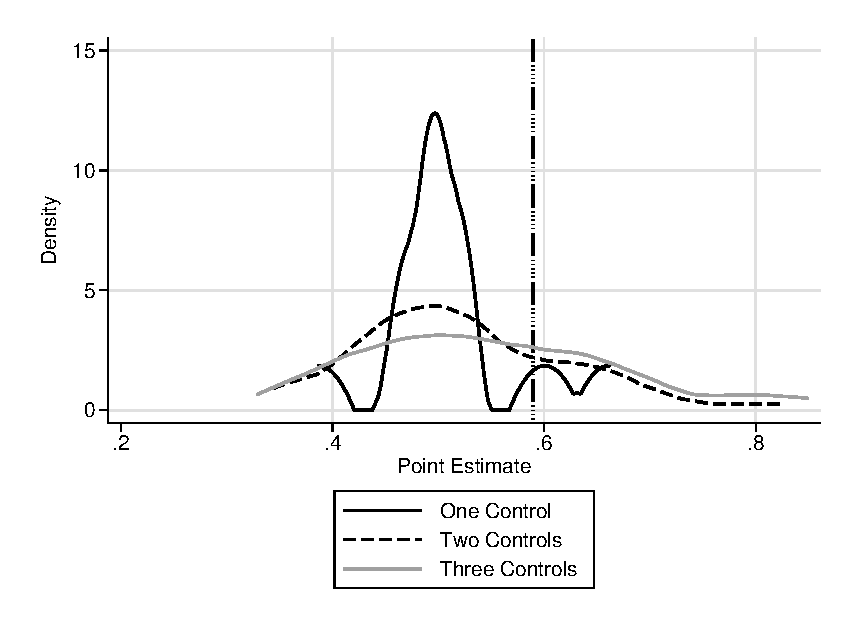
\includegraphics[width=\textwidth]{output/sencontrols_male_years_30y_itt_wctrl.eps}
\end{subfigure}%
\begin{subfigure}[h]{0.4\textwidth}
	\centering
	\caption{Employment, Males}
		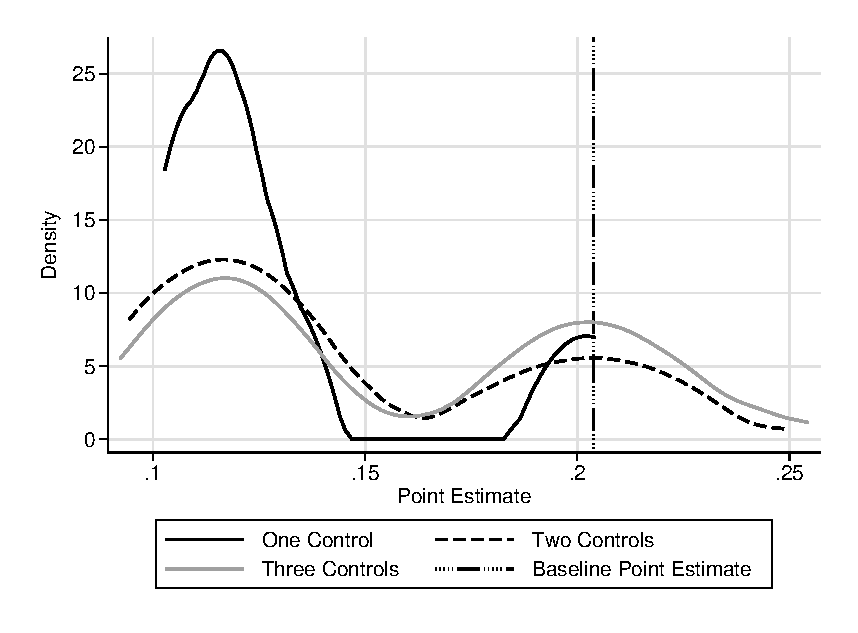
\includegraphics[width=\textwidth]{output/sencontrols_male_si30y_works_itt_wctrl.eps}
\end{subfigure}
\begin{subfigure}[h]{0.4\textwidth}
		\centering
		\caption{Years of Education, Females}
		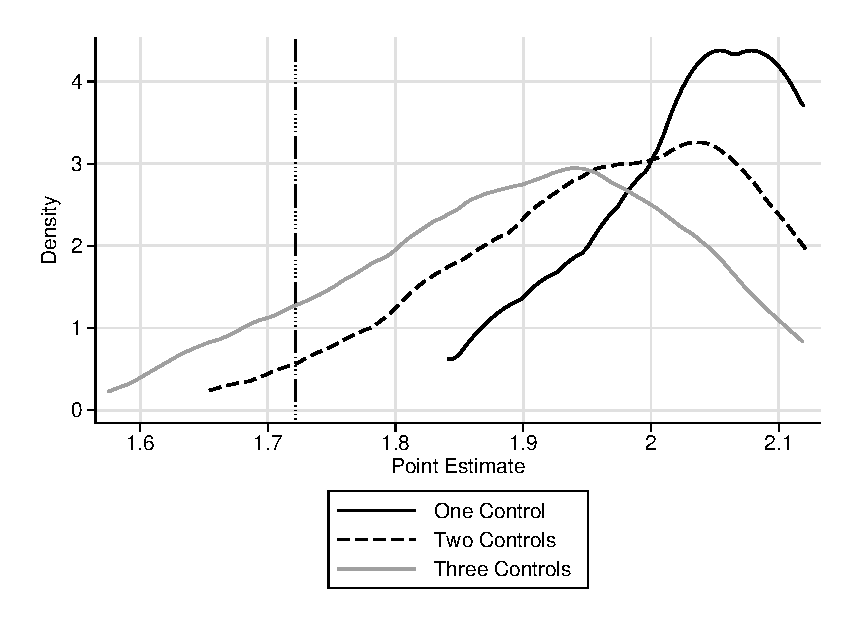
\includegraphics[width=\textwidth]{output/sencontrols_female_years_30y_itt_wctrl.eps}
\end{subfigure}%
\begin{subfigure}[h]{0.4\textwidth}
	\centering
	\caption{Employment, Females}
		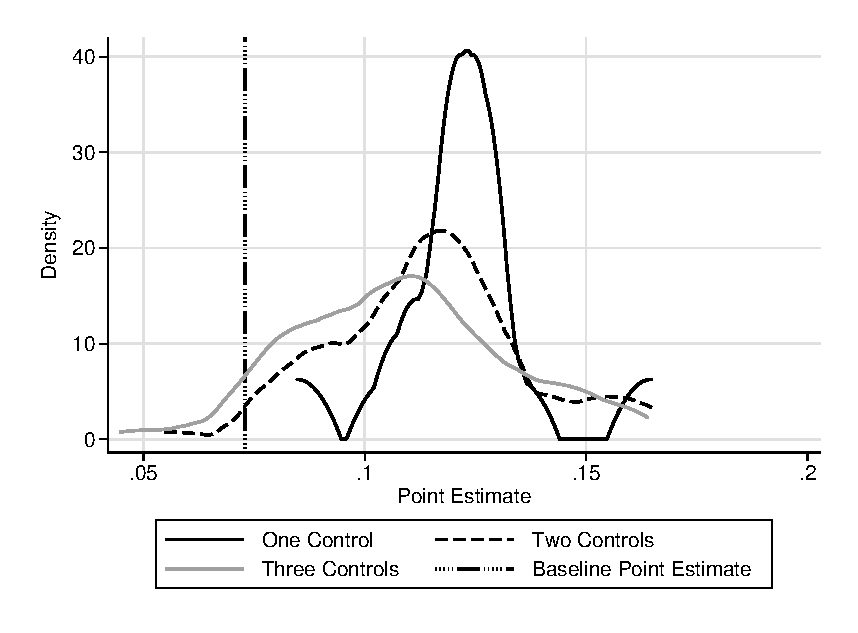
\includegraphics[width=\textwidth]{output/sencontrols_female_si30y_works_itt_wctrl.eps}
\end{subfigure}
\footnotesize \justify
Note: Panel (a) displays the distribution of the treatment effect estimate of the treatment compared to next best counterfactual for males years of education. The distribution is obtained by using all possible combinations of one, two, and three background variables listed in Table~\ref{tab:pselectvars}. In addition to these three variables, we account for a male indicator when computing estimates pooling males and females and a ABC/CARE indicator, to account for any difference in the programs---although we extensively document throughout the paper the similarities between them. The horizontal line marks the baseline estimate we use. The reminder panels present analogous distributions for the outcomes and genders indicated in the title.\\
\end{sidewaysfigure}

\begin{sidewaysfigure}[!htbp]
\centering
\caption{Sensitiviy to Choice of Control Set, Treatment vs. Stay at Home}
\begin{subfigure}[h]{0.4\textwidth}
		\centering
		\caption{Years of Education, Males}
		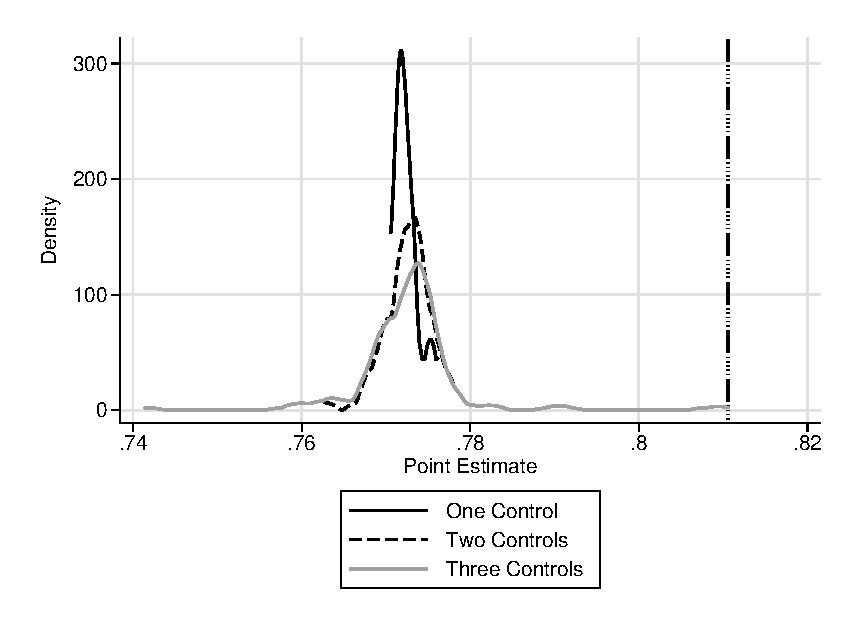
\includegraphics[width=\textwidth]{output/sencontrols_male_years_30y_epan_ipw_P0.eps}
\end{subfigure}%
\begin{subfigure}[h]{0.4\textwidth}
	\centering
	\caption{Employment, Males}
		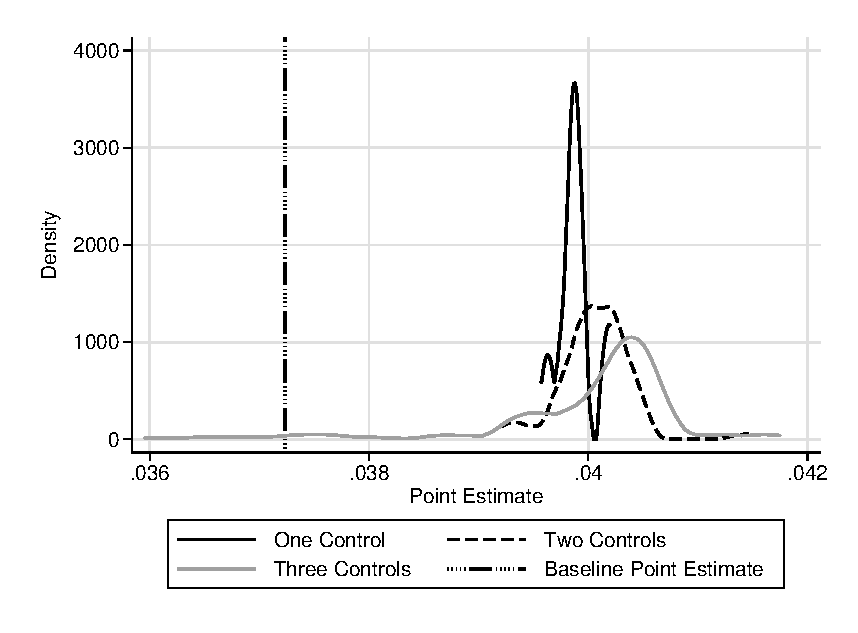
\includegraphics[width=\textwidth]{output/sencontrols_male_si30y_works_epan_ipw_P0.eps}
\end{subfigure}
\begin{subfigure}[h]{0.4\textwidth}
		\centering
		\caption{Years of Education, Females}
		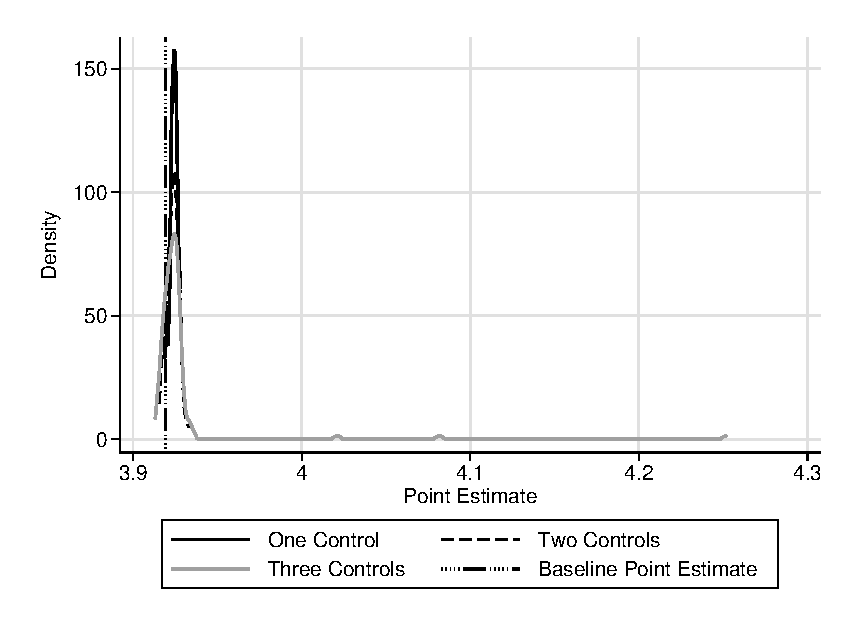
\includegraphics[width=\textwidth]{output/sencontrols_female_years_30y_epan_ipw_P0.eps}
\end{subfigure}%
\begin{subfigure}[h]{0.4\textwidth}
	\centering
	\caption{Employment, Females}
		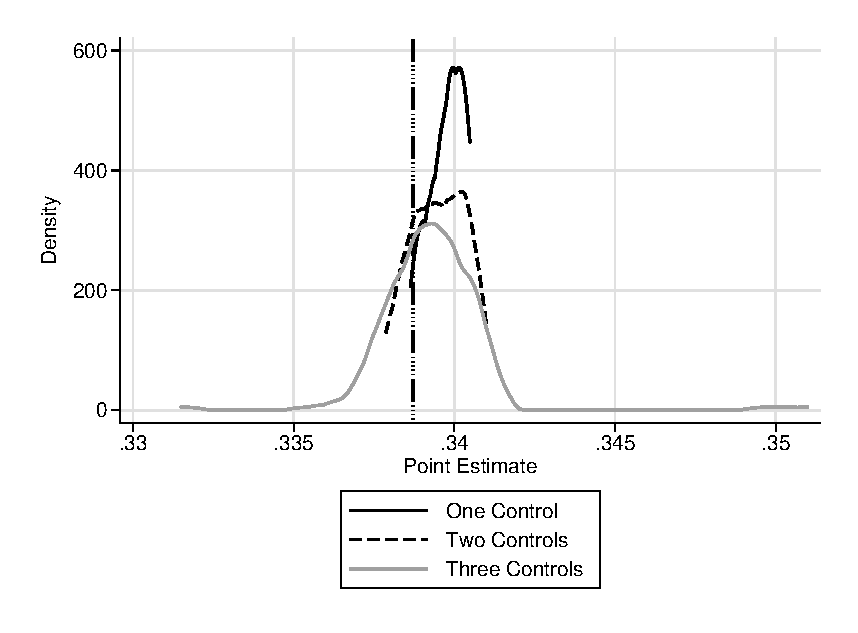
\includegraphics[width=\textwidth]{output/sencontrols_female_si30y_works_epan_ipw_P0.eps}
\end{subfigure}
\footnotesize \justify
Note: Panel (a) displays the distribution of the treatment effect estimate of the treatment compared to stay at home counterfactual for males years of education. The distribution is obtained by using all possible combinations of one, two, and three background variables listed in Table~\ref{tab:pselectvars}. In addition to these three variables, we account for a male indicator when computing estimates pooling males and females and a ABC/CARE indicator, to account for any difference in the programs---although we extensively document throughout the paper the similarities between them. We ``match'' and ``control'' using the same set of variables. The horizontal line marks the baseline estimate we use. The reminder panels present analogous distributions for the outcomes and genders indicated in the title.\\
\end{sidewaysfigure}

\begin{sidewaysfigure}[!htbp]
\centering
\caption{Sensitivity to Choice of Control Set, Treatment vs. Alternative Preschool}\label{fig:senstap}
\begin{subfigure}[h]{0.4\textwidth}
		\centering
		\caption{Years of Education, Males}
		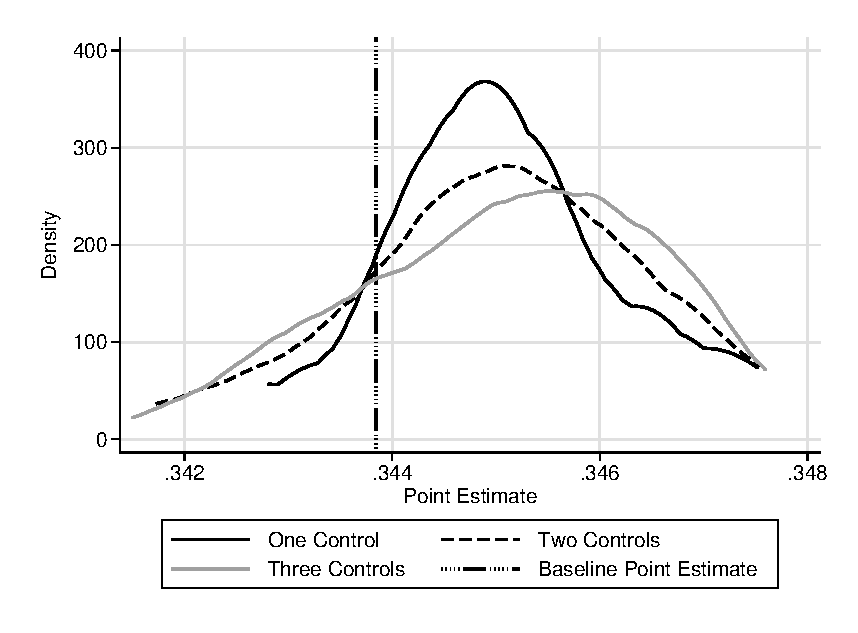
\includegraphics[width=\textwidth]{output/sencontrols_male_years_30y_epan_ipw_P1.eps}
\end{subfigure}%
\begin{subfigure}[h]{0.4\textwidth}
	\centering
	\caption{Employment, Males}
		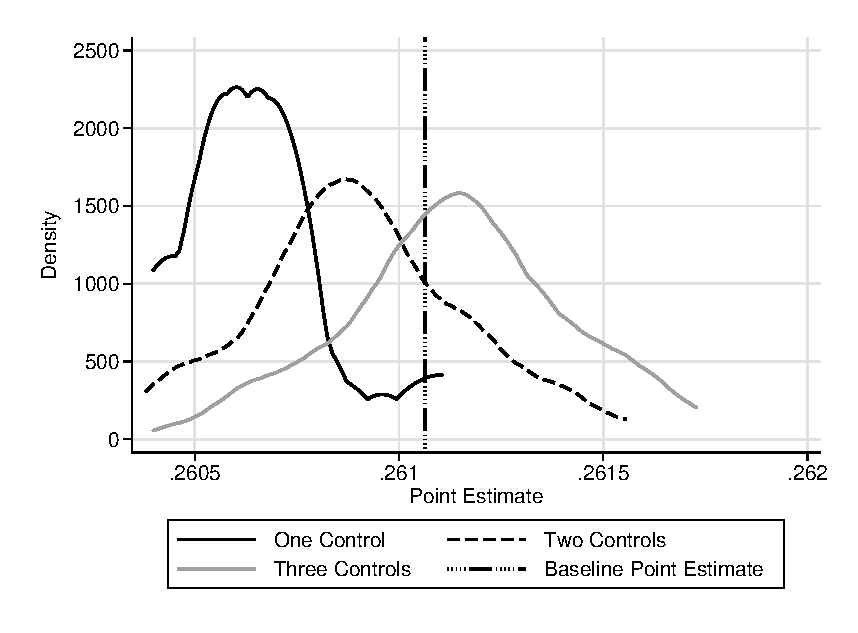
\includegraphics[width=\textwidth]{output/sencontrols_male_si30y_works_epan_ipw_P1.eps}
\end{subfigure}
\begin{subfigure}[h]{0.4\textwidth}
		\centering
		\caption{Years of Education, Females}
		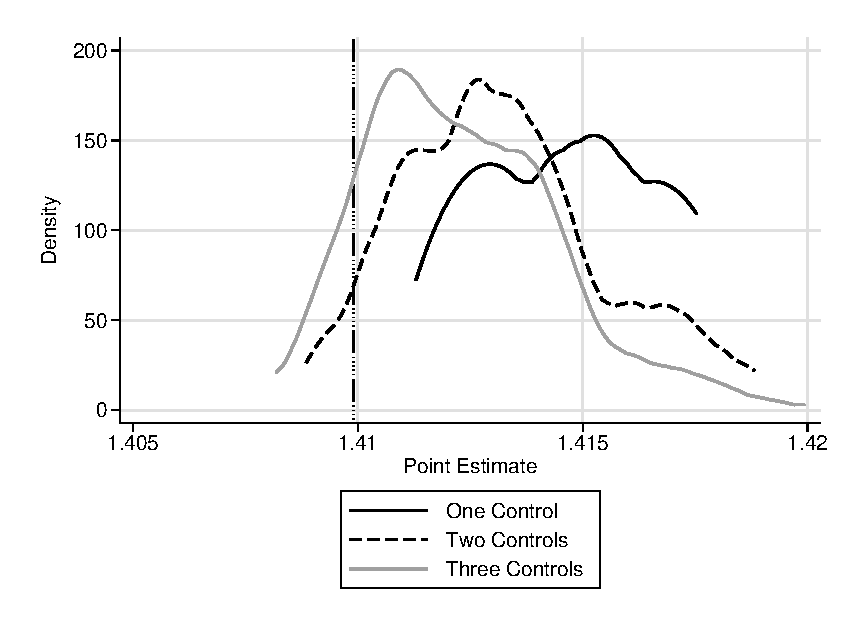
\includegraphics[width=\textwidth]{output/sencontrols_female_years_30y_epan_ipw_P1.eps}
\end{subfigure}%
\begin{subfigure}[h]{0.4\textwidth}
	\centering
	\caption{Employment, Females}
		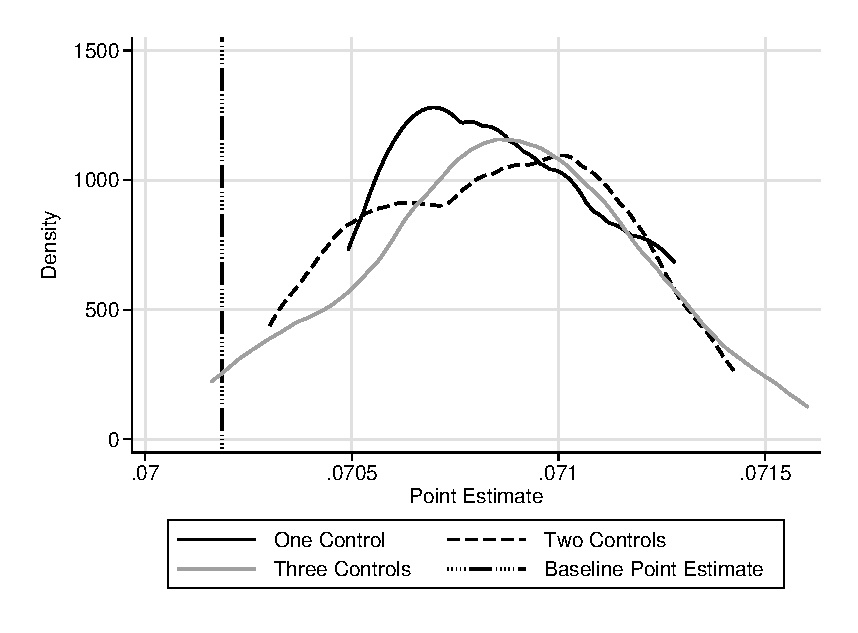
\includegraphics[width=\textwidth]{output/sencontrols_female_si30y_works_epan_ipw_P1.eps}
\end{subfigure}
\footnotesize \justify
Note: Panel (a) displays the distribution of the treatment effect estimate of the treatment compared to alternative preschool counterfactual for males years of education. The distribution is obtained by using all possible combinations of one, two, and three background variables listed in Table~\ref{tab:pselectvars}. In addition to these three variables, we account for a male indicator when computing estimates pooling males and females and a ABC/CARE indicator, to account for any difference in the programs---although we extensively document throughout the paper the similarities between them. We ``match'' and ``control'' using the same set of variables. The horizontal line marks the baseline estimate we use. The reminder panels present analogous distributions for the outcomes and genders indicated in the title.\\
\end{sidewaysfigure}

\subsection{Outcomes of Interest}

\noindent Table \ref{tab:main-outcomes} lists the 95 main outcomes that we test in our main analysis. We reverse the outcomes for which we consider a negative treatment effect socially positive. \\

\singlespacing
\begin{center}
\begin{ThreePartTable}

\begin{TableNotes}[para,flushleft]
Note: This table lists the outcomes that we test treatment effects for. We reverse the outcomes for which we consider a negative treatment effect socially positive.
\end{TableNotes}


\begin{longtable}{L{4cm} L{5cm} C{1cm} C{1cm} C{1.2cm} C{1.5cm}}

\caption{Outcome Variables} \\

\toprule
Category	&	Variable	&	Age	&	ABC	&	CARE	&	Reversed	\\ \midrule
\endfirsthead

\toprule
Category	&	Variable	&	Age	&	ABC	&	CARE	&	Reversed	\\ \midrule
\endhead

\midrule
\endfoot

%\bottomrule
\endlastfoot

IQ Scores	&	Std. IQ Test	&	2	&	\checkmark	&	\checkmark	&		\\
	&		&	2.5	&		&	\checkmark	&		\\
	&		&	3	&	\checkmark	&	\checkmark	&		\\
	&		&	3.5	&	\checkmark	&	\checkmark	&		\\
	&		&	4	&	\checkmark	&	\checkmark	&		\\
	&		&	4.5	&	\checkmark	&	\checkmark	&		\\
	&		&	5	&	\checkmark	&	\checkmark	&		\\
	&		&	6.6	&	\checkmark	&	\checkmark	&		\\
	&		&	7	&	\checkmark	&	\checkmark	&		\\
	&		&	8	&	\checkmark	&	\checkmark	&		\\
	&		&	12	&	\checkmark	&	\checkmark	&		\\
	&		&	15	&	\checkmark	&		&		\\
	&		&	21	&	\checkmark	&		&		\\
	&	IQ Factor	&	2 to 5	&	\checkmark	&	\checkmark	&		\\
	&		&	6 to 12	&	\checkmark	&	\checkmark	&		\\
	&		&	15 to 21	&	\checkmark	&		&		\\     
\\[0.1cm]
Achievement Scores	&	Std. Achv.  Test	&	5.5	&	\checkmark	&	\checkmark	&		\\
	&		&	6	&	\checkmark	&	\checkmark	&		\\
	&		&	6.5	&	\checkmark	&		&		\\
	&		&	7	&	\checkmark	&		&		\\
	&		&	7.5	&	\checkmark	&	\checkmark	&		\\
	&		&	8	&	\checkmark	&	\checkmark	&		\\
	&		&	8.5	&	\checkmark	&	\checkmark	&		\\
	&		&	12	&		&	\checkmark	&		\\
	&		&	15	&	\checkmark	&		&		\\
	&		&	21	&	\checkmark	&		&		\\
	&	PIAT Math Std. Score	&	7	&	\checkmark	&	\checkmark	&		\\
	&	Achievement Factor	&	5.5 to 12	&	\checkmark	&	\checkmark	&		\\
	&		&	15 to 21	&	\checkmark	&		&		\\
\\[0.1cm]
HOME Scores	&	HOME Score	&	0.5	&	\checkmark	&	\checkmark	&		\\
	&		&	1.5	&	\checkmark	&	\checkmark	&		\\
	&		&	2.5	&	\checkmark	&	\checkmark	&		\\
	&		&	3.5	&	\checkmark	&	\checkmark	&		\\
	&		&	4.5	&	\checkmark	&	\checkmark	&		\\
	&		&	8	&	\checkmark	&	\checkmark	&		\\
	&	HOME Factor	&	0.5 to 8	&	\checkmark	&	\checkmark	&		\\
\\[0.1cm]
Parent Income	&	Parental income	&	1.5	&	\checkmark	&	\checkmark	&		\\
	&		&	2.5	&	\checkmark	&	\checkmark	&		\\
	&		&	3.5	&	\checkmark	&	\checkmark	&		\\
	&		&	4.5	&	\checkmark	&	\checkmark	&		\\
	&		&	8	&	\checkmark	&		&		\\
	&		&	12	&	\checkmark	&		&		\\
	&		&	15	&	\checkmark	&		&		\\
	&	Parental Income Factor	&	1.5 to 15	&	\checkmark	&	\checkmark	&		\\
\\[0.1cm]
Mother's Employment	&	Mother Works	&	2	&	\checkmark	&	\checkmark	&		\\
	&		&	3	&	\checkmark	&	\checkmark	&		\\
	&		&	4	&	\checkmark	&	\checkmark	&		\\
	&		&	5	&	\checkmark	&	\checkmark	&		\\
	&		&	21	&	\checkmark	&		&		\\
	&	Mother Works Factor	&	2 to 21	&	\checkmark	&	\checkmark	&		\\
\\[0.1cm]
Mother's Education	&	Mother's Years of Edu.	&	2	&	\checkmark	&		&		\\
	&		&	3	&	\checkmark	&		&		\\
	&		&	4	&	\checkmark	&		&		\\
	&		&	5	&	\checkmark	&		&		\\
	&		&	9	&	\checkmark	&		&		\\
	&	Mother's Edu. Factor	&	2 to 9	&	\checkmark	&		&		\\
\\[0.1cm]
Father at Home	&	Father at Home	&	2	&	\checkmark	&	\checkmark	&		\\
	&		&	3	&	\checkmark	&	\checkmark	&		\\
	&		&	4	&	\checkmark	&	\checkmark	&		\\
	&		&	5	&	\checkmark	&	\checkmark	&		\\
	&		&	8	&	\checkmark	&	\checkmark	&		\\
	&	Father at Home Factor	&	2 to 8	&	\checkmark	&	\checkmark	&		\\
\\[0.1cm]
Adoption	&	Ever Adopted	&	       	&	\checkmark	&		&		\\
\\[0.1cm]
Education	&	Graduated High School	&	30	&	\checkmark	&	\checkmark	&		\\
	&	Attended Voc./Tech./Com. College	&	30	&	\checkmark	&	\checkmark	&		\\
	&	Graduated 4-year College	&	30	&	\checkmark	&	\checkmark	&		\\
	&	Years of Edu.	&	30	&	\checkmark	&	\checkmark	&		\\
	&	Education Factor	&	30	&	\checkmark	&	\checkmark	&		\\
\\[0.1cm]
Employment and Income	&	Employed	&	30	&	\checkmark	&	\checkmark	&		\\
	&	Labor Income	&	21	&	\checkmark	&	\checkmark	&		\\
	&		&	30	&	\checkmark	&	\checkmark	&		\\
	&	Public-Transfer Income	&	21	&	\checkmark	&	\checkmark	&	\checkmark	\\
	&		&	30	&	\checkmark	&	\checkmark	&	\checkmark	\\
	&	Employment Factor	&	21 to 30	&	\checkmark	&	\checkmark	&		\\
\\[0.1cm]
Crime	&	Total Felony Arrests	&	Mid-30s	&	\checkmark	&	\checkmark	&	\checkmark	\\
	&	Total Misdemeanor Arrests	&	Mid-30s	&	\checkmark	&	\checkmark	&	\checkmark	\\
	&	Total Years Incarcerated	&	30	&	\checkmark	&	\checkmark	&	\checkmark	\\
	&	Crime Factor	&	30 to Mid-30s	&	\checkmark	&	\checkmark	&	\checkmark	\\
\\[0.1cm]
Tobacco, Drugs, Alcohol	&	Cig. Smoked per day last month	&	30	&	\checkmark	&	\checkmark	&	\checkmark	\\
	&	Days drank alcohol last month	&	30	&	\checkmark	&	\checkmark	&	\checkmark	\\
	&	Days binge drank alcohol last month	&	30	&	\checkmark	&	\checkmark	&	\checkmark	\\
	&	Self-reported drug user	&	Mid-30s	&	\checkmark	&	\checkmark	&	\checkmark	\\
	&	Substance Use Factor	&	30 to Mid-30s	&	\checkmark	&	\checkmark	&	\checkmark	\\
\\[0.1cm]
Self-Reported Health	&	Self-reported Health	&	30	&	\checkmark	&	\checkmark	&	\checkmark	\\
	&		&	Mid-30s	&	\checkmark	&	\checkmark	&	\checkmark	\\
	&	Self-reported Health Factor	&	30 to Mid-30s	&	\checkmark	&	\checkmark	&	\checkmark	\\
\\[0.1cm]
Hypertension	&	Systolic Blood Pressure (mm Hg)	&	Mid-30s	&	\checkmark	&	\checkmark	&	\checkmark	\\
	&	Diastolic Blood Pressure (mm Hg)	&	Mid-30s	&	\checkmark	&	\checkmark	&	\checkmark	\\
	&	Prehypertension	&	Mid-30s	&	\checkmark	&	\checkmark	&	\checkmark	\\
	&	Hypertension	&	Mid-30s	&	\checkmark	&	\checkmark	&	\checkmark	\\
	&	Hypertension Factor	&	Mid-30s	&	\checkmark	&	\checkmark	&	\checkmark	\\
\\[0.1cm]
Cholesterol	&	High-Density Lipoprotein Chol. (mg/dL)	&	Mid-30s	&	\checkmark	&	\checkmark	&		\\
	&	Dyslipidemia	&	Mid-30s	&	\checkmark	&	\checkmark	&	\checkmark	\\
	&	Cholesterol Factor	&	Mid-30s	&	\checkmark	&	\checkmark	&	\checkmark	\\
\\[0.1cm]
Diabetes	&	Hemoglobin Level (\%)	&	Mid-30s	&	\checkmark	&	\checkmark	&	\checkmark	\\
	&	Prediabetes	&	Mid-30s	&	\checkmark	&	\checkmark	&	\checkmark	\\
	&	Diabetes	&	Mid-30s	&	\checkmark	&	\checkmark	&	\checkmark	\\
	&	Diabetes Factor	&	Mid-30s	&	\checkmark	&	\checkmark	&	\checkmark	\\
\\[0.1cm]
Vitamin D Deficiency	&	Vitamin D Deficiency	&	Mid-30s	&	\checkmark	&	\checkmark	&	\checkmark	\\
\\[0.1cm]
Obesity	&	Measured BMI	&	Mid-30s	&	\checkmark	&	\checkmark	&	\checkmark	\\
	&	Obesity	&	Mid-30s	&	\checkmark	&	\checkmark	&	\checkmark	\\
	&	Severe Obesity	&	Mid-30s	&	\checkmark	&	\checkmark	&	\checkmark	\\
	&	Waist-hip Ratio	&	Mid-30s	&	\checkmark	&	\checkmark	&	\checkmark	\\
	&	Abdominal Obesity	&	Mid-30s	&	\checkmark	&	\checkmark	&	\checkmark	\\
	&	Framingham Risk Score	&	Mid-30s	&	\checkmark	&	\checkmark	&	\checkmark	\\
	&	Obesity Factor	&	Mid-30s	&	\checkmark	&	\checkmark	&	\checkmark	\\
\\[0.1cm]
Mental Health (BSI)	&	Somatization	&	21	&	\checkmark	&	\checkmark	&	\checkmark	\\
	&		&	34	&	\checkmark	&	\checkmark	&	\checkmark	\\
	&	Depression	&	21	&	\checkmark	&	\checkmark	&	\checkmark	\\
	&		&	34	&	\checkmark	&	\checkmark	&	\checkmark	\\
	&	Anxiety	&	21	&	\checkmark	&	\checkmark	&	\checkmark	\\
	&		&	34	&	\checkmark	&	\checkmark	&	\checkmark	\\
	&	Hostility	&	21	&	\checkmark	&	\checkmark	&	\checkmark	\\
	&		&	34	&	\checkmark	&	\checkmark	&	\checkmark	\\
	&	Global Severity Index	&	21	&	\checkmark	&	\checkmark	&	\checkmark	\\
	&		&	34	&	\checkmark	&	\checkmark	&	\checkmark	\\
	&	Mental Health Factor	&	21 and 34	&	\checkmark	&	\checkmark	&	\checkmark	\\
\\[0.1cm]
Child Behavior (CAS)	&	Participates in Activity	&	12	&	\checkmark	&		&		\\
	&	Time Spent Reading	&	12	&	\checkmark	&		&		\\
	&	Good Description of Self	&	12	&	\checkmark	&		&		\\
	&	Views Self as Dumb	&	12	&	\checkmark	&		&	\checkmark	\\
	&	Views Self as Clumsy	&	12	&	\checkmark	&		&	\checkmark	\\
	&	Views Self as Not Liked	&	12	&	\checkmark	&		&	\checkmark	\\
	&	Proud About Self	&	12	&	\checkmark	&		&		\\
	&	Family Proud of You	&	12	&	\checkmark	&		&		\\
	&	Feels Inadequate, Inferior	&	12	&	\checkmark	&		&	\checkmark	\\
	&	Withdraws Excessively	&	12	&	\checkmark	&		&	\checkmark	\\
	&	Ignores Situation	&	12	&	\checkmark	&		&	\checkmark	\\
	&	Not Cope with Prob.	&	12	&	\checkmark	&		&	\checkmark	\\
	&	Often Mad of Angry	&	12	&	\checkmark	&		&	\checkmark	\\
	&	Impulsivity	&	12	&	\checkmark	&		&	\checkmark	\\
	&	Significant Fears	&	12	&	\checkmark	&		&	\checkmark	\\
	&	Denies Any Worries	&	12	&	\checkmark	&		&	\checkmark	\\

\bottomrule
	
\insertTableNotes
\end{longtable}
\end{ThreePartTable}
\end{center}




\doublespacing

\subsection{Estimates} \label{appendix:estimates}

\noindent Table~\ref{table:abccare_rslt_pooled_counts} shows that across all methods of estimation, pooling males and females, over 70\% of the treatment effect estimates are beneficial. When using a 10\% statistical significance level, almost 40\% of all estimates are beneficial. These statistics allow us to reject the hypothesis that there are no treatment effects. \\

\noindent For both males and females, we find positive effects in IQ test scores, achievement test scores, as well as educational attainment. Males also enjoy additional benefits in the areas of employment, labor earnings, and hypertension. \\

\noindent In each of the tables for combining functions and treatment effect estimates, we present 8 different estimates. Column (1) corresponds to the mean difference between the groups randomly assigned to receive center-based childcare and the groups randomly assigned not to. Column (2) adjusts the estimates in (1) for attrition and controls for a set of covariates. Column (3) corresponds to the mean difference between the groups randomly assigned to receive center-based childcare and the groups randomly assigned not to, restricting the latter to subjects who did not receive preschool alternatives. Column (4) adjusts the estimates in (3) for attrition and controls for a set of covariates. Column (5) corresponds to the mean difference between the groups randomly assigned to receive center-based childcare and the groups randomly assigned not to, placing a relatively high weight on the subjects who are likely not to be enrolled in alternative preschools. Column (6) corresponds to the mean difference between the groups randomly assigned to receive center-based childcare and the groups randomly assigned not to, restricting the latter to subjects who received preschool alternatives. Column (7) adjusts the estimates in (6) for attrition and controls for a set of covariates. Column (8) corresponds to the mean difference between the groups randomly assigned to receive center-based childcare and the groups randomly assigned not to, placing a relatively high weight on the children who are likely to be enrolled in alternative preschools. The results in bold are statistically significant at the 10\% level in a single-sided, non-parametric, bootstrapped test.\footnote{For the tables that present categorical combining function statistics that count the number of positive treatment effects that are significant at the 10\% level, two bootstrap tests are conducted. The first bootstrap test is used to determine significance at the 10\% level for each treatment effect. The second bootstrap test is used to determine whether the combined function statistic is significantly different from 10\% at the  10\% level. See Appendix~\ref{appendix:bootstrap} for more details on our inference procedures.} Columns (5) and (8) are standard kernel matching estimates. \\

\noindent Beginning with Table~\ref{table:abccare_rslt_pooled_cat0}, we display treatment effects by outcome. We divide the tables by different blocks of related outcomes. able~\ref{table:treatfactors} summarizes treatment effects on the set of selected``latent'' outcomes that we estimate. We display the full set of estimates beginning with Table~\ref{table:abccare_rslt_pooled_cat0}, together with the corresponding outcomes underlying the latents that we estimate.

%In each table we also present one or two factors constructed with the methodology in Appendix~\ref{app:endogeneity}. The idea behind doing this is to recover a ``latent'' outcome summarizing the outcomes in the table (e.g., latent IQ across IQ from ages 2 to 5). That is, measure the latent outcome using outcomes at various ages as measures of this latent. Testing for treatment effects on this factor it is yet another alternative to summarize treatment effects across a block of outcomes. T
\doublespacing


\subsection{Non-parametric Tests}\ref{app:subsection-nonparametric-tests}


\begin{table}[h!]
\centering
\begin{threeparttable}
\caption{Age Summary of Treatment-Control Comparisons by Gender, Full Set of Outcomes}\label{tab:rosenbaum-table-age-exp-TvC-big}
\begin{tabular}{l c c c c}
\toprule
 & Average & \% $ >0 $ & \% $ >0 $ , Significant & \citet{Rosenbaum_2005_Distribution_JRSS} \\
 & Effect Size & Treatment Effect & Treatment Effect & $ p $ -value \\
\midrule
\textbf{Childhood} & & & & \\
\quad Females &  \textbf{    0.233} & \textbf{   85.366} & \textbf{   41.463} & .602 \\
\quad Males &  \textbf{    0.222} & \textbf{   75.610} & \textbf{   34.146} & .469 \\
\midrule
\textbf{School Age} & & & & \\
\quad Females &  \textbf{    0.413} & \textbf{   88.889} & \textbf{   55.556} & .004 \\
\quad Males &  \textbf{    0.236} & \textbf{  100.000} & \textbf{   18.519} & .343 \\
\midrule
\textbf{Adulthood} & & & & \\
\quad Females &  \textbf{    0.222} & \textbf{   80.000} & \textbf{   42.500} & .004 \\
\quad Males &  \textbf{    0.124} & \textbf{   61.538} & \textbf{   20.513} & .343 \\
\midrule
\textbf{All} & & & & \\
\quad Females &  \textbf{    0.274} & \textbf{   84.259} & \textbf{   45.370} & .235 \\
\quad Males &  \textbf{    0.190} & \textbf{   76.636} & \textbf{   25.234} & .343 \\
\bottomrule
\end{tabular}
% This file generated by: /scripts/abccare/genderdifferences/abccare-gdiff-raw-rosenbaum-table-big.do

\begin{tablenotes}
\item Note:
\end{tablenotes}
\end{threeparttable}
\end{table}

\begin{table}[h!]
\centering
\begin{threeparttable}
\caption{Category Summary of Treatment-Control Comparisons by Gender, Full Set of Outcomes}\label{tab:rosenbaum-table-cats-exp-TvC-big}
\begin{tabular}{l c c c c}
\toprule
 & Average & \% $ >0 $ & \% $ >0 $ , Significant & \citet{Rosenbaum_2005_Distribution_JRSS} \\
 & Effect Size & Treatment Effect & Treatment Effect & $ p $ -value \\
\midrule
\textbf{IQ} & & & & \\
\quad Females &  \textbf{    0.674} & \textbf{  100.000} & \textbf{   75.000} & .046 \\
\quad Males &  \textbf{    0.421} & \textbf{  100.000} & \textbf{   58.333} & .235 \\
\midrule
\textbf{Achievement} & & & & \\
\quad Females &  \textbf{    0.804} & \textbf{  100.000} & \textbf{  100.000} & .01 \\
\quad Males &  \textbf{    0.217} & \textbf{  100.000} & \textbf{   40.000} & .812 \\
\midrule
\textbf{Social-emotional} & & & & \\
\quad Females &  \textbf{    0.176} & \textbf{   75.000} & \textbf{   37.500} & .01 \\
\quad Males &      0.053 & \textbf{   65.625} & \textbf{   12.500} & .812 \\
\midrule
\textbf{Parental Income} & & & & \\
\quad Females &  \textbf{    0.402} & \textbf{   92.308} & \textbf{   30.769} & .349 \\
\quad Males &  \textbf{    0.326} & \textbf{   92.308} & \textbf{   46.154} & .812 \\
\midrule
\textbf{Parenting} & & & & \\
\quad Females &  \textbf{    0.318} & \textbf{  100.000} & \textbf{   33.333} & .046 \\
\quad Males &  \textbf{    0.237} & \textbf{   83.333} &     0.000 & .812 \\
\midrule
\textbf{Education} & & & & \\
\quad Females &  \textbf{    0.261} & \textbf{   75.000} & \textbf{   25.000} & .046 \\
\quad Males &      0.075 & \textbf{   87.500} &     0.000 & .812 \\
\midrule
\textbf{Employment} & & & & \\
\quad Females &      0.170 & \textbf{  100.000} & \textbf{   33.333} & .046 \\
\quad Males &      0.206 & \textbf{   66.667} & \textbf{   33.333} & .812 \\
\midrule
\textbf{Crime} & & & & \\
\quad Females &  \textbf{    0.356} & \textbf{  100.000} & \textbf{  100.000} & .715 \\
\quad Males &      0.004 & \textbf{   33.333} &     0.000 & .812 \\
\midrule
\textbf{Risky Behavior} & & & & \\
\quad Females &      0.067 & \textbf{  100.000} &     0.000 & .469 \\
\quad Males &      0.232 & \textbf{   25.000} & \textbf{   25.000} & .086 \\
\midrule
\textbf{Health} & & & & \\
\quad Females &     -0.010 & \textbf{   64.706} & \textbf{   17.647} & .046 \\
\quad Males &     -0.249 & \textbf{   68.750} & \textbf{   25.000} & 0 \\
\bottomrule
\end{tabular}
% This file generated by: /scripts/abccare/genderdifferences/abccare-gdiff-raw-rosenbaum-table-big.do

\begin{tablenotes}
\item Note:
\end{tablenotes}
\end{threeparttable}
\end{table}

\begin{table}[h!]
\centering
\begin{threeparttable}
\caption{Age Summary of Treatment-Control (Stay at Home) Comparisons by Gender, Full Set of Outcomes}\label{tab:rosenbaum-table-age-exp-TvCh-big}
\begin{tabular}{l c c c c}
\toprule
 & Average & \% $ >0 $ & \% $ >0 $ , Significant & \citet{Rosenbaum_2005_Distribution_JRSS} \\
 & Effect Size & Treatment Effect & Treatment Effect & $ p $ -value \\
\midrule
\textbf{Childhood} & & & & \\
\quad Females &  \textbf{    0.192} & \textbf{   73.171} & \textbf{   51.220} & .061 \\
\quad Males &  \textbf{    0.320} & \textbf{   80.488} & \textbf{   46.341} & .394 \\
\midrule
\textbf{School Age} & & & & \\
\quad Females &  \textbf{    0.366} & \textbf{   96.296} & \textbf{   66.667} & .061 \\
\quad Males &  \textbf{    0.315} & \textbf{  100.000} & \textbf{   59.259} & .287 \\
\midrule
\textbf{Adulthood} & & & & \\
\quad Females &      0.093 & \textbf{   67.500} & \textbf{   40.000} & 0 \\
\quad Males &  \textbf{    0.206} & \textbf{   76.923} & \textbf{   38.462} & .053 \\
\midrule
\textbf{All} & & & & \\
\quad Females &  \textbf{    0.199} & \textbf{   76.852} & \textbf{   50.926} & .061 \\
\quad Males &  \textbf{    0.277} & \textbf{   84.112} & \textbf{   46.729} & .394 \\
\bottomrule
\end{tabular}
% This file generated by: /scripts/abccare/genderdifferences/abccare-gdiff-raw-rosenbaum-table-big.do

\begin{tablenotes}
\item Note:
\end{tablenotes}
\end{threeparttable}
\end{table}

\begin{table}[h!]
\centering
\begin{threeparttable}
\caption{Category Summary of Treatment-Control (Stay at Home) Comparisons by Gender, Full Set of Outcomes}\label{tab:rosenbaum-table-cats-exp-TvCh-big}
\begin{tabular}{l c c c c}
\toprule
 & Average & \% $ >0 $ & \% $ >0 $ , Significant & \citet{Rosenbaum_2005_Distribution_JRSS} \\
 & Effect Size & Treatment Effect & Treatment Effect & $ p $ -value \\
\midrule
\textbf{IQ} & & & & \\
\quad Females &  \textbf{    0.518} & \textbf{  100.000} & \textbf{   83.333} & .83 \\
\quad Males &  \textbf{    0.661} & \textbf{  100.000} & \textbf{   91.667} & .859 \\
\midrule
\textbf{Achievement} & & & & \\
\quad Females &  \textbf{    0.437} & \textbf{  100.000} & \textbf{  100.000} & .061 \\
\quad Males &  \textbf{    0.401} & \textbf{  100.000} & \textbf{   80.000} & .394 \\
\midrule
\textbf{Social-emotional} & & & & \\
\quad Females &      0.083 & \textbf{   65.625} & \textbf{   28.125} & .061 \\
\quad Males &  \textbf{    0.224} & \textbf{   78.125} & \textbf{   31.250} & .394 \\
\midrule
\textbf{Parental Income} & & & & \\
\quad Females &  \textbf{    0.291} & \textbf{   92.308} & \textbf{   76.923} & .305 \\
\quad Males &  \textbf{    0.280} & \textbf{   92.308} & \textbf{   61.538} & .394 \\
\midrule
\textbf{Parenting} & & & & \\
\quad Females &  \textbf{    0.242} & \textbf{  100.000} &    16.667 & .83 \\
\quad Males &  \textbf{    0.371} & \textbf{  100.000} & \textbf{   66.667} & .394 \\
\midrule
\textbf{Education} & & & & \\
\quad Females &  \textbf{    0.400} & \textbf{   75.000} & \textbf{   62.500} & .83 \\
\quad Males &  \textbf{    0.340} & \textbf{   87.500} &    12.500 & .394 \\
\midrule
\textbf{Employment} & & & & \\
\quad Females &      0.330 & \textbf{  100.000} &    33.333 & .83 \\
\quad Males &  \textbf{    0.257} & \textbf{   66.667} & \textbf{   33.333} & .394 \\
\midrule
\textbf{Crime} & & & & \\
\quad Females &     -0.144 & \textbf{   33.333} &     0.000 & .024 \\
\quad Males &  \textbf{    0.281} & \textbf{   66.667} & \textbf{   33.333} & .394 \\
\midrule
\textbf{Risky Behavior} & & & & \\
\quad Females &      0.049 & \textbf{   50.000} &    25.000 & .414 \\
\quad Males &      0.076 & \textbf{   50.000} & \textbf{   25.000} & .002 \\
\midrule
\textbf{Health} & & & & \\
\quad Females &  \textbf{    0.096} & \textbf{   58.824} & \textbf{   11.765} & .305 \\
\quad Males &      0.098 & \textbf{   75.000} & \textbf{   37.500} & 0 \\
\bottomrule
\end{tabular}
% This file generated by: /scripts/abccare/genderdifferences/abccare-gdiff-raw-rosenbaum-table-big.do

\begin{tablenotes}
\item Note:
\end{tablenotes}
\end{threeparttable}
\end{table}

\begin{table}[h!]
\centering
\begin{threeparttable}
\caption{Age Summary of Treatment-Control (Alternative Care) Comparisons by Gender, Full Set of Outcomes}\label{tab:rosenbaum-table-age-exp-TvCa-big}
\begin{tabular}{l c c c c}
\toprule
 & Average & \% $ >0 $ & \% $ >0 $ , Significant & \citet{Rosenbaum_2005_Distribution_JRSS} \\
 & Effect Size & Treatment Effect & Treatment Effect & $ p $ -value \\
\midrule
\textbf{Childhood} & & & & \\
\quad Females &  \textbf{    0.300} & \textbf{   85.366} & \textbf{   43.902} & .708 \\
\quad Males &      0.111 & \textbf{   63.415} & \textbf{   29.268} & .718 \\
\midrule
\textbf{School Age} & & & & \\
\quad Females &  \textbf{    0.466} & \textbf{   92.593} & \textbf{   70.370} & .025 \\
\quad Males &  \textbf{    0.285} & \textbf{   96.296} & \textbf{   44.444} & .448 \\
\midrule
\textbf{Adulthood} & & & & \\
\quad Females &  \textbf{    0.197} & \textbf{   77.500} & \textbf{   45.000} & .183 \\
\quad Males &      0.100 & \textbf{   62.500} & \textbf{   32.500} & .448 \\
\midrule
\textbf{All} & & & & \\
\quad Females &  \textbf{    0.304} & \textbf{   84.259} & \textbf{   50.926} & .429 \\
\quad Males &  \textbf{    0.150} & \textbf{   71.296} & \textbf{   34.259} & .448 \\
\bottomrule
\end{tabular}
% This file generated by: /scripts/abccare/genderdifferences/abccare-gdiff-raw-rosenbaum-table-big.do

\begin{tablenotes}
\item Note:
\end{tablenotes}
\end{threeparttable}
\end{table}

\begin{table}[h!]
\centering
\begin{threeparttable}
\caption{Category Summary of Treatment-Control (Alternative Care) Comparisons by Gender, Full Set of Outcomes}\label{tab:rosenbaum-table-cats-exp-TvCa-big}
\begin{tabular}{l c c c c}
\toprule
 & Average & \% $ >0 $ & \% $ >0 $ , Significant & \citet{Rosenbaum_2005_Distribution_JRSS} \\
 & Effect Size & Treatment Effect & Treatment Effect & $ p $ -value \\
\midrule
\textbf{IQ} & & & & \\
\quad Females &  \textbf{    0.737} & \textbf{  100.000} & \textbf{   91.667} & .183 \\
\quad Males &  \textbf{    0.440} & \textbf{  100.000} & \textbf{   83.333} & .448 \\
\midrule
\textbf{Achievement} & & & & \\
\quad Females &  \textbf{    0.638} & \textbf{  100.000} & \textbf{   80.000} & .311 \\
\quad Males &  \textbf{    0.345} & \textbf{  100.000} & \textbf{   40.000} & .718 \\
\midrule
\textbf{Social-emotional} & & & & \\
\quad Females &  \textbf{    0.220} & \textbf{   75.000} & \textbf{   46.875} & .025 \\
\quad Males &  \textbf{    0.146} & \textbf{   59.375} & \textbf{   15.625} & .718 \\
\midrule
\textbf{Parental Income} & & & & \\
\quad Females &  \textbf{    0.182} & \textbf{   92.308} & \textbf{   30.769} & .708 \\
\quad Males &  \textbf{    0.376} & \textbf{   92.308} & \textbf{   38.462} & .718 \\
\midrule
\textbf{Parenting} & & & & \\
\quad Females &      0.179 & \textbf{  100.000} &    16.667 & .052 \\
\quad Males &     -0.086 & \textbf{   66.667} & \textbf{   16.667} & .718 \\
\midrule
\textbf{Education} & & & & \\
\quad Females &  \textbf{    0.345} & \textbf{   87.500} & \textbf{   62.500} & .052 \\
\quad Males &      0.111 & \textbf{   75.000} & \textbf{   25.000} & .718 \\
\midrule
\textbf{Employment} & & & & \\
\quad Females &      0.033 & \textbf{   66.667} &     0.000 & .052 \\
\quad Males &  \textbf{    0.423} & \textbf{  100.000} & \textbf{   33.333} & .718 \\
\midrule
\textbf{Crime} & & & & \\
\quad Females &  \textbf{    0.450} & \textbf{  100.000} & \textbf{  100.000} & .898 \\
\quad Males &     -0.546 & \textbf{   33.333} &     0.000 & .448 \\
\midrule
\textbf{Risky Behavior} & & & & \\
\quad Females &  \textbf{    0.208} & \textbf{  100.000} &    25.000 & .708 \\
\quad Males &     -0.019 & \textbf{   25.000} & \textbf{   25.000} & .448 \\
\midrule
\textbf{Health} & & & & \\
\quad Females &      0.025 & \textbf{   64.706} & \textbf{   35.294} & .11 \\
\quad Males &  \textbf{    0.240} & \textbf{   52.941} & \textbf{   23.529} & .002 \\
\bottomrule
\end{tabular}
% This file generated by: /scripts/abccare/genderdifferences/abccare-gdiff-raw-rosenbaum-table-big.do

\begin{tablenotes}
\item Note:
\end{tablenotes}
\end{threeparttable}
\end{table}

\def\arraystretch{0.6}

\setlength\tabcolsep{0.3em}

\subsection{{Combining Functions - \% of Positive Treatment Effects, Aggregated}}
	\begin{table}[H]
     \caption{Combining Functions, Pooled Sample} 
     \label{table:abccare_rslt_pooled_counts}
	  \begin{tabular}{ccccccccc}
  \toprule

     & \scriptsize{(1)} & \scriptsize{(2)} & \scriptsize{(3)} & \scriptsize{(4)} & \scriptsize{(5)} & \scriptsize{(6)} & \scriptsize{(7)} & \scriptsize{(8)} \\ 
    \midrule  

    \mc{1}{l}{\scriptsize{\% Pos. TE}} & \mc{1}{c}{\scriptsize{77}} & \mc{1}{c}{\scriptsize{75}} & \mc{1}{c}{\scriptsize{77}} & \mc{1}{c}{\scriptsize{76}} & \mc{1}{c}{\scriptsize{74}} & \mc{1}{c}{\scriptsize{80}} & \mc{1}{c}{\scriptsize{72}} & \mc{1}{c}{\scriptsize{79}} \\  

     & \mc{1}{c}{\scriptsize{\textbf{(0.000)}}} & \mc{1}{c}{\scriptsize{\textbf{(0.000)}}} & \mc{1}{c}{\scriptsize{\textbf{(0.000)}}} & \mc{1}{c}{\scriptsize{\textbf{(0.000)}}} & \mc{1}{c}{\scriptsize{\textbf{(0.000)}}} & \mc{1}{c}{\scriptsize{\textbf{(0.000)}}} & \mc{1}{c}{\scriptsize{\textbf{(0.000)}}} & \mc{1}{c}{\scriptsize{\textbf{(0.000)}}} \\  

    \mc{1}{l}{\scriptsize{\% Pos. TE $|$ 10\% Significance}} & \mc{1}{c}{\scriptsize{53}} & \mc{1}{c}{\scriptsize{47}} & \mc{1}{c}{\scriptsize{38}} & \mc{1}{c}{\scriptsize{34}} & \mc{1}{c}{\scriptsize{39}} & \mc{1}{c}{\scriptsize{46}} & \mc{1}{c}{\scriptsize{41}} & \mc{1}{c}{\scriptsize{44}} \\  

     & \mc{1}{c}{\scriptsize{\textbf{(0.000)}}} & \mc{1}{c}{\scriptsize{\textbf{(0.000)}}} & \mc{1}{c}{\scriptsize{\textbf{(0.000)}}} & \mc{1}{c}{\scriptsize{\textbf{(0.000)}}} & \mc{1}{c}{\scriptsize{\textbf{(0.000)}}} & \mc{1}{c}{\scriptsize{\textbf{(0.000)}}} & \mc{1}{c}{\scriptsize{\textbf{(0.000)}}} & \mc{1}{c}{\scriptsize{\textbf{(0.000)}}} \\  

  \bottomrule
  \end{tabular}
	\end{table}  
\begin{spacing}{1}
\begin{footnotesize}
\noindent 	Note: This table presents estimates of the counts (combining functions) of (i) beneficial treatment effects and (ii) beneficial and significant (at the 10\% level) treatment effects. Counts for the different estimates described in Appendix~\ref{appendix:estimates} are presented in each column. For each count we present a $p$-value underneath. For the counts of beneficial treatment effects, the null hypothesis is that the count is 50\% (half of the treatment effects are positive). For the counts of significant at the 10\% level treatment effects, the null hypotheses is that 10\% of the treatment effects are positive and significant at the 10\% level. 
\end{footnotesize}
\end{spacing}

	\begin{table}[H]
     \caption{Combining Functions, Male Sample} 
     \label{table:abccare_rslt_male_counts}
	  \begin{tabular}{ccccccccc}
  \toprule

     & \scriptsize{(1)} & \scriptsize{(2)} & \scriptsize{(3)} & \scriptsize{(4)} & \scriptsize{(5)} & \scriptsize{(6)} & \scriptsize{(7)} & \scriptsize{(8)} \\ 
    \midrule  

    \mc{1}{l}{\scriptsize{\% Pos. TE}} & \mc{1}{c}{\scriptsize{72}} & \mc{1}{c}{\scriptsize{70}} & \mc{1}{c}{\scriptsize{53}} & \mc{1}{c}{\scriptsize{54}} & \mc{1}{c}{\scriptsize{49}} & \mc{1}{c}{\scriptsize{75}} & \mc{1}{c}{\scriptsize{73}} & \mc{1}{c}{\scriptsize{74}} \\  

     & \mc{1}{c}{\scriptsize{\textbf{(0.000)}}} & \mc{1}{c}{\scriptsize{\textbf{(0.000)}}} & \mc{1}{c}{\scriptsize{(0.359)}} & \mc{1}{c}{\scriptsize{(0.345)}} & \mc{1}{c}{\scriptsize{(0.571)}} & \mc{1}{c}{\scriptsize{\textbf{(0.000)}}} & \mc{1}{c}{\scriptsize{\textbf{(0.000)}}} & \mc{1}{c}{\scriptsize{\textbf{(0.000)}}} \\  

    \mc{1}{l}{\scriptsize{\% Pos. TE $|$ 10\% Significance}} & \mc{1}{c}{\scriptsize{30}} & \mc{1}{c}{\scriptsize{30}} & \mc{1}{c}{\scriptsize{18}} & \mc{1}{c}{\scriptsize{17}} & \mc{1}{c}{\scriptsize{17}} & \mc{1}{c}{\scriptsize{31}} & \mc{1}{c}{\scriptsize{30}} & \mc{1}{c}{\scriptsize{28}} \\  

     & \mc{1}{c}{\scriptsize{\textbf{(0.001)}}} & \mc{1}{c}{\scriptsize{\textbf{(0.000)}}} & \mc{1}{c}{\scriptsize{(0.110)}} & \mc{1}{c}{\scriptsize{(0.160)}} & \mc{1}{c}{\scriptsize{(0.118)}} & \mc{1}{c}{\scriptsize{\textbf{(0.003)}}} & \mc{1}{c}{\scriptsize{\textbf{(0.000)}}} & \mc{1}{c}{\scriptsize{\textbf{(0.011)}}} \\  

  \bottomrule
  \end{tabular}
	\end{table}
\singlespacing
\begin{spacing}{1}
\begin{footnotesize}
\noindent 	Note: This table presents estimates of the counts (combining functions) of (i) beneficial treatment effects and (ii) beneficial and significant (at the 10\% level) treatment effects. Counts for the different estimates described in Appendix~\ref{appendix:estimates} are presented in each column. For each count we present a $p$-value underneath. For the counts of beneficial treatment effects, the null hypothesis is that the count is 50\% (half of the treatment effects are positive). For the counts of significant at the 10\% level treatment effects, the null hypotheses is that 10\% of the treatment effects are positive and significant at the 10\% level. 
\end{footnotesize}
\end{spacing}

	\begin{table}[H]
     \caption{Combining Functions, Female Sample} 
     \label{table:abccare_rslt_female_counts}
	  \begin{tabular}{ccccccccc}
  \toprule

     & \scriptsize{(1)} & \scriptsize{(2)} & \scriptsize{(3)} & \scriptsize{(4)} & \scriptsize{(5)} & \scriptsize{(6)} & \scriptsize{(7)} & \scriptsize{(8)} \\ 
    \midrule  

    \mc{1}{l}{\scriptsize{\% Pos. TE}} & \mc{1}{c}{\scriptsize{83}} & \mc{1}{c}{\scriptsize{73}} & \mc{1}{c}{\scriptsize{78}} & \mc{1}{c}{\scriptsize{78}} & \mc{1}{c}{\scriptsize{79}} & \mc{1}{c}{\scriptsize{82}} & \mc{1}{c}{\scriptsize{69}} & \mc{1}{c}{\scriptsize{79}} \\  

     & \mc{1}{c}{\scriptsize{\textbf{(0.000)}}} & \mc{1}{c}{\scriptsize{\textbf{(0.000)}}} & \mc{1}{c}{\scriptsize{\textbf{(0.000)}}} & \mc{1}{c}{\scriptsize{\textbf{(0.000)}}} & \mc{1}{c}{\scriptsize{\textbf{(0.000)}}} & \mc{1}{c}{\scriptsize{\textbf{(0.000)}}} & \mc{1}{c}{\scriptsize{\textbf{(0.003)}}} & \mc{1}{c}{\scriptsize{\textbf{(0.000)}}} \\  

    \mc{1}{l}{\scriptsize{\% Pos. TE $|$ 10\% Significance}} & \mc{1}{c}{\scriptsize{50}} & \mc{1}{c}{\scriptsize{31}} & \mc{1}{c}{\scriptsize{50}} & \mc{1}{c}{\scriptsize{48}} & \mc{1}{c}{\scriptsize{53}} & \mc{1}{c}{\scriptsize{39}} & \mc{1}{c}{\scriptsize{19}} & \mc{1}{c}{\scriptsize{29}} \\  

     & \mc{1}{c}{\scriptsize{\textbf{(0.000)}}} & \mc{1}{c}{\scriptsize{\textbf{(0.000)}}} & \mc{1}{c}{\scriptsize{\textbf{(0.000)}}} & \mc{1}{c}{\scriptsize{\textbf{(0.000)}}} & \mc{1}{c}{\scriptsize{\textbf{(0.000)}}} & \mc{1}{c}{\scriptsize{\textbf{(0.000)}}} & \mc{1}{c}{\scriptsize{\textbf{(0.066)}}} & \mc{1}{c}{\scriptsize{\textbf{(0.004)}}} \\  

  \bottomrule
  \end{tabular}
	\end{table}  
\begin{spacing}{1}
\begin{footnotesize}
\noindent 	Note: This table presents estimates of the counts (combining functions) of (i) beneficial treatment effects and (ii) beneficial and significant (at the 10\% level) treatment effects. Counts for the different estimates described in Appendix~\ref{appendix:estimates} are presented in each column. For each count we present a $p$-value underneath. For the counts of beneficial treatment effects, the null hypothesis is that the count is 50\% (half of the treatment effects are positive). For the counts of significant at the 10\% level treatment effects, the null hypotheses is that 10\% of the treatment effects are positive and significant at the 10\% level. 
\end{footnotesize}
\end{spacing}
\clearpage

\subsection{{Combining Functions - \% of Positive Treatment Effects, by Category}}


	\begin{table}[H]
     \caption{Combining Functions by Category, Pooled Sample} 
     \label{table:abccare_rslt_pooled_counts_n50a100}
	  \begin{tabular}{cccccccccc}
  \toprule

    \scriptsize{Category} & \scriptsize{(1)} & \scriptsize{(2)} & \scriptsize{(3)} & \scriptsize{(4)} & \scriptsize{(5)} & \scriptsize{(6)} & \scriptsize{(7)} & \scriptsize{(8)} & \scriptsize{N} \\ 
    \midrule  

    \mc{1}{l}{\scriptsize{Cognitive Skills}} & \mc{1}{c}{\scriptsize{92}} & \mc{1}{c}{\scriptsize{92}} & \mc{1}{c}{\scriptsize{92}} & \mc{1}{c}{\scriptsize{92}} & \mc{1}{c}{\scriptsize{92}} & \mc{1}{c}{\scriptsize{92}} & \mc{1}{c}{\scriptsize{92}} & \mc{1}{c}{\scriptsize{92}} & \mc{1}{c}{\scriptsize{26}} \\  

     & \mc{1}{c}{\scriptsize{\textbf{(0.000)}}} & \mc{1}{c}{\scriptsize{\textbf{(0.000)}}} & \mc{1}{c}{\scriptsize{\textbf{(0.000)}}} & \mc{1}{c}{\scriptsize{\textbf{(0.000)}}} & \mc{1}{c}{\scriptsize{\textbf{(0.000)}}} & \mc{1}{c}{\scriptsize{\textbf{(0.000)}}} & \mc{1}{c}{\scriptsize{\textbf{(0.000)}}} & \mc{1}{c}{\scriptsize{\textbf{(0.000)}}} &  \\  

    \mc{1}{l}{\scriptsize{Childhood Household Environment}} & \mc{1}{c}{\scriptsize{62}} & \mc{1}{c}{\scriptsize{62}} & \mc{1}{c}{\scriptsize{54}} & \mc{1}{c}{\scriptsize{54}} & \mc{1}{c}{\scriptsize{54}} & \mc{1}{c}{\scriptsize{85}} & \mc{1}{c}{\scriptsize{46}} & \mc{1}{c}{\scriptsize{92}} & \mc{1}{c}{\scriptsize{13}} \\  

     & \mc{1}{c}{\scriptsize{(0.194)}} & \mc{1}{c}{\scriptsize{(0.237)}} & \mc{1}{c}{\scriptsize{(0.194)}} & \mc{1}{c}{\scriptsize{(0.113)}} & \mc{1}{c}{\scriptsize{(0.155)}} & \mc{1}{c}{\scriptsize{\textbf{(0.076)}}} & \mc{1}{c}{\scriptsize{(0.604)}} & \mc{1}{c}{\scriptsize{\textbf{(0.000)}}} &  \\  

    \mc{1}{l}{\scriptsize{Mother's Employment, Education, and Income}} & \mc{1}{c}{\scriptsize{87}} & \mc{1}{c}{\scriptsize{87}} & \mc{1}{c}{\scriptsize{87}} & \mc{1}{c}{\scriptsize{87}} & \mc{1}{c}{\scriptsize{93}} & \mc{1}{c}{\scriptsize{87}} & \mc{1}{c}{\scriptsize{73}} & \mc{1}{c}{\scriptsize{87}} & \mc{1}{c}{\scriptsize{15}} \\  

     & \mc{1}{c}{\scriptsize{\textbf{(0.000)}}} & \mc{1}{c}{\scriptsize{\textbf{(0.000)}}} & \mc{1}{c}{\scriptsize{\textbf{(0.000)}}} & \mc{1}{c}{\scriptsize{\textbf{(0.000)}}} & \mc{1}{c}{\scriptsize{\textbf{(0.000)}}} & \mc{1}{c}{\scriptsize{\textbf{(0.000)}}} & \mc{1}{c}{\scriptsize{\textbf{(0.085)}}} & \mc{1}{c}{\scriptsize{\textbf{(0.000)}}} &  \\  

    \mc{1}{l}{\scriptsize{Education, Employment, Income}} & \mc{1}{c}{\scriptsize{87}} & \mc{1}{c}{\scriptsize{80}} & \mc{1}{c}{\scriptsize{87}} & \mc{1}{c}{\scriptsize{80}} & \mc{1}{c}{\scriptsize{80}} & \mc{1}{c}{\scriptsize{87}} & \mc{1}{c}{\scriptsize{87}} & \mc{1}{c}{\scriptsize{87}} & \mc{1}{c}{\scriptsize{15}} \\  

     & \mc{1}{c}{\scriptsize{\textbf{(0.000)}}} & \mc{1}{c}{\scriptsize{\textbf{(0.000)}}} & \mc{1}{c}{\scriptsize{\textbf{(0.000)}}} & \mc{1}{c}{\scriptsize{\textbf{(0.000)}}} & \mc{1}{c}{\scriptsize{\textbf{(0.000)}}} & \mc{1}{c}{\scriptsize{\textbf{(0.000)}}} & \mc{1}{c}{\scriptsize{\textbf{(0.000)}}} & \mc{1}{c}{\scriptsize{\textbf{(0.000)}}} &  \\  

    \mc{1}{l}{\scriptsize{Crime}} & \mc{1}{c}{\scriptsize{25}} & \mc{1}{c}{\scriptsize{25}} & \mc{1}{c}{\scriptsize{75}} & \mc{1}{c}{\scriptsize{50}} & \mc{1}{c}{\scriptsize{25}} & \mc{1}{c}{\scriptsize{25}} & \mc{1}{c}{\scriptsize{25}} & \mc{1}{c}{\scriptsize{25}} & \mc{1}{c}{\scriptsize{4}} \\  

     & \mc{1}{c}{\scriptsize{(0.971)}} & \mc{1}{c}{\scriptsize{(0.893)}} & \mc{1}{c}{\scriptsize{\textbf{(0.000)}}} & \mc{1}{c}{\scriptsize{(0.521)}} & \mc{1}{c}{\scriptsize{(0.890)}} & \mc{1}{c}{\scriptsize{(0.940)}} & \mc{1}{c}{\scriptsize{(0.811)}} & \mc{1}{c}{\scriptsize{(0.886)}} &  \\  

    \mc{1}{l}{\scriptsize{Drugs and Alcohol}} & \mc{1}{c}{\scriptsize{20}} & \mc{1}{c}{\scriptsize{40}} & \mc{1}{c}{\scriptsize{80}} & \mc{1}{c}{\scriptsize{80}} & \mc{1}{c}{\scriptsize{60}} & \mc{1}{c}{\scriptsize{20}} & \mc{1}{c}{\scriptsize{20}} & \mc{1}{c}{\scriptsize{20}} & \mc{1}{c}{\scriptsize{5}} \\  

     & \mc{1}{c}{\scriptsize{(0.986)}} & \mc{1}{c}{\scriptsize{(0.661)}} & \mc{1}{c}{\scriptsize{\textbf{(0.090)}}} & \mc{1}{c}{\scriptsize{\textbf{(0.073)}}} & \mc{1}{c}{\scriptsize{(0.307)}} & \mc{1}{c}{\scriptsize{(0.938)}} & \mc{1}{c}{\scriptsize{(0.909)}} & \mc{1}{c}{\scriptsize{(0.942)}} &  \\  

    \mc{1}{l}{\scriptsize{Adult Health}} & \mc{1}{c}{\scriptsize{63}} & \mc{1}{c}{\scriptsize{63}} & \mc{1}{c}{\scriptsize{47}} & \mc{1}{c}{\scriptsize{47}} & \mc{1}{c}{\scriptsize{47}} & \mc{1}{c}{\scriptsize{63}} & \mc{1}{c}{\scriptsize{53}} & \mc{1}{c}{\scriptsize{53}} & \mc{1}{c}{\scriptsize{19}} \\  

     & \mc{1}{c}{\scriptsize{(0.193)}} & \mc{1}{c}{\scriptsize{(0.175)}} & \mc{1}{c}{\scriptsize{(0.611)}} & \mc{1}{c}{\scriptsize{(0.636)}} & \mc{1}{c}{\scriptsize{(0.585)}} & \mc{1}{c}{\scriptsize{(0.197)}} & \mc{1}{c}{\scriptsize{(0.412)}} & \mc{1}{c}{\scriptsize{(0.488)}} &  \\  

    \mc{1}{l}{\scriptsize{Mental Health}} & \mc{1}{c}{\scriptsize{100}} & \mc{1}{c}{\scriptsize{100}} & \mc{1}{c}{\scriptsize{91}} & \mc{1}{c}{\scriptsize{90}} & \mc{1}{c}{\scriptsize{91}} & \mc{1}{c}{\scriptsize{100}} & \mc{1}{c}{\scriptsize{100}} & \mc{1}{c}{\scriptsize{100}} & \mc{1}{c}{\scriptsize{11}} \\  

     & \mc{1}{c}{\scriptsize{\textbf{(0.000)}}} & \mc{1}{c}{\scriptsize{\textbf{(0.000)}}} & \mc{1}{c}{\scriptsize{\textbf{(0.000)}}} & \mc{1}{c}{\scriptsize{\textbf{(0.000)}}} & \mc{1}{c}{\scriptsize{\textbf{(0.000)}}} & \mc{1}{c}{\scriptsize{\textbf{(0.000)}}} & \mc{1}{c}{\scriptsize{\textbf{(0.000)}}} & \mc{1}{c}{\scriptsize{\textbf{(0.000)}}} &  \\  

  \bottomrule
  \end{tabular}
	\end{table}
\begin{spacing}{1}
\begin{footnotesize}
\noindent Note: This table presents estimates of the counts (combining functions) of beneficial treatment effects by the categories of outcomes in each row. The last column presents the number of outcomes per category. Counts for the different estimates described in Appendix~\ref{appendix:estimates} are presented in each column. For each count we present a $p$-value underneath. The null hypothesis is that the count is 50\% (half of the treatment effects are positive).
\end{footnotesize}
\end{spacing}   

	\begin{table}[H]
     \caption{Combining Functions by Category $|$ 10\% Significance, Pooled Sample} 
     \label{table:abccare_rslt_pooled_counts_n10a10}
	  \begin{tabular}{cccccccccc}
  \toprule

    \scriptsize{Category} & \scriptsize{(1)} & \scriptsize{(2)} & \scriptsize{(3)} & \scriptsize{(4)} & \scriptsize{(5)} & \scriptsize{(6)} & \scriptsize{(7)} & \scriptsize{(8)} & \scriptsize{N} \\ 
    \midrule  

    \mc{1}{l}{\scriptsize{Cognitive Skills}} & \mc{1}{c}{\scriptsize{88}} & \mc{1}{c}{\scriptsize{85}} & \mc{1}{c}{\scriptsize{58}} & \mc{1}{c}{\scriptsize{69}} & \mc{1}{c}{\scriptsize{65}} & \mc{1}{c}{\scriptsize{88}} & \mc{1}{c}{\scriptsize{81}} & \mc{1}{c}{\scriptsize{88}} & \mc{1}{c}{\scriptsize{26}} \\  

     & \mc{1}{c}{\scriptsize{\textbf{(0.000)}}} & \mc{1}{c}{\scriptsize{\textbf{(0.000)}}} & \mc{1}{c}{\scriptsize{\textbf{(0.000)}}} & \mc{1}{c}{\scriptsize{\textbf{(0.000)}}} & \mc{1}{c}{\scriptsize{\textbf{(0.000)}}} & \mc{1}{c}{\scriptsize{\textbf{(0.000)}}} & \mc{1}{c}{\scriptsize{\textbf{(0.000)}}} & \mc{1}{c}{\scriptsize{\textbf{(0.000)}}} &  \\  

    \mc{1}{l}{\scriptsize{Childhood Household Environment}} & \mc{1}{c}{\scriptsize{23}} & \mc{1}{c}{\scriptsize{0}} & \mc{1}{c}{\scriptsize{38}} & \mc{1}{c}{\scriptsize{38}} & \mc{1}{c}{\scriptsize{46}} & \mc{1}{c}{\scriptsize{8}} & \mc{1}{c}{\scriptsize{0}} & \mc{1}{c}{\scriptsize{15}} & \mc{1}{c}{\scriptsize{13}} \\  

     & \mc{1}{c}{\scriptsize{(0.235)}} & \mc{1}{c}{\scriptsize{(1.000)}} & \mc{1}{c}{\scriptsize{\textbf{(0.000)}}} & \mc{1}{c}{\scriptsize{\textbf{(0.000)}}} & \mc{1}{c}{\scriptsize{\textbf{(0.000)}}} & \mc{1}{c}{\scriptsize{(0.318)}} & \mc{1}{c}{\scriptsize{(1.000)}} & \mc{1}{c}{\scriptsize{(0.303)}} &  \\  

    \mc{1}{l}{\scriptsize{Mother's Employment, Education, and Income}} & \mc{1}{c}{\scriptsize{53}} & \mc{1}{c}{\scriptsize{40}} & \mc{1}{c}{\scriptsize{53}} & \mc{1}{c}{\scriptsize{53}} & \mc{1}{c}{\scriptsize{53}} & \mc{1}{c}{\scriptsize{27}} & \mc{1}{c}{\scriptsize{20}} & \mc{1}{c}{\scriptsize{40}} & \mc{1}{c}{\scriptsize{15}} \\  

     & \mc{1}{c}{\scriptsize{\textbf{(0.005)}}} & \mc{1}{c}{\scriptsize{\textbf{(0.021)}}} & \mc{1}{c}{\scriptsize{\textbf{(0.001)}}} & \mc{1}{c}{\scriptsize{\textbf{(0.002)}}} & \mc{1}{c}{\scriptsize{\textbf{(0.003)}}} & \mc{1}{c}{\scriptsize{(0.145)}} & \mc{1}{c}{\scriptsize{(0.175)}} & \mc{1}{c}{\scriptsize{\textbf{(0.057)}}} &  \\  

    \mc{1}{l}{\scriptsize{Education, Employment, Income}} & \mc{1}{c}{\scriptsize{67}} & \mc{1}{c}{\scriptsize{47}} & \mc{1}{c}{\scriptsize{40}} & \mc{1}{c}{\scriptsize{47}} & \mc{1}{c}{\scriptsize{53}} & \mc{1}{c}{\scriptsize{60}} & \mc{1}{c}{\scriptsize{40}} & \mc{1}{c}{\scriptsize{60}} & \mc{1}{c}{\scriptsize{15}} \\  

     & \mc{1}{c}{\scriptsize{\textbf{(0.000)}}} & \mc{1}{c}{\scriptsize{\textbf{(0.002)}}} & \mc{1}{c}{\scriptsize{\textbf{(0.018)}}} & \mc{1}{c}{\scriptsize{\textbf{(0.002)}}} & \mc{1}{c}{\scriptsize{\textbf{(0.001)}}} & \mc{1}{c}{\scriptsize{\textbf{(0.000)}}} & \mc{1}{c}{\scriptsize{\textbf{(0.045)}}} & \mc{1}{c}{\scriptsize{\textbf{(0.000)}}} &  \\  

    \mc{1}{l}{\scriptsize{Crime}} & \mc{1}{c}{\scriptsize{25}} & \mc{1}{c}{\scriptsize{0}} & \mc{1}{c}{\scriptsize{0}} & \mc{1}{c}{\scriptsize{0}} & \mc{1}{c}{\scriptsize{0}} & \mc{1}{c}{\scriptsize{25}} & \mc{1}{c}{\scriptsize{0}} & \mc{1}{c}{\scriptsize{0}} & \mc{1}{c}{\scriptsize{4}} \\  

     & \mc{1}{c}{\scriptsize{\textbf{(0.000)}}} & \mc{1}{c}{\scriptsize{(1.000)}} & \mc{1}{c}{\scriptsize{(1.000)}} & \mc{1}{c}{\scriptsize{(1.000)}} & \mc{1}{c}{\scriptsize{(1.000)}} & \mc{1}{c}{\scriptsize{(0.356)}} & \mc{1}{c}{\scriptsize{(1.000)}} & \mc{1}{c}{\scriptsize{(1.000)}} &  \\  

    \mc{1}{l}{\scriptsize{Drugs and Alcohol}} & \mc{1}{c}{\scriptsize{20}} & \mc{1}{c}{\scriptsize{20}} & \mc{1}{c}{\scriptsize{20}} & \mc{1}{c}{\scriptsize{20}} & \mc{1}{c}{\scriptsize{20}} & \mc{1}{c}{\scriptsize{0}} & \mc{1}{c}{\scriptsize{0}} & \mc{1}{c}{\scriptsize{0}} & \mc{1}{c}{\scriptsize{5}} \\  

     & \mc{1}{c}{\scriptsize{(0.453)}} & \mc{1}{c}{\scriptsize{\textbf{(0.019)}}} & \mc{1}{c}{\scriptsize{\textbf{(0.069)}}} & \mc{1}{c}{\scriptsize{\textbf{(0.099)}}} & \mc{1}{c}{\scriptsize{(0.452)}} & \mc{1}{c}{\scriptsize{(1.000)}} & \mc{1}{c}{\scriptsize{(1.000)}} & \mc{1}{c}{\scriptsize{(1.000)}} &  \\  

    \mc{1}{l}{\scriptsize{Adult Health}} & \mc{1}{c}{\scriptsize{21}} & \mc{1}{c}{\scriptsize{26}} & \mc{1}{c}{\scriptsize{16}} & \mc{1}{c}{\scriptsize{11}} & \mc{1}{c}{\scriptsize{11}} & \mc{1}{c}{\scriptsize{26}} & \mc{1}{c}{\scriptsize{26}} & \mc{1}{c}{\scriptsize{21}} & \mc{1}{c}{\scriptsize{19}} \\  

     & \mc{1}{c}{\scriptsize{(0.175)}} & \mc{1}{c}{\scriptsize{\textbf{(0.048)}}} & \mc{1}{c}{\scriptsize{(0.272)}} & \mc{1}{c}{\scriptsize{(0.434)}} & \mc{1}{c}{\scriptsize{(0.426)}} & \mc{1}{c}{\scriptsize{\textbf{(0.032)}}} & \mc{1}{c}{\scriptsize{\textbf{(0.010)}}} & \mc{1}{c}{\scriptsize{\textbf{(0.044)}}} &  \\  

    \mc{1}{l}{\scriptsize{Mental Health}} & \mc{1}{c}{\scriptsize{64}} & \mc{1}{c}{\scriptsize{55}} & \mc{1}{c}{\scriptsize{27}} & \mc{1}{c}{\scriptsize{40}} & \mc{1}{c}{\scriptsize{36}} & \mc{1}{c}{\scriptsize{55}} & \mc{1}{c}{\scriptsize{36}} & \mc{1}{c}{\scriptsize{64}} & \mc{1}{c}{\scriptsize{11}} \\  

     & \mc{1}{c}{\scriptsize{\textbf{(0.007)}}} & \mc{1}{c}{\scriptsize{\textbf{(0.044)}}} & \mc{1}{c}{\scriptsize{(0.133)}} & \mc{1}{c}{\scriptsize{\textbf{(0.047)}}} & \mc{1}{c}{\scriptsize{\textbf{(0.080)}}} & \mc{1}{c}{\scriptsize{\textbf{(0.054)}}} & \mc{1}{c}{\scriptsize{(0.144)}} & \mc{1}{c}{\scriptsize{\textbf{(0.002)}}} &  \\  

  \bottomrule
  \end{tabular}
	\end{table}
\begin{spacing}{1}
\begin{footnotesize}
\noindent Note: This table presents estimates of the counts (combining functions) of beneficial and significant (at the 10\% level) treatment effects by the categories of outcomes in each row. The last column presents the number of outcomes per category. Counts for the different estimates described in Appendix~\ref{appendix:estimates} are presented in each column. For each count we present a $p$-value underneath. The null hypothesis is that 10\% of the treatment effects are positive and significant at the 10\% level.
\end{footnotesize}
\end{spacing}

	\begin{table}[H]
     \caption{Combining Functions by Category, Male Sample} 
     \label{table:abccare_rslt_male_counts_n50a100}
	  \begin{tabular}{cccccccccc}
  \toprule

    \scriptsize{Category} & \scriptsize{(1)} & \scriptsize{(2)} & \scriptsize{(3)} & \scriptsize{(4)} & \scriptsize{(5)} & \scriptsize{(6)} & \scriptsize{(7)} & \scriptsize{(8)} & \scriptsize{N} \\ 
    \midrule  

    \mc{1}{l}{\scriptsize{Cognitive Skills}} & \mc{1}{c}{\scriptsize{93}} & \mc{1}{c}{\scriptsize{81}} & \mc{1}{c}{\scriptsize{70}} & \mc{1}{c}{\scriptsize{78}} & \mc{1}{c}{\scriptsize{63}} & \mc{1}{c}{\scriptsize{93}} & \mc{1}{c}{\scriptsize{85}} & \mc{1}{c}{\scriptsize{81}} & \mc{1}{c}{\scriptsize{27}} \\  

     & \mc{1}{c}{\scriptsize{\textbf{(0.000)}}} & \mc{1}{c}{\scriptsize{\textbf{(0.000)}}} & \mc{1}{c}{\scriptsize{(0.145)}} & \mc{1}{c}{\scriptsize{\textbf{(0.001)}}} & \mc{1}{c}{\scriptsize{(0.259)}} & \mc{1}{c}{\scriptsize{\textbf{(0.000)}}} & \mc{1}{c}{\scriptsize{\textbf{(0.000)}}} & \mc{1}{c}{\scriptsize{\textbf{(0.000)}}} &  \\  

    \mc{1}{l}{\scriptsize{Childhood Household Environment}} & \mc{1}{c}{\scriptsize{54}} & \mc{1}{c}{\scriptsize{62}} & \mc{1}{c}{\scriptsize{46}} & \mc{1}{c}{\scriptsize{46}} & \mc{1}{c}{\scriptsize{46}} & \mc{1}{c}{\scriptsize{75}} & \mc{1}{c}{\scriptsize{77}} & \mc{1}{c}{\scriptsize{85}} & \mc{1}{c}{\scriptsize{13}} \\  

     & \mc{1}{c}{\scriptsize{(0.384)}} & \mc{1}{c}{\scriptsize{(0.325)}} & \mc{1}{c}{\scriptsize{(0.652)}} & \mc{1}{c}{\scriptsize{(0.531)}} & \mc{1}{c}{\scriptsize{(0.627)}} & \mc{1}{c}{\scriptsize{(0.147)}} & \mc{1}{c}{\scriptsize{(0.110)}} & \mc{1}{c}{\scriptsize{\textbf{(0.000)}}} &  \\  

    \mc{1}{l}{\scriptsize{Mother's Employment, Education, and Income}} & \mc{1}{c}{\scriptsize{80}} & \mc{1}{c}{\scriptsize{60}} & \mc{1}{c}{\scriptsize{73}} & \mc{1}{c}{\scriptsize{60}} & \mc{1}{c}{\scriptsize{60}} & \mc{1}{c}{\scriptsize{60}} & \mc{1}{c}{\scriptsize{60}} & \mc{1}{c}{\scriptsize{67}} & \mc{1}{c}{\scriptsize{15}} \\  

     & \mc{1}{c}{\scriptsize{\textbf{(0.000)}}} & \mc{1}{c}{\scriptsize{(0.270)}} & \mc{1}{c}{\scriptsize{\textbf{(0.032)}}} & \mc{1}{c}{\scriptsize{(0.280)}} & \mc{1}{c}{\scriptsize{(0.311)}} & \mc{1}{c}{\scriptsize{(0.386)}} & \mc{1}{c}{\scriptsize{(0.321)}} & \mc{1}{c}{\scriptsize{(0.249)}} &  \\  

    \mc{1}{l}{\scriptsize{Education, Employment, Income}} & \mc{1}{c}{\scriptsize{80}} & \mc{1}{c}{\scriptsize{80}} & \mc{1}{c}{\scriptsize{53}} & \mc{1}{c}{\scriptsize{67}} & \mc{1}{c}{\scriptsize{60}} & \mc{1}{c}{\scriptsize{87}} & \mc{1}{c}{\scriptsize{87}} & \mc{1}{c}{\scriptsize{80}} & \mc{1}{c}{\scriptsize{15}} \\  

     & \mc{1}{c}{\scriptsize{\textbf{(0.000)}}} & \mc{1}{c}{\scriptsize{\textbf{(0.000)}}} & \mc{1}{c}{\scriptsize{(0.428)}} & \mc{1}{c}{\scriptsize{\textbf{(0.089)}}} & \mc{1}{c}{\scriptsize{(0.304)}} & \mc{1}{c}{\scriptsize{\textbf{(0.000)}}} & \mc{1}{c}{\scriptsize{\textbf{(0.000)}}} & \mc{1}{c}{\scriptsize{\textbf{(0.000)}}} &  \\  

    \mc{1}{l}{\scriptsize{Crime}} & \mc{1}{c}{\scriptsize{25}} & \mc{1}{c}{\scriptsize{25}} & \mc{1}{c}{\scriptsize{25}} & \mc{1}{c}{\scriptsize{25}} & \mc{1}{c}{\scriptsize{25}} & \mc{1}{c}{\scriptsize{25}} & \mc{1}{c}{\scriptsize{25}} & \mc{1}{c}{\scriptsize{25}} & \mc{1}{c}{\scriptsize{4}} \\  

     & \mc{1}{c}{\scriptsize{(0.895)}} & \mc{1}{c}{\scriptsize{(0.730)}} & \mc{1}{c}{\scriptsize{(1.000)}} & \mc{1}{c}{\scriptsize{(1.000)}} & \mc{1}{c}{\scriptsize{(1.000)}} & \mc{1}{c}{\scriptsize{(0.924)}} & \mc{1}{c}{\scriptsize{(0.766)}} & \mc{1}{c}{\scriptsize{(0.879)}} &  \\  

    \mc{1}{l}{\scriptsize{Drugs and Alcohol}} & \mc{1}{c}{\scriptsize{20}} & \mc{1}{c}{\scriptsize{20}} & \mc{1}{c}{\scriptsize{40}} & \mc{1}{c}{\scriptsize{60}} & \mc{1}{c}{\scriptsize{20}} & \mc{1}{c}{\scriptsize{20}} & \mc{1}{c}{\scriptsize{20}} & \mc{1}{c}{\scriptsize{20}} & \mc{1}{c}{\scriptsize{5}} \\  

     & \mc{1}{c}{\scriptsize{(0.986)}} & \mc{1}{c}{\scriptsize{(0.986)}} & \mc{1}{c}{\scriptsize{(0.695)}} & \mc{1}{c}{\scriptsize{(0.305)}} & \mc{1}{c}{\scriptsize{(0.943)}} & \mc{1}{c}{\scriptsize{(0.950)}} & \mc{1}{c}{\scriptsize{(0.986)}} & \mc{1}{c}{\scriptsize{(0.972)}} &  \\  

    \mc{1}{l}{\scriptsize{Adult Health}} & \mc{1}{c}{\scriptsize{58}} & \mc{1}{c}{\scriptsize{74}} & \mc{1}{c}{\scriptsize{37}} & \mc{1}{c}{\scriptsize{37}} & \mc{1}{c}{\scriptsize{32}} & \mc{1}{c}{\scriptsize{68}} & \mc{1}{c}{\scriptsize{74}} & \mc{1}{c}{\scriptsize{74}} & \mc{1}{c}{\scriptsize{19}} \\  

     & \mc{1}{c}{\scriptsize{(0.342)}} & \mc{1}{c}{\scriptsize{\textbf{(0.037)}}} & \mc{1}{c}{\scriptsize{(0.719)}} & \mc{1}{c}{\scriptsize{(0.752)}} & \mc{1}{c}{\scriptsize{(0.739)}} & \mc{1}{c}{\scriptsize{\textbf{(0.086)}}} & \mc{1}{c}{\scriptsize{\textbf{(0.044)}}} & \mc{1}{c}{\scriptsize{\textbf{(0.016)}}} &  \\  

    \mc{1}{l}{\scriptsize{Mental Health}} & \mc{1}{c}{\scriptsize{82}} & \mc{1}{c}{\scriptsize{82}} & \mc{1}{c}{\scriptsize{36}} & \mc{1}{c}{\scriptsize{18}} & \mc{1}{c}{\scriptsize{36}} & \mc{1}{c}{\scriptsize{91}} & \mc{1}{c}{\scriptsize{82}} & \mc{1}{c}{\scriptsize{91}} & \mc{1}{c}{\scriptsize{11}} \\  

     & \mc{1}{c}{\scriptsize{(0.133)}} & \mc{1}{c}{\scriptsize{\textbf{(0.000)}}} & \mc{1}{c}{\scriptsize{(0.749)}} & \mc{1}{c}{\scriptsize{(0.929)}} & \mc{1}{c}{\scriptsize{(0.767)}} & \mc{1}{c}{\scriptsize{\textbf{(0.000)}}} & \mc{1}{c}{\scriptsize{\textbf{(0.000)}}} & \mc{1}{c}{\scriptsize{\textbf{(0.000)}}} &  \\  

  \bottomrule
  \end{tabular}
	\end{table}
\begin{spacing}{1}
\begin{footnotesize}
\noindent Note: This table presents estimates of the counts (combining functions) of beneficial treatment effects by the categories of outcomes in each row. The last column presents the number of outcomes per category. Counts for the different estimates described in Appendix~\ref{appendix:estimates} are presented in each column. For each count we present a $p$-value underneath. The null hypothesis is that the count is 50\% (half of the treatment effects are positive).
\end{footnotesize}
\end{spacing}   

	\begin{table}[H]
     \caption{Combining Functions by Category $|$ 10\% Significance, Male Sample} 
     \label{table:abccare_rslt_male_counts_n10a10}
	  \begin{tabular}{cccccccccc}
  \toprule

    \scriptsize{Category} & \scriptsize{(1)} & \scriptsize{(2)} & \scriptsize{(3)} & \scriptsize{(4)} & \scriptsize{(5)} & \scriptsize{(6)} & \scriptsize{(7)} & \scriptsize{(8)} & \scriptsize{N} \\ 
    \midrule  

    \mc{1}{l}{\scriptsize{Cognitive Skills}} & \mc{1}{c}{\scriptsize{59}} & \mc{1}{c}{\scriptsize{63}} & \mc{1}{c}{\scriptsize{22}} & \mc{1}{c}{\scriptsize{22}} & \mc{1}{c}{\scriptsize{26}} & \mc{1}{c}{\scriptsize{63}} & \mc{1}{c}{\scriptsize{67}} & \mc{1}{c}{\scriptsize{56}} & \mc{1}{c}{\scriptsize{27}} \\  

     & \mc{1}{c}{\scriptsize{\textbf{(0.000)}}} & \mc{1}{c}{\scriptsize{\textbf{(0.000)}}} & \mc{1}{c}{\scriptsize{(0.190)}} & \mc{1}{c}{\scriptsize{(0.233)}} & \mc{1}{c}{\scriptsize{(0.147)}} & \mc{1}{c}{\scriptsize{\textbf{(0.000)}}} & \mc{1}{c}{\scriptsize{\textbf{(0.000)}}} & \mc{1}{c}{\scriptsize{\textbf{(0.000)}}} &  \\  

    \mc{1}{l}{\scriptsize{Childhood Household Environment}} & \mc{1}{c}{\scriptsize{0}} & \mc{1}{c}{\scriptsize{0}} & \mc{1}{c}{\scriptsize{0}} & \mc{1}{c}{\scriptsize{23}} & \mc{1}{c}{\scriptsize{0}} & \mc{1}{c}{\scriptsize{8}} & \mc{1}{c}{\scriptsize{0}} & \mc{1}{c}{\scriptsize{8}} & \mc{1}{c}{\scriptsize{13}} \\  

     & \mc{1}{c}{\scriptsize{(1.000)}} & \mc{1}{c}{\scriptsize{(1.000)}} & \mc{1}{c}{\scriptsize{(0.677)}} & \mc{1}{c}{\scriptsize{(0.152)}} & \mc{1}{c}{\scriptsize{(1.000)}} & \mc{1}{c}{\scriptsize{(0.346)}} & \mc{1}{c}{\scriptsize{(0.629)}} & \mc{1}{c}{\scriptsize{(0.391)}} &  \\  

    \mc{1}{l}{\scriptsize{Mother's Employment, Education, and Income}} & \mc{1}{c}{\scriptsize{33}} & \mc{1}{c}{\scriptsize{20}} & \mc{1}{c}{\scriptsize{47}} & \mc{1}{c}{\scriptsize{20}} & \mc{1}{c}{\scriptsize{33}} & \mc{1}{c}{\scriptsize{20}} & \mc{1}{c}{\scriptsize{20}} & \mc{1}{c}{\scriptsize{13}} & \mc{1}{c}{\scriptsize{15}} \\  

     & \mc{1}{c}{\scriptsize{\textbf{(0.060)}}} & \mc{1}{c}{\scriptsize{(0.139)}} & \mc{1}{c}{\scriptsize{\textbf{(0.013)}}} & \mc{1}{c}{\scriptsize{(0.221)}} & \mc{1}{c}{\scriptsize{\textbf{(0.049)}}} & \mc{1}{c}{\scriptsize{(0.150)}} & \mc{1}{c}{\scriptsize{(0.118)}} & \mc{1}{c}{\scriptsize{(0.268)}} &  \\  

    \mc{1}{l}{\scriptsize{Education, Employment, Income}} & \mc{1}{c}{\scriptsize{27}} & \mc{1}{c}{\scriptsize{47}} & \mc{1}{c}{\scriptsize{7}} & \mc{1}{c}{\scriptsize{13}} & \mc{1}{c}{\scriptsize{13}} & \mc{1}{c}{\scriptsize{33}} & \mc{1}{c}{\scriptsize{33}} & \mc{1}{c}{\scriptsize{27}} & \mc{1}{c}{\scriptsize{15}} \\  

     & \mc{1}{c}{\scriptsize{(0.155)}} & \mc{1}{c}{\scriptsize{\textbf{(0.003)}}} & \mc{1}{c}{\scriptsize{(0.500)}} & \mc{1}{c}{\scriptsize{(0.383)}} & \mc{1}{c}{\scriptsize{(0.253)}} & \mc{1}{c}{\scriptsize{\textbf{(0.092)}}} & \mc{1}{c}{\scriptsize{\textbf{(0.068)}}} & \mc{1}{c}{\scriptsize{(0.139)}} &  \\  

    \mc{1}{l}{\scriptsize{Crime}} & \mc{1}{c}{\scriptsize{0}} & \mc{1}{c}{\scriptsize{0}} & \mc{1}{c}{\scriptsize{0}} & \mc{1}{c}{\scriptsize{0}} & \mc{1}{c}{\scriptsize{0}} & \mc{1}{c}{\scriptsize{0}} & \mc{1}{c}{\scriptsize{0}} & \mc{1}{c}{\scriptsize{0}} & \mc{1}{c}{\scriptsize{4}} \\  

     & \mc{1}{c}{\scriptsize{(1.000)}} & \mc{1}{c}{\scriptsize{(1.000)}} & \mc{1}{c}{\scriptsize{(1.000)}} & \mc{1}{c}{\scriptsize{(1.000)}} & \mc{1}{c}{\scriptsize{(1.000)}} & \mc{1}{c}{\scriptsize{(1.000)}} & \mc{1}{c}{\scriptsize{(1.000)}} & \mc{1}{c}{\scriptsize{(1.000)}} &  \\  

    \mc{1}{l}{\scriptsize{Drugs and Alcohol}} & \mc{1}{c}{\scriptsize{20}} & \mc{1}{c}{\scriptsize{20}} & \mc{1}{c}{\scriptsize{0}} & \mc{1}{c}{\scriptsize{20}} & \mc{1}{c}{\scriptsize{20}} & \mc{1}{c}{\scriptsize{0}} & \mc{1}{c}{\scriptsize{20}} & \mc{1}{c}{\scriptsize{20}} & \mc{1}{c}{\scriptsize{5}} \\  

     & \mc{1}{c}{\scriptsize{\textbf{(0.003)}}} & \mc{1}{c}{\scriptsize{\textbf{(0.069)}}} & \mc{1}{c}{\scriptsize{(0.610)}} & \mc{1}{c}{\scriptsize{(0.368)}} & \mc{1}{c}{\scriptsize{\textbf{(0.000)}}} & \mc{1}{c}{\scriptsize{(1.000)}} & \mc{1}{c}{\scriptsize{\textbf{(0.062)}}} & \mc{1}{c}{\scriptsize{\textbf{(0.000)}}} &  \\  

    \mc{1}{l}{\scriptsize{Adult Health}} & \mc{1}{c}{\scriptsize{32}} & \mc{1}{c}{\scriptsize{21}} & \mc{1}{c}{\scriptsize{21}} & \mc{1}{c}{\scriptsize{11}} & \mc{1}{c}{\scriptsize{11}} & \mc{1}{c}{\scriptsize{32}} & \mc{1}{c}{\scriptsize{26}} & \mc{1}{c}{\scriptsize{32}} & \mc{1}{c}{\scriptsize{19}} \\  

     & \mc{1}{c}{\scriptsize{\textbf{(0.041)}}} & \mc{1}{c}{\scriptsize{(0.175)}} & \mc{1}{c}{\scriptsize{(0.191)}} & \mc{1}{c}{\scriptsize{(0.405)}} & \mc{1}{c}{\scriptsize{(0.323)}} & \mc{1}{c}{\scriptsize{\textbf{(0.049)}}} & \mc{1}{c}{\scriptsize{\textbf{(0.090)}}} & \mc{1}{c}{\scriptsize{\textbf{(0.035)}}} &  \\  

    \mc{1}{l}{\scriptsize{Mental Health}} & \mc{1}{c}{\scriptsize{9}} & \mc{1}{c}{\scriptsize{9}} & \mc{1}{c}{\scriptsize{18}} & \mc{1}{c}{\scriptsize{9}} & \mc{1}{c}{\scriptsize{9}} & \mc{1}{c}{\scriptsize{9}} & \mc{1}{c}{\scriptsize{9}} & \mc{1}{c}{\scriptsize{9}} & \mc{1}{c}{\scriptsize{11}} \\  

     & \mc{1}{c}{\scriptsize{(0.556)}} & \mc{1}{c}{\scriptsize{(0.330)}} & \mc{1}{c}{\scriptsize{(0.285)}} & \mc{1}{c}{\scriptsize{(0.535)}} & \mc{1}{c}{\scriptsize{(0.427)}} & \mc{1}{c}{\scriptsize{(0.353)}} & \mc{1}{c}{\scriptsize{(0.317)}} & \mc{1}{c}{\scriptsize{(0.351)}} &  \\  

  \bottomrule
  \end{tabular}
	\end{table}
\begin{spacing}{1}
\begin{footnotesize}
\noindent Note: This table presents estimates of the counts (combining functions) of beneficial and significant (at the 10\% level) treatment effects by the categories of outcomes in each row. The last column presents the number of outcomes per category. Counts for the different estimates described in Appendix~\ref{appendix:estimates} are presented in each column. For each count we present a $p$-value underneath. The null hypothesis is that 10\% of the treatment effects are positive and significant at the 10\% level.
\end{footnotesize}
\end{spacing}
  

	\begin{table}[H]
     \caption{Combining Functions by Category, Female Sample} 
     \label{table:abccare_rslt_female_counts_n50a100}
	  \begin{tabular}{cccccccccc}
  \toprule

    \scriptsize{Category} & \scriptsize{(1)} & \scriptsize{(2)} & \scriptsize{(3)} & \scriptsize{(4)} & \scriptsize{(5)} & \scriptsize{(6)} & \scriptsize{(7)} & \scriptsize{(8)} & \scriptsize{N} \\ 
    \midrule  

    \mc{1}{l}{\scriptsize{Cognitive Skills}} & \mc{1}{c}{\scriptsize{92}} & \mc{1}{c}{\scriptsize{92}} & \mc{1}{c}{\scriptsize{92}} & \mc{1}{c}{\scriptsize{92}} & \mc{1}{c}{\scriptsize{92}} & \mc{1}{c}{\scriptsize{92}} & \mc{1}{c}{\scriptsize{92}} & \mc{1}{c}{\scriptsize{92}} & \mc{1}{c}{\scriptsize{26}} \\  

     & \mc{1}{c}{\scriptsize{\textbf{(0.000)}}} & \mc{1}{c}{\scriptsize{\textbf{(0.000)}}} & \mc{1}{c}{\scriptsize{\textbf{(0.000)}}} & \mc{1}{c}{\scriptsize{\textbf{(0.000)}}} & \mc{1}{c}{\scriptsize{\textbf{(0.000)}}} & \mc{1}{c}{\scriptsize{\textbf{(0.000)}}} & \mc{1}{c}{\scriptsize{\textbf{(0.000)}}} & \mc{1}{c}{\scriptsize{\textbf{(0.000)}}} &  \\  

    \mc{1}{l}{\scriptsize{Childhood Household Environment}} & \mc{1}{c}{\scriptsize{62}} & \mc{1}{c}{\scriptsize{54}} & \mc{1}{c}{\scriptsize{54}} & \mc{1}{c}{\scriptsize{54}} & \mc{1}{c}{\scriptsize{54}} & \mc{1}{c}{\scriptsize{62}} & \mc{1}{c}{\scriptsize{38}} & \mc{1}{c}{\scriptsize{77}} & \mc{1}{c}{\scriptsize{13}} \\  

     & \mc{1}{c}{\scriptsize{(0.215)}} & \mc{1}{c}{\scriptsize{(0.489)}} & \mc{1}{c}{\scriptsize{(0.146)}} & \mc{1}{c}{\scriptsize{(0.370)}} & \mc{1}{c}{\scriptsize{(0.401)}} & \mc{1}{c}{\scriptsize{(0.374)}} & \mc{1}{c}{\scriptsize{(0.650)}} & \mc{1}{c}{\scriptsize{(0.180)}} &  \\  

    \mc{1}{l}{\scriptsize{Mother's Employment, Education, and Income}} & \mc{1}{c}{\scriptsize{87}} & \mc{1}{c}{\scriptsize{87}} & \mc{1}{c}{\scriptsize{87}} & \mc{1}{c}{\scriptsize{93}} & \mc{1}{c}{\scriptsize{93}} & \mc{1}{c}{\scriptsize{80}} & \mc{1}{c}{\scriptsize{80}} & \mc{1}{c}{\scriptsize{80}} & \mc{1}{c}{\scriptsize{15}} \\  

     & \mc{1}{c}{\scriptsize{\textbf{(0.000)}}} & \mc{1}{c}{\scriptsize{\textbf{(0.000)}}} & \mc{1}{c}{\scriptsize{\textbf{(0.000)}}} & \mc{1}{c}{\scriptsize{\textbf{(0.000)}}} & \mc{1}{c}{\scriptsize{\textbf{(0.000)}}} & \mc{1}{c}{\scriptsize{\textbf{(0.000)}}} & \mc{1}{c}{\scriptsize{\textbf{(0.004)}}} & \mc{1}{c}{\scriptsize{\textbf{(0.000)}}} &  \\  

    \mc{1}{l}{\scriptsize{Education, Employment, Income}} & \mc{1}{c}{\scriptsize{87}} & \mc{1}{c}{\scriptsize{80}} & \mc{1}{c}{\scriptsize{80}} & \mc{1}{c}{\scriptsize{79}} & \mc{1}{c}{\scriptsize{80}} & \mc{1}{c}{\scriptsize{80}} & \mc{1}{c}{\scriptsize{60}} & \mc{1}{c}{\scriptsize{80}} & \mc{1}{c}{\scriptsize{15}} \\  

     & \mc{1}{c}{\scriptsize{\textbf{(0.000)}}} & \mc{1}{c}{\scriptsize{\textbf{(0.002)}}} & \mc{1}{c}{\scriptsize{\textbf{(0.000)}}} & \mc{1}{c}{\scriptsize{\textbf{(0.000)}}} & \mc{1}{c}{\scriptsize{\textbf{(0.000)}}} & \mc{1}{c}{\scriptsize{\textbf{(0.000)}}} & \mc{1}{c}{\scriptsize{(0.386)}} & \mc{1}{c}{\scriptsize{\textbf{(0.000)}}} &  \\  

    \mc{1}{l}{\scriptsize{Crime}} & \mc{1}{c}{\scriptsize{100}} & \mc{1}{c}{\scriptsize{100}} & \mc{1}{c}{\scriptsize{100}} & \mc{1}{c}{\scriptsize{100}} & \mc{1}{c}{\scriptsize{100}} & \mc{1}{c}{\scriptsize{100}} & \mc{1}{c}{\scriptsize{100}} & \mc{1}{c}{\scriptsize{75}} & \mc{1}{c}{\scriptsize{4}} \\  

     & \mc{1}{c}{\scriptsize{\textbf{(0.000)}}} & \mc{1}{c}{\scriptsize{\textbf{(0.000)}}} & \mc{1}{c}{\scriptsize{\textbf{(0.000)}}} & \mc{1}{c}{\scriptsize{\textbf{(0.000)}}} & \mc{1}{c}{\scriptsize{\textbf{(0.000)}}} & \mc{1}{c}{\scriptsize{\textbf{(0.000)}}} & \mc{1}{c}{\scriptsize{\textbf{(0.000)}}} & \mc{1}{c}{\scriptsize{(0.402)}} &  \\  

    \mc{1}{l}{\scriptsize{Drugs and Alcohol}} & \mc{1}{c}{\scriptsize{80}} & \mc{1}{c}{\scriptsize{20}} & \mc{1}{c}{\scriptsize{80}} & \mc{1}{c}{\scriptsize{60}} & \mc{1}{c}{\scriptsize{80}} & \mc{1}{c}{\scriptsize{100}} & \mc{1}{c}{\scriptsize{0}} & \mc{1}{c}{\scriptsize{60}} & \mc{1}{c}{\scriptsize{5}} \\  

     & \mc{1}{c}{\scriptsize{(0.204)}} & \mc{1}{c}{\scriptsize{(0.799)}} & \mc{1}{c}{\scriptsize{\textbf{(0.060)}}} & \mc{1}{c}{\scriptsize{(0.309)}} & \mc{1}{c}{\scriptsize{\textbf{(0.045)}}} & \mc{1}{c}{\scriptsize{\textbf{(0.000)}}} & \mc{1}{c}{\scriptsize{(1.000)}} & \mc{1}{c}{\scriptsize{(0.329)}} &  \\  

    \mc{1}{l}{\scriptsize{Adult Health}} & \mc{1}{c}{\scriptsize{74}} & \mc{1}{c}{\scriptsize{53}} & \mc{1}{c}{\scriptsize{50}} & \mc{1}{c}{\scriptsize{50}} & \mc{1}{c}{\scriptsize{56}} & \mc{1}{c}{\scriptsize{74}} & \mc{1}{c}{\scriptsize{58}} & \mc{1}{c}{\scriptsize{63}} & \mc{1}{c}{\scriptsize{19}} \\  

     & \mc{1}{c}{\scriptsize{\textbf{(0.053)}}} & \mc{1}{c}{\scriptsize{(0.408)}} & \mc{1}{c}{\scriptsize{(0.490)}} & \mc{1}{c}{\scriptsize{(0.456)}} & \mc{1}{c}{\scriptsize{(0.372)}} & \mc{1}{c}{\scriptsize{\textbf{(0.043)}}} & \mc{1}{c}{\scriptsize{(0.311)}} & \mc{1}{c}{\scriptsize{(0.196)}} &  \\  

    \mc{1}{l}{\scriptsize{Mental Health}} & \mc{1}{c}{\scriptsize{82}} & \mc{1}{c}{\scriptsize{73}} & \mc{1}{c}{\scriptsize{91}} & \mc{1}{c}{\scriptsize{100}} & \mc{1}{c}{\scriptsize{82}} & \mc{1}{c}{\scriptsize{82}} & \mc{1}{c}{\scriptsize{82}} & \mc{1}{c}{\scriptsize{82}} & \mc{1}{c}{\scriptsize{11}} \\  

     & \mc{1}{c}{\scriptsize{\textbf{(0.000)}}} & \mc{1}{c}{\scriptsize{\textbf{(0.069)}}} & \mc{1}{c}{\scriptsize{\textbf{(0.000)}}} & \mc{1}{c}{\scriptsize{\textbf{(0.000)}}} & \mc{1}{c}{\scriptsize{\textbf{(0.000)}}} & \mc{1}{c}{\scriptsize{\textbf{(0.000)}}} & \mc{1}{c}{\scriptsize{\textbf{(0.000)}}} & \mc{1}{c}{\scriptsize{\textbf{(0.000)}}} &  \\  

  \bottomrule
  \end{tabular}
	\end{table}
\begin{spacing}{1}
\begin{footnotesize}
\noindent Note: This table presents estimates of the counts (combining functions) of beneficial treatment effects by the categories of outcomes in each row. The last column presents the number of outcomes per category. Counts for the different estimates described in Appendix~\ref{appendix:estimates} are presented in each column. For each count we present a $p$-value underneath. The null hypothesis is that the count is 50\% (half of the treatment effects are positive).
\end{footnotesize}
\end{spacing}   

	\begin{table}[H]
     \caption{Combining Functions by Category $|$ 10\% Significance, Female Sample} 
     \label{table:abccare_rslt_female_counts_n10a10}
	  \begin{tabular}{cccccccccc}
  \toprule

    \scriptsize{Category} & \scriptsize{(1)} & \scriptsize{(2)} & \scriptsize{(3)} & \scriptsize{(4)} & \scriptsize{(5)} & \scriptsize{(6)} & \scriptsize{(7)} & \scriptsize{(8)} & \scriptsize{N} \\ 
    \midrule  

    \mc{1}{l}{\scriptsize{Cognitive Skills}} & \mc{1}{c}{\scriptsize{89}} & \mc{1}{c}{\scriptsize{85}} & \mc{1}{c}{\scriptsize{56}} & \mc{1}{c}{\scriptsize{59}} & \mc{1}{c}{\scriptsize{78}} & \mc{1}{c}{\scriptsize{89}} & \mc{1}{c}{\scriptsize{85}} & \mc{1}{c}{\scriptsize{74}} & \mc{1}{c}{\scriptsize{27}} \\  

     & \mc{1}{c}{\scriptsize{\textbf{(0.000)}}} & \mc{1}{c}{\scriptsize{\textbf{(0.000)}}} & \mc{1}{c}{\scriptsize{\textbf{(0.000)}}} & \mc{1}{c}{\scriptsize{\textbf{(0.000)}}} & \mc{1}{c}{\scriptsize{\textbf{(0.000)}}} & \mc{1}{c}{\scriptsize{\textbf{(0.000)}}} & \mc{1}{c}{\scriptsize{\textbf{(0.000)}}} & \mc{1}{c}{\scriptsize{\textbf{(0.000)}}} &  \\  

    \mc{1}{l}{\scriptsize{Childhood Household Environment}} & \mc{1}{c}{\scriptsize{23}} & \mc{1}{c}{\scriptsize{0}} & \mc{1}{c}{\scriptsize{38}} & \mc{1}{c}{\scriptsize{23}} & \mc{1}{c}{\scriptsize{46}} & \mc{1}{c}{\scriptsize{8}} & \mc{1}{c}{\scriptsize{8}} & \mc{1}{c}{\scriptsize{0}} & \mc{1}{c}{\scriptsize{13}} \\  

     & \mc{1}{c}{\scriptsize{(0.241)}} & \mc{1}{c}{\scriptsize{(1.000)}} & \mc{1}{c}{\scriptsize{\textbf{(0.000)}}} & \mc{1}{c}{\scriptsize{(0.184)}} & \mc{1}{c}{\scriptsize{\textbf{(0.000)}}} & \mc{1}{c}{\scriptsize{(0.341)}} & \mc{1}{c}{\scriptsize{(0.352)}} & \mc{1}{c}{\scriptsize{(0.607)}} &  \\  

    \mc{1}{l}{\scriptsize{Mother's Employment, Education, and Income}} & \mc{1}{c}{\scriptsize{53}} & \mc{1}{c}{\scriptsize{40}} & \mc{1}{c}{\scriptsize{53}} & \mc{1}{c}{\scriptsize{40}} & \mc{1}{c}{\scriptsize{67}} & \mc{1}{c}{\scriptsize{27}} & \mc{1}{c}{\scriptsize{27}} & \mc{1}{c}{\scriptsize{27}} & \mc{1}{c}{\scriptsize{15}} \\  

     & \mc{1}{c}{\scriptsize{\textbf{(0.003)}}} & \mc{1}{c}{\scriptsize{\textbf{(0.015)}}} & \mc{1}{c}{\scriptsize{\textbf{(0.001)}}} & \mc{1}{c}{\scriptsize{\textbf{(0.026)}}} & \mc{1}{c}{\scriptsize{\textbf{(0.000)}}} & \mc{1}{c}{\scriptsize{(0.157)}} & \mc{1}{c}{\scriptsize{\textbf{(0.088)}}} & \mc{1}{c}{\scriptsize{(0.154)}} &  \\  

    \mc{1}{l}{\scriptsize{Education, Employment, Income}} & \mc{1}{c}{\scriptsize{67}} & \mc{1}{c}{\scriptsize{60}} & \mc{1}{c}{\scriptsize{40}} & \mc{1}{c}{\scriptsize{40}} & \mc{1}{c}{\scriptsize{73}} & \mc{1}{c}{\scriptsize{60}} & \mc{1}{c}{\scriptsize{47}} & \mc{1}{c}{\scriptsize{13}} & \mc{1}{c}{\scriptsize{15}} \\  

     & \mc{1}{c}{\scriptsize{\textbf{(0.000)}}} & \mc{1}{c}{\scriptsize{\textbf{(0.000)}}} & \mc{1}{c}{\scriptsize{\textbf{(0.019)}}} & \mc{1}{c}{\scriptsize{\textbf{(0.015)}}} & \mc{1}{c}{\scriptsize{\textbf{(0.000)}}} & \mc{1}{c}{\scriptsize{\textbf{(0.001)}}} & \mc{1}{c}{\scriptsize{\textbf{(0.003)}}} & \mc{1}{c}{\scriptsize{(0.370)}} &  \\  

    \mc{1}{l}{\scriptsize{Crime}} & \mc{1}{c}{\scriptsize{25}} & \mc{1}{c}{\scriptsize{0}} & \mc{1}{c}{\scriptsize{0}} & \mc{1}{c}{\scriptsize{0}} & \mc{1}{c}{\scriptsize{67}} & \mc{1}{c}{\scriptsize{25}} & \mc{1}{c}{\scriptsize{0}} & \mc{1}{c}{\scriptsize{25}} & \mc{1}{c}{\scriptsize{4}} \\  

     & \mc{1}{c}{\scriptsize{\textbf{(0.000)}}} & \mc{1}{c}{\scriptsize{(1.000)}} & \mc{1}{c}{\scriptsize{(1.000)}} & \mc{1}{c}{\scriptsize{(1.000)}} & \mc{1}{c}{\scriptsize{\textbf{(0.065)}}} & \mc{1}{c}{\scriptsize{(0.376)}} & \mc{1}{c}{\scriptsize{(1.000)}} & \mc{1}{c}{\scriptsize{\textbf{(0.064)}}} &  \\  

    \mc{1}{l}{\scriptsize{Drugs and Alcohol}} & \mc{1}{c}{\scriptsize{20}} & \mc{1}{c}{\scriptsize{20}} & \mc{1}{c}{\scriptsize{20}} & \mc{1}{c}{\scriptsize{20}} & \mc{1}{c}{\scriptsize{0}} & \mc{1}{c}{\scriptsize{0}} & \mc{1}{c}{\scriptsize{0}} & \mc{1}{c}{\scriptsize{0}} & \mc{1}{c}{\scriptsize{5}} \\  

     & \mc{1}{c}{\scriptsize{(0.452)}} & \mc{1}{c}{\scriptsize{\textbf{(0.000)}}} & \mc{1}{c}{\scriptsize{\textbf{(0.070)}}} & \mc{1}{c}{\scriptsize{(0.111)}} & \mc{1}{c}{\scriptsize{(0.998)}} & \mc{1}{c}{\scriptsize{(1.000)}} & \mc{1}{c}{\scriptsize{(1.000)}} & \mc{1}{c}{\scriptsize{(1.000)}} &  \\  

    \mc{1}{l}{\scriptsize{Adult Health}} & \mc{1}{c}{\scriptsize{21}} & \mc{1}{c}{\scriptsize{26}} & \mc{1}{c}{\scriptsize{16}} & \mc{1}{c}{\scriptsize{0}} & \mc{1}{c}{\scriptsize{22}} & \mc{1}{c}{\scriptsize{26}} & \mc{1}{c}{\scriptsize{26}} & \mc{1}{c}{\scriptsize{11}} & \mc{1}{c}{\scriptsize{19}} \\  

     & \mc{1}{c}{\scriptsize{(0.161)}} & \mc{1}{c}{\scriptsize{\textbf{(0.048)}}} & \mc{1}{c}{\scriptsize{(0.272)}} & \mc{1}{c}{\scriptsize{(1.000)}} & \mc{1}{c}{\scriptsize{\textbf{(0.098)}}} & \mc{1}{c}{\scriptsize{\textbf{(0.038)}}} & \mc{1}{c}{\scriptsize{\textbf{(0.038)}}} & \mc{1}{c}{\scriptsize{(0.471)}} &  \\  

    \mc{1}{l}{\scriptsize{Mental Health}} & \mc{1}{c}{\scriptsize{64}} & \mc{1}{c}{\scriptsize{64}} & \mc{1}{c}{\scriptsize{27}} & \mc{1}{c}{\scriptsize{45}} & \mc{1}{c}{\scriptsize{36}} & \mc{1}{c}{\scriptsize{55}} & \mc{1}{c}{\scriptsize{40}} & \mc{1}{c}{\scriptsize{55}} & \mc{1}{c}{\scriptsize{11}} \\  

     & \mc{1}{c}{\scriptsize{\textbf{(0.009)}}} & \mc{1}{c}{\scriptsize{\textbf{(0.005)}}} & \mc{1}{c}{\scriptsize{(0.131)}} & \mc{1}{c}{\scriptsize{\textbf{(0.049)}}} & \mc{1}{c}{\scriptsize{\textbf{(0.056)}}} & \mc{1}{c}{\scriptsize{\textbf{(0.055)}}} & \mc{1}{c}{\scriptsize{(0.105)}} & \mc{1}{c}{\scriptsize{\textbf{(0.018)}}} &  \\  

  \bottomrule
  \end{tabular}
	\end{table}
\begin{spacing}{1}
\begin{footnotesize}
\noindent Note: This table presents estimates of the counts (combining functions) of beneficial and significant (at the 10\% level) treatment effects by the categories of outcomes in each row. The last column presents the number of outcomes per category. Counts for the different estimates described in Appendix~\ref{appendix:estimates} are presented in each column. For each count we present a $p$-value underneath. The null hypothesis is that 10\% of the treatment effects are positive and significant at the 10\% level.
\end{footnotesize}
\end{spacing}

\clearpage

\subsection{Treatment Effects for Pooled Sample}


	\begin{table}[H]
     \caption{Treatment Effects on IQ Scores, Pooled Sample}
     \label{table:abccare_rslt_pooled_cat0}
	  \begin{tabular}{cccccccccc}
  \toprule

    \scriptsize{Variable} & \scriptsize{Age} & \scriptsize{(1)} & \scriptsize{(2)} & \scriptsize{(3)} & \scriptsize{(4)} & \scriptsize{(5)} & \scriptsize{(6)} & \scriptsize{(7)} & \scriptsize{(8)} \\ 
    \midrule  

    \mc{1}{l}{\scriptsize{Std. IQ Test}} & \mc{1}{c}{\scriptsize{2}} & \mc{1}{c}{\scriptsize{9.528}} & \mc{1}{c}{\scriptsize{10.449}} & \mc{1}{c}{\scriptsize{6.875}} & \mc{1}{c}{\scriptsize{8.111}} & \mc{1}{c}{\scriptsize{11.806}} & \mc{1}{c}{\scriptsize{10.286}} & \mc{1}{c}{\scriptsize{10.853}} & \mc{1}{c}{\scriptsize{10.212}} \\  

     &  & \mc{1}{c}{\scriptsize{\textbf{(0.000)}}} & \mc{1}{c}{\scriptsize{\textbf{(0.001)}}} & \mc{1}{c}{\scriptsize{\textbf{(0.001)}}} & \mc{1}{c}{\scriptsize{\textbf{(0.001)}}} & \mc{1}{c}{\scriptsize{\textbf{(0.000)}}} & \mc{1}{c}{\scriptsize{\textbf{(0.000)}}} & \mc{1}{c}{\scriptsize{\textbf{(0.000)}}} & \mc{1}{c}{\scriptsize{\textbf{(0.000)}}} \\  

     & \mc{1}{c}{\scriptsize{3}} & \mc{1}{c}{\scriptsize{13.410}} & \mc{1}{c}{\scriptsize{14.384}} & \mc{1}{c}{\scriptsize{13.896}} & \mc{1}{c}{\scriptsize{16.827}} & \mc{1}{c}{\scriptsize{21.541}} & \mc{1}{c}{\scriptsize{13.271}} & \mc{1}{c}{\scriptsize{14.118}} & \mc{1}{c}{\scriptsize{11.775}} \\  

     &  & \mc{1}{c}{\scriptsize{\textbf{(0.000)}}} & \mc{1}{c}{\scriptsize{\textbf{(0.000)}}} & \mc{1}{c}{\scriptsize{\textbf{(0.001)}}} & \mc{1}{c}{\scriptsize{\textbf{(0.001)}}} & \mc{1}{c}{\scriptsize{\textbf{(0.000)}}} & \mc{1}{c}{\scriptsize{\textbf{(0.000)}}} & \mc{1}{c}{\scriptsize{\textbf{(0.000)}}} & \mc{1}{c}{\scriptsize{\textbf{(0.000)}}} \\  

     & \mc{1}{c}{\scriptsize{3.5}} & \mc{1}{c}{\scriptsize{8.756}} & \mc{1}{c}{\scriptsize{8.145}} & \mc{1}{c}{\scriptsize{6.354}} & \mc{1}{c}{\scriptsize{6.785}} & \mc{1}{c}{\scriptsize{12.350}} & \mc{1}{c}{\scriptsize{9.443}} & \mc{1}{c}{\scriptsize{8.911}} & \mc{1}{c}{\scriptsize{7.002}} \\  

     &  & \mc{1}{c}{\scriptsize{\textbf{(0.001)}}} & \mc{1}{c}{\scriptsize{\textbf{(0.004)}}} & \mc{1}{c}{\scriptsize{\textbf{(0.001)}}} & \mc{1}{c}{\scriptsize{(0.999)}} & \mc{1}{c}{\scriptsize{\textbf{(0.000)}}} & \mc{1}{c}{\scriptsize{\textbf{(0.002)}}} & \mc{1}{c}{\scriptsize{\textbf{(0.003)}}} & \mc{1}{c}{\scriptsize{\textbf{(0.000)}}} \\  

     & \mc{1}{c}{\scriptsize{4}} & \mc{1}{c}{\scriptsize{12.089}} & \mc{1}{c}{\scriptsize{12.375}} & \mc{1}{c}{\scriptsize{8.950}} & \mc{1}{c}{\scriptsize{10.429}} & \mc{1}{c}{\scriptsize{13.774}} & \mc{1}{c}{\scriptsize{12.986}} & \mc{1}{c}{\scriptsize{12.995}} & \mc{1}{c}{\scriptsize{8.525}} \\  

     &  & \mc{1}{c}{\scriptsize{\textbf{(0.000)}}} & \mc{1}{c}{\scriptsize{\textbf{(0.000)}}} & \mc{1}{c}{\scriptsize{(0.999)}} & \mc{1}{c}{\scriptsize{\textbf{(0.001)}}} & \mc{1}{c}{\scriptsize{\textbf{(0.000)}}} & \mc{1}{c}{\scriptsize{\textbf{(0.000)}}} & \mc{1}{c}{\scriptsize{\textbf{(0.000)}}} & \mc{1}{c}{\scriptsize{\textbf{(0.000)}}} \\  

     & \mc{1}{c}{\scriptsize{4.5}} & \mc{1}{c}{\scriptsize{8.508}} & \mc{1}{c}{\scriptsize{9.152}} & \mc{1}{c}{\scriptsize{10.411}} & \mc{1}{c}{\scriptsize{13.644}} & \mc{1}{c}{\scriptsize{14.410}} & \mc{1}{c}{\scriptsize{7.964}} & \mc{1}{c}{\scriptsize{8.427}} & \mc{1}{c}{\scriptsize{6.823}} \\  

     &  & \mc{1}{c}{\scriptsize{\textbf{(0.002)}}} & \mc{1}{c}{\scriptsize{\textbf{(0.000)}}} & \mc{1}{c}{\scriptsize{\textbf{(0.001)}}} & \mc{1}{c}{\scriptsize{(0.999)}} & \mc{1}{c}{\scriptsize{\textbf{(0.000)}}} & \mc{1}{c}{\scriptsize{\textbf{(0.005)}}} & \mc{1}{c}{\scriptsize{\textbf{(0.003)}}} & \mc{1}{c}{\scriptsize{\textbf{(0.001)}}} \\  

     & \mc{1}{c}{\scriptsize{5}} & \mc{1}{c}{\scriptsize{7.697}} & \mc{1}{c}{\scriptsize{7.497}} & \mc{1}{c}{\scriptsize{4.643}} & \mc{1}{c}{\scriptsize{6.615}} & \mc{1}{c}{\scriptsize{9.490}} & \mc{1}{c}{\scriptsize{8.679}} & \mc{1}{c}{\scriptsize{8.002}} & \mc{1}{c}{\scriptsize{5.593}} \\  

     &  & \mc{1}{c}{\scriptsize{\textbf{(0.002)}}} & \mc{1}{c}{\scriptsize{\textbf{(0.007)}}} & \mc{1}{c}{\scriptsize{(0.185)}} & \mc{1}{c}{\scriptsize{(0.190)}} & \mc{1}{c}{\scriptsize{\textbf{(0.003)}}} & \mc{1}{c}{\scriptsize{\textbf{(0.002)}}} & \mc{1}{c}{\scriptsize{\textbf{(0.006)}}} & \mc{1}{c}{\scriptsize{\textbf{(0.008)}}} \\  

     & \mc{1}{c}{\scriptsize{6}} & \mc{1}{c}{\scriptsize{11.595}} & \mc{1}{c}{\scriptsize{9.843}} & \mc{1}{c}{\scriptsize{5.095}} & \mc{1}{c}{\scriptsize{5.631}} & \mc{1}{c}{\scriptsize{5.523}} & \mc{1}{c}{\scriptsize{13.762}} & \mc{1}{c}{\scriptsize{12.603}} & \mc{1}{c}{\scriptsize{9.776}} \\  

     &  & \mc{1}{c}{\scriptsize{\textbf{(0.016)}}} & \mc{1}{c}{\scriptsize{\textbf{(0.050)}}} & \mc{1}{c}{\scriptsize{(0.973)}} & \mc{1}{c}{\scriptsize{\textbf{(0.096)}}} & \mc{1}{c}{\scriptsize{(0.200)}} & \mc{1}{c}{\scriptsize{\textbf{(0.010)}}} & \mc{1}{c}{\scriptsize{\textbf{(0.054)}}} & \mc{1}{c}{\scriptsize{\textbf{(0.003)}}} \\  

     & \mc{1}{c}{\scriptsize{6.6}} & \mc{1}{c}{\scriptsize{5.803}} & \mc{1}{c}{\scriptsize{5.723}} & \mc{1}{c}{\scriptsize{0.831}} & \mc{1}{c}{\scriptsize{2.665}} & \mc{1}{c}{\scriptsize{4.850}} & \mc{1}{c}{\scriptsize{5.916}} & \mc{1}{c}{\scriptsize{5.447}} & \mc{1}{c}{\scriptsize{6.140}} \\  

     &  & \mc{1}{c}{\scriptsize{\textbf{(0.027)}}} & \mc{1}{c}{\scriptsize{\textbf{(0.040)}}} & \mc{1}{c}{\scriptsize{\textbf{(0.001)}}} & \mc{1}{c}{\scriptsize{\textbf{(0.001)}}} & \mc{1}{c}{\scriptsize{(0.124)}} & \mc{1}{c}{\scriptsize{\textbf{(0.022)}}} & \mc{1}{c}{\scriptsize{\textbf{(0.043)}}} & \mc{1}{c}{\scriptsize{\textbf{(0.008)}}} \\  

     & \mc{1}{c}{\scriptsize{7}} & \mc{1}{c}{\scriptsize{4.390}} & \mc{1}{c}{\scriptsize{7.508}} & \mc{1}{c}{\scriptsize{5.323}} & \mc{1}{c}{\scriptsize{13.674}} & \mc{1}{c}{\scriptsize{5.195}} & \mc{1}{c}{\scriptsize{4.156}} & \mc{1}{c}{\scriptsize{7.043}} & \mc{1}{c}{\scriptsize{5.531}} \\  

     &  & \mc{1}{c}{\scriptsize{\textbf{(0.073)}}} & \mc{1}{c}{\scriptsize{\textbf{(0.007)}}} & \mc{1}{c}{\scriptsize{\textbf{(0.001)}}} & \mc{1}{c}{\scriptsize{\textbf{(0.019)}}} & \mc{1}{c}{\scriptsize{\textbf{(0.096)}}} & \mc{1}{c}{\scriptsize{(0.101)}} & \mc{1}{c}{\scriptsize{\textbf{(0.010)}}} & \mc{1}{c}{\scriptsize{\textbf{(0.012)}}} \\  

     & \mc{1}{c}{\scriptsize{8}} & \mc{1}{c}{\scriptsize{4.160}} & \mc{1}{c}{\scriptsize{3.046}} & \mc{1}{c}{\scriptsize{-2.514}} & \mc{1}{c}{\scriptsize{-1.415}} & \mc{1}{c}{\scriptsize{2.713}} & \mc{1}{c}{\scriptsize{4.754}} & \mc{1}{c}{\scriptsize{4.030}} & \mc{1}{c}{\scriptsize{4.799}} \\  

     &  & \mc{1}{c}{\scriptsize{\textbf{(0.084)}}} & \mc{1}{c}{\scriptsize{(0.188)}} & \mc{1}{c}{\scriptsize{(0.999)}} & \mc{1}{c}{\scriptsize{\textbf{(0.001)}}} & \mc{1}{c}{\scriptsize{(0.283)}} & \mc{1}{c}{\scriptsize{\textbf{(0.053)}}} & \mc{1}{c}{\scriptsize{(0.101)}} & \mc{1}{c}{\scriptsize{\textbf{(0.022)}}} \\  

     & \mc{1}{c}{\scriptsize{12}} & \mc{1}{c}{\scriptsize{0.686}} & \mc{1}{c}{\scriptsize{-0.034}} & \mc{1}{c}{\scriptsize{-0.343}} & \mc{1}{c}{\scriptsize{-0.908}} & \mc{1}{c}{\scriptsize{2.744}} & \mc{1}{c}{\scriptsize{0.943}} & \mc{1}{c}{\scriptsize{0.203}} & \mc{1}{c}{\scriptsize{3.579}} \\  

     &  & \mc{1}{c}{\scriptsize{(0.397)}} & \mc{1}{c}{\scriptsize{(0.500)}} & \mc{1}{c}{\scriptsize{(0.999)}} & \mc{1}{c}{\scriptsize{\textbf{(0.001)}}} & \mc{1}{c}{\scriptsize{(0.226)}} & \mc{1}{c}{\scriptsize{(0.362)}} & \mc{1}{c}{\scriptsize{(0.485)}} & \mc{1}{c}{\scriptsize{\textbf{(0.046)}}} \\  

     & \mc{1}{c}{\scriptsize{15}} & \mc{1}{c}{\scriptsize{4.447}} & \mc{1}{c}{\scriptsize{2.571}} & \mc{1}{c}{\scriptsize{-2.057}} & \mc{1}{c}{\scriptsize{-4.614}} & \mc{1}{c}{\scriptsize{0.529}} & \mc{1}{c}{\scriptsize{6.202}} & \mc{1}{c}{\scriptsize{3.969}} & \mc{1}{c}{\scriptsize{5.123}} \\  

     &  & \mc{1}{c}{\scriptsize{\textbf{(0.062)}}} & \mc{1}{c}{\scriptsize{(0.209)}} & \mc{1}{c}{\scriptsize{(0.996)}} & \mc{1}{c}{\scriptsize{(0.994)}} & \mc{1}{c}{\scriptsize{(0.446)}} & \mc{1}{c}{\scriptsize{\textbf{(0.024)}}} & \mc{1}{c}{\scriptsize{(0.147)}} & \mc{1}{c}{\scriptsize{\textbf{(0.031)}}} \\  

     & \mc{1}{c}{\scriptsize{21}} & \mc{1}{c}{\scriptsize{1.550}} & \mc{1}{c}{\scriptsize{-1.024}} & \mc{1}{c}{\scriptsize{0.471}} & \mc{1}{c}{\scriptsize{-1.783}} & \mc{1}{c}{\scriptsize{3.124}} & \mc{1}{c}{\scriptsize{2.307}} & \mc{1}{c}{\scriptsize{-0.720}} & \mc{1}{c}{\scriptsize{2.348}} \\  

     &  & \mc{1}{c}{\scriptsize{(0.269)}} & \mc{1}{c}{\scriptsize{(0.314)}} & \mc{1}{c}{\scriptsize{\textbf{(0.003)}}} & \mc{1}{c}{\scriptsize{(0.995)}} & \mc{1}{c}{\scriptsize{\textbf{(0.053)}}} & \mc{1}{c}{\scriptsize{(0.214)}} & \mc{1}{c}{\scriptsize{(0.382)}} & \mc{1}{c}{\scriptsize{(0.128)}} \\  

    \mc{1}{l}{\scriptsize{IQ Factor}} & \mc{1}{c}{\scriptsize{2 to 5}} & \mc{1}{c}{\scriptsize{0.865}} & \mc{1}{c}{\scriptsize{0.888}} & \mc{1}{c}{\scriptsize{0.735}} & \mc{1}{c}{\scriptsize{0.904}} & \mc{1}{c}{\scriptsize{1.177}} & \mc{1}{c}{\scriptsize{0.903}} & \mc{1}{c}{\scriptsize{0.905}} & \mc{1}{c}{\scriptsize{0.714}} \\  

     &  & \mc{1}{c}{\scriptsize{\textbf{(0.000)}}} & \mc{1}{c}{\scriptsize{\textbf{(0.000)}}} & \mc{1}{c}{\scriptsize{\textbf{(0.001)}}} & \mc{1}{c}{\scriptsize{\textbf{(0.001)}}} & \mc{1}{c}{\scriptsize{\textbf{(0.000)}}} & \mc{1}{c}{\scriptsize{\textbf{(0.000)}}} & \mc{1}{c}{\scriptsize{\textbf{(0.000)}}} & \mc{1}{c}{\scriptsize{\textbf{(0.000)}}} \\  

     & \mc{1}{c}{\scriptsize{6 to 12}} & \mc{1}{c}{\scriptsize{0.329}} & \mc{1}{c}{\scriptsize{0.355}} & \mc{1}{c}{\scriptsize{0.349}} & \mc{1}{c}{\scriptsize{0.661}} & \mc{1}{c}{\scriptsize{0.460}} & \mc{1}{c}{\scriptsize{0.323}} & \mc{1}{c}{\scriptsize{0.369}} & \mc{1}{c}{\scriptsize{0.447}} \\  

     &  & \mc{1}{c}{\scriptsize{(0.120)}} & \mc{1}{c}{\scriptsize{(0.116)}} & \mc{1}{c}{\scriptsize{\textbf{(0.001)}}} & \mc{1}{c}{\scriptsize{\textbf{(0.002)}}} & \mc{1}{c}{\scriptsize{(0.103)}} & \mc{1}{c}{\scriptsize{(0.144)}} & \mc{1}{c}{\scriptsize{(0.114)}} & \mc{1}{c}{\scriptsize{\textbf{(0.036)}}} \\  

     & \mc{1}{c}{\scriptsize{15 to 21}} & \mc{1}{c}{\scriptsize{-0.276}} & \mc{1}{c}{\scriptsize{-0.055}} & \mc{1}{c}{\scriptsize{0.063}} & \mc{1}{c}{\scriptsize{0.295}} & \mc{1}{c}{\scriptsize{-0.192}} & \mc{1}{c}{\scriptsize{-0.392}} & \mc{1}{c}{\scriptsize{-0.132}} & \mc{1}{c}{\scriptsize{-0.348}} \\  

     &  & \mc{1}{c}{\scriptsize{(0.133)}} & \mc{1}{c}{\scriptsize{(0.412)}} & \mc{1}{c}{\scriptsize{(0.996)}} & \mc{1}{c}{\scriptsize{(0.995)}} & \mc{1}{c}{\scriptsize{(0.213)}} & \mc{1}{c}{\scriptsize{\textbf{(0.081)}}} & \mc{1}{c}{\scriptsize{(0.308)}} & \mc{1}{c}{\scriptsize{\textbf{(0.045)}}} \\  

  \bottomrule
  \end{tabular}
	\end{table}
\begin{spacing}{1}
\begin{footnotesize}
\noindent Note: This table presents estimates for the treatment effects described in Appendix~\ref{appendix:estimates} for each of the variables listed in the rows.  One-tailed, bootstrapped $p$-values are in parentheses.
\end{footnotesize}
\end{spacing}

	\begin{table}[H]
     \caption{Treatment Effects on Achievement Scores, Pooled Sample}
     \label{table:abccare_rslt_pooled_cat1}
	  \begin{tabular}{cccccccccc}
  \toprule

    \scriptsize{Variable} & \scriptsize{Age} & \scriptsize{(1)} & \scriptsize{(2)} & \scriptsize{(3)} & \scriptsize{(4)} & \scriptsize{(5)} & \scriptsize{(6)} & \scriptsize{(7)} & \scriptsize{(8)} \\ 
    \midrule  

    \mc{1}{l}{\scriptsize{Std. Achv.  Test}} & \mc{1}{c}{\scriptsize{5.5}} & \mc{1}{c}{\scriptsize{8.029}} & \mc{1}{c}{\scriptsize{7.480}} & \mc{1}{c}{\scriptsize{14.284}} & \mc{1}{c}{\scriptsize{15.582}} & \mc{1}{c}{\scriptsize{14.192}} & \mc{1}{c}{\scriptsize{6.223}} & \mc{1}{c}{\scriptsize{4.844}} & \mc{1}{c}{\scriptsize{5.818}} \\  

     &  & \mc{1}{c}{\scriptsize{\textbf{(0.000)}}} & \mc{1}{c}{\scriptsize{\textbf{(0.001)}}} & \mc{1}{c}{\scriptsize{\textbf{(0.000)}}} & \mc{1}{c}{\scriptsize{\textbf{(0.000)}}} & \mc{1}{c}{\scriptsize{\textbf{(0.000)}}} & \mc{1}{c}{\scriptsize{\textbf{(0.007)}}} & \mc{1}{c}{\scriptsize{\textbf{(0.050)}}} & \mc{1}{c}{\scriptsize{\textbf{(0.017)}}} \\  

     & \mc{1}{c}{\scriptsize{6}} & \mc{1}{c}{\scriptsize{4.543}} & \mc{1}{c}{\scriptsize{4.670}} & \mc{1}{c}{\scriptsize{6.178}} & \mc{1}{c}{\scriptsize{6.638}} & \mc{1}{c}{\scriptsize{6.639}} & \mc{1}{c}{\scriptsize{4.075}} & \mc{1}{c}{\scriptsize{4.035}} & \mc{1}{c}{\scriptsize{4.412}} \\  

     &  & \mc{1}{c}{\scriptsize{\textbf{(0.001)}}} & \mc{1}{c}{\scriptsize{\textbf{(0.000)}}} & \mc{1}{c}{\scriptsize{\textbf{(0.011)}}} & \mc{1}{c}{\scriptsize{\textbf{(0.004)}}} & \mc{1}{c}{\scriptsize{\textbf{(0.006)}}} & \mc{1}{c}{\scriptsize{\textbf{(0.003)}}} & \mc{1}{c}{\scriptsize{\textbf{(0.000)}}} & \mc{1}{c}{\scriptsize{\textbf{(0.001)}}} \\  

     & \mc{1}{c}{\scriptsize{6.5}} & \mc{1}{c}{\scriptsize{2.767}} & \mc{1}{c}{\scriptsize{2.706}} & \mc{1}{c}{\scriptsize{2.049}} & \mc{1}{c}{\scriptsize{1.922}} & \mc{1}{c}{\scriptsize{2.103}} & \mc{1}{c}{\scriptsize{2.931}} & \mc{1}{c}{\scriptsize{2.962}} & \mc{1}{c}{\scriptsize{3.606}} \\  

     &  & \mc{1}{c}{\scriptsize{\textbf{(0.029)}}} & \mc{1}{c}{\scriptsize{\textbf{(0.054)}}} & \mc{1}{c}{\scriptsize{\textbf{(0.001)}}} & \mc{1}{c}{\scriptsize{(0.243)}} & \mc{1}{c}{\scriptsize{(0.221)}} & \mc{1}{c}{\scriptsize{\textbf{(0.034)}}} & \mc{1}{c}{\scriptsize{\textbf{(0.044)}}} & \mc{1}{c}{\scriptsize{\textbf{(0.022)}}} \\  

     & \mc{1}{c}{\scriptsize{7}} & \mc{1}{c}{\scriptsize{3.435}} & \mc{1}{c}{\scriptsize{3.349}} & \mc{1}{c}{\scriptsize{5.227}} & \mc{1}{c}{\scriptsize{5.591}} & \mc{1}{c}{\scriptsize{5.812}} & \mc{1}{c}{\scriptsize{3.025}} & \mc{1}{c}{\scriptsize{2.705}} & \mc{1}{c}{\scriptsize{3.589}} \\  

     &  & \mc{1}{c}{\scriptsize{\textbf{(0.027)}}} & \mc{1}{c}{\scriptsize{\textbf{(0.036)}}} & \mc{1}{c}{\scriptsize{\textbf{(0.001)}}} & \mc{1}{c}{\scriptsize{\textbf{(0.036)}}} & \mc{1}{c}{\scriptsize{\textbf{(0.035)}}} & \mc{1}{c}{\scriptsize{\textbf{(0.060)}}} & \mc{1}{c}{\scriptsize{\textbf{(0.091)}}} & \mc{1}{c}{\scriptsize{\textbf{(0.046)}}} \\  

     & \mc{1}{c}{\scriptsize{7.5}} & \mc{1}{c}{\scriptsize{1.937}} & \mc{1}{c}{\scriptsize{2.741}} & \mc{1}{c}{\scriptsize{0.667}} & \mc{1}{c}{\scriptsize{2.883}} & \mc{1}{c}{\scriptsize{3.019}} & \mc{1}{c}{\scriptsize{2.308}} & \mc{1}{c}{\scriptsize{2.643}} & \mc{1}{c}{\scriptsize{3.408}} \\  

     &  & \mc{1}{c}{\scriptsize{(0.146)}} & \mc{1}{c}{\scriptsize{\textbf{(0.029)}}} & \mc{1}{c}{\scriptsize{(0.443)}} & \mc{1}{c}{\scriptsize{(0.160)}} & \mc{1}{c}{\scriptsize{(0.157)}} & \mc{1}{c}{\scriptsize{(0.120)}} & \mc{1}{c}{\scriptsize{\textbf{(0.042)}}} & \mc{1}{c}{\scriptsize{\textbf{(0.021)}}} \\  

     & \mc{1}{c}{\scriptsize{8}} & \mc{1}{c}{\scriptsize{4.207}} & \mc{1}{c}{\scriptsize{5.004}} & \mc{1}{c}{\scriptsize{1.630}} & \mc{1}{c}{\scriptsize{4.835}} & \mc{1}{c}{\scriptsize{4.227}} & \mc{1}{c}{\scriptsize{4.959}} & \mc{1}{c}{\scriptsize{5.059}} & \mc{1}{c}{\scriptsize{5.890}} \\  

     &  & \mc{1}{c}{\scriptsize{\textbf{(0.011)}}} & \mc{1}{c}{\scriptsize{\textbf{(0.002)}}} & \mc{1}{c}{\scriptsize{(0.339)}} & \mc{1}{c}{\scriptsize{\textbf{(0.052)}}} & \mc{1}{c}{\scriptsize{\textbf{(0.091)}}} & \mc{1}{c}{\scriptsize{\textbf{(0.007)}}} & \mc{1}{c}{\scriptsize{\textbf{(0.003)}}} & \mc{1}{c}{\scriptsize{\textbf{(0.003)}}} \\  

     & \mc{1}{c}{\scriptsize{8.5}} & \mc{1}{c}{\scriptsize{5.938}} & \mc{1}{c}{\scriptsize{7.288}} & \mc{1}{c}{\scriptsize{5.046}} & \mc{1}{c}{\scriptsize{5.780}} & \mc{1}{c}{\scriptsize{4.914}} & \mc{1}{c}{\scriptsize{5.507}} & \mc{1}{c}{\scriptsize{7.217}} & \mc{1}{c}{\scriptsize{7.470}} \\  

     &  & \mc{1}{c}{\scriptsize{\textbf{(0.000)}}} & \mc{1}{c}{\scriptsize{\textbf{(0.000)}}} & \mc{1}{c}{\scriptsize{(0.125)}} & \mc{1}{c}{\scriptsize{\textbf{(0.081)}}} & \mc{1}{c}{\scriptsize{(0.131)}} & \mc{1}{c}{\scriptsize{\textbf{(0.001)}}} & \mc{1}{c}{\scriptsize{\textbf{(0.000)}}} & \mc{1}{c}{\scriptsize{\textbf{(0.000)}}} \\  

     & \mc{1}{c}{\scriptsize{15}} & \mc{1}{c}{\scriptsize{5.163}} & \mc{1}{c}{\scriptsize{3.314}} & \mc{1}{c}{\scriptsize{5.177}} & \mc{1}{c}{\scriptsize{3.892}} & \mc{1}{c}{\scriptsize{4.132}} & \mc{1}{c}{\scriptsize{5.424}} & \mc{1}{c}{\scriptsize{3.156}} & \mc{1}{c}{\scriptsize{4.137}} \\  

     &  & \mc{1}{c}{\scriptsize{\textbf{(0.001)}}} & \mc{1}{c}{\scriptsize{\textbf{(0.056)}}} & \mc{1}{c}{\scriptsize{\textbf{(0.064)}}} & \mc{1}{c}{\scriptsize{(0.118)}} & \mc{1}{c}{\scriptsize{(0.115)}} & \mc{1}{c}{\scriptsize{\textbf{(0.006)}}} & \mc{1}{c}{\scriptsize{\textbf{(0.087)}}} & \mc{1}{c}{\scriptsize{\textbf{(0.042)}}} \\  

     & \mc{1}{c}{\scriptsize{21}} & \mc{1}{c}{\scriptsize{5.217}} & \mc{1}{c}{\scriptsize{2.166}} & \mc{1}{c}{\scriptsize{4.504}} & \mc{1}{c}{\scriptsize{2.099}} & \mc{1}{c}{\scriptsize{2.804}} & \mc{1}{c}{\scriptsize{5.521}} & \mc{1}{c}{\scriptsize{2.184}} & \mc{1}{c}{\scriptsize{3.478}} \\  

     &  & \mc{1}{c}{\scriptsize{\textbf{(0.016)}}} & \mc{1}{c}{\scriptsize{(0.175)}} & \mc{1}{c}{\scriptsize{(0.116)}} & \mc{1}{c}{\scriptsize{(0.268)}} & \mc{1}{c}{\scriptsize{(0.209)}} & \mc{1}{c}{\scriptsize{\textbf{(0.018)}}} & \mc{1}{c}{\scriptsize{(0.190)}} & \mc{1}{c}{\scriptsize{(0.103)}} \\  

    \mc{1}{l}{\scriptsize{Achievement Factor}} & \mc{1}{c}{\scriptsize{5.5 to 12}} & \mc{1}{c}{\scriptsize{0.512}} & \mc{1}{c}{\scriptsize{0.526}} & \mc{1}{c}{\scriptsize{0.634}} & \mc{1}{c}{\scriptsize{0.734}} & \mc{1}{c}{\scriptsize{0.688}} & \mc{1}{c}{\scriptsize{0.474}} & \mc{1}{c}{\scriptsize{0.467}} & \mc{1}{c}{\scriptsize{0.516}} \\  

     &  & \mc{1}{c}{\scriptsize{\textbf{(0.001)}}} & \mc{1}{c}{\scriptsize{\textbf{(0.000)}}} & \mc{1}{c}{\scriptsize{\textbf{(0.052)}}} & \mc{1}{c}{\scriptsize{\textbf{(0.029)}}} & \mc{1}{c}{\scriptsize{\textbf{(0.051)}}} & \mc{1}{c}{\scriptsize{\textbf{(0.004)}}} & \mc{1}{c}{\scriptsize{\textbf{(0.007)}}} & \mc{1}{c}{\scriptsize{\textbf{(0.009)}}} \\  

     & \mc{1}{c}{\scriptsize{15 to 21}} & \mc{1}{c}{\scriptsize{-0.460}} & \mc{1}{c}{\scriptsize{-0.246}} & \mc{1}{c}{\scriptsize{-0.431}} & \mc{1}{c}{\scriptsize{-0.271}} & \mc{1}{c}{\scriptsize{-0.311}} & \mc{1}{c}{\scriptsize{-0.485}} & \mc{1}{c}{\scriptsize{-0.239}} & \mc{1}{c}{\scriptsize{-0.340}} \\  

     &  & \mc{1}{c}{\scriptsize{\textbf{(0.002)}}} & \mc{1}{c}{\scriptsize{(0.101)}} & \mc{1}{c}{\scriptsize{\textbf{(0.085)}}} & \mc{1}{c}{\scriptsize{(0.179)}} & \mc{1}{c}{\scriptsize{(0.157)}} & \mc{1}{c}{\scriptsize{\textbf{(0.005)}}} & \mc{1}{c}{\scriptsize{(0.138)}} & \mc{1}{c}{\scriptsize{\textbf{(0.057)}}} \\  

  \bottomrule
  \end{tabular}
	\end{table} 
\begin{spacing}{1}
\begin{footnotesize}
\noindent Note: This table presents estimates for the treatment effects described in Appendix~\ref{appendix:estimates} for each of the variables listed in the rows.  One-tailed, bootstrapped $p$-values are in parentheses.
\end{footnotesize}
\end{spacing}

	\begin{table}[H]
     \caption{Treatment Effects on HOME Scores, Pooled Sample}
     \label{table:abccare_rslt_pooled_cat2}
	  \begin{tabular}{cccccccccc}
  \toprule

    \scriptsize{Variable} & \scriptsize{Age} & \scriptsize{(1)} & \scriptsize{(2)} & \scriptsize{(3)} & \scriptsize{(4)} & \scriptsize{(5)} & \scriptsize{(6)} & \scriptsize{(7)} & \scriptsize{(8)} \\ 
    \midrule  

    \mc{1}{l}{\scriptsize{HOME Score}} & \mc{1}{c}{\scriptsize{0.5}} & \mc{1}{c}{\scriptsize{1.005}} & \mc{1}{c}{\scriptsize{0.192}} & \mc{1}{c}{\scriptsize{1.332}} & \mc{1}{c}{\scriptsize{0.759}} & \mc{1}{c}{\scriptsize{0.892}} & \mc{1}{c}{\scriptsize{0.566}} & \mc{1}{c}{\scriptsize{0.028}} & \mc{1}{c}{\scriptsize{0.193}} \\  

     &  & \mc{1}{c}{\scriptsize{(0.124)}} & \mc{1}{c}{\scriptsize{(0.433)}} & \mc{1}{c}{\scriptsize{(0.149)}} & \mc{1}{c}{\scriptsize{(0.306)}} & \mc{1}{c}{\scriptsize{(0.259)}} & \mc{1}{c}{\scriptsize{(0.286)}} & \mc{1}{c}{\scriptsize{(0.494)}} & \mc{1}{c}{\scriptsize{(0.420)}} \\  

     & \mc{1}{c}{\scriptsize{1.5}} & \mc{1}{c}{\scriptsize{1.126}} & \mc{1}{c}{\scriptsize{0.375}} & \mc{1}{c}{\scriptsize{2.706}} & \mc{1}{c}{\scriptsize{1.931}} & \mc{1}{c}{\scriptsize{2.963}} & \mc{1}{c}{\scriptsize{0.368}} & \mc{1}{c}{\scriptsize{0.087}} & \mc{1}{c}{\scriptsize{0.437}} \\  

     &  & \mc{1}{c}{\scriptsize{(0.130)}} & \mc{1}{c}{\scriptsize{(0.354)}} & \mc{1}{c}{\scriptsize{\textbf{(0.068)}}} & \mc{1}{c}{\scriptsize{(0.127)}} & \mc{1}{c}{\scriptsize{\textbf{(0.052)}}} & \mc{1}{c}{\scriptsize{(0.374)}} & \mc{1}{c}{\scriptsize{(0.462)}} & \mc{1}{c}{\scriptsize{(0.337)}} \\  

     & \mc{1}{c}{\scriptsize{2.5}} & \mc{1}{c}{\scriptsize{0.441}} & \mc{1}{c}{\scriptsize{0.312}} & \mc{1}{c}{\scriptsize{3.089}} & \mc{1}{c}{\scriptsize{3.791}} & \mc{1}{c}{\scriptsize{3.732}} & \mc{1}{c}{\scriptsize{-0.588}} & \mc{1}{c}{\scriptsize{-0.482}} & \mc{1}{c}{\scriptsize{-0.051}} \\  

     &  & \mc{1}{c}{\scriptsize{(0.330)}} & \mc{1}{c}{\scriptsize{(0.379)}} & \mc{1}{c}{\scriptsize{\textbf{(0.017)}}} & \mc{1}{c}{\scriptsize{\textbf{(0.009)}}} & \mc{1}{c}{\scriptsize{\textbf{(0.010)}}} & \mc{1}{c}{\scriptsize{(0.274)}} & \mc{1}{c}{\scriptsize{(0.308)}} & \mc{1}{c}{\scriptsize{(0.492)}} \\  

     & \mc{1}{c}{\scriptsize{3.5}} & \mc{1}{c}{\scriptsize{2.112}} & \mc{1}{c}{\scriptsize{1.287}} & \mc{1}{c}{\scriptsize{8.288}} & \mc{1}{c}{\scriptsize{8.502}} & \mc{1}{c}{\scriptsize{8.842}} & \mc{1}{c}{\scriptsize{0.306}} & \mc{1}{c}{\scriptsize{-0.342}} & \mc{1}{c}{\scriptsize{0.324}} \\  

     &  & \mc{1}{c}{\scriptsize{(0.101)}} & \mc{1}{c}{\scriptsize{(0.225)}} & \mc{1}{c}{\scriptsize{\textbf{(0.005)}}} & \mc{1}{c}{\scriptsize{\textbf{(0.001)}}} & \mc{1}{c}{\scriptsize{\textbf{(0.002)}}} & \mc{1}{c}{\scriptsize{(0.418)}} & \mc{1}{c}{\scriptsize{(0.430)}} & \mc{1}{c}{\scriptsize{(0.421)}} \\  

     & \mc{1}{c}{\scriptsize{4.5}} & \mc{1}{c}{\scriptsize{1.927}} & \mc{1}{c}{\scriptsize{0.657}} & \mc{1}{c}{\scriptsize{8.156}} & \mc{1}{c}{\scriptsize{6.745}} & \mc{1}{c}{\scriptsize{8.377}} & \mc{1}{c}{\scriptsize{0.146}} & \mc{1}{c}{\scriptsize{-0.413}} & \mc{1}{c}{\scriptsize{0.337}} \\  

     &  & \mc{1}{c}{\scriptsize{(0.107)}} & \mc{1}{c}{\scriptsize{(0.369)}} & \mc{1}{c}{\scriptsize{\textbf{(0.010)}}} & \mc{1}{c}{\scriptsize{\textbf{(0.017)}}} & \mc{1}{c}{\scriptsize{\textbf{(0.005)}}} & \mc{1}{c}{\scriptsize{(0.465)}} & \mc{1}{c}{\scriptsize{(0.402)}} & \mc{1}{c}{\scriptsize{(0.426)}} \\  

     & \mc{1}{c}{\scriptsize{8}} & \mc{1}{c}{\scriptsize{1.004}} & \mc{1}{c}{\scriptsize{0.198}} & \mc{1}{c}{\scriptsize{3.102}} & \mc{1}{c}{\scriptsize{2.169}} & \mc{1}{c}{\scriptsize{3.642}} & \mc{1}{c}{\scriptsize{0.492}} & \mc{1}{c}{\scriptsize{-0.414}} & \mc{1}{c}{\scriptsize{0.204}} \\  

     &  & \mc{1}{c}{\scriptsize{(0.250)}} & \mc{1}{c}{\scriptsize{(0.426)}} & \mc{1}{c}{\scriptsize{(0.147)}} & \mc{1}{c}{\scriptsize{(0.162)}} & \mc{1}{c}{\scriptsize{\textbf{(0.096)}}} & \mc{1}{c}{\scriptsize{(0.395)}} & \mc{1}{c}{\scriptsize{(0.380)}} & \mc{1}{c}{\scriptsize{(0.437)}} \\  

    \mc{1}{l}{\scriptsize{HOME Factor}} & \mc{1}{c}{\scriptsize{0.5 to 8}} & \mc{1}{c}{\scriptsize{0.276}} & \mc{1}{c}{\scriptsize{0.050}} & \mc{1}{c}{\scriptsize{0.751}} & \mc{1}{c}{\scriptsize{0.477}} & \mc{1}{c}{\scriptsize{0.752}} & \mc{1}{c}{\scriptsize{0.158}} & \mc{1}{c}{\scriptsize{-0.069}} & \mc{1}{c}{\scriptsize{0.199}} \\  

     &  & \mc{1}{c}{\scriptsize{\textbf{(0.083)}}} & \mc{1}{c}{\scriptsize{(0.404)}} & \mc{1}{c}{\scriptsize{\textbf{(0.013)}}} & \mc{1}{c}{\scriptsize{(0.123)}} & \mc{1}{c}{\scriptsize{\textbf{(0.010)}}} & \mc{1}{c}{\scriptsize{(0.217)}} & \mc{1}{c}{\scriptsize{(0.381)}} & \mc{1}{c}{\scriptsize{(0.181)}} \\  

  \bottomrule
  \end{tabular}
	\end{table} 
\begin{spacing}{1}
\begin{footnotesize}
\noindent Note: This table presents estimates for the treatment effects described in Appendix~\ref{appendix:estimates} for each of the variables listed in the rows.  One-tailed, bootstrapped $p$-values are in parentheses.
\end{footnotesize}
\end{spacing}

	\begin{table}[H]
     \caption{Treatment Effects on Parental Income, Pooled Sample}
     \label{table:abccare_rslt_pooled_cat3}
	  \begin{tabular}{cccccccccc}
  \toprule

    \scriptsize{Variable} & \scriptsize{Age} & \scriptsize{(1)} & \scriptsize{(2)} & \scriptsize{(3)} & \scriptsize{(4)} & \scriptsize{(5)} & \scriptsize{(6)} & \scriptsize{(7)} & \scriptsize{(8)} \\ 
    \midrule  

    \mc{1}{l}{\scriptsize{Father at Home}} & \mc{1}{c}{\scriptsize{2}} & \mc{1}{c}{\scriptsize{-0.018}} & \mc{1}{c}{\scriptsize{0.074}} & \mc{1}{c}{\scriptsize{-0.282}} & \mc{1}{c}{\scriptsize{-0.266}} & \mc{1}{c}{\scriptsize{-0.173}} & \mc{1}{c}{\scriptsize{0.057}} & \mc{1}{c}{\scriptsize{0.148}} & \mc{1}{c}{\scriptsize{0.130}} \\  

     &  & \mc{1}{c}{\scriptsize{(0.427)}} & \mc{1}{c}{\scriptsize{(0.244)}} & \mc{1}{c}{\scriptsize{(0.999)}} & \mc{1}{c}{\scriptsize{(0.999)}} & \mc{1}{c}{\scriptsize{(0.104)}} & \mc{1}{c}{\scriptsize{(0.318)}} & \mc{1}{c}{\scriptsize{\textbf{(0.084)}}} & \mc{1}{c}{\scriptsize{\textbf{(0.063)}}} \\  

     & \mc{1}{c}{\scriptsize{3}} & \mc{1}{c}{\scriptsize{-0.076}} & \mc{1}{c}{\scriptsize{-0.079}} & \mc{1}{c}{\scriptsize{-0.243}} & \mc{1}{c}{\scriptsize{-0.270}} & \mc{1}{c}{\scriptsize{-0.284}} & \mc{1}{c}{\scriptsize{-0.029}} & \mc{1}{c}{\scriptsize{-0.034}} & \mc{1}{c}{\scriptsize{0.079}} \\  

     &  & \mc{1}{c}{\scriptsize{(0.233)}} & \mc{1}{c}{\scriptsize{(0.224)}} & \mc{1}{c}{\scriptsize{(0.999)}} & \mc{1}{c}{\scriptsize{\textbf{(0.001)}}} & \mc{1}{c}{\scriptsize{\textbf{(0.016)}}} & \mc{1}{c}{\scriptsize{(0.385)}} & \mc{1}{c}{\scriptsize{(0.365)}} & \mc{1}{c}{\scriptsize{(0.171)}} \\  

     & \mc{1}{c}{\scriptsize{4}} & \mc{1}{c}{\scriptsize{-0.075}} & \mc{1}{c}{\scriptsize{-0.080}} & \mc{1}{c}{\scriptsize{-0.339}} & \mc{1}{c}{\scriptsize{-0.337}} & \mc{1}{c}{\scriptsize{-0.319}} &  & \mc{1}{c}{\scriptsize{-0.016}} & \mc{1}{c}{\scriptsize{0.101}} \\  

     &  & \mc{1}{c}{\scriptsize{(0.241)}} & \mc{1}{c}{\scriptsize{(0.226)}} & \mc{1}{c}{\scriptsize{(0.998)}} & \mc{1}{c}{\scriptsize{\textbf{(0.001)}}} & \mc{1}{c}{\scriptsize{\textbf{(0.006)}}} &  & \mc{1}{c}{\scriptsize{(0.442)}} & \mc{1}{c}{\scriptsize{(0.121)}} \\  

     & \mc{1}{c}{\scriptsize{5}} & \mc{1}{c}{\scriptsize{-0.057}} & \mc{1}{c}{\scriptsize{-0.029}} & \mc{1}{c}{\scriptsize{-0.429}} & \mc{1}{c}{\scriptsize{-0.474}} & \mc{1}{c}{\scriptsize{-0.366}} & \mc{1}{c}{\scriptsize{0.036}} & \mc{1}{c}{\scriptsize{0.051}} & \mc{1}{c}{\scriptsize{0.062}} \\  

     &  & \mc{1}{c}{\scriptsize{(0.320)}} & \mc{1}{c}{\scriptsize{(0.387)}} & \mc{1}{c}{\scriptsize{(0.998)}} & \mc{1}{c}{\scriptsize{\textbf{(0.004)}}} & \mc{1}{c}{\scriptsize{\textbf{(0.003)}}} & \mc{1}{c}{\scriptsize{(0.373)}} & \mc{1}{c}{\scriptsize{(0.332)}} & \mc{1}{c}{\scriptsize{(0.221)}} \\  

     & \mc{1}{c}{\scriptsize{8}} & \mc{1}{c}{\scriptsize{0.037}} & \mc{1}{c}{\scriptsize{0.065}} & \mc{1}{c}{\scriptsize{-0.177}} & \mc{1}{c}{\scriptsize{-0.066}} & \mc{1}{c}{\scriptsize{-0.179}} & \mc{1}{c}{\scriptsize{0.123}} & \mc{1}{c}{\scriptsize{0.093}} & \mc{1}{c}{\scriptsize{0.096}} \\  

     &  & \mc{1}{c}{\scriptsize{(0.387)}} & \mc{1}{c}{\scriptsize{(0.286)}} & \mc{1}{c}{\scriptsize{(0.200)}} & \mc{1}{c}{\scriptsize{(0.365)}} & \mc{1}{c}{\scriptsize{\textbf{(0.098)}}} & \mc{1}{c}{\scriptsize{(0.169)}} & \mc{1}{c}{\scriptsize{(0.199)}} & \mc{1}{c}{\scriptsize{(0.112)}} \\  

    \mc{1}{l}{\scriptsize{Father at Home Factor}} & \mc{1}{c}{\scriptsize{2 to 8}} & \mc{1}{c}{\scriptsize{-0.122}} & \mc{1}{c}{\scriptsize{-0.044}} & \mc{1}{c}{\scriptsize{-0.750}} & \mc{1}{c}{\scriptsize{-0.873}} & \mc{1}{c}{\scriptsize{-0.778}} & \mc{1}{c}{\scriptsize{0.097}} & \mc{1}{c}{\scriptsize{0.151}} & \mc{1}{c}{\scriptsize{0.241}} \\  

     &  & \mc{1}{c}{\scriptsize{(0.333)}} & \mc{1}{c}{\scriptsize{(0.413)}} & \mc{1}{c}{\scriptsize{(0.997)}} & \mc{1}{c}{\scriptsize{(0.995)}} & \mc{1}{c}{\scriptsize{\textbf{(0.004)}}} & \mc{1}{c}{\scriptsize{(0.361)}} & \mc{1}{c}{\scriptsize{(0.291)}} & \mc{1}{c}{\scriptsize{(0.127)}} \\  

  \bottomrule
  \end{tabular}
	\end{table} 
\begin{spacing}{1}
\begin{footnotesize}
\noindent Note: This table presents estimates for the treatment effects described in Appendix~\ref{appendix:estimates} for each of the variables listed in the rows.  One-tailed, bootstrapped $p$-values are in parentheses.
\end{footnotesize}
\end{spacing}

	\begin{table}[H]
     \caption{Treatment Effects on Mother's Employment, Pooled Sample}
     \label{table:abccare_rslt_pooled_cat4}
	  \begin{tabular}{cccccccccc}
  \toprule

    \scriptsize{Variable} & \scriptsize{Age} & \scriptsize{(1)} & \scriptsize{(2)} & \scriptsize{(3)} & \scriptsize{(4)} & \scriptsize{(5)} & \scriptsize{(6)} & \scriptsize{(7)} & \scriptsize{(8)} \\ 
    \midrule  

    \mc{1}{l}{\scriptsize{Mother Works}} & \mc{1}{c}{\scriptsize{2}} & \mc{1}{c}{\scriptsize{0.114}} & \mc{1}{c}{\scriptsize{0.084}} & \mc{1}{c}{\scriptsize{0.296}} & \mc{1}{c}{\scriptsize{0.277}} & \mc{1}{c}{\scriptsize{0.289}} & \mc{1}{c}{\scriptsize{0.048}} & \mc{1}{c}{\scriptsize{0.027}} & \mc{1}{c}{\scriptsize{0.039}} \\  

     &  & \mc{1}{c}{\scriptsize{\textbf{(0.041)}}} & \mc{1}{c}{\scriptsize{\textbf{(0.100)}}} & \mc{1}{c}{\scriptsize{\textbf{(0.010)}}} & \mc{1}{c}{\scriptsize{\textbf{(0.019)}}} & \mc{1}{c}{\scriptsize{\textbf{(0.015)}}} & \mc{1}{c}{\scriptsize{(0.219)}} & \mc{1}{c}{\scriptsize{(0.327)}} & \mc{1}{c}{\scriptsize{(0.293)}} \\  

     & \mc{1}{c}{\scriptsize{3}} & \mc{1}{c}{\scriptsize{0.119}} & \mc{1}{c}{\scriptsize{0.095}} & \mc{1}{c}{\scriptsize{0.219}} & \mc{1}{c}{\scriptsize{0.195}} & \mc{1}{c}{\scriptsize{0.210}} & \mc{1}{c}{\scriptsize{0.092}} & \mc{1}{c}{\scriptsize{0.063}} & \mc{1}{c}{\scriptsize{0.087}} \\  

     &  & \mc{1}{c}{\scriptsize{\textbf{(0.040)}}} & \mc{1}{c}{\scriptsize{(0.106)}} & \mc{1}{c}{\scriptsize{\textbf{(0.052)}}} & \mc{1}{c}{\scriptsize{\textbf{(0.075)}}} & \mc{1}{c}{\scriptsize{\textbf{(0.060)}}} & \mc{1}{c}{\scriptsize{\textbf{(0.100)}}} & \mc{1}{c}{\scriptsize{(0.210)}} & \mc{1}{c}{\scriptsize{(0.144)}} \\  

     & \mc{1}{c}{\scriptsize{4}} & \mc{1}{c}{\scriptsize{0.127}} & \mc{1}{c}{\scriptsize{0.106}} & \mc{1}{c}{\scriptsize{0.306}} & \mc{1}{c}{\scriptsize{0.288}} & \mc{1}{c}{\scriptsize{0.303}} & \mc{1}{c}{\scriptsize{0.076}} & \mc{1}{c}{\scriptsize{0.053}} & \mc{1}{c}{\scriptsize{0.071}} \\  

     &  & \mc{1}{c}{\scriptsize{\textbf{(0.025)}}} & \mc{1}{c}{\scriptsize{\textbf{(0.053)}}} & \mc{1}{c}{\scriptsize{\textbf{(0.007)}}} & \mc{1}{c}{\scriptsize{\textbf{(0.012)}}} & \mc{1}{c}{\scriptsize{\textbf{(0.008)}}} & \mc{1}{c}{\scriptsize{(0.118)}} & \mc{1}{c}{\scriptsize{(0.209)}} & \mc{1}{c}{\scriptsize{(0.151)}} \\  

     & \mc{1}{c}{\scriptsize{5}} & \mc{1}{c}{\scriptsize{0.089}} & \mc{1}{c}{\scriptsize{0.070}} & \mc{1}{c}{\scriptsize{0.342}} & \mc{1}{c}{\scriptsize{0.317}} & \mc{1}{c}{\scriptsize{0.358}} & \mc{1}{c}{\scriptsize{0.005}} & \mc{1}{c}{\scriptsize{-0.024}} & \mc{1}{c}{\scriptsize{0.017}} \\  

     &  & \mc{1}{c}{\scriptsize{\textbf{(0.092)}}} & \mc{1}{c}{\scriptsize{(0.170)}} & \mc{1}{c}{\scriptsize{\textbf{(0.008)}}} & \mc{1}{c}{\scriptsize{\textbf{(0.015)}}} & \mc{1}{c}{\scriptsize{\textbf{(0.007)}}} & \mc{1}{c}{\scriptsize{(0.456)}} & \mc{1}{c}{\scriptsize{(0.357)}} & \mc{1}{c}{\scriptsize{(0.401)}} \\  

     & \mc{1}{c}{\scriptsize{21}} & \mc{1}{c}{\scriptsize{-0.040}} & \mc{1}{c}{\scriptsize{-0.062}} & \mc{1}{c}{\scriptsize{0.180}} & \mc{1}{c}{\scriptsize{0.148}} & \mc{1}{c}{\scriptsize{0.154}} & \mc{1}{c}{\scriptsize{-0.075}} & \mc{1}{c}{\scriptsize{-0.096}} & \mc{1}{c}{\scriptsize{-0.089}} \\  

     &  & \mc{1}{c}{\scriptsize{(0.317)}} & \mc{1}{c}{\scriptsize{(0.245)}} & \mc{1}{c}{\scriptsize{(0.161)}} & \mc{1}{c}{\scriptsize{(0.194)}} & \mc{1}{c}{\scriptsize{(0.188)}} & \mc{1}{c}{\scriptsize{(0.193)}} & \mc{1}{c}{\scriptsize{(0.159)}} & \mc{1}{c}{\scriptsize{(0.188)}} \\  

    \mc{1}{l}{\scriptsize{Mother Works Factor}} & \mc{1}{c}{\scriptsize{2 to 21}} & \mc{1}{c}{\scriptsize{-0.275}} & \mc{1}{c}{\scriptsize{-0.197}} & \mc{1}{c}{\scriptsize{-0.793}} & \mc{1}{c}{\scriptsize{-0.749}} & \mc{1}{c}{\scriptsize{-0.796}} & \mc{1}{c}{\scriptsize{-0.129}} & \mc{1}{c}{\scriptsize{-0.020}} & \mc{1}{c}{\scriptsize{-0.128}} \\  

     &  & \mc{1}{c}{\scriptsize{\textbf{(0.085)}}} & \mc{1}{c}{\scriptsize{(0.156)}} & \mc{1}{c}{\scriptsize{\textbf{(0.053)}}} & \mc{1}{c}{\scriptsize{\textbf{(0.056)}}} & \mc{1}{c}{\scriptsize{\textbf{(0.046)}}} & \mc{1}{c}{\scriptsize{(0.232)}} & \mc{1}{c}{\scriptsize{(0.455)}} & \mc{1}{c}{\scriptsize{(0.254)}} \\  

  \bottomrule
  \end{tabular}
	\end{table} 
\begin{spacing}{1}
\begin{footnotesize}
\noindent Note: This table presents estimates for the treatment effects described in Appendix~\ref{appendix:estimates} for each of the variables listed in the rows.  One-tailed, bootstrapped $p$-values are in parentheses.
\end{footnotesize}
\end{spacing}

	\begin{table}[H]
     \caption{Treatment Effects on Father at Home, Pooled Sample}
     \label{table:abccare_rslt_pooled_cat5}
	  \begin{tabular}{cccccccccc}
  \toprule

    \scriptsize{Variable} & \scriptsize{Age} & \scriptsize{(1)} & \scriptsize{(2)} & \scriptsize{(3)} & \scriptsize{(4)} & \scriptsize{(5)} & \scriptsize{(6)} & \scriptsize{(7)} & \scriptsize{(8)} \\ 
    \midrule  

    \mc{1}{l}{\scriptsize{Father at Home}} & \mc{1}{c}{\scriptsize{2}} & \mc{1}{c}{\scriptsize{-0.010}} & \mc{1}{c}{\scriptsize{0.019}} & \mc{1}{c}{\scriptsize{-0.187}} & \mc{1}{c}{\scriptsize{-0.186}} & \mc{1}{c}{\scriptsize{-0.173}} & \mc{1}{c}{\scriptsize{0.047}} & \mc{1}{c}{\scriptsize{0.102}} & \mc{1}{c}{\scriptsize{0.130}} \\  

     &  & \mc{1}{c}{\scriptsize{(0.460)}} & \mc{1}{c}{\scriptsize{(0.397)}} & \mc{1}{c}{\scriptsize{\textbf{(0.080)}}} & \mc{1}{c}{\scriptsize{\textbf{(0.066)}}} & \mc{1}{c}{\scriptsize{(0.118)}} & \mc{1}{c}{\scriptsize{(0.282)}} & \mc{1}{c}{\scriptsize{(0.104)}} & \mc{1}{c}{\scriptsize{\textbf{(0.052)}}} \\  

     & \mc{1}{c}{\scriptsize{3}} & \mc{1}{c}{\scriptsize{-0.076}} & \mc{1}{c}{\scriptsize{-0.056}} & \mc{1}{c}{\scriptsize{-0.291}} & \mc{1}{c}{\scriptsize{-0.291}} & \mc{1}{c}{\scriptsize{-0.285}} & \mc{1}{c}{\scriptsize{0.002}} & \mc{1}{c}{\scriptsize{0.040}} & \mc{1}{c}{\scriptsize{0.079}} \\  

     &  & \mc{1}{c}{\scriptsize{(0.162)}} & \mc{1}{c}{\scriptsize{(0.224)}} & \mc{1}{c}{\scriptsize{\textbf{(0.011)}}} & \mc{1}{c}{\scriptsize{\textbf{(0.007)}}} & \mc{1}{c}{\scriptsize{\textbf{(0.016)}}} & \mc{1}{c}{\scriptsize{(0.489)}} & \mc{1}{c}{\scriptsize{(0.299)}} & \mc{1}{c}{\scriptsize{(0.160)}} \\  

     & \mc{1}{c}{\scriptsize{4}} & \mc{1}{c}{\scriptsize{-0.071}} & \mc{1}{c}{\scriptsize{-0.050}} & \mc{1}{c}{\scriptsize{-0.331}} & \mc{1}{c}{\scriptsize{-0.327}} & \mc{1}{c}{\scriptsize{-0.320}} & \mc{1}{c}{\scriptsize{0.021}} & \mc{1}{c}{\scriptsize{0.054}} & \mc{1}{c}{\scriptsize{0.101}} \\  

     &  & \mc{1}{c}{\scriptsize{(0.184)}} & \mc{1}{c}{\scriptsize{(0.273)}} & \mc{1}{c}{\scriptsize{\textbf{(0.006)}}} & \mc{1}{c}{\scriptsize{\textbf{(0.009)}}} & \mc{1}{c}{\scriptsize{\textbf{(0.007)}}} & \mc{1}{c}{\scriptsize{(0.390)}} & \mc{1}{c}{\scriptsize{(0.227)}} & \mc{1}{c}{\scriptsize{(0.110)}} \\  

     & \mc{1}{c}{\scriptsize{5}} & \mc{1}{c}{\scriptsize{-0.093}} & \mc{1}{c}{\scriptsize{-0.071}} & \mc{1}{c}{\scriptsize{-0.369}} & \mc{1}{c}{\scriptsize{-0.379}} & \mc{1}{c}{\scriptsize{-0.367}} & \mc{1}{c}{\scriptsize{-0.006}} & \mc{1}{c}{\scriptsize{0.029}} & \mc{1}{c}{\scriptsize{0.062}} \\  

     &  & \mc{1}{c}{\scriptsize{(0.122)}} & \mc{1}{c}{\scriptsize{(0.185)}} & \mc{1}{c}{\scriptsize{\textbf{(0.004)}}} & \mc{1}{c}{\scriptsize{\textbf{(0.005)}}} & \mc{1}{c}{\scriptsize{\textbf{(0.004)}}} & \mc{1}{c}{\scriptsize{(0.467)}} & \mc{1}{c}{\scriptsize{(0.356)}} & \mc{1}{c}{\scriptsize{(0.200)}} \\  

     & \mc{1}{c}{\scriptsize{8}} & \mc{1}{c}{\scriptsize{0.052}} & \mc{1}{c}{\scriptsize{-0.009}} & \mc{1}{c}{\scriptsize{-0.124}} & \mc{1}{c}{\scriptsize{-0.183}} & \mc{1}{c}{\scriptsize{-0.181}} & \mc{1}{c}{\scriptsize{0.113}} & \mc{1}{c}{\scriptsize{0.070}} & \mc{1}{c}{\scriptsize{0.096}} \\  

     &  & \mc{1}{c}{\scriptsize{(0.265)}} & \mc{1}{c}{\scriptsize{(0.473)}} & \mc{1}{c}{\scriptsize{(0.199)}} & \mc{1}{c}{\scriptsize{\textbf{(0.080)}}} & \mc{1}{c}{\scriptsize{(0.114)}} & \mc{1}{c}{\scriptsize{\textbf{(0.075)}}} & \mc{1}{c}{\scriptsize{(0.200)}} & \mc{1}{c}{\scriptsize{(0.101)}} \\  

    \mc{1}{l}{\scriptsize{Father at Home Factor}} & \mc{1}{c}{\scriptsize{2 to 8}} & \mc{1}{c}{\scriptsize{-0.139}} & \mc{1}{c}{\scriptsize{-0.129}} & \mc{1}{c}{\scriptsize{-0.776}} & \mc{1}{c}{\scriptsize{-0.801}} & \mc{1}{c}{\scriptsize{-0.781}} & \mc{1}{c}{\scriptsize{0.069}} & \mc{1}{c}{\scriptsize{0.114}} & \mc{1}{c}{\scriptsize{0.241}} \\  

     &  & \mc{1}{c}{\scriptsize{(0.238)}} & \mc{1}{c}{\scriptsize{(0.260)}} & \mc{1}{c}{\scriptsize{\textbf{(0.004)}}} & \mc{1}{c}{\scriptsize{\textbf{(0.005)}}} & \mc{1}{c}{\scriptsize{\textbf{(0.001)}}} & \mc{1}{c}{\scriptsize{(0.369)}} & \mc{1}{c}{\scriptsize{(0.272)}} & \mc{1}{c}{\scriptsize{(0.109)}} \\  

  \bottomrule
  \end{tabular}
	\end{table} 
\begin{spacing}{1}
\begin{footnotesize}
\noindent Note: This table presents estimates for the treatment effects described in Appendix~\ref{appendix:estimates} for each of the variables listed in the rows.  One-tailed, bootstrapped $p$-values are in parentheses.
\end{footnotesize}
\end{spacing}

	\begin{table}[H]
     \caption{Treatment Effects on Education, Pooled Sample}
     \label{table:abccare_rslt_pooled_cat6}
	  \begin{tabular}{cccccccccc}
  \toprule

    \scriptsize{Variable} & \scriptsize{Age} & \scriptsize{(1)} & \scriptsize{(2)} & \scriptsize{(3)} & \scriptsize{(4)} & \scriptsize{(5)} & \scriptsize{(6)} & \scriptsize{(7)} & \scriptsize{(8)} \\ 
    \midrule  

    \mc{1}{l}{\scriptsize{Graduated High School}} & \mc{1}{c}{\scriptsize{30}} & \mc{1}{c}{\scriptsize{0.164}} & \mc{1}{c}{\scriptsize{0.094}} & \mc{1}{c}{\scriptsize{0.390}} & \mc{1}{c}{\scriptsize{0.324}} & \mc{1}{c}{\scriptsize{0.352}} & \mc{1}{c}{\scriptsize{0.103}} & \mc{1}{c}{\scriptsize{0.035}} & \mc{1}{c}{\scriptsize{0.059}} \\  

     &  & \mc{1}{c}{\scriptsize{\textbf{(0.022)}}} & \mc{1}{c}{\scriptsize{(0.144)}} & \mc{1}{c}{\scriptsize{\textbf{(0.003)}}} & \mc{1}{c}{\scriptsize{\textbf{(0.014)}}} & \mc{1}{c}{\scriptsize{\textbf{(0.002)}}} & \mc{1}{c}{\scriptsize{(0.112)}} & \mc{1}{c}{\scriptsize{(0.363)}} & \mc{1}{c}{\scriptsize{(0.268)}} \\  

    \mc{1}{l}{\scriptsize{Attended Voc./Tech./Com. College}} & \mc{1}{c}{\scriptsize{30}} & \mc{1}{c}{\scriptsize{-0.091}} & \mc{1}{c}{\scriptsize{-0.099}} & \mc{1}{c}{\scriptsize{0.000}} & \mc{1}{c}{\scriptsize{0.093}} & \mc{1}{c}{\scriptsize{-0.044}} & \mc{1}{c}{\scriptsize{-0.100}} & \mc{1}{c}{\scriptsize{-0.156}} & \mc{1}{c}{\scriptsize{-0.152}} \\  

     &  & \mc{1}{c}{\scriptsize{(0.145)}} & \mc{1}{c}{\scriptsize{(0.154)}} & \mc{1}{c}{\scriptsize{(0.497)}} & \mc{1}{c}{\scriptsize{(0.277)}} & \mc{1}{c}{\scriptsize{(0.378)}} & \mc{1}{c}{\scriptsize{(0.138)}} & \mc{1}{c}{\scriptsize{\textbf{(0.051)}}} & \mc{1}{c}{\scriptsize{\textbf{(0.070)}}} \\  

    \mc{1}{l}{\scriptsize{Graduated 4-year College}} & \mc{1}{c}{\scriptsize{30}} & \mc{1}{c}{\scriptsize{0.161}} & \mc{1}{c}{\scriptsize{0.116}} & \mc{1}{c}{\scriptsize{0.188}} & \mc{1}{c}{\scriptsize{0.139}} & \mc{1}{c}{\scriptsize{0.176}} & \mc{1}{c}{\scriptsize{0.148}} & \mc{1}{c}{\scriptsize{0.109}} & \mc{1}{c}{\scriptsize{0.120}} \\  

     &  & \mc{1}{c}{\scriptsize{\textbf{(0.011)}}} & \mc{1}{c}{\scriptsize{\textbf{(0.071)}}} & \mc{1}{c}{\scriptsize{\textbf{(0.010)}}} & \mc{1}{c}{\scriptsize{\textbf{(0.075)}}} & \mc{1}{c}{\scriptsize{\textbf{(0.020)}}} & \mc{1}{c}{\scriptsize{\textbf{(0.017)}}} & \mc{1}{c}{\scriptsize{(0.117)}} & \mc{1}{c}{\scriptsize{\textbf{(0.073)}}} \\  

    \mc{1}{l}{\scriptsize{Years of Edu.}} & \mc{1}{c}{\scriptsize{30}} & \mc{1}{c}{\scriptsize{1.367}} & \mc{1}{c}{\scriptsize{1.062}} & \mc{1}{c}{\scriptsize{2.513}} & \mc{1}{c}{\scriptsize{2.188}} & \mc{1}{c}{\scriptsize{2.423}} & \mc{1}{c}{\scriptsize{0.986}} & \mc{1}{c}{\scriptsize{0.804}} & \mc{1}{c}{\scriptsize{0.886}} \\  

     &  & \mc{1}{c}{\scriptsize{\textbf{(0.001)}}} & \mc{1}{c}{\scriptsize{\textbf{(0.006)}}} & \mc{1}{c}{\scriptsize{\textbf{(0.000)}}} & \mc{1}{c}{\scriptsize{\textbf{(0.002)}}} & \mc{1}{c}{\scriptsize{\textbf{(0.000)}}} & \mc{1}{c}{\scriptsize{\textbf{(0.009)}}} & \mc{1}{c}{\scriptsize{\textbf{(0.033)}}} & \mc{1}{c}{\scriptsize{\textbf{(0.018)}}} \\  

    \mc{1}{l}{\scriptsize{Ever Had Special Education by Grade 5}} & \mc{1}{c}{\scriptsize{21}} & \mc{1}{c}{\scriptsize{0.001}} & \mc{1}{c}{\scriptsize{0.001}} & \mc{1}{c}{\scriptsize{0.153}} & \mc{1}{c}{\scriptsize{0.075}} & \mc{1}{c}{\scriptsize{0.127}} & \mc{1}{c}{\scriptsize{-0.030}} & \mc{1}{c}{\scriptsize{-0.026}} & \mc{1}{c}{\scriptsize{-0.040}} \\  

     &  & \mc{1}{c}{\scriptsize{(0.508)}} & \mc{1}{c}{\scriptsize{(0.499)}} & \mc{1}{c}{\scriptsize{(0.160)}} & \mc{1}{c}{\scriptsize{(0.322)}} & \mc{1}{c}{\scriptsize{(0.207)}} & \mc{1}{c}{\scriptsize{(0.367)}} & \mc{1}{c}{\scriptsize{(0.392)}} & \mc{1}{c}{\scriptsize{(0.339)}} \\  

    \mc{1}{l}{\scriptsize{Total Number of Special Education by Grade 5}} & \mc{1}{c}{\scriptsize{21}} & \mc{1}{c}{\scriptsize{-0.547}} & \mc{1}{c}{\scriptsize{-0.468}} & \mc{1}{c}{\scriptsize{0.977}} & \mc{1}{c}{\scriptsize{0.549}} & \mc{1}{c}{\scriptsize{0.975}} & \mc{1}{c}{\scriptsize{-0.844}} & \mc{1}{c}{\scriptsize{-0.653}} & \mc{1}{c}{\scriptsize{-0.852}} \\  

     &  & \mc{1}{c}{\scriptsize{(0.222)}} & \mc{1}{c}{\scriptsize{(0.256)}} & \mc{1}{c}{\scriptsize{(0.131)}} & \mc{1}{c}{\scriptsize{(0.286)}} & \mc{1}{c}{\scriptsize{(0.137)}} & \mc{1}{c}{\scriptsize{(0.136)}} & \mc{1}{c}{\scriptsize{(0.209)}} & \mc{1}{c}{\scriptsize{(0.161)}} \\  

    \mc{1}{l}{\scriptsize{Ever Retained by Grade 5}} & \mc{1}{c}{\scriptsize{21}} & \mc{1}{c}{\scriptsize{-0.170}} & \mc{1}{c}{\scriptsize{-0.211}} & \mc{1}{c}{\scriptsize{-0.175}} & \mc{1}{c}{\scriptsize{-0.248}} & \mc{1}{c}{\scriptsize{-0.176}} & \mc{1}{c}{\scriptsize{-0.170}} & \mc{1}{c}{\scriptsize{-0.209}} & \mc{1}{c}{\scriptsize{-0.183}} \\  

     &  & \mc{1}{c}{\scriptsize{\textbf{(0.015)}}} & \mc{1}{c}{\scriptsize{\textbf{(0.005)}}} & \mc{1}{c}{\scriptsize{(0.117)}} & \mc{1}{c}{\scriptsize{\textbf{(0.072)}}} & \mc{1}{c}{\scriptsize{(0.118)}} & \mc{1}{c}{\scriptsize{\textbf{(0.025)}}} & \mc{1}{c}{\scriptsize{\textbf{(0.007)}}} & \mc{1}{c}{\scriptsize{\textbf{(0.027)}}} \\  

    \mc{1}{l}{\scriptsize{Total Number of Retention by Grade 5}} & \mc{1}{c}{\scriptsize{21}} & \mc{1}{c}{\scriptsize{-0.152}} & \mc{1}{c}{\scriptsize{-0.144}} & \mc{1}{c}{\scriptsize{-0.086}} & \mc{1}{c}{\scriptsize{-0.111}} & \mc{1}{c}{\scriptsize{-0.068}} & \mc{1}{c}{\scriptsize{-0.156}} & \mc{1}{c}{\scriptsize{-0.152}} & \mc{1}{c}{\scriptsize{-0.156}} \\  

     &  & \mc{1}{c}{\scriptsize{\textbf{(0.076)}}} & \mc{1}{c}{\scriptsize{\textbf{(0.080)}}} & \mc{1}{c}{\scriptsize{(0.298)}} & \mc{1}{c}{\scriptsize{(0.287)}} & \mc{1}{c}{\scriptsize{(0.341)}} & \mc{1}{c}{\scriptsize{\textbf{(0.095)}}} & \mc{1}{c}{\scriptsize{\textbf{(0.085)}}} & \mc{1}{c}{\scriptsize{(0.126)}} \\  

    \mc{1}{l}{\scriptsize{Education Factor}} & \mc{1}{c}{\scriptsize{21 to 30}} & \mc{1}{c}{\scriptsize{0.449}} & \mc{1}{c}{\scriptsize{0.396}} & \mc{1}{c}{\scriptsize{0.557}} & \mc{1}{c}{\scriptsize{0.582}} & \mc{1}{c}{\scriptsize{0.504}} & \mc{1}{c}{\scriptsize{0.380}} & \mc{1}{c}{\scriptsize{0.346}} & \mc{1}{c}{\scriptsize{0.331}} \\  

     &  & \mc{1}{c}{\scriptsize{\textbf{(0.007)}}} & \mc{1}{c}{\scriptsize{\textbf{(0.014)}}} & \mc{1}{c}{\scriptsize{\textbf{(0.022)}}} & \mc{1}{c}{\scriptsize{\textbf{(0.028)}}} & \mc{1}{c}{\scriptsize{\textbf{(0.035)}}} & \mc{1}{c}{\scriptsize{\textbf{(0.030)}}} & \mc{1}{c}{\scriptsize{\textbf{(0.032)}}} & \mc{1}{c}{\scriptsize{\textbf{(0.081)}}} \\  

  \bottomrule
  \end{tabular}
	\end{table} 
\begin{spacing}{1}
\begin{footnotesize}
\noindent Note: This table presents estimates for the treatment effects described in Appendix~\ref{appendix:estimates} for each of the variables listed in the rows.  One-tailed, bootstrapped $p$-values are in parentheses.
\end{footnotesize}
\end{spacing}

	\begin{table}[H]
     \caption{Treatment Effects on Subject Employment and Income, Pooled Sample}
     \label{table:abccare_rslt_pooled_cat7}
	  \begin{tabular}{cccccccccc}
  \toprule

    \scriptsize{Variable} & \scriptsize{Age} & \scriptsize{(1)} & \scriptsize{(2)} & \scriptsize{(3)} & \scriptsize{(4)} & \scriptsize{(5)} & \scriptsize{(6)} & \scriptsize{(7)} & \scriptsize{(8)} \\ 
    \midrule  

    \mc{1}{l}{\scriptsize{Employed}} & \mc{1}{c}{\scriptsize{30}} & \mc{1}{c}{\scriptsize{0.125}} & \mc{1}{c}{\scriptsize{0.133}} & \mc{1}{c}{\scriptsize{0.164}} & \mc{1}{c}{\scriptsize{0.180}} & \mc{1}{c}{\scriptsize{0.204}} & \mc{1}{c}{\scriptsize{0.111}} & \mc{1}{c}{\scriptsize{0.128}} & \mc{1}{c}{\scriptsize{0.162}} \\  

     &  & \mc{1}{c}{\scriptsize{\textbf{(0.039)}}} & \mc{1}{c}{\scriptsize{\textbf{(0.046)}}} & \mc{1}{c}{\scriptsize{(0.103)}} & \mc{1}{c}{\scriptsize{\textbf{(0.080)}}} & \mc{1}{c}{\scriptsize{\textbf{(0.055)}}} & \mc{1}{c}{\scriptsize{\textbf{(0.074)}}} & \mc{1}{c}{\scriptsize{\textbf{(0.054)}}} & \mc{1}{c}{\scriptsize{\textbf{(0.021)}}} \\  

    \mc{1}{l}{\scriptsize{Labor Income}} & \mc{1}{c}{\scriptsize{21}} & \mc{1}{c}{\scriptsize{167}} & \mc{1}{c}{\scriptsize{-1,227}} & \mc{1}{c}{\scriptsize{1,577}} & \mc{1}{c}{\scriptsize{136}} & \mc{1}{c}{\scriptsize{1,771}} & \mc{1}{c}{\scriptsize{-429}} & \mc{1}{c}{\scriptsize{-1,802}} & \mc{1}{c}{\scriptsize{-1,506}} \\  

     &  & \mc{1}{c}{\scriptsize{(0.467)}} & \mc{1}{c}{\scriptsize{(0.316)}} & \mc{1}{c}{\scriptsize{(0.347)}} & \mc{1}{c}{\scriptsize{(0.468)}} & \mc{1}{c}{\scriptsize{(0.328)}} & \mc{1}{c}{\scriptsize{(0.422)}} & \mc{1}{c}{\scriptsize{(0.247)}} & \mc{1}{c}{\scriptsize{(0.271)}} \\  

     & \mc{1}{c}{\scriptsize{30}} & \mc{1}{c}{\scriptsize{12,377}} & \mc{1}{c}{\scriptsize{9,616}} & \mc{1}{c}{\scriptsize{17,677}} & \mc{1}{c}{\scriptsize{18,497}} & \mc{1}{c}{\scriptsize{21,153}} & \mc{1}{c}{\scriptsize{10,847}} & \mc{1}{c}{\scriptsize{7,159}} & \mc{1}{c}{\scriptsize{11,164}} \\  

     &  & \mc{1}{c}{\scriptsize{\textbf{(0.078)}}} & \mc{1}{c}{\scriptsize{(0.171)}} & \mc{1}{c}{\scriptsize{\textbf{(0.044)}}} & \mc{1}{c}{\scriptsize{(0.173)}} & \mc{1}{c}{\scriptsize{\textbf{(0.027)}}} & \mc{1}{c}{\scriptsize{(0.112)}} & \mc{1}{c}{\scriptsize{(0.225)}} & \mc{1}{c}{\scriptsize{(0.159)}} \\  

    \mc{1}{l}{\scriptsize{Public-Transfer Income}} & \mc{1}{c}{\scriptsize{21}} & \mc{1}{c}{\scriptsize{-728}} & \mc{1}{c}{\scriptsize{-1,124}} & \mc{1}{c}{\scriptsize{-247}} & \mc{1}{c}{\scriptsize{-1,208}} & \mc{1}{c}{\scriptsize{-1,613}} & \mc{1}{c}{\scriptsize{-1,054}} & \mc{1}{c}{\scriptsize{-897}} & \mc{1}{c}{\scriptsize{-816}} \\  

     &  & \mc{1}{c}{\scriptsize{(0.196)}} & \mc{1}{c}{\scriptsize{(0.124)}} & \mc{1}{c}{\scriptsize{(0.403)}} & \mc{1}{c}{\scriptsize{(0.196)}} & \mc{1}{c}{\scriptsize{(0.139)}} & \mc{1}{c}{\scriptsize{(0.148)}} & \mc{1}{c}{\scriptsize{(0.205)}} & \mc{1}{c}{\scriptsize{(0.201)}} \\  

     & \mc{1}{c}{\scriptsize{30}} & \mc{1}{c}{\scriptsize{-1,832}} & \mc{1}{c}{\scriptsize{-1,117}} & \mc{1}{c}{\scriptsize{-1,613}} & \mc{1}{c}{\scriptsize{-1,542}} & \mc{1}{c}{\scriptsize{-1,598}} & \mc{1}{c}{\scriptsize{-1,483}} & \mc{1}{c}{\scriptsize{-915}} & \mc{1}{c}{\scriptsize{-1,687}} \\  

     &  & \mc{1}{c}{\scriptsize{\textbf{(0.014)}}} & \mc{1}{c}{\scriptsize{(0.101)}} & \mc{1}{c}{\scriptsize{\textbf{(0.095)}}} & \mc{1}{c}{\scriptsize{(0.104)}} & \mc{1}{c}{\scriptsize{(0.118)}} & \mc{1}{c}{\scriptsize{\textbf{(0.077)}}} & \mc{1}{c}{\scriptsize{(0.172)}} & \mc{1}{c}{\scriptsize{(0.108)}} \\  

    \mc{1}{l}{\scriptsize{Employment Factor}} & \mc{1}{c}{\scriptsize{21 to 30}} & \mc{1}{c}{\scriptsize{0.513}} & \mc{1}{c}{\scriptsize{0.350}} & \mc{1}{c}{\scriptsize{0.568}} & \mc{1}{c}{\scriptsize{0.485}} & \mc{1}{c}{\scriptsize{0.610}} & \mc{1}{c}{\scriptsize{0.464}} & \mc{1}{c}{\scriptsize{0.316}} & \mc{1}{c}{\scriptsize{0.467}} \\  

     &  & \mc{1}{c}{\scriptsize{\textbf{(0.038)}}} & \mc{1}{c}{\scriptsize{(0.117)}} & \mc{1}{c}{\scriptsize{(0.108)}} & \mc{1}{c}{\scriptsize{(0.184)}} & \mc{1}{c}{\scriptsize{(0.110)}} & \mc{1}{c}{\scriptsize{\textbf{(0.071)}}} & \mc{1}{c}{\scriptsize{(0.164)}} & \mc{1}{c}{\scriptsize{\textbf{(0.066)}}} \\  

  \bottomrule
  \end{tabular}
	\end{table} 
\begin{spacing}{1}
\begin{footnotesize}
\noindent Note: This table presents estimates for the treatment effects described in Appendix~\ref{appendix:estimates} for each of the variables listed in the rows.  One-tailed, bootstrapped $p$-values are in parentheses.
\end{footnotesize}
\end{spacing}

	\begin{table}[H]
     \caption{Treatment Effects on Marriage, Pooled Sample}
     \label{table:abccare_rslt_pooled_cat8}
	  \begin{tabular}{cccccccccc}
  \toprule

    \scriptsize{Variable} & \scriptsize{Age} & \scriptsize{(1)} & \scriptsize{(2)} & \scriptsize{(3)} & \scriptsize{(4)} & \scriptsize{(5)} & \scriptsize{(6)} & \scriptsize{(7)} & \scriptsize{(8)} \\ 
    \midrule  

    \mc{1}{l}{\scriptsize{Married}} & \mc{1}{c}{\scriptsize{30}} & \mc{1}{c}{\scriptsize{0.060}} & \mc{1}{c}{\scriptsize{0.033}} & \mc{1}{c}{\scriptsize{0.036}} & \mc{1}{c}{\scriptsize{0.036}} & \mc{1}{c}{\scriptsize{0.019}} & \mc{1}{c}{\scriptsize{0.089}} & \mc{1}{c}{\scriptsize{0.046}} & \mc{1}{c}{\scriptsize{0.060}} \\  

     &  & \mc{1}{c}{\scriptsize{(0.234)}} & \mc{1}{c}{\scriptsize{(0.347)}} & \mc{1}{c}{\scriptsize{(0.405)}} & \mc{1}{c}{\scriptsize{(0.412)}} & \mc{1}{c}{\scriptsize{(0.446)}} & \mc{1}{c}{\scriptsize{(0.152)}} & \mc{1}{c}{\scriptsize{(0.309)}} & \mc{1}{c}{\scriptsize{(0.266)}} \\  

  \bottomrule
  \end{tabular}
	\end{table} 
\begin{spacing}{1}
\begin{footnotesize}
\noindent Note: This table presents estimates for the treatment effects described in Appendix~\ref{appendix:estimates} for each of the variables listed in the rows.  One-tailed, bootstrapped $p$-values are in parentheses.
\end{footnotesize}
\end{spacing}

	\begin{table}[H]
     \caption{Treatment Effects on Crime, Pooled Sample}
     \label{table:abccare_rslt_pooled_cat8}
	  \begin{tabular}{cccccccccc}
  \toprule

    \scriptsize{Variable} & \scriptsize{Age} & \scriptsize{(1)} & \scriptsize{(2)} & \scriptsize{(3)} & \scriptsize{(4)} & \scriptsize{(5)} & \scriptsize{(6)} & \scriptsize{(7)} & \scriptsize{(8)} \\ 
    \midrule  

    \mc{1}{l}{\scriptsize{Cig. Smoked per day last month}} & \mc{1}{c}{\scriptsize{30}} & \mc{1}{c}{\scriptsize{0.826}} & \mc{1}{c}{\scriptsize{0.452}} & \mc{1}{c}{\scriptsize{0.757}} & \mc{1}{c}{\scriptsize{-1.035}} & \mc{1}{c}{\scriptsize{-0.796}} & \mc{1}{c}{\scriptsize{1.429}} & \mc{1}{c}{\scriptsize{0.889}} & \mc{1}{c}{\scriptsize{0.434}} \\  

     &  & \mc{1}{c}{\scriptsize{(0.265)}} & \mc{1}{c}{\scriptsize{(0.372)}} & \mc{1}{c}{\scriptsize{\textbf{(0.001)}}} & \mc{1}{c}{\scriptsize{(0.999)}} & \mc{1}{c}{\scriptsize{(0.301)}} & \mc{1}{c}{\scriptsize{(0.113)}} & \mc{1}{c}{\scriptsize{(0.282)}} & \mc{1}{c}{\scriptsize{(0.374)}} \\  

    \mc{1}{l}{\scriptsize{Days drank alcohol last month}} & \mc{1}{c}{\scriptsize{30}} & \mc{1}{c}{\scriptsize{0.805}} & \mc{1}{c}{\scriptsize{1.564}} & \mc{1}{c}{\scriptsize{-0.186}} & \mc{1}{c}{\scriptsize{2.018}} & \mc{1}{c}{\scriptsize{0.123}} & \mc{1}{c}{\scriptsize{0.944}} & \mc{1}{c}{\scriptsize{1.366}} & \mc{1}{c}{\scriptsize{0.628}} \\  

     &  & \mc{1}{c}{\scriptsize{(0.347)}} & \mc{1}{c}{\scriptsize{(0.267)}} & \mc{1}{c}{\scriptsize{(0.999)}} & \mc{1}{c}{\scriptsize{\textbf{(0.001)}}} & \mc{1}{c}{\scriptsize{(0.493)}} & \mc{1}{c}{\scriptsize{(0.331)}} & \mc{1}{c}{\scriptsize{(0.307)}} & \mc{1}{c}{\scriptsize{(0.337)}} \\  

    \mc{1}{l}{\scriptsize{Days binge drank alcohol last month}} & \mc{1}{c}{\scriptsize{30}} & \mc{1}{c}{\scriptsize{0.500}} & \mc{1}{c}{\scriptsize{0.537}} & \mc{1}{c}{\scriptsize{0.543}} & \mc{1}{c}{\scriptsize{0.605}} & \mc{1}{c}{\scriptsize{-0.120}} & \mc{1}{c}{\scriptsize{0.491}} & \mc{1}{c}{\scriptsize{0.560}} & \mc{1}{c}{\scriptsize{0.392}} \\  

     &  & \mc{1}{c}{\scriptsize{(0.165)}} & \mc{1}{c}{\scriptsize{(0.230)}} & \mc{1}{c}{\scriptsize{(0.999)}} & \mc{1}{c}{\scriptsize{\textbf{(0.001)}}} & \mc{1}{c}{\scriptsize{(0.407)}} & \mc{1}{c}{\scriptsize{(0.190)}} & \mc{1}{c}{\scriptsize{(0.242)}} & \mc{1}{c}{\scriptsize{(0.221)}} \\  

    \mc{1}{l}{\scriptsize{Self-reported drug user}} & \mc{1}{c}{\scriptsize{Mid-30s}} & \mc{1}{c}{\scriptsize{-0.333}} & \mc{1}{c}{\scriptsize{-0.398}} & \mc{1}{c}{\scriptsize{-0.500}} & \mc{1}{c}{\scriptsize{-0.693}} & \mc{1}{c}{\scriptsize{-0.275}} & \mc{1}{c}{\scriptsize{-0.233}} & \mc{1}{c}{\scriptsize{-0.309}} & \mc{1}{c}{\scriptsize{-0.114}} \\  

     &  & \mc{1}{c}{\scriptsize{\textbf{(0.024)}}} & \mc{1}{c}{\scriptsize{\textbf{(0.014)}}} & \mc{1}{c}{\scriptsize{\textbf{(0.019)}}} & \mc{1}{c}{\scriptsize{\textbf{(0.001)}}} & \mc{1}{c}{\scriptsize{\textbf{(0.074)}}} & \mc{1}{c}{\scriptsize{\textbf{(0.098)}}} & \mc{1}{c}{\scriptsize{\textbf{(0.058)}}} & \mc{1}{c}{\scriptsize{(0.129)}} \\  

    \mc{1}{l}{\scriptsize{Substance Use Factor}} & \mc{1}{c}{\scriptsize{30 to Mid-30s}} & \mc{1}{c}{\scriptsize{0.261}} & \mc{1}{c}{\scriptsize{0.202}} & \mc{1}{c}{\scriptsize{0.055}} & \mc{1}{c}{\scriptsize{-0.113}} & \mc{1}{c}{\scriptsize{0.375}} & \mc{1}{c}{\scriptsize{0.389}} & \mc{1}{c}{\scriptsize{0.329}} & \mc{1}{c}{\scriptsize{0.201}} \\  

     &  & \mc{1}{c}{\scriptsize{(0.274)}} & \mc{1}{c}{\scriptsize{(0.358)}} & \mc{1}{c}{\scriptsize{(0.969)}} & \mc{1}{c}{\scriptsize{\textbf{(0.016)}}} & \mc{1}{c}{\scriptsize{(0.162)}} & \mc{1}{c}{\scriptsize{(0.154)}} & \mc{1}{c}{\scriptsize{(0.278)}} & \mc{1}{c}{\scriptsize{(0.260)}} \\  

  \bottomrule
  \end{tabular}
	\end{table} 
\begin{spacing}{1}
\begin{footnotesize}
\noindent Note: This table presents estimates for the treatment effects described in Appendix~\ref{appendix:estimates} for each of the variables listed in the rows.  One-tailed, bootstrapped $p$-values are in parentheses.
\end{footnotesize}
\end{spacing}

	\begin{table}[H]
     \caption{Treatment Effects on Tobacco, Drugs, Alcohol, Pooled Sample}
     \label{table:abccare_rslt_pooled_cat9}
	  \begin{tabular}{cccccccccc}
  \toprule

    \scriptsize{Variable} & \scriptsize{Age} & \scriptsize{(1)} & \scriptsize{(2)} & \scriptsize{(3)} & \scriptsize{(4)} & \scriptsize{(5)} & \scriptsize{(6)} & \scriptsize{(7)} & \scriptsize{(8)} \\ 
    \midrule  

    \mc{1}{l}{\scriptsize{Self-reported Health}} & \mc{1}{c}{\scriptsize{30}} &  &  &  &  &  &  &  &  \\  

     &  &  &  &  &  &  &  &  &  \\  

     & \mc{1}{c}{\scriptsize{Mid-30s}} &  &  &  &  &  &  &  &  \\  

     &  &  &  &  &  &  &  &  &  \\  

    \mc{1}{l}{\scriptsize{Self-reported Health Factor}} & \mc{1}{c}{\scriptsize{30 to Mid-30s}} &  &  &  &  &  &  &  &  \\  

     &  &  &  &  &  &  &  &  &  \\  

  \bottomrule
  \end{tabular}
	\end{table} 
\begin{spacing}{1}
\begin{footnotesize}
\noindent Note: This table presents estimates for the treatment effects described in Appendix~\ref{appendix:estimates} for each of the variables listed in the rows.  One-tailed, bootstrapped $p$-values are in parentheses.
\end{footnotesize}
\end{spacing}


	\begin{table}[H]
     \caption{Treatment Effects on Hypertension, Pooled Sample}
     \label{table:abccare_rslt_pooled_cat11}
	  \begin{tabular}{cccccccccc}
  \toprule

    \scriptsize{Variable} & \scriptsize{Age} & \scriptsize{(1)} & \scriptsize{(2)} & \scriptsize{(3)} & \scriptsize{(4)} & \scriptsize{(5)} & \scriptsize{(6)} & \scriptsize{(7)} & \scriptsize{(8)} \\ 
    \midrule  

    \mc{1}{l}{\scriptsize{High-Density Lipoprotein Chol. (mg/dL)}} & \mc{1}{c}{\scriptsize{Mid-30s}} & \mc{1}{c}{\scriptsize{3.872}} & \mc{1}{c}{\scriptsize{4.962}} & \mc{1}{c}{\scriptsize{5.806}} & \mc{1}{c}{\scriptsize{3.722}} & \mc{1}{c}{\scriptsize{5.780}} & \mc{1}{c}{\scriptsize{2.964}} & \mc{1}{c}{\scriptsize{5.397}} & \mc{1}{c}{\scriptsize{3.303}} \\  

     &  & \mc{1}{c}{\scriptsize{\textbf{(0.091)}}} & \mc{1}{c}{\scriptsize{\textbf{(0.054)}}} & \mc{1}{c}{\scriptsize{\textbf{(0.053)}}} & \mc{1}{c}{\scriptsize{(0.245)}} & \mc{1}{c}{\scriptsize{\textbf{(0.054)}}} & \mc{1}{c}{\scriptsize{(0.166)}} & \mc{1}{c}{\scriptsize{\textbf{(0.052)}}} & \mc{1}{c}{\scriptsize{(0.162)}} \\  

    \mc{1}{l}{\scriptsize{Dyslipidemia}} & \mc{1}{c}{\scriptsize{Mid-30s}} & \mc{1}{c}{\scriptsize{0.013}} & \mc{1}{c}{\scriptsize{-0.025}} & \mc{1}{c}{\scriptsize{0.035}} & \mc{1}{c}{\scriptsize{0.016}} & \mc{1}{c}{\scriptsize{-0.014}} & \mc{1}{c}{\scriptsize{0.032}} & \mc{1}{c}{\scriptsize{-0.013}} & \mc{1}{c}{\scriptsize{0.006}} \\  

     &  & \mc{1}{c}{\scriptsize{(0.424)}} & \mc{1}{c}{\scriptsize{(0.400)}} & \mc{1}{c}{\scriptsize{(0.445)}} & \mc{1}{c}{\scriptsize{(0.435)}} & \mc{1}{c}{\scriptsize{(0.457)}} & \mc{1}{c}{\scriptsize{(0.325)}} & \mc{1}{c}{\scriptsize{(0.433)}} & \mc{1}{c}{\scriptsize{(0.479)}} \\  

    \mc{1}{l}{\scriptsize{Cholesterol Factor}} & \mc{1}{c}{\scriptsize{Mid-30s}} & \mc{1}{c}{\scriptsize{0.139}} & \mc{1}{c}{\scriptsize{0.155}} & \mc{1}{c}{\scriptsize{0.183}} & \mc{1}{c}{\scriptsize{-0.074}} & \mc{1}{c}{\scriptsize{0.162}} & \mc{1}{c}{\scriptsize{0.070}} & \mc{1}{c}{\scriptsize{0.167}} & \mc{1}{c}{\scriptsize{0.065}} \\  

     &  & \mc{1}{c}{\scriptsize{(0.238)}} & \mc{1}{c}{\scriptsize{(0.245)}} & \mc{1}{c}{\scriptsize{(0.247)}} & \mc{1}{c}{\scriptsize{(0.440)}} & \mc{1}{c}{\scriptsize{(0.293)}} & \mc{1}{c}{\scriptsize{(0.363)}} & \mc{1}{c}{\scriptsize{(0.243)}} & \mc{1}{c}{\scriptsize{(0.392)}} \\  

  \bottomrule
  \end{tabular}
	\end{table} 
\begin{spacing}{1}
\begin{footnotesize}
\noindent Note: This table presents estimates for the treatment effects described in Appendix~\ref{appendix:estimates} for each of the variables listed in the rows.  One-tailed, bootstrapped $p$-values are in parentheses.
\end{footnotesize}
\end{spacing}

	\begin{table}[H]
     \caption{Treatment Effects on Cholesterol, Pooled Sample}
     \label{table:abccare_rslt_pooled_cat12}
	  \begin{tabular}{cccccccccc}
  \toprule

    \scriptsize{Variable} & \scriptsize{Age} & \scriptsize{(1)} & \scriptsize{(2)} & \scriptsize{(3)} & \scriptsize{(4)} & \scriptsize{(5)} & \scriptsize{(6)} & \scriptsize{(7)} & \scriptsize{(8)} \\ 
    \midrule  

    \mc{1}{l}{\scriptsize{Hemoglobin Level (\%)}} & \mc{1}{c}{\scriptsize{Mid-30s}} & \mc{1}{c}{\scriptsize{0.003}} & \mc{1}{c}{\scriptsize{0.121}} & \mc{1}{c}{\scriptsize{0.032}} & \mc{1}{c}{\scriptsize{-0.026}} & \mc{1}{c}{\scriptsize{0.120}} & \mc{1}{c}{\scriptsize{-0.029}} & \mc{1}{c}{\scriptsize{0.123}} & \mc{1}{c}{\scriptsize{0.045}} \\  

     &  & \mc{1}{c}{\scriptsize{(0.486)}} & \mc{1}{c}{\scriptsize{(0.313)}} & \mc{1}{c}{\scriptsize{(0.400)}} & \mc{1}{c}{\scriptsize{(0.526)}} & \mc{1}{c}{\scriptsize{(0.284)}} & \mc{1}{c}{\scriptsize{(0.435)}} & \mc{1}{c}{\scriptsize{(0.325)}} & \mc{1}{c}{\scriptsize{(0.437)}} \\  

    \mc{1}{l}{\scriptsize{Prediabetes}} & \mc{1}{c}{\scriptsize{Mid-30s}} & \mc{1}{c}{\scriptsize{0.004}} & \mc{1}{c}{\scriptsize{0.027}} & \mc{1}{c}{\scriptsize{-0.040}} & \mc{1}{c}{\scriptsize{-0.067}} & \mc{1}{c}{\scriptsize{-0.034}} & \mc{1}{c}{\scriptsize{0.004}} & \mc{1}{c}{\scriptsize{0.022}} & \mc{1}{c}{\scriptsize{0.009}} \\  

     &  & \mc{1}{c}{\scriptsize{(0.496)}} & \mc{1}{c}{\scriptsize{(0.396)}} & \mc{1}{c}{\scriptsize{(0.419)}} & \mc{1}{c}{\scriptsize{(0.370)}} & \mc{1}{c}{\scriptsize{(0.419)}} & \mc{1}{c}{\scriptsize{(0.493)}} & \mc{1}{c}{\scriptsize{(0.416)}} & \mc{1}{c}{\scriptsize{(0.465)}} \\  

    \mc{1}{l}{\scriptsize{Diabetes}} & \mc{1}{c}{\scriptsize{Mid-30s}} & \mc{1}{c}{\scriptsize{-0.002}} & \mc{1}{c}{\scriptsize{0.015}} & \mc{1}{c}{\scriptsize{0.043}} & \mc{1}{c}{\scriptsize{0.010}} & \mc{1}{c}{\scriptsize{0.051}} & \mc{1}{c}{\scriptsize{-0.015}} & \mc{1}{c}{\scriptsize{0.017}} & \mc{1}{c}{\scriptsize{-0.003}} \\  

     &  & \mc{1}{c}{\scriptsize{(0.473)}} & \mc{1}{c}{\scriptsize{(0.353)}} & \mc{1}{c}{\scriptsize{\textbf{(0.072)}}} & \mc{1}{c}{\scriptsize{(0.326)}} & \mc{1}{c}{\scriptsize{\textbf{(0.059)}}} & \mc{1}{c}{\scriptsize{(0.368)}} & \mc{1}{c}{\scriptsize{(0.361)}} & \mc{1}{c}{\scriptsize{(0.467)}} \\  

    \mc{1}{l}{\scriptsize{Diabetes Factor}} & \mc{1}{c}{\scriptsize{Mid-30s}} & \mc{1}{c}{\scriptsize{-0.000}} & \mc{1}{c}{\scriptsize{0.070}} & \mc{1}{c}{\scriptsize{0.079}} & \mc{1}{c}{\scriptsize{-0.101}} & \mc{1}{c}{\scriptsize{0.096}} & \mc{1}{c}{\scriptsize{-0.040}} & \mc{1}{c}{\scriptsize{0.079}} & \mc{1}{c}{\scriptsize{-0.013}} \\  

     &  & \mc{1}{c}{\scriptsize{(0.487)}} & \mc{1}{c}{\scriptsize{(0.400)}} & \mc{1}{c}{\scriptsize{(0.373)}} & \mc{1}{c}{\scriptsize{(0.370)}} & \mc{1}{c}{\scriptsize{(0.342)}} & \mc{1}{c}{\scriptsize{(0.428)}} & \mc{1}{c}{\scriptsize{(0.376)}} & \mc{1}{c}{\scriptsize{(0.471)}} \\  

  \bottomrule
  \end{tabular}
	\end{table} 
\begin{spacing}{1}
\begin{footnotesize}
\noindent Note: This table presents estimates for the treatment effects described in Appendix~\ref{appendix:estimates} for each of the variables listed in the rows.  One-tailed, bootstrapped $p$-values are in parentheses.
\end{footnotesize}
\end{spacing}

	\begin{table}[H]
     \caption{Treatment Effects on Diabetes, Pooled Sample}
     \label{table:abccare_rslt_pooled_cat13}
	  \begin{tabular}{cccccccccc}
  \toprule

    \scriptsize{Variable} & \scriptsize{Age} & \scriptsize{(1)} & \scriptsize{(2)} & \scriptsize{(3)} & \scriptsize{(4)} & \scriptsize{(5)} & \scriptsize{(6)} & \scriptsize{(7)} & \scriptsize{(8)} \\ 
    \midrule  

    \mc{1}{l}{\scriptsize{Hemoglobin Level (\%)}} & \mc{1}{c}{\scriptsize{Mid-30s}} & \mc{1}{c}{\scriptsize{0.003}} & \mc{1}{c}{\scriptsize{0.128}} & \mc{1}{c}{\scriptsize{0.032}} & \mc{1}{c}{\scriptsize{0.051}} & \mc{1}{c}{\scriptsize{0.120}} & \mc{1}{c}{\scriptsize{-0.029}} & \mc{1}{c}{\scriptsize{0.103}} & \mc{1}{c}{\scriptsize{0.046}} \\  

     &  & \mc{1}{c}{\scriptsize{(0.514)}} & \mc{1}{c}{\scriptsize{(0.299)}} & \mc{1}{c}{\scriptsize{(0.418)}} & \mc{1}{c}{\scriptsize{(0.383)}} & \mc{1}{c}{\scriptsize{(0.294)}} & \mc{1}{c}{\scriptsize{(0.413)}} & \mc{1}{c}{\scriptsize{(0.355)}} & \mc{1}{c}{\scriptsize{(0.461)}} \\  

    \mc{1}{l}{\scriptsize{Prediabetes}} & \mc{1}{c}{\scriptsize{Mid-30s}} & \mc{1}{c}{\scriptsize{0.004}} & \mc{1}{c}{\scriptsize{0.002}} & \mc{1}{c}{\scriptsize{-0.040}} & \mc{1}{c}{\scriptsize{-0.023}} & \mc{1}{c}{\scriptsize{-0.034}} & \mc{1}{c}{\scriptsize{0.004}} & \mc{1}{c}{\scriptsize{0.001}} & \mc{1}{c}{\scriptsize{0.008}} \\  

     &  & \mc{1}{c}{\scriptsize{(0.485)}} & \mc{1}{c}{\scriptsize{(0.488)}} & \mc{1}{c}{\scriptsize{(0.409)}} & \mc{1}{c}{\scriptsize{(0.444)}} & \mc{1}{c}{\scriptsize{(0.410)}} & \mc{1}{c}{\scriptsize{(0.482)}} & \mc{1}{c}{\scriptsize{(0.487)}} & \mc{1}{c}{\scriptsize{(0.463)}} \\  

    \mc{1}{l}{\scriptsize{Diabetes}} & \mc{1}{c}{\scriptsize{Mid-30s}} & \mc{1}{c}{\scriptsize{-0.002}} & \mc{1}{c}{\scriptsize{0.021}} & \mc{1}{c}{\scriptsize{0.043}} & \mc{1}{c}{\scriptsize{0.033}} & \mc{1}{c}{\scriptsize{0.051}} & \mc{1}{c}{\scriptsize{-0.015}} & \mc{1}{c}{\scriptsize{0.014}} & \mc{1}{c}{\scriptsize{-0.003}} \\  

     &  & \mc{1}{c}{\scriptsize{(0.461)}} & \mc{1}{c}{\scriptsize{(0.313)}} & \mc{1}{c}{\scriptsize{\textbf{(0.059)}}} & \mc{1}{c}{\scriptsize{(0.140)}} & \mc{1}{c}{\scriptsize{\textbf{(0.045)}}} & \mc{1}{c}{\scriptsize{(0.363)}} & \mc{1}{c}{\scriptsize{(0.384)}} & \mc{1}{c}{\scriptsize{(0.459)}} \\  

    \mc{1}{l}{\scriptsize{Diabetes Factor}} & \mc{1}{c}{\scriptsize{Mid-30s}} & \mc{1}{c}{\scriptsize{-0.000}} & \mc{1}{c}{\scriptsize{0.081}} & \mc{1}{c}{\scriptsize{0.079}} & \mc{1}{c}{\scriptsize{0.044}} & \mc{1}{c}{\scriptsize{0.096}} & \mc{1}{c}{\scriptsize{-0.040}} & \mc{1}{c}{\scriptsize{0.062}} & \mc{1}{c}{\scriptsize{-0.013}} \\  

     &  & \mc{1}{c}{\scriptsize{(0.478)}} & \mc{1}{c}{\scriptsize{(0.374)}} & \mc{1}{c}{\scriptsize{(0.352)}} & \mc{1}{c}{\scriptsize{(0.425)}} & \mc{1}{c}{\scriptsize{(0.333)}} & \mc{1}{c}{\scriptsize{(0.425)}} & \mc{1}{c}{\scriptsize{(0.414)}} & \mc{1}{c}{\scriptsize{(0.464)}} \\  

  \bottomrule
  \end{tabular}
	\end{table} 
\begin{spacing}{1}
\begin{footnotesize}
\noindent Note: This table presents estimates for the treatment effects described in Appendix~\ref{appendix:estimates} for each of the variables listed in the rows.  One-tailed, bootstrapped $p$-values are in parentheses.
\end{footnotesize}
\end{spacing}

	\begin{table}[H]
     \caption{Treatment Effects on Obesity, Pooled Sample}
     \label{table:abccare_rslt_pooled_cat14}
	  \begin{tabular}{cccccccccc}
  \toprule

    \scriptsize{Variable} & \scriptsize{Age} & \scriptsize{(1)} & \scriptsize{(2)} & \scriptsize{(3)} & \scriptsize{(4)} & \scriptsize{(5)} & \scriptsize{(6)} & \scriptsize{(7)} & \scriptsize{(8)} \\ 
    \midrule  

    \mc{1}{l}{\scriptsize{Somatization $t$-Score}} & \mc{1}{c}{\scriptsize{21}} & \mc{1}{c}{\scriptsize{-2.804}} & \mc{1}{c}{\scriptsize{-4.989}} & \mc{1}{c}{\scriptsize{-3.718}} & \mc{1}{c}{\scriptsize{-6.911}} & \mc{1}{c}{\scriptsize{-4.630}} & \mc{1}{c}{\scriptsize{-2.295}} & \mc{1}{c}{\scriptsize{-4.265}} & \mc{1}{c}{\scriptsize{-3.001}} \\  

     &  & \mc{1}{c}{\scriptsize{(0.120)}} & \mc{1}{c}{\scriptsize{\textbf{(0.022)}}} & \mc{1}{c}{\scriptsize{\textbf{(0.001)}}} & \mc{1}{c}{\scriptsize{\textbf{(0.049)}}} & \mc{1}{c}{\scriptsize{\textbf{(0.072)}}} & \mc{1}{c}{\scriptsize{(0.198)}} & \mc{1}{c}{\scriptsize{\textbf{(0.065)}}} & \mc{1}{c}{\scriptsize{\textbf{(0.059)}}} \\  

     & \mc{1}{c}{\scriptsize{Mid-30s}} & \mc{1}{c}{\scriptsize{-3.066}} & \mc{1}{c}{\scriptsize{-4.118}} & \mc{1}{c}{\scriptsize{-4.852}} & \mc{1}{c}{\scriptsize{-3.901}} & \mc{1}{c}{\scriptsize{-2.063}} & \mc{1}{c}{\scriptsize{-3.252}} & \mc{1}{c}{\scriptsize{-3.428}} & \mc{1}{c}{\scriptsize{-0.687}} \\  

     &  & \mc{1}{c}{\scriptsize{(0.219)}} & \mc{1}{c}{\scriptsize{(0.172)}} & \mc{1}{c}{\scriptsize{(0.972)}} & \mc{1}{c}{\scriptsize{(0.184)}} & \mc{1}{c}{\scriptsize{(0.282)}} & \mc{1}{c}{\scriptsize{(0.255)}} & \mc{1}{c}{\scriptsize{(0.227)}} & \mc{1}{c}{\scriptsize{(0.392)}} \\  

    \mc{1}{l}{\scriptsize{Depression $t$-Score}} & \mc{1}{c}{\scriptsize{21}} & \mc{1}{c}{\scriptsize{-2.515}} & \mc{1}{c}{\scriptsize{-0.837}} & \mc{1}{c}{\scriptsize{1.649}} & \mc{1}{c}{\scriptsize{2.453}} & \mc{1}{c}{\scriptsize{-4.310}} & \mc{1}{c}{\scriptsize{-3.636}} & \mc{1}{c}{\scriptsize{-1.634}} & \mc{1}{c}{\scriptsize{-3.669}} \\  

     &  & \mc{1}{c}{\scriptsize{(0.165)}} & \mc{1}{c}{\scriptsize{(0.379)}} & \mc{1}{c}{\scriptsize{(0.999)}} & \mc{1}{c}{\scriptsize{(0.999)}} & \mc{1}{c}{\scriptsize{\textbf{(0.091)}}} & \mc{1}{c}{\scriptsize{\textbf{(0.093)}}} & \mc{1}{c}{\scriptsize{(0.292)}} & \mc{1}{c}{\scriptsize{\textbf{(0.032)}}} \\  

     & \mc{1}{c}{\scriptsize{Mid-30s}} & \mc{1}{c}{\scriptsize{-1.042}} & \mc{1}{c}{\scriptsize{-3.002}} & \mc{1}{c}{\scriptsize{3.148}} & \mc{1}{c}{\scriptsize{2.543}} & \mc{1}{c}{\scriptsize{0.482}} & \mc{1}{c}{\scriptsize{-2.985}} & \mc{1}{c}{\scriptsize{-4.062}} & \mc{1}{c}{\scriptsize{-3.161}} \\  

     &  & \mc{1}{c}{\scriptsize{(0.403)}} & \mc{1}{c}{\scriptsize{(0.229)}} & \mc{1}{c}{\scriptsize{\textbf{(0.013)}}} & \mc{1}{c}{\scriptsize{(0.220)}} & \mc{1}{c}{\scriptsize{(0.461)}} & \mc{1}{c}{\scriptsize{(0.280)}} & \mc{1}{c}{\scriptsize{(0.213)}} & \mc{1}{c}{\scriptsize{(0.101)}} \\  

    \mc{1}{l}{\scriptsize{Anxiety $t$-Score}} & \mc{1}{c}{\scriptsize{21}} & \mc{1}{c}{\scriptsize{0.400}} & \mc{1}{c}{\scriptsize{-0.889}} & \mc{1}{c}{\scriptsize{3.857}} & \mc{1}{c}{\scriptsize{0.042}} & \mc{1}{c}{\scriptsize{-2.925}} & \mc{1}{c}{\scriptsize{-0.333}} & \mc{1}{c}{\scriptsize{-1.561}} & \mc{1}{c}{\scriptsize{-2.737}} \\  

     &  & \mc{1}{c}{\scriptsize{(0.445)}} & \mc{1}{c}{\scriptsize{(0.352)}} & \mc{1}{c}{\scriptsize{(0.999)}} & \mc{1}{c}{\scriptsize{(0.999)}} & \mc{1}{c}{\scriptsize{(0.177)}} & \mc{1}{c}{\scriptsize{(0.465)}} & \mc{1}{c}{\scriptsize{(0.307)}} & \mc{1}{c}{\scriptsize{(0.103)}} \\  

     & \mc{1}{c}{\scriptsize{Mid-30s}} & \mc{1}{c}{\scriptsize{-1.847}} & \mc{1}{c}{\scriptsize{-3.766}} & \mc{1}{c}{\scriptsize{1.630}} & \mc{1}{c}{\scriptsize{1.232}} & \mc{1}{c}{\scriptsize{-2.084}} & \mc{1}{c}{\scriptsize{-3.504}} & \mc{1}{c}{\scriptsize{-4.374}} & \mc{1}{c}{\scriptsize{-4.724}} \\  

     &  & \mc{1}{c}{\scriptsize{(0.331)}} & \mc{1}{c}{\scriptsize{(0.186)}} & \mc{1}{c}{\scriptsize{\textbf{(0.013)}}} & \mc{1}{c}{\scriptsize{(0.260)}} & \mc{1}{c}{\scriptsize{(0.281)}} & \mc{1}{c}{\scriptsize{(0.254)}} & \mc{1}{c}{\scriptsize{(0.195)}} & \mc{1}{c}{\scriptsize{\textbf{(0.035)}}} \\  

    \mc{1}{l}{\scriptsize{Hostility $t$-Score}} & \mc{1}{c}{\scriptsize{21}} & \mc{1}{c}{\scriptsize{-1.471}} & \mc{1}{c}{\scriptsize{0.233}} & \mc{1}{c}{\scriptsize{2.941}} & \mc{1}{c}{\scriptsize{2.235}} & \mc{1}{c}{\scriptsize{-4.613}} & \mc{1}{c}{\scriptsize{-2.251}} & \mc{1}{c}{\scriptsize{0.172}} & \mc{1}{c}{\scriptsize{-2.544}} \\  

     &  & \mc{1}{c}{\scriptsize{(0.281)}} & \mc{1}{c}{\scriptsize{(0.465)}} & \mc{1}{c}{\scriptsize{(0.999)}} & \mc{1}{c}{\scriptsize{(0.343)}} & \mc{1}{c}{\scriptsize{\textbf{(0.076)}}} & \mc{1}{c}{\scriptsize{(0.189)}} & \mc{1}{c}{\scriptsize{(0.450)}} & \mc{1}{c}{\scriptsize{\textbf{(0.080)}}} \\  

     & \mc{1}{c}{\scriptsize{Mid-30s}} & \mc{1}{c}{\scriptsize{-1.556}} & \mc{1}{c}{\scriptsize{-2.956}} & \mc{1}{c}{\scriptsize{-1.889}} & \mc{1}{c}{\scriptsize{0.365}} & \mc{1}{c}{\scriptsize{-2.411}} & \mc{1}{c}{\scriptsize{-2.156}} & \mc{1}{c}{\scriptsize{-3.029}} & \mc{1}{c}{\scriptsize{-0.844}} \\  

     &  & \mc{1}{c}{\scriptsize{(0.351)}} & \mc{1}{c}{\scriptsize{(0.239)}} & \mc{1}{c}{\scriptsize{(0.972)}} & \mc{1}{c}{\scriptsize{(0.379)}} & \mc{1}{c}{\scriptsize{(0.247)}} & \mc{1}{c}{\scriptsize{(0.332)}} & \mc{1}{c}{\scriptsize{(0.256)}} & \mc{1}{c}{\scriptsize{(0.357)}} \\  

    \mc{1}{l}{\scriptsize{Global Severity Index $t$-Score}} & \mc{1}{c}{\scriptsize{21}} & \mc{1}{c}{\scriptsize{0.246}} & \mc{1}{c}{\scriptsize{0.383}} & \mc{1}{c}{\scriptsize{1.978}} & \mc{1}{c}{\scriptsize{0.979}} & \mc{1}{c}{\scriptsize{-4.929}} & \mc{1}{c}{\scriptsize{0.330}} & \mc{1}{c}{\scriptsize{0.854}} & \mc{1}{c}{\scriptsize{-2.485}} \\  

     &  & \mc{1}{c}{\scriptsize{(0.449)}} & \mc{1}{c}{\scriptsize{(0.451)}} & \mc{1}{c}{\scriptsize{(0.999)}} & \mc{1}{c}{\scriptsize{(0.999)}} & \mc{1}{c}{\scriptsize{\textbf{(0.031)}}} & \mc{1}{c}{\scriptsize{(0.435)}} & \mc{1}{c}{\scriptsize{(0.372)}} & \mc{1}{c}{\scriptsize{(0.109)}} \\  

    \mc{1}{l}{\scriptsize{Global Severity Index $t$-Score (BSI 18)}} & \mc{1}{c}{\scriptsize{Mid-30s}} & \mc{1}{c}{\scriptsize{-1.675}} & \mc{1}{c}{\scriptsize{-3.372}} & \mc{1}{c}{\scriptsize{0.111}} & \mc{1}{c}{\scriptsize{0.283}} & \mc{1}{c}{\scriptsize{-0.514}} & \mc{1}{c}{\scriptsize{-2.989}} & \mc{1}{c}{\scriptsize{-3.746}} & \mc{1}{c}{\scriptsize{-3.446}} \\  

     &  & \mc{1}{c}{\scriptsize{(0.347)}} & \mc{1}{c}{\scriptsize{(0.219)}} & \mc{1}{c}{\scriptsize{\textbf{(0.013)}}} & \mc{1}{c}{\scriptsize{(0.405)}} & \mc{1}{c}{\scriptsize{(0.420)}} & \mc{1}{c}{\scriptsize{(0.292)}} & \mc{1}{c}{\scriptsize{(0.245)}} & \mc{1}{c}{\scriptsize{(0.114)}} \\  

    \mc{1}{l}{\scriptsize{BSI Factor}} & \mc{1}{c}{\scriptsize{21 to Mid-30s}} & \mc{1}{c}{\scriptsize{-0.130}} & \mc{1}{c}{\scriptsize{-0.097}} & \mc{1}{c}{\scriptsize{-0.025}} & \mc{1}{c}{\scriptsize{0.083}} & \mc{1}{c}{\scriptsize{-0.476}} & \mc{1}{c}{\scriptsize{-0.170}} & \mc{1}{c}{\scriptsize{-0.100}} & \mc{1}{c}{\scriptsize{-0.468}} \\  

     &  & \mc{1}{c}{\scriptsize{(0.342)}} & \mc{1}{c}{\scriptsize{(0.381)}} & \mc{1}{c}{\scriptsize{\textbf{(0.021)}}} & \mc{1}{c}{\scriptsize{(0.950)}} & \mc{1}{c}{\scriptsize{(0.130)}} & \mc{1}{c}{\scriptsize{(0.340)}} & \mc{1}{c}{\scriptsize{(0.414)}} & \mc{1}{c}{\scriptsize{\textbf{(0.032)}}} \\  

  \bottomrule
  \end{tabular}
	\end{table} 
\begin{spacing}{1}
\begin{footnotesize}
\noindent Note: This table presents estimates for the treatment effects described in Appendix~\ref{appendix:estimates} for each of the variables listed in the rows.  One-tailed, bootstrapped $p$-values are in parentheses.
\end{footnotesize}
\end{spacing}

	\begin{table}[H]
     \caption{Treatment Effects on Mental Health $t$-Score, Pooled Sample}
     \label{table:abccare_rslt_pooled_cat15}
	  \begin{tabular}{cccccccccc}
  \toprule

    \scriptsize{Variable} & \scriptsize{Age} & \scriptsize{(1)} & \scriptsize{(2)} & \scriptsize{(3)} & \scriptsize{(4)} & \scriptsize{(5)} & \scriptsize{(6)} & \scriptsize{(7)} & \scriptsize{(8)} \\ 
    \midrule  

    \mc{1}{l}{\scriptsize{Somatization $t$-Score}} & \mc{1}{c}{\scriptsize{21}} & \mc{1}{c}{\scriptsize{-2.709}} & \mc{1}{c}{\scriptsize{-2.978}} & \mc{1}{c}{\scriptsize{-4.304}} & \mc{1}{c}{\scriptsize{-4.393}} & \mc{1}{c}{\scriptsize{-4.629}} & \mc{1}{c}{\scriptsize{-2.258}} & \mc{1}{c}{\scriptsize{-2.460}} & \mc{1}{c}{\scriptsize{-3.004}} \\  

     &  & \mc{1}{c}{\scriptsize{\textbf{(0.050)}}} & \mc{1}{c}{\scriptsize{\textbf{(0.046)}}} & \mc{1}{c}{\scriptsize{\textbf{(0.067)}}} & \mc{1}{c}{\scriptsize{\textbf{(0.058)}}} & \mc{1}{c}{\scriptsize{\textbf{(0.063)}}} & \mc{1}{c}{\scriptsize{(0.104)}} & \mc{1}{c}{\scriptsize{(0.115)}} & \mc{1}{c}{\scriptsize{\textbf{(0.052)}}} \\  

     & \mc{1}{c}{\scriptsize{Mid-30s}} & \mc{1}{c}{\scriptsize{-1.057}} & \mc{1}{c}{\scriptsize{-0.159}} & \mc{1}{c}{\scriptsize{-2.144}} & \mc{1}{c}{\scriptsize{-1.831}} & \mc{1}{c}{\scriptsize{-2.072}} & \mc{1}{c}{\scriptsize{-0.950}} & \mc{1}{c}{\scriptsize{-0.055}} & \mc{1}{c}{\scriptsize{-0.679}} \\  

     &  & \mc{1}{c}{\scriptsize{(0.320)}} & \mc{1}{c}{\scriptsize{(0.437)}} & \mc{1}{c}{\scriptsize{(0.286)}} & \mc{1}{c}{\scriptsize{(0.294)}} & \mc{1}{c}{\scriptsize{(0.281)}} & \mc{1}{c}{\scriptsize{(0.356)}} & \mc{1}{c}{\scriptsize{(0.449)}} & \mc{1}{c}{\scriptsize{(0.376)}} \\  

    \mc{1}{l}{\scriptsize{Depression $t$-Score}} & \mc{1}{c}{\scriptsize{21}} & \mc{1}{c}{\scriptsize{-4.213}} & \mc{1}{c}{\scriptsize{-3.221}} & \mc{1}{c}{\scriptsize{-4.297}} & \mc{1}{c}{\scriptsize{-3.969}} & \mc{1}{c}{\scriptsize{-4.334}} & \mc{1}{c}{\scriptsize{-4.058}} & \mc{1}{c}{\scriptsize{-3.061}} & \mc{1}{c}{\scriptsize{-3.668}} \\  

     &  & \mc{1}{c}{\scriptsize{\textbf{(0.014)}}} & \mc{1}{c}{\scriptsize{\textbf{(0.057)}}} & \mc{1}{c}{\scriptsize{\textbf{(0.086)}}} & \mc{1}{c}{\scriptsize{(0.103)}} & \mc{1}{c}{\scriptsize{(0.103)}} & \mc{1}{c}{\scriptsize{\textbf{(0.016)}}} & \mc{1}{c}{\scriptsize{\textbf{(0.075)}}} & \mc{1}{c}{\scriptsize{\textbf{(0.029)}}} \\  

     & \mc{1}{c}{\scriptsize{Mid-30s}} & \mc{1}{c}{\scriptsize{-1.904}} & \mc{1}{c}{\scriptsize{-1.789}} & \mc{1}{c}{\scriptsize{1.064}} & \mc{1}{c}{\scriptsize{0.448}} & \mc{1}{c}{\scriptsize{0.468}} & \mc{1}{c}{\scriptsize{-2.974}} & \mc{1}{c}{\scriptsize{-3.163}} & \mc{1}{c}{\scriptsize{-3.154}} \\  

     &  & \mc{1}{c}{\scriptsize{(0.201)}} & \mc{1}{c}{\scriptsize{(0.186)}} & \mc{1}{c}{\scriptsize{(0.431)}} & \mc{1}{c}{\scriptsize{(0.462)}} & \mc{1}{c}{\scriptsize{(0.488)}} & \mc{1}{c}{\scriptsize{(0.131)}} & \mc{1}{c}{\scriptsize{\textbf{(0.081)}}} & \mc{1}{c}{\scriptsize{(0.116)}} \\  

    \mc{1}{l}{\scriptsize{Anxiety $t$-Score}} & \mc{1}{c}{\scriptsize{21}} & \mc{1}{c}{\scriptsize{-2.749}} & \mc{1}{c}{\scriptsize{-2.319}} & \mc{1}{c}{\scriptsize{-2.996}} & \mc{1}{c}{\scriptsize{-2.804}} & \mc{1}{c}{\scriptsize{-2.941}} & \mc{1}{c}{\scriptsize{-2.638}} & \mc{1}{c}{\scriptsize{-2.092}} & \mc{1}{c}{\scriptsize{-2.740}} \\  

     &  & \mc{1}{c}{\scriptsize{\textbf{(0.069)}}} & \mc{1}{c}{\scriptsize{(0.126)}} & \mc{1}{c}{\scriptsize{(0.179)}} & \mc{1}{c}{\scriptsize{(0.202)}} & \mc{1}{c}{\scriptsize{(0.178)}} & \mc{1}{c}{\scriptsize{(0.102)}} & \mc{1}{c}{\scriptsize{(0.173)}} & \mc{1}{c}{\scriptsize{\textbf{(0.099)}}} \\  

     & \mc{1}{c}{\scriptsize{Mid-30s}} & \mc{1}{c}{\scriptsize{-3.399}} & \mc{1}{c}{\scriptsize{-3.378}} & \mc{1}{c}{\scriptsize{-1.502}} & \mc{1}{c}{\scriptsize{-2.337}} & \mc{1}{c}{\scriptsize{-2.102}} & \mc{1}{c}{\scriptsize{-4.155}} & \mc{1}{c}{\scriptsize{-4.473}} & \mc{1}{c}{\scriptsize{-4.712}} \\  

     &  & \mc{1}{c}{\scriptsize{\textbf{(0.083)}}} & \mc{1}{c}{\scriptsize{\textbf{(0.057)}}} & \mc{1}{c}{\scriptsize{(0.341)}} & \mc{1}{c}{\scriptsize{(0.272)}} & \mc{1}{c}{\scriptsize{(0.280)}} & \mc{1}{c}{\scriptsize{\textbf{(0.069)}}} & \mc{1}{c}{\scriptsize{\textbf{(0.029)}}} & \mc{1}{c}{\scriptsize{\textbf{(0.036)}}} \\  

    \mc{1}{l}{\scriptsize{Hostility $t$-Score}} & \mc{1}{c}{\scriptsize{21}} & \mc{1}{c}{\scriptsize{-3.256}} & \mc{1}{c}{\scriptsize{-2.543}} & \mc{1}{c}{\scriptsize{-4.552}} & \mc{1}{c}{\scriptsize{-4.015}} & \mc{1}{c}{\scriptsize{-4.629}} & \mc{1}{c}{\scriptsize{-2.894}} & \mc{1}{c}{\scriptsize{-1.852}} & \mc{1}{c}{\scriptsize{-2.549}} \\  

     &  & \mc{1}{c}{\scriptsize{\textbf{(0.028)}}} & \mc{1}{c}{\scriptsize{\textbf{(0.071)}}} & \mc{1}{c}{\scriptsize{\textbf{(0.087)}}} & \mc{1}{c}{\scriptsize{(0.103)}} & \mc{1}{c}{\scriptsize{\textbf{(0.084)}}} & \mc{1}{c}{\scriptsize{\textbf{(0.051)}}} & \mc{1}{c}{\scriptsize{(0.167)}} & \mc{1}{c}{\scriptsize{\textbf{(0.088)}}} \\  

     & \mc{1}{c}{\scriptsize{Mid-30s}} & \mc{1}{c}{\scriptsize{-1.091}} & \mc{1}{c}{\scriptsize{-0.375}} & \mc{1}{c}{\scriptsize{-2.076}} &  & \mc{1}{c}{\scriptsize{-2.428}} & \mc{1}{c}{\scriptsize{-1.082}} & \mc{1}{c}{\scriptsize{-0.461}} & \mc{1}{c}{\scriptsize{-0.834}} \\  

     &  & \mc{1}{c}{\scriptsize{(0.315)}} & \mc{1}{c}{\scriptsize{(0.397)}} & \mc{1}{c}{\scriptsize{(0.299)}} &  & \mc{1}{c}{\scriptsize{(0.248)}} & \mc{1}{c}{\scriptsize{(0.334)}} & \mc{1}{c}{\scriptsize{(0.396)}} & \mc{1}{c}{\scriptsize{(0.360)}} \\  

    \mc{1}{l}{\scriptsize{Global Severity Index $t$-Score}} & \mc{1}{c}{\scriptsize{21}} & \mc{1}{c}{\scriptsize{-3.146}} & \mc{1}{c}{\scriptsize{-2.736}} & \mc{1}{c}{\scriptsize{-4.917}} & \mc{1}{c}{\scriptsize{-4.235}} & \mc{1}{c}{\scriptsize{-5.096}} & \mc{1}{c}{\scriptsize{-2.564}} & \mc{1}{c}{\scriptsize{-1.870}} & \mc{1}{c}{\scriptsize{-2.851}} \\  

     &  & \mc{1}{c}{\scriptsize{\textbf{(0.042)}}} & \mc{1}{c}{\scriptsize{\textbf{(0.067)}}} & \mc{1}{c}{\scriptsize{\textbf{(0.035)}}} & \mc{1}{c}{\scriptsize{\textbf{(0.049)}}} & \mc{1}{c}{\scriptsize{\textbf{(0.040)}}} & \mc{1}{c}{\scriptsize{\textbf{(0.085)}}} & \mc{1}{c}{\scriptsize{(0.200)}} & \mc{1}{c}{\scriptsize{\textbf{(0.093)}}} \\  

    \mc{1}{l}{\scriptsize{Global Severity Index $t$-Score (BSI 18)}} & \mc{1}{c}{\scriptsize{Mid-30s}} & \mc{1}{c}{\scriptsize{-2.516}} & \mc{1}{c}{\scriptsize{-1.571}} & \mc{1}{c}{\scriptsize{-0.151}} & \mc{1}{c}{\scriptsize{-0.306}} & \mc{1}{c}{\scriptsize{-0.532}} & \mc{1}{c}{\scriptsize{-3.477}} & \mc{1}{c}{\scriptsize{-2.696}} & \mc{1}{c}{\scriptsize{-3.436}} \\  

     &  & \mc{1}{c}{\scriptsize{(0.165)}} & \mc{1}{c}{\scriptsize{(0.246)}} & \mc{1}{c}{\scriptsize{(0.443)}} & \mc{1}{c}{\scriptsize{(0.428)}} & \mc{1}{c}{\scriptsize{(0.398)}} & \mc{1}{c}{\scriptsize{(0.115)}} & \mc{1}{c}{\scriptsize{(0.149)}} & \mc{1}{c}{\scriptsize{(0.124)}} \\  

    \mc{1}{l}{\scriptsize{BSI Factor}} & \mc{1}{c}{\scriptsize{21 to Mid-30s}} & \mc{1}{c}{\scriptsize{-0.507}} & \mc{1}{c}{\scriptsize{-0.323}} & \mc{1}{c}{\scriptsize{-0.527}} & \mc{1}{c}{\scriptsize{-0.458}} & \mc{1}{c}{\scriptsize{-0.478}} & \mc{1}{c}{\scriptsize{-0.500}} & \mc{1}{c}{\scriptsize{-0.353}} & \mc{1}{c}{\scriptsize{-0.468}} \\  

     &  & \mc{1}{c}{\scriptsize{\textbf{(0.006)}}} & \mc{1}{c}{\scriptsize{\textbf{(0.076)}}} & \mc{1}{c}{\scriptsize{(0.102)}} & \mc{1}{c}{\scriptsize{(0.145)}} & \mc{1}{c}{\scriptsize{(0.134)}} & \mc{1}{c}{\scriptsize{\textbf{(0.021)}}} & \mc{1}{c}{\scriptsize{\textbf{(0.086)}}} & \mc{1}{c}{\scriptsize{\textbf{(0.032)}}} \\  

  \bottomrule
  \end{tabular}
	\end{table} 
\begin{spacing}{1}
\begin{footnotesize}
\noindent Note: This table presents estimates for the treatment effects described in Appendix~\ref{appendix:estimates} for each of the variables listed in the rows.  One-tailed, bootstrapped $p$-values are in parentheses.
\end{footnotesize}
\end{spacing}


\subsection{Treatment Effects for Male Sample}


	\begin{table}[H]
     \caption{Treatment Effects on IQ Scores, Male Sample}
     \label{table:abccare_rslt_male_cat0}
	  \begin{tabular}{cccccccccc}
  \toprule

    \scriptsize{Variable} & \scriptsize{Age} & \scriptsize{(1)} & \scriptsize{(2)} & \scriptsize{(3)} & \scriptsize{(4)} & \scriptsize{(5)} & \scriptsize{(6)} & \scriptsize{(7)} & \scriptsize{(8)} \\ 
    \midrule  

    \mc{1}{l}{\scriptsize{Std. IQ Test}} & \mc{1}{c}{\scriptsize{2}} & \mc{1}{c}{\scriptsize{9.528}} & \mc{1}{c}{\scriptsize{10.449}} & \mc{1}{c}{\scriptsize{6.875}} & \mc{1}{c}{\scriptsize{8.111}} & \mc{1}{c}{\scriptsize{7.952}} & \mc{1}{c}{\scriptsize{10.286}} & \mc{1}{c}{\scriptsize{10.853}} & \mc{1}{c}{\scriptsize{11.069}} \\  

     &  & \mc{1}{c}{\scriptsize{\textbf{(0.000)}}} & \mc{1}{c}{\scriptsize{\textbf{(0.001)}}} & \mc{1}{c}{\scriptsize{\textbf{(0.001)}}} & \mc{1}{c}{\scriptsize{\textbf{(0.001)}}} & \mc{1}{c}{\scriptsize{\textbf{(0.021)}}} & \mc{1}{c}{\scriptsize{\textbf{(0.000)}}} & \mc{1}{c}{\scriptsize{\textbf{(0.000)}}} & \mc{1}{c}{\scriptsize{\textbf{(0.000)}}} \\  

     & \mc{1}{c}{\scriptsize{3}} & \mc{1}{c}{\scriptsize{13.410}} & \mc{1}{c}{\scriptsize{14.384}} & \mc{1}{c}{\scriptsize{13.896}} & \mc{1}{c}{\scriptsize{16.827}} & \mc{1}{c}{\scriptsize{15.490}} & \mc{1}{c}{\scriptsize{13.271}} & \mc{1}{c}{\scriptsize{14.118}} & \mc{1}{c}{\scriptsize{14.288}} \\  

     &  & \mc{1}{c}{\scriptsize{\textbf{(0.000)}}} & \mc{1}{c}{\scriptsize{\textbf{(0.000)}}} & \mc{1}{c}{\scriptsize{\textbf{(0.001)}}} & \mc{1}{c}{\scriptsize{\textbf{(0.001)}}} & \mc{1}{c}{\scriptsize{\textbf{(0.000)}}} & \mc{1}{c}{\scriptsize{\textbf{(0.000)}}} & \mc{1}{c}{\scriptsize{\textbf{(0.000)}}} & \mc{1}{c}{\scriptsize{\textbf{(0.000)}}} \\  

     & \mc{1}{c}{\scriptsize{3.5}} & \mc{1}{c}{\scriptsize{8.756}} & \mc{1}{c}{\scriptsize{8.145}} & \mc{1}{c}{\scriptsize{6.354}} & \mc{1}{c}{\scriptsize{6.785}} & \mc{1}{c}{\scriptsize{6.811}} & \mc{1}{c}{\scriptsize{9.443}} & \mc{1}{c}{\scriptsize{8.911}} & \mc{1}{c}{\scriptsize{9.031}} \\  

     &  & \mc{1}{c}{\scriptsize{\textbf{(0.001)}}} & \mc{1}{c}{\scriptsize{\textbf{(0.004)}}} & \mc{1}{c}{\scriptsize{\textbf{(0.001)}}} & \mc{1}{c}{\scriptsize{(0.999)}} & \mc{1}{c}{\scriptsize{\textbf{(0.056)}}} & \mc{1}{c}{\scriptsize{\textbf{(0.002)}}} & \mc{1}{c}{\scriptsize{\textbf{(0.003)}}} & \mc{1}{c}{\scriptsize{\textbf{(0.004)}}} \\  

     & \mc{1}{c}{\scriptsize{4}} & \mc{1}{c}{\scriptsize{12.089}} & \mc{1}{c}{\scriptsize{12.375}} & \mc{1}{c}{\scriptsize{8.950}} & \mc{1}{c}{\scriptsize{10.429}} & \mc{1}{c}{\scriptsize{9.721}} & \mc{1}{c}{\scriptsize{12.986}} & \mc{1}{c}{\scriptsize{12.995}} & \mc{1}{c}{\scriptsize{13.483}} \\  

     &  & \mc{1}{c}{\scriptsize{\textbf{(0.000)}}} & \mc{1}{c}{\scriptsize{\textbf{(0.000)}}} & \mc{1}{c}{\scriptsize{(0.999)}} & \mc{1}{c}{\scriptsize{\textbf{(0.001)}}} & \mc{1}{c}{\scriptsize{\textbf{(0.025)}}} & \mc{1}{c}{\scriptsize{\textbf{(0.000)}}} & \mc{1}{c}{\scriptsize{\textbf{(0.000)}}} & \mc{1}{c}{\scriptsize{\textbf{(0.000)}}} \\  

     & \mc{1}{c}{\scriptsize{4.5}} & \mc{1}{c}{\scriptsize{8.508}} & \mc{1}{c}{\scriptsize{9.152}} & \mc{1}{c}{\scriptsize{10.411}} & \mc{1}{c}{\scriptsize{13.644}} & \mc{1}{c}{\scriptsize{10.665}} & \mc{1}{c}{\scriptsize{7.964}} & \mc{1}{c}{\scriptsize{8.427}} & \mc{1}{c}{\scriptsize{7.788}} \\  

     &  & \mc{1}{c}{\scriptsize{\textbf{(0.002)}}} & \mc{1}{c}{\scriptsize{\textbf{(0.000)}}} & \mc{1}{c}{\scriptsize{\textbf{(0.001)}}} & \mc{1}{c}{\scriptsize{(0.999)}} & \mc{1}{c}{\scriptsize{\textbf{(0.006)}}} & \mc{1}{c}{\scriptsize{\textbf{(0.005)}}} & \mc{1}{c}{\scriptsize{\textbf{(0.003)}}} & \mc{1}{c}{\scriptsize{\textbf{(0.006)}}} \\  

     & \mc{1}{c}{\scriptsize{5}} & \mc{1}{c}{\scriptsize{7.697}} & \mc{1}{c}{\scriptsize{7.497}} & \mc{1}{c}{\scriptsize{4.643}} & \mc{1}{c}{\scriptsize{6.615}} & \mc{1}{c}{\scriptsize{5.029}} & \mc{1}{c}{\scriptsize{8.679}} & \mc{1}{c}{\scriptsize{8.002}} & \mc{1}{c}{\scriptsize{8.171}} \\  

     &  & \mc{1}{c}{\scriptsize{\textbf{(0.002)}}} & \mc{1}{c}{\scriptsize{\textbf{(0.007)}}} & \mc{1}{c}{\scriptsize{(0.185)}} & \mc{1}{c}{\scriptsize{(0.190)}} & \mc{1}{c}{\scriptsize{(0.177)}} & \mc{1}{c}{\scriptsize{\textbf{(0.002)}}} & \mc{1}{c}{\scriptsize{\textbf{(0.006)}}} & \mc{1}{c}{\scriptsize{\textbf{(0.009)}}} \\  

     & \mc{1}{c}{\scriptsize{6}} & \mc{1}{c}{\scriptsize{11.595}} & \mc{1}{c}{\scriptsize{9.843}} & \mc{1}{c}{\scriptsize{5.095}} & \mc{1}{c}{\scriptsize{5.631}} & \mc{1}{c}{\scriptsize{3.094}} & \mc{1}{c}{\scriptsize{13.762}} & \mc{1}{c}{\scriptsize{12.603}} & \mc{1}{c}{\scriptsize{12.530}} \\  

     &  & \mc{1}{c}{\scriptsize{\textbf{(0.016)}}} & \mc{1}{c}{\scriptsize{\textbf{(0.050)}}} & \mc{1}{c}{\scriptsize{(0.973)}} & \mc{1}{c}{\scriptsize{\textbf{(0.096)}}} & \mc{1}{c}{\scriptsize{(0.276)}} & \mc{1}{c}{\scriptsize{\textbf{(0.010)}}} & \mc{1}{c}{\scriptsize{\textbf{(0.054)}}} & \mc{1}{c}{\scriptsize{\textbf{(0.023)}}} \\  

     & \mc{1}{c}{\scriptsize{6.6}} & \mc{1}{c}{\scriptsize{5.803}} & \mc{1}{c}{\scriptsize{5.723}} & \mc{1}{c}{\scriptsize{0.831}} & \mc{1}{c}{\scriptsize{2.665}} & \mc{1}{c}{\scriptsize{1.522}} & \mc{1}{c}{\scriptsize{5.916}} & \mc{1}{c}{\scriptsize{5.447}} & \mc{1}{c}{\scriptsize{5.881}} \\  

     &  & \mc{1}{c}{\scriptsize{\textbf{(0.027)}}} & \mc{1}{c}{\scriptsize{\textbf{(0.040)}}} & \mc{1}{c}{\scriptsize{\textbf{(0.001)}}} & \mc{1}{c}{\scriptsize{\textbf{(0.001)}}} & \mc{1}{c}{\scriptsize{(0.422)}} & \mc{1}{c}{\scriptsize{\textbf{(0.022)}}} & \mc{1}{c}{\scriptsize{\textbf{(0.043)}}} & \mc{1}{c}{\scriptsize{\textbf{(0.036)}}} \\  

     & \mc{1}{c}{\scriptsize{7}} & \mc{1}{c}{\scriptsize{4.390}} & \mc{1}{c}{\scriptsize{7.508}} & \mc{1}{c}{\scriptsize{5.323}} & \mc{1}{c}{\scriptsize{13.674}} & \mc{1}{c}{\scriptsize{4.854}} & \mc{1}{c}{\scriptsize{4.156}} & \mc{1}{c}{\scriptsize{7.043}} & \mc{1}{c}{\scriptsize{6.522}} \\  

     &  & \mc{1}{c}{\scriptsize{\textbf{(0.073)}}} & \mc{1}{c}{\scriptsize{\textbf{(0.007)}}} & \mc{1}{c}{\scriptsize{\textbf{(0.001)}}} & \mc{1}{c}{\scriptsize{\textbf{(0.019)}}} & \mc{1}{c}{\scriptsize{(0.217)}} & \mc{1}{c}{\scriptsize{(0.101)}} & \mc{1}{c}{\scriptsize{\textbf{(0.010)}}} & \mc{1}{c}{\scriptsize{\textbf{(0.030)}}} \\  

     & \mc{1}{c}{\scriptsize{8}} & \mc{1}{c}{\scriptsize{4.160}} & \mc{1}{c}{\scriptsize{3.046}} & \mc{1}{c}{\scriptsize{-2.514}} & \mc{1}{c}{\scriptsize{-1.415}} & \mc{1}{c}{\scriptsize{-2.612}} & \mc{1}{c}{\scriptsize{4.754}} & \mc{1}{c}{\scriptsize{4.030}} & \mc{1}{c}{\scriptsize{4.206}} \\  

     &  & \mc{1}{c}{\scriptsize{\textbf{(0.084)}}} & \mc{1}{c}{\scriptsize{(0.188)}} & \mc{1}{c}{\scriptsize{(0.999)}} & \mc{1}{c}{\scriptsize{\textbf{(0.001)}}} & \mc{1}{c}{\scriptsize{(0.412)}} & \mc{1}{c}{\scriptsize{\textbf{(0.053)}}} & \mc{1}{c}{\scriptsize{(0.101)}} & \mc{1}{c}{\scriptsize{\textbf{(0.077)}}} \\  

     & \mc{1}{c}{\scriptsize{12}} & \mc{1}{c}{\scriptsize{0.686}} & \mc{1}{c}{\scriptsize{-0.034}} & \mc{1}{c}{\scriptsize{-0.343}} & \mc{1}{c}{\scriptsize{-0.908}} & \mc{1}{c}{\scriptsize{-0.975}} & \mc{1}{c}{\scriptsize{0.943}} & \mc{1}{c}{\scriptsize{0.203}} & \mc{1}{c}{\scriptsize{-0.799}} \\  

     &  & \mc{1}{c}{\scriptsize{(0.397)}} & \mc{1}{c}{\scriptsize{(0.500)}} & \mc{1}{c}{\scriptsize{(0.999)}} & \mc{1}{c}{\scriptsize{\textbf{(0.001)}}} & \mc{1}{c}{\scriptsize{(0.421)}} & \mc{1}{c}{\scriptsize{(0.362)}} & \mc{1}{c}{\scriptsize{(0.485)}} & \mc{1}{c}{\scriptsize{(0.382)}} \\  

     & \mc{1}{c}{\scriptsize{15}} & \mc{1}{c}{\scriptsize{4.447}} & \mc{1}{c}{\scriptsize{2.571}} & \mc{1}{c}{\scriptsize{-2.057}} & \mc{1}{c}{\scriptsize{-4.614}} & \mc{1}{c}{\scriptsize{-3.007}} & \mc{1}{c}{\scriptsize{6.202}} & \mc{1}{c}{\scriptsize{3.969}} & \mc{1}{c}{\scriptsize{4.509}} \\  

     &  & \mc{1}{c}{\scriptsize{\textbf{(0.062)}}} & \mc{1}{c}{\scriptsize{(0.209)}} & \mc{1}{c}{\scriptsize{(0.996)}} & \mc{1}{c}{\scriptsize{(0.994)}} & \mc{1}{c}{\scriptsize{(0.238)}} & \mc{1}{c}{\scriptsize{\textbf{(0.024)}}} & \mc{1}{c}{\scriptsize{(0.147)}} & \mc{1}{c}{\scriptsize{\textbf{(0.090)}}} \\  

     & \mc{1}{c}{\scriptsize{21}} & \mc{1}{c}{\scriptsize{1.550}} & \mc{1}{c}{\scriptsize{-1.024}} & \mc{1}{c}{\scriptsize{0.471}} & \mc{1}{c}{\scriptsize{-1.783}} & \mc{1}{c}{\scriptsize{-1.543}} & \mc{1}{c}{\scriptsize{2.307}} & \mc{1}{c}{\scriptsize{-0.720}} & \mc{1}{c}{\scriptsize{-0.477}} \\  

     &  & \mc{1}{c}{\scriptsize{(0.269)}} & \mc{1}{c}{\scriptsize{(0.314)}} & \mc{1}{c}{\scriptsize{\textbf{(0.003)}}} & \mc{1}{c}{\scriptsize{(0.995)}} & \mc{1}{c}{\scriptsize{(0.264)}} & \mc{1}{c}{\scriptsize{(0.214)}} & \mc{1}{c}{\scriptsize{(0.382)}} & \mc{1}{c}{\scriptsize{(0.435)}} \\  

    \mc{1}{l}{\scriptsize{IQ Factor}} & \mc{1}{c}{\scriptsize{2 to 5}} & \mc{1}{c}{\scriptsize{0.865}} & \mc{1}{c}{\scriptsize{0.888}} & \mc{1}{c}{\scriptsize{0.735}} & \mc{1}{c}{\scriptsize{0.904}} & \mc{1}{c}{\scriptsize{0.793}} & \mc{1}{c}{\scriptsize{0.903}} & \mc{1}{c}{\scriptsize{0.905}} & \mc{1}{c}{\scriptsize{0.912}} \\  

     &  & \mc{1}{c}{\scriptsize{\textbf{(0.000)}}} & \mc{1}{c}{\scriptsize{\textbf{(0.000)}}} & \mc{1}{c}{\scriptsize{\textbf{(0.001)}}} & \mc{1}{c}{\scriptsize{\textbf{(0.001)}}} & \mc{1}{c}{\scriptsize{\textbf{(0.014)}}} & \mc{1}{c}{\scriptsize{\textbf{(0.000)}}} & \mc{1}{c}{\scriptsize{\textbf{(0.000)}}} & \mc{1}{c}{\scriptsize{\textbf{(0.000)}}} \\  

     & \mc{1}{c}{\scriptsize{6 to 12}} & \mc{1}{c}{\scriptsize{0.329}} & \mc{1}{c}{\scriptsize{0.355}} & \mc{1}{c}{\scriptsize{0.349}} & \mc{1}{c}{\scriptsize{0.661}} & \mc{1}{c}{\scriptsize{0.347}} & \mc{1}{c}{\scriptsize{0.323}} & \mc{1}{c}{\scriptsize{0.369}} & \mc{1}{c}{\scriptsize{0.291}} \\  

     &  & \mc{1}{c}{\scriptsize{(0.120)}} & \mc{1}{c}{\scriptsize{(0.116)}} & \mc{1}{c}{\scriptsize{\textbf{(0.001)}}} & \mc{1}{c}{\scriptsize{\textbf{(0.002)}}} & \mc{1}{c}{\scriptsize{(0.259)}} & \mc{1}{c}{\scriptsize{(0.144)}} & \mc{1}{c}{\scriptsize{(0.114)}} & \mc{1}{c}{\scriptsize{(0.182)}} \\  

     & \mc{1}{c}{\scriptsize{15 to 21}} & \mc{1}{c}{\scriptsize{-0.276}} & \mc{1}{c}{\scriptsize{-0.055}} & \mc{1}{c}{\scriptsize{0.063}} & \mc{1}{c}{\scriptsize{0.295}} & \mc{1}{c}{\scriptsize{0.213}} & \mc{1}{c}{\scriptsize{-0.392}} & \mc{1}{c}{\scriptsize{-0.132}} & \mc{1}{c}{\scriptsize{-0.168}} \\  

     &  & \mc{1}{c}{\scriptsize{(0.133)}} & \mc{1}{c}{\scriptsize{(0.412)}} & \mc{1}{c}{\scriptsize{(0.996)}} & \mc{1}{c}{\scriptsize{(0.995)}} & \mc{1}{c}{\scriptsize{(0.245)}} & \mc{1}{c}{\scriptsize{\textbf{(0.081)}}} & \mc{1}{c}{\scriptsize{(0.308)}} & \mc{1}{c}{\scriptsize{(0.280)}} \\  

  \bottomrule
  \end{tabular}
	\end{table}
\begin{spacing}{1}
\begin{footnotesize}
\noindent Note: This table presents estimates for the treatment effects described in Appendix~\ref{appendix:estimates} for each of the variables listed in the rows.  One-tailed, bootstrapped $p$-values are in parentheses.
\end{footnotesize}
\end{spacing}

	\begin{table}[H]
     \caption{Treatment Effects on Achievement Scores, Male Sample}
     \label{table:abccare_rslt_male_cat1}
	  \begin{tabular}{cccccccccc}
  \toprule

    \scriptsize{Variable} & \scriptsize{Age} & \scriptsize{(1)} & \scriptsize{(2)} & \scriptsize{(3)} & \scriptsize{(4)} & \scriptsize{(5)} & \scriptsize{(6)} & \scriptsize{(7)} & \scriptsize{(8)} \\ 
    \midrule  

    \mc{1}{l}{\scriptsize{Std. Achv.  Test}} & \mc{1}{c}{\scriptsize{5.5}} & \mc{1}{c}{\scriptsize{5.108}} & \mc{1}{c}{\scriptsize{3.050}} & \mc{1}{c}{\scriptsize{10.088}} & \mc{1}{c}{\scriptsize{13.560}} & \mc{1}{c}{\scriptsize{11.707}} & \mc{1}{c}{\scriptsize{3.863}} & \mc{1}{c}{\scriptsize{1.410}} & \mc{1}{c}{\scriptsize{2.381}} \\  

     &  & \mc{1}{c}{\scriptsize{\textbf{(0.068)}}} & \mc{1}{c}{\scriptsize{(0.241)}} & \mc{1}{c}{\scriptsize{\textbf{(0.001)}}} & \mc{1}{c}{\scriptsize{\textbf{(0.034)}}} & \mc{1}{c}{\scriptsize{\textbf{(0.013)}}} & \mc{1}{c}{\scriptsize{(0.150)}} & \mc{1}{c}{\scriptsize{(0.326)}} & \mc{1}{c}{\scriptsize{(0.267)}} \\  

     & \mc{1}{c}{\scriptsize{6}} & \mc{1}{c}{\scriptsize{3.091}} & \mc{1}{c}{\scriptsize{4.210}} & \mc{1}{c}{\scriptsize{2.271}} & \mc{1}{c}{\scriptsize{4.845}} & \mc{1}{c}{\scriptsize{3.396}} & \mc{1}{c}{\scriptsize{3.312}} & \mc{1}{c}{\scriptsize{3.798}} & \mc{1}{c}{\scriptsize{3.635}} \\  

     &  & \mc{1}{c}{\scriptsize{\textbf{(0.065)}}} & \mc{1}{c}{\scriptsize{\textbf{(0.025)}}} & \mc{1}{c}{\scriptsize{\textbf{(0.001)}}} & \mc{1}{c}{\scriptsize{(0.999)}} & \mc{1}{c}{\scriptsize{(0.279)}} & \mc{1}{c}{\scriptsize{\textbf{(0.053)}}} & \mc{1}{c}{\scriptsize{\textbf{(0.040)}}} & \mc{1}{c}{\scriptsize{\textbf{(0.035)}}} \\  

     & \mc{1}{c}{\scriptsize{6.5}} & \mc{1}{c}{\scriptsize{1.708}} & \mc{1}{c}{\scriptsize{4.542}} & \mc{1}{c}{\scriptsize{-0.892}} & \mc{1}{c}{\scriptsize{5.451}} & \mc{1}{c}{\scriptsize{-0.618}} & \mc{1}{c}{\scriptsize{2.521}} & \mc{1}{c}{\scriptsize{4.077}} & \mc{1}{c}{\scriptsize{2.328}} \\  

     &  & \mc{1}{c}{\scriptsize{(0.252)}} & \mc{1}{c}{\scriptsize{\textbf{(0.042)}}} & \mc{1}{c}{\scriptsize{\textbf{(0.002)}}} & \mc{1}{c}{\scriptsize{(0.135)}} & \mc{1}{c}{\scriptsize{(0.458)}} & \mc{1}{c}{\scriptsize{(0.195)}} & \mc{1}{c}{\scriptsize{\textbf{(0.073)}}} & \mc{1}{c}{\scriptsize{(0.239)}} \\  

     & \mc{1}{c}{\scriptsize{7}} & \mc{1}{c}{\scriptsize{0.622}} & \mc{1}{c}{\scriptsize{2.586}} & \mc{1}{c}{\scriptsize{0.219}} & \mc{1}{c}{\scriptsize{2.714}} & \mc{1}{c}{\scriptsize{1.107}} & \mc{1}{c}{\scriptsize{0.748}} & \mc{1}{c}{\scriptsize{2.114}} & \mc{1}{c}{\scriptsize{0.819}} \\  

     &  & \mc{1}{c}{\scriptsize{(0.414)}} & \mc{1}{c}{\scriptsize{(0.142)}} & \mc{1}{c}{\scriptsize{(0.996)}} & \mc{1}{c}{\scriptsize{(0.308)}} & \mc{1}{c}{\scriptsize{(0.415)}} & \mc{1}{c}{\scriptsize{(0.419)}} & \mc{1}{c}{\scriptsize{(0.203)}} & \mc{1}{c}{\scriptsize{(0.437)}} \\  

     & \mc{1}{c}{\scriptsize{7.5}} & \mc{1}{c}{\scriptsize{0.019}} & \mc{1}{c}{\scriptsize{2.252}} & \mc{1}{c}{\scriptsize{-2.767}} & \mc{1}{c}{\scriptsize{0.810}} & \mc{1}{c}{\scriptsize{-3.232}} & \mc{1}{c}{\scriptsize{0.799}} & \mc{1}{c}{\scriptsize{2.867}} & \mc{1}{c}{\scriptsize{0.201}} \\  

     &  & \mc{1}{c}{\scriptsize{(0.522)}} & \mc{1}{c}{\scriptsize{(0.122)}} & \mc{1}{c}{\scriptsize{(0.999)}} & \mc{1}{c}{\scriptsize{(0.999)}} & \mc{1}{c}{\scriptsize{(0.286)}} & \mc{1}{c}{\scriptsize{(0.389)}} & \mc{1}{c}{\scriptsize{\textbf{(0.060)}}} & \mc{1}{c}{\scriptsize{(0.475)}} \\  

     & \mc{1}{c}{\scriptsize{8}} & \mc{1}{c}{\scriptsize{2.309}} & \mc{1}{c}{\scriptsize{5.184}} & \mc{1}{c}{\scriptsize{-3.386}} & \mc{1}{c}{\scriptsize{2.492}} & \mc{1}{c}{\scriptsize{-2.668}} & \mc{1}{c}{\scriptsize{3.903}} & \mc{1}{c}{\scriptsize{6.598}} & \mc{1}{c}{\scriptsize{4.225}} \\  

     &  & \mc{1}{c}{\scriptsize{(0.195)}} & \mc{1}{c}{\scriptsize{\textbf{(0.011)}}} & \mc{1}{c}{\scriptsize{(0.999)}} & \mc{1}{c}{\scriptsize{\textbf{(0.001)}}} & \mc{1}{c}{\scriptsize{(0.325)}} & \mc{1}{c}{\scriptsize{\textbf{(0.060)}}} & \mc{1}{c}{\scriptsize{\textbf{(0.010)}}} & \mc{1}{c}{\scriptsize{\textbf{(0.055)}}} \\  

     & \mc{1}{c}{\scriptsize{8.5}} & \mc{1}{c}{\scriptsize{3.910}} & \mc{1}{c}{\scriptsize{6.716}} & \mc{1}{c}{\scriptsize{-1.771}} & \mc{1}{c}{\scriptsize{4.545}} & \mc{1}{c}{\scriptsize{-1.456}} & \mc{1}{c}{\scriptsize{4.199}} & \mc{1}{c}{\scriptsize{6.740}} & \mc{1}{c}{\scriptsize{4.103}} \\  

     &  & \mc{1}{c}{\scriptsize{(0.121)}} & \mc{1}{c}{\scriptsize{\textbf{(0.009)}}} & \mc{1}{c}{\scriptsize{\textbf{(0.001)}}} & \mc{1}{c}{\scriptsize{\textbf{(0.001)}}} & \mc{1}{c}{\scriptsize{(0.417)}} & \mc{1}{c}{\scriptsize{\textbf{(0.079)}}} & \mc{1}{c}{\scriptsize{\textbf{(0.011)}}} & \mc{1}{c}{\scriptsize{\textbf{(0.087)}}} \\  

     & \mc{1}{c}{\scriptsize{15}} & \mc{1}{c}{\scriptsize{2.231}} & \mc{1}{c}{\scriptsize{2.577}} & \mc{1}{c}{\scriptsize{1.379}} & \mc{1}{c}{\scriptsize{3.324}} & \mc{1}{c}{\scriptsize{0.590}} & \mc{1}{c}{\scriptsize{2.532}} & \mc{1}{c}{\scriptsize{1.925}} & \mc{1}{c}{\scriptsize{0.925}} \\  

     &  & \mc{1}{c}{\scriptsize{(0.197)}} & \mc{1}{c}{\scriptsize{(0.187)}} & \mc{1}{c}{\scriptsize{(0.996)}} & \mc{1}{c}{\scriptsize{(0.995)}} & \mc{1}{c}{\scriptsize{(0.461)}} & \mc{1}{c}{\scriptsize{(0.203)}} & \mc{1}{c}{\scriptsize{(0.247)}} & \mc{1}{c}{\scriptsize{(0.414)}} \\  

     & \mc{1}{c}{\scriptsize{21}} & \mc{1}{c}{\scriptsize{1.181}} & \mc{1}{c}{\scriptsize{-0.291}} & \mc{1}{c}{\scriptsize{1.168}} & \mc{1}{c}{\scriptsize{-0.298}} & \mc{1}{c}{\scriptsize{-0.231}} & \mc{1}{c}{\scriptsize{1.356}} & \mc{1}{c}{\scriptsize{-0.972}} & \mc{1}{c}{\scriptsize{-0.876}} \\  

     &  & \mc{1}{c}{\scriptsize{(0.350)}} & \mc{1}{c}{\scriptsize{(0.460)}} & \mc{1}{c}{\scriptsize{\textbf{(0.001)}}} & \mc{1}{c}{\scriptsize{(0.993)}} & \mc{1}{c}{\scriptsize{(0.480)}} & \mc{1}{c}{\scriptsize{(0.351)}} & \mc{1}{c}{\scriptsize{(0.380)}} & \mc{1}{c}{\scriptsize{(0.388)}} \\  

    \mc{1}{l}{\scriptsize{Achievement Factor}} & \mc{1}{c}{\scriptsize{5.5 to 12}} & \mc{1}{c}{\scriptsize{0.271}} & \mc{1}{c}{\scriptsize{0.427}} & \mc{1}{c}{\scriptsize{0.104}} & \mc{1}{c}{\scriptsize{0.465}} & \mc{1}{c}{\scriptsize{0.121}} & \mc{1}{c}{\scriptsize{0.315}} & \mc{1}{c}{\scriptsize{0.428}} & \mc{1}{c}{\scriptsize{0.293}} \\  

     &  & \mc{1}{c}{\scriptsize{(0.170)}} & \mc{1}{c}{\scriptsize{\textbf{(0.065)}}} & \mc{1}{c}{\scriptsize{(0.998)}} & \mc{1}{c}{\scriptsize{\textbf{(0.001)}}} & \mc{1}{c}{\scriptsize{(0.431)}} & \mc{1}{c}{\scriptsize{(0.118)}} & \mc{1}{c}{\scriptsize{\textbf{(0.070)}}} & \mc{1}{c}{\scriptsize{(0.158)}} \\  

     & \mc{1}{c}{\scriptsize{15 to 21}} & \mc{1}{c}{\scriptsize{-0.154}} & \mc{1}{c}{\scriptsize{-0.109}} & \mc{1}{c}{\scriptsize{-0.114}} & \mc{1}{c}{\scriptsize{-0.144}} & \mc{1}{c}{\scriptsize{-0.018}} & \mc{1}{c}{\scriptsize{-0.176}} & \mc{1}{c}{\scriptsize{-0.050}} & \mc{1}{c}{\scriptsize{-0.007}} \\  

     &  & \mc{1}{c}{\scriptsize{(0.261)}} & \mc{1}{c}{\scriptsize{(0.339)}} & \mc{1}{c}{\scriptsize{(0.997)}} & \mc{1}{c}{\scriptsize{\textbf{(0.005)}}} & \mc{1}{c}{\scriptsize{(0.481)}} & \mc{1}{c}{\scriptsize{(0.273)}} & \mc{1}{c}{\scriptsize{(0.432)}} & \mc{1}{c}{\scriptsize{(0.496)}} \\  

  \bottomrule
  \end{tabular}
	\end{table} 
\begin{spacing}{1}
\begin{footnotesize}
\noindent Note: This table presents estimates for the treatment effects described in Appendix~\ref{appendix:estimates} for each of the variables listed in the rows.  One-tailed, bootstrapped $p$-values are in parentheses.
\end{footnotesize}
\end{spacing}

	\begin{table}[H]
     \caption{Treatment Effects on HOME Scores, Male Sample}
     \label{table:abccare_rslt_male_cat2}
	  \begin{tabular}{cccccccccc}
  \toprule

    \scriptsize{Variable} & \scriptsize{Age} & \scriptsize{(1)} & \scriptsize{(2)} & \scriptsize{(3)} & \scriptsize{(4)} & \scriptsize{(5)} & \scriptsize{(6)} & \scriptsize{(7)} & \scriptsize{(8)} \\ 
    \midrule  

    \mc{1}{l}{\scriptsize{HOME Score}} & \mc{1}{c}{\scriptsize{0.5}} & \mc{1}{c}{\scriptsize{1.581}} & \mc{1}{c}{\scriptsize{0.746}} & \mc{1}{c}{\scriptsize{1.684}} & \mc{1}{c}{\scriptsize{2.248}} & \mc{1}{c}{\scriptsize{0.445}} & \mc{1}{c}{\scriptsize{0.980}} & \mc{1}{c}{\scriptsize{0.570}} & \mc{1}{c}{\scriptsize{-0.089}} \\  

     &  & \mc{1}{c}{\scriptsize{(0.107)}} & \mc{1}{c}{\scriptsize{(0.334)}} & \mc{1}{c}{\scriptsize{(0.166)}} & \mc{1}{c}{\scriptsize{(0.167)}} & \mc{1}{c}{\scriptsize{(0.409)}} & \mc{1}{c}{\scriptsize{(0.215)}} & \mc{1}{c}{\scriptsize{(0.372)}} & \mc{1}{c}{\scriptsize{(0.479)}} \\  

     & \mc{1}{c}{\scriptsize{1.5}} & \mc{1}{c}{\scriptsize{2.668}} & \mc{1}{c}{\scriptsize{1.582}} & \mc{1}{c}{\scriptsize{4.729}} & \mc{1}{c}{\scriptsize{3.111}} & \mc{1}{c}{\scriptsize{0.244}} & \mc{1}{c}{\scriptsize{1.544}} & \mc{1}{c}{\scriptsize{1.215}} & \mc{1}{c}{\scriptsize{-0.879}} \\  

     &  & \mc{1}{c}{\scriptsize{\textbf{(0.018)}}} & \mc{1}{c}{\scriptsize{(0.156)}} & \mc{1}{c}{\scriptsize{\textbf{(0.026)}}} & \mc{1}{c}{\scriptsize{(0.140)}} & \mc{1}{c}{\scriptsize{(0.446)}} & \mc{1}{c}{\scriptsize{(0.164)}} & \mc{1}{c}{\scriptsize{(0.236)}} & \mc{1}{c}{\scriptsize{(0.290)}} \\  

     & \mc{1}{c}{\scriptsize{2.5}} & \mc{1}{c}{\scriptsize{0.762}} & \mc{1}{c}{\scriptsize{0.747}} & \mc{1}{c}{\scriptsize{4.434}} & \mc{1}{c}{\scriptsize{6.109}} & \mc{1}{c}{\scriptsize{2.220}} & \mc{1}{c}{\scriptsize{-0.899}} & \mc{1}{c}{\scriptsize{-0.872}} & \mc{1}{c}{\scriptsize{0.140}} \\  

     &  & \mc{1}{c}{\scriptsize{(0.288)}} & \mc{1}{c}{\scriptsize{(0.312)}} & \mc{1}{c}{\scriptsize{\textbf{(0.005)}}} & \mc{1}{c}{\scriptsize{\textbf{(0.017)}}} & \mc{1}{c}{\scriptsize{(0.183)}} & \mc{1}{c}{\scriptsize{(0.253)}} & \mc{1}{c}{\scriptsize{(0.284)}} & \mc{1}{c}{\scriptsize{(0.460)}} \\  

     & \mc{1}{c}{\scriptsize{3.5}} & \mc{1}{c}{\scriptsize{2.858}} & \mc{1}{c}{\scriptsize{1.686}} & \mc{1}{c}{\scriptsize{13.719}} & \mc{1}{c}{\scriptsize{16.856}} & \mc{1}{c}{\scriptsize{2.873}} & \mc{1}{c}{\scriptsize{-0.309}} & \mc{1}{c}{\scriptsize{-1.673}} & \mc{1}{c}{\scriptsize{0.728}} \\  

     &  & \mc{1}{c}{\scriptsize{(0.112)}} & \mc{1}{c}{\scriptsize{(0.281)}} & \mc{1}{c}{\scriptsize{\textbf{(0.001)}}} & \mc{1}{c}{\scriptsize{\textbf{(0.006)}}} & \mc{1}{c}{\scriptsize{(0.243)}} & \mc{1}{c}{\scriptsize{(0.452)}} & \mc{1}{c}{\scriptsize{(0.280)}} & \mc{1}{c}{\scriptsize{(0.372)}} \\  

     & \mc{1}{c}{\scriptsize{4.5}} & \mc{1}{c}{\scriptsize{2.736}} & \mc{1}{c}{\scriptsize{1.425}} & \mc{1}{c}{\scriptsize{12.957}} & \mc{1}{c}{\scriptsize{15.238}} & \mc{1}{c}{\scriptsize{2.814}} & \mc{1}{c}{\scriptsize{-0.273}} & \mc{1}{c}{\scriptsize{-0.335}} & \mc{1}{c}{\scriptsize{0.214}} \\  

     &  & \mc{1}{c}{\scriptsize{(0.133)}} & \mc{1}{c}{\scriptsize{(0.303)}} & \mc{1}{c}{\scriptsize{\textbf{(0.001)}}} & \mc{1}{c}{\scriptsize{\textbf{(0.014)}}} & \mc{1}{c}{\scriptsize{(0.222)}} & \mc{1}{c}{\scriptsize{(0.451)}} & \mc{1}{c}{\scriptsize{(0.466)}} & \mc{1}{c}{\scriptsize{(0.457)}} \\  

     & \mc{1}{c}{\scriptsize{8}} & \mc{1}{c}{\scriptsize{0.659}} & \mc{1}{c}{\scriptsize{0.572}} & \mc{1}{c}{\scriptsize{5.909}} & \mc{1}{c}{\scriptsize{7.605}} & \mc{1}{c}{\scriptsize{-1.555}} & \mc{1}{c}{\scriptsize{-0.773}} & \mc{1}{c}{\scriptsize{-1.183}} & \mc{1}{c}{\scriptsize{0.144}} \\  

     &  & \mc{1}{c}{\scriptsize{(0.399)}} & \mc{1}{c}{\scriptsize{(0.369)}} & \mc{1}{c}{\scriptsize{\textbf{(0.002)}}} & \mc{1}{c}{\scriptsize{\textbf{(0.036)}}} & \mc{1}{c}{\scriptsize{(0.386)}} & \mc{1}{c}{\scriptsize{(0.350)}} & \mc{1}{c}{\scriptsize{(0.307)}} & \mc{1}{c}{\scriptsize{(0.477)}} \\  

    \mc{1}{l}{\scriptsize{HOME Factor}} & \mc{1}{c}{\scriptsize{0.5 to 8}} & \mc{1}{c}{\scriptsize{0.266}} & \mc{1}{c}{\scriptsize{0.125}} & \mc{1}{c}{\scriptsize{1.162}} & \mc{1}{c}{\scriptsize{1.014}} & \mc{1}{c}{\scriptsize{0.083}} & \mc{1}{c}{\scriptsize{0.010}} & \mc{1}{c}{\scriptsize{-0.054}} & \mc{1}{c}{\scriptsize{0.282}} \\  

     &  & \mc{1}{c}{\scriptsize{(0.195)}} & \mc{1}{c}{\scriptsize{(0.340)}} & \mc{1}{c}{\scriptsize{(0.997)}} & \mc{1}{c}{\scriptsize{\textbf{(0.001)}}} & \mc{1}{c}{\scriptsize{(0.411)}} & \mc{1}{c}{\scriptsize{(0.485)}} & \mc{1}{c}{\scriptsize{(0.415)}} & \mc{1}{c}{\scriptsize{(0.179)}} \\  

  \bottomrule
  \end{tabular}
	\end{table} 
\begin{spacing}{1}
\begin{footnotesize}
\noindent Note: This table presents estimates for the treatment effects described in Appendix~\ref{appendix:estimates} for each of the variables listed in the rows.  One-tailed, bootstrapped $p$-values are in parentheses.
\end{footnotesize}
\end{spacing}

	\begin{table}[H]
     \caption{Treatment Effects on Parental Income, Male Sample}
     \label{table:abccare_rslt_male_cat3}
	  \begin{tabular}{cccccccccc}
  \toprule

    \scriptsize{Variable} & \scriptsize{Age} & \scriptsize{(1)} & \scriptsize{(2)} & \scriptsize{(3)} & \scriptsize{(4)} & \scriptsize{(5)} & \scriptsize{(6)} & \scriptsize{(7)} & \scriptsize{(8)} \\ 
    \midrule  

    \mc{1}{l}{\scriptsize{Father at Home}} & \mc{1}{c}{\scriptsize{2}} & \mc{1}{c}{\scriptsize{-0.012}} & \mc{1}{c}{\scriptsize{0.039}} & \mc{1}{c}{\scriptsize{-0.115}} & \mc{1}{c}{\scriptsize{0.010}} & \mc{1}{c}{\scriptsize{-0.225}} & \mc{1}{c}{\scriptsize{0.034}} & \mc{1}{c}{\scriptsize{0.071}} & \mc{1}{c}{\scriptsize{0.171}} \\  

     &  & \mc{1}{c}{\scriptsize{(0.466)}} & \mc{1}{c}{\scriptsize{(0.342)}} & \mc{1}{c}{\scriptsize{(0.256)}} & \mc{1}{c}{\scriptsize{(0.469)}} & \mc{1}{c}{\scriptsize{(0.138)}} & \mc{1}{c}{\scriptsize{(0.367)}} & \mc{1}{c}{\scriptsize{(0.243)}} & \mc{1}{c}{\scriptsize{\textbf{(0.087)}}} \\  

     & \mc{1}{c}{\scriptsize{3}} & \mc{1}{c}{\scriptsize{-0.079}} & \mc{1}{c}{\scriptsize{-0.014}} & \mc{1}{c}{\scriptsize{-0.337}} & \mc{1}{c}{\scriptsize{-0.180}} & \mc{1}{c}{\scriptsize{-0.200}} & \mc{1}{c}{\scriptsize{0.034}} & \mc{1}{c}{\scriptsize{0.071}} & \mc{1}{c}{\scriptsize{0.071}} \\  

     &  & \mc{1}{c}{\scriptsize{(0.228)}} & \mc{1}{c}{\scriptsize{(0.446)}} & \mc{1}{c}{\scriptsize{\textbf{(0.046)}}} & \mc{1}{c}{\scriptsize{(0.118)}} & \mc{1}{c}{\scriptsize{(0.160)}} & \mc{1}{c}{\scriptsize{(0.367)}} & \mc{1}{c}{\scriptsize{(0.243)}} & \mc{1}{c}{\scriptsize{(0.274)}} \\  

     & \mc{1}{c}{\scriptsize{4}} & \mc{1}{c}{\scriptsize{-0.071}} & \mc{1}{c}{\scriptsize{0.004}} & \mc{1}{c}{\scriptsize{-0.330}} & \mc{1}{c}{\scriptsize{-0.138}} & \mc{1}{c}{\scriptsize{-0.289}} & \mc{1}{c}{\scriptsize{0.041}} & \mc{1}{c}{\scriptsize{0.083}} & \mc{1}{c}{\scriptsize{0.104}} \\  

     &  & \mc{1}{c}{\scriptsize{(0.250)}} & \mc{1}{c}{\scriptsize{(0.498)}} & \mc{1}{c}{\scriptsize{\textbf{(0.047)}}} & \mc{1}{c}{\scriptsize{(0.186)}} & \mc{1}{c}{\scriptsize{\textbf{(0.069)}}} & \mc{1}{c}{\scriptsize{(0.342)}} & \mc{1}{c}{\scriptsize{(0.222)}} & \mc{1}{c}{\scriptsize{(0.212)}} \\  

     & \mc{1}{c}{\scriptsize{5}} & \mc{1}{c}{\scriptsize{-0.139}} & \mc{1}{c}{\scriptsize{-0.085}} & \mc{1}{c}{\scriptsize{-0.333}} & \mc{1}{c}{\scriptsize{-0.115}} & \mc{1}{c}{\scriptsize{-0.379}} & \mc{1}{c}{\scriptsize{-0.056}} & \mc{1}{c}{\scriptsize{-0.037}} & \mc{1}{c}{\scriptsize{0.142}} \\  

     &  & \mc{1}{c}{\scriptsize{\textbf{(0.092)}}} & \mc{1}{c}{\scriptsize{(0.229)}} & \mc{1}{c}{\scriptsize{(0.999)}} & \mc{1}{c}{\scriptsize{\textbf{(0.001)}}} & \mc{1}{c}{\scriptsize{\textbf{(0.013)}}} & \mc{1}{c}{\scriptsize{(0.291)}} & \mc{1}{c}{\scriptsize{(0.383)}} & \mc{1}{c}{\scriptsize{(0.118)}} \\  

     & \mc{1}{c}{\scriptsize{8}} & \mc{1}{c}{\scriptsize{0.056}} & \mc{1}{c}{\scriptsize{0.068}} & \mc{1}{c}{\scriptsize{-0.063}} & \mc{1}{c}{\scriptsize{0.154}} & \mc{1}{c}{\scriptsize{-0.298}} & \mc{1}{c}{\scriptsize{0.092}} & \mc{1}{c}{\scriptsize{0.076}} & \mc{1}{c}{\scriptsize{0.129}} \\  

     &  & \mc{1}{c}{\scriptsize{(0.292)}} & \mc{1}{c}{\scriptsize{(0.236)}} & \mc{1}{c}{\scriptsize{\textbf{(0.001)}}} & \mc{1}{c}{\scriptsize{(0.249)}} & \mc{1}{c}{\scriptsize{\textbf{(0.072)}}} & \mc{1}{c}{\scriptsize{(0.193)}} & \mc{1}{c}{\scriptsize{(0.234)}} & \mc{1}{c}{\scriptsize{(0.129)}} \\  

    \mc{1}{l}{\scriptsize{Father at Home Factor}} & \mc{1}{c}{\scriptsize{2 to 8}} & \mc{1}{c}{\scriptsize{-0.184}} & \mc{1}{c}{\scriptsize{-0.026}} & \mc{1}{c}{\scriptsize{-0.820}} & \mc{1}{c}{\scriptsize{-0.154}} & \mc{1}{c}{\scriptsize{-0.645}} & \mc{1}{c}{\scriptsize{0.010}} & \mc{1}{c}{\scriptsize{0.092}} & \mc{1}{c}{\scriptsize{0.372}} \\  

     &  & \mc{1}{c}{\scriptsize{(0.236)}} & \mc{1}{c}{\scriptsize{(0.457)}} & \mc{1}{c}{\scriptsize{\textbf{(0.001)}}} & \mc{1}{c}{\scriptsize{(0.995)}} & \mc{1}{c}{\scriptsize{\textbf{(0.086)}}} & \mc{1}{c}{\scriptsize{(0.490)}} & \mc{1}{c}{\scriptsize{(0.366)}} & \mc{1}{c}{\scriptsize{(0.108)}} \\  

  \bottomrule
  \end{tabular}
	\end{table} 
\begin{spacing}{1}
\begin{footnotesize}
\noindent Note: This table presents estimates for the treatment effects described in Appendix~\ref{appendix:estimates} for each of the variables listed in the rows.  One-tailed, bootstrapped $p$-values are in parentheses.
\end{footnotesize}
\end{spacing}

	\begin{table}[H]
     \caption{Treatment Effects on Mother's Employment, Male Sample}
     \label{table:abccare_rslt_male_cat4}
	  \begin{tabular}{cccccccccc}
  \toprule

    \scriptsize{Variable} & \scriptsize{Age} & \scriptsize{(1)} & \scriptsize{(2)} & \scriptsize{(3)} & \scriptsize{(4)} & \scriptsize{(5)} & \scriptsize{(6)} & \scriptsize{(7)} & \scriptsize{(8)} \\ 
    \midrule  

    \mc{1}{l}{\scriptsize{Parental Labor Income}} & \mc{1}{c}{\scriptsize{1.5}} & \mc{1}{c}{\scriptsize{330}} & \mc{1}{c}{\scriptsize{-850}} & \mc{1}{c}{\scriptsize{-1,046}} & \mc{1}{c}{\scriptsize{-3,177}} & \mc{1}{c}{\scriptsize{-1,164}} & \mc{1}{c}{\scriptsize{-9.244}} & \mc{1}{c}{\scriptsize{-529}} & \mc{1}{c}{\scriptsize{866}} \\  

     &  & \mc{1}{c}{\scriptsize{(0.477)}} & \mc{1}{c}{\scriptsize{(0.379)}} & \mc{1}{c}{\scriptsize{\textbf{(0.003)}}} & \mc{1}{c}{\scriptsize{(0.381)}} & \mc{1}{c}{\scriptsize{(0.417)}} & \mc{1}{c}{\scriptsize{(0.482)}} & \mc{1}{c}{\scriptsize{(0.431)}} & \mc{1}{c}{\scriptsize{(0.378)}} \\  

     & \mc{1}{c}{\scriptsize{2.5}} & \mc{1}{c}{\scriptsize{673}} & \mc{1}{c}{\scriptsize{-1,970}} & \mc{1}{c}{\scriptsize{-1,167}} & \mc{1}{c}{\scriptsize{-4,773}} & \mc{1}{c}{\scriptsize{-1,856}} & \mc{1}{c}{\scriptsize{478}} & \mc{1}{c}{\scriptsize{-1,648}} & \mc{1}{c}{\scriptsize{228}} \\  

     &  & \mc{1}{c}{\scriptsize{(0.434)}} & \mc{1}{c}{\scriptsize{(0.281)}} & \mc{1}{c}{\scriptsize{\textbf{(0.004)}}} & \mc{1}{c}{\scriptsize{(0.288)}} & \mc{1}{c}{\scriptsize{(0.362)}} & \mc{1}{c}{\scriptsize{(0.446)}} & \mc{1}{c}{\scriptsize{(0.316)}} & \mc{1}{c}{\scriptsize{(0.476)}} \\  

     & \mc{1}{c}{\scriptsize{3.5}} & \mc{1}{c}{\scriptsize{1,036}} & \mc{1}{c}{\scriptsize{-1,185}} & \mc{1}{c}{\scriptsize{3,085}} & \mc{1}{c}{\scriptsize{-2,321}} & \mc{1}{c}{\scriptsize{1,452}} & \mc{1}{c}{\scriptsize{112}} & \mc{1}{c}{\scriptsize{-1,171}} & \mc{1}{c}{\scriptsize{703}} \\  

     &  & \mc{1}{c}{\scriptsize{(0.395)}} & \mc{1}{c}{\scriptsize{(0.348)}} & \mc{1}{c}{\scriptsize{\textbf{(0.006)}}} & \mc{1}{c}{\scriptsize{(0.402)}} & \mc{1}{c}{\scriptsize{(0.412)}} & \mc{1}{c}{\scriptsize{(0.516)}} & \mc{1}{c}{\scriptsize{(0.357)}} & \mc{1}{c}{\scriptsize{(0.425)}} \\  

     & \mc{1}{c}{\scriptsize{4.5}} & \mc{1}{c}{\scriptsize{821}} & \mc{1}{c}{\scriptsize{1,547}} & \mc{1}{c}{\scriptsize{1,561}} & \mc{1}{c}{\scriptsize{1,867}} & \mc{1}{c}{\scriptsize{-2,687}} & \mc{1}{c}{\scriptsize{-81.743}} & \mc{1}{c}{\scriptsize{723}} & \mc{1}{c}{\scriptsize{-420}} \\  

     &  & \mc{1}{c}{\scriptsize{(0.421)}} & \mc{1}{c}{\scriptsize{(0.329)}} & \mc{1}{c}{\scriptsize{\textbf{(0.001)}}} & \mc{1}{c}{\scriptsize{(0.307)}} & \mc{1}{c}{\scriptsize{(0.242)}} & \mc{1}{c}{\scriptsize{(0.474)}} & \mc{1}{c}{\scriptsize{(0.420)}} & \mc{1}{c}{\scriptsize{(0.469)}} \\  

     & \mc{1}{c}{\scriptsize{8}} & \mc{1}{c}{\scriptsize{11,786}} & \mc{1}{c}{\scriptsize{12,461}} & \mc{1}{c}{\scriptsize{6,832}} & \mc{1}{c}{\scriptsize{5,160}} & \mc{1}{c}{\scriptsize{4,889}} & \mc{1}{c}{\scriptsize{13,438}} & \mc{1}{c}{\scriptsize{13,460}} & \mc{1}{c}{\scriptsize{13,487}} \\  

     &  & \mc{1}{c}{\scriptsize{\textbf{(0.045)}}} & \mc{1}{c}{\scriptsize{\textbf{(0.078)}}} & \mc{1}{c}{\scriptsize{\textbf{(0.003)}}} & \mc{1}{c}{\scriptsize{(0.267)}} & \mc{1}{c}{\scriptsize{(0.266)}} & \mc{1}{c}{\scriptsize{\textbf{(0.028)}}} & \mc{1}{c}{\scriptsize{\textbf{(0.085)}}} & \mc{1}{c}{\scriptsize{\textbf{(0.037)}}} \\  

     & \mc{1}{c}{\scriptsize{12}} & \mc{1}{c}{\scriptsize{7,085}} & \mc{1}{c}{\scriptsize{10,384}} & \mc{1}{c}{\scriptsize{15,563}} & \mc{1}{c}{\scriptsize{20,007}} & \mc{1}{c}{\scriptsize{12,682}} & \mc{1}{c}{\scriptsize{4,773}} & \mc{1}{c}{\scriptsize{7,791}} & \mc{1}{c}{\scriptsize{5,411}} \\  

     &  & \mc{1}{c}{\scriptsize{\textbf{(0.084)}}} & \mc{1}{c}{\scriptsize{\textbf{(0.034)}}} & \mc{1}{c}{\scriptsize{\textbf{(0.001)}}} & \mc{1}{c}{\scriptsize{\textbf{(0.043)}}} & \mc{1}{c}{\scriptsize{\textbf{(0.079)}}} & \mc{1}{c}{\scriptsize{(0.218)}} & \mc{1}{c}{\scriptsize{\textbf{(0.095)}}} & \mc{1}{c}{\scriptsize{(0.134)}} \\  

     & \mc{1}{c}{\scriptsize{15}} & \mc{1}{c}{\scriptsize{8,488}} & \mc{1}{c}{\scriptsize{7,185}} & \mc{1}{c}{\scriptsize{6,697}} & \mc{1}{c}{\scriptsize{10,024}} & \mc{1}{c}{\scriptsize{4,915}} & \mc{1}{c}{\scriptsize{7,603}} & \mc{1}{c}{\scriptsize{5,020}} & \mc{1}{c}{\scriptsize{4,379}} \\  

     &  & \mc{1}{c}{\scriptsize{\textbf{(0.090)}}} & \mc{1}{c}{\scriptsize{(0.130)}} & \mc{1}{c}{\scriptsize{(0.991)}} & \mc{1}{c}{\scriptsize{(0.181)}} & \mc{1}{c}{\scriptsize{(0.292)}} & \mc{1}{c}{\scriptsize{(0.131)}} & \mc{1}{c}{\scriptsize{(0.247)}} & \mc{1}{c}{\scriptsize{(0.297)}} \\  

     & \mc{1}{c}{\scriptsize{21}} & \mc{1}{c}{\scriptsize{12,732}} & \mc{1}{c}{\scriptsize{12,650}} & \mc{1}{c}{\scriptsize{1,568}} & \mc{1}{c}{\scriptsize{-2,880}} & \mc{1}{c}{\scriptsize{-1,000}} & \mc{1}{c}{\scriptsize{15,124}} & \mc{1}{c}{\scriptsize{17,027}} & \mc{1}{c}{\scriptsize{10,323}} \\  

     &  & \mc{1}{c}{\scriptsize{\textbf{(0.016)}}} & \mc{1}{c}{\scriptsize{\textbf{(0.064)}}} & \mc{1}{c}{\scriptsize{(0.969)}} & \mc{1}{c}{\scriptsize{(0.500)}} & \mc{1}{c}{\scriptsize{(0.448)}} & \mc{1}{c}{\scriptsize{\textbf{(0.003)}}} & \mc{1}{c}{\scriptsize{\textbf{(0.018)}}} & \mc{1}{c}{\scriptsize{\textbf{(0.043)}}} \\  

    \mc{1}{l}{\scriptsize{Parental Income Factor}} & \mc{1}{c}{\scriptsize{1.5 to 21}} & \mc{1}{c}{\scriptsize{-0.078}} & \mc{1}{c}{\scriptsize{-0.222}} & \mc{1}{c}{\scriptsize{0.368}} & \mc{1}{c}{\scriptsize{1.127}} & \mc{1}{c}{\scriptsize{0.363}} & \mc{1}{c}{\scriptsize{-0.125}} & \mc{1}{c}{\scriptsize{-0.271}} & \mc{1}{c}{\scriptsize{-0.122}} \\  

     &  & \mc{1}{c}{\scriptsize{(0.417)}} & \mc{1}{c}{\scriptsize{(0.263)}} & \mc{1}{c}{\scriptsize{\textbf{(0.045)}}} & \mc{1}{c}{\scriptsize{\textbf{(0.001)}}} & \mc{1}{c}{\scriptsize{(0.307)}} & \mc{1}{c}{\scriptsize{(0.376)}} & \mc{1}{c}{\scriptsize{(0.222)}} & \mc{1}{c}{\scriptsize{(0.393)}} \\  

  \bottomrule
  \end{tabular}
	\end{table} 
\begin{spacing}{1}
\begin{footnotesize}
\noindent Note: This table presents estimates for the treatment effects described in Appendix~\ref{appendix:estimates} for each of the variables listed in the rows.  One-tailed, bootstrapped $p$-values are in parentheses.
\end{footnotesize}
\end{spacing}

	\begin{table}[H]
     \caption{Treatment Effects on Father at Home, Male Sample}
     \label{table:abccare_rslt_male_cat5}
	  \begin{tabular}{cccccccccc}
  \toprule

    \scriptsize{Variable} & \scriptsize{Age} & \scriptsize{(1)} & \scriptsize{(2)} & \scriptsize{(3)} & \scriptsize{(4)} & \scriptsize{(5)} & \scriptsize{(6)} & \scriptsize{(7)} & \scriptsize{(8)} \\ 
    \midrule  

    \mc{1}{l}{\scriptsize{Mother Works}} & \mc{1}{c}{\scriptsize{2}} & \mc{1}{c}{\scriptsize{0.056}} & \mc{1}{c}{\scriptsize{0.033}} & \mc{1}{c}{\scriptsize{0.264}} & \mc{1}{c}{\scriptsize{0.197}} & \mc{1}{c}{\scriptsize{0.241}} & \mc{1}{c}{\scriptsize{-0.004}} & \mc{1}{c}{\scriptsize{-0.019}} & \mc{1}{c}{\scriptsize{-0.018}} \\  

     &  & \mc{1}{c}{\scriptsize{(0.241)}} & \mc{1}{c}{\scriptsize{(0.373)}} & \mc{1}{c}{\scriptsize{(0.998)}} & \mc{1}{c}{\scriptsize{\textbf{(0.001)}}} & \mc{1}{c}{\scriptsize{(0.108)}} & \mc{1}{c}{\scriptsize{(0.490)}} & \mc{1}{c}{\scriptsize{(0.425)}} & \mc{1}{c}{\scriptsize{(0.421)}} \\  

     & \mc{1}{c}{\scriptsize{3}} & \mc{1}{c}{\scriptsize{0.150}} & \mc{1}{c}{\scriptsize{0.112}} & \mc{1}{c}{\scriptsize{0.261}} & \mc{1}{c}{\scriptsize{0.197}} & \mc{1}{c}{\scriptsize{0.241}} & \mc{1}{c}{\scriptsize{0.116}} & \mc{1}{c}{\scriptsize{0.068}} & \mc{1}{c}{\scriptsize{0.117}} \\  

     &  & \mc{1}{c}{\scriptsize{\textbf{(0.055)}}} & \mc{1}{c}{\scriptsize{(0.174)}} & \mc{1}{c}{\scriptsize{(0.999)}} & \mc{1}{c}{\scriptsize{\textbf{(0.001)}}} & \mc{1}{c}{\scriptsize{(0.108)}} & \mc{1}{c}{\scriptsize{(0.128)}} & \mc{1}{c}{\scriptsize{(0.263)}} & \mc{1}{c}{\scriptsize{(0.150)}} \\  

     & \mc{1}{c}{\scriptsize{4}} & \mc{1}{c}{\scriptsize{0.134}} & \mc{1}{c}{\scriptsize{0.146}} & \mc{1}{c}{\scriptsize{0.287}} & \mc{1}{c}{\scriptsize{0.268}} & \mc{1}{c}{\scriptsize{0.271}} & \mc{1}{c}{\scriptsize{0.090}} & \mc{1}{c}{\scriptsize{0.104}} & \mc{1}{c}{\scriptsize{0.089}} \\  

     &  & \mc{1}{c}{\scriptsize{\textbf{(0.061)}}} & \mc{1}{c}{\scriptsize{\textbf{(0.074)}}} & \mc{1}{c}{\scriptsize{\textbf{(0.001)}}} & \mc{1}{c}{\scriptsize{\textbf{(0.089)}}} & \mc{1}{c}{\scriptsize{\textbf{(0.083)}}} & \mc{1}{c}{\scriptsize{(0.157)}} & \mc{1}{c}{\scriptsize{(0.153)}} & \mc{1}{c}{\scriptsize{(0.182)}} \\  

     & \mc{1}{c}{\scriptsize{5}} & \mc{1}{c}{\scriptsize{0.111}} & \mc{1}{c}{\scriptsize{0.127}} & \mc{1}{c}{\scriptsize{0.311}} & \mc{1}{c}{\scriptsize{0.310}} & \mc{1}{c}{\scriptsize{0.291}} & \mc{1}{c}{\scriptsize{0.061}} & \mc{1}{c}{\scriptsize{0.090}} & \mc{1}{c}{\scriptsize{0.055}} \\  

     &  & \mc{1}{c}{\scriptsize{\textbf{(0.098)}}} & \mc{1}{c}{\scriptsize{(0.134)}} & \mc{1}{c}{\scriptsize{(0.998)}} & \mc{1}{c}{\scriptsize{\textbf{(0.004)}}} & \mc{1}{c}{\scriptsize{\textbf{(0.074)}}} & \mc{1}{c}{\scriptsize{(0.242)}} & \mc{1}{c}{\scriptsize{(0.230)}} & \mc{1}{c}{\scriptsize{(0.289)}} \\  

     & \mc{1}{c}{\scriptsize{21}} & \mc{1}{c}{\scriptsize{-0.058}} & \mc{1}{c}{\scriptsize{-0.005}} & \mc{1}{c}{\scriptsize{-0.086}} & \mc{1}{c}{\scriptsize{-0.131}} & \mc{1}{c}{\scriptsize{-0.139}} & \mc{1}{c}{\scriptsize{-0.036}} & \mc{1}{c}{\scriptsize{0.043}} & \mc{1}{c}{\scriptsize{-0.067}} \\  

     &  & \mc{1}{c}{\scriptsize{(0.325)}} & \mc{1}{c}{\scriptsize{(0.478)}} & \mc{1}{c}{\scriptsize{(0.996)}} & \mc{1}{c}{\scriptsize{\textbf{(0.005)}}} & \mc{1}{c}{\scriptsize{(0.295)}} & \mc{1}{c}{\scriptsize{(0.404)}} & \mc{1}{c}{\scriptsize{(0.403)}} & \mc{1}{c}{\scriptsize{(0.341)}} \\  

    \mc{1}{l}{\scriptsize{Mother Works Factor}} & \mc{1}{c}{\scriptsize{2 to 21}} & \mc{1}{c}{\scriptsize{-0.341}} & \mc{1}{c}{\scriptsize{-0.271}} & \mc{1}{c}{\scriptsize{-0.932}} & \mc{1}{c}{\scriptsize{-0.795}} & \mc{1}{c}{\scriptsize{-0.872}} & \mc{1}{c}{\scriptsize{-0.182}} & \mc{1}{c}{\scriptsize{-0.119}} & \mc{1}{c}{\scriptsize{-0.166}} \\  

     &  & \mc{1}{c}{\scriptsize{\textbf{(0.088)}}} & \mc{1}{c}{\scriptsize{(0.187)}} & \mc{1}{c}{\scriptsize{\textbf{(0.002)}}} & \mc{1}{c}{\scriptsize{(0.994)}} & \mc{1}{c}{\scriptsize{\textbf{(0.099)}}} & \mc{1}{c}{\scriptsize{(0.213)}} & \mc{1}{c}{\scriptsize{(0.341)}} & \mc{1}{c}{\scriptsize{(0.280)}} \\  

  \bottomrule
  \end{tabular}
	\end{table} 
\begin{spacing}{1}
\begin{footnotesize}
\noindent Note: This table presents estimates for the treatment effects described in Appendix~\ref{appendix:estimates} for each of the variables listed in the rows.  One-tailed, bootstrapped $p$-values are in parentheses.
\end{footnotesize}
\end{spacing}

	\begin{table}[H]
     \caption{Treatment Effects on Education, Male Sample}
     \label{table:abccare_rslt_male_cat6}
	  \begin{tabular}{cccccccccc}
  \toprule

    \scriptsize{Variable} & \scriptsize{Age} & \scriptsize{(1)} & \scriptsize{(2)} & \scriptsize{(3)} & \scriptsize{(4)} & \scriptsize{(5)} & \scriptsize{(6)} & \scriptsize{(7)} & \scriptsize{(8)} \\ 
    \midrule  

    \mc{1}{l}{\scriptsize{Graduated High School}} & \mc{1}{c}{\scriptsize{30}} & \mc{1}{c}{\scriptsize{0.073}} & \mc{1}{c}{\scriptsize{0.130}} & \mc{1}{c}{\scriptsize{0.114}} & \mc{1}{c}{\scriptsize{0.186}} & \mc{1}{c}{\scriptsize{0.084}} & \mc{1}{c}{\scriptsize{0.077}} & \mc{1}{c}{\scriptsize{0.136}} & \mc{1}{c}{\scriptsize{0.063}} \\  

     &  & \mc{1}{c}{\scriptsize{(0.264)}} & \mc{1}{c}{\scriptsize{(0.164)}} & \mc{1}{c}{\scriptsize{\textbf{(0.001)}}} & \mc{1}{c}{\scriptsize{(0.999)}} & \mc{1}{c}{\scriptsize{(0.334)}} & \mc{1}{c}{\scriptsize{(0.257)}} & \mc{1}{c}{\scriptsize{(0.176)}} & \mc{1}{c}{\scriptsize{(0.326)}} \\  

    \mc{1}{l}{\scriptsize{Attended Voc./Tech./Com. College}} & \mc{1}{c}{\scriptsize{30}} & \mc{1}{c}{\scriptsize{-0.099}} & \mc{1}{c}{\scriptsize{-0.147}} & \mc{1}{c}{\scriptsize{0.086}} & \mc{1}{c}{\scriptsize{0.188}} & \mc{1}{c}{\scriptsize{0.021}} & \mc{1}{c}{\scriptsize{-0.138}} & \mc{1}{c}{\scriptsize{-0.229}} & \mc{1}{c}{\scriptsize{-0.233}} \\  

     &  & \mc{1}{c}{\scriptsize{(0.218)}} & \mc{1}{c}{\scriptsize{(0.157)}} & \mc{1}{c}{\scriptsize{(0.998)}} & \mc{1}{c}{\scriptsize{\textbf{(0.001)}}} & \mc{1}{c}{\scriptsize{(0.465)}} & \mc{1}{c}{\scriptsize{(0.155)}} & \mc{1}{c}{\scriptsize{\textbf{(0.069)}}} & \mc{1}{c}{\scriptsize{\textbf{(0.045)}}} \\  

    \mc{1}{l}{\scriptsize{Graduated 4-year College}} & \mc{1}{c}{\scriptsize{30}} & \mc{1}{c}{\scriptsize{0.170}} & \mc{1}{c}{\scriptsize{0.178}} & \mc{1}{c}{\scriptsize{0.124}} & \mc{1}{c}{\scriptsize{0.347}} & \mc{1}{c}{\scriptsize{0.100}} & \mc{1}{c}{\scriptsize{0.179}} & \mc{1}{c}{\scriptsize{0.167}} & \mc{1}{c}{\scriptsize{0.142}} \\  

     &  & \mc{1}{c}{\scriptsize{\textbf{(0.047)}}} & \mc{1}{c}{\scriptsize{(0.102)}} & \mc{1}{c}{\scriptsize{(0.997)}} & \mc{1}{c}{\scriptsize{\textbf{(0.068)}}} & \mc{1}{c}{\scriptsize{(0.340)}} & \mc{1}{c}{\scriptsize{\textbf{(0.055)}}} & \mc{1}{c}{\scriptsize{(0.134)}} & \mc{1}{c}{\scriptsize{(0.109)}} \\  

    \mc{1}{l}{\scriptsize{Years of Edu.}} & \mc{1}{c}{\scriptsize{30}} & \mc{1}{c}{\scriptsize{0.525}} & \mc{1}{c}{\scriptsize{0.785}} & \mc{1}{c}{\scriptsize{0.857}} & \mc{1}{c}{\scriptsize{1.619}} & \mc{1}{c}{\scriptsize{0.782}} & \mc{1}{c}{\scriptsize{0.385}} & \mc{1}{c}{\scriptsize{0.649}} & \mc{1}{c}{\scriptsize{0.343}} \\  

     &  & \mc{1}{c}{\scriptsize{(0.152)}} & \mc{1}{c}{\scriptsize{\textbf{(0.078)}}} & \mc{1}{c}{\scriptsize{(0.999)}} & \mc{1}{c}{\scriptsize{(0.999)}} & \mc{1}{c}{\scriptsize{(0.150)}} & \mc{1}{c}{\scriptsize{(0.240)}} & \mc{1}{c}{\scriptsize{(0.134)}} & \mc{1}{c}{\scriptsize{(0.254)}} \\  

    \mc{1}{l}{\scriptsize{Ever Had Special Education by Grade 5}} & \mc{1}{c}{\scriptsize{21}} & \mc{1}{c}{\scriptsize{-0.035}} & \mc{1}{c}{\scriptsize{-0.122}} & \mc{1}{c}{\scriptsize{0.158}} & \mc{1}{c}{\scriptsize{0.033}} & \mc{1}{c}{\scriptsize{0.128}} & \mc{1}{c}{\scriptsize{-0.085}} & \mc{1}{c}{\scriptsize{-0.169}} & \mc{1}{c}{\scriptsize{-0.100}} \\  

     &  & \mc{1}{c}{\scriptsize{(0.370)}} & \mc{1}{c}{\scriptsize{(0.160)}} & \mc{1}{c}{\scriptsize{(0.998)}} & \mc{1}{c}{\scriptsize{(0.999)}} & \mc{1}{c}{\scriptsize{(0.275)}} & \mc{1}{c}{\scriptsize{(0.214)}} & \mc{1}{c}{\scriptsize{\textbf{(0.100)}}} & \mc{1}{c}{\scriptsize{(0.202)}} \\  

    \mc{1}{l}{\scriptsize{Total Number of Special Education by Grade 5}} & \mc{1}{c}{\scriptsize{21}} & \mc{1}{c}{\scriptsize{-0.544}} & \mc{1}{c}{\scriptsize{-1.204}} & \mc{1}{c}{\scriptsize{0.019}} & \mc{1}{c}{\scriptsize{-1.713}} & \mc{1}{c}{\scriptsize{0.154}} & \mc{1}{c}{\scriptsize{-0.690}} & \mc{1}{c}{\scriptsize{-1.185}} & \mc{1}{c}{\scriptsize{-0.459}} \\  

     &  & \mc{1}{c}{\scriptsize{(0.282)}} & \mc{1}{c}{\scriptsize{\textbf{(0.066)}}} & \mc{1}{c}{\scriptsize{\textbf{(0.001)}}} & \mc{1}{c}{\scriptsize{\textbf{(0.001)}}} & \mc{1}{c}{\scriptsize{(0.457)}} & \mc{1}{c}{\scriptsize{(0.237)}} & \mc{1}{c}{\scriptsize{\textbf{(0.088)}}} & \mc{1}{c}{\scriptsize{(0.329)}} \\  

    \mc{1}{l}{\scriptsize{Ever Retained by Grade 5}} & \mc{1}{c}{\scriptsize{21}} & \mc{1}{c}{\scriptsize{-0.095}} & \mc{1}{c}{\scriptsize{-0.213}} & \mc{1}{c}{\scriptsize{-0.023}} & \mc{1}{c}{\scriptsize{-0.238}} & \mc{1}{c}{\scriptsize{-0.061}} & \mc{1}{c}{\scriptsize{-0.113}} & \mc{1}{c}{\scriptsize{-0.206}} & \mc{1}{c}{\scriptsize{-0.154}} \\  

     &  & \mc{1}{c}{\scriptsize{(0.199)}} & \mc{1}{c}{\scriptsize{\textbf{(0.044)}}} & \mc{1}{c}{\scriptsize{\textbf{(0.001)}}} & \mc{1}{c}{\scriptsize{(0.999)}} & \mc{1}{c}{\scriptsize{(0.371)}} & \mc{1}{c}{\scriptsize{(0.163)}} & \mc{1}{c}{\scriptsize{\textbf{(0.064)}}} & \mc{1}{c}{\scriptsize{(0.127)}} \\  

    \mc{1}{l}{\scriptsize{Total Number of Retention by Grade 5}} & \mc{1}{c}{\scriptsize{21}} & \mc{1}{c}{\scriptsize{-0.070}} & \mc{1}{c}{\scriptsize{-0.197}} & \mc{1}{c}{\scriptsize{0.031}} & \mc{1}{c}{\scriptsize{-0.215}} & \mc{1}{c}{\scriptsize{0.006}} & \mc{1}{c}{\scriptsize{-0.096}} & \mc{1}{c}{\scriptsize{-0.190}} & \mc{1}{c}{\scriptsize{-0.127}} \\  

     &  & \mc{1}{c}{\scriptsize{(0.292)}} & \mc{1}{c}{\scriptsize{\textbf{(0.086)}}} & \mc{1}{c}{\scriptsize{(0.997)}} & \mc{1}{c}{\scriptsize{(0.999)}} & \mc{1}{c}{\scriptsize{(0.505)}} & \mc{1}{c}{\scriptsize{(0.255)}} & \mc{1}{c}{\scriptsize{(0.105)}} & \mc{1}{c}{\scriptsize{(0.213)}} \\  

    \mc{1}{l}{\scriptsize{Education Factor}} & \mc{1}{c}{\scriptsize{21 to 30}} & \mc{1}{c}{\scriptsize{0.344}} & \mc{1}{c}{\scriptsize{0.564}} & \mc{1}{c}{\scriptsize{0.230}} & \mc{1}{c}{\scriptsize{1.020}} & \mc{1}{c}{\scriptsize{0.222}} & \mc{1}{c}{\scriptsize{0.385}} & \mc{1}{c}{\scriptsize{0.485}} & \mc{1}{c}{\scriptsize{0.375}} \\  

     &  & \mc{1}{c}{\scriptsize{\textbf{(0.093)}}} & \mc{1}{c}{\scriptsize{\textbf{(0.019)}}} & \mc{1}{c}{\scriptsize{(0.997)}} & \mc{1}{c}{\scriptsize{(0.996)}} & \mc{1}{c}{\scriptsize{(0.299)}} & \mc{1}{c}{\scriptsize{\textbf{(0.082)}}} & \mc{1}{c}{\scriptsize{\textbf{(0.032)}}} & \mc{1}{c}{\scriptsize{\textbf{(0.083)}}} \\  

  \bottomrule
  \end{tabular}
	\end{table} 
\begin{spacing}{1}
\begin{footnotesize}
\noindent Note: This table presents estimates for the treatment effects described in Appendix~\ref{appendix:estimates} for each of the variables listed in the rows.  One-tailed, bootstrapped $p$-values are in parentheses.
\end{footnotesize}
\end{spacing}

	\begin{table}[H]
     \caption{Treatment Effects on Subject Employment and Income, Male Sample}
     \label{table:abccare_rslt_male_cat7}
	  \begin{tabular}{cccccccccc}
  \toprule

    \scriptsize{Variable} & \scriptsize{Age} & \scriptsize{(1)} & \scriptsize{(2)} & \scriptsize{(3)} & \scriptsize{(4)} & \scriptsize{(5)} & \scriptsize{(6)} & \scriptsize{(7)} & \scriptsize{(8)} \\ 
    \midrule  

    \mc{1}{l}{\scriptsize{Employed}} & \mc{1}{c}{\scriptsize{30}} & \mc{1}{c}{\scriptsize{0.119}} & \mc{1}{c}{\scriptsize{0.196}} & \mc{1}{c}{\scriptsize{-0.029}} & \mc{1}{c}{\scriptsize{0.108}} & \mc{1}{c}{\scriptsize{0.040}} & \mc{1}{c}{\scriptsize{0.176}} & \mc{1}{c}{\scriptsize{0.237}} & \mc{1}{c}{\scriptsize{0.261}} \\  

     &  & \mc{1}{c}{\scriptsize{(0.128)}} & \mc{1}{c}{\scriptsize{\textbf{(0.025)}}} & \mc{1}{c}{\scriptsize{\textbf{(0.002)}}} & \mc{1}{c}{\scriptsize{\textbf{(0.001)}}} & \mc{1}{c}{\scriptsize{(0.383)}} & \mc{1}{c}{\scriptsize{\textbf{(0.071)}}} & \mc{1}{c}{\scriptsize{\textbf{(0.025)}}} & \mc{1}{c}{\scriptsize{\textbf{(0.013)}}} \\  

    \mc{1}{l}{\scriptsize{Labor Income}} & \mc{1}{c}{\scriptsize{21}} & \mc{1}{c}{\scriptsize{-1,672}} & \mc{1}{c}{\scriptsize{-3,084}} & \mc{1}{c}{\scriptsize{-3,951}} & \mc{1}{c}{\scriptsize{-5,462}} & \mc{1}{c}{\scriptsize{-4,787}} & \mc{1}{c}{\scriptsize{-1,527}} & \mc{1}{c}{\scriptsize{-3,199}} & \mc{1}{c}{\scriptsize{-3,240}} \\  

     &  & \mc{1}{c}{\scriptsize{(0.306)}} & \mc{1}{c}{\scriptsize{(0.178)}} & \mc{1}{c}{\scriptsize{\textbf{(0.001)}}} & \mc{1}{c}{\scriptsize{\textbf{(0.001)}}} & \mc{1}{c}{\scriptsize{(0.205)}} & \mc{1}{c}{\scriptsize{(0.329)}} & \mc{1}{c}{\scriptsize{(0.200)}} & \mc{1}{c}{\scriptsize{(0.201)}} \\  

     & \mc{1}{c}{\scriptsize{30}} & \mc{1}{c}{\scriptsize{19,810}} & \mc{1}{c}{\scriptsize{24,365}} & \mc{1}{c}{\scriptsize{17,909}} & \mc{1}{c}{\scriptsize{25,220}} & \mc{1}{c}{\scriptsize{20,611}} & \mc{1}{c}{\scriptsize{20,065}} & \mc{1}{c}{\scriptsize{23,072}} & \mc{1}{c}{\scriptsize{21,836}} \\  

     &  & \mc{1}{c}{\scriptsize{\textbf{(0.091)}}} & \mc{1}{c}{\scriptsize{\textbf{(0.092)}}} & \mc{1}{c}{\scriptsize{\textbf{(0.002)}}} & \mc{1}{c}{\scriptsize{(0.998)}} & \mc{1}{c}{\scriptsize{(0.122)}} & \mc{1}{c}{\scriptsize{\textbf{(0.091)}}} & \mc{1}{c}{\scriptsize{(0.107)}} & \mc{1}{c}{\scriptsize{\textbf{(0.094)}}} \\  

    \mc{1}{l}{\scriptsize{Public-Transfer Income}} & \mc{1}{c}{\scriptsize{21}} & \mc{1}{c}{\scriptsize{315}} & \mc{1}{c}{\scriptsize{375}} & \mc{1}{c}{\scriptsize{1,376}} & \mc{1}{c}{\scriptsize{1,543}} & \mc{1}{c}{\scriptsize{1,543}} & \mc{1}{c}{\scriptsize{-58.901}} & \mc{1}{c}{\scriptsize{-51.112}} & \mc{1}{c}{\scriptsize{90.060}} \\  

     &  & \mc{1}{c}{\scriptsize{(0.372)}} & \mc{1}{c}{\scriptsize{(0.372)}} & \mc{1}{c}{\scriptsize{\textbf{(0.002)}}} & \mc{1}{c}{\scriptsize{(0.162)}} & \mc{1}{c}{\scriptsize{\textbf{(0.100)}}} & \mc{1}{c}{\scriptsize{(0.497)}} & \mc{1}{c}{\scriptsize{(0.522)}} & \mc{1}{c}{\scriptsize{(0.461)}} \\  

     & \mc{1}{c}{\scriptsize{30}} & \mc{1}{c}{\scriptsize{-530}} & \mc{1}{c}{\scriptsize{-462}} & \mc{1}{c}{\scriptsize{287}} & \mc{1}{c}{\scriptsize{337}} & \mc{1}{c}{\scriptsize{347}} & \mc{1}{c}{\scriptsize{-279}} & \mc{1}{c}{\scriptsize{-215}} & \mc{1}{c}{\scriptsize{-245}} \\  

     &  & \mc{1}{c}{\scriptsize{(0.183)}} & \mc{1}{c}{\scriptsize{(0.228)}} & \mc{1}{c}{\scriptsize{\textbf{(0.001)}}} & \mc{1}{c}{\scriptsize{(0.622)}} & \mc{1}{c}{\scriptsize{\textbf{(0.069)}}} & \mc{1}{c}{\scriptsize{(0.264)}} & \mc{1}{c}{\scriptsize{(0.346)}} & \mc{1}{c}{\scriptsize{(0.331)}} \\  

    \mc{1}{l}{\scriptsize{Employment Factor}} & \mc{1}{c}{\scriptsize{21 to 30}} & \mc{1}{c}{\scriptsize{0.501}} & \mc{1}{c}{\scriptsize{0.635}} & \mc{1}{c}{\scriptsize{0.053}} & \mc{1}{c}{\scriptsize{0.251}} & \mc{1}{c}{\scriptsize{0.102}} & \mc{1}{c}{\scriptsize{0.644}} & \mc{1}{c}{\scriptsize{0.724}} & \mc{1}{c}{\scriptsize{0.693}} \\  

     &  & \mc{1}{c}{\scriptsize{(0.106)}} & \mc{1}{c}{\scriptsize{\textbf{(0.083)}}} & \mc{1}{c}{\scriptsize{(0.997)}} & \mc{1}{c}{\scriptsize{\textbf{(0.004)}}} & \mc{1}{c}{\scriptsize{(0.410)}} & \mc{1}{c}{\scriptsize{\textbf{(0.077)}}} & \mc{1}{c}{\scriptsize{\textbf{(0.083)}}} & \mc{1}{c}{\scriptsize{\textbf{(0.069)}}} \\  

  \bottomrule
  \end{tabular}
	\end{table} 
\begin{spacing}{1}
\begin{footnotesize}
\noindent Note: This table presents estimates for the treatment effects described in Appendix~\ref{appendix:estimates} for each of the variables listed in the rows.  One-tailed, bootstrapped $p$-values are in parentheses.
\end{footnotesize}
\end{spacing}

	\begin{table}[H]
     \caption{Treatment Effects on Marriage, Male Sample}
     \label{table:abccare_rslt_male_cat8}
	  \begin{tabular}{cccccccccc}
  \toprule

    \scriptsize{Variable} & \scriptsize{Age} & \scriptsize{(1)} & \scriptsize{(2)} & \scriptsize{(3)} & \scriptsize{(4)} & \scriptsize{(5)} & \scriptsize{(6)} & \scriptsize{(7)} & \scriptsize{(8)} \\ 
    \midrule  

    \mc{1}{l}{\scriptsize{Total Felony Arrests}} & \mc{1}{c}{\scriptsize{Mid-30s}} & \mc{1}{c}{\scriptsize{0.196}} & \mc{1}{c}{\scriptsize{0.392}} & \mc{1}{c}{\scriptsize{0.946}} & \mc{1}{c}{\scriptsize{1.481}} & \mc{1}{c}{\scriptsize{1.338}} & \mc{1}{c}{\scriptsize{0.017}} & \mc{1}{c}{\scriptsize{0.096}} & \mc{1}{c}{\scriptsize{0.184}} \\  

     &  & \mc{1}{c}{\scriptsize{(0.364)}} & \mc{1}{c}{\scriptsize{(0.319)}} & \mc{1}{c}{\scriptsize{(0.998)}} & \mc{1}{c}{\scriptsize{(0.133)}} & \mc{1}{c}{\scriptsize{\textbf{(0.029)}}} & \mc{1}{c}{\scriptsize{(0.481)}} & \mc{1}{c}{\scriptsize{(0.435)}} & \mc{1}{c}{\scriptsize{(0.409)}} \\  

    \mc{1}{l}{\scriptsize{Total Misdemeanor Arrests}} & \mc{1}{c}{\scriptsize{Mid-30s}} & \mc{1}{c}{\scriptsize{-0.501}} & \mc{1}{c}{\scriptsize{-0.243}} & \mc{1}{c}{\scriptsize{-0.251}} & \mc{1}{c}{\scriptsize{-0.193}} & \mc{1}{c}{\scriptsize{-0.033}} & \mc{1}{c}{\scriptsize{-0.666}} & \mc{1}{c}{\scriptsize{-0.276}} & \mc{1}{c}{\scriptsize{-0.508}} \\  

     &  & \mc{1}{c}{\scriptsize{(0.175)}} & \mc{1}{c}{\scriptsize{(0.349)}} & \mc{1}{c}{\scriptsize{\textbf{(0.001)}}} & \mc{1}{c}{\scriptsize{(0.361)}} & \mc{1}{c}{\scriptsize{(0.439)}} & \mc{1}{c}{\scriptsize{(0.145)}} & \mc{1}{c}{\scriptsize{(0.344)}} & \mc{1}{c}{\scriptsize{(0.178)}} \\  

    \mc{1}{l}{\scriptsize{Total Years Incarcerated}} & \mc{1}{c}{\scriptsize{30}} & \mc{1}{c}{\scriptsize{0.348}} & \mc{1}{c}{\scriptsize{0.480}} & \mc{1}{c}{\scriptsize{0.553}} & \mc{1}{c}{\scriptsize{0.662}} & \mc{1}{c}{\scriptsize{0.701}} & \mc{1}{c}{\scriptsize{0.338}} & \mc{1}{c}{\scriptsize{0.495}} & \mc{1}{c}{\scriptsize{0.471}} \\  

     &  & \mc{1}{c}{\scriptsize{\textbf{(0.068)}}} & \mc{1}{c}{\scriptsize{\textbf{(0.092)}}} & \mc{1}{c}{\scriptsize{\textbf{(0.007)}}} & \mc{1}{c}{\scriptsize{\textbf{(0.057)}}} & \mc{1}{c}{\scriptsize{\textbf{(0.006)}}} & \mc{1}{c}{\scriptsize{\textbf{(0.096)}}} & \mc{1}{c}{\scriptsize{(0.108)}} & \mc{1}{c}{\scriptsize{\textbf{(0.067)}}} \\  

    \mc{1}{l}{\scriptsize{Crime Factor}} & \mc{1}{c}{\scriptsize{30 to Mid-30s}} & \mc{1}{c}{\scriptsize{0.192}} & \mc{1}{c}{\scriptsize{0.333}} & \mc{1}{c}{\scriptsize{0.560}} & \mc{1}{c}{\scriptsize{0.729}} & \mc{1}{c}{\scriptsize{0.648}} & \mc{1}{c}{\scriptsize{0.116}} & \mc{1}{c}{\scriptsize{0.318}} & \mc{1}{c}{\scriptsize{0.224}} \\  

     &  & \mc{1}{c}{\scriptsize{(0.310)}} & \mc{1}{c}{\scriptsize{(0.294)}} & \mc{1}{c}{\scriptsize{\textbf{(0.001)}}} & \mc{1}{c}{\scriptsize{\textbf{(0.001)}}} & \mc{1}{c}{\scriptsize{\textbf{(0.054)}}} & \mc{1}{c}{\scriptsize{(0.388)}} & \mc{1}{c}{\scriptsize{(0.316)}} & \mc{1}{c}{\scriptsize{(0.318)}} \\  

  \bottomrule
  \end{tabular}
	\end{table} 
\begin{spacing}{1}
\begin{footnotesize}
\noindent Note: This table presents estimates for the treatment effects described in Appendix~\ref{appendix:estimates} for each of the variables listed in the rows.  One-tailed, bootstrapped $p$-values are in parentheses.
\end{footnotesize}
\end{spacing}

	\begin{table}[H]
     \caption{Treatment Effects on Crime, Male Sample}
     \label{table:abccare_rslt_male_cat8}
	  \begin{tabular}{cccccccccc}
  \toprule

    \scriptsize{Variable} & \scriptsize{Age} & \scriptsize{(1)} & \scriptsize{(2)} & \scriptsize{(3)} & \scriptsize{(4)} & \scriptsize{(5)} & \scriptsize{(6)} & \scriptsize{(7)} & \scriptsize{(8)} \\ 
    \midrule  

    \mc{1}{l}{\scriptsize{Cig. Smoked per day last month}} & \mc{1}{c}{\scriptsize{30}} & \mc{1}{c}{\scriptsize{0.826}} & \mc{1}{c}{\scriptsize{0.452}} & \mc{1}{c}{\scriptsize{0.757}} & \mc{1}{c}{\scriptsize{-1.035}} & \mc{1}{c}{\scriptsize{0.643}} & \mc{1}{c}{\scriptsize{1.429}} & \mc{1}{c}{\scriptsize{0.889}} & \mc{1}{c}{\scriptsize{1.218}} \\  

     &  & \mc{1}{c}{\scriptsize{(0.265)}} & \mc{1}{c}{\scriptsize{(0.372)}} & \mc{1}{c}{\scriptsize{\textbf{(0.001)}}} & \mc{1}{c}{\scriptsize{(0.999)}} & \mc{1}{c}{\scriptsize{(0.421)}} & \mc{1}{c}{\scriptsize{(0.113)}} & \mc{1}{c}{\scriptsize{(0.282)}} & \mc{1}{c}{\scriptsize{(0.179)}} \\  

    \mc{1}{l}{\scriptsize{Days drank alcohol last month}} & \mc{1}{c}{\scriptsize{30}} & \mc{1}{c}{\scriptsize{0.805}} & \mc{1}{c}{\scriptsize{1.564}} & \mc{1}{c}{\scriptsize{-0.186}} & \mc{1}{c}{\scriptsize{2.018}} & \mc{1}{c}{\scriptsize{0.100}} & \mc{1}{c}{\scriptsize{0.944}} & \mc{1}{c}{\scriptsize{1.366}} & \mc{1}{c}{\scriptsize{1.338}} \\  

     &  & \mc{1}{c}{\scriptsize{(0.347)}} & \mc{1}{c}{\scriptsize{(0.267)}} & \mc{1}{c}{\scriptsize{(0.999)}} & \mc{1}{c}{\scriptsize{\textbf{(0.001)}}} & \mc{1}{c}{\scriptsize{(0.519)}} & \mc{1}{c}{\scriptsize{(0.331)}} & \mc{1}{c}{\scriptsize{(0.307)}} & \mc{1}{c}{\scriptsize{(0.289)}} \\  

    \mc{1}{l}{\scriptsize{Days binge drank alcohol last month}} & \mc{1}{c}{\scriptsize{30}} & \mc{1}{c}{\scriptsize{0.500}} & \mc{1}{c}{\scriptsize{0.537}} & \mc{1}{c}{\scriptsize{0.543}} & \mc{1}{c}{\scriptsize{0.605}} & \mc{1}{c}{\scriptsize{0.695}} & \mc{1}{c}{\scriptsize{0.491}} & \mc{1}{c}{\scriptsize{0.560}} & \mc{1}{c}{\scriptsize{0.702}} \\  

     &  & \mc{1}{c}{\scriptsize{(0.165)}} & \mc{1}{c}{\scriptsize{(0.230)}} & \mc{1}{c}{\scriptsize{(0.999)}} & \mc{1}{c}{\scriptsize{\textbf{(0.001)}}} & \mc{1}{c}{\scriptsize{(0.189)}} & \mc{1}{c}{\scriptsize{(0.190)}} & \mc{1}{c}{\scriptsize{(0.242)}} & \mc{1}{c}{\scriptsize{(0.147)}} \\  

    \mc{1}{l}{\scriptsize{Self-reported drug user}} & \mc{1}{c}{\scriptsize{Mid-30s}} & \mc{1}{c}{\scriptsize{-0.333}} & \mc{1}{c}{\scriptsize{-0.398}} & \mc{1}{c}{\scriptsize{-0.500}} & \mc{1}{c}{\scriptsize{-0.693}} & \mc{1}{c}{\scriptsize{-0.557}} & \mc{1}{c}{\scriptsize{-0.233}} & \mc{1}{c}{\scriptsize{-0.309}} & \mc{1}{c}{\scriptsize{-0.330}} \\  

     &  & \mc{1}{c}{\scriptsize{\textbf{(0.024)}}} & \mc{1}{c}{\scriptsize{\textbf{(0.014)}}} & \mc{1}{c}{\scriptsize{\textbf{(0.019)}}} & \mc{1}{c}{\scriptsize{\textbf{(0.001)}}} & \mc{1}{c}{\scriptsize{\textbf{(0.000)}}} & \mc{1}{c}{\scriptsize{\textbf{(0.098)}}} & \mc{1}{c}{\scriptsize{\textbf{(0.058)}}} & \mc{1}{c}{\scriptsize{\textbf{(0.031)}}} \\  

    \mc{1}{l}{\scriptsize{Substance Use Factor}} & \mc{1}{c}{\scriptsize{30 to Mid-30s}} & \mc{1}{c}{\scriptsize{0.261}} & \mc{1}{c}{\scriptsize{0.202}} & \mc{1}{c}{\scriptsize{0.055}} & \mc{1}{c}{\scriptsize{-0.113}} & \mc{1}{c}{\scriptsize{0.075}} & \mc{1}{c}{\scriptsize{0.389}} & \mc{1}{c}{\scriptsize{0.329}} & \mc{1}{c}{\scriptsize{0.414}} \\  

     &  & \mc{1}{c}{\scriptsize{(0.274)}} & \mc{1}{c}{\scriptsize{(0.358)}} & \mc{1}{c}{\scriptsize{(0.969)}} & \mc{1}{c}{\scriptsize{\textbf{(0.016)}}} & \mc{1}{c}{\scriptsize{(0.468)}} & \mc{1}{c}{\scriptsize{(0.154)}} & \mc{1}{c}{\scriptsize{(0.278)}} & \mc{1}{c}{\scriptsize{(0.163)}} \\  

  \bottomrule
  \end{tabular}
	\end{table} 
\begin{spacing}{1}
\begin{footnotesize}
\noindent Note: This table presents estimates for the treatment effects described in Appendix~\ref{appendix:estimates} for each of the variables listed in the rows.  One-tailed, bootstrapped $p$-values are in parentheses.
\end{footnotesize}
\end{spacing}

	\begin{table}[H]
     \caption{Treatment Effects on Tobacco, Drugs, Alcohol, Male Sample}
     \label{table:abccare_rslt_male_cat9}
	  \begin{tabular}{cccccccccc}
  \toprule

    \scriptsize{Variable} & \scriptsize{Age} & \scriptsize{(1)} & \scriptsize{(2)} & \scriptsize{(3)} & \scriptsize{(4)} & \scriptsize{(5)} & \scriptsize{(6)} & \scriptsize{(7)} & \scriptsize{(8)} \\ 
    \midrule  

    \mc{1}{l}{\scriptsize{Self-reported Health}} & \mc{1}{c}{\scriptsize{30}} &  &  &  &  &  &  &  &  \\  

     &  &  &  &  &  &  &  &  &  \\  

     & \mc{1}{c}{\scriptsize{Mid-30s}} &  &  &  &  &  &  &  &  \\  

     &  &  &  &  &  &  &  &  &  \\  

    \mc{1}{l}{\scriptsize{Self-reported Health Factor}} & \mc{1}{c}{\scriptsize{30 to Mid-30s}} &  &  &  &  &  &  &  &  \\  

     &  &  &  &  &  &  &  &  &  \\  

  \bottomrule
  \end{tabular}
	\end{table} 
\begin{spacing}{1}
\begin{footnotesize}
\noindent Note: This table presents estimates for the treatment effects described in Appendix~\ref{appendix:estimates} for each of the variables listed in the rows.  One-tailed, bootstrapped $p$-values are in parentheses.
\end{footnotesize}
\end{spacing}


	\begin{table}[H]
     \caption{Treatment Effects on Hypertension, Male Sample}
     \label{table:abccare_rslt_male_cat11}
	  \begin{tabular}{cccccccccc}
  \toprule

    \scriptsize{Variable} & \scriptsize{Age} & \scriptsize{(1)} & \scriptsize{(2)} & \scriptsize{(3)} & \scriptsize{(4)} & \scriptsize{(5)} & \scriptsize{(6)} & \scriptsize{(7)} & \scriptsize{(8)} \\ 
    \midrule  

    \mc{1}{l}{\scriptsize{Systolic Blood Pressure (mm Hg)}} & \mc{1}{c}{\scriptsize{Mid-30s}} & \mc{1}{c}{\scriptsize{-9.791}} & \mc{1}{c}{\scriptsize{-13.275}} & \mc{1}{c}{\scriptsize{15.280}} & \mc{1}{c}{\scriptsize{14.196}} & \mc{1}{c}{\scriptsize{14.976}} & \mc{1}{c}{\scriptsize{-19.920}} & \mc{1}{c}{\scriptsize{-24.166}} & \mc{1}{c}{\scriptsize{-18.559}} \\  

     &  & \mc{1}{c}{\scriptsize{(0.113)}} & \mc{1}{c}{\scriptsize{\textbf{(0.049)}}} & \mc{1}{c}{\scriptsize{(0.961)}} & \mc{1}{c}{\scriptsize{\textbf{(0.013)}}} & \mc{1}{c}{\scriptsize{\textbf{(0.000)}}} & \mc{1}{c}{\scriptsize{\textbf{(0.028)}}} & \mc{1}{c}{\scriptsize{\textbf{(0.000)}}} & \mc{1}{c}{\scriptsize{\textbf{(0.011)}}} \\  

    \mc{1}{l}{\scriptsize{Diastolic Blood Pressure (mm Hg)}} & \mc{1}{c}{\scriptsize{Mid-30s}} & \mc{1}{c}{\scriptsize{-10.854}} & \mc{1}{c}{\scriptsize{-14.134}} & \mc{1}{c}{\scriptsize{-8.640}} & \mc{1}{c}{\scriptsize{-9.709}} & \mc{1}{c}{\scriptsize{-8.741}} & \mc{1}{c}{\scriptsize{-14.240}} & \mc{1}{c}{\scriptsize{-18.387}} & \mc{1}{c}{\scriptsize{-13.987}} \\  

     &  & \mc{1}{c}{\scriptsize{\textbf{(0.032)}}} & \mc{1}{c}{\scriptsize{\textbf{(0.004)}}} & \mc{1}{c}{\scriptsize{\textbf{(0.030)}}} & \mc{1}{c}{\scriptsize{\textbf{(0.049)}}} & \mc{1}{c}{\scriptsize{\textbf{(0.032)}}} & \mc{1}{c}{\scriptsize{\textbf{(0.028)}}} & \mc{1}{c}{\scriptsize{\textbf{(0.000)}}} & \mc{1}{c}{\scriptsize{\textbf{(0.007)}}} \\  

    \mc{1}{l}{\scriptsize{Prehypertension}} & \mc{1}{c}{\scriptsize{Mid-30s}} & \mc{1}{c}{\scriptsize{-0.137}} & \mc{1}{c}{\scriptsize{-0.159}} & \mc{1}{c}{\scriptsize{0.053}} & \mc{1}{c}{\scriptsize{0.082}} & \mc{1}{c}{\scriptsize{0.077}} & \mc{1}{c}{\scriptsize{-0.280}} & \mc{1}{c}{\scriptsize{-0.311}} & \mc{1}{c}{\scriptsize{-0.283}} \\  

     &  & \mc{1}{c}{\scriptsize{(0.142)}} & \mc{1}{c}{\scriptsize{(0.153)}} & \mc{1}{c}{\scriptsize{(0.960)}} & \mc{1}{c}{\scriptsize{(0.363)}} & \mc{1}{c}{\scriptsize{(0.376)}} & \mc{1}{c}{\scriptsize{\textbf{(0.001)}}} & \mc{1}{c}{\scriptsize{\textbf{(0.021)}}} & \mc{1}{c}{\scriptsize{\textbf{(0.003)}}} \\  

    \mc{1}{l}{\scriptsize{Hypertension}} & \mc{1}{c}{\scriptsize{Mid-30s}} & \mc{1}{c}{\scriptsize{-0.291}} & \mc{1}{c}{\scriptsize{-0.377}} & \mc{1}{c}{\scriptsize{-0.053}} & \mc{1}{c}{\scriptsize{-0.120}} & \mc{1}{c}{\scriptsize{-0.074}} & \mc{1}{c}{\scriptsize{-0.420}} & \mc{1}{c}{\scriptsize{-0.492}} & \mc{1}{c}{\scriptsize{-0.434}} \\  

     &  & \mc{1}{c}{\scriptsize{\textbf{(0.042)}}} & \mc{1}{c}{\scriptsize{\textbf{(0.009)}}} & \mc{1}{c}{\scriptsize{(0.964)}} & \mc{1}{c}{\scriptsize{(0.302)}} & \mc{1}{c}{\scriptsize{(0.353)}} & \mc{1}{c}{\scriptsize{\textbf{(0.007)}}} & \mc{1}{c}{\scriptsize{\textbf{(0.006)}}} & \mc{1}{c}{\scriptsize{\textbf{(0.006)}}} \\  

    \mc{1}{l}{\scriptsize{Hypertension Factor}} & \mc{1}{c}{\scriptsize{Mid-30s}} & \mc{1}{c}{\scriptsize{-0.643}} & \mc{1}{c}{\scriptsize{-0.875}} & \mc{1}{c}{\scriptsize{0.070}} & \mc{1}{c}{\scriptsize{-0.062}} & \mc{1}{c}{\scriptsize{-0.025}} & \mc{1}{c}{\scriptsize{-1.044}} & \mc{1}{c}{\scriptsize{-1.334}} & \mc{1}{c}{\scriptsize{-1.140}} \\  

     &  & \mc{1}{c}{\scriptsize{\textbf{(0.026)}}} & \mc{1}{c}{\scriptsize{\textbf{(0.007)}}} & \mc{1}{c}{\scriptsize{(0.963)}} & \mc{1}{c}{\scriptsize{\textbf{(0.022)}}} & \mc{1}{c}{\scriptsize{(0.474)}} & \mc{1}{c}{\scriptsize{\textbf{(0.002)}}} & \mc{1}{c}{\scriptsize{\textbf{(0.000)}}} & \mc{1}{c}{\scriptsize{\textbf{(0.004)}}} \\  

  \bottomrule
  \end{tabular}
	\end{table} 
\begin{spacing}{1}
\begin{footnotesize}
\noindent Note: This table presents estimates for the treatment effects described in Appendix~\ref{appendix:estimates} for each of the variables listed in the rows.  One-tailed, bootstrapped $p$-values are in parentheses.
\end{footnotesize}
\end{spacing}

	\begin{table}[H]
     \caption{Treatment Effects on Cholesterol, Male Sample}
     \label{table:abccare_rslt_male_cat12}
	  \begin{tabular}{cccccccccc}
  \toprule

    \scriptsize{Variable} & \scriptsize{Age} & \scriptsize{(1)} & \scriptsize{(2)} & \scriptsize{(3)} & \scriptsize{(4)} & \scriptsize{(5)} & \scriptsize{(6)} & \scriptsize{(7)} & \scriptsize{(8)} \\ 
    \midrule  

    \mc{1}{l}{\scriptsize{Hemoglobin Level (\%)}} & \mc{1}{c}{\scriptsize{Mid-30s}} & \mc{1}{c}{\scriptsize{0.322}} & \mc{1}{c}{\scriptsize{0.306}} & \mc{1}{c}{\scriptsize{0.240}} & \mc{1}{c}{\scriptsize{-0.104}} & \mc{1}{c}{\scriptsize{0.359}} & \mc{1}{c}{\scriptsize{0.286}} & \mc{1}{c}{\scriptsize{0.271}} & \mc{1}{c}{\scriptsize{0.417}} \\  

     &  & \mc{1}{c}{\scriptsize{(0.162)}} & \mc{1}{c}{\scriptsize{(0.216)}} & \mc{1}{c}{\scriptsize{(0.966)}} & \mc{1}{c}{\scriptsize{(0.267)}} & \mc{1}{c}{\scriptsize{(0.183)}} & \mc{1}{c}{\scriptsize{(0.186)}} & \mc{1}{c}{\scriptsize{(0.247)}} & \mc{1}{c}{\scriptsize{(0.160)}} \\  

    \mc{1}{l}{\scriptsize{Prediabetes}} & \mc{1}{c}{\scriptsize{Mid-30s}} & \mc{1}{c}{\scriptsize{-0.129}} & \mc{1}{c}{\scriptsize{-0.140}} & \mc{1}{c}{\scriptsize{-0.267}} & \mc{1}{c}{\scriptsize{-0.595}} & \mc{1}{c}{\scriptsize{-0.308}} & \mc{1}{c}{\scriptsize{-0.138}} & \mc{1}{c}{\scriptsize{-0.109}} & \mc{1}{c}{\scriptsize{-0.142}} \\  

     &  & \mc{1}{c}{\scriptsize{(0.200)}} & \mc{1}{c}{\scriptsize{(0.192)}} & \mc{1}{c}{\scriptsize{\textbf{(0.020)}}} & \mc{1}{c}{\scriptsize{\textbf{(0.078)}}} & \mc{1}{c}{\scriptsize{(0.176)}} & \mc{1}{c}{\scriptsize{(0.214)}} & \mc{1}{c}{\scriptsize{(0.264)}} & \mc{1}{c}{\scriptsize{(0.216)}} \\  

    \mc{1}{l}{\scriptsize{Diabetes}} & \mc{1}{c}{\scriptsize{Mid-30s}} & \mc{1}{c}{\scriptsize{0.080}} & \mc{1}{c}{\scriptsize{0.066}} & \mc{1}{c}{\scriptsize{0.080}} & \mc{1}{c}{\scriptsize{0.004}} & \mc{1}{c}{\scriptsize{0.095}} & \mc{1}{c}{\scriptsize{0.080}} & \mc{1}{c}{\scriptsize{0.067}} & \mc{1}{c}{\scriptsize{0.095}} \\  

     &  & \mc{1}{c}{\scriptsize{\textbf{(0.073)}}} & \mc{1}{c}{\scriptsize{(0.142)}} & \mc{1}{c}{\scriptsize{(0.834)}} & \mc{1}{c}{\scriptsize{(0.409)}} & \mc{1}{c}{\scriptsize{\textbf{(0.048)}}} & \mc{1}{c}{\scriptsize{\textbf{(0.073)}}} & \mc{1}{c}{\scriptsize{(0.164)}} & \mc{1}{c}{\scriptsize{\textbf{(0.054)}}} \\  

    \mc{1}{l}{\scriptsize{Diabetes Factor}} & \mc{1}{c}{\scriptsize{Mid-30s}} & \mc{1}{c}{\scriptsize{0.218}} & \mc{1}{c}{\scriptsize{0.136}} & \mc{1}{c}{\scriptsize{0.106}} & \mc{1}{c}{\scriptsize{-0.465}} & \mc{1}{c}{\scriptsize{0.163}} & \mc{1}{c}{\scriptsize{0.199}} & \mc{1}{c}{\scriptsize{0.149}} & \mc{1}{c}{\scriptsize{0.259}} \\  

     &  & \mc{1}{c}{\scriptsize{(0.242)}} & \mc{1}{c}{\scriptsize{(0.349)}} & \mc{1}{c}{\scriptsize{(0.955)}} & \mc{1}{c}{\scriptsize{\textbf{(0.017)}}} & \mc{1}{c}{\scriptsize{(0.327)}} & \mc{1}{c}{\scriptsize{(0.267)}} & \mc{1}{c}{\scriptsize{(0.329)}} & \mc{1}{c}{\scriptsize{(0.234)}} \\  

  \bottomrule
  \end{tabular}
	\end{table} 
\begin{spacing}{1}
\begin{footnotesize}
\noindent Note: This table presents estimates for the treatment effects described in Appendix~\ref{appendix:estimates} for each of the variables listed in the rows.  One-tailed, bootstrapped $p$-values are in parentheses.
\end{footnotesize}
\end{spacing}

	\begin{table}[H]
     \caption{Treatment Effects on Diabetes, Male Sample}
     \label{table:abccare_rslt_male_cat13}
	  \begin{tabular}{cccccccccc}
  \toprule

    \scriptsize{Variable} & \scriptsize{Age} & \scriptsize{(1)} & \scriptsize{(2)} & \scriptsize{(3)} & \scriptsize{(4)} & \scriptsize{(5)} & \scriptsize{(6)} & \scriptsize{(7)} & \scriptsize{(8)} \\ 
    \midrule  

    \mc{1}{l}{\scriptsize{Hemoglobin Level (\%)}} & \mc{1}{c}{\scriptsize{Mid-30s}} & \mc{1}{c}{\scriptsize{0.322}} & \mc{1}{c}{\scriptsize{0.449}} & \mc{1}{c}{\scriptsize{0.240}} & \mc{1}{c}{\scriptsize{0.320}} & \mc{1}{c}{\scriptsize{0.359}} & \mc{1}{c}{\scriptsize{0.286}} & \mc{1}{c}{\scriptsize{0.416}} & \mc{1}{c}{\scriptsize{0.417}} \\  

     &  & \mc{1}{c}{\scriptsize{(0.153)}} & \mc{1}{c}{\scriptsize{(0.154)}} & \mc{1}{c}{\scriptsize{(0.961)}} & \mc{1}{c}{\scriptsize{(0.196)}} & \mc{1}{c}{\scriptsize{(0.195)}} & \mc{1}{c}{\scriptsize{(0.184)}} & \mc{1}{c}{\scriptsize{(0.178)}} & \mc{1}{c}{\scriptsize{(0.160)}} \\  

    \mc{1}{l}{\scriptsize{Prediabetes}} & \mc{1}{c}{\scriptsize{Mid-30s}} & \mc{1}{c}{\scriptsize{-0.129}} & \mc{1}{c}{\scriptsize{-0.149}} & \mc{1}{c}{\scriptsize{-0.267}} & \mc{1}{c}{\scriptsize{-0.358}} & \mc{1}{c}{\scriptsize{-0.309}} & \mc{1}{c}{\scriptsize{-0.138}} & \mc{1}{c}{\scriptsize{-0.161}} & \mc{1}{c}{\scriptsize{-0.143}} \\  

     &  & \mc{1}{c}{\scriptsize{(0.217)}} & \mc{1}{c}{\scriptsize{(0.196)}} & \mc{1}{c}{\scriptsize{\textbf{(0.021)}}} & \mc{1}{c}{\scriptsize{(0.119)}} & \mc{1}{c}{\scriptsize{(0.199)}} & \mc{1}{c}{\scriptsize{(0.223)}} & \mc{1}{c}{\scriptsize{(0.207)}} & \mc{1}{c}{\scriptsize{(0.200)}} \\  

    \mc{1}{l}{\scriptsize{Diabetes}} & \mc{1}{c}{\scriptsize{Mid-30s}} & \mc{1}{c}{\scriptsize{0.080}} & \mc{1}{c}{\scriptsize{0.093}} & \mc{1}{c}{\scriptsize{0.080}} & \mc{1}{c}{\scriptsize{0.078}} & \mc{1}{c}{\scriptsize{0.095}} & \mc{1}{c}{\scriptsize{0.080}} & \mc{1}{c}{\scriptsize{0.097}} & \mc{1}{c}{\scriptsize{0.095}} \\  

     &  & \mc{1}{c}{\scriptsize{\textbf{(0.050)}}} & \mc{1}{c}{\scriptsize{\textbf{(0.070)}}} & \mc{1}{c}{\scriptsize{\textbf{(0.022)}}} & \mc{1}{c}{\scriptsize{(0.118)}} & \mc{1}{c}{\scriptsize{\textbf{(0.045)}}} & \mc{1}{c}{\scriptsize{\textbf{(0.050)}}} & \mc{1}{c}{\scriptsize{\textbf{(0.063)}}} & \mc{1}{c}{\scriptsize{\textbf{(0.048)}}} \\  

    \mc{1}{l}{\scriptsize{Diabetes Factor}} & \mc{1}{c}{\scriptsize{Mid-30s}} & \mc{1}{c}{\scriptsize{0.218}} & \mc{1}{c}{\scriptsize{0.271}} & \mc{1}{c}{\scriptsize{0.106}} & \mc{1}{c}{\scriptsize{0.076}} & \mc{1}{c}{\scriptsize{0.163}} & \mc{1}{c}{\scriptsize{0.199}} & \mc{1}{c}{\scriptsize{0.267}} & \mc{1}{c}{\scriptsize{0.259}} \\  

     &  & \mc{1}{c}{\scriptsize{(0.236)}} & \mc{1}{c}{\scriptsize{(0.223)}} & \mc{1}{c}{\scriptsize{\textbf{(0.019)}}} & \mc{1}{c}{\scriptsize{\textbf{(0.013)}}} & \mc{1}{c}{\scriptsize{(0.329)}} & \mc{1}{c}{\scriptsize{(0.247)}} & \mc{1}{c}{\scriptsize{(0.245)}} & \mc{1}{c}{\scriptsize{(0.234)}} \\  

  \bottomrule
  \end{tabular}
	\end{table} 
\begin{spacing}{1}
\begin{footnotesize}
\noindent Note: This table presents estimates for the treatment effects described in Appendix~\ref{appendix:estimates} for each of the variables listed in the rows.  One-tailed, bootstrapped $p$-values are in parentheses.
\end{footnotesize}
\end{spacing}

	\begin{table}[H]
     \caption{Treatment Effects on Obesity, Male Sample}
     \label{table:abccare_rslt_male_cat14}
	  \begin{tabular}{cccccccccc}
  \toprule

    \scriptsize{Variable} & \scriptsize{Age} & \scriptsize{(1)} & \scriptsize{(2)} & \scriptsize{(3)} & \scriptsize{(4)} & \scriptsize{(5)} & \scriptsize{(6)} & \scriptsize{(7)} & \scriptsize{(8)} \\ 
    \midrule  

    \mc{1}{l}{\scriptsize{Somatization $t$-Score}} & \mc{1}{c}{\scriptsize{21}} & \mc{1}{c}{\scriptsize{-2.671}} & \mc{1}{c}{\scriptsize{-2.668}} & \mc{1}{c}{\scriptsize{-4.893}} & \mc{1}{c}{\scriptsize{-4.641}} & \mc{1}{c}{\scriptsize{-4.337}} & \mc{1}{c}{\scriptsize{-2.258}} & \mc{1}{c}{\scriptsize{-2.403}} & \mc{1}{c}{\scriptsize{-3.823}} \\  

     &  & \mc{1}{c}{\scriptsize{(0.137)}} & \mc{1}{c}{\scriptsize{(0.183)}} & \mc{1}{c}{\scriptsize{(0.999)}} & \mc{1}{c}{\scriptsize{(0.999)}} & \mc{1}{c}{\scriptsize{(0.102)}} & \mc{1}{c}{\scriptsize{(0.180)}} & \mc{1}{c}{\scriptsize{(0.224)}} & \mc{1}{c}{\scriptsize{(0.102)}} \\  

     & \mc{1}{c}{\scriptsize{Mid-30s}} & \mc{1}{c}{\scriptsize{0.724}} & \mc{1}{c}{\scriptsize{2.202}} & \mc{1}{c}{\scriptsize{-0.014}} &  & \mc{1}{c}{\scriptsize{-4.910}} & \mc{1}{c}{\scriptsize{0.925}} & \mc{1}{c}{\scriptsize{3.638}} & \mc{1}{c}{\scriptsize{-3.079}} \\  

     &  & \mc{1}{c}{\scriptsize{(0.410)}} & \mc{1}{c}{\scriptsize{(0.213)}} & \mc{1}{c}{\scriptsize{\textbf{(0.001)}}} &  & \mc{1}{c}{\scriptsize{(0.166)}} & \mc{1}{c}{\scriptsize{(0.399)}} & \mc{1}{c}{\scriptsize{(0.123)}} & \mc{1}{c}{\scriptsize{(0.247)}} \\  

    \mc{1}{l}{\scriptsize{Depression $t$-Score}} & \mc{1}{c}{\scriptsize{21}} & \mc{1}{c}{\scriptsize{-5.649}} & \mc{1}{c}{\scriptsize{-6.052}} & \mc{1}{c}{\scriptsize{-9.358}} & \mc{1}{c}{\scriptsize{-11.051}} & \mc{1}{c}{\scriptsize{1.678}} & \mc{1}{c}{\scriptsize{-4.406}} & \mc{1}{c}{\scriptsize{-4.460}} & \mc{1}{c}{\scriptsize{-3.116}} \\  

     &  & \mc{1}{c}{\scriptsize{\textbf{(0.009)}}} & \mc{1}{c}{\scriptsize{\textbf{(0.023)}}} & \mc{1}{c}{\scriptsize{\textbf{(0.001)}}} & \mc{1}{c}{\scriptsize{(0.998)}} & \mc{1}{c}{\scriptsize{(0.366)}} & \mc{1}{c}{\scriptsize{\textbf{(0.052)}}} & \mc{1}{c}{\scriptsize{(0.103)}} & \mc{1}{c}{\scriptsize{(0.151)}} \\  

     & \mc{1}{c}{\scriptsize{Mid-30s}} & \mc{1}{c}{\scriptsize{-2.466}} & \mc{1}{c}{\scriptsize{-2.366}} & \mc{1}{c}{\scriptsize{-0.109}} &  & \mc{1}{c}{\scriptsize{1.940}} & \mc{1}{c}{\scriptsize{-3.109}} & \mc{1}{c}{\scriptsize{-3.364}} & \mc{1}{c}{\scriptsize{-2.991}} \\  

     &  & \mc{1}{c}{\scriptsize{(0.209)}} & \mc{1}{c}{\scriptsize{(0.187)}} & \mc{1}{c}{\scriptsize{(0.998)}} &  & \mc{1}{c}{\scriptsize{(0.261)}} & \mc{1}{c}{\scriptsize{(0.155)}} & \mc{1}{c}{\scriptsize{(0.115)}} & \mc{1}{c}{\scriptsize{(0.252)}} \\  

    \mc{1}{l}{\scriptsize{Anxiety $t$-Score}} & \mc{1}{c}{\scriptsize{21}} & \mc{1}{c}{\scriptsize{-6.163}} & \mc{1}{c}{\scriptsize{-5.939}} & \mc{1}{c}{\scriptsize{-9.552}} & \mc{1}{c}{\scriptsize{-9.018}} & \mc{1}{c}{\scriptsize{3.409}} & \mc{1}{c}{\scriptsize{-5.244}} & \mc{1}{c}{\scriptsize{-4.560}} & \mc{1}{c}{\scriptsize{-1.371}} \\  

     &  & \mc{1}{c}{\scriptsize{\textbf{(0.012)}}} & \mc{1}{c}{\scriptsize{\textbf{(0.035)}}} & \mc{1}{c}{\scriptsize{\textbf{(0.001)}}} & \mc{1}{c}{\scriptsize{(0.999)}} & \mc{1}{c}{\scriptsize{(0.226)}} & \mc{1}{c}{\scriptsize{\textbf{(0.029)}}} & \mc{1}{c}{\scriptsize{(0.102)}} & \mc{1}{c}{\scriptsize{(0.343)}} \\  

     & \mc{1}{c}{\scriptsize{Mid-30s}} & \mc{1}{c}{\scriptsize{-4.564}} & \mc{1}{c}{\scriptsize{-4.137}} & \mc{1}{c}{\scriptsize{-3.457}} & \mc{1}{c}{\scriptsize{-7.905}} & \mc{1}{c}{\scriptsize{0.718}} & \mc{1}{c}{\scriptsize{-4.866}} & \mc{1}{c}{\scriptsize{-3.416}} & \mc{1}{c}{\scriptsize{-3.423}} \\  

     &  & \mc{1}{c}{\scriptsize{\textbf{(0.063)}}} & \mc{1}{c}{\scriptsize{\textbf{(0.065)}}} & \mc{1}{c}{\scriptsize{\textbf{(0.001)}}} & \mc{1}{c}{\scriptsize{(0.105)}} & \mc{1}{c}{\scriptsize{(0.424)}} & \mc{1}{c}{\scriptsize{\textbf{(0.064)}}} & \mc{1}{c}{\scriptsize{(0.115)}} & \mc{1}{c}{\scriptsize{(0.236)}} \\  

    \mc{1}{l}{\scriptsize{Hostility $t$-Score}} & \mc{1}{c}{\scriptsize{21}} & \mc{1}{c}{\scriptsize{-4.721}} & \mc{1}{c}{\scriptsize{-5.735}} & \mc{1}{c}{\scriptsize{-10.732}} & \mc{1}{c}{\scriptsize{-10.913}} & \mc{1}{c}{\scriptsize{2.637}} & \mc{1}{c}{\scriptsize{-3.299}} & \mc{1}{c}{\scriptsize{-4.233}} & \mc{1}{c}{\scriptsize{-1.804}} \\  

     &  & \mc{1}{c}{\scriptsize{\textbf{(0.013)}}} & \mc{1}{c}{\scriptsize{\textbf{(0.005)}}} & \mc{1}{c}{\scriptsize{\textbf{(0.001)}}} & \mc{1}{c}{\scriptsize{(0.999)}} & \mc{1}{c}{\scriptsize{(0.312)}} & \mc{1}{c}{\scriptsize{\textbf{(0.079)}}} & \mc{1}{c}{\scriptsize{\textbf{(0.055)}}} & \mc{1}{c}{\scriptsize{(0.254)}} \\  

     & \mc{1}{c}{\scriptsize{Mid-30s}} & \mc{1}{c}{\scriptsize{0.512}} & \mc{1}{c}{\scriptsize{0.164}} & \mc{1}{c}{\scriptsize{-0.797}} & \mc{1}{c}{\scriptsize{-4.159}} & \mc{1}{c}{\scriptsize{-2.705}} & \mc{1}{c}{\scriptsize{0.870}} & \mc{1}{c}{\scriptsize{0.701}} & \mc{1}{c}{\scriptsize{-2.521}} \\  

     &  & \mc{1}{c}{\scriptsize{(0.435)}} & \mc{1}{c}{\scriptsize{(0.453)}} & \mc{1}{c}{\scriptsize{\textbf{(0.001)}}} & \mc{1}{c}{\scriptsize{(0.259)}} & \mc{1}{c}{\scriptsize{(0.271)}} & \mc{1}{c}{\scriptsize{(0.412)}} & \mc{1}{c}{\scriptsize{(0.400)}} & \mc{1}{c}{\scriptsize{(0.278)}} \\  

    \mc{1}{l}{\scriptsize{Global Severity Index $t$-Score}} & \mc{1}{c}{\scriptsize{21}} & \mc{1}{c}{\scriptsize{-6.436}} & \mc{1}{c}{\scriptsize{-6.271}} & \mc{1}{c}{\scriptsize{-11.241}} & \mc{1}{c}{\scriptsize{-9.194}} & \mc{1}{c}{\scriptsize{1.702}} & \mc{1}{c}{\scriptsize{-5.472}} & \mc{1}{c}{\scriptsize{-4.928}} & \mc{1}{c}{\scriptsize{0.077}} \\  

     &  & \mc{1}{c}{\scriptsize{\textbf{(0.007)}}} & \mc{1}{c}{\scriptsize{\textbf{(0.017)}}} & \mc{1}{c}{\scriptsize{\textbf{(0.001)}}} & \mc{1}{c}{\scriptsize{(0.999)}} & \mc{1}{c}{\scriptsize{(0.331)}} & \mc{1}{c}{\scriptsize{\textbf{(0.017)}}} & \mc{1}{c}{\scriptsize{\textbf{(0.071)}}} & \mc{1}{c}{\scriptsize{(0.483)}} \\  

    \mc{1}{l}{\scriptsize{Global Severity Index $t$-Score (BSI 18)}} & \mc{1}{c}{\scriptsize{Mid-30s}} & \mc{1}{c}{\scriptsize{-2.365}} & \mc{1}{c}{\scriptsize{-1.290}} & \mc{1}{c}{\scriptsize{0.290}} & \mc{1}{c}{\scriptsize{-4.084}} & \mc{1}{c}{\scriptsize{-0.584}} & \mc{1}{c}{\scriptsize{-3.089}} & \mc{1}{c}{\scriptsize{-1.441}} & \mc{1}{c}{\scriptsize{-2.826}} \\  

     &  & \mc{1}{c}{\scriptsize{(0.272)}} & \mc{1}{c}{\scriptsize{(0.334)}} & \mc{1}{c}{\scriptsize{(0.997)}} & \mc{1}{c}{\scriptsize{(0.284)}} & \mc{1}{c}{\scriptsize{(0.403)}} & \mc{1}{c}{\scriptsize{(0.202)}} & \mc{1}{c}{\scriptsize{(0.317)}} & \mc{1}{c}{\scriptsize{(0.286)}} \\  

    \mc{1}{l}{\scriptsize{BSI Factor}} & \mc{1}{c}{\scriptsize{21 to Mid-30s}} & \mc{1}{c}{\scriptsize{-0.624}} & \mc{1}{c}{\scriptsize{-0.429}} & \mc{1}{c}{\scriptsize{-0.747}} & \mc{1}{c}{\scriptsize{-0.923}} & \mc{1}{c}{\scriptsize{0.005}} & \mc{1}{c}{\scriptsize{-0.589}} & \mc{1}{c}{\scriptsize{-0.302}} & \mc{1}{c}{\scriptsize{-0.142}} \\  

     &  & \mc{1}{c}{\scriptsize{\textbf{(0.015)}}} & \mc{1}{c}{\scriptsize{(0.130)}} & \mc{1}{c}{\scriptsize{(0.997)}} & \mc{1}{c}{\scriptsize{\textbf{(0.001)}}} & \mc{1}{c}{\scriptsize{(0.468)}} & \mc{1}{c}{\scriptsize{\textbf{(0.033)}}} & \mc{1}{c}{\scriptsize{(0.237)}} & \mc{1}{c}{\scriptsize{(0.378)}} \\  

  \bottomrule
  \end{tabular}
	\end{table} 
\begin{spacing}{1}
\begin{footnotesize}
\noindent Note: This table presents estimates for the treatment effects described in Appendix~\ref{appendix:estimates} for each of the variables listed in the rows.  One-tailed, bootstrapped $p$-values are in parentheses.
\end{footnotesize}
\end{spacing}

	\begin{table}[H]
     \caption{Treatment Effects on Mental Health $t$-Score, Male Sample}
     \label{table:abccare_rslt_male_cat15}
	  \begin{tabular}{cccccccccc}
  \toprule

    \scriptsize{Variable} & \scriptsize{Age} & \scriptsize{(1)} & \scriptsize{(2)} & \scriptsize{(3)} & \scriptsize{(4)} & \scriptsize{(5)} & \scriptsize{(6)} & \scriptsize{(7)} & \scriptsize{(8)} \\ 
    \midrule  

    \mc{1}{l}{\scriptsize{Somatization $t$-Score}} & \mc{1}{c}{\scriptsize{21}} & \mc{1}{c}{\scriptsize{-2.804}} & \mc{1}{c}{\scriptsize{-3.813}} & \mc{1}{c}{\scriptsize{-3.718}} & \mc{1}{c}{\scriptsize{-4.711}} & \mc{1}{c}{\scriptsize{-4.358}} & \mc{1}{c}{\scriptsize{-2.295}} & \mc{1}{c}{\scriptsize{-3.255}} & \mc{1}{c}{\scriptsize{-3.818}} \\  

     &  & \mc{1}{c}{\scriptsize{(0.110)}} & \mc{1}{c}{\scriptsize{\textbf{(0.063)}}} & \mc{1}{c}{\scriptsize{\textbf{(0.001)}}} & \mc{1}{c}{\scriptsize{\textbf{(0.001)}}} & \mc{1}{c}{\scriptsize{\textbf{(0.098)}}} & \mc{1}{c}{\scriptsize{(0.189)}} & \mc{1}{c}{\scriptsize{(0.136)}} & \mc{1}{c}{\scriptsize{\textbf{(0.086)}}} \\  

     & \mc{1}{c}{\scriptsize{Mid-30s}} & \mc{1}{c}{\scriptsize{-3.066}} & \mc{1}{c}{\scriptsize{-2.950}} & \mc{1}{c}{\scriptsize{-4.852}} & \mc{1}{c}{\scriptsize{-4.501}} & \mc{1}{c}{\scriptsize{-4.912}} & \mc{1}{c}{\scriptsize{-3.252}} & \mc{1}{c}{\scriptsize{-2.867}} & \mc{1}{c}{\scriptsize{-3.046}} \\  

     &  & \mc{1}{c}{\scriptsize{(0.228)}} & \mc{1}{c}{\scriptsize{(0.191)}} & \mc{1}{c}{\scriptsize{(0.959)}} & \mc{1}{c}{\scriptsize{(0.165)}} & \mc{1}{c}{\scriptsize{(0.175)}} & \mc{1}{c}{\scriptsize{(0.239)}} & \mc{1}{c}{\scriptsize{(0.244)}} & \mc{1}{c}{\scriptsize{(0.233)}} \\  

    \mc{1}{l}{\scriptsize{Depression $t$-Score}} & \mc{1}{c}{\scriptsize{21}} & \mc{1}{c}{\scriptsize{-2.515}} & \mc{1}{c}{\scriptsize{-1.499}} & \mc{1}{c}{\scriptsize{1.649}} & \mc{1}{c}{\scriptsize{1.632}} & \mc{1}{c}{\scriptsize{1.645}} & \mc{1}{c}{\scriptsize{-3.636}} & \mc{1}{c}{\scriptsize{-2.460}} & \mc{1}{c}{\scriptsize{-3.121}} \\  

     &  & \mc{1}{c}{\scriptsize{(0.165)}} & \mc{1}{c}{\scriptsize{(0.280)}} & \mc{1}{c}{\scriptsize{(0.998)}} & \mc{1}{c}{\scriptsize{(0.999)}} & \mc{1}{c}{\scriptsize{(0.382)}} & \mc{1}{c}{\scriptsize{\textbf{(0.087)}}} & \mc{1}{c}{\scriptsize{(0.197)}} & \mc{1}{c}{\scriptsize{(0.138)}} \\  

     & \mc{1}{c}{\scriptsize{Mid-30s}} & \mc{1}{c}{\scriptsize{-1.042}} & \mc{1}{c}{\scriptsize{-1.436}} & \mc{1}{c}{\scriptsize{3.148}} & \mc{1}{c}{\scriptsize{3.760}} & \mc{1}{c}{\scriptsize{1.942}} & \mc{1}{c}{\scriptsize{-2.985}} & \mc{1}{c}{\scriptsize{-3.246}} & \mc{1}{c}{\scriptsize{-2.961}} \\  

     &  & \mc{1}{c}{\scriptsize{(0.400)}} & \mc{1}{c}{\scriptsize{(0.349)}} & \mc{1}{c}{\scriptsize{\textbf{(0.026)}}} & \mc{1}{c}{\scriptsize{(0.113)}} & \mc{1}{c}{\scriptsize{(0.261)}} & \mc{1}{c}{\scriptsize{(0.270)}} & \mc{1}{c}{\scriptsize{(0.243)}} & \mc{1}{c}{\scriptsize{(0.265)}} \\  

    \mc{1}{l}{\scriptsize{Anxiety $t$-Score}} & \mc{1}{c}{\scriptsize{21}} & \mc{1}{c}{\scriptsize{0.400}} & \mc{1}{c}{\scriptsize{0.352}} & \mc{1}{c}{\scriptsize{3.857}} & \mc{1}{c}{\scriptsize{2.356}} & \mc{1}{c}{\scriptsize{3.396}} & \mc{1}{c}{\scriptsize{-0.333}} & \mc{1}{c}{\scriptsize{-0.301}} & \mc{1}{c}{\scriptsize{-1.366}} \\  

     &  & \mc{1}{c}{\scriptsize{(0.446)}} & \mc{1}{c}{\scriptsize{(0.449)}} & \mc{1}{c}{\scriptsize{(0.999)}} & \mc{1}{c}{\scriptsize{\textbf{(0.001)}}} & \mc{1}{c}{\scriptsize{(0.222)}} & \mc{1}{c}{\scriptsize{(0.458)}} & \mc{1}{c}{\scriptsize{(0.466)}} & \mc{1}{c}{\scriptsize{(0.353)}} \\  

     & \mc{1}{c}{\scriptsize{Mid-30s}} & \mc{1}{c}{\scriptsize{-1.847}} & \mc{1}{c}{\scriptsize{-2.114}} & \mc{1}{c}{\scriptsize{1.630}} & \mc{1}{c}{\scriptsize{2.105}} & \mc{1}{c}{\scriptsize{0.720}} & \mc{1}{c}{\scriptsize{-3.504}} & \mc{1}{c}{\scriptsize{-3.559}} & \mc{1}{c}{\scriptsize{-3.390}} \\  

     &  & \mc{1}{c}{\scriptsize{(0.301)}} & \mc{1}{c}{\scriptsize{(0.269)}} & \mc{1}{c}{\scriptsize{\textbf{(0.026)}}} & \mc{1}{c}{\scriptsize{(0.188)}} & \mc{1}{c}{\scriptsize{(0.419)}} & \mc{1}{c}{\scriptsize{(0.236)}} & \mc{1}{c}{\scriptsize{(0.205)}} & \mc{1}{c}{\scriptsize{(0.227)}} \\  

    \mc{1}{l}{\scriptsize{Hostility $t$-Score}} & \mc{1}{c}{\scriptsize{21}} & \mc{1}{c}{\scriptsize{-1.471}} & \mc{1}{c}{\scriptsize{-0.687}} & \mc{1}{c}{\scriptsize{2.941}} & \mc{1}{c}{\scriptsize{1.813}} & \mc{1}{c}{\scriptsize{2.618}} & \mc{1}{c}{\scriptsize{-2.251}} & \mc{1}{c}{\scriptsize{-0.950}} & \mc{1}{c}{\scriptsize{-1.812}} \\  

     &  & \mc{1}{c}{\scriptsize{(0.259)}} & \mc{1}{c}{\scriptsize{(0.398)}} & \mc{1}{c}{\scriptsize{(0.999)}} & \mc{1}{c}{\scriptsize{(0.999)}} & \mc{1}{c}{\scriptsize{(0.309)}} & \mc{1}{c}{\scriptsize{(0.206)}} & \mc{1}{c}{\scriptsize{(0.369)}} & \mc{1}{c}{\scriptsize{(0.252)}} \\  

     & \mc{1}{c}{\scriptsize{Mid-30s}} & \mc{1}{c}{\scriptsize{-1.556}} & \mc{1}{c}{\scriptsize{-2.073}} & \mc{1}{c}{\scriptsize{-1.889}} & \mc{1}{c}{\scriptsize{-1.396}} & \mc{1}{c}{\scriptsize{-2.708}} & \mc{1}{c}{\scriptsize{-2.156}} & \mc{1}{c}{\scriptsize{-2.639}} & \mc{1}{c}{\scriptsize{-2.486}} \\  

     &  & \mc{1}{c}{\scriptsize{(0.324)}} & \mc{1}{c}{\scriptsize{(0.268)}} & \mc{1}{c}{\scriptsize{(0.959)}} & \mc{1}{c}{\scriptsize{(0.331)}} & \mc{1}{c}{\scriptsize{(0.273)}} & \mc{1}{c}{\scriptsize{(0.306)}} & \mc{1}{c}{\scriptsize{(0.271)}} & \mc{1}{c}{\scriptsize{(0.281)}} \\  

    \mc{1}{l}{\scriptsize{Global Severity Index $t$-Score}} & \mc{1}{c}{\scriptsize{21}} & \mc{1}{c}{\scriptsize{0.246}} & \mc{1}{c}{\scriptsize{0.477}} & \mc{1}{c}{\scriptsize{1.978}} & \mc{1}{c}{\scriptsize{1.551}} & \mc{1}{c}{\scriptsize{0.495}} & \mc{1}{c}{\scriptsize{0.330}} & \mc{1}{c}{\scriptsize{0.989}} & \mc{1}{c}{\scriptsize{-0.970}} \\  

     &  & \mc{1}{c}{\scriptsize{(0.454)}} & \mc{1}{c}{\scriptsize{(0.412)}} & \mc{1}{c}{\scriptsize{\textbf{(0.002)}}} & \mc{1}{c}{\scriptsize{(0.334)}} & \mc{1}{c}{\scriptsize{(0.435)}} & \mc{1}{c}{\scriptsize{(0.441)}} & \mc{1}{c}{\scriptsize{(0.358)}} & \mc{1}{c}{\scriptsize{(0.398)}} \\  

    \mc{1}{l}{\scriptsize{Global Severity Index $t$-Score (BSI 18)}} & \mc{1}{c}{\scriptsize{Mid-30s}} & \mc{1}{c}{\scriptsize{-1.675}} & \mc{1}{c}{\scriptsize{-1.771}} & \mc{1}{c}{\scriptsize{0.111}} & \mc{1}{c}{\scriptsize{0.866}} & \mc{1}{c}{\scriptsize{-0.584}} & \mc{1}{c}{\scriptsize{-2.989}} & \mc{1}{c}{\scriptsize{-2.916}} & \mc{1}{c}{\scriptsize{-2.793}} \\  

     &  & \mc{1}{c}{\scriptsize{(0.325)}} & \mc{1}{c}{\scriptsize{(0.316)}} & \mc{1}{c}{\scriptsize{\textbf{(0.026)}}} & \mc{1}{c}{\scriptsize{(0.371)}} & \mc{1}{c}{\scriptsize{(0.420)}} & \mc{1}{c}{\scriptsize{(0.275)}} & \mc{1}{c}{\scriptsize{(0.246)}} & \mc{1}{c}{\scriptsize{(0.270)}} \\  

    \mc{1}{l}{\scriptsize{BSI Factor}} & \mc{1}{c}{\scriptsize{21 to Mid-30s}} & \mc{1}{c}{\scriptsize{-0.130}} & \mc{1}{c}{\scriptsize{-0.008}} & \mc{1}{c}{\scriptsize{-0.025}} & \mc{1}{c}{\scriptsize{0.107}} & \mc{1}{c}{\scriptsize{0.005}} & \mc{1}{c}{\scriptsize{-0.170}} & \mc{1}{c}{\scriptsize{-0.032}} & \mc{1}{c}{\scriptsize{-0.140}} \\  

     &  & \mc{1}{c}{\scriptsize{(0.341)}} & \mc{1}{c}{\scriptsize{(0.468)}} & \mc{1}{c}{\scriptsize{(0.961)}} & \mc{1}{c}{\scriptsize{(0.951)}} & \mc{1}{c}{\scriptsize{(0.459)}} & \mc{1}{c}{\scriptsize{(0.345)}} & \mc{1}{c}{\scriptsize{(0.435)}} & \mc{1}{c}{\scriptsize{(0.348)}} \\  

  \bottomrule
  \end{tabular}
	\end{table} 
\begin{spacing}{1}
\begin{footnotesize}
\noindent Note: This table presents estimates for the treatment effects described in Appendix~\ref{appendix:estimates} for each of the variables listed in the rows.  One-tailed, bootstrapped $p$-values are in parentheses.
\end{footnotesize}
\end{spacing}




\subsection{Treatment Effects for Female Sample}


	\begin{table}[H]
     \caption{Treatment Effects on IQ Scores, Female Sample}
     \label{table:abccare_rslt_female_cat0}
	  \begin{tabular}{cccccccccc}
  \toprule

    \scriptsize{Variable} & \scriptsize{Age} & \scriptsize{(1)} & \scriptsize{(2)} & \scriptsize{(3)} & \scriptsize{(4)} & \scriptsize{(5)} & \scriptsize{(6)} & \scriptsize{(7)} & \scriptsize{(8)} \\ 
    \midrule  

    \mc{1}{l}{\scriptsize{Std. IQ Test}} & \mc{1}{c}{\scriptsize{2}} & \mc{1}{c}{\scriptsize{10.116}} & \mc{1}{c}{\scriptsize{10.780}} & \mc{1}{c}{\scriptsize{10.609}} & \mc{1}{c}{\scriptsize{12.818}} & \mc{1}{c}{\scriptsize{15.279}} & \mc{1}{c}{\scriptsize{9.863}} & \mc{1}{c}{\scriptsize{10.356}} & \mc{1}{c}{\scriptsize{9.346}} \\  

     &  & \mc{1}{c}{\scriptsize{\textbf{(0.000)}}} & \mc{1}{c}{\scriptsize{\textbf{(0.000)}}} & \mc{1}{c}{\scriptsize{\textbf{(0.000)}}} & \mc{1}{c}{\scriptsize{\textbf{(0.000)}}} & \mc{1}{c}{\scriptsize{\textbf{(0.000)}}} & \mc{1}{c}{\scriptsize{\textbf{(0.000)}}} & \mc{1}{c}{\scriptsize{\textbf{(0.000)}}} & \mc{1}{c}{\scriptsize{\textbf{(0.000)}}} \\  

     & \mc{1}{c}{\scriptsize{3}} & \mc{1}{c}{\scriptsize{13.450}} & \mc{1}{c}{\scriptsize{14.149}} & \mc{1}{c}{\scriptsize{19.242}} & \mc{1}{c}{\scriptsize{22.179}} & \mc{1}{c}{\scriptsize{26.750}} & \mc{1}{c}{\scriptsize{11.314}} & \mc{1}{c}{\scriptsize{12.186}} & \mc{1}{c}{\scriptsize{9.183}} \\  

     &  & \mc{1}{c}{\scriptsize{\textbf{(0.000)}}} & \mc{1}{c}{\scriptsize{\textbf{(0.000)}}} & \mc{1}{c}{\scriptsize{\textbf{(0.000)}}} & \mc{1}{c}{\scriptsize{\textbf{(0.000)}}} & \mc{1}{c}{\scriptsize{\textbf{(0.000)}}} & \mc{1}{c}{\scriptsize{\textbf{(0.000)}}} & \mc{1}{c}{\scriptsize{\textbf{(0.000)}}} & \mc{1}{c}{\scriptsize{\textbf{(0.006)}}} \\  

     & \mc{1}{c}{\scriptsize{3.5}} & \mc{1}{c}{\scriptsize{8.387}} & \mc{1}{c}{\scriptsize{8.071}} & \mc{1}{c}{\scriptsize{11.255}} & \mc{1}{c}{\scriptsize{12.462}} & \mc{1}{c}{\scriptsize{18.022}} & \mc{1}{c}{\scriptsize{7.276}} & \mc{1}{c}{\scriptsize{7.094}} & \mc{1}{c}{\scriptsize{4.963}} \\  

     &  & \mc{1}{c}{\scriptsize{\textbf{(0.000)}}} & \mc{1}{c}{\scriptsize{\textbf{(0.000)}}} & \mc{1}{c}{\scriptsize{\textbf{(0.000)}}} & \mc{1}{c}{\scriptsize{\textbf{(0.000)}}} & \mc{1}{c}{\scriptsize{\textbf{(0.000)}}} & \mc{1}{c}{\scriptsize{\textbf{(0.000)}}} & \mc{1}{c}{\scriptsize{\textbf{(0.003)}}} & \mc{1}{c}{\scriptsize{\textbf{(0.048)}}} \\  

     & \mc{1}{c}{\scriptsize{4}} & \mc{1}{c}{\scriptsize{9.166}} & \mc{1}{c}{\scriptsize{8.744}} & \mc{1}{c}{\scriptsize{11.985}} & \mc{1}{c}{\scriptsize{12.306}} & \mc{1}{c}{\scriptsize{17.632}} & \mc{1}{c}{\scriptsize{8.149}} & \mc{1}{c}{\scriptsize{7.997}} & \mc{1}{c}{\scriptsize{3.482}} \\  

     &  & \mc{1}{c}{\scriptsize{\textbf{(0.000)}}} & \mc{1}{c}{\scriptsize{\textbf{(0.000)}}} & \mc{1}{c}{\scriptsize{\textbf{(0.000)}}} & \mc{1}{c}{\scriptsize{\textbf{(0.000)}}} & \mc{1}{c}{\scriptsize{\textbf{(0.000)}}} & \mc{1}{c}{\scriptsize{\textbf{(0.001)}}} & \mc{1}{c}{\scriptsize{\textbf{(0.002)}}} & \mc{1}{c}{\scriptsize{(0.158)}} \\  

     & \mc{1}{c}{\scriptsize{4.5}} & \mc{1}{c}{\scriptsize{8.380}} & \mc{1}{c}{\scriptsize{8.419}} & \mc{1}{c}{\scriptsize{13.287}} & \mc{1}{c}{\scriptsize{14.715}} & \mc{1}{c}{\scriptsize{18.186}} & \mc{1}{c}{\scriptsize{6.717}} & \mc{1}{c}{\scriptsize{6.685}} & \mc{1}{c}{\scriptsize{5.817}} \\  

     &  & \mc{1}{c}{\scriptsize{\textbf{(0.000)}}} & \mc{1}{c}{\scriptsize{\textbf{(0.000)}}} & \mc{1}{c}{\scriptsize{\textbf{(0.000)}}} & \mc{1}{c}{\scriptsize{\textbf{(0.000)}}} & \mc{1}{c}{\scriptsize{\textbf{(0.000)}}} & \mc{1}{c}{\scriptsize{\textbf{(0.003)}}} & \mc{1}{c}{\scriptsize{\textbf{(0.001)}}} & \mc{1}{c}{\scriptsize{\textbf{(0.038)}}} \\  

     & \mc{1}{c}{\scriptsize{5}} & \mc{1}{c}{\scriptsize{6.362}} & \mc{1}{c}{\scriptsize{5.817}} & \mc{1}{c}{\scriptsize{8.310}} & \mc{1}{c}{\scriptsize{9.782}} & \mc{1}{c}{\scriptsize{14.510}} & \mc{1}{c}{\scriptsize{5.760}} & \mc{1}{c}{\scriptsize{4.764}} & \mc{1}{c}{\scriptsize{3.001}} \\  

     &  & \mc{1}{c}{\scriptsize{\textbf{(0.001)}}} & \mc{1}{c}{\scriptsize{\textbf{(0.003)}}} & \mc{1}{c}{\scriptsize{\textbf{(0.012)}}} & \mc{1}{c}{\scriptsize{\textbf{(0.002)}}} & \mc{1}{c}{\scriptsize{\textbf{(0.002)}}} & \mc{1}{c}{\scriptsize{\textbf{(0.005)}}} & \mc{1}{c}{\scriptsize{\textbf{(0.019)}}} & \mc{1}{c}{\scriptsize{(0.192)}} \\  

     & \mc{1}{c}{\scriptsize{6}} & \mc{1}{c}{\scriptsize{9.137}} & \mc{1}{c}{\scriptsize{9.033}} & \mc{1}{c}{\scriptsize{6.272}} & \mc{1}{c}{\scriptsize{7.850}} & \mc{1}{c}{\scriptsize{14.277}} & \mc{1}{c}{\scriptsize{9.658}} & \mc{1}{c}{\scriptsize{10.238}} & \mc{1}{c}{\scriptsize{6.821}} \\  

     &  & \mc{1}{c}{\scriptsize{\textbf{(0.005)}}} & \mc{1}{c}{\scriptsize{\textbf{(0.003)}}} & \mc{1}{c}{\scriptsize{(0.990)}} & \mc{1}{c}{\scriptsize{\textbf{(0.069)}}} & \mc{1}{c}{\scriptsize{\textbf{(0.000)}}} & \mc{1}{c}{\scriptsize{\textbf{(0.002)}}} & \mc{1}{c}{\scriptsize{\textbf{(0.003)}}} & \mc{1}{c}{\scriptsize{\textbf{(0.072)}}} \\  

     & \mc{1}{c}{\scriptsize{6.6}} & \mc{1}{c}{\scriptsize{5.956}} & \mc{1}{c}{\scriptsize{5.742}} & \mc{1}{c}{\scriptsize{4.088}} & \mc{1}{c}{\scriptsize{5.792}} & \mc{1}{c}{\scriptsize{8.182}} & \mc{1}{c}{\scriptsize{5.850}} & \mc{1}{c}{\scriptsize{5.341}} & \mc{1}{c}{\scriptsize{6.416}} \\  

     &  & \mc{1}{c}{\scriptsize{\textbf{(0.006)}}} & \mc{1}{c}{\scriptsize{\textbf{(0.013)}}} & \mc{1}{c}{\scriptsize{(0.169)}} & \mc{1}{c}{\scriptsize{\textbf{(0.086)}}} & \mc{1}{c}{\scriptsize{\textbf{(0.028)}}} & \mc{1}{c}{\scriptsize{\textbf{(0.008)}}} & \mc{1}{c}{\scriptsize{\textbf{(0.013)}}} & \mc{1}{c}{\scriptsize{\textbf{(0.041)}}} \\  

     & \mc{1}{c}{\scriptsize{7}} & \mc{1}{c}{\scriptsize{5.373}} & \mc{1}{c}{\scriptsize{6.207}} & \mc{1}{c}{\scriptsize{6.575}} & \mc{1}{c}{\scriptsize{8.599}} & \mc{1}{c}{\scriptsize{5.585}} & \mc{1}{c}{\scriptsize{5.066}} & \mc{1}{c}{\scriptsize{5.787}} & \mc{1}{c}{\scriptsize{4.370}} \\  

     &  & \mc{1}{c}{\scriptsize{\textbf{(0.015)}}} & \mc{1}{c}{\scriptsize{\textbf{(0.004)}}} & \mc{1}{c}{\scriptsize{\textbf{(0.039)}}} & \mc{1}{c}{\scriptsize{\textbf{(0.023)}}} & \mc{1}{c}{\scriptsize{(0.135)}} & \mc{1}{c}{\scriptsize{\textbf{(0.024)}}} & \mc{1}{c}{\scriptsize{\textbf{(0.007)}}} & \mc{1}{c}{\scriptsize{(0.116)}} \\  

     & \mc{1}{c}{\scriptsize{8}} & \mc{1}{c}{\scriptsize{4.932}} & \mc{1}{c}{\scriptsize{3.792}} & \mc{1}{c}{\scriptsize{2.570}} & \mc{1}{c}{\scriptsize{3.313}} & \mc{1}{c}{\scriptsize{8.193}} & \mc{1}{c}{\scriptsize{4.948}} & \mc{1}{c}{\scriptsize{3.916}} & \mc{1}{c}{\scriptsize{5.552}} \\  

     &  & \mc{1}{c}{\scriptsize{\textbf{(0.013)}}} & \mc{1}{c}{\scriptsize{\textbf{(0.045)}}} & \mc{1}{c}{\scriptsize{(0.287)}} & \mc{1}{c}{\scriptsize{(0.242)}} & \mc{1}{c}{\scriptsize{\textbf{(0.028)}}} & \mc{1}{c}{\scriptsize{\textbf{(0.009)}}} & \mc{1}{c}{\scriptsize{\textbf{(0.032)}}} & \mc{1}{c}{\scriptsize{\textbf{(0.054)}}} \\  

     & \mc{1}{c}{\scriptsize{12}} & \mc{1}{c}{\scriptsize{4.524}} & \mc{1}{c}{\scriptsize{3.912}} & \mc{1}{c}{\scriptsize{3.251}} & \mc{1}{c}{\scriptsize{3.959}} & \mc{1}{c}{\scriptsize{6.450}} & \mc{1}{c}{\scriptsize{4.766}} & \mc{1}{c}{\scriptsize{3.805}} & \mc{1}{c}{\scriptsize{8.432}} \\  

     &  & \mc{1}{c}{\scriptsize{\textbf{(0.008)}}} & \mc{1}{c}{\scriptsize{\textbf{(0.020)}}} & \mc{1}{c}{\scriptsize{(0.169)}} & \mc{1}{c}{\scriptsize{(0.148)}} & \mc{1}{c}{\scriptsize{\textbf{(0.036)}}} & \mc{1}{c}{\scriptsize{\textbf{(0.010)}}} & \mc{1}{c}{\scriptsize{\textbf{(0.029)}}} & \mc{1}{c}{\scriptsize{\textbf{(0.004)}}} \\  

     & \mc{1}{c}{\scriptsize{15}} & \mc{1}{c}{\scriptsize{5.771}} & \mc{1}{c}{\scriptsize{3.282}} & \mc{1}{c}{\scriptsize{1.497}} & \mc{1}{c}{\scriptsize{-0.533}} & \mc{1}{c}{\scriptsize{5.084}} & \mc{1}{c}{\scriptsize{6.522}} & \mc{1}{c}{\scriptsize{4.023}} & \mc{1}{c}{\scriptsize{5.081}} \\  

     &  & \mc{1}{c}{\scriptsize{\textbf{(0.004)}}} & \mc{1}{c}{\scriptsize{\textbf{(0.097)}}} & \mc{1}{c}{\scriptsize{(0.344)}} & \mc{1}{c}{\scriptsize{(0.455)}} & \mc{1}{c}{\scriptsize{(0.136)}} & \mc{1}{c}{\scriptsize{\textbf{(0.006)}}} & \mc{1}{c}{\scriptsize{\textbf{(0.074)}}} & \mc{1}{c}{\scriptsize{(0.118)}} \\  

     & \mc{1}{c}{\scriptsize{21}} & \mc{1}{c}{\scriptsize{4.425}} & \mc{1}{c}{\scriptsize{1.543}} & \mc{1}{c}{\scriptsize{4.549}} & \mc{1}{c}{\scriptsize{2.332}} & \mc{1}{c}{\scriptsize{8.718}} & \mc{1}{c}{\scriptsize{4.353}} & \mc{1}{c}{\scriptsize{1.604}} & \mc{1}{c}{\scriptsize{5.327}} \\  

     &  & \mc{1}{c}{\scriptsize{\textbf{(0.003)}}} & \mc{1}{c}{\scriptsize{(0.210)}} & \mc{1}{c}{\scriptsize{\textbf{(0.008)}}} & \mc{1}{c}{\scriptsize{(0.181)}} & \mc{1}{c}{\scriptsize{\textbf{(0.001)}}} & \mc{1}{c}{\scriptsize{\textbf{(0.013)}}} & \mc{1}{c}{\scriptsize{(0.220)}} & \mc{1}{c}{\scriptsize{\textbf{(0.044)}}} \\  

    \mc{1}{l}{\scriptsize{IQ Factor}} & \mc{1}{c}{\scriptsize{2 to 5}} & \mc{1}{c}{\scriptsize{0.785}} & \mc{1}{c}{\scriptsize{0.791}} & \mc{1}{c}{\scriptsize{1.056}} & \mc{1}{c}{\scriptsize{1.196}} & \mc{1}{c}{\scriptsize{1.561}} & \mc{1}{c}{\scriptsize{0.705}} & \mc{1}{c}{\scriptsize{0.694}} & \mc{1}{c}{\scriptsize{0.508}} \\  

     &  & \mc{1}{c}{\scriptsize{\textbf{(0.000)}}} & \mc{1}{c}{\scriptsize{\textbf{(0.000)}}} & \mc{1}{c}{\scriptsize{\textbf{(0.000)}}} & \mc{1}{c}{\scriptsize{\textbf{(0.000)}}} & \mc{1}{c}{\scriptsize{\textbf{(0.000)}}} & \mc{1}{c}{\scriptsize{\textbf{(0.000)}}} & \mc{1}{c}{\scriptsize{\textbf{(0.000)}}} & \mc{1}{c}{\scriptsize{\textbf{(0.016)}}} \\  

     & \mc{1}{c}{\scriptsize{6 to 12}} & \mc{1}{c}{\scriptsize{0.446}} & \mc{1}{c}{\scriptsize{0.444}} & \mc{1}{c}{\scriptsize{0.432}} & \mc{1}{c}{\scriptsize{0.588}} & \mc{1}{c}{\scriptsize{0.581}} & \mc{1}{c}{\scriptsize{0.449}} & \mc{1}{c}{\scriptsize{0.429}} & \mc{1}{c}{\scriptsize{0.606}} \\  

     &  & \mc{1}{c}{\scriptsize{\textbf{(0.015)}}} & \mc{1}{c}{\scriptsize{\textbf{(0.021)}}} & \mc{1}{c}{\scriptsize{(0.121)}} & \mc{1}{c}{\scriptsize{\textbf{(0.086)}}} & \mc{1}{c}{\scriptsize{(0.102)}} & \mc{1}{c}{\scriptsize{\textbf{(0.020)}}} & \mc{1}{c}{\scriptsize{\textbf{(0.031)}}} & \mc{1}{c}{\scriptsize{\textbf{(0.037)}}} \\  

     & \mc{1}{c}{\scriptsize{15 to 21}} & \mc{1}{c}{\scriptsize{-0.489}} & \mc{1}{c}{\scriptsize{-0.225}} & \mc{1}{c}{\scriptsize{-0.312}} & \mc{1}{c}{\scriptsize{-0.104}} & \mc{1}{c}{\scriptsize{-0.692}} & \mc{1}{c}{\scriptsize{-0.517}} & \mc{1}{c}{\scriptsize{-0.260}} & \mc{1}{c}{\scriptsize{-0.508}} \\  

     &  & \mc{1}{c}{\scriptsize{\textbf{(0.000)}}} & \mc{1}{c}{\scriptsize{(0.130)}} & \mc{1}{c}{\scriptsize{\textbf{(0.094)}}} & \mc{1}{c}{\scriptsize{(0.371)}} & \mc{1}{c}{\scriptsize{\textbf{(0.005)}}} & \mc{1}{c}{\scriptsize{\textbf{(0.002)}}} & \mc{1}{c}{\scriptsize{(0.124)}} & \mc{1}{c}{\scriptsize{\textbf{(0.057)}}} \\  

  \bottomrule
  \end{tabular}
	\end{table}
\begin{spacing}{1}
\begin{footnotesize}
\noindent Note: This table presents estimates for the treatment effects described in Appendix~\ref{appendix:estimates} for each of the variables listed in the rows.  One-tailed, bootstrapped $p$-values are in parentheses.
\end{footnotesize}
\end{spacing}

	\begin{table}[H]
     \caption{Treatment Effects on Achievement Scores, Female Sample}
     \label{table:abccare_rslt_female_cat1}
	  \begin{tabular}{cccccccccc}
  \toprule

    \scriptsize{Variable} & \scriptsize{Age} & \scriptsize{(1)} & \scriptsize{(2)} & \scriptsize{(3)} & \scriptsize{(4)} & \scriptsize{(5)} & \scriptsize{(6)} & \scriptsize{(7)} & \scriptsize{(8)} \\ 
    \midrule  

    \mc{1}{l}{\scriptsize{Std. Achv.  Test}} & \mc{1}{c}{\scriptsize{5.5}} & \mc{1}{c}{\scriptsize{12.314}} & \mc{1}{c}{\scriptsize{9.930}} & \mc{1}{c}{\scriptsize{19.650}} & \mc{1}{c}{\scriptsize{16.805}} & \mc{1}{c}{\scriptsize{18.475}} & \mc{1}{c}{\scriptsize{9.869}} & \mc{1}{c}{\scriptsize{5.406}} & \mc{1}{c}{\scriptsize{11.031}} \\  

     &  & \mc{1}{c}{\scriptsize{\textbf{(0.000)}}} & \mc{1}{c}{\scriptsize{\textbf{(0.002)}}} & \mc{1}{c}{\scriptsize{\textbf{(0.002)}}} & \mc{1}{c}{\scriptsize{\textbf{(0.015)}}} & \mc{1}{c}{\scriptsize{\textbf{(0.000)}}} & \mc{1}{c}{\scriptsize{\textbf{(0.011)}}} & \mc{1}{c}{\scriptsize{(0.103)}} & \mc{1}{c}{\scriptsize{\textbf{(0.004)}}} \\  

     & \mc{1}{c}{\scriptsize{6}} & \mc{1}{c}{\scriptsize{6.269}} & \mc{1}{c}{\scriptsize{7.345}} & \mc{1}{c}{\scriptsize{10.379}} & \mc{1}{c}{\scriptsize{15.469}} & \mc{1}{c}{\scriptsize{10.987}} & \mc{1}{c}{\scriptsize{5.018}} & \mc{1}{c}{\scriptsize{4.784}} & \mc{1}{c}{\scriptsize{5.888}} \\  

     &  & \mc{1}{c}{\scriptsize{\textbf{(0.004)}}} & \mc{1}{c}{\scriptsize{\textbf{(0.002)}}} & \mc{1}{c}{\scriptsize{(0.998)}} & \mc{1}{c}{\scriptsize{\textbf{(0.001)}}} & \mc{1}{c}{\scriptsize{\textbf{(0.000)}}} & \mc{1}{c}{\scriptsize{\textbf{(0.024)}}} & \mc{1}{c}{\scriptsize{\textbf{(0.055)}}} & \mc{1}{c}{\scriptsize{\textbf{(0.012)}}} \\  

     & \mc{1}{c}{\scriptsize{6.5}} & \mc{1}{c}{\scriptsize{3.909}} & \mc{1}{c}{\scriptsize{3.593}} & \mc{1}{c}{\scriptsize{6.394}} & \mc{1}{c}{\scriptsize{7.317}} & \mc{1}{c}{\scriptsize{6.018}} & \mc{1}{c}{\scriptsize{3.517}} &  & \mc{1}{c}{\scriptsize{4.930}} \\  

     &  & \mc{1}{c}{\scriptsize{\textbf{(0.029)}}} & \mc{1}{c}{\scriptsize{\textbf{(0.043)}}} & \mc{1}{c}{\scriptsize{(0.963)}} & \mc{1}{c}{\scriptsize{\textbf{(0.069)}}} & \mc{1}{c}{\scriptsize{\textbf{(0.025)}}} & \mc{1}{c}{\scriptsize{\textbf{(0.048)}}} &  & \mc{1}{c}{\scriptsize{\textbf{(0.022)}}} \\  

     & \mc{1}{c}{\scriptsize{7}} & \mc{1}{c}{\scriptsize{6.411}} & \mc{1}{c}{\scriptsize{6.164}} & \mc{1}{c}{\scriptsize{12.724}} & \mc{1}{c}{\scriptsize{13.150}} & \mc{1}{c}{\scriptsize{12.630}} & \mc{1}{c}{\scriptsize{5.415}} & \mc{1}{c}{\scriptsize{4.494}} & \mc{1}{c}{\scriptsize{6.473}} \\  

     &  & \mc{1}{c}{\scriptsize{\textbf{(0.003)}}} & \mc{1}{c}{\scriptsize{\textbf{(0.013)}}} & \mc{1}{c}{\scriptsize{(0.966)}} & \mc{1}{c}{\scriptsize{\textbf{(0.022)}}} & \mc{1}{c}{\scriptsize{\textbf{(0.000)}}} & \mc{1}{c}{\scriptsize{\textbf{(0.015)}}} & \mc{1}{c}{\scriptsize{\textbf{(0.068)}}} & \mc{1}{c}{\scriptsize{\textbf{(0.005)}}} \\  

     & \mc{1}{c}{\scriptsize{7.5}} & \mc{1}{c}{\scriptsize{4.133}} & \mc{1}{c}{\scriptsize{5.583}} & \mc{1}{c}{\scriptsize{4.300}} & \mc{1}{c}{\scriptsize{13.683}} & \mc{1}{c}{\scriptsize{4.569}} & \mc{1}{c}{\scriptsize{4.082}} & \mc{1}{c}{\scriptsize{3.427}} & \mc{1}{c}{\scriptsize{4.332}} \\  

     &  & \mc{1}{c}{\scriptsize{\textbf{(0.080)}}} & \mc{1}{c}{\scriptsize{\textbf{(0.009)}}} & \mc{1}{c}{\scriptsize{\textbf{(0.001)}}} & \mc{1}{c}{\scriptsize{\textbf{(0.001)}}} & \mc{1}{c}{\scriptsize{(0.204)}} & \mc{1}{c}{\scriptsize{\textbf{(0.093)}}} & \mc{1}{c}{\scriptsize{(0.114)}} & \mc{1}{c}{\scriptsize{\textbf{(0.081)}}} \\  

     & \mc{1}{c}{\scriptsize{8}} & \mc{1}{c}{\scriptsize{6.619}} & \mc{1}{c}{\scriptsize{7.230}} & \mc{1}{c}{\scriptsize{7.125}} & \mc{1}{c}{\scriptsize{14.262}} & \mc{1}{c}{\scriptsize{7.731}} & \mc{1}{c}{\scriptsize{6.465}} & \mc{1}{c}{\scriptsize{5.342}} & \mc{1}{c}{\scriptsize{7.042}} \\  

     &  & \mc{1}{c}{\scriptsize{\textbf{(0.018)}}} & \mc{1}{c}{\scriptsize{\textbf{(0.009)}}} & \mc{1}{c}{\scriptsize{\textbf{(0.001)}}} & \mc{1}{c}{\scriptsize{\textbf{(0.002)}}} & \mc{1}{c}{\scriptsize{\textbf{(0.077)}}} & \mc{1}{c}{\scriptsize{\textbf{(0.024)}}} & \mc{1}{c}{\scriptsize{\textbf{(0.074)}}} & \mc{1}{c}{\scriptsize{\textbf{(0.015)}}} \\  

     & \mc{1}{c}{\scriptsize{8.5}} & \mc{1}{c}{\scriptsize{8.407}} & \mc{1}{c}{\scriptsize{8.809}} & \mc{1}{c}{\scriptsize{12.299}} & \mc{1}{c}{\scriptsize{17.510}} & \mc{1}{c}{\scriptsize{12.622}} & \mc{1}{c}{\scriptsize{7.223}} & \mc{1}{c}{\scriptsize{6.307}} & \mc{1}{c}{\scriptsize{7.924}} \\  

     &  & \mc{1}{c}{\scriptsize{\textbf{(0.001)}}} & \mc{1}{c}{\scriptsize{\textbf{(0.002)}}} & \mc{1}{c}{\scriptsize{(0.999)}} & \mc{1}{c}{\scriptsize{\textbf{(0.002)}}} & \mc{1}{c}{\scriptsize{\textbf{(0.003)}}} & \mc{1}{c}{\scriptsize{\textbf{(0.016)}}} & \mc{1}{c}{\scriptsize{\textbf{(0.051)}}} & \mc{1}{c}{\scriptsize{\textbf{(0.008)}}} \\  

     & \mc{1}{c}{\scriptsize{15}} & \mc{1}{c}{\scriptsize{8.275}} & \mc{1}{c}{\scriptsize{5.193}} & \mc{1}{c}{\scriptsize{9.618}} & \mc{1}{c}{\scriptsize{8.704}} & \mc{1}{c}{\scriptsize{8.388}} & \mc{1}{c}{\scriptsize{8.477}} & \mc{1}{c}{\scriptsize{4.611}} & \mc{1}{c}{\scriptsize{7.429}} \\  

     &  & \mc{1}{c}{\scriptsize{\textbf{(0.005)}}} & \mc{1}{c}{\scriptsize{\textbf{(0.078)}}} & \mc{1}{c}{\scriptsize{\textbf{(0.006)}}} & \mc{1}{c}{\scriptsize{\textbf{(0.007)}}} & \mc{1}{c}{\scriptsize{\textbf{(0.000)}}} & \mc{1}{c}{\scriptsize{\textbf{(0.006)}}} & \mc{1}{c}{\scriptsize{(0.132)}} & \mc{1}{c}{\scriptsize{\textbf{(0.025)}}} \\  

     & \mc{1}{c}{\scriptsize{21}} & \mc{1}{c}{\scriptsize{9.116}} & \mc{1}{c}{\scriptsize{4.293}} & \mc{1}{c}{\scriptsize{8.420}} & \mc{1}{c}{\scriptsize{4.889}} & \mc{1}{c}{\scriptsize{6.497}} & \mc{1}{c}{\scriptsize{9.420}} & \mc{1}{c}{\scriptsize{4.412}} & \mc{1}{c}{\scriptsize{7.488}} \\  

     &  & \mc{1}{c}{\scriptsize{\textbf{(0.007)}}} & \mc{1}{c}{\scriptsize{(0.133)}} & \mc{1}{c}{\scriptsize{\textbf{(0.006)}}} & \mc{1}{c}{\scriptsize{\textbf{(0.007)}}} & \mc{1}{c}{\scriptsize{\textbf{(0.030)}}} & \mc{1}{c}{\scriptsize{\textbf{(0.010)}}} & \mc{1}{c}{\scriptsize{(0.161)}} & \mc{1}{c}{\scriptsize{\textbf{(0.031)}}} \\  

    \mc{1}{l}{\scriptsize{Achievement Factor}} & \mc{1}{c}{\scriptsize{5.5 to 12}} & \mc{1}{c}{\scriptsize{0.880}} & \mc{1}{c}{\scriptsize{1.024}} & \mc{1}{c}{\scriptsize{1.244}} & \mc{1}{c}{\scriptsize{1.547}} & \mc{1}{c}{\scriptsize{1.331}} & \mc{1}{c}{\scriptsize{0.739}} & \mc{1}{c}{\scriptsize{0.748}} & \mc{1}{c}{\scriptsize{0.847}} \\  

     &  & \mc{1}{c}{\scriptsize{\textbf{(0.000)}}} & \mc{1}{c}{\scriptsize{\textbf{(0.000)}}} & \mc{1}{c}{\scriptsize{\textbf{(0.002)}}} & \mc{1}{c}{\scriptsize{\textbf{(0.002)}}} & \mc{1}{c}{\scriptsize{\textbf{(0.002)}}} & \mc{1}{c}{\scriptsize{\textbf{(0.005)}}} & \mc{1}{c}{\scriptsize{\textbf{(0.015)}}} & \mc{1}{c}{\scriptsize{\textbf{(0.002)}}} \\  

     & \mc{1}{c}{\scriptsize{15 to 21}} & \mc{1}{c}{\scriptsize{-0.769}} & \mc{1}{c}{\scriptsize{-0.423}} & \mc{1}{c}{\scriptsize{-0.803}} & \mc{1}{c}{\scriptsize{-0.613}} & \mc{1}{c}{\scriptsize{-0.665}} & \mc{1}{c}{\scriptsize{-0.791}} & \mc{1}{c}{\scriptsize{-0.401}} & \mc{1}{c}{\scriptsize{-0.661}} \\  

     &  & \mc{1}{c}{\scriptsize{\textbf{(0.000)}}} & \mc{1}{c}{\scriptsize{\textbf{(0.088)}}} & \mc{1}{c}{\scriptsize{\textbf{(0.006)}}} & \mc{1}{c}{\scriptsize{\textbf{(0.007)}}} & \mc{1}{c}{\scriptsize{\textbf{(0.006)}}} & \mc{1}{c}{\scriptsize{\textbf{(0.001)}}} & \mc{1}{c}{\scriptsize{(0.137)}} & \mc{1}{c}{\scriptsize{\textbf{(0.014)}}} \\  

  \bottomrule
  \end{tabular}
	\end{table} 
\begin{spacing}{1}
\begin{footnotesize}
\noindent Note: This table presents estimates for the treatment effects described in Appendix~\ref{appendix:estimates} for each of the variables listed in the rows.  One-tailed, bootstrapped $p$-values are in parentheses.
\end{footnotesize}
\end{spacing}

	\begin{table}[H]
     \caption{Treatment Effects on HOME Scores, Female Sample}
     \label{table:abccare_rslt_female_cat2}
	  \begin{tabular}{cccccccccc}
  \toprule

    \scriptsize{Variable} & \scriptsize{Age} & \scriptsize{(1)} & \scriptsize{(2)} & \scriptsize{(3)} & \scriptsize{(4)} & \scriptsize{(5)} & \scriptsize{(6)} & \scriptsize{(7)} & \scriptsize{(8)} \\ 
    \midrule  

    \mc{1}{l}{\scriptsize{HOME Score}} & \mc{1}{c}{\scriptsize{0.5}} & \mc{1}{c}{\scriptsize{1.005}} & \mc{1}{c}{\scriptsize{0.192}} & \mc{1}{c}{\scriptsize{1.332}} & \mc{1}{c}{\scriptsize{0.759}} & \mc{1}{c}{\scriptsize{1.279}} & \mc{1}{c}{\scriptsize{0.566}} & \mc{1}{c}{\scriptsize{0.028}} & \mc{1}{c}{\scriptsize{0.441}} \\  

     &  & \mc{1}{c}{\scriptsize{(0.124)}} & \mc{1}{c}{\scriptsize{(0.433)}} & \mc{1}{c}{\scriptsize{(0.149)}} & \mc{1}{c}{\scriptsize{(0.306)}} & \mc{1}{c}{\scriptsize{(0.239)}} & \mc{1}{c}{\scriptsize{(0.286)}} & \mc{1}{c}{\scriptsize{(0.494)}} & \mc{1}{c}{\scriptsize{(0.364)}} \\  

     & \mc{1}{c}{\scriptsize{1.5}} & \mc{1}{c}{\scriptsize{1.126}} & \mc{1}{c}{\scriptsize{0.375}} & \mc{1}{c}{\scriptsize{2.706}} & \mc{1}{c}{\scriptsize{1.931}} & \mc{1}{c}{\scriptsize{5.481}} & \mc{1}{c}{\scriptsize{0.368}} & \mc{1}{c}{\scriptsize{0.087}} & \mc{1}{c}{\scriptsize{1.753}} \\  

     &  & \mc{1}{c}{\scriptsize{(0.130)}} & \mc{1}{c}{\scriptsize{(0.354)}} & \mc{1}{c}{\scriptsize{\textbf{(0.068)}}} & \mc{1}{c}{\scriptsize{(0.127)}} & \mc{1}{c}{\scriptsize{\textbf{(0.019)}}} & \mc{1}{c}{\scriptsize{(0.374)}} & \mc{1}{c}{\scriptsize{(0.462)}} & \mc{1}{c}{\scriptsize{(0.128)}} \\  

     & \mc{1}{c}{\scriptsize{2.5}} & \mc{1}{c}{\scriptsize{0.441}} & \mc{1}{c}{\scriptsize{0.312}} & \mc{1}{c}{\scriptsize{3.089}} & \mc{1}{c}{\scriptsize{3.791}} & \mc{1}{c}{\scriptsize{5.180}} & \mc{1}{c}{\scriptsize{-0.588}} & \mc{1}{c}{\scriptsize{-0.482}} & \mc{1}{c}{\scriptsize{-0.251}} \\  

     &  & \mc{1}{c}{\scriptsize{(0.330)}} & \mc{1}{c}{\scriptsize{(0.379)}} & \mc{1}{c}{\scriptsize{\textbf{(0.017)}}} & \mc{1}{c}{\scriptsize{\textbf{(0.009)}}} & \mc{1}{c}{\scriptsize{\textbf{(0.001)}}} & \mc{1}{c}{\scriptsize{(0.274)}} & \mc{1}{c}{\scriptsize{(0.308)}} & \mc{1}{c}{\scriptsize{(0.426)}} \\  

     & \mc{1}{c}{\scriptsize{3.5}} & \mc{1}{c}{\scriptsize{2.112}} & \mc{1}{c}{\scriptsize{1.287}} & \mc{1}{c}{\scriptsize{8.288}} & \mc{1}{c}{\scriptsize{8.502}} & \mc{1}{c}{\scriptsize{14.933}} & \mc{1}{c}{\scriptsize{0.306}} & \mc{1}{c}{\scriptsize{-0.342}} & \mc{1}{c}{\scriptsize{-0.047}} \\  

     &  & \mc{1}{c}{\scriptsize{(0.101)}} & \mc{1}{c}{\scriptsize{(0.225)}} & \mc{1}{c}{\scriptsize{\textbf{(0.005)}}} & \mc{1}{c}{\scriptsize{\textbf{(0.001)}}} & \mc{1}{c}{\scriptsize{\textbf{(0.000)}}} & \mc{1}{c}{\scriptsize{(0.418)}} & \mc{1}{c}{\scriptsize{(0.430)}} & \mc{1}{c}{\scriptsize{(0.483)}} \\  

     & \mc{1}{c}{\scriptsize{4.5}} & \mc{1}{c}{\scriptsize{1.927}} & \mc{1}{c}{\scriptsize{0.657}} & \mc{1}{c}{\scriptsize{8.156}} & \mc{1}{c}{\scriptsize{6.745}} & \mc{1}{c}{\scriptsize{13.978}} & \mc{1}{c}{\scriptsize{0.146}} & \mc{1}{c}{\scriptsize{-0.413}} & \mc{1}{c}{\scriptsize{0.479}} \\  

     &  & \mc{1}{c}{\scriptsize{(0.107)}} & \mc{1}{c}{\scriptsize{(0.369)}} & \mc{1}{c}{\scriptsize{\textbf{(0.010)}}} & \mc{1}{c}{\scriptsize{\textbf{(0.017)}}} & \mc{1}{c}{\scriptsize{\textbf{(0.002)}}} & \mc{1}{c}{\scriptsize{(0.465)}} & \mc{1}{c}{\scriptsize{(0.402)}} & \mc{1}{c}{\scriptsize{(0.436)}} \\  

     & \mc{1}{c}{\scriptsize{8}} & \mc{1}{c}{\scriptsize{1.004}} & \mc{1}{c}{\scriptsize{0.198}} & \mc{1}{c}{\scriptsize{3.102}} & \mc{1}{c}{\scriptsize{2.169}} & \mc{1}{c}{\scriptsize{7.086}} & \mc{1}{c}{\scriptsize{0.492}} & \mc{1}{c}{\scriptsize{-0.414}} & \mc{1}{c}{\scriptsize{0.455}} \\  

     &  & \mc{1}{c}{\scriptsize{(0.250)}} & \mc{1}{c}{\scriptsize{(0.426)}} & \mc{1}{c}{\scriptsize{(0.147)}} & \mc{1}{c}{\scriptsize{(0.162)}} & \mc{1}{c}{\scriptsize{\textbf{(0.027)}}} & \mc{1}{c}{\scriptsize{(0.395)}} & \mc{1}{c}{\scriptsize{(0.380)}} & \mc{1}{c}{\scriptsize{(0.404)}} \\  

    \mc{1}{l}{\scriptsize{HOME Factor}} & \mc{1}{c}{\scriptsize{0.5 to 8}} & \mc{1}{c}{\scriptsize{0.276}} & \mc{1}{c}{\scriptsize{0.050}} & \mc{1}{c}{\scriptsize{0.751}} & \mc{1}{c}{\scriptsize{0.477}} & \mc{1}{c}{\scriptsize{1.219}} & \mc{1}{c}{\scriptsize{0.158}} & \mc{1}{c}{\scriptsize{-0.069}} & \mc{1}{c}{\scriptsize{0.144}} \\  

     &  & \mc{1}{c}{\scriptsize{\textbf{(0.083)}}} & \mc{1}{c}{\scriptsize{(0.404)}} & \mc{1}{c}{\scriptsize{\textbf{(0.013)}}} & \mc{1}{c}{\scriptsize{(0.123)}} & \mc{1}{c}{\scriptsize{\textbf{(0.003)}}} & \mc{1}{c}{\scriptsize{(0.217)}} & \mc{1}{c}{\scriptsize{(0.381)}} & \mc{1}{c}{\scriptsize{(0.324)}} \\  

  \bottomrule
  \end{tabular}
	\end{table} 
\begin{spacing}{1}
\begin{footnotesize}
\noindent Note: This table presents estimates for the treatment effects described in Appendix~\ref{appendix:estimates} for each of the variables listed in the rows.  One-tailed, bootstrapped $p$-values are in parentheses.
\end{footnotesize}
\end{spacing}

	\begin{table}[H]
     \caption{Treatment Effects on Parental Income, Female Sample}
     \label{table:abccare_rslt_female_cat3}
	  \begin{tabular}{cccccccccc}
  \toprule

    \scriptsize{Variable} & \scriptsize{Age} & \scriptsize{(1)} & \scriptsize{(2)} & \scriptsize{(3)} & \scriptsize{(4)} & \scriptsize{(5)} & \scriptsize{(6)} & \scriptsize{(7)} & \scriptsize{(8)} \\ 
    \midrule  

    \mc{1}{l}{\scriptsize{Father at Home}} & \mc{1}{c}{\scriptsize{2}} & \mc{1}{c}{\scriptsize{-0.012}} & \mc{1}{c}{\scriptsize{0.039}} & \mc{1}{c}{\scriptsize{-0.115}} & \mc{1}{c}{\scriptsize{0.010}} & \mc{1}{c}{\scriptsize{-0.148}} & \mc{1}{c}{\scriptsize{0.034}} & \mc{1}{c}{\scriptsize{0.071}} & \mc{1}{c}{\scriptsize{0.087}} \\  

     &  & \mc{1}{c}{\scriptsize{(0.466)}} & \mc{1}{c}{\scriptsize{(0.342)}} & \mc{1}{c}{\scriptsize{(0.256)}} & \mc{1}{c}{\scriptsize{(0.469)}} & \mc{1}{c}{\scriptsize{(0.205)}} & \mc{1}{c}{\scriptsize{(0.367)}} & \mc{1}{c}{\scriptsize{(0.243)}} & \mc{1}{c}{\scriptsize{(0.220)}} \\  

     & \mc{1}{c}{\scriptsize{3}} & \mc{1}{c}{\scriptsize{-0.079}} & \mc{1}{c}{\scriptsize{-0.014}} & \mc{1}{c}{\scriptsize{-0.337}} & \mc{1}{c}{\scriptsize{-0.180}} & \mc{1}{c}{\scriptsize{-0.370}} & \mc{1}{c}{\scriptsize{0.034}} & \mc{1}{c}{\scriptsize{0.071}} & \mc{1}{c}{\scriptsize{0.087}} \\  

     &  & \mc{1}{c}{\scriptsize{(0.228)}} & \mc{1}{c}{\scriptsize{(0.446)}} & \mc{1}{c}{\scriptsize{\textbf{(0.046)}}} & \mc{1}{c}{\scriptsize{(0.118)}} & \mc{1}{c}{\scriptsize{\textbf{(0.029)}}} & \mc{1}{c}{\scriptsize{(0.367)}} & \mc{1}{c}{\scriptsize{(0.243)}} & \mc{1}{c}{\scriptsize{(0.220)}} \\  

     & \mc{1}{c}{\scriptsize{4}} & \mc{1}{c}{\scriptsize{-0.071}} & \mc{1}{c}{\scriptsize{0.004}} & \mc{1}{c}{\scriptsize{-0.330}} & \mc{1}{c}{\scriptsize{-0.138}} & \mc{1}{c}{\scriptsize{-0.363}} & \mc{1}{c}{\scriptsize{0.041}} & \mc{1}{c}{\scriptsize{0.083}} & \mc{1}{c}{\scriptsize{0.096}} \\  

     &  & \mc{1}{c}{\scriptsize{(0.250)}} & \mc{1}{c}{\scriptsize{(0.498)}} & \mc{1}{c}{\scriptsize{\textbf{(0.047)}}} & \mc{1}{c}{\scriptsize{(0.186)}} & \mc{1}{c}{\scriptsize{\textbf{(0.029)}}} & \mc{1}{c}{\scriptsize{(0.342)}} & \mc{1}{c}{\scriptsize{(0.222)}} & \mc{1}{c}{\scriptsize{(0.206)}} \\  

     & \mc{1}{c}{\scriptsize{5}} & \mc{1}{c}{\scriptsize{-0.139}} & \mc{1}{c}{\scriptsize{-0.085}} & \mc{1}{c}{\scriptsize{-0.333}} & \mc{1}{c}{\scriptsize{-0.115}} & \mc{1}{c}{\scriptsize{-0.384}} & \mc{1}{c}{\scriptsize{-0.056}} & \mc{1}{c}{\scriptsize{-0.037}} & \mc{1}{c}{\scriptsize{-0.020}} \\  

     &  & \mc{1}{c}{\scriptsize{\textbf{(0.092)}}} & \mc{1}{c}{\scriptsize{(0.229)}} & \mc{1}{c}{\scriptsize{(0.999)}} & \mc{1}{c}{\scriptsize{\textbf{(0.001)}}} & \mc{1}{c}{\scriptsize{\textbf{(0.021)}}} & \mc{1}{c}{\scriptsize{(0.291)}} & \mc{1}{c}{\scriptsize{(0.383)}} & \mc{1}{c}{\scriptsize{(0.423)}} \\  

     & \mc{1}{c}{\scriptsize{8}} & \mc{1}{c}{\scriptsize{0.056}} & \mc{1}{c}{\scriptsize{0.068}} & \mc{1}{c}{\scriptsize{-0.063}} & \mc{1}{c}{\scriptsize{0.154}} & \mc{1}{c}{\scriptsize{-0.060}} & \mc{1}{c}{\scriptsize{0.092}} & \mc{1}{c}{\scriptsize{0.076}} & \mc{1}{c}{\scriptsize{0.058}} \\  

     &  & \mc{1}{c}{\scriptsize{(0.292)}} & \mc{1}{c}{\scriptsize{(0.236)}} & \mc{1}{c}{\scriptsize{\textbf{(0.001)}}} & \mc{1}{c}{\scriptsize{(0.249)}} & \mc{1}{c}{\scriptsize{(0.337)}} & \mc{1}{c}{\scriptsize{(0.193)}} & \mc{1}{c}{\scriptsize{(0.234)}} & \mc{1}{c}{\scriptsize{(0.295)}} \\  

    \mc{1}{l}{\scriptsize{Father at Home Factor}} & \mc{1}{c}{\scriptsize{2 to 8}} & \mc{1}{c}{\scriptsize{-0.184}} & \mc{1}{c}{\scriptsize{-0.026}} & \mc{1}{c}{\scriptsize{-0.820}} & \mc{1}{c}{\scriptsize{-0.154}} & \mc{1}{c}{\scriptsize{-0.941}} & \mc{1}{c}{\scriptsize{0.010}} & \mc{1}{c}{\scriptsize{0.092}} & \mc{1}{c}{\scriptsize{0.098}} \\  

     &  & \mc{1}{c}{\scriptsize{(0.236)}} & \mc{1}{c}{\scriptsize{(0.457)}} & \mc{1}{c}{\scriptsize{\textbf{(0.001)}}} & \mc{1}{c}{\scriptsize{(0.995)}} & \mc{1}{c}{\scriptsize{\textbf{(0.012)}}} & \mc{1}{c}{\scriptsize{(0.490)}} & \mc{1}{c}{\scriptsize{(0.366)}} & \mc{1}{c}{\scriptsize{(0.363)}} \\  

  \bottomrule
  \end{tabular}
	\end{table} 
\begin{spacing}{1}
\begin{footnotesize}
\noindent Note: This table presents estimates for the treatment effects described in Appendix~\ref{appendix:estimates} for each of the variables listed in the rows.  One-tailed, bootstrapped $p$-values are in parentheses.
\end{footnotesize}
\end{spacing}

	\begin{table}[H]
     \caption{Treatment Effects on Mother's Employment, Female Sample}
     \label{table:abccare_rslt_female_cat4}
	  \begin{tabular}{cccccccccc}
  \toprule

    \scriptsize{Variable} & \scriptsize{Age} & \scriptsize{(1)} & \scriptsize{(2)} & \scriptsize{(3)} & \scriptsize{(4)} & \scriptsize{(5)} & \scriptsize{(6)} & \scriptsize{(7)} & \scriptsize{(8)} \\ 
    \midrule  

    \mc{1}{l}{\scriptsize{Mother Works}} & \mc{1}{c}{\scriptsize{2}} & \mc{1}{c}{\scriptsize{0.168}} & \mc{1}{c}{\scriptsize{0.112}} & \mc{1}{c}{\scriptsize{0.323}} & \mc{1}{c}{\scriptsize{0.297}} & \mc{1}{c}{\scriptsize{0.333}} & \mc{1}{c}{\scriptsize{0.101}} & \mc{1}{c}{\scriptsize{0.066}} & \mc{1}{c}{\scriptsize{0.097}} \\  

     &  & \mc{1}{c}{\scriptsize{\textbf{(0.035)}}} & \mc{1}{c}{\scriptsize{(0.137)}} & \mc{1}{c}{\scriptsize{\textbf{(0.050)}}} & \mc{1}{c}{\scriptsize{\textbf{(0.084)}}} & \mc{1}{c}{\scriptsize{\textbf{(0.051)}}} & \mc{1}{c}{\scriptsize{(0.158)}} & \mc{1}{c}{\scriptsize{(0.245)}} & \mc{1}{c}{\scriptsize{(0.174)}} \\  

     & \mc{1}{c}{\scriptsize{3}} & \mc{1}{c}{\scriptsize{0.087}} & \mc{1}{c}{\scriptsize{0.027}} & \mc{1}{c}{\scriptsize{0.177}} & \mc{1}{c}{\scriptsize{0.139}} & \mc{1}{c}{\scriptsize{0.179}} & \mc{1}{c}{\scriptsize{0.066}} & \mc{1}{c}{\scriptsize{-0.001}} & \mc{1}{c}{\scriptsize{0.058}} \\  

     &  & \mc{1}{c}{\scriptsize{(0.194)}} & \mc{1}{c}{\scriptsize{(0.399)}} & \mc{1}{c}{\scriptsize{(0.174)}} & \mc{1}{c}{\scriptsize{(0.237)}} & \mc{1}{c}{\scriptsize{(0.176)}} & \mc{1}{c}{\scriptsize{(0.263)}} & \mc{1}{c}{\scriptsize{(0.512)}} & \mc{1}{c}{\scriptsize{(0.306)}} \\  

     & \mc{1}{c}{\scriptsize{4}} & \mc{1}{c}{\scriptsize{0.118}} & \mc{1}{c}{\scriptsize{0.071}} & \mc{1}{c}{\scriptsize{0.319}} & \mc{1}{c}{\scriptsize{0.287}} & \mc{1}{c}{\scriptsize{0.328}} & \mc{1}{c}{\scriptsize{0.060}} & \mc{1}{c}{\scriptsize{0.025}} & \mc{1}{c}{\scriptsize{0.054}} \\  

     &  & \mc{1}{c}{\scriptsize{\textbf{(0.097)}}} & \mc{1}{c}{\scriptsize{(0.245)}} & \mc{1}{c}{\scriptsize{\textbf{(0.052)}}} & \mc{1}{c}{\scriptsize{\textbf{(0.087)}}} & \mc{1}{c}{\scriptsize{\textbf{(0.052)}}} & \mc{1}{c}{\scriptsize{(0.267)}} & \mc{1}{c}{\scriptsize{(0.390)}} & \mc{1}{c}{\scriptsize{(0.282)}} \\  

     & \mc{1}{c}{\scriptsize{5}} & \mc{1}{c}{\scriptsize{0.067}} & \mc{1}{c}{\scriptsize{0.038}} & \mc{1}{c}{\scriptsize{0.367}} & \mc{1}{c}{\scriptsize{0.276}} & \mc{1}{c}{\scriptsize{0.422}} & \mc{1}{c}{\scriptsize{-0.056}} & \mc{1}{c}{\scriptsize{-0.076}} & \mc{1}{c}{\scriptsize{-0.024}} \\  

     &  & \mc{1}{c}{\scriptsize{(0.243)}} & \mc{1}{c}{\scriptsize{(0.350)}} & \mc{1}{c}{\scriptsize{\textbf{(0.028)}}} & \mc{1}{c}{\scriptsize{\textbf{(0.082)}}} & \mc{1}{c}{\scriptsize{\textbf{(0.018)}}} & \mc{1}{c}{\scriptsize{(0.232)}} & \mc{1}{c}{\scriptsize{(0.162)}} & \mc{1}{c}{\scriptsize{(0.382)}} \\  

     & \mc{1}{c}{\scriptsize{21}} & \mc{1}{c}{\scriptsize{-0.018}} & \mc{1}{c}{\scriptsize{-0.005}} & \mc{1}{c}{\scriptsize{0.510}} & \mc{1}{c}{\scriptsize{0.497}} & \mc{1}{c}{\scriptsize{0.512}} & \mc{1}{c}{\scriptsize{-0.097}} & \mc{1}{c}{\scriptsize{-0.107}} & \mc{1}{c}{\scriptsize{-0.088}} \\  

     &  & \mc{1}{c}{\scriptsize{(0.441)}} & \mc{1}{c}{\scriptsize{(0.478)}} & \mc{1}{c}{\scriptsize{(0.985)}} & \mc{1}{c}{\scriptsize{(0.985)}} & \mc{1}{c}{\scriptsize{\textbf{(0.000)}}} & \mc{1}{c}{\scriptsize{(0.207)}} & \mc{1}{c}{\scriptsize{(0.214)}} & \mc{1}{c}{\scriptsize{(0.239)}} \\  

    \mc{1}{l}{\scriptsize{Mother Works Factor}} & \mc{1}{c}{\scriptsize{2 to 21}} & \mc{1}{c}{\scriptsize{-0.207}} & \mc{1}{c}{\scriptsize{-0.069}} & \mc{1}{c}{\scriptsize{-0.662}} & \mc{1}{c}{\scriptsize{-0.527}} & \mc{1}{c}{\scriptsize{-0.731}} & \mc{1}{c}{\scriptsize{-0.071}} & \mc{1}{c}{\scriptsize{0.081}} & \mc{1}{c}{\scriptsize{-0.092}} \\  

     &  & \mc{1}{c}{\scriptsize{(0.208)}} & \mc{1}{c}{\scriptsize{(0.381)}} & \mc{1}{c}{\scriptsize{\textbf{(0.098)}}} & \mc{1}{c}{\scriptsize{(0.156)}} & \mc{1}{c}{\scriptsize{\textbf{(0.088)}}} & \mc{1}{c}{\scriptsize{(0.385)}} & \mc{1}{c}{\scriptsize{(0.375)}} & \mc{1}{c}{\scriptsize{(0.361)}} \\  

  \bottomrule
  \end{tabular}
	\end{table} 
\begin{spacing}{1}
\begin{footnotesize}
\noindent Note: This table presents estimates for the treatment effects described in Appendix~\ref{appendix:estimates} for each of the variables listed in the rows.  One-tailed, bootstrapped $p$-values are in parentheses.
\end{footnotesize}
\end{spacing}

	\begin{table}[H]
     \caption{Treatment Effects on Father at Home, Female Sample}
     \label{table:abccare_rslt_female_cat5}
	  \begin{tabular}{cccccccccc}
  \toprule

    \scriptsize{Variable} & \scriptsize{Age} & \scriptsize{(1)} & \scriptsize{(2)} & \scriptsize{(3)} & \scriptsize{(4)} & \scriptsize{(5)} & \scriptsize{(6)} & \scriptsize{(7)} & \scriptsize{(8)} \\ 
    \midrule  

    \mc{1}{l}{\scriptsize{Mother Works}} & \mc{1}{c}{\scriptsize{2}} & \mc{1}{c}{\scriptsize{0.168}} & \mc{1}{c}{\scriptsize{0.119}} & \mc{1}{c}{\scriptsize{0.323}} & \mc{1}{c}{\scriptsize{0.348}} & \mc{1}{c}{\scriptsize{0.333}} & \mc{1}{c}{\scriptsize{0.101}} & \mc{1}{c}{\scriptsize{0.078}} & \mc{1}{c}{\scriptsize{0.096}} \\  

     &  & \mc{1}{c}{\scriptsize{\textbf{(0.033)}}} & \mc{1}{c}{\scriptsize{(0.117)}} & \mc{1}{c}{\scriptsize{\textbf{(0.043)}}} & \mc{1}{c}{\scriptsize{\textbf{(0.054)}}} & \mc{1}{c}{\scriptsize{\textbf{(0.033)}}} & \mc{1}{c}{\scriptsize{(0.134)}} & \mc{1}{c}{\scriptsize{(0.233)}} & \mc{1}{c}{\scriptsize{(0.165)}} \\  

     & \mc{1}{c}{\scriptsize{3}} & \mc{1}{c}{\scriptsize{0.087}} & \mc{1}{c}{\scriptsize{0.027}} & \mc{1}{c}{\scriptsize{0.177}} & \mc{1}{c}{\scriptsize{0.151}} & \mc{1}{c}{\scriptsize{0.179}} & \mc{1}{c}{\scriptsize{0.066}} & \mc{1}{c}{\scriptsize{0.006}} & \mc{1}{c}{\scriptsize{0.057}} \\  

     &  & \mc{1}{c}{\scriptsize{(0.170)}} & \mc{1}{c}{\scriptsize{(0.410)}} & \mc{1}{c}{\scriptsize{(0.154)}} & \mc{1}{c}{\scriptsize{(0.257)}} & \mc{1}{c}{\scriptsize{(0.161)}} & \mc{1}{c}{\scriptsize{(0.251)}} & \mc{1}{c}{\scriptsize{(0.483)}} & \mc{1}{c}{\scriptsize{(0.284)}} \\  

     & \mc{1}{c}{\scriptsize{4}} & \mc{1}{c}{\scriptsize{0.118}} & \mc{1}{c}{\scriptsize{0.082}} & \mc{1}{c}{\scriptsize{0.319}} & \mc{1}{c}{\scriptsize{0.337}} & \mc{1}{c}{\scriptsize{0.329}} & \mc{1}{c}{\scriptsize{0.060}} & \mc{1}{c}{\scriptsize{0.049}} & \mc{1}{c}{\scriptsize{0.054}} \\  

     &  & \mc{1}{c}{\scriptsize{\textbf{(0.088)}}} & \mc{1}{c}{\scriptsize{(0.203)}} & \mc{1}{c}{\scriptsize{\textbf{(0.047)}}} & \mc{1}{c}{\scriptsize{\textbf{(0.065)}}} & \mc{1}{c}{\scriptsize{\textbf{(0.033)}}} & \mc{1}{c}{\scriptsize{(0.243)}} & \mc{1}{c}{\scriptsize{(0.330)}} & \mc{1}{c}{\scriptsize{(0.299)}} \\  

     & \mc{1}{c}{\scriptsize{5}} & \mc{1}{c}{\scriptsize{0.067}} & \mc{1}{c}{\scriptsize{0.008}} & \mc{1}{c}{\scriptsize{0.367}} & \mc{1}{c}{\scriptsize{0.307}} & \mc{1}{c}{\scriptsize{0.424}} & \mc{1}{c}{\scriptsize{-0.056}} & \mc{1}{c}{\scriptsize{-0.062}} & \mc{1}{c}{\scriptsize{-0.024}} \\  

     &  & \mc{1}{c}{\scriptsize{(0.227)}} & \mc{1}{c}{\scriptsize{(0.465)}} & \mc{1}{c}{\scriptsize{(0.999)}} & \mc{1}{c}{\scriptsize{\textbf{(0.001)}}} & \mc{1}{c}{\scriptsize{\textbf{(0.019)}}} & \mc{1}{c}{\scriptsize{(0.253)}} & \mc{1}{c}{\scriptsize{(0.196)}} & \mc{1}{c}{\scriptsize{(0.377)}} \\  

     & \mc{1}{c}{\scriptsize{21}} & \mc{1}{c}{\scriptsize{-0.018}} & \mc{1}{c}{\scriptsize{-0.012}} & \mc{1}{c}{\scriptsize{0.510}} & \mc{1}{c}{\scriptsize{0.562}} & \mc{1}{c}{\scriptsize{0.512}} & \mc{1}{c}{\scriptsize{-0.097}} & \mc{1}{c}{\scriptsize{-0.144}} & \mc{1}{c}{\scriptsize{-0.089}} \\  

     &  & \mc{1}{c}{\scriptsize{(0.422)}} & \mc{1}{c}{\scriptsize{(0.458)}} & \mc{1}{c}{\scriptsize{\textbf{(0.008)}}} & \mc{1}{c}{\scriptsize{(0.979)}} & \mc{1}{c}{\scriptsize{\textbf{(0.000)}}} & \mc{1}{c}{\scriptsize{(0.205)}} & \mc{1}{c}{\scriptsize{(0.166)}} & \mc{1}{c}{\scriptsize{(0.227)}} \\  

    \mc{1}{l}{\scriptsize{Mother Works Factor}} & \mc{1}{c}{\scriptsize{2 to 21}} & \mc{1}{c}{\scriptsize{-0.207}} & \mc{1}{c}{\scriptsize{0.085}} & \mc{1}{c}{\scriptsize{-0.662}} & \mc{1}{c}{\scriptsize{-0.578}} & \mc{1}{c}{\scriptsize{-0.734}} & \mc{1}{c}{\scriptsize{-0.071}} & \mc{1}{c}{\scriptsize{0.103}} & \mc{1}{c}{\scriptsize{-0.092}} \\  

     &  & \mc{1}{c}{\scriptsize{(0.208)}} & \mc{1}{c}{\scriptsize{(0.365)}} & \mc{1}{c}{\scriptsize{\textbf{(0.001)}}} & \mc{1}{c}{\scriptsize{(0.998)}} & \mc{1}{c}{\scriptsize{\textbf{(0.077)}}} & \mc{1}{c}{\scriptsize{(0.383)}} & \mc{1}{c}{\scriptsize{(0.360)}} & \mc{1}{c}{\scriptsize{(0.374)}} \\  

  \bottomrule
  \end{tabular}
	\end{table} 
\begin{spacing}{1}
\begin{footnotesize}
\noindent Note: This table presents estimates for the treatment effects described in Appendix~\ref{appendix:estimates} for each of the variables listed in the rows.  One-tailed, bootstrapped $p$-values are in parentheses.
\end{footnotesize}
\end{spacing}

	\begin{table}[H]
     \caption{Treatment Effects on Education, Female Sample}
     \label{table:abccare_rslt_female_cat6}
	  \begin{tabular}{cccccccccc}
  \toprule

    \scriptsize{Variable} & \scriptsize{Age} & \scriptsize{(1)} & \scriptsize{(2)} & \scriptsize{(3)} & \scriptsize{(4)} & \scriptsize{(5)} & \scriptsize{(6)} & \scriptsize{(7)} & \scriptsize{(8)} \\ 
    \midrule  

    \mc{1}{l}{\scriptsize{Graduated High School}} & \mc{1}{c}{\scriptsize{30}} & \mc{1}{c}{\scriptsize{0.253}} & \mc{1}{c}{\scriptsize{0.131}} & \mc{1}{c}{\scriptsize{0.642}} & \mc{1}{c}{\scriptsize{0.553}} & \mc{1}{c}{\scriptsize{0.595}} & \mc{1}{c}{\scriptsize{0.137}} & \mc{1}{c}{\scriptsize{-0.026}} & \mc{1}{c}{\scriptsize{0.066}} \\  

     &  & \mc{1}{c}{\scriptsize{\textbf{(0.009)}}} & \mc{1}{c}{\scriptsize{(0.152)}} & \mc{1}{c}{\scriptsize{\textbf{(0.000)}}} & \mc{1}{c}{\scriptsize{\textbf{(0.003)}}} & \mc{1}{c}{\scriptsize{\textbf{(0.000)}}} & \mc{1}{c}{\scriptsize{(0.129)}} & \mc{1}{c}{\scriptsize{(0.413)}} & \mc{1}{c}{\scriptsize{(0.320)}} \\  

    \mc{1}{l}{\scriptsize{Attended Voc./Tech./Com. College}} & \mc{1}{c}{\scriptsize{30}} & \mc{1}{c}{\scriptsize{-0.057}} & \mc{1}{c}{\scriptsize{-0.115}} & \mc{1}{c}{\scriptsize{-0.050}} & \mc{1}{c}{\scriptsize{-0.109}} & \mc{1}{c}{\scriptsize{-0.071}} & \mc{1}{c}{\scriptsize{-0.041}} & \mc{1}{c}{\scriptsize{-0.127}} & \mc{1}{c}{\scriptsize{-0.051}} \\  

     &  & \mc{1}{c}{\scriptsize{(0.303)}} & \mc{1}{c}{\scriptsize{(0.177)}} & \mc{1}{c}{\scriptsize{(0.418)}} & \mc{1}{c}{\scriptsize{(0.298)}} & \mc{1}{c}{\scriptsize{(0.374)}} & \mc{1}{c}{\scriptsize{(0.374)}} & \mc{1}{c}{\scriptsize{(0.157)}} & \mc{1}{c}{\scriptsize{(0.354)}} \\  

    \mc{1}{l}{\scriptsize{Graduated 4-year College}} & \mc{1}{c}{\scriptsize{30}} & \mc{1}{c}{\scriptsize{0.134}} & \mc{1}{c}{\scriptsize{0.131}} & \mc{1}{c}{\scriptsize{0.217}} &  & \mc{1}{c}{\scriptsize{0.219}} & \mc{1}{c}{\scriptsize{0.106}} & \mc{1}{c}{\scriptsize{0.100}} & \mc{1}{c}{\scriptsize{0.093}} \\  

     &  & \mc{1}{c}{\scriptsize{\textbf{(0.072)}}} & \mc{1}{c}{\scriptsize{(0.112)}} & \mc{1}{c}{\scriptsize{\textbf{(0.010)}}} &  & \mc{1}{c}{\scriptsize{\textbf{(0.012)}}} & \mc{1}{c}{\scriptsize{(0.145)}} & \mc{1}{c}{\scriptsize{(0.230)}} & \mc{1}{c}{\scriptsize{(0.208)}} \\  

    \mc{1}{l}{\scriptsize{Years of Edu.}} & \mc{1}{c}{\scriptsize{30}} & \mc{1}{c}{\scriptsize{2.143}} & \mc{1}{c}{\scriptsize{1.843}} & \mc{1}{c}{\scriptsize{4.025}} & \mc{1}{c}{\scriptsize{3.861}} & \mc{1}{c}{\scriptsize{3.923}} & \mc{1}{c}{\scriptsize{1.567}} & \mc{1}{c}{\scriptsize{1.163}} & \mc{1}{c}{\scriptsize{1.409}} \\  

     &  & \mc{1}{c}{\scriptsize{\textbf{(0.001)}}} & \mc{1}{c}{\scriptsize{\textbf{(0.002)}}} & \mc{1}{c}{\scriptsize{\textbf{(0.000)}}} & \mc{1}{c}{\scriptsize{\textbf{(0.000)}}} & \mc{1}{c}{\scriptsize{\textbf{(0.000)}}} & \mc{1}{c}{\scriptsize{\textbf{(0.006)}}} & \mc{1}{c}{\scriptsize{\textbf{(0.054)}}} & \mc{1}{c}{\scriptsize{\textbf{(0.017)}}} \\  

    \mc{1}{l}{\scriptsize{Ever Had Special Education by Grade 5}} & \mc{1}{c}{\scriptsize{21}} & \mc{1}{c}{\scriptsize{0.022}} & \mc{1}{c}{\scriptsize{0.141}} & \mc{1}{c}{\scriptsize{0.133}} & \mc{1}{c}{\scriptsize{0.172}} & \mc{1}{c}{\scriptsize{0.115}} & \mc{1}{c}{\scriptsize{0.018}} & \mc{1}{c}{\scriptsize{0.117}} & \mc{1}{c}{\scriptsize{0.015}} \\  

     &  & \mc{1}{c}{\scriptsize{(0.434)}} & \mc{1}{c}{\scriptsize{(0.154)}} & \mc{1}{c}{\scriptsize{(0.262)}} & \mc{1}{c}{\scriptsize{(0.211)}} & \mc{1}{c}{\scriptsize{(0.290)}} & \mc{1}{c}{\scriptsize{(0.458)}} & \mc{1}{c}{\scriptsize{(0.203)}} & \mc{1}{c}{\scriptsize{(0.478)}} \\  

    \mc{1}{l}{\scriptsize{Total Number of Special Education by Grade 5}} & \mc{1}{c}{\scriptsize{21}} & \mc{1}{c}{\scriptsize{-0.622}} & \mc{1}{c}{\scriptsize{0.382}} & \mc{1}{c}{\scriptsize{1.725}} & \mc{1}{c}{\scriptsize{2.012}} & \mc{1}{c}{\scriptsize{1.585}} & \mc{1}{c}{\scriptsize{-1.054}} & \mc{1}{c}{\scriptsize{-0.242}} & \mc{1}{c}{\scriptsize{-1.297}} \\  

     &  & \mc{1}{c}{\scriptsize{(0.273)}} & \mc{1}{c}{\scriptsize{(0.380)}} & \mc{1}{c}{\scriptsize{\textbf{(0.002)}}} & \mc{1}{c}{\scriptsize{\textbf{(0.029)}}} & \mc{1}{c}{\scriptsize{\textbf{(0.018)}}} & \mc{1}{c}{\scriptsize{(0.212)}} & \mc{1}{c}{\scriptsize{(0.427)}} & \mc{1}{c}{\scriptsize{(0.177)}} \\  

    \mc{1}{l}{\scriptsize{Ever Retained by Grade 5}} & \mc{1}{c}{\scriptsize{21}} & \mc{1}{c}{\scriptsize{-0.256}} & \mc{1}{c}{\scriptsize{-0.237}} & \mc{1}{c}{\scriptsize{-0.325}} & \mc{1}{c}{\scriptsize{-0.221}} & \mc{1}{c}{\scriptsize{-0.279}} & \mc{1}{c}{\scriptsize{-0.238}} & \mc{1}{c}{\scriptsize{-0.257}} & \mc{1}{c}{\scriptsize{-0.214}} \\  

     &  & \mc{1}{c}{\scriptsize{\textbf{(0.016)}}} & \mc{1}{c}{\scriptsize{\textbf{(0.033)}}} & \mc{1}{c}{\scriptsize{\textbf{(0.059)}}} & \mc{1}{c}{\scriptsize{(0.168)}} & \mc{1}{c}{\scriptsize{\textbf{(0.089)}}} & \mc{1}{c}{\scriptsize{\textbf{(0.042)}}} & \mc{1}{c}{\scriptsize{\textbf{(0.038)}}} & \mc{1}{c}{\scriptsize{\textbf{(0.063)}}} \\  

    \mc{1}{l}{\scriptsize{Total Number of Retention by Grade 5}} & \mc{1}{c}{\scriptsize{21}} & \mc{1}{c}{\scriptsize{-0.233}} & \mc{1}{c}{\scriptsize{-0.098}} & \mc{1}{c}{\scriptsize{-0.192}} & \mc{1}{c}{\scriptsize{-0.019}} & \mc{1}{c}{\scriptsize{-0.125}} & \mc{1}{c}{\scriptsize{-0.221}} & \mc{1}{c}{\scriptsize{-0.132}} & \mc{1}{c}{\scriptsize{-0.180}} \\  

     &  & \mc{1}{c}{\scriptsize{\textbf{(0.098)}}} & \mc{1}{c}{\scriptsize{(0.303)}} & \mc{1}{c}{\scriptsize{(0.203)}} & \mc{1}{c}{\scriptsize{(0.458)}} & \mc{1}{c}{\scriptsize{(0.307)}} & \mc{1}{c}{\scriptsize{(0.134)}} & \mc{1}{c}{\scriptsize{(0.263)}} & \mc{1}{c}{\scriptsize{(0.204)}} \\  

    \mc{1}{l}{\scriptsize{Education Factor}} & \mc{1}{c}{\scriptsize{21 to 30}} & \mc{1}{c}{\scriptsize{0.561}} & \mc{1}{c}{\scriptsize{0.356}} & \mc{1}{c}{\scriptsize{0.841}} & \mc{1}{c}{\scriptsize{0.688}} & \mc{1}{c}{\scriptsize{0.726}} & \mc{1}{c}{\scriptsize{0.420}} & \mc{1}{c}{\scriptsize{0.243}} & \mc{1}{c}{\scriptsize{0.309}} \\  

     &  & \mc{1}{c}{\scriptsize{\textbf{(0.034)}}} & \mc{1}{c}{\scriptsize{(0.139)}} & \mc{1}{c}{\scriptsize{\textbf{(0.012)}}} & \mc{1}{c}{\scriptsize{\textbf{(0.064)}}} & \mc{1}{c}{\scriptsize{\textbf{(0.022)}}} & \mc{1}{c}{\scriptsize{(0.113)}} & \mc{1}{c}{\scriptsize{(0.253)}} & \mc{1}{c}{\scriptsize{(0.189)}} \\  

  \bottomrule
  \end{tabular}
	\end{table} 
\begin{spacing}{1}
\begin{footnotesize}
\noindent Note: This table presents estimates for the treatment effects described in Appendix~\ref{appendix:estimates} for each of the variables listed in the rows.  One-tailed, bootstrapped $p$-values are in parentheses.
\end{footnotesize}
\end{spacing}

	\begin{table}[H]
     \caption{Treatment Effects on Subject Employment and Income, Female Sample}
     \label{table:abccare_rslt_female_cat7}
	  \begin{tabular}{cccccccccc}
  \toprule

    \scriptsize{Variable} & \scriptsize{Age} & \scriptsize{(1)} & \scriptsize{(2)} & \scriptsize{(3)} & \scriptsize{(4)} & \scriptsize{(5)} & \scriptsize{(6)} & \scriptsize{(7)} & \scriptsize{(8)} \\ 
    \midrule  

    \mc{1}{l}{\scriptsize{Employed}} & \mc{1}{c}{\scriptsize{30}} & \mc{1}{c}{\scriptsize{0.131}} & \mc{1}{c}{\scriptsize{0.079}} & \mc{1}{c}{\scriptsize{0.333}} & \mc{1}{c}{\scriptsize{0.395}} & \mc{1}{c}{\scriptsize{0.340}} & \mc{1}{c}{\scriptsize{0.056}} & \mc{1}{c}{\scriptsize{-0.004}} & \mc{1}{c}{\scriptsize{0.070}} \\  

     &  & \mc{1}{c}{\scriptsize{\textbf{(0.084)}}} & \mc{1}{c}{\scriptsize{(0.222)}} & \mc{1}{c}{\scriptsize{\textbf{(0.001)}}} & \mc{1}{c}{\scriptsize{\textbf{(0.001)}}} & \mc{1}{c}{\scriptsize{\textbf{(0.037)}}} & \mc{1}{c}{\scriptsize{(0.297)}} & \mc{1}{c}{\scriptsize{(0.483)}} & \mc{1}{c}{\scriptsize{(0.249)}} \\  

    \mc{1}{l}{\scriptsize{Labor Income}} & \mc{1}{c}{\scriptsize{21}} & \mc{1}{c}{\scriptsize{1,741}} & \mc{1}{c}{\scriptsize{1,138}} & \mc{1}{c}{\scriptsize{6,932}} & \mc{1}{c}{\scriptsize{10,745}} & \mc{1}{c}{\scriptsize{8,263}} & \mc{1}{c}{\scriptsize{496}} & \mc{1}{c}{\scriptsize{-1,134}} & \mc{1}{c}{\scriptsize{447}} \\  

     &  & \mc{1}{c}{\scriptsize{(0.234)}} & \mc{1}{c}{\scriptsize{(0.315)}} & \mc{1}{c}{\scriptsize{(0.998)}} & \mc{1}{c}{\scriptsize{\textbf{(0.009)}}} & \mc{1}{c}{\scriptsize{\textbf{(0.000)}}} & \mc{1}{c}{\scriptsize{(0.427)}} & \mc{1}{c}{\scriptsize{(0.319)}} & \mc{1}{c}{\scriptsize{(0.424)}} \\  

     & \mc{1}{c}{\scriptsize{30}} & \mc{1}{c}{\scriptsize{2,548}} & \mc{1}{c}{\scriptsize{2,412}} & \mc{1}{c}{\scriptsize{14,356}} & \mc{1}{c}{\scriptsize{10,256}} & \mc{1}{c}{\scriptsize{14,862}} & \mc{1}{c}{\scriptsize{-425}} & \mc{1}{c}{\scriptsize{-1,078}} & \mc{1}{c}{\scriptsize{-822}} \\  

     &  & \mc{1}{c}{\scriptsize{(0.337)}} & \mc{1}{c}{\scriptsize{(0.363)}} & \mc{1}{c}{\scriptsize{(0.999)}} & \mc{1}{c}{\scriptsize{(0.154)}} & \mc{1}{c}{\scriptsize{\textbf{(0.020)}}} & \mc{1}{c}{\scriptsize{(0.468)}} & \mc{1}{c}{\scriptsize{(0.413)}} & \mc{1}{c}{\scriptsize{(0.457)}} \\  

    \mc{1}{l}{\scriptsize{Public-Transfer Income}} & \mc{1}{c}{\scriptsize{21}} & \mc{1}{c}{\scriptsize{-1,424}} & \mc{1}{c}{\scriptsize{-2,218}} & \mc{1}{c}{\scriptsize{-1,322}} & \mc{1}{c}{\scriptsize{-1,512}} & \mc{1}{c}{\scriptsize{-2,875}} & \mc{1}{c}{\scriptsize{-1,751}} & \mc{1}{c}{\scriptsize{-1,776}} & \mc{1}{c}{\scriptsize{-1,480}} \\  

     &  & \mc{1}{c}{\scriptsize{\textbf{(0.079)}}} & \mc{1}{c}{\scriptsize{\textbf{(0.044)}}} & \mc{1}{c}{\scriptsize{\textbf{(0.001)}}} & \mc{1}{c}{\scriptsize{(0.220)}} & \mc{1}{c}{\scriptsize{\textbf{(0.046)}}} & \mc{1}{c}{\scriptsize{\textbf{(0.074)}}} & \mc{1}{c}{\scriptsize{\textbf{(0.093)}}} & \mc{1}{c}{\scriptsize{\textbf{(0.076)}}} \\  

     & \mc{1}{c}{\scriptsize{30}} & \mc{1}{c}{\scriptsize{-2,672}} & \mc{1}{c}{\scriptsize{-1,300}} & \mc{1}{c}{\scriptsize{-3,053}} & \mc{1}{c}{\scriptsize{-3,333}} & \mc{1}{c}{\scriptsize{-3,221}} & \mc{1}{c}{\scriptsize{-2,269}} & \mc{1}{c}{\scriptsize{-705}} & \mc{1}{c}{\scriptsize{-2,626}} \\  

     &  & \mc{1}{c}{\scriptsize{\textbf{(0.030)}}} & \mc{1}{c}{\scriptsize{(0.191)}} & \mc{1}{c}{\scriptsize{(0.999)}} & \mc{1}{c}{\scriptsize{\textbf{(0.058)}}} & \mc{1}{c}{\scriptsize{\textbf{(0.061)}}} & \mc{1}{c}{\scriptsize{(0.106)}} & \mc{1}{c}{\scriptsize{(0.348)}} & \mc{1}{c}{\scriptsize{(0.133)}} \\  

    \mc{1}{l}{\scriptsize{Employment Factor}} & \mc{1}{c}{\scriptsize{21 to 30}} & \mc{1}{c}{\scriptsize{0.434}} & \mc{1}{c}{\scriptsize{0.064}} & \mc{1}{c}{\scriptsize{0.970}} & \mc{1}{c}{\scriptsize{0.793}} & \mc{1}{c}{\scriptsize{0.998}} & \mc{1}{c}{\scriptsize{0.274}} & \mc{1}{c}{\scriptsize{-0.064}} & \mc{1}{c}{\scriptsize{0.244}} \\  

     &  & \mc{1}{c}{\scriptsize{(0.124)}} & \mc{1}{c}{\scriptsize{(0.412)}} & \mc{1}{c}{\scriptsize{(0.997)}} & \mc{1}{c}{\scriptsize{\textbf{(0.008)}}} & \mc{1}{c}{\scriptsize{\textbf{(0.031)}}} & \mc{1}{c}{\scriptsize{(0.226)}} & \mc{1}{c}{\scriptsize{(0.423)}} & \mc{1}{c}{\scriptsize{(0.233)}} \\  

  \bottomrule
  \end{tabular}
	\end{table} 
\begin{spacing}{1}
\begin{footnotesize}
\noindent Note: This table presents estimates for the treatment effects described in Appendix~\ref{appendix:estimates} for each of the variables listed in the rows.  One-tailed, bootstrapped $p$-values are in parentheses.
\end{footnotesize}
\end{spacing}

	\begin{table}[H]
     \caption{Treatment Effects on Marriage, Female Sample}
     \label{table:abccare_rslt_female_cat8}
	  \begin{tabular}{cccccccccc}
  \toprule

    \scriptsize{Variable} & \scriptsize{Age} & \scriptsize{(1)} & \scriptsize{(2)} & \scriptsize{(3)} & \scriptsize{(4)} & \scriptsize{(5)} & \scriptsize{(6)} & \scriptsize{(7)} & \scriptsize{(8)} \\ 
    \midrule  

    \mc{1}{l}{\scriptsize{Married}} & \mc{1}{c}{\scriptsize{30}} & \mc{1}{c}{\scriptsize{0.109}} & \mc{1}{c}{\scriptsize{0.122}} & \mc{1}{c}{\scriptsize{0.058}} & \mc{1}{c}{\scriptsize{0.104}} & \mc{1}{c}{\scriptsize{0.065}} & \mc{1}{c}{\scriptsize{0.137}} & \mc{1}{c}{\scriptsize{0.120}} & \mc{1}{c}{\scriptsize{0.132}} \\  

     &  & \mc{1}{c}{\scriptsize{(0.183)}} & \mc{1}{c}{\scriptsize{(0.180)}} & \mc{1}{c}{\scriptsize{(0.391)}} & \mc{1}{c}{\scriptsize{(0.309)}} & \mc{1}{c}{\scriptsize{(0.410)}} & \mc{1}{c}{\scriptsize{(0.131)}} & \mc{1}{c}{\scriptsize{(0.194)}} & \mc{1}{c}{\scriptsize{(0.166)}} \\  

  \bottomrule
  \end{tabular}
	\end{table} 
\begin{spacing}{1}
\begin{footnotesize}
\noindent Note: This table presents estimates for the treatment effects described in Appendix~\ref{appendix:estimates} for each of the variables listed in the rows.  One-tailed, bootstrapped $p$-values are in parentheses.
\end{footnotesize}
\end{spacing}

	\begin{table}[H]
     \caption{Treatment Effects on Crime, Female Sample}
     \label{table:abccare_rslt_female_cat8}
	  \begin{tabular}{cccccccccc}
  \toprule

    \scriptsize{Variable} & \scriptsize{Age} & \scriptsize{(1)} & \scriptsize{(2)} & \scriptsize{(3)} & \scriptsize{(4)} & \scriptsize{(5)} & \scriptsize{(6)} & \scriptsize{(7)} & \scriptsize{(8)} \\ 
    \midrule  

    \mc{1}{l}{\scriptsize{Total Felony Arrests}} & \mc{1}{c}{\scriptsize{Mid-30s}} & \mc{1}{c}{\scriptsize{-0.328}} & \mc{1}{c}{\scriptsize{-0.351}} & \mc{1}{c}{\scriptsize{-1.345}} & \mc{1}{c}{\scriptsize{-0.944}} & \mc{1}{c}{\scriptsize{-0.965}} & \mc{1}{c}{\scriptsize{-0.077}} & \mc{1}{c}{\scriptsize{-0.059}} & \mc{1}{c}{\scriptsize{0.004}} \\  

     &  & \mc{1}{c}{\scriptsize{\textbf{(0.077)}}} & \mc{1}{c}{\scriptsize{\textbf{(0.087)}}} & \mc{1}{c}{\scriptsize{\textbf{(0.002)}}} & \mc{1}{c}{\scriptsize{\textbf{(0.095)}}} & \mc{1}{c}{\scriptsize{\textbf{(0.095)}}} & \mc{1}{c}{\scriptsize{(0.234)}} & \mc{1}{c}{\scriptsize{(0.287)}} & \mc{1}{c}{\scriptsize{(0.500)}} \\  

    \mc{1}{l}{\scriptsize{Total Misdemeanor Arrests}} & \mc{1}{c}{\scriptsize{Mid-30s}} & \mc{1}{c}{\scriptsize{-0.973}} & \mc{1}{c}{\scriptsize{-0.737}} & \mc{1}{c}{\scriptsize{-2.708}} & \mc{1}{c}{\scriptsize{-2.010}} & \mc{1}{c}{\scriptsize{-2.451}} & \mc{1}{c}{\scriptsize{-0.588}} & \mc{1}{c}{\scriptsize{-0.269}} & \mc{1}{c}{\scriptsize{-0.201}} \\  

     &  & \mc{1}{c}{\scriptsize{\textbf{(0.057)}}} & \mc{1}{c}{\scriptsize{(0.134)}} & \mc{1}{c}{\scriptsize{\textbf{(0.001)}}} & \mc{1}{c}{\scriptsize{(0.134)}} & \mc{1}{c}{\scriptsize{(0.120)}} & \mc{1}{c}{\scriptsize{(0.107)}} & \mc{1}{c}{\scriptsize{(0.273)}} & \mc{1}{c}{\scriptsize{(0.289)}} \\  

    \mc{1}{l}{\scriptsize{Total Years Incarcerated}} & \mc{1}{c}{\scriptsize{30}} & \mc{1}{c}{\scriptsize{-0.024}} & \mc{1}{c}{\scriptsize{-0.015}} &  &  &  & \mc{1}{c}{\scriptsize{-0.037}} & \mc{1}{c}{\scriptsize{-0.019}} & \mc{1}{c}{\scriptsize{-0.038}} \\  

     &  & \mc{1}{c}{\scriptsize{\textbf{(0.067)}}} & \mc{1}{c}{\scriptsize{(0.120)}} &  &  &  & \mc{1}{c}{\scriptsize{\textbf{(0.074)}}} & \mc{1}{c}{\scriptsize{(0.135)}} & \mc{1}{c}{\scriptsize{\textbf{(0.066)}}} \\  

    \mc{1}{l}{\scriptsize{Crime Factor}} & \mc{1}{c}{\scriptsize{30 to Mid-30s}} & \mc{1}{c}{\scriptsize{-0.239}} & \mc{1}{c}{\scriptsize{-0.226}} & \mc{1}{c}{\scriptsize{-0.735}} & \mc{1}{c}{\scriptsize{-0.677}} & \mc{1}{c}{\scriptsize{-0.725}} & \mc{1}{c}{\scriptsize{-0.124}} & \mc{1}{c}{\scriptsize{-0.052}} & \mc{1}{c}{\scriptsize{-0.070}} \\  

     &  & \mc{1}{c}{\scriptsize{\textbf{(0.078)}}} & \mc{1}{c}{\scriptsize{(0.126)}} & \mc{1}{c}{\scriptsize{\textbf{(0.001)}}} & \mc{1}{c}{\scriptsize{(0.998)}} & \mc{1}{c}{\scriptsize{(0.129)}} & \mc{1}{c}{\scriptsize{(0.144)}} & \mc{1}{c}{\scriptsize{(0.271)}} & \mc{1}{c}{\scriptsize{(0.244)}} \\  

  \bottomrule
  \end{tabular}
	\end{table} 
\begin{spacing}{1}
\begin{footnotesize}
\noindent Note: This table presents estimates for the treatment effects described in Appendix~\ref{appendix:estimates} for each of the variables listed in the rows.  One-tailed, bootstrapped $p$-values are in parentheses.
\end{footnotesize}
\end{spacing}

	\begin{table}[H]
     \caption{Treatment Effects on Tobacco, Drugs, Alcohol, Female Sample}
     \label{table:abccare_rslt_female_cat9}
	  \begin{tabular}{cccccccccc}
  \toprule

    \scriptsize{Variable} & \scriptsize{Age} & \scriptsize{(1)} & \scriptsize{(2)} & \scriptsize{(3)} & \scriptsize{(4)} & \scriptsize{(5)} & \scriptsize{(6)} & \scriptsize{(7)} & \scriptsize{(8)} \\ 
    \midrule  

    \mc{1}{l}{\scriptsize{Self-reported Health}} & \mc{1}{c}{\scriptsize{30}} &  &  &  &  &  &  &  &  \\  

     &  &  &  &  &  &  &  &  &  \\  

     & \mc{1}{c}{\scriptsize{Mid-30s}} &  &  &  &  &  &  &  &  \\  

     &  &  &  &  &  &  &  &  &  \\  

    \mc{1}{l}{\scriptsize{Self-reported Health Factor}} & \mc{1}{c}{\scriptsize{30 to Mid-30s}} &  &  &  &  &  &  &  &  \\  

     &  &  &  &  &  &  &  &  &  \\  

  \bottomrule
  \end{tabular}
	\end{table} 
\begin{spacing}{1}
\begin{footnotesize}
\noindent Note: This table presents estimates for the treatment effects described in Appendix~\ref{appendix:estimates} for each of the variables listed in the rows.  One-tailed, bootstrapped $p$-values are in parentheses.
\end{footnotesize}
\end{spacing}


	\begin{table}[H]
     \caption{Treatment Effects on Hypertension, Female Sample}
     \label{table:abccare_rslt_female_cat11}
	  \begin{tabular}{cccccccccc}
  \toprule

    \scriptsize{Variable} & \scriptsize{Age} & \scriptsize{(1)} & \scriptsize{(2)} & \scriptsize{(3)} & \scriptsize{(4)} & \scriptsize{(5)} & \scriptsize{(6)} & \scriptsize{(7)} & \scriptsize{(8)} \\ 
    \midrule  

    \mc{1}{l}{\scriptsize{High-Density Lipoprotein Chol. (mg/dL)}} & \mc{1}{c}{\scriptsize{Mid-30s}} & \mc{1}{c}{\scriptsize{2.884}} & \mc{1}{c}{\scriptsize{6.643}} & \mc{1}{c}{\scriptsize{10.514}} & \mc{1}{c}{\scriptsize{8.119}} & \mc{1}{c}{\scriptsize{13.513}} & \mc{1}{c}{\scriptsize{0.802}} &  & \mc{1}{c}{\scriptsize{3.246}} \\  

     &  & \mc{1}{c}{\scriptsize{(0.230)}} & \mc{1}{c}{\scriptsize{\textbf{(0.059)}}} & \mc{1}{c}{\scriptsize{\textbf{(0.001)}}} & \mc{1}{c}{\scriptsize{(0.182)}} & \mc{1}{c}{\scriptsize{\textbf{(0.004)}}} & \mc{1}{c}{\scriptsize{(0.430)}} &  & \mc{1}{c}{\scriptsize{(0.254)}} \\  

    \mc{1}{l}{\scriptsize{Dyslipidemia}} & \mc{1}{c}{\scriptsize{Mid-30s}} & \mc{1}{c}{\scriptsize{0.051}} & \mc{1}{c}{\scriptsize{0.023}} & \mc{1}{c}{\scriptsize{-0.080}} & \mc{1}{c}{\scriptsize{-0.088}} & \mc{1}{c}{\scriptsize{-0.146}} & \mc{1}{c}{\scriptsize{0.087}} & \mc{1}{c}{\scriptsize{0.078}} & \mc{1}{c}{\scriptsize{0.089}} \\  

     &  & \mc{1}{c}{\scriptsize{(0.200)}} & \mc{1}{c}{\scriptsize{(0.386)}} & \mc{1}{c}{\scriptsize{(0.949)}} & \mc{1}{c}{\scriptsize{(0.384)}} & \mc{1}{c}{\scriptsize{(0.252)}} & \mc{1}{c}{\scriptsize{\textbf{(0.064)}}} & \mc{1}{c}{\scriptsize{(0.109)}} & \mc{1}{c}{\scriptsize{\textbf{(0.058)}}} \\  

    \mc{1}{l}{\scriptsize{Cholesterol Factor}} & \mc{1}{c}{\scriptsize{Mid-30s}} & \mc{1}{c}{\scriptsize{0.034}} & \mc{1}{c}{\scriptsize{0.120}} & \mc{1}{c}{\scriptsize{0.568}} & \mc{1}{c}{\scriptsize{0.309}} & \mc{1}{c}{\scriptsize{0.600}} & \mc{1}{c}{\scriptsize{-0.111}} & \mc{1}{c}{\scriptsize{0.030}} & \mc{1}{c}{\scriptsize{-0.077}} \\  

     &  & \mc{1}{c}{\scriptsize{(0.460)}} & \mc{1}{c}{\scriptsize{(0.335)}} & \mc{1}{c}{\scriptsize{\textbf{(0.001)}}} & \mc{1}{c}{\scriptsize{(0.995)}} & \mc{1}{c}{\scriptsize{\textbf{(0.091)}}} & \mc{1}{c}{\scriptsize{(0.310)}} & \mc{1}{c}{\scriptsize{(0.461)}} & \mc{1}{c}{\scriptsize{(0.386)}} \\  

  \bottomrule
  \end{tabular}
	\end{table} 
\begin{spacing}{1}
\begin{footnotesize}
\noindent Note: This table presents estimates for the treatment effects described in Appendix~\ref{appendix:estimates} for each of the variables listed in the rows.  One-tailed, bootstrapped $p$-values are in parentheses.
\end{footnotesize}
\end{spacing}

	\begin{table}[H]
     \caption{Treatment Effects on Cholesterol, Female Sample}
     \label{table:abccare_rslt_female_cat12}
	  \begin{tabular}{cccccccccc}
  \toprule

    \scriptsize{Variable} & \scriptsize{Age} & \scriptsize{(1)} & \scriptsize{(2)} & \scriptsize{(3)} & \scriptsize{(4)} & \scriptsize{(5)} & \scriptsize{(6)} & \scriptsize{(7)} & \scriptsize{(8)} \\ 
    \midrule  

    \mc{1}{l}{\scriptsize{High-Density Lipoprotein Chol. (mg/dL)}} & \mc{1}{c}{\scriptsize{Mid-30s}} & \mc{1}{c}{\scriptsize{2.884}} & \mc{1}{c}{\scriptsize{6.218}} & \mc{1}{c}{\scriptsize{10.514}} & \mc{1}{c}{\scriptsize{12.253}} & \mc{1}{c}{\scriptsize{13.513}} & \mc{1}{c}{\scriptsize{0.802}} & \mc{1}{c}{\scriptsize{3.996}} & \mc{1}{c}{\scriptsize{3.235}} \\  

     &  & \mc{1}{c}{\scriptsize{(0.200)}} & \mc{1}{c}{\scriptsize{\textbf{(0.073)}}} & \mc{1}{c}{\scriptsize{\textbf{(0.002)}}} & \mc{1}{c}{\scriptsize{\textbf{(0.026)}}} & \mc{1}{c}{\scriptsize{\textbf{(0.003)}}} & \mc{1}{c}{\scriptsize{(0.415)}} & \mc{1}{c}{\scriptsize{(0.172)}} & \mc{1}{c}{\scriptsize{(0.250)}} \\  

    \mc{1}{l}{\scriptsize{Dyslipidemia}} & \mc{1}{c}{\scriptsize{Mid-30s}} & \mc{1}{c}{\scriptsize{0.051}} & \mc{1}{c}{\scriptsize{0.023}} & \mc{1}{c}{\scriptsize{-0.080}} & \mc{1}{c}{\scriptsize{-0.167}} & \mc{1}{c}{\scriptsize{-0.146}} & \mc{1}{c}{\scriptsize{0.087}} & \mc{1}{c}{\scriptsize{0.105}} & \mc{1}{c}{\scriptsize{0.089}} \\  

     &  & \mc{1}{c}{\scriptsize{(0.222)}} & \mc{1}{c}{\scriptsize{(0.404)}} & \mc{1}{c}{\scriptsize{(0.949)}} & \mc{1}{c}{\scriptsize{(0.241)}} & \mc{1}{c}{\scriptsize{(0.230)}} & \mc{1}{c}{\scriptsize{\textbf{(0.077)}}} & \mc{1}{c}{\scriptsize{\textbf{(0.073)}}} & \mc{1}{c}{\scriptsize{\textbf{(0.055)}}} \\  

    \mc{1}{l}{\scriptsize{Cholesterol Factor}} & \mc{1}{c}{\scriptsize{Mid-30s}} & \mc{1}{c}{\scriptsize{0.034}} & \mc{1}{c}{\scriptsize{0.104}} & \mc{1}{c}{\scriptsize{0.568}} & \mc{1}{c}{\scriptsize{0.611}} & \mc{1}{c}{\scriptsize{0.599}} & \mc{1}{c}{\scriptsize{-0.111}} & \mc{1}{c}{\scriptsize{-0.090}} & \mc{1}{c}{\scriptsize{-0.078}} \\  

     &  & \mc{1}{c}{\scriptsize{(0.443)}} & \mc{1}{c}{\scriptsize{(0.348)}} & \mc{1}{c}{\scriptsize{\textbf{(0.002)}}} & \mc{1}{c}{\scriptsize{(0.112)}} & \mc{1}{c}{\scriptsize{\textbf{(0.090)}}} & \mc{1}{c}{\scriptsize{(0.291)}} & \mc{1}{c}{\scriptsize{(0.356)}} & \mc{1}{c}{\scriptsize{(0.376)}} \\  

  \bottomrule
  \end{tabular}
	\end{table} 
\begin{spacing}{1}
\begin{footnotesize}
\noindent Note: This table presents estimates for the treatment effects described in Appendix~\ref{appendix:estimates} for each of the variables listed in the rows.  One-tailed, bootstrapped $p$-values are in parentheses.
\end{footnotesize}
\end{spacing}

	\begin{table}[H]
     \caption{Treatment Effects on Diabetes, Female Sample}
     \label{table:abccare_rslt_female_cat13}
	  \begin{tabular}{cccccccccc}
  \toprule

    \scriptsize{Variable} & \scriptsize{Age} & \scriptsize{(1)} & \scriptsize{(2)} & \scriptsize{(3)} & \scriptsize{(4)} & \scriptsize{(5)} & \scriptsize{(6)} & \scriptsize{(7)} & \scriptsize{(8)} \\ 
    \midrule  

    \mc{1}{l}{\scriptsize{Measured BMI}} & \mc{1}{c}{\scriptsize{Mid-30s}} & \mc{1}{c}{\scriptsize{3.545}} & \mc{1}{c}{\scriptsize{6.421}} & \mc{1}{c}{\scriptsize{1.937}} & \mc{1}{c}{\scriptsize{2.932}} & \mc{1}{c}{\scriptsize{1.978}} & \mc{1}{c}{\scriptsize{3.983}} & \mc{1}{c}{\scriptsize{7.424}} & \mc{1}{c}{\scriptsize{4.711}} \\  

     &  & \mc{1}{c}{\scriptsize{(0.118)}} & \mc{1}{c}{\scriptsize{\textbf{(0.026)}}} & \mc{1}{c}{\scriptsize{(0.998)}} & \mc{1}{c}{\scriptsize{(0.263)}} & \mc{1}{c}{\scriptsize{(0.288)}} & \mc{1}{c}{\scriptsize{\textbf{(0.096)}}} & \mc{1}{c}{\scriptsize{\textbf{(0.031)}}} & \mc{1}{c}{\scriptsize{\textbf{(0.060)}}} \\  

    \mc{1}{l}{\scriptsize{Obesity}} & \mc{1}{c}{\scriptsize{Mid-30s}} & \mc{1}{c}{\scriptsize{-0.011}} & \mc{1}{c}{\scriptsize{0.143}} & \mc{1}{c}{\scriptsize{-0.261}} &  & \mc{1}{c}{\scriptsize{-0.199}} & \mc{1}{c}{\scriptsize{0.057}} & \mc{1}{c}{\scriptsize{0.209}} & \mc{1}{c}{\scriptsize{0.109}} \\  

     &  & \mc{1}{c}{\scriptsize{(0.470)}} & \mc{1}{c}{\scriptsize{(0.140)}} & \mc{1}{c}{\scriptsize{\textbf{(0.001)}}} &  & \mc{1}{c}{\scriptsize{\textbf{(0.030)}}} & \mc{1}{c}{\scriptsize{(0.331)}} & \mc{1}{c}{\scriptsize{(0.107)}} & \mc{1}{c}{\scriptsize{(0.217)}} \\  

    \mc{1}{l}{\scriptsize{Severe Obesity}} & \mc{1}{c}{\scriptsize{Mid-30s}} & \mc{1}{c}{\scriptsize{-0.045}} & \mc{1}{c}{\scriptsize{0.087}} & \mc{1}{c}{\scriptsize{0.014}} & \mc{1}{c}{\scriptsize{0.134}} & \mc{1}{c}{\scriptsize{0.020}} & \mc{1}{c}{\scriptsize{-0.061}} & \mc{1}{c}{\scriptsize{0.076}} & \mc{1}{c}{\scriptsize{-0.040}} \\  

     &  & \mc{1}{c}{\scriptsize{(0.365)}} & \mc{1}{c}{\scriptsize{(0.292)}} & \mc{1}{c}{\scriptsize{(0.997)}} & \mc{1}{c}{\scriptsize{(0.302)}} & \mc{1}{c}{\scriptsize{(0.473)}} & \mc{1}{c}{\scriptsize{(0.338)}} & \mc{1}{c}{\scriptsize{(0.313)}} & \mc{1}{c}{\scriptsize{(0.394)}} \\  

    \mc{1}{l}{\scriptsize{Waist-hip Ratio}} & \mc{1}{c}{\scriptsize{Mid-30s}} & \mc{1}{c}{\scriptsize{-0.022}} &  & \mc{1}{c}{\scriptsize{-0.076}} & \mc{1}{c}{\scriptsize{-0.052}} & \mc{1}{c}{\scriptsize{-0.072}} & \mc{1}{c}{\scriptsize{-0.007}} & \mc{1}{c}{\scriptsize{0.042}} & \mc{1}{c}{\scriptsize{0.014}} \\  

     &  & \mc{1}{c}{\scriptsize{(0.225)}} &  & \mc{1}{c}{\scriptsize{\textbf{(0.002)}}} & \mc{1}{c}{\scriptsize{(0.306)}} & \mc{1}{c}{\scriptsize{(0.152)}} & \mc{1}{c}{\scriptsize{(0.416)}} & \mc{1}{c}{\scriptsize{(0.143)}} & \mc{1}{c}{\scriptsize{(0.328)}} \\  

    \mc{1}{l}{\scriptsize{Abdominal Obesity}} & \mc{1}{c}{\scriptsize{Mid-30s}} & \mc{1}{c}{\scriptsize{-0.159}} & \mc{1}{c}{\scriptsize{0.030}} & \mc{1}{c}{\scriptsize{-0.381}} & \mc{1}{c}{\scriptsize{-0.101}} & \mc{1}{c}{\scriptsize{-0.284}} & \mc{1}{c}{\scriptsize{-0.095}} & \mc{1}{c}{\scriptsize{0.076}} & \mc{1}{c}{\scriptsize{0.022}} \\  

     &  & \mc{1}{c}{\scriptsize{(0.120)}} & \mc{1}{c}{\scriptsize{(0.412)}} & \mc{1}{c}{\scriptsize{\textbf{(0.002)}}} & \mc{1}{c}{\scriptsize{(0.222)}} & \mc{1}{c}{\scriptsize{\textbf{(0.008)}}} & \mc{1}{c}{\scriptsize{(0.263)}} & \mc{1}{c}{\scriptsize{(0.330)}} & \mc{1}{c}{\scriptsize{(0.463)}} \\  

    \mc{1}{l}{\scriptsize{Framingham Risk Score}} & \mc{1}{c}{\scriptsize{Mid-30s}} & \mc{1}{c}{\scriptsize{-0.259}} & \mc{1}{c}{\scriptsize{-0.260}} & \mc{1}{c}{\scriptsize{-0.488}} & \mc{1}{c}{\scriptsize{-0.545}} & \mc{1}{c}{\scriptsize{-0.526}} & \mc{1}{c}{\scriptsize{-0.197}} & \mc{1}{c}{\scriptsize{-0.105}} & \mc{1}{c}{\scriptsize{-0.221}} \\  

     &  & \mc{1}{c}{\scriptsize{(0.118)}} & \mc{1}{c}{\scriptsize{(0.132)}} & \mc{1}{c}{\scriptsize{\textbf{(0.001)}}} & \mc{1}{c}{\scriptsize{(0.120)}} & \mc{1}{c}{\scriptsize{(0.103)}} & \mc{1}{c}{\scriptsize{(0.198)}} & \mc{1}{c}{\scriptsize{(0.308)}} & \mc{1}{c}{\scriptsize{(0.193)}} \\  

    \mc{1}{l}{\scriptsize{Obesity Factor}} & \mc{1}{c}{\scriptsize{Mid-30s}} & \mc{1}{c}{\scriptsize{-0.006}} & \mc{1}{c}{\scriptsize{-0.411}} & \mc{1}{c}{\scriptsize{0.433}} & \mc{1}{c}{\scriptsize{0.132}} & \mc{1}{c}{\scriptsize{0.364}} & \mc{1}{c}{\scriptsize{-0.132}} & \mc{1}{c}{\scriptsize{-0.611}} & \mc{1}{c}{\scriptsize{-0.256}} \\  

     &  & \mc{1}{c}{\scriptsize{(0.492)}} & \mc{1}{c}{\scriptsize{(0.221)}} & \mc{1}{c}{\scriptsize{(0.998)}} & \mc{1}{c}{\scriptsize{(0.997)}} & \mc{1}{c}{\scriptsize{(0.231)}} & \mc{1}{c}{\scriptsize{(0.348)}} & \mc{1}{c}{\scriptsize{(0.214)}} & \mc{1}{c}{\scriptsize{(0.251)}} \\  

  \bottomrule
  \end{tabular}
	\end{table} 
\begin{spacing}{1}
\begin{footnotesize}
\noindent Note: This table presents estimates for the treatment effects described in Appendix~\ref{appendix:estimates} for each of the variables listed in the rows.  One-tailed, bootstrapped $p$-values are in parentheses.
\end{footnotesize}
\end{spacing}

	\begin{table}[H]
     \caption{Treatment Effects on Obesity, Female Sample}
     \label{table:abccare_rslt_female_cat14}
	  \begin{tabular}{cccccccccc}
  \toprule

    \scriptsize{Variable} & \scriptsize{Age} & \scriptsize{(1)} & \scriptsize{(2)} & \scriptsize{(3)} & \scriptsize{(4)} & \scriptsize{(5)} & \scriptsize{(6)} & \scriptsize{(7)} & \scriptsize{(8)} \\ 
    \midrule  

    \mc{1}{l}{\scriptsize{Somatization $t$-Score}} & \mc{1}{c}{\scriptsize{21}} & \mc{1}{c}{\scriptsize{-2.709}} & \mc{1}{c}{\scriptsize{-3.314}} & \mc{1}{c}{\scriptsize{-4.304}} & \mc{1}{c}{\scriptsize{-5.923}} & \mc{1}{c}{\scriptsize{-4.852}} & \mc{1}{c}{\scriptsize{-2.258}} & \mc{1}{c}{\scriptsize{-2.669}} & \mc{1}{c}{\scriptsize{-2.170}} \\  

     &  & \mc{1}{c}{\scriptsize{\textbf{(0.048)}}} & \mc{1}{c}{\scriptsize{\textbf{(0.036)}}} & \mc{1}{c}{\scriptsize{\textbf{(0.067)}}} & \mc{1}{c}{\scriptsize{\textbf{(0.021)}}} & \mc{1}{c}{\scriptsize{(0.158)}} & \mc{1}{c}{\scriptsize{\textbf{(0.097)}}} & \mc{1}{c}{\scriptsize{\textbf{(0.095)}}} & \mc{1}{c}{\scriptsize{(0.225)}} \\  

     & \mc{1}{c}{\scriptsize{Mid-30s}} & \mc{1}{c}{\scriptsize{-1.057}} & \mc{1}{c}{\scriptsize{-0.609}} & \mc{1}{c}{\scriptsize{-2.144}} & \mc{1}{c}{\scriptsize{-3.744}} & \mc{1}{c}{\scriptsize{0.571}} & \mc{1}{c}{\scriptsize{-0.950}} & \mc{1}{c}{\scriptsize{0.363}} & \mc{1}{c}{\scriptsize{1.724}} \\  

     &  & \mc{1}{c}{\scriptsize{(0.335)}} & \mc{1}{c}{\scriptsize{(0.371)}} & \mc{1}{c}{\scriptsize{(0.297)}} & \mc{1}{c}{\scriptsize{(0.190)}} & \mc{1}{c}{\scriptsize{(0.501)}} & \mc{1}{c}{\scriptsize{(0.352)}} & \mc{1}{c}{\scriptsize{(0.439)}} & \mc{1}{c}{\scriptsize{(0.306)}} \\  

    \mc{1}{l}{\scriptsize{Depression $t$-Score}} & \mc{1}{c}{\scriptsize{21}} & \mc{1}{c}{\scriptsize{-4.213}} & \mc{1}{c}{\scriptsize{-3.329}} & \mc{1}{c}{\scriptsize{-4.297}} & \mc{1}{c}{\scriptsize{-4.299}} & \mc{1}{c}{\scriptsize{-9.416}} & \mc{1}{c}{\scriptsize{-4.058}} & \mc{1}{c}{\scriptsize{-3.216}} & \mc{1}{c}{\scriptsize{-4.096}} \\  

     &  & \mc{1}{c}{\scriptsize{\textbf{(0.006)}}} & \mc{1}{c}{\scriptsize{\textbf{(0.046)}}} & \mc{1}{c}{\scriptsize{\textbf{(0.087)}}} & \mc{1}{c}{\scriptsize{(0.114)}} & \mc{1}{c}{\scriptsize{\textbf{(0.005)}}} & \mc{1}{c}{\scriptsize{\textbf{(0.021)}}} & \mc{1}{c}{\scriptsize{\textbf{(0.063)}}} & \mc{1}{c}{\scriptsize{\textbf{(0.062)}}} \\  

     & \mc{1}{c}{\scriptsize{Mid-30s}} & \mc{1}{c}{\scriptsize{-1.904}} & \mc{1}{c}{\scriptsize{-2.256}} & \mc{1}{c}{\scriptsize{1.064}} & \mc{1}{c}{\scriptsize{-0.701}} & \mc{1}{c}{\scriptsize{-0.058}} & \mc{1}{c}{\scriptsize{-2.974}} & \mc{1}{c}{\scriptsize{-3.181}} & \mc{1}{c}{\scriptsize{-3.034}} \\  

     &  & \mc{1}{c}{\scriptsize{(0.216)}} & \mc{1}{c}{\scriptsize{(0.136)}} & \mc{1}{c}{\scriptsize{(0.407)}} & \mc{1}{c}{\scriptsize{(0.391)}} & \mc{1}{c}{\scriptsize{(0.470)}} & \mc{1}{c}{\scriptsize{(0.118)}} & \mc{1}{c}{\scriptsize{\textbf{(0.096)}}} & \mc{1}{c}{\scriptsize{(0.149)}} \\  

    \mc{1}{l}{\scriptsize{Anxiety $t$-Score}} & \mc{1}{c}{\scriptsize{21}} & \mc{1}{c}{\scriptsize{-2.749}} & \mc{1}{c}{\scriptsize{-2.745}} & \mc{1}{c}{\scriptsize{-2.996}} & \mc{1}{c}{\scriptsize{-4.679}} & \mc{1}{c}{\scriptsize{-8.949}} & \mc{1}{c}{\scriptsize{-2.638}} & \mc{1}{c}{\scriptsize{-2.485}} & \mc{1}{c}{\scriptsize{-4.376}} \\  

     &  & \mc{1}{c}{\scriptsize{\textbf{(0.066)}}} & \mc{1}{c}{\scriptsize{\textbf{(0.096)}}} & \mc{1}{c}{\scriptsize{(0.178)}} & \mc{1}{c}{\scriptsize{\textbf{(0.085)}}} & \mc{1}{c}{\scriptsize{\textbf{(0.016)}}} & \mc{1}{c}{\scriptsize{(0.102)}} & \mc{1}{c}{\scriptsize{(0.137)}} & \mc{1}{c}{\scriptsize{\textbf{(0.081)}}} \\  

     & \mc{1}{c}{\scriptsize{Mid-30s}} & \mc{1}{c}{\scriptsize{-3.399}} & \mc{1}{c}{\scriptsize{-4.109}} & \mc{1}{c}{\scriptsize{-1.502}} & \mc{1}{c}{\scriptsize{-4.550}} & \mc{1}{c}{\scriptsize{-3.765}} & \mc{1}{c}{\scriptsize{-4.155}} & \mc{1}{c}{\scriptsize{-4.213}} & \mc{1}{c}{\scriptsize{-5.625}} \\  

     &  & \mc{1}{c}{\scriptsize{\textbf{(0.081)}}} & \mc{1}{c}{\scriptsize{\textbf{(0.034)}}} & \mc{1}{c}{\scriptsize{(0.341)}} & \mc{1}{c}{\scriptsize{(0.123)}} & \mc{1}{c}{\scriptsize{(0.258)}} & \mc{1}{c}{\scriptsize{\textbf{(0.066)}}} & \mc{1}{c}{\scriptsize{\textbf{(0.041)}}} & \mc{1}{c}{\scriptsize{\textbf{(0.043)}}} \\  

    \mc{1}{l}{\scriptsize{Hostility $t$-Score}} & \mc{1}{c}{\scriptsize{21}} & \mc{1}{c}{\scriptsize{-3.256}} & \mc{1}{c}{\scriptsize{-2.213}} & \mc{1}{c}{\scriptsize{-4.552}} & \mc{1}{c}{\scriptsize{-4.455}} & \mc{1}{c}{\scriptsize{-10.540}} & \mc{1}{c}{\scriptsize{-2.894}} & \mc{1}{c}{\scriptsize{-1.905}} & \mc{1}{c}{\scriptsize{-2.927}} \\  

     &  & \mc{1}{c}{\scriptsize{\textbf{(0.020)}}} & \mc{1}{c}{\scriptsize{(0.103)}} & \mc{1}{c}{\scriptsize{\textbf{(0.074)}}} & \mc{1}{c}{\scriptsize{(0.106)}} & \mc{1}{c}{\scriptsize{\textbf{(0.000)}}} & \mc{1}{c}{\scriptsize{\textbf{(0.041)}}} & \mc{1}{c}{\scriptsize{(0.133)}} & \mc{1}{c}{\scriptsize{\textbf{(0.090)}}} \\  

     & \mc{1}{c}{\scriptsize{Mid-30s}} & \mc{1}{c}{\scriptsize{-1.091}} & \mc{1}{c}{\scriptsize{-0.694}} & \mc{1}{c}{\scriptsize{-2.076}} & \mc{1}{c}{\scriptsize{-1.664}} & \mc{1}{c}{\scriptsize{-0.702}} & \mc{1}{c}{\scriptsize{-1.082}} &  & \mc{1}{c}{\scriptsize{1.563}} \\  

     &  & \mc{1}{c}{\scriptsize{(0.329)}} & \mc{1}{c}{\scriptsize{(0.366)}} & \mc{1}{c}{\scriptsize{(0.304)}} & \mc{1}{c}{\scriptsize{(0.336)}} & \mc{1}{c}{\scriptsize{(0.456)}} & \mc{1}{c}{\scriptsize{(0.354)}} &  & \mc{1}{c}{\scriptsize{(0.331)}} \\  

    \mc{1}{l}{\scriptsize{Global Severity Index $t$-Score}} & \mc{1}{c}{\scriptsize{21}} & \mc{1}{c}{\scriptsize{-3.146}} & \mc{1}{c}{\scriptsize{-2.581}} & \mc{1}{c}{\scriptsize{-4.917}} & \mc{1}{c}{\scriptsize{-4.896}} & \mc{1}{c}{\scriptsize{-10.996}} & \mc{1}{c}{\scriptsize{-2.564}} & \mc{1}{c}{\scriptsize{-1.827}} & \mc{1}{c}{\scriptsize{-4.987}} \\  

     &  & \mc{1}{c}{\scriptsize{\textbf{(0.034)}}} & \mc{1}{c}{\scriptsize{\textbf{(0.086)}}} & \mc{1}{c}{\scriptsize{\textbf{(0.023)}}} & \mc{1}{c}{\scriptsize{\textbf{(0.033)}}} & \mc{1}{c}{\scriptsize{\textbf{(0.000)}}} & \mc{1}{c}{\scriptsize{\textbf{(0.073)}}} & \mc{1}{c}{\scriptsize{(0.191)}} & \mc{1}{c}{\scriptsize{\textbf{(0.036)}}} \\  

    \mc{1}{l}{\scriptsize{Global Severity Index $t$-Score (BSI 18)}} & \mc{1}{c}{\scriptsize{Mid-30s}} & \mc{1}{c}{\scriptsize{-2.516}} & \mc{1}{c}{\scriptsize{-2.306}} & \mc{1}{c}{\scriptsize{-0.151}} & \mc{1}{c}{\scriptsize{-2.444}} & \mc{1}{c}{\scriptsize{0.330}} & \mc{1}{c}{\scriptsize{-3.477}} & \mc{1}{c}{\scriptsize{-2.589}} & \mc{1}{c}{\scriptsize{-3.108}} \\  

     &  & \mc{1}{c}{\scriptsize{(0.178)}} & \mc{1}{c}{\scriptsize{(0.175)}} & \mc{1}{c}{\scriptsize{(0.462)}} & \mc{1}{c}{\scriptsize{(0.293)}} & \mc{1}{c}{\scriptsize{(0.513)}} & \mc{1}{c}{\scriptsize{(0.120)}} & \mc{1}{c}{\scriptsize{(0.168)}} & \mc{1}{c}{\scriptsize{(0.191)}} \\  

    \mc{1}{l}{\scriptsize{BSI Factor}} & \mc{1}{c}{\scriptsize{21 to Mid-30s}} & \mc{1}{c}{\scriptsize{-0.507}} & \mc{1}{c}{\scriptsize{-0.390}} & \mc{1}{c}{\scriptsize{-0.527}} & \mc{1}{c}{\scriptsize{-0.615}} & \mc{1}{c}{\scriptsize{-0.678}} & \mc{1}{c}{\scriptsize{-0.500}} & \mc{1}{c}{\scriptsize{-0.355}} & \mc{1}{c}{\scriptsize{-0.552}} \\  

     &  & \mc{1}{c}{\scriptsize{\textbf{(0.009)}}} & \mc{1}{c}{\scriptsize{\textbf{(0.041)}}} & \mc{1}{c}{\scriptsize{(0.113)}} & \mc{1}{c}{\scriptsize{\textbf{(0.071)}}} & \mc{1}{c}{\scriptsize{(0.136)}} & \mc{1}{c}{\scriptsize{\textbf{(0.020)}}} & \mc{1}{c}{\scriptsize{\textbf{(0.085)}}} & \mc{1}{c}{\scriptsize{\textbf{(0.041)}}} \\  

  \bottomrule
  \end{tabular}
	\end{table} 
\begin{spacing}{1}
\begin{footnotesize}
\noindent Note: This table presents estimates for the treatment effects described in Appendix~\ref{appendix:estimates} for each of the variables listed in the rows.  One-tailed, bootstrapped $p$-values are in parentheses.
\end{footnotesize}
\end{spacing}

	\begin{table}[H]
     \caption{Treatment Effects on Mental Health $t$-Score, Female Sample}
     \label{table:abccare_rslt_female_cat15}
	  \begin{tabular}{cccccccccc}
  \toprule

    \scriptsize{Variable} & \scriptsize{Age} & \scriptsize{(1)} & \scriptsize{(2)} & \scriptsize{(3)} & \scriptsize{(4)} & \scriptsize{(5)} & \scriptsize{(6)} & \scriptsize{(7)} & \scriptsize{(8)} \\ 
    \midrule  

    \mc{1}{l}{\scriptsize{Somatization $t$-Score}} & \mc{1}{c}{\scriptsize{21}} & \mc{1}{c}{\scriptsize{-2.671}} & \mc{1}{c}{\scriptsize{-1.944}} & \mc{1}{c}{\scriptsize{-4.893}} & \mc{1}{c}{\scriptsize{-3.896}} & \mc{1}{c}{\scriptsize{-4.836}} & \mc{1}{c}{\scriptsize{-2.258}} & \mc{1}{c}{\scriptsize{-1.475}} & \mc{1}{c}{\scriptsize{-2.169}} \\  

     &  & \mc{1}{c}{\scriptsize{(0.143)}} & \mc{1}{c}{\scriptsize{(0.254)}} & \mc{1}{c}{\scriptsize{(0.169)}} & \mc{1}{c}{\scriptsize{(0.229)}} & \mc{1}{c}{\scriptsize{(0.159)}} & \mc{1}{c}{\scriptsize{(0.181)}} & \mc{1}{c}{\scriptsize{(0.330)}} & \mc{1}{c}{\scriptsize{(0.222)}} \\  

     & \mc{1}{c}{\scriptsize{Mid-30s}} & \mc{1}{c}{\scriptsize{0.724}} & \mc{1}{c}{\scriptsize{2.858}} & \mc{1}{c}{\scriptsize{-0.014}} & \mc{1}{c}{\scriptsize{-0.715}} & \mc{1}{c}{\scriptsize{0.571}} & \mc{1}{c}{\scriptsize{0.925}} & \mc{1}{c}{\scriptsize{2.425}} & \mc{1}{c}{\scriptsize{1.715}} \\  

     &  & \mc{1}{c}{\scriptsize{(0.402)}} & \mc{1}{c}{\scriptsize{(0.134)}} & \mc{1}{c}{\scriptsize{\textbf{(0.002)}}} & \mc{1}{c}{\scriptsize{(0.385)}} & \mc{1}{c}{\scriptsize{(0.495)}} & \mc{1}{c}{\scriptsize{(0.385)}} & \mc{1}{c}{\scriptsize{(0.173)}} & \mc{1}{c}{\scriptsize{(0.319)}} \\  

    \mc{1}{l}{\scriptsize{Depression $t$-Score}} & \mc{1}{c}{\scriptsize{21}} & \mc{1}{c}{\scriptsize{-5.649}} & \mc{1}{c}{\scriptsize{-5.129}} & \mc{1}{c}{\scriptsize{-9.358}} & \mc{1}{c}{\scriptsize{-8.953}} & \mc{1}{c}{\scriptsize{-9.421}} & \mc{1}{c}{\scriptsize{-4.406}} & \mc{1}{c}{\scriptsize{-3.599}} & \mc{1}{c}{\scriptsize{-4.090}} \\  

     &  & \mc{1}{c}{\scriptsize{\textbf{(0.007)}}} & \mc{1}{c}{\scriptsize{\textbf{(0.033)}}} & \mc{1}{c}{\scriptsize{\textbf{(0.005)}}} & \mc{1}{c}{\scriptsize{\textbf{(0.018)}}} & \mc{1}{c}{\scriptsize{\textbf{(0.006)}}} & \mc{1}{c}{\scriptsize{\textbf{(0.050)}}} & \mc{1}{c}{\scriptsize{(0.129)}} & \mc{1}{c}{\scriptsize{\textbf{(0.080)}}} \\  

     & \mc{1}{c}{\scriptsize{Mid-30s}} & \mc{1}{c}{\scriptsize{-2.466}} & \mc{1}{c}{\scriptsize{-1.186}} & \mc{1}{c}{\scriptsize{-0.109}} & \mc{1}{c}{\scriptsize{-1.014}} & \mc{1}{c}{\scriptsize{-0.058}} & \mc{1}{c}{\scriptsize{-3.109}} & \mc{1}{c}{\scriptsize{-2.385}} & \mc{1}{c}{\scriptsize{-3.032}} \\  

     &  & \mc{1}{c}{\scriptsize{(0.202)}} & \mc{1}{c}{\scriptsize{(0.339)}} & \mc{1}{c}{\scriptsize{\textbf{(0.002)}}} & \mc{1}{c}{\scriptsize{(0.354)}} & \mc{1}{c}{\scriptsize{(0.462)}} & \mc{1}{c}{\scriptsize{(0.146)}} & \mc{1}{c}{\scriptsize{(0.194)}} & \mc{1}{c}{\scriptsize{(0.169)}} \\  

    \mc{1}{l}{\scriptsize{Anxiety $t$-Score}} & \mc{1}{c}{\scriptsize{21}} & \mc{1}{c}{\scriptsize{-6.163}} & \mc{1}{c}{\scriptsize{-5.724}} & \mc{1}{c}{\scriptsize{-9.552}} & \mc{1}{c}{\scriptsize{-8.196}} & \mc{1}{c}{\scriptsize{-8.964}} & \mc{1}{c}{\scriptsize{-5.244}} & \mc{1}{c}{\scriptsize{-4.317}} & \mc{1}{c}{\scriptsize{-4.381}} \\  

     &  & \mc{1}{c}{\scriptsize{\textbf{(0.009)}}} & \mc{1}{c}{\scriptsize{\textbf{(0.023)}}} & \mc{1}{c}{\scriptsize{\textbf{(0.012)}}} & \mc{1}{c}{\scriptsize{\textbf{(0.056)}}} & \mc{1}{c}{\scriptsize{\textbf{(0.021)}}} & \mc{1}{c}{\scriptsize{\textbf{(0.024)}}} & \mc{1}{c}{\scriptsize{\textbf{(0.096)}}} & \mc{1}{c}{\scriptsize{\textbf{(0.068)}}} \\  

     & \mc{1}{c}{\scriptsize{Mid-30s}} & \mc{1}{c}{\scriptsize{-4.564}} & \mc{1}{c}{\scriptsize{-3.287}} & \mc{1}{c}{\scriptsize{-3.457}} & \mc{1}{c}{\scriptsize{-4.824}} & \mc{1}{c}{\scriptsize{-3.764}} & \mc{1}{c}{\scriptsize{-4.866}} & \mc{1}{c}{\scriptsize{-4.313}} & \mc{1}{c}{\scriptsize{-5.627}} \\  

     &  & \mc{1}{c}{\scriptsize{\textbf{(0.056)}}} & \mc{1}{c}{\scriptsize{(0.125)}} & \mc{1}{c}{\scriptsize{(0.996)}} & \mc{1}{c}{\scriptsize{(0.205)}} & \mc{1}{c}{\scriptsize{(0.250)}} & \mc{1}{c}{\scriptsize{\textbf{(0.052)}}} & \mc{1}{c}{\scriptsize{\textbf{(0.074)}}} & \mc{1}{c}{\scriptsize{\textbf{(0.045)}}} \\  

    \mc{1}{l}{\scriptsize{Hostility $t$-Score}} & \mc{1}{c}{\scriptsize{21}} & \mc{1}{c}{\scriptsize{-4.721}} & \mc{1}{c}{\scriptsize{-5.636}} & \mc{1}{c}{\scriptsize{-10.732}} & \mc{1}{c}{\scriptsize{-9.838}} & \mc{1}{c}{\scriptsize{-10.536}} & \mc{1}{c}{\scriptsize{-3.299}} & \mc{1}{c}{\scriptsize{-3.851}} & \mc{1}{c}{\scriptsize{-2.934}} \\  

     &  & \mc{1}{c}{\scriptsize{\textbf{(0.008)}}} & \mc{1}{c}{\scriptsize{\textbf{(0.001)}}} & \mc{1}{c}{\scriptsize{\textbf{(0.000)}}} & \mc{1}{c}{\scriptsize{\textbf{(0.000)}}} & \mc{1}{c}{\scriptsize{\textbf{(0.000)}}} & \mc{1}{c}{\scriptsize{\textbf{(0.061)}}} & \mc{1}{c}{\scriptsize{\textbf{(0.061)}}} & \mc{1}{c}{\scriptsize{\textbf{(0.097)}}} \\  

     & \mc{1}{c}{\scriptsize{Mid-30s}} & \mc{1}{c}{\scriptsize{0.512}} & \mc{1}{c}{\scriptsize{1.341}} & \mc{1}{c}{\scriptsize{-0.797}} & \mc{1}{c}{\scriptsize{-2.840}} & \mc{1}{c}{\scriptsize{-0.701}} & \mc{1}{c}{\scriptsize{0.870}} & \mc{1}{c}{\scriptsize{1.276}} & \mc{1}{c}{\scriptsize{1.561}} \\  

     &  & \mc{1}{c}{\scriptsize{(0.435)}} & \mc{1}{c}{\scriptsize{(0.331)}} & \mc{1}{c}{\scriptsize{\textbf{(0.002)}}} & \mc{1}{c}{\scriptsize{(0.310)}} & \mc{1}{c}{\scriptsize{(0.433)}} & \mc{1}{c}{\scriptsize{(0.409)}} & \mc{1}{c}{\scriptsize{(0.349)}} & \mc{1}{c}{\scriptsize{(0.318)}} \\  

    \mc{1}{l}{\scriptsize{Global Severity Index $t$-Score}} & \mc{1}{c}{\scriptsize{21}} & \mc{1}{c}{\scriptsize{-6.436}} & \mc{1}{c}{\scriptsize{-5.741}} & \mc{1}{c}{\scriptsize{-11.241}} & \mc{1}{c}{\scriptsize{-8.981}} & \mc{1}{c}{\scriptsize{-10.878}} & \mc{1}{c}{\scriptsize{-5.472}} & \mc{1}{c}{\scriptsize{-4.092}} & \mc{1}{c}{\scriptsize{-4.605}} \\  

     &  & \mc{1}{c}{\scriptsize{\textbf{(0.006)}}} & \mc{1}{c}{\scriptsize{\textbf{(0.017)}}} & \mc{1}{c}{\scriptsize{\textbf{(0.000)}}} & \mc{1}{c}{\scriptsize{\textbf{(0.010)}}} & \mc{1}{c}{\scriptsize{\textbf{(0.001)}}} & \mc{1}{c}{\scriptsize{\textbf{(0.017)}}} & \mc{1}{c}{\scriptsize{\textbf{(0.099)}}} & \mc{1}{c}{\scriptsize{\textbf{(0.051)}}} \\  

    \mc{1}{l}{\scriptsize{Global Severity Index $t$-Score (BSI 18)}} & \mc{1}{c}{\scriptsize{Mid-30s}} & \mc{1}{c}{\scriptsize{-2.365}} & \mc{1}{c}{\scriptsize{0.006}} & \mc{1}{c}{\scriptsize{0.290}} & \mc{1}{c}{\scriptsize{-0.886}} & \mc{1}{c}{\scriptsize{0.330}} & \mc{1}{c}{\scriptsize{-3.089}} & \mc{1}{c}{\scriptsize{-1.529}} & \mc{1}{c}{\scriptsize{-3.112}} \\  

     &  & \mc{1}{c}{\scriptsize{(0.272)}} & \mc{1}{c}{\scriptsize{(0.479)}} & \mc{1}{c}{\scriptsize{(0.998)}} & \mc{1}{c}{\scriptsize{(0.386)}} & \mc{1}{c}{\scriptsize{(0.515)}} & \mc{1}{c}{\scriptsize{(0.206)}} & \mc{1}{c}{\scriptsize{(0.310)}} & \mc{1}{c}{\scriptsize{(0.202)}} \\  

    \mc{1}{l}{\scriptsize{BSI Factor}} & \mc{1}{c}{\scriptsize{21 to Mid-30s}} & \mc{1}{c}{\scriptsize{-0.624}} & \mc{1}{c}{\scriptsize{-0.289}} & \mc{1}{c}{\scriptsize{-0.747}} & \mc{1}{c}{\scriptsize{-0.669}} & \mc{1}{c}{\scriptsize{-0.677}} & \mc{1}{c}{\scriptsize{-0.589}} & \mc{1}{c}{\scriptsize{-0.283}} & \mc{1}{c}{\scriptsize{-0.552}} \\  

     &  & \mc{1}{c}{\scriptsize{\textbf{(0.007)}}} & \mc{1}{c}{\scriptsize{(0.197)}} & \mc{1}{c}{\scriptsize{\textbf{(0.001)}}} & \mc{1}{c}{\scriptsize{(0.997)}} & \mc{1}{c}{\scriptsize{(0.145)}} & \mc{1}{c}{\scriptsize{\textbf{(0.023)}}} & \mc{1}{c}{\scriptsize{(0.216)}} & \mc{1}{c}{\scriptsize{\textbf{(0.035)}}} \\  

  \bottomrule
  \end{tabular}
	\end{table} 
\begin{spacing}{1}
\begin{footnotesize}
\noindent Note: This table presents estimates for the treatment effects described in Appendix~\ref{appendix:estimates} for each of the variables listed in the rows.  One-tailed, bootstrapped $p$-values are in parentheses.
\end{footnotesize}
\end{spacing}




\subsection{Treatment Effects for Pooled Sample, Step Down}

In the tables with step down, we follow \citet{Romano_Wolf_2005_JASA} to account for multiple hypotheses. This method allows us to confirm that we are not falsely rejecting hypotheses by virtue of the number of hypotheses alone. 


	\begin{table}[H]
     \caption{Treatment Effects on IQ Scores, Pooled Sample, Step Down}
     \label{table:abccare_rslt_pooled_cat0_sd}
	  \begin{tabular}{cccccccccc}
  \toprule

    \scriptsize{Variable} & \scriptsize{Age} & \scriptsize{(1)} & \scriptsize{(2)} & \scriptsize{(3)} & \scriptsize{(4)} & \scriptsize{(5)} & \scriptsize{(6)} & \scriptsize{(7)} & \scriptsize{(8)} \\ 
    \midrule  

    \mc{1}{l}{\scriptsize{Std. IQ Test}} & \mc{1}{c}{\scriptsize{2}} & \mc{1}{c}{\scriptsize{9.528}} & \mc{1}{c}{\scriptsize{10.449}} & \mc{1}{c}{\scriptsize{6.875}} & \mc{1}{c}{\scriptsize{8.111}} & \mc{1}{c}{\scriptsize{11.806}} & \mc{1}{c}{\scriptsize{10.286}} & \mc{1}{c}{\scriptsize{10.853}} & \mc{1}{c}{\scriptsize{10.212}} \\  

     &  & \mc{1}{c}{\scriptsize{\textbf{(0.008)}}} & \mc{1}{c}{\scriptsize{\textbf{(0.004)}}} & \mc{1}{c}{\scriptsize{(1.000)}} & \mc{1}{c}{\scriptsize{(1.000)}} & \mc{1}{c}{\scriptsize{\textbf{(0.001)}}} & \mc{1}{c}{\scriptsize{\textbf{(0.005)}}} & \mc{1}{c}{\scriptsize{\textbf{(0.004)}}} & \mc{1}{c}{\scriptsize{\textbf{(0.001)}}} \\  

     & \mc{1}{c}{\scriptsize{3}} & \mc{1}{c}{\scriptsize{13.410}} & \mc{1}{c}{\scriptsize{14.384}} & \mc{1}{c}{\scriptsize{13.896}} & \mc{1}{c}{\scriptsize{16.827}} & \mc{1}{c}{\scriptsize{21.541}} & \mc{1}{c}{\scriptsize{13.271}} & \mc{1}{c}{\scriptsize{14.118}} & \mc{1}{c}{\scriptsize{11.775}} \\  

     &  & \mc{1}{c}{\scriptsize{\textbf{(0.001)}}} & \mc{1}{c}{\scriptsize{\textbf{(0.001)}}} & \mc{1}{c}{\scriptsize{(1.000)}} & \mc{1}{c}{\scriptsize{(1.000)}} & \mc{1}{c}{\scriptsize{\textbf{(0.001)}}} & \mc{1}{c}{\scriptsize{\textbf{(0.002)}}} & \mc{1}{c}{\scriptsize{\textbf{(0.003)}}} & \mc{1}{c}{\scriptsize{\textbf{(0.001)}}} \\  

     & \mc{1}{c}{\scriptsize{3.5}} & \mc{1}{c}{\scriptsize{8.756}} & \mc{1}{c}{\scriptsize{8.145}} & \mc{1}{c}{\scriptsize{6.354}} & \mc{1}{c}{\scriptsize{6.785}} & \mc{1}{c}{\scriptsize{12.350}} & \mc{1}{c}{\scriptsize{9.443}} & \mc{1}{c}{\scriptsize{8.911}} & \mc{1}{c}{\scriptsize{7.002}} \\  

     &  & \mc{1}{c}{\scriptsize{\textbf{(0.011)}}} & \mc{1}{c}{\scriptsize{\textbf{(0.019)}}} & \mc{1}{c}{\scriptsize{(1.000)}} & \mc{1}{c}{\scriptsize{(1.000)}} & \mc{1}{c}{\scriptsize{\textbf{(0.001)}}} & \mc{1}{c}{\scriptsize{\textbf{(0.011)}}} & \mc{1}{c}{\scriptsize{\textbf{(0.018)}}} & \mc{1}{c}{\scriptsize{\textbf{(0.011)}}} \\  

     & \mc{1}{c}{\scriptsize{4}} & \mc{1}{c}{\scriptsize{12.089}} & \mc{1}{c}{\scriptsize{12.375}} & \mc{1}{c}{\scriptsize{8.950}} & \mc{1}{c}{\scriptsize{10.429}} & \mc{1}{c}{\scriptsize{13.774}} & \mc{1}{c}{\scriptsize{12.986}} & \mc{1}{c}{\scriptsize{12.995}} & \mc{1}{c}{\scriptsize{8.525}} \\  

     &  & \mc{1}{c}{\scriptsize{\textbf{(0.001)}}} & \mc{1}{c}{\scriptsize{\textbf{(0.004)}}} & \mc{1}{c}{\scriptsize{(1.000)}} & \mc{1}{c}{\scriptsize{(1.000)}} & \mc{1}{c}{\scriptsize{\textbf{(0.003)}}} & \mc{1}{c}{\scriptsize{\textbf{(0.002)}}} & \mc{1}{c}{\scriptsize{\textbf{(0.004)}}} & \mc{1}{c}{\scriptsize{\textbf{(0.002)}}} \\  

     & \mc{1}{c}{\scriptsize{4.5}} & \mc{1}{c}{\scriptsize{8.508}} & \mc{1}{c}{\scriptsize{9.152}} & \mc{1}{c}{\scriptsize{10.411}} & \mc{1}{c}{\scriptsize{13.644}} & \mc{1}{c}{\scriptsize{14.410}} & \mc{1}{c}{\scriptsize{7.964}} & \mc{1}{c}{\scriptsize{8.427}} & \mc{1}{c}{\scriptsize{6.823}} \\  

     &  & \mc{1}{c}{\scriptsize{\textbf{(0.011)}}} & \mc{1}{c}{\scriptsize{\textbf{(0.017)}}} & \mc{1}{c}{\scriptsize{(1.000)}} & \mc{1}{c}{\scriptsize{(1.000)}} & \mc{1}{c}{\scriptsize{\textbf{(0.001)}}} & \mc{1}{c}{\scriptsize{\textbf{(0.025)}}} & \mc{1}{c}{\scriptsize{\textbf{(0.036)}}} & \mc{1}{c}{\scriptsize{\textbf{(0.020)}}} \\  

     & \mc{1}{c}{\scriptsize{5}} & \mc{1}{c}{\scriptsize{7.697}} & \mc{1}{c}{\scriptsize{7.497}} & \mc{1}{c}{\scriptsize{4.643}} & \mc{1}{c}{\scriptsize{6.615}} & \mc{1}{c}{\scriptsize{9.490}} & \mc{1}{c}{\scriptsize{8.679}} & \mc{1}{c}{\scriptsize{8.002}} & \mc{1}{c}{\scriptsize{5.593}} \\  

     &  & \mc{1}{c}{\scriptsize{\textbf{(0.019)}}} & \mc{1}{c}{\scriptsize{\textbf{(0.045)}}} & \mc{1}{c}{\scriptsize{(0.203)}} & \mc{1}{c}{\scriptsize{(0.210)}} & \mc{1}{c}{\scriptsize{\textbf{(0.030)}}} & \mc{1}{c}{\scriptsize{\textbf{(0.011)}}} & \mc{1}{c}{\scriptsize{\textbf{(0.045)}}} & \mc{1}{c}{\scriptsize{\textbf{(0.044)}}} \\  

     & \mc{1}{c}{\scriptsize{6}} & \mc{1}{c}{\scriptsize{11.595}} & \mc{1}{c}{\scriptsize{9.843}} & \mc{1}{c}{\scriptsize{5.095}} & \mc{1}{c}{\scriptsize{5.631}} & \mc{1}{c}{\scriptsize{5.523}} & \mc{1}{c}{\scriptsize{13.762}} & \mc{1}{c}{\scriptsize{12.603}} & \mc{1}{c}{\scriptsize{9.776}} \\  

     &  & \mc{1}{c}{\scriptsize{\textbf{(0.094)}}} & \mc{1}{c}{\scriptsize{(0.315)}} & \mc{1}{c}{\scriptsize{(1.000)}} & \mc{1}{c}{\scriptsize{(0.210)}} & \mc{1}{c}{\scriptsize{(0.629)}} & \mc{1}{c}{\scriptsize{\textbf{(0.062)}}} & \mc{1}{c}{\scriptsize{(0.388)}} & \mc{1}{c}{\scriptsize{\textbf{(0.023)}}} \\  

     & \mc{1}{c}{\scriptsize{6.6}} & \mc{1}{c}{\scriptsize{5.803}} & \mc{1}{c}{\scriptsize{5.723}} & \mc{1}{c}{\scriptsize{0.831}} & \mc{1}{c}{\scriptsize{2.665}} & \mc{1}{c}{\scriptsize{4.850}} & \mc{1}{c}{\scriptsize{5.916}} & \mc{1}{c}{\scriptsize{5.447}} & \mc{1}{c}{\scriptsize{6.140}} \\  

     &  & \mc{1}{c}{\scriptsize{(0.149)}} & \mc{1}{c}{\scriptsize{(0.213)}} & \mc{1}{c}{\scriptsize{(1.000)}} & \mc{1}{c}{\scriptsize{(1.000)}} & \mc{1}{c}{\scriptsize{(0.498)}} & \mc{1}{c}{\scriptsize{(0.128)}} & \mc{1}{c}{\scriptsize{(0.222)}} & \mc{1}{c}{\scriptsize{\textbf{(0.040)}}} \\  

     & \mc{1}{c}{\scriptsize{7}} & \mc{1}{c}{\scriptsize{4.390}} & \mc{1}{c}{\scriptsize{7.508}} & \mc{1}{c}{\scriptsize{5.323}} & \mc{1}{c}{\scriptsize{13.674}} & \mc{1}{c}{\scriptsize{5.195}} & \mc{1}{c}{\scriptsize{4.156}} & \mc{1}{c}{\scriptsize{7.043}} & \mc{1}{c}{\scriptsize{5.531}} \\  

     &  & \mc{1}{c}{\scriptsize{(0.295)}} & \mc{1}{c}{\scriptsize{\textbf{(0.045)}}} & \mc{1}{c}{\scriptsize{(1.000)}} & \mc{1}{c}{\scriptsize{\textbf{(0.099)}}} & \mc{1}{c}{\scriptsize{(0.429)}} & \mc{1}{c}{\scriptsize{(0.285)}} & \mc{1}{c}{\scriptsize{\textbf{(0.070)}}} & \mc{1}{c}{\scriptsize{\textbf{(0.077)}}} \\  

     & \mc{1}{c}{\scriptsize{8}} & \mc{1}{c}{\scriptsize{4.160}} & \mc{1}{c}{\scriptsize{3.046}} & \mc{1}{c}{\scriptsize{-2.514}} & \mc{1}{c}{\scriptsize{-1.415}} & \mc{1}{c}{\scriptsize{2.713}} & \mc{1}{c}{\scriptsize{4.754}} & \mc{1}{c}{\scriptsize{4.030}} & \mc{1}{c}{\scriptsize{4.799}} \\  

     &  & \mc{1}{c}{\scriptsize{(0.318)}} & \mc{1}{c}{\scriptsize{(0.568)}} & \mc{1}{c}{\scriptsize{(1.000)}} & \mc{1}{c}{\scriptsize{(1.000)}} & \mc{1}{c}{\scriptsize{(0.629)}} & \mc{1}{c}{\scriptsize{(0.181)}} & \mc{1}{c}{\scriptsize{(0.388)}} & \mc{1}{c}{\scriptsize{\textbf{(0.077)}}} \\  

     & \mc{1}{c}{\scriptsize{12}} & \mc{1}{c}{\scriptsize{0.686}} & \mc{1}{c}{\scriptsize{-0.034}} & \mc{1}{c}{\scriptsize{-0.343}} & \mc{1}{c}{\scriptsize{-0.908}} & \mc{1}{c}{\scriptsize{2.744}} & \mc{1}{c}{\scriptsize{0.943}} & \mc{1}{c}{\scriptsize{0.203}} & \mc{1}{c}{\scriptsize{3.579}} \\  

     &  & \mc{1}{c}{\scriptsize{(0.462)}} & \mc{1}{c}{\scriptsize{(0.764)}} & \mc{1}{c}{\scriptsize{(1.000)}} & \mc{1}{c}{\scriptsize{(1.000)}} & \mc{1}{c}{\scriptsize{(0.629)}} & \mc{1}{c}{\scriptsize{(0.373)}} & \mc{1}{c}{\scriptsize{(0.760)}} & \mc{1}{c}{\scriptsize{(0.136)}} \\  

     & \mc{1}{c}{\scriptsize{15}} & \mc{1}{c}{\scriptsize{4.447}} & \mc{1}{c}{\scriptsize{2.571}} & \mc{1}{c}{\scriptsize{-2.057}} & \mc{1}{c}{\scriptsize{-4.614}} & \mc{1}{c}{\scriptsize{0.529}} & \mc{1}{c}{\scriptsize{6.202}} & \mc{1}{c}{\scriptsize{3.969}} & \mc{1}{c}{\scriptsize{5.123}} \\  

     &  & \mc{1}{c}{\scriptsize{(0.248)}} & \mc{1}{c}{\scriptsize{(0.603)}} & \mc{1}{c}{\scriptsize{(1.000)}} & \mc{1}{c}{\scriptsize{(1.000)}} & \mc{1}{c}{\scriptsize{(0.629)}} & \mc{1}{c}{\scriptsize{(0.136)}} & \mc{1}{c}{\scriptsize{(0.449)}} & \mc{1}{c}{\scriptsize{(0.103)}} \\  

     & \mc{1}{c}{\scriptsize{21}} & \mc{1}{c}{\scriptsize{1.550}} & \mc{1}{c}{\scriptsize{-1.024}} & \mc{1}{c}{\scriptsize{0.471}} & \mc{1}{c}{\scriptsize{-1.783}} & \mc{1}{c}{\scriptsize{3.124}} & \mc{1}{c}{\scriptsize{2.307}} & \mc{1}{c}{\scriptsize{-0.720}} & \mc{1}{c}{\scriptsize{2.348}} \\  

     &  & \mc{1}{c}{\scriptsize{(0.462)}} & \mc{1}{c}{\scriptsize{(0.764)}} & \mc{1}{c}{\scriptsize{(1.000)}} & \mc{1}{c}{\scriptsize{(1.000)}} & \mc{1}{c}{\scriptsize{(0.323)}} & \mc{1}{c}{\scriptsize{(0.373)}} & \mc{1}{c}{\scriptsize{(0.760)}} & \mc{1}{c}{\scriptsize{(0.136)}} \\  

    \mc{1}{l}{\scriptsize{IQ Factor}} & \mc{1}{c}{\scriptsize{2 to 5}} & \mc{1}{c}{\scriptsize{0.865}} & \mc{1}{c}{\scriptsize{0.888}} & \mc{1}{c}{\scriptsize{0.735}} & \mc{1}{c}{\scriptsize{0.904}} & \mc{1}{c}{\scriptsize{1.177}} & \mc{1}{c}{\scriptsize{0.903}} & \mc{1}{c}{\scriptsize{0.905}} & \mc{1}{c}{\scriptsize{0.714}} \\  

     &  & \mc{1}{c}{\scriptsize{\textbf{(0.003)}}} & \mc{1}{c}{\scriptsize{\textbf{(0.004)}}} & \mc{1}{c}{\scriptsize{(1.000)}} & \mc{1}{c}{\scriptsize{(1.000)}} & \mc{1}{c}{\scriptsize{\textbf{(0.003)}}} & \mc{1}{c}{\scriptsize{\textbf{(0.002)}}} & \mc{1}{c}{\scriptsize{\textbf{(0.004)}}} & \mc{1}{c}{\scriptsize{\textbf{(0.001)}}} \\  

     & \mc{1}{c}{\scriptsize{6 to 12}} & \mc{1}{c}{\scriptsize{0.329}} & \mc{1}{c}{\scriptsize{0.355}} & \mc{1}{c}{\scriptsize{0.349}} & \mc{1}{c}{\scriptsize{0.661}} & \mc{1}{c}{\scriptsize{0.460}} & \mc{1}{c}{\scriptsize{0.323}} & \mc{1}{c}{\scriptsize{0.369}} & \mc{1}{c}{\scriptsize{0.447}} \\  

     &  & \mc{1}{c}{\scriptsize{(0.376)}} & \mc{1}{c}{\scriptsize{(0.490)}} & \mc{1}{c}{\scriptsize{(1.000)}} & \mc{1}{c}{\scriptsize{(1.000)}} & \mc{1}{c}{\scriptsize{(0.498)}} & \mc{1}{c}{\scriptsize{(0.357)}} & \mc{1}{c}{\scriptsize{(0.449)}} & \mc{1}{c}{\scriptsize{(0.136)}} \\  

     & \mc{1}{c}{\scriptsize{15 to 21}} & \mc{1}{c}{\scriptsize{-0.276}} & \mc{1}{c}{\scriptsize{-0.055}} & \mc{1}{c}{\scriptsize{0.063}} & \mc{1}{c}{\scriptsize{0.295}} & \mc{1}{c}{\scriptsize{-0.192}} & \mc{1}{c}{\scriptsize{-0.392}} & \mc{1}{c}{\scriptsize{-0.132}} & \mc{1}{c}{\scriptsize{-0.348}} \\  

     &  & \mc{1}{c}{\scriptsize{(0.376)}} & \mc{1}{c}{\scriptsize{(0.764)}} & \mc{1}{c}{\scriptsize{(1.000)}} & \mc{1}{c}{\scriptsize{(1.000)}} & \mc{1}{c}{\scriptsize{(0.629)}} & \mc{1}{c}{\scriptsize{(0.285)}} & \mc{1}{c}{\scriptsize{(0.760)}} & \mc{1}{c}{\scriptsize{(0.136)}} \\  

  \bottomrule
  \end{tabular}
	\end{table}
\begin{spacing}{1}
\begin{footnotesize}
\noindent Note: This table presents estimates for the treatment effects described in Appendix~\ref{appendix:estimates} for each of the variables listed in the rows.  One-tailed, bootstrapped $p$-values are in parentheses.
\end{footnotesize}
\end{spacing}

	\begin{table}[H]
     \caption{Treatment Effects on Achievement Scores, Pooled Sample, Step Down}
     \label{table:abccare_rslt_pooled_cat1_sd}
	  \begin{tabular}{cccccccccc}
  \toprule

    \scriptsize{Variable} & \scriptsize{Age} & \scriptsize{(1)} & \scriptsize{(2)} & \scriptsize{(3)} & \scriptsize{(4)} & \scriptsize{(5)} & \scriptsize{(6)} & \scriptsize{(7)} & \scriptsize{(8)} \\ 
    \midrule  

    \mc{1}{l}{\scriptsize{Std. Achv.  Test}} & \mc{1}{c}{\scriptsize{5.5}} & \mc{1}{c}{\scriptsize{5.108}} & \mc{1}{c}{\scriptsize{3.050}} & \mc{1}{c}{\scriptsize{10.088}} & \mc{1}{c}{\scriptsize{13.560}} & \mc{1}{c}{\scriptsize{14.177}} & \mc{1}{c}{\scriptsize{3.863}} & \mc{1}{c}{\scriptsize{1.410}} & \mc{1}{c}{\scriptsize{5.812}} \\  

     &  & \mc{1}{c}{\scriptsize{(3.461)}} & \mc{1}{c}{\scriptsize{(6.510)}} & \mc{1}{c}{\scriptsize{(9.824)}} & \mc{1}{c}{\scriptsize{(0.961)}} & \mc{1}{c}{\scriptsize{\textbf{(0.020)}}} & \mc{1}{c}{\scriptsize{(5.490)}} & \mc{1}{c}{\scriptsize{(8.539)}} & \mc{1}{c}{\scriptsize{(1.284)}} \\  

     & \mc{1}{c}{\scriptsize{6}} & \mc{1}{c}{\scriptsize{3.091}} & \mc{1}{c}{\scriptsize{4.210}} & \mc{1}{c}{\scriptsize{2.271}} & \mc{1}{c}{\scriptsize{4.845}} & \mc{1}{c}{\scriptsize{7.130}} & \mc{1}{c}{\scriptsize{3.312}} & \mc{1}{c}{\scriptsize{3.798}} & \mc{1}{c}{\scriptsize{4.728}} \\  

     &  & \mc{1}{c}{\scriptsize{(3.775)}} & \mc{1}{c}{\scriptsize{(1.794)}} & \mc{1}{c}{\scriptsize{(9.824)}} & \mc{1}{c}{\scriptsize{(9.824)}} & \mc{1}{c}{\scriptsize{(0.667)}} & \mc{1}{c}{\scriptsize{(3.078)}} & \mc{1}{c}{\scriptsize{(2.422)}} & \mc{1}{c}{\scriptsize{(0.196)}} \\  

     & \mc{1}{c}{\scriptsize{6.5}} & \mc{1}{c}{\scriptsize{1.708}} & \mc{1}{c}{\scriptsize{4.542}} & \mc{1}{c}{\scriptsize{-0.892}} & \mc{1}{c}{\scriptsize{5.451}} & \mc{1}{c}{\scriptsize{2.132}} & \mc{1}{c}{\scriptsize{2.521}} & \mc{1}{c}{\scriptsize{4.077}} & \mc{1}{c}{\scriptsize{3.602}} \\  

     &  & \mc{1}{c}{\scriptsize{(7.186)}} & \mc{1}{c}{\scriptsize{(2.167)}} & \mc{1}{c}{\scriptsize{(9.824)}} & \mc{1}{c}{\scriptsize{(1.824)}} & \mc{1}{c}{\scriptsize{(5.294)}} & \mc{1}{c}{\scriptsize{(6.186)}} & \mc{1}{c}{\scriptsize{(3.304)}} & \mc{1}{c}{\scriptsize{(1.284)}} \\  

     & \mc{1}{c}{\scriptsize{7}} & \mc{1}{c}{\scriptsize{0.622}} & \mc{1}{c}{\scriptsize{2.586}} & \mc{1}{c}{\scriptsize{0.219}} & \mc{1}{c}{\scriptsize{2.714}} & \mc{1}{c}{\scriptsize{5.843}} & \mc{1}{c}{\scriptsize{0.748}} & \mc{1}{c}{\scriptsize{2.114}} & \mc{1}{c}{\scriptsize{3.598}} \\  

     &  & \mc{1}{c}{\scriptsize{(7.225)}} & \mc{1}{c}{\scriptsize{(5.098)}} & \mc{1}{c}{\scriptsize{(9.824)}} & \mc{1}{c}{\scriptsize{(3.098)}} & \mc{1}{c}{\scriptsize{(1.961)}} & \mc{1}{c}{\scriptsize{(7.176)}} & \mc{1}{c}{\scriptsize{(6.990)}} & \mc{1}{c}{\scriptsize{(1.980)}} \\  

     & \mc{1}{c}{\scriptsize{7.5}} & \mc{1}{c}{\scriptsize{0.019}} & \mc{1}{c}{\scriptsize{2.252}} & \mc{1}{c}{\scriptsize{-2.767}} & \mc{1}{c}{\scriptsize{0.810}} & \mc{1}{c}{\scriptsize{0.560}} & \mc{1}{c}{\scriptsize{0.799}} & \mc{1}{c}{\scriptsize{2.867}} & \mc{1}{c}{\scriptsize{2.126}} \\  

     &  & \mc{1}{c}{\scriptsize{(7.225)}} & \mc{1}{c}{\scriptsize{(4.451)}} & \mc{1}{c}{\scriptsize{(9.824)}} & \mc{1}{c}{\scriptsize{(9.824)}} & \mc{1}{c}{\scriptsize{(5.294)}} & \mc{1}{c}{\scriptsize{(7.176)}} & \mc{1}{c}{\scriptsize{(3.304)}} & \mc{1}{c}{\scriptsize{(1.980)}} \\  

     & \mc{1}{c}{\scriptsize{8}} & \mc{1}{c}{\scriptsize{2.309}} & \mc{1}{c}{\scriptsize{5.184}} & \mc{1}{c}{\scriptsize{-3.386}} & \mc{1}{c}{\scriptsize{2.492}} & \mc{1}{c}{\scriptsize{2.387}} & \mc{1}{c}{\scriptsize{3.903}} & \mc{1}{c}{\scriptsize{6.598}} & \mc{1}{c}{\scriptsize{5.503}} \\  

     &  & \mc{1}{c}{\scriptsize{(6.490)}} & \mc{1}{c}{\scriptsize{(0.784)}} & \mc{1}{c}{\scriptsize{(9.824)}} & \mc{1}{c}{\scriptsize{(9.824)}} & \mc{1}{c}{\scriptsize{(5.294)}} & \mc{1}{c}{\scriptsize{(3.127)}} & \mc{1}{c}{\scriptsize{(0.382)}} & \mc{1}{c}{\scriptsize{(0.343)}} \\  

     & \mc{1}{c}{\scriptsize{8.5}} & \mc{1}{c}{\scriptsize{3.910}} & \mc{1}{c}{\scriptsize{6.716}} & \mc{1}{c}{\scriptsize{-1.771}} & \mc{1}{c}{\scriptsize{4.545}} & \mc{1}{c}{\scriptsize{5.379}} & \mc{1}{c}{\scriptsize{4.199}} & \mc{1}{c}{\scriptsize{6.740}} & \mc{1}{c}{\scriptsize{5.824}} \\  

     &  & \mc{1}{c}{\scriptsize{(4.490)}} & \mc{1}{c}{\scriptsize{(0.784)}} & \mc{1}{c}{\scriptsize{(9.824)}} & \mc{1}{c}{\scriptsize{(9.824)}} & \mc{1}{c}{\scriptsize{(4.353)}} & \mc{1}{c}{\scriptsize{(3.627)}} & \mc{1}{c}{\scriptsize{(0.794)}} & \mc{1}{c}{\scriptsize{(0.343)}} \\  

     & \mc{1}{c}{\scriptsize{15}} & \mc{1}{c}{\scriptsize{2.231}} & \mc{1}{c}{\scriptsize{2.577}} & \mc{1}{c}{\scriptsize{1.379}} & \mc{1}{c}{\scriptsize{3.324}} & \mc{1}{c}{\scriptsize{4.151}} & \mc{1}{c}{\scriptsize{2.532}} & \mc{1}{c}{\scriptsize{1.925}} & \mc{1}{c}{\scriptsize{4.150}} \\  

     &  & \mc{1}{c}{\scriptsize{(6.657)}} & \mc{1}{c}{\scriptsize{(5.108)}} & \mc{1}{c}{\scriptsize{(9.824)}} & \mc{1}{c}{\scriptsize{(9.824)}} & \mc{1}{c}{\scriptsize{(4.353)}} & \mc{1}{c}{\scriptsize{(6.216)}} & \mc{1}{c}{\scriptsize{(6.990)}} & \mc{1}{c}{\scriptsize{(1.706)}} \\  

     & \mc{1}{c}{\scriptsize{21}} & \mc{1}{c}{\scriptsize{1.181}} & \mc{1}{c}{\scriptsize{-0.291}} & \mc{1}{c}{\scriptsize{1.168}} & \mc{1}{c}{\scriptsize{-0.298}} & \mc{1}{c}{\scriptsize{2.834}} & \mc{1}{c}{\scriptsize{1.356}} & \mc{1}{c}{\scriptsize{-0.972}} & \mc{1}{c}{\scriptsize{3.493}} \\  

     &  & \mc{1}{c}{\scriptsize{(7.225)}} & \mc{1}{c}{\scriptsize{(6.637)}} & \mc{1}{c}{\scriptsize{(9.824)}} & \mc{1}{c}{\scriptsize{(9.824)}} & \mc{1}{c}{\scriptsize{(5.294)}} & \mc{1}{c}{\scriptsize{(7.176)}} & \mc{1}{c}{\scriptsize{(8.539)}} & \mc{1}{c}{\scriptsize{(1.980)}} \\  

    \mc{1}{l}{\scriptsize{Achievement Factor}} & \mc{1}{c}{\scriptsize{5.5 to 12}} & \mc{1}{c}{\scriptsize{0.271}} & \mc{1}{c}{\scriptsize{0.427}} & \mc{1}{c}{\scriptsize{0.104}} & \mc{1}{c}{\scriptsize{0.465}} & \mc{1}{c}{\scriptsize{0.688}} & \mc{1}{c}{\scriptsize{0.315}} & \mc{1}{c}{\scriptsize{0.428}} & \mc{1}{c}{\scriptsize{0.515}} \\  

     &  & \mc{1}{c}{\scriptsize{(6.098)}} & \mc{1}{c}{\scriptsize{(3.069)}} & \mc{1}{c}{\scriptsize{(9.824)}} & \mc{1}{c}{\scriptsize{(9.824)}} & \mc{1}{c}{\scriptsize{(2.412)}} & \mc{1}{c}{\scriptsize{(5.255)}} & \mc{1}{c}{\scriptsize{(3.304)}} & \mc{1}{c}{\scriptsize{(1.284)}} \\  

     & \mc{1}{c}{\scriptsize{15 to 21}} & \mc{1}{c}{\scriptsize{-0.154}} & \mc{1}{c}{\scriptsize{-0.109}} & \mc{1}{c}{\scriptsize{-0.114}} & \mc{1}{c}{\scriptsize{-0.144}} & \mc{1}{c}{\scriptsize{-0.313}} & \mc{1}{c}{\scriptsize{-0.176}} & \mc{1}{c}{\scriptsize{-0.050}} & \mc{1}{c}{\scriptsize{-0.341}} \\  

     &  & \mc{1}{c}{\scriptsize{(7.225)}} & \mc{1}{c}{\scriptsize{(6.637)}} & \mc{1}{c}{\scriptsize{(9.824)}} & \mc{1}{c}{\scriptsize{(9.824)}} & \mc{1}{c}{\scriptsize{(5.294)}} & \mc{1}{c}{\scriptsize{(7.176)}} & \mc{1}{c}{\scriptsize{(8.539)}} & \mc{1}{c}{\scriptsize{(1.980)}} \\  

  \bottomrule
  \end{tabular}
	\end{table} 
\begin{spacing}{1}
\begin{footnotesize}
\noindent Note: This table presents estimates for the treatment effects described in Appendix~\ref{appendix:estimates} for each of the variables listed in the rows.  One-tailed, bootstrapped $p$-values are in parentheses.
\end{footnotesize}
\end{spacing}

	\begin{table}[H]
     \caption{Treatment Effects on HOME Scores, Pooled Sample, Step Down}
     \label{table:abccare_rslt_pooled_cat2_sd}
	  \begin{tabular}{cccccccccc}
  \toprule

    \scriptsize{Variable} & \scriptsize{Age} & \scriptsize{(1)} & \scriptsize{(2)} & \scriptsize{(3)} & \scriptsize{(4)} & \scriptsize{(5)} & \scriptsize{(6)} & \scriptsize{(7)} & \scriptsize{(8)} \\ 
    \midrule  

    \mc{1}{l}{\scriptsize{HOME Score}} & \mc{1}{c}{\scriptsize{0.5}} & \mc{1}{c}{\scriptsize{0.372}} & \mc{1}{c}{\scriptsize{0.313}} & \mc{1}{c}{\scriptsize{0.944}} & \mc{1}{c}{\scriptsize{0.168}} & \mc{1}{c}{\scriptsize{0.892}} & \mc{1}{c}{\scriptsize{0.143}} & \mc{1}{c}{\scriptsize{0.164}} & \mc{1}{c}{\scriptsize{0.193}} \\  

     &  & \mc{1}{c}{\scriptsize{(0.608)}} & \mc{1}{c}{\scriptsize{(0.696)}} & \mc{1}{c}{\scriptsize{(0.333)}} & \mc{1}{c}{\scriptsize{(0.587)}} & \mc{1}{c}{\scriptsize{(0.259)}} & \mc{1}{c}{\scriptsize{(0.674)}} & \mc{1}{c}{\scriptsize{(0.739)}} & \mc{1}{c}{\scriptsize{(0.805)}} \\  

     & \mc{1}{c}{\scriptsize{1.5}} & \mc{1}{c}{\scriptsize{-0.500}} & \mc{1}{c}{\scriptsize{-0.529}} & \mc{1}{c}{\scriptsize{0.431}} & \mc{1}{c}{\scriptsize{-0.348}} & \mc{1}{c}{\scriptsize{2.963}} & \mc{1}{c}{\scriptsize{-0.766}} & \mc{1}{c}{\scriptsize{-0.711}} & \mc{1}{c}{\scriptsize{0.437}} \\  

     &  & \mc{1}{c}{\scriptsize{(0.608)}} & \mc{1}{c}{\scriptsize{(0.696)}} & \mc{1}{c}{\scriptsize{(1.000)}} & \mc{1}{c}{\scriptsize{(0.999)}} & \mc{1}{c}{\scriptsize{(0.130)}} & \mc{1}{c}{\scriptsize{(0.636)}} & \mc{1}{c}{\scriptsize{(0.733)}} & \mc{1}{c}{\scriptsize{(0.758)}} \\  

     & \mc{1}{c}{\scriptsize{2.5}} & \mc{1}{c}{\scriptsize{0.141}} & \mc{1}{c}{\scriptsize{0.736}} & \mc{1}{c}{\scriptsize{1.654}} & \mc{1}{c}{\scriptsize{3.429}} & \mc{1}{c}{\scriptsize{3.732}} & \mc{1}{c}{\scriptsize{-0.292}} & \mc{1}{c}{\scriptsize{0.473}} & \mc{1}{c}{\scriptsize{-0.051}} \\  

     &  & \mc{1}{c}{\scriptsize{(0.608)}} & \mc{1}{c}{\scriptsize{(0.696)}} & \mc{1}{c}{\scriptsize{(1.000)}} & \mc{1}{c}{\scriptsize{(0.192)}} & \mc{1}{c}{\scriptsize{\textbf{(0.021)}}} & \mc{1}{c}{\scriptsize{(0.674)}} & \mc{1}{c}{\scriptsize{(0.739)}} & \mc{1}{c}{\scriptsize{(0.805)}} \\  

     & \mc{1}{c}{\scriptsize{3.5}} & \mc{1}{c}{\scriptsize{1.404}} & \mc{1}{c}{\scriptsize{1.280}} & \mc{1}{c}{\scriptsize{2.897}} & \mc{1}{c}{\scriptsize{3.683}} & \mc{1}{c}{\scriptsize{8.842}} & \mc{1}{c}{\scriptsize{0.962}} & \mc{1}{c}{\scriptsize{0.874}} & \mc{1}{c}{\scriptsize{0.324}} \\  

     &  & \mc{1}{c}{\scriptsize{(0.608)}} & \mc{1}{c}{\scriptsize{(0.696)}} & \mc{1}{c}{\scriptsize{(1.000)}} & \mc{1}{c}{\scriptsize{(0.999)}} & \mc{1}{c}{\scriptsize{\textbf{(0.011)}}} & \mc{1}{c}{\scriptsize{(0.674)}} & \mc{1}{c}{\scriptsize{(0.739)}} & \mc{1}{c}{\scriptsize{(0.805)}} \\  

     & \mc{1}{c}{\scriptsize{4.5}} & \mc{1}{c}{\scriptsize{1.146}} & \mc{1}{c}{\scriptsize{1.677}} & \mc{1}{c}{\scriptsize{3.312}} & \mc{1}{c}{\scriptsize{5.224}} & \mc{1}{c}{\scriptsize{8.377}} & \mc{1}{c}{\scriptsize{0.527}} & \mc{1}{c}{\scriptsize{1.547}} & \mc{1}{c}{\scriptsize{0.337}} \\  

     &  & \mc{1}{c}{\scriptsize{(0.608)}} & \mc{1}{c}{\scriptsize{(0.609)}} & \mc{1}{c}{\scriptsize{(1.000)}} & \mc{1}{c}{\scriptsize{(0.999)}} & \mc{1}{c}{\scriptsize{\textbf{(0.018)}}} & \mc{1}{c}{\scriptsize{(0.674)}} & \mc{1}{c}{\scriptsize{(0.657)}} & \mc{1}{c}{\scriptsize{(0.805)}} \\  

     & \mc{1}{c}{\scriptsize{8}} & \mc{1}{c}{\scriptsize{1.548}} & \mc{1}{c}{\scriptsize{0.976}} & \mc{1}{c}{\scriptsize{-0.898}} & \mc{1}{c}{\scriptsize{1.266}} & \mc{1}{c}{\scriptsize{3.642}} & \mc{1}{c}{\scriptsize{2.062}} & \mc{1}{c}{\scriptsize{0.969}} & \mc{1}{c}{\scriptsize{0.204}} \\  

     &  & \mc{1}{c}{\scriptsize{(0.608)}} & \mc{1}{c}{\scriptsize{(0.696)}} & \mc{1}{c}{\scriptsize{(1.000)}} & \mc{1}{c}{\scriptsize{(0.587)}} & \mc{1}{c}{\scriptsize{(0.191)}} & \mc{1}{c}{\scriptsize{(0.544)}} & \mc{1}{c}{\scriptsize{(0.739)}} & \mc{1}{c}{\scriptsize{(0.805)}} \\  

    \mc{1}{l}{\scriptsize{HOME Factor}} & \mc{1}{c}{\scriptsize{0.5 to 8}} & \mc{1}{c}{\scriptsize{0.287}} & \mc{1}{c}{\scriptsize{0.042}} & \mc{1}{c}{\scriptsize{0.131}} & \mc{1}{c}{\scriptsize{0.121}} & \mc{1}{c}{\scriptsize{0.752}} & \mc{1}{c}{\scriptsize{0.320}} & \mc{1}{c}{\scriptsize{0.052}} & \mc{1}{c}{\scriptsize{0.199}} \\  

     &  & \mc{1}{c}{\scriptsize{(0.439)}} & \mc{1}{c}{\scriptsize{(0.696)}} & \mc{1}{c}{\scriptsize{(1.000)}} & \mc{1}{c}{\scriptsize{(0.999)}} & \mc{1}{c}{\scriptsize{\textbf{(0.044)}}} & \mc{1}{c}{\scriptsize{(0.411)}} & \mc{1}{c}{\scriptsize{(0.739)}} & \mc{1}{c}{\scriptsize{(0.512)}} \\  

  \bottomrule
  \end{tabular}
	\end{table} 
\begin{spacing}{1}
\begin{footnotesize}
\noindent Note: This table presents estimates for the treatment effects described in Appendix~\ref{appendix:estimates} for each of the variables listed in the rows.  One-tailed, bootstrapped $p$-values are in parentheses.
\end{footnotesize}
\end{spacing}

	\begin{table}[H]
     \caption{Treatment Effects on Parental Income, Pooled Sample, Step Down}
     \label{table:abccare_rslt_pooled_cat3_sd}
	  \begin{tabular}{cccccccccc}
  \toprule

    \scriptsize{Variable} & \scriptsize{Age} & \scriptsize{(1)} & \scriptsize{(2)} & \scriptsize{(3)} & \scriptsize{(4)} & \scriptsize{(5)} & \scriptsize{(6)} & \scriptsize{(7)} & \scriptsize{(8)} \\ 
    \midrule  

    \mc{1}{l}{\scriptsize{Parental Labor Income}} & \mc{1}{c}{\scriptsize{1.5}} & \mc{1}{c}{\scriptsize{2,248}} & \mc{1}{c}{\scriptsize{2,848}} & \mc{1}{c}{\scriptsize{2,860}} & \mc{1}{c}{\scriptsize{3,839}} & \mc{1}{c}{\scriptsize{5,032}} & \mc{1}{c}{\scriptsize{2,177}} & \mc{1}{c}{\scriptsize{2,446}} & \mc{1}{c}{\scriptsize{3,714}} \\  

     &  & \mc{1}{c}{\scriptsize{(0.336)}} & \mc{1}{c}{\scriptsize{(0.293)}} & \mc{1}{c}{\scriptsize{(0.559)}} & \mc{1}{c}{\scriptsize{(0.438)}} & \mc{1}{c}{\scriptsize{(0.348)}} & \mc{1}{c}{\scriptsize{(0.364)}} & \mc{1}{c}{\scriptsize{(0.463)}} & \mc{1}{c}{\scriptsize{(0.171)}} \\  

     & \mc{1}{c}{\scriptsize{2.5}} & \mc{1}{c}{\scriptsize{516}} & \mc{1}{c}{\scriptsize{7.922}} & \mc{1}{c}{\scriptsize{-2,177}} & \mc{1}{c}{\scriptsize{-1,292}} & \mc{1}{c}{\scriptsize{78.136}} & \mc{1}{c}{\scriptsize{1,266}} & \mc{1}{c}{\scriptsize{139}} & \mc{1}{c}{\scriptsize{1,553}} \\  

     &  & \mc{1}{c}{\scriptsize{(0.490)}} & \mc{1}{c}{\scriptsize{(0.639)}} & \mc{1}{c}{\scriptsize{(0.559)}} & \mc{1}{c}{\scriptsize{(0.494)}} & \mc{1}{c}{\scriptsize{(0.510)}} & \mc{1}{c}{\scriptsize{(0.449)}} & \mc{1}{c}{\scriptsize{(0.738)}} & \mc{1}{c}{\scriptsize{(0.370)}} \\  

     & \mc{1}{c}{\scriptsize{3.5}} & \mc{1}{c}{\scriptsize{1,821}} & \mc{1}{c}{\scriptsize{1,508}} & \mc{1}{c}{\scriptsize{4,270}} & \mc{1}{c}{\scriptsize{4,129}} & \mc{1}{c}{\scriptsize{5,269}} & \mc{1}{c}{\scriptsize{1,247}} & \mc{1}{c}{\scriptsize{632}} & \mc{1}{c}{\scriptsize{2,106}} \\  

     &  & \mc{1}{c}{\scriptsize{(0.356)}} & \mc{1}{c}{\scriptsize{(0.424)}} & \mc{1}{c}{\scriptsize{(0.325)}} & \mc{1}{c}{\scriptsize{(0.434)}} & \mc{1}{c}{\scriptsize{(0.305)}} & \mc{1}{c}{\scriptsize{(0.449)}} & \mc{1}{c}{\scriptsize{(0.738)}} & \mc{1}{c}{\scriptsize{(0.340)}} \\  

     & \mc{1}{c}{\scriptsize{4.5}} & \mc{1}{c}{\scriptsize{2,336}} & \mc{1}{c}{\scriptsize{2,646}} & \mc{1}{c}{\scriptsize{4,473}} & \mc{1}{c}{\scriptsize{4,762}} & \mc{1}{c}{\scriptsize{5,269}} & \mc{1}{c}{\scriptsize{1,747}} & \mc{1}{c}{\scriptsize{1,655}} & \mc{1}{c}{\scriptsize{3,270}} \\  

     &  & \mc{1}{c}{\scriptsize{(0.336)}} & \mc{1}{c}{\scriptsize{(0.338)}} & \mc{1}{c}{\scriptsize{(0.285)}} & \mc{1}{c}{\scriptsize{(0.311)}} & \mc{1}{c}{\scriptsize{(0.256)}} & \mc{1}{c}{\scriptsize{(0.449)}} & \mc{1}{c}{\scriptsize{(0.728)}} & \mc{1}{c}{\scriptsize{(0.250)}} \\  

     & \mc{1}{c}{\scriptsize{8}} & \mc{1}{c}{\scriptsize{7,044}} & \mc{1}{c}{\scriptsize{8,115}} & \mc{1}{c}{\scriptsize{8,515}} & \mc{1}{c}{\scriptsize{8,032}} & \mc{1}{c}{\scriptsize{7,237}} & \mc{1}{c}{\scriptsize{6,708}} & \mc{1}{c}{\scriptsize{8,496}} & \mc{1}{c}{\scriptsize{8,200}} \\  

     &  & \mc{1}{c}{\scriptsize{(0.116)}} & \mc{1}{c}{\scriptsize{(0.182)}} & \mc{1}{c}{\scriptsize{(0.995)}} & \mc{1}{c}{\scriptsize{(0.425)}} & \mc{1}{c}{\scriptsize{(0.378)}} & \mc{1}{c}{\scriptsize{(0.181)}} & \mc{1}{c}{\scriptsize{(0.206)}} & \mc{1}{c}{\scriptsize{(0.154)}} \\  

     & \mc{1}{c}{\scriptsize{12}} & \mc{1}{c}{\scriptsize{10,100}} & \mc{1}{c}{\scriptsize{13,739}} & \mc{1}{c}{\scriptsize{18,585}} & \mc{1}{c}{\scriptsize{21,785}} & \mc{1}{c}{\scriptsize{18,761}} & \mc{1}{c}{\scriptsize{7,929}} & \mc{1}{c}{\scriptsize{10,958}} & \mc{1}{c}{\scriptsize{11,324}} \\  

     &  & \mc{1}{c}{\scriptsize{\textbf{(0.092)}}} & \mc{1}{c}{\scriptsize{\textbf{(0.028)}}} & \mc{1}{c}{\scriptsize{\textbf{(0.015)}}} & \mc{1}{c}{\scriptsize{\textbf{(0.024)}}} & \mc{1}{c}{\scriptsize{\textbf{(0.020)}}} & \mc{1}{c}{\scriptsize{(0.188)}} & \mc{1}{c}{\scriptsize{(0.128)}} & \mc{1}{c}{\scriptsize{\textbf{(0.072)}}} \\  

     & \mc{1}{c}{\scriptsize{15}} & \mc{1}{c}{\scriptsize{9,596}} & \mc{1}{c}{\scriptsize{5,808}} & \mc{1}{c}{\scriptsize{5,132}} & \mc{1}{c}{\scriptsize{4,723}} & \mc{1}{c}{\scriptsize{7,169}} & \mc{1}{c}{\scriptsize{10,155}} & \mc{1}{c}{\scriptsize{5,272}} & \mc{1}{c}{\scriptsize{8,833}} \\  

     &  & \mc{1}{c}{\scriptsize{\textbf{(0.058)}}} & \mc{1}{c}{\scriptsize{(0.293)}} & \mc{1}{c}{\scriptsize{(0.559)}} & \mc{1}{c}{\scriptsize{(0.494)}} & \mc{1}{c}{\scriptsize{(0.473)}} & \mc{1}{c}{\scriptsize{\textbf{(0.044)}}} & \mc{1}{c}{\scriptsize{(0.458)}} & \mc{1}{c}{\scriptsize{(0.171)}} \\  

     & \mc{1}{c}{\scriptsize{21}} & \mc{1}{c}{\scriptsize{9,008}} & \mc{1}{c}{\scriptsize{7,627}} & \mc{1}{c}{\scriptsize{10,316}} & \mc{1}{c}{\scriptsize{12,687}} & \mc{1}{c}{\scriptsize{7,952}} & \mc{1}{c}{\scriptsize{9,461}} & \mc{1}{c}{\scriptsize{7,326}} & \mc{1}{c}{\scriptsize{6,880}} \\  

     &  & \mc{1}{c}{\scriptsize{\textbf{(0.066)}}} & \mc{1}{c}{\scriptsize{(0.211)}} & \mc{1}{c}{\scriptsize{(0.995)}} & \mc{1}{c}{\scriptsize{(0.434)}} & \mc{1}{c}{\scriptsize{(0.473)}} & \mc{1}{c}{\scriptsize{\textbf{(0.059)}}} & \mc{1}{c}{\scriptsize{(0.254)}} & \mc{1}{c}{\scriptsize{(0.193)}} \\  

    \mc{1}{l}{\scriptsize{Parental Income Factor}} & \mc{1}{c}{\scriptsize{1.5 to 21}} & \mc{1}{c}{\scriptsize{0.074}} & \mc{1}{c}{\scriptsize{0.005}} & \mc{1}{c}{\scriptsize{0.450}} & \mc{1}{c}{\scriptsize{0.602}} & \mc{1}{c}{\scriptsize{0.473}} & \mc{1}{c}{\scriptsize{0.013}} & \mc{1}{c}{\scriptsize{-0.094}} & \mc{1}{c}{\scriptsize{0.038}} \\  

     &  & \mc{1}{c}{\scriptsize{(0.490)}} & \mc{1}{c}{\scriptsize{(0.639)}} & \mc{1}{c}{\scriptsize{(0.995)}} & \mc{1}{c}{\scriptsize{(0.992)}} & \mc{1}{c}{\scriptsize{(0.473)}} & \mc{1}{c}{\scriptsize{(0.481)}} & \mc{1}{c}{\scriptsize{(0.738)}} & \mc{1}{c}{\scriptsize{(0.441)}} \\  

  \bottomrule
  \end{tabular}
	\end{table} 
\begin{spacing}{1}
\begin{footnotesize}
\noindent Note: This table presents estimates for the treatment effects described in Appendix~\ref{appendix:estimates} for each of the variables listed in the rows.  One-tailed, bootstrapped $p$-values are in parentheses.
\end{footnotesize}
\end{spacing}

	\begin{table}[H]
     \caption{Treatment Effects on Mother's Employment, Pooled Sample, Step Down}
     \label{table:abccare_rslt_pooled_cat4_sd}
	  \begin{tabular}{cccccccccc}
  \toprule

    \scriptsize{Variable} & \scriptsize{Age} & \scriptsize{(1)} & \scriptsize{(2)} & \scriptsize{(3)} & \scriptsize{(4)} & \scriptsize{(5)} & \scriptsize{(6)} & \scriptsize{(7)} & \scriptsize{(8)} \\ 
    \midrule  

    \mc{1}{l}{\scriptsize{Parental Labor Income}} & \mc{1}{c}{\scriptsize{1.5}} & \mc{1}{c}{\scriptsize{330}} & \mc{1}{c}{\scriptsize{-850}} & \mc{1}{c}{\scriptsize{-1,046}} & \mc{1}{c}{\scriptsize{-3,177}} & \mc{1}{c}{\scriptsize{5,037}} & \mc{1}{c}{\scriptsize{-9.244}} & \mc{1}{c}{\scriptsize{-529}} & \mc{1}{c}{\scriptsize{3,712}} \\  

     &  & \mc{1}{c}{\scriptsize{(0.620)}} & \mc{1}{c}{\scriptsize{(0.534)}} & \mc{1}{c}{\scriptsize{(1.000)}} & \mc{1}{c}{\scriptsize{(0.602)}} & \mc{1}{c}{\scriptsize{(0.436)}} & \mc{1}{c}{\scriptsize{(0.672)}} & \mc{1}{c}{\scriptsize{(0.608)}} & \mc{1}{c}{\scriptsize{(0.204)}} \\  

     & \mc{1}{c}{\scriptsize{2.5}} & \mc{1}{c}{\scriptsize{673}} & \mc{1}{c}{\scriptsize{-1,970}} & \mc{1}{c}{\scriptsize{-1,167}} & \mc{1}{c}{\scriptsize{-4,773}} & \mc{1}{c}{\scriptsize{86.205}} & \mc{1}{c}{\scriptsize{478}} & \mc{1}{c}{\scriptsize{-1,648}} & \mc{1}{c}{\scriptsize{1,554}} \\  

     &  & \mc{1}{c}{\scriptsize{(0.620)}} & \mc{1}{c}{\scriptsize{(0.521)}} & \mc{1}{c}{\scriptsize{(1.000)}} & \mc{1}{c}{\scriptsize{(0.550)}} & \mc{1}{c}{\scriptsize{(0.545)}} & \mc{1}{c}{\scriptsize{(0.653)}} & \mc{1}{c}{\scriptsize{(0.600)}} & \mc{1}{c}{\scriptsize{(0.366)}} \\  

     & \mc{1}{c}{\scriptsize{3.5}} & \mc{1}{c}{\scriptsize{1,036}} & \mc{1}{c}{\scriptsize{-1,185}} & \mc{1}{c}{\scriptsize{3,085}} & \mc{1}{c}{\scriptsize{-2,321}} & \mc{1}{c}{\scriptsize{5,278}} & \mc{1}{c}{\scriptsize{112}} & \mc{1}{c}{\scriptsize{-1,171}} & \mc{1}{c}{\scriptsize{2,107}} \\  

     &  & \mc{1}{c}{\scriptsize{(0.604)}} & \mc{1}{c}{\scriptsize{(0.534)}} & \mc{1}{c}{\scriptsize{(1.000)}} & \mc{1}{c}{\scriptsize{(0.602)}} & \mc{1}{c}{\scriptsize{(0.380)}} & \mc{1}{c}{\scriptsize{(0.672)}} & \mc{1}{c}{\scriptsize{(0.600)}} & \mc{1}{c}{\scriptsize{(0.362)}} \\  

     & \mc{1}{c}{\scriptsize{4.5}} & \mc{1}{c}{\scriptsize{821}} & \mc{1}{c}{\scriptsize{1,547}} & \mc{1}{c}{\scriptsize{1,561}} & \mc{1}{c}{\scriptsize{1,867}} & \mc{1}{c}{\scriptsize{2,418}} & \mc{1}{c}{\scriptsize{-81.743}} & \mc{1}{c}{\scriptsize{723}} & \mc{1}{c}{\scriptsize{2,709}} \\  

     &  & \mc{1}{c}{\scriptsize{(0.620)}} & \mc{1}{c}{\scriptsize{(0.534)}} & \mc{1}{c}{\scriptsize{(1.000)}} & \mc{1}{c}{\scriptsize{(0.602)}} & \mc{1}{c}{\scriptsize{(0.545)}} & \mc{1}{c}{\scriptsize{(0.672)}} & \mc{1}{c}{\scriptsize{(0.608)}} & \mc{1}{c}{\scriptsize{(0.312)}} \\  

     & \mc{1}{c}{\scriptsize{8}} & \mc{1}{c}{\scriptsize{11,786}} & \mc{1}{c}{\scriptsize{12,461}} & \mc{1}{c}{\scriptsize{6,832}} & \mc{1}{c}{\scriptsize{5,160}} & \mc{1}{c}{\scriptsize{7,264}} & \mc{1}{c}{\scriptsize{13,438}} & \mc{1}{c}{\scriptsize{13,460}} & \mc{1}{c}{\scriptsize{8,206}} \\  

     &  & \mc{1}{c}{\scriptsize{(0.161)}} & \mc{1}{c}{\scriptsize{(0.299)}} & \mc{1}{c}{\scriptsize{(1.000)}} & \mc{1}{c}{\scriptsize{(0.602)}} & \mc{1}{c}{\scriptsize{(0.436)}} & \mc{1}{c}{\scriptsize{\textbf{(0.096)}}} & \mc{1}{c}{\scriptsize{(0.364)}} & \mc{1}{c}{\scriptsize{(0.136)}} \\  

     & \mc{1}{c}{\scriptsize{12}} & \mc{1}{c}{\scriptsize{7,085}} & \mc{1}{c}{\scriptsize{10,384}} & \mc{1}{c}{\scriptsize{15,563}} & \mc{1}{c}{\scriptsize{20,007}} & \mc{1}{c}{\scriptsize{18,768}} & \mc{1}{c}{\scriptsize{4,773}} & \mc{1}{c}{\scriptsize{7,791}} & \mc{1}{c}{\scriptsize{11,328}} \\  

     &  & \mc{1}{c}{\scriptsize{(0.283)}} & \mc{1}{c}{\scriptsize{(0.210)}} & \mc{1}{c}{\scriptsize{(1.000)}} & \mc{1}{c}{\scriptsize{(0.171)}} & \mc{1}{c}{\scriptsize{\textbf{(0.037)}}} & \mc{1}{c}{\scriptsize{(0.465)}} & \mc{1}{c}{\scriptsize{(0.364)}} & \mc{1}{c}{\scriptsize{\textbf{(0.063)}}} \\  

     & \mc{1}{c}{\scriptsize{15}} & \mc{1}{c}{\scriptsize{8,488}} & \mc{1}{c}{\scriptsize{7,185}} & \mc{1}{c}{\scriptsize{6,697}} & \mc{1}{c}{\scriptsize{10,024}} & \mc{1}{c}{\scriptsize{7,192}} & \mc{1}{c}{\scriptsize{7,603}} & \mc{1}{c}{\scriptsize{5,020}} & \mc{1}{c}{\scriptsize{8,834}} \\  

     &  & \mc{1}{c}{\scriptsize{(0.283)}} & \mc{1}{c}{\scriptsize{(0.412)}} & \mc{1}{c}{\scriptsize{(1.000)}} & \mc{1}{c}{\scriptsize{(0.568)}} & \mc{1}{c}{\scriptsize{(0.545)}} & \mc{1}{c}{\scriptsize{(0.407)}} & \mc{1}{c}{\scriptsize{(0.600)}} & \mc{1}{c}{\scriptsize{(0.175)}} \\  

     & \mc{1}{c}{\scriptsize{21}} & \mc{1}{c}{\scriptsize{12,732}} & \mc{1}{c}{\scriptsize{12,650}} & \mc{1}{c}{\scriptsize{1,568}} & \mc{1}{c}{\scriptsize{-2,880}} & \mc{1}{c}{\scriptsize{7,896}} & \mc{1}{c}{\scriptsize{15,124}} & \mc{1}{c}{\scriptsize{17,027}} & \mc{1}{c}{\scriptsize{6,892}} \\  

     &  & \mc{1}{c}{\scriptsize{\textbf{(0.091)}}} & \mc{1}{c}{\scriptsize{(0.299)}} & \mc{1}{c}{\scriptsize{(1.000)}} & \mc{1}{c}{\scriptsize{(0.602)}} & \mc{1}{c}{\scriptsize{(0.545)}} & \mc{1}{c}{\scriptsize{\textbf{(0.033)}}} & \mc{1}{c}{\scriptsize{(0.151)}} & \mc{1}{c}{\scriptsize{(0.204)}} \\  

    \mc{1}{l}{\scriptsize{Parental Income Factor}} & \mc{1}{c}{\scriptsize{1.5 to 21}} & \mc{1}{c}{\scriptsize{-0.078}} & \mc{1}{c}{\scriptsize{-0.222}} & \mc{1}{c}{\scriptsize{0.368}} & \mc{1}{c}{\scriptsize{1.127}} & \mc{1}{c}{\scriptsize{0.473}} & \mc{1}{c}{\scriptsize{-0.125}} & \mc{1}{c}{\scriptsize{-0.271}} & \mc{1}{c}{\scriptsize{0.039}} \\  

     &  & \mc{1}{c}{\scriptsize{(0.620)}} & \mc{1}{c}{\scriptsize{(0.521)}} & \mc{1}{c}{\scriptsize{(1.000)}} & \mc{1}{c}{\scriptsize{(0.602)}} & \mc{1}{c}{\scriptsize{(0.545)}} & \mc{1}{c}{\scriptsize{(0.585)}} & \mc{1}{c}{\scriptsize{(0.576)}} & \mc{1}{c}{\scriptsize{(0.446)}} \\  

  \bottomrule
  \end{tabular}
	\end{table} 
\begin{spacing}{1}
\begin{footnotesize}
\noindent Note: This table presents estimates for the treatment effects described in Appendix~\ref{appendix:estimates} for each of the variables listed in the rows.  One-tailed, bootstrapped $p$-values are in parentheses.
\end{footnotesize}
\end{spacing}

	\begin{table}[H]
     \caption{Treatment Effects on Father at Home, Pooled Sample, Step Down}
     \label{table:abccare_rslt_pooled_cat5_sd}
	  \begin{tabular}{cccccccccc}
  \toprule

    \scriptsize{Variable} & \scriptsize{Age} & \scriptsize{(1)} & \scriptsize{(2)} & \scriptsize{(3)} & \scriptsize{(4)} & \scriptsize{(5)} & \scriptsize{(6)} & \scriptsize{(7)} & \scriptsize{(8)} \\ 
    \midrule  

    \mc{1}{l}{\scriptsize{Mother Works}} & \mc{1}{c}{\scriptsize{2}} & \mc{1}{c}{\scriptsize{0.056}} & \mc{1}{c}{\scriptsize{0.033}} & \mc{1}{c}{\scriptsize{0.264}} & \mc{1}{c}{\scriptsize{0.197}} & \mc{1}{c}{\scriptsize{0.289}} & \mc{1}{c}{\scriptsize{-0.004}} & \mc{1}{c}{\scriptsize{-0.019}} & \mc{1}{c}{\scriptsize{0.039}} \\  

     &  & \mc{1}{c}{\scriptsize{(4.225)}} & \mc{1}{c}{\scriptsize{(5.980)}} & \mc{1}{c}{\scriptsize{(9.824)}} & \mc{1}{c}{\scriptsize{(9.755)}} & \mc{1}{c}{\scriptsize{(0.412)}} & \mc{1}{c}{\scriptsize{(6.235)}} & \mc{1}{c}{\scriptsize{(6.235)}} & \mc{1}{c}{\scriptsize{(4.529)}} \\  

     & \mc{1}{c}{\scriptsize{3}} & \mc{1}{c}{\scriptsize{0.150}} & \mc{1}{c}{\scriptsize{0.112}} & \mc{1}{c}{\scriptsize{0.261}} & \mc{1}{c}{\scriptsize{0.197}} & \mc{1}{c}{\scriptsize{0.210}} & \mc{1}{c}{\scriptsize{0.116}} & \mc{1}{c}{\scriptsize{0.068}} & \mc{1}{c}{\scriptsize{0.087}} \\  

     &  & \mc{1}{c}{\scriptsize{(1.755)}} & \mc{1}{c}{\scriptsize{(3.716)}} & \mc{1}{c}{\scriptsize{(9.824)}} & \mc{1}{c}{\scriptsize{(9.755)}} & \mc{1}{c}{\scriptsize{(0.863)}} & \mc{1}{c}{\scriptsize{(3.676)}} & \mc{1}{c}{\scriptsize{(5.559)}} & \mc{1}{c}{\scriptsize{(3.696)}} \\  

     & \mc{1}{c}{\scriptsize{4}} & \mc{1}{c}{\scriptsize{0.134}} & \mc{1}{c}{\scriptsize{0.146}} & \mc{1}{c}{\scriptsize{0.287}} & \mc{1}{c}{\scriptsize{0.268}} & \mc{1}{c}{\scriptsize{0.303}} & \mc{1}{c}{\scriptsize{0.090}} & \mc{1}{c}{\scriptsize{0.104}} & \mc{1}{c}{\scriptsize{0.071}} \\  

     &  & \mc{1}{c}{\scriptsize{(1.775)}} & \mc{1}{c}{\scriptsize{(2.343)}} & \mc{1}{c}{\scriptsize{(9.824)}} & \mc{1}{c}{\scriptsize{(0.951)}} & \mc{1}{c}{\scriptsize{(0.304)}} & \mc{1}{c}{\scriptsize{(4.147)}} & \mc{1}{c}{\scriptsize{(4.559)}} & \mc{1}{c}{\scriptsize{(4.069)}} \\  

     & \mc{1}{c}{\scriptsize{5}} & \mc{1}{c}{\scriptsize{0.111}} & \mc{1}{c}{\scriptsize{0.127}} & \mc{1}{c}{\scriptsize{0.311}} & \mc{1}{c}{\scriptsize{0.310}} & \mc{1}{c}{\scriptsize{0.359}} & \mc{1}{c}{\scriptsize{0.061}} & \mc{1}{c}{\scriptsize{0.090}} & \mc{1}{c}{\scriptsize{0.016}} \\  

     &  & \mc{1}{c}{\scriptsize{(2.510)}} & \mc{1}{c}{\scriptsize{(3.353)}} & \mc{1}{c}{\scriptsize{(9.824)}} & \mc{1}{c}{\scriptsize{(9.755)}} & \mc{1}{c}{\scriptsize{(0.206)}} & \mc{1}{c}{\scriptsize{(5.441)}} & \mc{1}{c}{\scriptsize{(5.392)}} & \mc{1}{c}{\scriptsize{(4.529)}} \\  

     & \mc{1}{c}{\scriptsize{21}} & \mc{1}{c}{\scriptsize{-0.058}} & \mc{1}{c}{\scriptsize{-0.005}} & \mc{1}{c}{\scriptsize{-0.086}} & \mc{1}{c}{\scriptsize{-0.131}} & \mc{1}{c}{\scriptsize{0.153}} & \mc{1}{c}{\scriptsize{-0.036}} & \mc{1}{c}{\scriptsize{0.043}} & \mc{1}{c}{\scriptsize{-0.089}} \\  

     &  & \mc{1}{c}{\scriptsize{(4.225)}} & \mc{1}{c}{\scriptsize{(5.980)}} & \mc{1}{c}{\scriptsize{(9.824)}} & \mc{1}{c}{\scriptsize{(9.755)}} & \mc{1}{c}{\scriptsize{(2.127)}} & \mc{1}{c}{\scriptsize{(6.235)}} & \mc{1}{c}{\scriptsize{(6.235)}} & \mc{1}{c}{\scriptsize{(4.382)}} \\  

    \mc{1}{l}{\scriptsize{Mother Works Factor}} & \mc{1}{c}{\scriptsize{2 to 21}} & \mc{1}{c}{\scriptsize{-0.341}} & \mc{1}{c}{\scriptsize{-0.271}} & \mc{1}{c}{\scriptsize{-0.932}} & \mc{1}{c}{\scriptsize{-0.795}} & \mc{1}{c}{\scriptsize{-0.796}} & \mc{1}{c}{\scriptsize{-0.182}} & \mc{1}{c}{\scriptsize{-0.119}} & \mc{1}{c}{\scriptsize{-0.128}} \\  

     &  & \mc{1}{c}{\scriptsize{(2.412)}} & \mc{1}{c}{\scriptsize{(3.971)}} & \mc{1}{c}{\scriptsize{(9.824)}} & \mc{1}{c}{\scriptsize{(9.755)}} & \mc{1}{c}{\scriptsize{(0.863)}} & \mc{1}{c}{\scriptsize{(5.147)}} & \mc{1}{c}{\scriptsize{(6.127)}} & \mc{1}{c}{\scriptsize{(4.382)}} \\  

  \bottomrule
  \end{tabular}
	\end{table} 
\begin{spacing}{1}
\begin{footnotesize}
\noindent Note: This table presents estimates for the treatment effects described in Appendix~\ref{appendix:estimates} for each of the variables listed in the rows.  One-tailed, bootstrapped $p$-values are in parentheses.
\end{footnotesize}
\end{spacing}

	\begin{table}[H]
     \caption{Treatment Effects on Education, Pooled Sample, Step Down}
     \label{table:abccare_rslt_pooled_cat6_sd}
	  \begin{tabular}{cccccccccc}
  \toprule

    \scriptsize{Variable} & \scriptsize{Age} & \scriptsize{(1)} & \scriptsize{(2)} & \scriptsize{(3)} & \scriptsize{(4)} & \scriptsize{(5)} & \scriptsize{(6)} & \scriptsize{(7)} & \scriptsize{(8)} \\ 
    \midrule  

    \mc{1}{l}{\scriptsize{Graduated High School}} & \mc{1}{c}{\scriptsize{30}} & \mc{1}{c}{\scriptsize{0.073}} & \mc{1}{c}{\scriptsize{0.130}} & \mc{1}{c}{\scriptsize{0.114}} & \mc{1}{c}{\scriptsize{0.186}} & \mc{1}{c}{\scriptsize{0.352}} & \mc{1}{c}{\scriptsize{0.077}} & \mc{1}{c}{\scriptsize{0.136}} & \mc{1}{c}{\scriptsize{0.059}} \\  

     &  & \mc{1}{c}{\scriptsize{(0.629)}} & \mc{1}{c}{\scriptsize{(0.377)}} & \mc{1}{c}{\scriptsize{(1.000)}} & \mc{1}{c}{\scriptsize{(1.000)}} & \mc{1}{c}{\scriptsize{\textbf{(0.039)}}} & \mc{1}{c}{\scriptsize{(0.568)}} & \mc{1}{c}{\scriptsize{(0.377)}} & \mc{1}{c}{\scriptsize{(0.443)}} \\  

    \mc{1}{l}{\scriptsize{Attended Voc./Tech./Com. College}} & \mc{1}{c}{\scriptsize{30}} & \mc{1}{c}{\scriptsize{-0.099}} & \mc{1}{c}{\scriptsize{-0.147}} & \mc{1}{c}{\scriptsize{0.086}} & \mc{1}{c}{\scriptsize{0.188}} & \mc{1}{c}{\scriptsize{-0.044}} & \mc{1}{c}{\scriptsize{-0.138}} & \mc{1}{c}{\scriptsize{-0.229}} & \mc{1}{c}{\scriptsize{-0.152}} \\  

     &  & \mc{1}{c}{\scriptsize{(0.629)}} & \mc{1}{c}{\scriptsize{(0.377)}} & \mc{1}{c}{\scriptsize{(1.000)}} & \mc{1}{c}{\scriptsize{(1.000)}} & \mc{1}{c}{\scriptsize{(0.580)}} & \mc{1}{c}{\scriptsize{(0.543)}} & \mc{1}{c}{\scriptsize{(0.324)}} & \mc{1}{c}{\scriptsize{(0.293)}} \\  

    \mc{1}{l}{\scriptsize{Graduated 4-year College}} & \mc{1}{c}{\scriptsize{30}} & \mc{1}{c}{\scriptsize{0.170}} & \mc{1}{c}{\scriptsize{0.178}} & \mc{1}{c}{\scriptsize{0.124}} & \mc{1}{c}{\scriptsize{0.347}} & \mc{1}{c}{\scriptsize{0.176}} & \mc{1}{c}{\scriptsize{0.179}} & \mc{1}{c}{\scriptsize{0.167}} & \mc{1}{c}{\scriptsize{0.120}} \\  

     &  & \mc{1}{c}{\scriptsize{(0.272)}} & \mc{1}{c}{\scriptsize{(0.359)}} & \mc{1}{c}{\scriptsize{(1.000)}} & \mc{1}{c}{\scriptsize{\textbf{(0.070)}}} & \mc{1}{c}{\scriptsize{(0.126)}} & \mc{1}{c}{\scriptsize{(0.300)}} & \mc{1}{c}{\scriptsize{(0.377)}} & \mc{1}{c}{\scriptsize{(0.293)}} \\  

    \mc{1}{l}{\scriptsize{Years of Edu.}} & \mc{1}{c}{\scriptsize{30}} & \mc{1}{c}{\scriptsize{0.525}} & \mc{1}{c}{\scriptsize{0.785}} & \mc{1}{c}{\scriptsize{0.857}} & \mc{1}{c}{\scriptsize{1.619}} & \mc{1}{c}{\scriptsize{2.423}} & \mc{1}{c}{\scriptsize{0.385}} & \mc{1}{c}{\scriptsize{0.649}} & \mc{1}{c}{\scriptsize{0.886}} \\  

     &  & \mc{1}{c}{\scriptsize{(0.540)}} & \mc{1}{c}{\scriptsize{(0.351)}} & \mc{1}{c}{\scriptsize{(1.000)}} & \mc{1}{c}{\scriptsize{(1.000)}} & \mc{1}{c}{\scriptsize{\textbf{(0.001)}}} & \mc{1}{c}{\scriptsize{(0.568)}} & \mc{1}{c}{\scriptsize{(0.377)}} & \mc{1}{c}{\scriptsize{(0.113)}} \\  

    \mc{1}{l}{\scriptsize{Ever Had Special Education by Grade 5}} & \mc{1}{c}{\scriptsize{21}} & \mc{1}{c}{\scriptsize{-0.035}} & \mc{1}{c}{\scriptsize{-0.122}} & \mc{1}{c}{\scriptsize{0.158}} & \mc{1}{c}{\scriptsize{0.033}} & \mc{1}{c}{\scriptsize{0.127}} & \mc{1}{c}{\scriptsize{-0.085}} & \mc{1}{c}{\scriptsize{-0.169}} & \mc{1}{c}{\scriptsize{-0.040}} \\  

     &  & \mc{1}{c}{\scriptsize{(0.629)}} & \mc{1}{c}{\scriptsize{(0.377)}} & \mc{1}{c}{\scriptsize{(1.000)}} & \mc{1}{c}{\scriptsize{(1.000)}} & \mc{1}{c}{\scriptsize{(0.461)}} & \mc{1}{c}{\scriptsize{(0.568)}} & \mc{1}{c}{\scriptsize{(0.377)}} & \mc{1}{c}{\scriptsize{(0.443)}} \\  

    \mc{1}{l}{\scriptsize{Total Number of Special Education by Grade 5}} & \mc{1}{c}{\scriptsize{21}} & \mc{1}{c}{\scriptsize{-0.544}} & \mc{1}{c}{\scriptsize{-1.204}} & \mc{1}{c}{\scriptsize{0.019}} & \mc{1}{c}{\scriptsize{-1.713}} & \mc{1}{c}{\scriptsize{0.975}} & \mc{1}{c}{\scriptsize{-0.690}} & \mc{1}{c}{\scriptsize{-1.185}} & \mc{1}{c}{\scriptsize{-0.852}} \\  

     &  & \mc{1}{c}{\scriptsize{(0.629)}} & \mc{1}{c}{\scriptsize{(0.351)}} & \mc{1}{c}{\scriptsize{(1.000)}} & \mc{1}{c}{\scriptsize{(1.000)}} & \mc{1}{c}{\scriptsize{(0.355)}} & \mc{1}{c}{\scriptsize{(0.568)}} & \mc{1}{c}{\scriptsize{(0.377)}} & \mc{1}{c}{\scriptsize{(0.352)}} \\  

    \mc{1}{l}{\scriptsize{Ever Retained by Grade 5}} & \mc{1}{c}{\scriptsize{21}} & \mc{1}{c}{\scriptsize{-0.095}} & \mc{1}{c}{\scriptsize{-0.213}} & \mc{1}{c}{\scriptsize{-0.023}} & \mc{1}{c}{\scriptsize{-0.238}} & \mc{1}{c}{\scriptsize{-0.176}} & \mc{1}{c}{\scriptsize{-0.113}} & \mc{1}{c}{\scriptsize{-0.206}} & \mc{1}{c}{\scriptsize{-0.183}} \\  

     &  & \mc{1}{c}{\scriptsize{(0.622)}} & \mc{1}{c}{\scriptsize{(0.233)}} & \mc{1}{c}{\scriptsize{(1.000)}} & \mc{1}{c}{\scriptsize{(1.000)}} & \mc{1}{c}{\scriptsize{(0.346)}} & \mc{1}{c}{\scriptsize{(0.543)}} & \mc{1}{c}{\scriptsize{(0.317)}} & \mc{1}{c}{\scriptsize{(0.175)}} \\  

    \mc{1}{l}{\scriptsize{Total Number of Retention by Grade 5}} & \mc{1}{c}{\scriptsize{21}} & \mc{1}{c}{\scriptsize{-0.070}} & \mc{1}{c}{\scriptsize{-0.197}} & \mc{1}{c}{\scriptsize{0.031}} & \mc{1}{c}{\scriptsize{-0.215}} & \mc{1}{c}{\scriptsize{-0.068}} & \mc{1}{c}{\scriptsize{-0.096}} & \mc{1}{c}{\scriptsize{-0.190}} & \mc{1}{c}{\scriptsize{-0.156}} \\  

     &  & \mc{1}{c}{\scriptsize{(0.629)}} & \mc{1}{c}{\scriptsize{(0.359)}} & \mc{1}{c}{\scriptsize{(1.000)}} & \mc{1}{c}{\scriptsize{(1.000)}} & \mc{1}{c}{\scriptsize{(0.580)}} & \mc{1}{c}{\scriptsize{(0.568)}} & \mc{1}{c}{\scriptsize{(0.377)}} & \mc{1}{c}{\scriptsize{(0.350)}} \\  

    \mc{1}{l}{\scriptsize{Education Factor}} & \mc{1}{c}{\scriptsize{21 to 30}} & \mc{1}{c}{\scriptsize{0.344}} & \mc{1}{c}{\scriptsize{0.564}} & \mc{1}{c}{\scriptsize{0.230}} & \mc{1}{c}{\scriptsize{1.020}} & \mc{1}{c}{\scriptsize{0.504}} & \mc{1}{c}{\scriptsize{0.385}} & \mc{1}{c}{\scriptsize{0.485}} & \mc{1}{c}{\scriptsize{0.331}} \\  

     &  & \mc{1}{c}{\scriptsize{(0.444)}} & \mc{1}{c}{\scriptsize{(0.189)}} & \mc{1}{c}{\scriptsize{(1.000)}} & \mc{1}{c}{\scriptsize{(1.000)}} & \mc{1}{c}{\scriptsize{(0.188)}} & \mc{1}{c}{\scriptsize{(0.408)}} & \mc{1}{c}{\scriptsize{(0.266)}} & \mc{1}{c}{\scriptsize{(0.293)}} \\  

  \bottomrule
  \end{tabular}
	\end{table} 
\begin{spacing}{1}
\begin{footnotesize}
\noindent Note: This table presents estimates for the treatment effects described in Appendix~\ref{appendix:estimates} for each of the variables listed in the rows.  One-tailed, bootstrapped $p$-values are in parentheses.
\end{footnotesize}
\end{spacing}

	\begin{table}[H]
     \caption{Treatment Effects on Subject Employment and Income, Pooled Sample, Step Down}
     \label{table:abccare_rslt_pooled_cat7_sd}
	  \begin{tabular}{cccccccccc}
  \toprule

    \scriptsize{Variable} & \scriptsize{Age} & \scriptsize{(1)} & \scriptsize{(2)} & \scriptsize{(3)} & \scriptsize{(4)} & \scriptsize{(5)} & \scriptsize{(6)} & \scriptsize{(7)} & \scriptsize{(8)} \\ 
    \midrule  

    \mc{1}{l}{\scriptsize{Employed}} & \mc{1}{c}{\scriptsize{30}} & \mc{1}{c}{\scriptsize{0.119}} & \mc{1}{c}{\scriptsize{0.182}} & \mc{1}{c}{\scriptsize{-0.029}} & \mc{1}{c}{\scriptsize{0.048}} & \mc{1}{c}{\scriptsize{0.204}} & \mc{1}{c}{\scriptsize{0.176}} & \mc{1}{c}{\scriptsize{0.231}} & \mc{1}{c}{\scriptsize{0.162}} \\  

     &  & \mc{1}{c}{\scriptsize{(0.426)}} & \mc{1}{c}{\scriptsize{(0.165)}} & \mc{1}{c}{\scriptsize{(1.000)}} & \mc{1}{c}{\scriptsize{(1.000)}} & \mc{1}{c}{\scriptsize{(0.216)}} & \mc{1}{c}{\scriptsize{(0.293)}} & \mc{1}{c}{\scriptsize{(0.111)}} & \mc{1}{c}{\scriptsize{(0.117)}} \\  

    \mc{1}{l}{\scriptsize{Labor Income}} & \mc{1}{c}{\scriptsize{21}} & \mc{1}{c}{\scriptsize{-1,672}} & \mc{1}{c}{\scriptsize{-5,542}} & \mc{1}{c}{\scriptsize{-3,951}} & \mc{1}{c}{\scriptsize{-13,251}} & \mc{1}{c}{\scriptsize{1,771}} & \mc{1}{c}{\scriptsize{-1,527}} & \mc{1}{c}{\scriptsize{-4,886}} & \mc{1}{c}{\scriptsize{-1,506}} \\  

     &  & \mc{1}{c}{\scriptsize{(0.490)}} & \mc{1}{c}{\scriptsize{(0.348)}} & \mc{1}{c}{\scriptsize{(1.000)}} & \mc{1}{c}{\scriptsize{\textbf{(0.079)}}} & \mc{1}{c}{\scriptsize{(0.328)}} & \mc{1}{c}{\scriptsize{(0.659)}} & \mc{1}{c}{\scriptsize{(0.496)}} & \mc{1}{c}{\scriptsize{(0.401)}} \\  

     & \mc{1}{c}{\scriptsize{30}} & \mc{1}{c}{\scriptsize{19,810}} & \mc{1}{c}{\scriptsize{27,373}} & \mc{1}{c}{\scriptsize{17,909}} & \mc{1}{c}{\scriptsize{42,616}} & \mc{1}{c}{\scriptsize{21,153}} & \mc{1}{c}{\scriptsize{20,065}} & \mc{1}{c}{\scriptsize{26,715}} & \mc{1}{c}{\scriptsize{11,164}} \\  

     &  & \mc{1}{c}{\scriptsize{(0.346)}} & \mc{1}{c}{\scriptsize{(0.441)}} & \mc{1}{c}{\scriptsize{(1.000)}} & \mc{1}{c}{\scriptsize{(0.274)}} & \mc{1}{c}{\scriptsize{(0.120)}} & \mc{1}{c}{\scriptsize{(0.308)}} & \mc{1}{c}{\scriptsize{(0.496)}} & \mc{1}{c}{\scriptsize{(0.401)}} \\  

    \mc{1}{l}{\scriptsize{Public-Transfer Income}} & \mc{1}{c}{\scriptsize{21}} & \mc{1}{c}{\scriptsize{315}} & \mc{1}{c}{\scriptsize{8.274}} & \mc{1}{c}{\scriptsize{1,376}} & \mc{1}{c}{\scriptsize{1,587}} & \mc{1}{c}{\scriptsize{-1,613}} & \mc{1}{c}{\scriptsize{-58.901}} & \mc{1}{c}{\scriptsize{-327}} & \mc{1}{c}{\scriptsize{-816}} \\  

     &  & \mc{1}{c}{\scriptsize{(0.490)}} & \mc{1}{c}{\scriptsize{(0.626)}} & \mc{1}{c}{\scriptsize{(1.000)}} & \mc{1}{c}{\scriptsize{(0.290)}} & \mc{1}{c}{\scriptsize{(0.320)}} & \mc{1}{c}{\scriptsize{(0.659)}} & \mc{1}{c}{\scriptsize{(0.641)}} & \mc{1}{c}{\scriptsize{(0.401)}} \\  

     & \mc{1}{c}{\scriptsize{30}} & \mc{1}{c}{\scriptsize{-530}} & \mc{1}{c}{\scriptsize{-149}} & \mc{1}{c}{\scriptsize{287}} & \mc{1}{c}{\scriptsize{175}} & \mc{1}{c}{\scriptsize{-1,598}} & \mc{1}{c}{\scriptsize{-279}} & \mc{1}{c}{\scriptsize{-121}} & \mc{1}{c}{\scriptsize{-1,687}} \\  

     &  & \mc{1}{c}{\scriptsize{(0.470)}} & \mc{1}{c}{\scriptsize{(0.626)}} & \mc{1}{c}{\scriptsize{\textbf{(0.004)}}} & \mc{1}{c}{\scriptsize{(0.290)}} & \mc{1}{c}{\scriptsize{(0.320)}} & \mc{1}{c}{\scriptsize{(0.659)}} & \mc{1}{c}{\scriptsize{(0.641)}} & \mc{1}{c}{\scriptsize{(0.354)}} \\  

    \mc{1}{l}{\scriptsize{Employment Factor}} & \mc{1}{c}{\scriptsize{21 to 30}} & \mc{1}{c}{\scriptsize{0.501}} & \mc{1}{c}{\scriptsize{0.331}} & \mc{1}{c}{\scriptsize{0.053}} & \mc{1}{c}{\scriptsize{-0.470}} & \mc{1}{c}{\scriptsize{0.610}} & \mc{1}{c}{\scriptsize{0.644}} & \mc{1}{c}{\scriptsize{0.517}} & \mc{1}{c}{\scriptsize{0.467}} \\  

     &  & \mc{1}{c}{\scriptsize{(0.426)}} & \mc{1}{c}{\scriptsize{(0.495)}} & \mc{1}{c}{\scriptsize{(1.000)}} & \mc{1}{c}{\scriptsize{(1.000)}} & \mc{1}{c}{\scriptsize{(0.320)}} & \mc{1}{c}{\scriptsize{(0.377)}} & \mc{1}{c}{\scriptsize{(0.496)}} & \mc{1}{c}{\scriptsize{(0.368)}} \\  

  \bottomrule
  \end{tabular}
	\end{table} 
\begin{spacing}{1}
\begin{footnotesize}
\noindent Note: This table presents estimates for the treatment effects described in Appendix~\ref{appendix:estimates} for each of the variables listed in the rows.  One-tailed, bootstrapped $p$-values are in parentheses.
\end{footnotesize}
\end{spacing}

	\begin{table}[H]
     \caption{Treatment Effects on Marriage, Pooled Sample, Step Down}
     \label{table:abccare_rslt_pooled_cat8_sd}
	  \begin{tabular}{cccccccccc}
  \toprule

    \scriptsize{Variable} & \scriptsize{Age} & \scriptsize{(1)} & \scriptsize{(2)} & \scriptsize{(3)} & \scriptsize{(4)} & \scriptsize{(5)} & \scriptsize{(6)} & \scriptsize{(7)} & \scriptsize{(8)} \\ 
    \midrule  

    \mc{1}{l}{\scriptsize{Married}} & \mc{1}{c}{\scriptsize{30}} & \mc{1}{c}{\scriptsize{0.060}} & \mc{1}{c}{\scriptsize{0.033}} & \mc{1}{c}{\scriptsize{0.036}} & \mc{1}{c}{\scriptsize{0.036}} & \mc{1}{c}{\scriptsize{0.019}} & \mc{1}{c}{\scriptsize{0.089}} & \mc{1}{c}{\scriptsize{0.046}} & \mc{1}{c}{\scriptsize{0.060}} \\  

     &  & \mc{1}{c}{\scriptsize{(0.235)}} & \mc{1}{c}{\scriptsize{(0.347)}} & \mc{1}{c}{\scriptsize{(0.405)}} & \mc{1}{c}{\scriptsize{(0.412)}} & \mc{1}{c}{\scriptsize{(0.446)}} & \mc{1}{c}{\scriptsize{(0.153)}} & \mc{1}{c}{\scriptsize{(0.309)}} & \mc{1}{c}{\scriptsize{(0.266)}} \\  

  \bottomrule
  \end{tabular}
	\end{table} 
\begin{spacing}{1}
\begin{footnotesize}
\noindent Note: This table presents estimates for the treatment effects described in Appendix~\ref{appendix:estimates} for each of the variables listed in the rows.  One-tailed, bootstrapped $p$-values are in parentheses.
\end{footnotesize}
\end{spacing}

	\begin{table}[H]
     \caption{Treatment Effects on Crime, Pooled Sample, Step Down}
     \label{table:abccare_rslt_pooled_cat9_sd}
	  \begin{tabular}{cccccccccc}
  \toprule

    \scriptsize{Variable} & \scriptsize{Age} & \scriptsize{(1)} & \scriptsize{(2)} & \scriptsize{(3)} & \scriptsize{(4)} & \scriptsize{(5)} & \scriptsize{(6)} & \scriptsize{(7)} & \scriptsize{(8)} \\ 
    \midrule  

    \mc{1}{l}{\scriptsize{Cig. Smoked per day last month}} & \mc{1}{c}{\scriptsize{30}} & \mc{1}{c}{\scriptsize{0.826}} & \mc{1}{c}{\scriptsize{0.452}} & \mc{1}{c}{\scriptsize{0.757}} & \mc{1}{c}{\scriptsize{-1.035}} & \mc{1}{c}{\scriptsize{-0.796}} & \mc{1}{c}{\scriptsize{1.429}} & \mc{1}{c}{\scriptsize{0.889}} & \mc{1}{c}{\scriptsize{0.434}} \\  

     &  & \mc{1}{c}{\scriptsize{(5.176)}} & \mc{1}{c}{\scriptsize{(5.500)}} & \mc{1}{c}{\scriptsize{(9.824)}} & \mc{1}{c}{\scriptsize{(9.814)}} & \mc{1}{c}{\scriptsize{(5.343)}} & \mc{1}{c}{\scriptsize{(3.902)}} & \mc{1}{c}{\scriptsize{(5.882)}} & \mc{1}{c}{\scriptsize{(5.510)}} \\  

    \mc{1}{l}{\scriptsize{Days drank alcohol last month}} & \mc{1}{c}{\scriptsize{30}} & \mc{1}{c}{\scriptsize{0.805}} & \mc{1}{c}{\scriptsize{1.564}} & \mc{1}{c}{\scriptsize{-0.186}} & \mc{1}{c}{\scriptsize{2.018}} & \mc{1}{c}{\scriptsize{0.123}} & \mc{1}{c}{\scriptsize{0.944}} & \mc{1}{c}{\scriptsize{1.366}} & \mc{1}{c}{\scriptsize{0.628}} \\  

     &  & \mc{1}{c}{\scriptsize{(5.176)}} & \mc{1}{c}{\scriptsize{(5.412)}} & \mc{1}{c}{\scriptsize{(9.824)}} & \mc{1}{c}{\scriptsize{(9.814)}} & \mc{1}{c}{\scriptsize{(5.922)}} & \mc{1}{c}{\scriptsize{(3.902)}} & \mc{1}{c}{\scriptsize{(5.882)}} & \mc{1}{c}{\scriptsize{(5.510)}} \\  

    \mc{1}{l}{\scriptsize{Days binge drank alcohol last month}} & \mc{1}{c}{\scriptsize{30}} & \mc{1}{c}{\scriptsize{0.500}} & \mc{1}{c}{\scriptsize{0.537}} & \mc{1}{c}{\scriptsize{0.543}} & \mc{1}{c}{\scriptsize{0.605}} & \mc{1}{c}{\scriptsize{-0.120}} & \mc{1}{c}{\scriptsize{0.491}} & \mc{1}{c}{\scriptsize{0.560}} & \mc{1}{c}{\scriptsize{0.392}} \\  

     &  & \mc{1}{c}{\scriptsize{(4.471)}} & \mc{1}{c}{\scriptsize{(5.402)}} & \mc{1}{c}{\scriptsize{(9.824)}} & \mc{1}{c}{\scriptsize{(9.814)}} & \mc{1}{c}{\scriptsize{(5.922)}} & \mc{1}{c}{\scriptsize{(3.902)}} & \mc{1}{c}{\scriptsize{(5.882)}} & \mc{1}{c}{\scriptsize{(5.353)}} \\  

    \mc{1}{l}{\scriptsize{Self-reported drug user}} & \mc{1}{c}{\scriptsize{Mid-30s}} & \mc{1}{c}{\scriptsize{-0.333}} & \mc{1}{c}{\scriptsize{-0.398}} & \mc{1}{c}{\scriptsize{-0.500}} & \mc{1}{c}{\scriptsize{-0.693}} & \mc{1}{c}{\scriptsize{-0.275}} & \mc{1}{c}{\scriptsize{-0.233}} & \mc{1}{c}{\scriptsize{-0.309}} & \mc{1}{c}{\scriptsize{-0.114}} \\  

     &  & \mc{1}{c}{\scriptsize{(1.118)}} & \mc{1}{c}{\scriptsize{(0.529)}} & \mc{1}{c}{\scriptsize{(9.824)}} & \mc{1}{c}{\scriptsize{\textbf{(0.098)}}} & \mc{1}{c}{\scriptsize{(3.020)}} & \mc{1}{c}{\scriptsize{(3.902)}} & \mc{1}{c}{\scriptsize{(1.608)}} & \mc{1}{c}{\scriptsize{(4.304)}} \\  

    \mc{1}{l}{\scriptsize{Substance Use Factor}} & \mc{1}{c}{\scriptsize{30 to Mid-30s}} & \mc{1}{c}{\scriptsize{0.261}} & \mc{1}{c}{\scriptsize{0.202}} & \mc{1}{c}{\scriptsize{0.055}} & \mc{1}{c}{\scriptsize{-0.113}} & \mc{1}{c}{\scriptsize{0.375}} & \mc{1}{c}{\scriptsize{0.389}} & \mc{1}{c}{\scriptsize{0.329}} & \mc{1}{c}{\scriptsize{0.201}} \\  

     &  & \mc{1}{c}{\scriptsize{(5.176)}} & \mc{1}{c}{\scriptsize{(5.500)}} & \mc{1}{c}{\scriptsize{(9.824)}} & \mc{1}{c}{\scriptsize{(9.814)}} & \mc{1}{c}{\scriptsize{(4.235)}} & \mc{1}{c}{\scriptsize{(3.902)}} & \mc{1}{c}{\scriptsize{(5.882)}} & \mc{1}{c}{\scriptsize{(5.353)}} \\  

  \bottomrule
  \end{tabular}
	\end{table} 
\begin{spacing}{1}
\begin{footnotesize}
\noindent Note: This table presents estimates for the treatment effects described in Appendix~\ref{appendix:estimates} for each of the variables listed in the rows.  One-tailed, bootstrapped $p$-values are in parentheses.
\end{footnotesize}
\end{spacing}

	\begin{table}[H]
     \caption{Treatment Effects on Tobacco, Drugs, Alcohol, Pooled Sample, Step Down}
     \label{table:abccare_rslt_pooled_cat10_sd}
	  \begin{tabular}{cccccccccc}
  \toprule

    \scriptsize{Variable} & \scriptsize{Age} & \scriptsize{(1)} & \scriptsize{(2)} & \scriptsize{(3)} & \scriptsize{(4)} & \scriptsize{(5)} & \scriptsize{(6)} & \scriptsize{(7)} & \scriptsize{(8)} \\ 
    \midrule  

    \mc{1}{l}{\scriptsize{Self-reported Health}} & \mc{1}{c}{\scriptsize{30}} &  &  &  &  &  &  &  &  \\  

     &  &  &  &  &  &  &  &  &  \\  

     & \mc{1}{c}{\scriptsize{Mid-30s}} &  &  &  &  &  &  &  &  \\  

     &  &  &  &  &  &  &  &  &  \\  

    \mc{1}{l}{\scriptsize{Self-reported Health Factor}} & \mc{1}{c}{\scriptsize{30 to Mid-30s}} &  &  &  &  &  &  &  &  \\  

     &  &  &  &  &  &  &  &  &  \\  

  \bottomrule
  \end{tabular}
	\end{table} 
\begin{spacing}{1}
\begin{footnotesize}
\noindent Note: This table presents estimates for the treatment effects described in Appendix~\ref{appendix:estimates} for each of the variables listed in the rows.  One-tailed, bootstrapped $p$-values are in parentheses.
\end{footnotesize}
\end{spacing}


	\begin{table}[H]
     \caption{Treatment Effects on Hypertension, Pooled Sample, Step Down}
     \label{table:abccare_rslt_pooled_cat12_sd}
	  \begin{tabular}{cccccccccc}
  \toprule

    \scriptsize{Variable} & \scriptsize{Age} & \scriptsize{(1)} & \scriptsize{(2)} & \scriptsize{(3)} & \scriptsize{(4)} & \scriptsize{(5)} & \scriptsize{(6)} & \scriptsize{(7)} & \scriptsize{(8)} \\ 
    \midrule  

    \mc{1}{l}{\scriptsize{Systolic Blood Pressure (mm Hg)}} & \mc{1}{c}{\scriptsize{Mid-30s}} & \mc{1}{c}{\scriptsize{-5.625}} & \mc{1}{c}{\scriptsize{-7.664}} & \mc{1}{c}{\scriptsize{5.375}} & \mc{1}{c}{\scriptsize{4.815}} & \mc{1}{c}{\scriptsize{3.749}} & \mc{1}{c}{\scriptsize{-9.437}} & \mc{1}{c}{\scriptsize{-12.818}} & \mc{1}{c}{\scriptsize{-11.155}} \\  

     &  & \mc{1}{c}{\scriptsize{(0.173)}} & \mc{1}{c}{\scriptsize{(0.139)}} & \mc{1}{c}{\scriptsize{(0.501)}} & \mc{1}{c}{\scriptsize{(0.621)}} & \mc{1}{c}{\scriptsize{(0.708)}} & \mc{1}{c}{\scriptsize{\textbf{(0.064)}}} & \mc{1}{c}{\scriptsize{\textbf{(0.039)}}} & \mc{1}{c}{\scriptsize{\textbf{(0.035)}}} \\  

    \mc{1}{l}{\scriptsize{Diastolic Blood Pressure (mm Hg)}} & \mc{1}{c}{\scriptsize{Mid-30s}} & \mc{1}{c}{\scriptsize{-5.312}} & \mc{1}{c}{\scriptsize{-5.556}} & \mc{1}{c}{\scriptsize{-1.424}} & \mc{1}{c}{\scriptsize{-0.497}} & \mc{1}{c}{\scriptsize{-2.191}} & \mc{1}{c}{\scriptsize{-7.219}} & \mc{1}{c}{\scriptsize{-7.821}} & \mc{1}{c}{\scriptsize{-8.195}} \\  

     &  & \mc{1}{c}{\scriptsize{(0.117)}} & \mc{1}{c}{\scriptsize{(0.139)}} & \mc{1}{c}{\scriptsize{(0.842)}} & \mc{1}{c}{\scriptsize{(0.831)}} & \mc{1}{c}{\scriptsize{(0.740)}} & \mc{1}{c}{\scriptsize{\textbf{(0.064)}}} & \mc{1}{c}{\scriptsize{\textbf{(0.081)}}} & \mc{1}{c}{\scriptsize{\textbf{(0.040)}}} \\  

    \mc{1}{l}{\scriptsize{Prehypertension}} & \mc{1}{c}{\scriptsize{Mid-30s}} & \mc{1}{c}{\scriptsize{-0.176}} & \mc{1}{c}{\scriptsize{-0.182}} & \mc{1}{c}{\scriptsize{-0.049}} & \mc{1}{c}{\scriptsize{-0.068}} & \mc{1}{c}{\scriptsize{-0.063}} & \mc{1}{c}{\scriptsize{-0.240}} & \mc{1}{c}{\scriptsize{-0.271}} & \mc{1}{c}{\scriptsize{-0.252}} \\  

     &  & \mc{1}{c}{\scriptsize{\textbf{(0.039)}}} & \mc{1}{c}{\scriptsize{\textbf{(0.062)}}} & \mc{1}{c}{\scriptsize{(0.842)}} & \mc{1}{c}{\scriptsize{(0.831)}} & \mc{1}{c}{\scriptsize{(0.740)}} & \mc{1}{c}{\scriptsize{\textbf{(0.004)}}} & \mc{1}{c}{\scriptsize{\textbf{(0.007)}}} & \mc{1}{c}{\scriptsize{\textbf{(0.004)}}} \\  

    \mc{1}{l}{\scriptsize{Hypertension}} & \mc{1}{c}{\scriptsize{Mid-30s}} & \mc{1}{c}{\scriptsize{-0.036}} & \mc{1}{c}{\scriptsize{-0.092}} & \mc{1}{c}{\scriptsize{0.083}} & \mc{1}{c}{\scriptsize{0.065}} & \mc{1}{c}{\scriptsize{0.021}} & \mc{1}{c}{\scriptsize{-0.083}} & \mc{1}{c}{\scriptsize{-0.141}} & \mc{1}{c}{\scriptsize{-0.136}} \\  

     &  & \mc{1}{c}{\scriptsize{(0.359)}} & \mc{1}{c}{\scriptsize{(0.219)}} & \mc{1}{c}{\scriptsize{(0.832)}} & \mc{1}{c}{\scriptsize{(0.831)}} & \mc{1}{c}{\scriptsize{(0.740)}} & \mc{1}{c}{\scriptsize{(0.226)}} & \mc{1}{c}{\scriptsize{(0.139)}} & \mc{1}{c}{\scriptsize{(0.119)}} \\  

    \mc{1}{l}{\scriptsize{Hypertension Factor}} & \mc{1}{c}{\scriptsize{Mid-30s}} & \mc{1}{c}{\scriptsize{-0.332}} & \mc{1}{c}{\scriptsize{-0.382}} & \mc{1}{c}{\scriptsize{0.077}} & \mc{1}{c}{\scriptsize{0.103}} & \mc{1}{c}{\scriptsize{0.017}} & \mc{1}{c}{\scriptsize{-0.501}} & \mc{1}{c}{\scriptsize{-0.604}} & \mc{1}{c}{\scriptsize{-0.586}} \\  

     &  & \mc{1}{c}{\scriptsize{(0.117)}} & \mc{1}{c}{\scriptsize{(0.139)}} & \mc{1}{c}{\scriptsize{(0.842)}} & \mc{1}{c}{\scriptsize{(0.831)}} & \mc{1}{c}{\scriptsize{(0.740)}} & \mc{1}{c}{\scriptsize{\textbf{(0.051)}}} & \mc{1}{c}{\scriptsize{\textbf{(0.043)}}} & \mc{1}{c}{\scriptsize{\textbf{(0.040)}}} \\  

  \bottomrule
  \end{tabular}
	\end{table} 
\begin{spacing}{1}
\begin{footnotesize}
\noindent Note: This table presents estimates for the treatment effects described in Appendix~\ref{appendix:estimates} for each of the variables listed in the rows.  One-tailed, bootstrapped $p$-values are in parentheses.
\end{footnotesize}
\end{spacing}

	\begin{table}[H]
     \caption{Treatment Effects on Cholesterol, Pooled Sample, Step Down}
     \label{table:abccare_rslt_pooled_cat13_sd}
	  \begin{tabular}{cccccccccc}
  \toprule

    \scriptsize{Variable} & \scriptsize{Age} & \scriptsize{(1)} & \scriptsize{(2)} & \scriptsize{(3)} & \scriptsize{(4)} & \scriptsize{(5)} & \scriptsize{(6)} & \scriptsize{(7)} & \scriptsize{(8)} \\ 
    \midrule  

    \mc{1}{l}{\scriptsize{High-Density Lipoprotein Chol. (mg/dL)}} & \mc{1}{c}{\scriptsize{Mid-30s}} & \mc{1}{c}{\scriptsize{3.872}} & \mc{1}{c}{\scriptsize{5.756}} & \mc{1}{c}{\scriptsize{5.806}} & \mc{1}{c}{\scriptsize{7.595}} & \mc{1}{c}{\scriptsize{5.785}} & \mc{1}{c}{\scriptsize{2.964}} & \mc{1}{c}{\scriptsize{5.156}} & \mc{1}{c}{\scriptsize{3.302}} \\  

     &  & \mc{1}{c}{\scriptsize{(0.188)}} & \mc{1}{c}{\scriptsize{\textbf{(0.062)}}} & \mc{1}{c}{\scriptsize{(0.114)}} & \mc{1}{c}{\scriptsize{\textbf{(0.077)}}} & \mc{1}{c}{\scriptsize{(0.132)}} & \mc{1}{c}{\scriptsize{(0.358)}} & \mc{1}{c}{\scriptsize{(0.109)}} & \mc{1}{c}{\scriptsize{(0.367)}} \\  

    \mc{1}{l}{\scriptsize{Dyslipidemia}} & \mc{1}{c}{\scriptsize{Mid-30s}} & \mc{1}{c}{\scriptsize{0.013}} & \mc{1}{c}{\scriptsize{-0.047}} & \mc{1}{c}{\scriptsize{0.035}} & \mc{1}{c}{\scriptsize{-0.031}} & \mc{1}{c}{\scriptsize{-0.013}} & \mc{1}{c}{\scriptsize{0.032}} & \mc{1}{c}{\scriptsize{-0.020}} & \mc{1}{c}{\scriptsize{0.007}} \\  

     &  & \mc{1}{c}{\scriptsize{(0.468)}} & \mc{1}{c}{\scriptsize{(0.287)}} & \mc{1}{c}{\scriptsize{(0.559)}} & \mc{1}{c}{\scriptsize{(0.425)}} & \mc{1}{c}{\scriptsize{(0.441)}} & \mc{1}{c}{\scriptsize{(0.647)}} & \mc{1}{c}{\scriptsize{(0.412)}} & \mc{1}{c}{\scriptsize{(0.750)}} \\  

    \mc{1}{l}{\scriptsize{Cholesterol Factor}} & \mc{1}{c}{\scriptsize{Mid-30s}} & \mc{1}{c}{\scriptsize{0.139}} & \mc{1}{c}{\scriptsize{0.197}} & \mc{1}{c}{\scriptsize{0.183}} & \mc{1}{c}{\scriptsize{0.205}} & \mc{1}{c}{\scriptsize{0.162}} & \mc{1}{c}{\scriptsize{0.070}} & \mc{1}{c}{\scriptsize{0.130}} & \mc{1}{c}{\scriptsize{0.064}} \\  

     &  & \mc{1}{c}{\scriptsize{(0.468)}} & \mc{1}{c}{\scriptsize{(0.245)}} & \mc{1}{c}{\scriptsize{(0.559)}} & \mc{1}{c}{\scriptsize{(0.326)}} & \mc{1}{c}{\scriptsize{(0.359)}} & \mc{1}{c}{\scriptsize{(0.647)}} & \mc{1}{c}{\scriptsize{(0.376)}} & \mc{1}{c}{\scriptsize{(0.750)}} \\  

  \bottomrule
  \end{tabular}
	\end{table} 
\begin{spacing}{1}
\begin{footnotesize}
\noindent Note: This table presents estimates for the treatment effects described in Appendix~\ref{appendix:estimates} for each of the variables listed in the rows.  One-tailed, bootstrapped $p$-values are in parentheses.
\end{footnotesize}
\end{spacing}

	\begin{table}[H]
     \caption{Treatment Effects on Diabetes, Pooled Sample, Step Down}
     \label{table:abccare_rslt_pooled_cat14_sd}
	  \begin{tabular}{cccccccccc}
  \toprule

    \scriptsize{Variable} & \scriptsize{Age} & \scriptsize{(1)} & \scriptsize{(2)} & \scriptsize{(3)} & \scriptsize{(4)} & \scriptsize{(5)} & \scriptsize{(6)} & \scriptsize{(7)} & \scriptsize{(8)} \\ 
    \midrule  

    \mc{1}{l}{\scriptsize{Hemoglobin Level (\%)}} & \mc{1}{c}{\scriptsize{Mid-30s}} & \mc{1}{c}{\scriptsize{0.003}} & \mc{1}{c}{\scriptsize{0.128}} & \mc{1}{c}{\scriptsize{0.032}} & \mc{1}{c}{\scriptsize{0.051}} & \mc{1}{c}{\scriptsize{0.120}} & \mc{1}{c}{\scriptsize{-0.029}} & \mc{1}{c}{\scriptsize{0.103}} & \mc{1}{c}{\scriptsize{0.046}} \\  

     &  & \mc{1}{c}{\scriptsize{(0.971)}} & \mc{1}{c}{\scriptsize{(0.574)}} & \mc{1}{c}{\scriptsize{(0.728)}} & \mc{1}{c}{\scriptsize{(0.791)}} & \mc{1}{c}{\scriptsize{(0.659)}} & \mc{1}{c}{\scriptsize{(0.788)}} & \mc{1}{c}{\scriptsize{(0.635)}} & \mc{1}{c}{\scriptsize{(0.939)}} \\  

    \mc{1}{l}{\scriptsize{Prediabetes}} & \mc{1}{c}{\scriptsize{Mid-30s}} & \mc{1}{c}{\scriptsize{0.004}} & \mc{1}{c}{\scriptsize{0.002}} & \mc{1}{c}{\scriptsize{-0.040}} & \mc{1}{c}{\scriptsize{-0.023}} & \mc{1}{c}{\scriptsize{-0.034}} & \mc{1}{c}{\scriptsize{0.004}} & \mc{1}{c}{\scriptsize{0.001}} & \mc{1}{c}{\scriptsize{0.008}} \\  

     &  & \mc{1}{c}{\scriptsize{(0.971)}} & \mc{1}{c}{\scriptsize{(0.574)}} & \mc{1}{c}{\scriptsize{(0.728)}} & \mc{1}{c}{\scriptsize{(0.791)}} & \mc{1}{c}{\scriptsize{(0.659)}} & \mc{1}{c}{\scriptsize{(0.788)}} & \mc{1}{c}{\scriptsize{(0.635)}} & \mc{1}{c}{\scriptsize{(0.939)}} \\  

    \mc{1}{l}{\scriptsize{Diabetes}} & \mc{1}{c}{\scriptsize{Mid-30s}} & \mc{1}{c}{\scriptsize{-0.002}} & \mc{1}{c}{\scriptsize{0.021}} & \mc{1}{c}{\scriptsize{0.043}} & \mc{1}{c}{\scriptsize{0.033}} & \mc{1}{c}{\scriptsize{0.051}} & \mc{1}{c}{\scriptsize{-0.015}} & \mc{1}{c}{\scriptsize{0.014}} & \mc{1}{c}{\scriptsize{-0.003}} \\  

     &  & \mc{1}{c}{\scriptsize{(0.971)}} & \mc{1}{c}{\scriptsize{(0.574)}} & \mc{1}{c}{\scriptsize{(0.130)}} & \mc{1}{c}{\scriptsize{(0.423)}} & \mc{1}{c}{\scriptsize{(0.127)}} & \mc{1}{c}{\scriptsize{(0.746)}} & \mc{1}{c}{\scriptsize{(0.635)}} & \mc{1}{c}{\scriptsize{(0.939)}} \\  

    \mc{1}{l}{\scriptsize{Diabetes Factor}} & \mc{1}{c}{\scriptsize{Mid-30s}} & \mc{1}{c}{\scriptsize{-0.000}} & \mc{1}{c}{\scriptsize{0.081}} & \mc{1}{c}{\scriptsize{0.079}} & \mc{1}{c}{\scriptsize{0.044}} & \mc{1}{c}{\scriptsize{0.096}} & \mc{1}{c}{\scriptsize{-0.040}} & \mc{1}{c}{\scriptsize{0.062}} & \mc{1}{c}{\scriptsize{-0.013}} \\  

     &  & \mc{1}{c}{\scriptsize{(0.971)}} & \mc{1}{c}{\scriptsize{(0.574)}} & \mc{1}{c}{\scriptsize{(0.724)}} & \mc{1}{c}{\scriptsize{(0.791)}} & \mc{1}{c}{\scriptsize{(0.659)}} & \mc{1}{c}{\scriptsize{(0.788)}} & \mc{1}{c}{\scriptsize{(0.635)}} & \mc{1}{c}{\scriptsize{(0.939)}} \\  

  \bottomrule
  \end{tabular}
	\end{table} 
\begin{spacing}{1}
\begin{footnotesize}
\noindent Note: This table presents estimates for the treatment effects described in Appendix~\ref{appendix:estimates} for each of the variables listed in the rows.  One-tailed, bootstrapped $p$-values are in parentheses.
\end{footnotesize}
\end{spacing}

	\begin{table}[H]
     \caption{Treatment Effects on Obesity, Pooled Sample, Step Down}
     \label{table:abccare_rslt_pooled_cat15_sd}
	  \begin{tabular}{cccccccccc}
  \toprule

    \scriptsize{Variable} & \scriptsize{Age} & \scriptsize{(1)} & \scriptsize{(2)} & \scriptsize{(3)} & \scriptsize{(4)} & \scriptsize{(5)} & \scriptsize{(6)} & \scriptsize{(7)} & \scriptsize{(8)} \\ 
    \midrule  

    \mc{1}{l}{\scriptsize{Somatization $t$-Score}} & \mc{1}{c}{\scriptsize{21}} & \mc{1}{c}{\scriptsize{-2.804}} & \mc{1}{c}{\scriptsize{-4.989}} & \mc{1}{c}{\scriptsize{-3.718}} & \mc{1}{c}{\scriptsize{-6.911}} & \mc{1}{c}{\scriptsize{-4.630}} & \mc{1}{c}{\scriptsize{-2.295}} & \mc{1}{c}{\scriptsize{-4.265}} & \mc{1}{c}{\scriptsize{-3.001}} \\  

     &  & \mc{1}{c}{\scriptsize{(4.147)}} & \mc{1}{c}{\scriptsize{(1.186)}} & \mc{1}{c}{\scriptsize{(9.559)}} & \mc{1}{c}{\scriptsize{(1.520)}} & \mc{1}{c}{\scriptsize{(2.755)}} & \mc{1}{c}{\scriptsize{(5.343)}} & \mc{1}{c}{\scriptsize{(2.500)}} & \mc{1}{c}{\scriptsize{(2.765)}} \\  

     & \mc{1}{c}{\scriptsize{Mid-30s}} & \mc{1}{c}{\scriptsize{-3.066}} & \mc{1}{c}{\scriptsize{-4.118}} & \mc{1}{c}{\scriptsize{-4.852}} & \mc{1}{c}{\scriptsize{-3.901}} & \mc{1}{c}{\scriptsize{-2.063}} & \mc{1}{c}{\scriptsize{-3.252}} & \mc{1}{c}{\scriptsize{-3.428}} & \mc{1}{c}{\scriptsize{-0.687}} \\  

     &  & \mc{1}{c}{\scriptsize{(5.686)}} & \mc{1}{c}{\scriptsize{(5.392)}} & \mc{1}{c}{\scriptsize{(9.559)}} & \mc{1}{c}{\scriptsize{(5.706)}} & \mc{1}{c}{\scriptsize{(3.853)}} & \mc{1}{c}{\scriptsize{(5.706)}} & \mc{1}{c}{\scriptsize{(6.196)}} & \mc{1}{c}{\scriptsize{(4.696)}} \\  

    \mc{1}{l}{\scriptsize{Depression $t$-Score}} & \mc{1}{c}{\scriptsize{21}} & \mc{1}{c}{\scriptsize{-2.515}} & \mc{1}{c}{\scriptsize{-0.837}} & \mc{1}{c}{\scriptsize{1.649}} & \mc{1}{c}{\scriptsize{2.453}} & \mc{1}{c}{\scriptsize{-4.310}} & \mc{1}{c}{\scriptsize{-3.636}} & \mc{1}{c}{\scriptsize{-1.634}} & \mc{1}{c}{\scriptsize{-3.669}} \\  

     &  & \mc{1}{c}{\scriptsize{(4.990)}} & \mc{1}{c}{\scriptsize{(6.157)}} & \mc{1}{c}{\scriptsize{(9.559)}} & \mc{1}{c}{\scriptsize{(5.902)}} & \mc{1}{c}{\scriptsize{(2.824)}} & \mc{1}{c}{\scriptsize{(3.471)}} & \mc{1}{c}{\scriptsize{(6.206)}} & \mc{1}{c}{\scriptsize{(1.520)}} \\  

     & \mc{1}{c}{\scriptsize{Mid-30s}} & \mc{1}{c}{\scriptsize{-1.042}} & \mc{1}{c}{\scriptsize{-3.002}} & \mc{1}{c}{\scriptsize{3.148}} & \mc{1}{c}{\scriptsize{2.543}} & \mc{1}{c}{\scriptsize{0.482}} & \mc{1}{c}{\scriptsize{-2.985}} & \mc{1}{c}{\scriptsize{-4.062}} & \mc{1}{c}{\scriptsize{-3.161}} \\  

     &  & \mc{1}{c}{\scriptsize{(7.049)}} & \mc{1}{c}{\scriptsize{(6.157)}} & \mc{1}{c}{\scriptsize{(9.559)}} & \mc{1}{c}{\scriptsize{(5.765)}} & \mc{1}{c}{\scriptsize{(4.127)}} & \mc{1}{c}{\scriptsize{(5.765)}} & \mc{1}{c}{\scriptsize{(6.186)}} & \mc{1}{c}{\scriptsize{(3.010)}} \\  

    \mc{1}{l}{\scriptsize{Anxiety $t$-Score}} & \mc{1}{c}{\scriptsize{21}} & \mc{1}{c}{\scriptsize{0.400}} & \mc{1}{c}{\scriptsize{-0.889}} & \mc{1}{c}{\scriptsize{3.857}} & \mc{1}{c}{\scriptsize{0.042}} & \mc{1}{c}{\scriptsize{-2.925}} & \mc{1}{c}{\scriptsize{-0.333}} & \mc{1}{c}{\scriptsize{-1.561}} & \mc{1}{c}{\scriptsize{-2.737}} \\  

     &  & \mc{1}{c}{\scriptsize{(7.049)}} & \mc{1}{c}{\scriptsize{(6.157)}} & \mc{1}{c}{\scriptsize{(9.559)}} & \mc{1}{c}{\scriptsize{(5.902)}} & \mc{1}{c}{\scriptsize{(3.853)}} & \mc{1}{c}{\scriptsize{(6.343)}} & \mc{1}{c}{\scriptsize{(6.206)}} & \mc{1}{c}{\scriptsize{(3.010)}} \\  

     & \mc{1}{c}{\scriptsize{Mid-30s}} & \mc{1}{c}{\scriptsize{-1.847}} & \mc{1}{c}{\scriptsize{-3.766}} & \mc{1}{c}{\scriptsize{1.630}} & \mc{1}{c}{\scriptsize{1.232}} & \mc{1}{c}{\scriptsize{-2.084}} & \mc{1}{c}{\scriptsize{-3.504}} & \mc{1}{c}{\scriptsize{-4.374}} & \mc{1}{c}{\scriptsize{-4.724}} \\  

     &  & \mc{1}{c}{\scriptsize{(6.775)}} & \mc{1}{c}{\scriptsize{(5.520)}} & \mc{1}{c}{\scriptsize{(9.559)}} & \mc{1}{c}{\scriptsize{(5.902)}} & \mc{1}{c}{\scriptsize{(3.853)}} & \mc{1}{c}{\scriptsize{(5.608)}} & \mc{1}{c}{\scriptsize{(6.000)}} & \mc{1}{c}{\scriptsize{(1.706)}} \\  

    \mc{1}{l}{\scriptsize{Hostility $t$-Score}} & \mc{1}{c}{\scriptsize{21}} & \mc{1}{c}{\scriptsize{-1.471}} & \mc{1}{c}{\scriptsize{0.233}} & \mc{1}{c}{\scriptsize{2.941}} & \mc{1}{c}{\scriptsize{2.235}} & \mc{1}{c}{\scriptsize{-4.613}} & \mc{1}{c}{\scriptsize{-2.251}} & \mc{1}{c}{\scriptsize{0.172}} & \mc{1}{c}{\scriptsize{-2.544}} \\  

     &  & \mc{1}{c}{\scriptsize{(6.451)}} & \mc{1}{c}{\scriptsize{(6.157)}} & \mc{1}{c}{\scriptsize{(9.559)}} & \mc{1}{c}{\scriptsize{(5.902)}} & \mc{1}{c}{\scriptsize{(2.824)}} & \mc{1}{c}{\scriptsize{(5.343)}} & \mc{1}{c}{\scriptsize{(6.206)}} & \mc{1}{c}{\scriptsize{(2.775)}} \\  

     & \mc{1}{c}{\scriptsize{Mid-30s}} & \mc{1}{c}{\scriptsize{-1.556}} & \mc{1}{c}{\scriptsize{-2.956}} & \mc{1}{c}{\scriptsize{-1.889}} & \mc{1}{c}{\scriptsize{0.365}} & \mc{1}{c}{\scriptsize{-2.411}} & \mc{1}{c}{\scriptsize{-2.156}} & \mc{1}{c}{\scriptsize{-3.029}} & \mc{1}{c}{\scriptsize{-0.844}} \\  

     &  & \mc{1}{c}{\scriptsize{(6.833)}} & \mc{1}{c}{\scriptsize{(6.157)}} & \mc{1}{c}{\scriptsize{(9.559)}} & \mc{1}{c}{\scriptsize{(5.902)}} & \mc{1}{c}{\scriptsize{(3.853)}} & \mc{1}{c}{\scriptsize{(6.343)}} & \mc{1}{c}{\scriptsize{(6.206)}} & \mc{1}{c}{\scriptsize{(4.696)}} \\  

    \mc{1}{l}{\scriptsize{Global Severity Index $t$-Score}} & \mc{1}{c}{\scriptsize{21}} & \mc{1}{c}{\scriptsize{0.246}} & \mc{1}{c}{\scriptsize{0.383}} & \mc{1}{c}{\scriptsize{1.978}} & \mc{1}{c}{\scriptsize{0.979}} & \mc{1}{c}{\scriptsize{-4.929}} & \mc{1}{c}{\scriptsize{0.330}} & \mc{1}{c}{\scriptsize{0.854}} & \mc{1}{c}{\scriptsize{-2.485}} \\  

     &  & \mc{1}{c}{\scriptsize{(7.049)}} & \mc{1}{c}{\scriptsize{(6.157)}} & \mc{1}{c}{\scriptsize{(9.559)}} & \mc{1}{c}{\scriptsize{(5.902)}} & \mc{1}{c}{\scriptsize{(1.735)}} & \mc{1}{c}{\scriptsize{(6.343)}} & \mc{1}{c}{\scriptsize{(6.206)}} & \mc{1}{c}{\scriptsize{(3.010)}} \\  

    \mc{1}{l}{\scriptsize{Global Severity Index $t$-Score (BSI 18)}} & \mc{1}{c}{\scriptsize{Mid-30s}} & \mc{1}{c}{\scriptsize{-1.675}} & \mc{1}{c}{\scriptsize{-3.372}} & \mc{1}{c}{\scriptsize{0.111}} & \mc{1}{c}{\scriptsize{0.283}} & \mc{1}{c}{\scriptsize{-0.514}} & \mc{1}{c}{\scriptsize{-2.989}} & \mc{1}{c}{\scriptsize{-3.746}} & \mc{1}{c}{\scriptsize{-3.446}} \\  

     &  & \mc{1}{c}{\scriptsize{(4.480)}} & \mc{1}{c}{\scriptsize{(3.127)}} & \mc{1}{c}{\scriptsize{(9.667)}} & \mc{1}{c}{\scriptsize{(3.461)}} & \mc{1}{c}{\scriptsize{(4.127)}} & \mc{1}{c}{\scriptsize{(3.676)}} & \mc{1}{c}{\scriptsize{(3.431)}} & \mc{1}{c}{\scriptsize{(1.127)}} \\  

    \mc{1}{l}{\scriptsize{BSI Factor}} & \mc{1}{c}{\scriptsize{21 to Mid-30s}} & \mc{1}{c}{\scriptsize{-0.130}} & \mc{1}{c}{\scriptsize{-0.097}} & \mc{1}{c}{\scriptsize{-0.025}} & \mc{1}{c}{\scriptsize{0.083}} & \mc{1}{c}{\scriptsize{-0.476}} & \mc{1}{c}{\scriptsize{-0.170}} & \mc{1}{c}{\scriptsize{-0.100}} & \mc{1}{c}{\scriptsize{-0.468}} \\  

     &  & \mc{1}{c}{\scriptsize{(4.480)}} & \mc{1}{c}{\scriptsize{(3.745)}} & \mc{1}{c}{\scriptsize{(9.667)}} & \mc{1}{c}{\scriptsize{(3.461)}} & \mc{1}{c}{\scriptsize{(1.725)}} & \mc{1}{c}{\scriptsize{(3.676)}} & \mc{1}{c}{\scriptsize{(4.069)}} & \mc{1}{c}{\scriptsize{(0.588)}} \\  

  \bottomrule
  \end{tabular}
	\end{table} 
\begin{spacing}{1}
\begin{footnotesize}
\noindent Note: This table presents estimates for the treatment effects described in Appendix~\ref{appendix:estimates} for each of the variables listed in the rows.  One-tailed, bootstrapped $p$-values are in parentheses.
\end{footnotesize}
\end{spacing}

	\begin{table}[H]
     \caption{Treatment Effects on Mental Health $t$-Score, Pooled Sample, Step Down}
     \label{table:abccare_rslt_pooled_cat16_sd}
	  \begin{tabular}{cccccccccc}
  \toprule

    \scriptsize{Variable} & \scriptsize{Age} & \scriptsize{(1)} & \scriptsize{(2)} & \scriptsize{(3)} & \scriptsize{(4)} & \scriptsize{(5)} & \scriptsize{(6)} & \scriptsize{(7)} & \scriptsize{(8)} \\ 
    \midrule  

    \mc{1}{l}{\scriptsize{Somatization $t$-Score}} & \mc{1}{c}{\scriptsize{21}} & \mc{1}{c}{\scriptsize{-2.709}} & \mc{1}{c}{\scriptsize{-2.978}} & \mc{1}{c}{\scriptsize{-4.304}} & \mc{1}{c}{\scriptsize{-4.393}} & \mc{1}{c}{\scriptsize{-4.629}} & \mc{1}{c}{\scriptsize{-2.258}} & \mc{1}{c}{\scriptsize{-2.460}} & \mc{1}{c}{\scriptsize{-3.004}} \\  

     &  & \mc{1}{c}{\scriptsize{(0.181)}} & \mc{1}{c}{\scriptsize{(0.250)}} & \mc{1}{c}{\scriptsize{(0.324)}} & \mc{1}{c}{\scriptsize{(0.281)}} & \mc{1}{c}{\scriptsize{(0.277)}} & \mc{1}{c}{\scriptsize{(0.303)}} & \mc{1}{c}{\scriptsize{(0.389)}} & \mc{1}{c}{\scriptsize{(0.247)}} \\  

     & \mc{1}{c}{\scriptsize{Mid-30s}} & \mc{1}{c}{\scriptsize{-1.057}} & \mc{1}{c}{\scriptsize{-0.159}} & \mc{1}{c}{\scriptsize{-2.144}} & \mc{1}{c}{\scriptsize{-1.831}} & \mc{1}{c}{\scriptsize{-2.072}} & \mc{1}{c}{\scriptsize{-0.950}} & \mc{1}{c}{\scriptsize{-0.055}} & \mc{1}{c}{\scriptsize{-0.679}} \\  

     &  & \mc{1}{c}{\scriptsize{(0.418)}} & \mc{1}{c}{\scriptsize{(0.535)}} & \mc{1}{c}{\scriptsize{(0.727)}} & \mc{1}{c}{\scriptsize{(0.734)}} & \mc{1}{c}{\scriptsize{(0.676)}} & \mc{1}{c}{\scriptsize{(0.441)}} & \mc{1}{c}{\scriptsize{(0.508)}} & \mc{1}{c}{\scriptsize{(0.454)}} \\  

    \mc{1}{l}{\scriptsize{Depression $t$-Score}} & \mc{1}{c}{\scriptsize{21}} & \mc{1}{c}{\scriptsize{-4.213}} & \mc{1}{c}{\scriptsize{-3.221}} & \mc{1}{c}{\scriptsize{-4.297}} & \mc{1}{c}{\scriptsize{-3.969}} & \mc{1}{c}{\scriptsize{-4.334}} & \mc{1}{c}{\scriptsize{-4.058}} & \mc{1}{c}{\scriptsize{-3.061}} & \mc{1}{c}{\scriptsize{-3.668}} \\  

     &  & \mc{1}{c}{\scriptsize{\textbf{(0.061)}}} & \mc{1}{c}{\scriptsize{(0.250)}} & \mc{1}{c}{\scriptsize{(0.352)}} & \mc{1}{c}{\scriptsize{(0.415)}} & \mc{1}{c}{\scriptsize{(0.323)}} & \mc{1}{c}{\scriptsize{\textbf{(0.100)}}} & \mc{1}{c}{\scriptsize{(0.330)}} & \mc{1}{c}{\scriptsize{(0.172)}} \\  

     & \mc{1}{c}{\scriptsize{Mid-30s}} & \mc{1}{c}{\scriptsize{-1.904}} & \mc{1}{c}{\scriptsize{-1.789}} & \mc{1}{c}{\scriptsize{1.064}} & \mc{1}{c}{\scriptsize{0.448}} & \mc{1}{c}{\scriptsize{0.468}} & \mc{1}{c}{\scriptsize{-2.974}} & \mc{1}{c}{\scriptsize{-3.163}} & \mc{1}{c}{\scriptsize{-3.154}} \\  

     &  & \mc{1}{c}{\scriptsize{(0.329)}} & \mc{1}{c}{\scriptsize{(0.333)}} & \mc{1}{c}{\scriptsize{(0.738)}} & \mc{1}{c}{\scriptsize{(0.734)}} & \mc{1}{c}{\scriptsize{(0.676)}} & \mc{1}{c}{\scriptsize{(0.303)}} & \mc{1}{c}{\scriptsize{(0.335)}} & \mc{1}{c}{\scriptsize{(0.307)}} \\  

    \mc{1}{l}{\scriptsize{Anxiety $t$-Score}} & \mc{1}{c}{\scriptsize{21}} & \mc{1}{c}{\scriptsize{-2.749}} & \mc{1}{c}{\scriptsize{-2.319}} & \mc{1}{c}{\scriptsize{-2.996}} & \mc{1}{c}{\scriptsize{-2.804}} & \mc{1}{c}{\scriptsize{-2.941}} & \mc{1}{c}{\scriptsize{-2.638}} & \mc{1}{c}{\scriptsize{-2.092}} & \mc{1}{c}{\scriptsize{-2.740}} \\  

     &  & \mc{1}{c}{\scriptsize{(0.217)}} & \mc{1}{c}{\scriptsize{(0.326)}} & \mc{1}{c}{\scriptsize{(0.534)}} & \mc{1}{c}{\scriptsize{(0.559)}} & \mc{1}{c}{\scriptsize{(0.529)}} & \mc{1}{c}{\scriptsize{(0.303)}} & \mc{1}{c}{\scriptsize{(0.445)}} & \mc{1}{c}{\scriptsize{(0.307)}} \\  

     & \mc{1}{c}{\scriptsize{Mid-30s}} & \mc{1}{c}{\scriptsize{-3.399}} & \mc{1}{c}{\scriptsize{-3.378}} & \mc{1}{c}{\scriptsize{-1.502}} & \mc{1}{c}{\scriptsize{-2.337}} & \mc{1}{c}{\scriptsize{-2.102}} & \mc{1}{c}{\scriptsize{-4.155}} & \mc{1}{c}{\scriptsize{-4.473}} & \mc{1}{c}{\scriptsize{-4.712}} \\  

     &  & \mc{1}{c}{\scriptsize{(0.217)}} & \mc{1}{c}{\scriptsize{(0.250)}} & \mc{1}{c}{\scriptsize{(0.738)}} & \mc{1}{c}{\scriptsize{(0.734)}} & \mc{1}{c}{\scriptsize{(0.676)}} & \mc{1}{c}{\scriptsize{(0.230)}} & \mc{1}{c}{\scriptsize{(0.156)}} & \mc{1}{c}{\scriptsize{(0.168)}} \\  

    \mc{1}{l}{\scriptsize{Hostility $t$-Score}} & \mc{1}{c}{\scriptsize{21}} & \mc{1}{c}{\scriptsize{-3.256}} & \mc{1}{c}{\scriptsize{-2.543}} & \mc{1}{c}{\scriptsize{-4.552}} & \mc{1}{c}{\scriptsize{-4.015}} & \mc{1}{c}{\scriptsize{-4.629}} & \mc{1}{c}{\scriptsize{-2.894}} & \mc{1}{c}{\scriptsize{-1.852}} & \mc{1}{c}{\scriptsize{-2.549}} \\  

     &  & \mc{1}{c}{\scriptsize{(0.114)}} & \mc{1}{c}{\scriptsize{(0.264)}} & \mc{1}{c}{\scriptsize{(0.352)}} & \mc{1}{c}{\scriptsize{(0.415)}} & \mc{1}{c}{\scriptsize{(0.323)}} & \mc{1}{c}{\scriptsize{(0.230)}} & \mc{1}{c}{\scriptsize{(0.445)}} & \mc{1}{c}{\scriptsize{(0.307)}} \\  

     & \mc{1}{c}{\scriptsize{Mid-30s}} & \mc{1}{c}{\scriptsize{-1.091}} & \mc{1}{c}{\scriptsize{-0.375}} & \mc{1}{c}{\scriptsize{-2.076}} &  & \mc{1}{c}{\scriptsize{-2.428}} & \mc{1}{c}{\scriptsize{-1.082}} & \mc{1}{c}{\scriptsize{-0.461}} & \mc{1}{c}{\scriptsize{-0.834}} \\  

     &  & \mc{1}{c}{\scriptsize{(0.418)}} & \mc{1}{c}{\scriptsize{(0.535)}} & \mc{1}{c}{\scriptsize{(0.727)}} &  & \mc{1}{c}{\scriptsize{(0.624)}} & \mc{1}{c}{\scriptsize{(0.441)}} & \mc{1}{c}{\scriptsize{(0.508)}} & \mc{1}{c}{\scriptsize{(0.454)}} \\  

    \mc{1}{l}{\scriptsize{Global Severity Index $t$-Score}} & \mc{1}{c}{\scriptsize{21}} & \mc{1}{c}{\scriptsize{-3.146}} & \mc{1}{c}{\scriptsize{-2.736}} & \mc{1}{c}{\scriptsize{-4.917}} & \mc{1}{c}{\scriptsize{-4.235}} & \mc{1}{c}{\scriptsize{-5.096}} & \mc{1}{c}{\scriptsize{-2.564}} & \mc{1}{c}{\scriptsize{-1.870}} & \mc{1}{c}{\scriptsize{-2.851}} \\  

     &  & \mc{1}{c}{\scriptsize{(0.157)}} & \mc{1}{c}{\scriptsize{(0.264)}} & \mc{1}{c}{\scriptsize{(0.203)}} & \mc{1}{c}{\scriptsize{(0.276)}} & \mc{1}{c}{\scriptsize{(0.192)}} & \mc{1}{c}{\scriptsize{(0.303)}} & \mc{1}{c}{\scriptsize{(0.445)}} & \mc{1}{c}{\scriptsize{(0.307)}} \\  

    \mc{1}{l}{\scriptsize{Global Severity Index $t$-Score (BSI 18)}} & \mc{1}{c}{\scriptsize{Mid-30s}} & \mc{1}{c}{\scriptsize{-2.516}} & \mc{1}{c}{\scriptsize{-1.571}} & \mc{1}{c}{\scriptsize{-0.151}} & \mc{1}{c}{\scriptsize{-0.306}} & \mc{1}{c}{\scriptsize{-0.532}} & \mc{1}{c}{\scriptsize{-3.477}} & \mc{1}{c}{\scriptsize{-2.696}} & \mc{1}{c}{\scriptsize{-3.436}} \\  

     &  & \mc{1}{c}{\scriptsize{(0.166)}} & \mc{1}{c}{\scriptsize{(0.247)}} & \mc{1}{c}{\scriptsize{(0.443)}} & \mc{1}{c}{\scriptsize{(0.428)}} & \mc{1}{c}{\scriptsize{(0.398)}} & \mc{1}{c}{\scriptsize{(0.116)}} & \mc{1}{c}{\scriptsize{(0.150)}} & \mc{1}{c}{\scriptsize{(0.125)}} \\  

    \mc{1}{l}{\scriptsize{BSI Factor}} & \mc{1}{c}{\scriptsize{21 to Mid-30s}} & \mc{1}{c}{\scriptsize{-0.507}} & \mc{1}{c}{\scriptsize{-0.323}} & \mc{1}{c}{\scriptsize{-0.527}} & \mc{1}{c}{\scriptsize{-0.458}} & \mc{1}{c}{\scriptsize{-0.478}} & \mc{1}{c}{\scriptsize{-0.500}} & \mc{1}{c}{\scriptsize{-0.353}} & \mc{1}{c}{\scriptsize{-0.468}} \\  

     &  & \mc{1}{c}{\scriptsize{\textbf{(0.028)}}} & \mc{1}{c}{\scriptsize{(0.120)}} & \mc{1}{c}{\scriptsize{(0.136)}} & \mc{1}{c}{\scriptsize{(0.185)}} & \mc{1}{c}{\scriptsize{(0.165)}} & \mc{1}{c}{\scriptsize{\textbf{(0.054)}}} & \mc{1}{c}{\scriptsize{(0.134)}} & \mc{1}{c}{\scriptsize{\textbf{(0.070)}}} \\  

  \bottomrule
  \end{tabular}
	\end{table} 
\begin{spacing}{1}
\begin{footnotesize}
\noindent Note: This table presents estimates for the treatment effects described in Appendix~\ref{appendix:estimates} for each of the variables listed in the rows.  One-tailed, bootstrapped $p$-values are in parentheses.
\end{footnotesize}
\end{spacing}






\subsection{Treatment Effects for Male Sample, Step Down}

	\begin{table}[H]
     \caption{Treatment Effects on IQ Scores, Male Sample, Step Down}
     \label{table:abccare_rslt_male_cat0_sd}
	  \begin{tabular}{cccccccccc}
  \toprule

    \scriptsize{Variable} & \scriptsize{Age} & \scriptsize{(1)} & \scriptsize{(2)} & \scriptsize{(3)} & \scriptsize{(4)} & \scriptsize{(5)} & \scriptsize{(6)} & \scriptsize{(7)} & \scriptsize{(8)} \\ 
    \midrule  

    \mc{1}{l}{\scriptsize{Std. IQ Test}} & \mc{1}{c}{\scriptsize{2}} & \mc{1}{c}{\scriptsize{9.528}} & \mc{1}{c}{\scriptsize{10.360}} & \mc{1}{c}{\scriptsize{6.875}} & \mc{1}{c}{\scriptsize{8.336}} & \mc{1}{c}{\scriptsize{7.950}} & \mc{1}{c}{\scriptsize{10.286}} & \mc{1}{c}{\scriptsize{10.890}} & \mc{1}{c}{\scriptsize{11.078}} \\  

     &  & \mc{1}{c}{\scriptsize{\textbf{(0.003)}}} & \mc{1}{c}{\scriptsize{\textbf{(0.003)}}} & \mc{1}{c}{\scriptsize{(1.000)}} & \mc{1}{c}{\scriptsize{(1.000)}} & \mc{1}{c}{\scriptsize{(0.183)}} & \mc{1}{c}{\scriptsize{\textbf{(0.004)}}} & \mc{1}{c}{\scriptsize{\textbf{(0.002)}}} & \mc{1}{c}{\scriptsize{\textbf{(0.002)}}} \\  

     & \mc{1}{c}{\scriptsize{3}} & \mc{1}{c}{\scriptsize{13.410}} & \mc{1}{c}{\scriptsize{14.748}} & \mc{1}{c}{\scriptsize{13.896}} & \mc{1}{c}{\scriptsize{16.532}} & \mc{1}{c}{\scriptsize{15.487}} & \mc{1}{c}{\scriptsize{13.271}} & \mc{1}{c}{\scriptsize{14.145}} & \mc{1}{c}{\scriptsize{14.301}} \\  

     &  & \mc{1}{c}{\scriptsize{\textbf{(0.001)}}} & \mc{1}{c}{\scriptsize{\textbf{(0.001)}}} & \mc{1}{c}{\scriptsize{(1.000)}} & \mc{1}{c}{\scriptsize{(1.000)}} & \mc{1}{c}{\scriptsize{\textbf{(0.027)}}} & \mc{1}{c}{\scriptsize{\textbf{(0.001)}}} & \mc{1}{c}{\scriptsize{\textbf{(0.001)}}} & \mc{1}{c}{\scriptsize{\textbf{(0.001)}}} \\  

     & \mc{1}{c}{\scriptsize{3.5}} & \mc{1}{c}{\scriptsize{8.756}} & \mc{1}{c}{\scriptsize{8.415}} & \mc{1}{c}{\scriptsize{6.354}} & \mc{1}{c}{\scriptsize{6.916}} & \mc{1}{c}{\scriptsize{6.812}} & \mc{1}{c}{\scriptsize{9.443}} & \mc{1}{c}{\scriptsize{8.821}} & \mc{1}{c}{\scriptsize{9.040}} \\  

     &  & \mc{1}{c}{\scriptsize{\textbf{(0.004)}}} & \mc{1}{c}{\scriptsize{\textbf{(0.011)}}} & \mc{1}{c}{\scriptsize{(1.000)}} & \mc{1}{c}{\scriptsize{(1.000)}} & \mc{1}{c}{\scriptsize{(0.267)}} & \mc{1}{c}{\scriptsize{\textbf{(0.012)}}} & \mc{1}{c}{\scriptsize{\textbf{(0.023)}}} & \mc{1}{c}{\scriptsize{\textbf{(0.010)}}} \\  

     & \mc{1}{c}{\scriptsize{4}} & \mc{1}{c}{\scriptsize{12.089}} & \mc{1}{c}{\scriptsize{12.124}} & \mc{1}{c}{\scriptsize{8.950}} & \mc{1}{c}{\scriptsize{9.742}} & \mc{1}{c}{\scriptsize{9.725}} & \mc{1}{c}{\scriptsize{12.986}} & \mc{1}{c}{\scriptsize{12.743}} & \mc{1}{c}{\scriptsize{13.489}} \\  

     &  & \mc{1}{c}{\scriptsize{\textbf{(0.001)}}} & \mc{1}{c}{\scriptsize{\textbf{(0.001)}}} & \mc{1}{c}{\scriptsize{(1.000)}} & \mc{1}{c}{\scriptsize{(1.000)}} & \mc{1}{c}{\scriptsize{(0.195)}} & \mc{1}{c}{\scriptsize{\textbf{(0.001)}}} & \mc{1}{c}{\scriptsize{\textbf{(0.001)}}} & \mc{1}{c}{\scriptsize{\textbf{(0.001)}}} \\  

     & \mc{1}{c}{\scriptsize{4.5}} & \mc{1}{c}{\scriptsize{8.508}} & \mc{1}{c}{\scriptsize{8.583}} & \mc{1}{c}{\scriptsize{10.411}} & \mc{1}{c}{\scriptsize{11.182}} & \mc{1}{c}{\scriptsize{10.668}} & \mc{1}{c}{\scriptsize{7.964}} & \mc{1}{c}{\scriptsize{7.748}} & \mc{1}{c}{\scriptsize{7.795}} \\  

     &  & \mc{1}{c}{\scriptsize{\textbf{(0.004)}}} & \mc{1}{c}{\scriptsize{\textbf{(0.007)}}} & \mc{1}{c}{\scriptsize{(1.000)}} & \mc{1}{c}{\scriptsize{(1.000)}} & \mc{1}{c}{\scriptsize{(0.111)}} & \mc{1}{c}{\scriptsize{\textbf{(0.018)}}} & \mc{1}{c}{\scriptsize{\textbf{(0.029)}}} & \mc{1}{c}{\scriptsize{\textbf{(0.041)}}} \\  

     & \mc{1}{c}{\scriptsize{5}} & \mc{1}{c}{\scriptsize{7.697}} & \mc{1}{c}{\scriptsize{7.067}} & \mc{1}{c}{\scriptsize{4.643}} & \mc{1}{c}{\scriptsize{5.116}} & \mc{1}{c}{\scriptsize{5.034}} & \mc{1}{c}{\scriptsize{8.679}} & \mc{1}{c}{\scriptsize{7.716}} & \mc{1}{c}{\scriptsize{8.174}} \\  

     &  & \mc{1}{c}{\scriptsize{\textbf{(0.007)}}} & \mc{1}{c}{\scriptsize{\textbf{(0.045)}}} & \mc{1}{c}{\scriptsize{(1.000)}} & \mc{1}{c}{\scriptsize{(1.000)}} & \mc{1}{c}{\scriptsize{(0.686)}} & \mc{1}{c}{\scriptsize{\textbf{(0.010)}}} & \mc{1}{c}{\scriptsize{\textbf{(0.029)}}} & \mc{1}{c}{\scriptsize{\textbf{(0.024)}}} \\  

     & \mc{1}{c}{\scriptsize{6.6}} & \mc{1}{c}{\scriptsize{5.803}} & \mc{1}{c}{\scriptsize{7.865}} & \mc{1}{c}{\scriptsize{0.831}} & \mc{1}{c}{\scriptsize{5.791}} & \mc{1}{c}{\scriptsize{3.506}} & \mc{1}{c}{\scriptsize{5.916}} & \mc{1}{c}{\scriptsize{7.543}} & \mc{1}{c}{\scriptsize{7.496}} \\  

     &  & \mc{1}{c}{\scriptsize{(0.131)}} & \mc{1}{c}{\scriptsize{\textbf{(0.038)}}} & \mc{1}{c}{\scriptsize{(1.000)}} & \mc{1}{c}{\scriptsize{(0.237)}} & \mc{1}{c}{\scriptsize{(0.747)}} & \mc{1}{c}{\scriptsize{\textbf{(0.097)}}} & \mc{1}{c}{\scriptsize{\textbf{(0.048)}}} & \mc{1}{c}{\scriptsize{\textbf{(0.061)}}} \\  

     & \mc{1}{c}{\scriptsize{7}} & \mc{1}{c}{\scriptsize{4.390}} & \mc{1}{c}{\scriptsize{7.015}} & \mc{1}{c}{\scriptsize{5.323}} & \mc{1}{c}{\scriptsize{9.798}} & \mc{1}{c}{\scriptsize{4.834}} & \mc{1}{c}{\scriptsize{4.156}} & \mc{1}{c}{\scriptsize{6.457}} & \mc{1}{c}{\scriptsize{6.525}} \\  

     &  & \mc{1}{c}{\scriptsize{(0.250)}} & \mc{1}{c}{\scriptsize{\textbf{(0.045)}}} & \mc{1}{c}{\scriptsize{(1.000)}} & \mc{1}{c}{\scriptsize{\textbf{(0.067)}}} & \mc{1}{c}{\scriptsize{(0.686)}} & \mc{1}{c}{\scriptsize{(0.274)}} & \mc{1}{c}{\scriptsize{(0.101)}} & \mc{1}{c}{\scriptsize{(0.139)}} \\  

     & \mc{1}{c}{\scriptsize{8}} & \mc{1}{c}{\scriptsize{4.160}} & \mc{1}{c}{\scriptsize{5.055}} & \mc{1}{c}{\scriptsize{-2.514}} & \mc{1}{c}{\scriptsize{2.223}} & \mc{1}{c}{\scriptsize{-0.470}} & \mc{1}{c}{\scriptsize{4.754}} & \mc{1}{c}{\scriptsize{4.986}} & \mc{1}{c}{\scriptsize{5.012}} \\  

     &  & \mc{1}{c}{\scriptsize{(0.305)}} & \mc{1}{c}{\scriptsize{(0.244)}} & \mc{1}{c}{\scriptsize{(1.000)}} & \mc{1}{c}{\scriptsize{(0.372)}} & \mc{1}{c}{\scriptsize{(0.747)}} & \mc{1}{c}{\scriptsize{(0.163)}} & \mc{1}{c}{\scriptsize{(0.192)}} & \mc{1}{c}{\scriptsize{(0.297)}} \\  

     & \mc{1}{c}{\scriptsize{12}} & \mc{1}{c}{\scriptsize{0.686}} & \mc{1}{c}{\scriptsize{-1.041}} & \mc{1}{c}{\scriptsize{-0.343}} & \mc{1}{c}{\scriptsize{0.210}} & \mc{1}{c}{\scriptsize{-0.945}} & \mc{1}{c}{\scriptsize{0.943}} & \mc{1}{c}{\scriptsize{-1.477}} & \mc{1}{c}{\scriptsize{-0.802}} \\  

     &  & \mc{1}{c}{\scriptsize{(0.466)}} & \mc{1}{c}{\scriptsize{(0.708)}} & \mc{1}{c}{\scriptsize{(1.000)}} & \mc{1}{c}{\scriptsize{(1.000)}} & \mc{1}{c}{\scriptsize{(0.747)}} & \mc{1}{c}{\scriptsize{(0.378)}} & \mc{1}{c}{\scriptsize{(0.662)}} & \mc{1}{c}{\scriptsize{(0.678)}} \\  

     & \mc{1}{c}{\scriptsize{15}} & \mc{1}{c}{\scriptsize{4.447}} & \mc{1}{c}{\scriptsize{3.635}} & \mc{1}{c}{\scriptsize{-2.057}} & \mc{1}{c}{\scriptsize{-1.598}} & \mc{1}{c}{\scriptsize{-2.949}} & \mc{1}{c}{\scriptsize{6.202}} & \mc{1}{c}{\scriptsize{4.701}} & \mc{1}{c}{\scriptsize{4.512}} \\  

     &  & \mc{1}{c}{\scriptsize{(0.232)}} & \mc{1}{c}{\scriptsize{(0.400)}} & \mc{1}{c}{\scriptsize{(1.000)}} & \mc{1}{c}{\scriptsize{(1.000)}} & \mc{1}{c}{\scriptsize{(0.711)}} & \mc{1}{c}{\scriptsize{(0.111)}} & \mc{1}{c}{\scriptsize{(0.323)}} & \mc{1}{c}{\scriptsize{(0.371)}} \\  

     & \mc{1}{c}{\scriptsize{21}} & \mc{1}{c}{\scriptsize{1.550}} & \mc{1}{c}{\scriptsize{-0.561}} & \mc{1}{c}{\scriptsize{0.471}} & \mc{1}{c}{\scriptsize{-0.373}} & \mc{1}{c}{\scriptsize{-1.522}} & \mc{1}{c}{\scriptsize{2.307}} & \mc{1}{c}{\scriptsize{-0.512}} & \mc{1}{c}{\scriptsize{-0.479}} \\  

     &  & \mc{1}{c}{\scriptsize{(0.466)}} & \mc{1}{c}{\scriptsize{(0.708)}} & \mc{1}{c}{\scriptsize{(1.000)}} & \mc{1}{c}{\scriptsize{(1.000)}} & \mc{1}{c}{\scriptsize{(0.747)}} & \mc{1}{c}{\scriptsize{(0.378)}} & \mc{1}{c}{\scriptsize{(0.662)}} & \mc{1}{c}{\scriptsize{(0.678)}} \\  

    \mc{1}{l}{\scriptsize{IQ Factor}} & \mc{1}{c}{\scriptsize{2 to 5}} & \mc{1}{c}{\scriptsize{0.865}} & \mc{1}{c}{\scriptsize{0.875}} & \mc{1}{c}{\scriptsize{0.735}} & \mc{1}{c}{\scriptsize{0.823}} & \mc{1}{c}{\scriptsize{0.793}} & \mc{1}{c}{\scriptsize{0.903}} & \mc{1}{c}{\scriptsize{0.886}} & \mc{1}{c}{\scriptsize{0.913}} \\  

     &  & \mc{1}{c}{\scriptsize{\textbf{(0.001)}}} & \mc{1}{c}{\scriptsize{\textbf{(0.004)}}} & \mc{1}{c}{\scriptsize{(1.000)}} & \mc{1}{c}{\scriptsize{(1.000)}} & \mc{1}{c}{\scriptsize{(0.191)}} & \mc{1}{c}{\scriptsize{\textbf{(0.002)}}} & \mc{1}{c}{\scriptsize{\textbf{(0.002)}}} & \mc{1}{c}{\scriptsize{\textbf{(0.004)}}} \\  

     & \mc{1}{c}{\scriptsize{6 to 12}} & \mc{1}{c}{\scriptsize{0.329}} & \mc{1}{c}{\scriptsize{0.333}} & \mc{1}{c}{\scriptsize{0.349}} & \mc{1}{c}{\scriptsize{0.584}} & \mc{1}{c}{\scriptsize{0.348}} & \mc{1}{c}{\scriptsize{0.323}} & \mc{1}{c}{\scriptsize{0.250}} & \mc{1}{c}{\scriptsize{0.291}} \\  

     &  & \mc{1}{c}{\scriptsize{(0.332)}} & \mc{1}{c}{\scriptsize{(0.506)}} & \mc{1}{c}{\scriptsize{(1.000)}} & \mc{1}{c}{\scriptsize{(1.000)}} & \mc{1}{c}{\scriptsize{(0.747)}} & \mc{1}{c}{\scriptsize{(0.352)}} & \mc{1}{c}{\scriptsize{(0.635)}} & \mc{1}{c}{\scriptsize{(0.594)}} \\  

     & \mc{1}{c}{\scriptsize{15 to 21}} & \mc{1}{c}{\scriptsize{-0.276}} & \mc{1}{c}{\scriptsize{-0.126}} & \mc{1}{c}{\scriptsize{0.063}} & \mc{1}{c}{\scriptsize{0.089}} & \mc{1}{c}{\scriptsize{0.210}} & \mc{1}{c}{\scriptsize{-0.392}} & \mc{1}{c}{\scriptsize{-0.175}} & \mc{1}{c}{\scriptsize{-0.168}} \\  

     &  & \mc{1}{c}{\scriptsize{(0.321)}} & \mc{1}{c}{\scriptsize{(0.708)}} & \mc{1}{c}{\scriptsize{(1.000)}} & \mc{1}{c}{\scriptsize{(1.000)}} & \mc{1}{c}{\scriptsize{(0.712)}} & \mc{1}{c}{\scriptsize{(0.247)}} & \mc{1}{c}{\scriptsize{(0.662)}} & \mc{1}{c}{\scriptsize{(0.678)}} \\  

  \bottomrule
  \end{tabular}
	\end{table}
\begin{spacing}{1}
\begin{footnotesize}
\noindent Note: This table presents estimates for the treatment effects described in Appendix~\ref{appendix:estimates} for each of the variables listed in the rows.  One-tailed, bootstrapped $p$-values are in parentheses.
\end{footnotesize}
\end{spacing}

	\begin{table}[H]
     \caption{Treatment Effects on Achievement Scores, Male Sample, Step Down}
     \label{table:abccare_rslt_male_cat1_sd}
	  \begin{tabular}{cccccccccc}
  \toprule

    \scriptsize{Variable} & \scriptsize{Age} & \scriptsize{(1)} & \scriptsize{(2)} & \scriptsize{(3)} & \scriptsize{(4)} & \scriptsize{(5)} & \scriptsize{(6)} & \scriptsize{(7)} & \scriptsize{(8)} \\ 
    \midrule  

    \mc{1}{l}{\scriptsize{Std. Achv.  Test}} & \mc{1}{c}{\scriptsize{5.5}} & \mc{1}{c}{\scriptsize{12.314}} & \mc{1}{c}{\scriptsize{9.930}} & \mc{1}{c}{\scriptsize{19.650}} & \mc{1}{c}{\scriptsize{16.805}} & \mc{1}{c}{\scriptsize{11.707}} & \mc{1}{c}{\scriptsize{9.869}} & \mc{1}{c}{\scriptsize{5.406}} & \mc{1}{c}{\scriptsize{2.381}} \\  

     &  & \mc{1}{c}{\scriptsize{\textbf{(0.009)}}} & \mc{1}{c}{\scriptsize{\textbf{(0.032)}}} & \mc{1}{c}{\scriptsize{(1.000)}} & \mc{1}{c}{\scriptsize{\textbf{(0.051)}}} & \mc{1}{c}{\scriptsize{(0.144)}} & \mc{1}{c}{\scriptsize{\textbf{(0.057)}}} & \mc{1}{c}{\scriptsize{(0.450)}} & \mc{1}{c}{\scriptsize{(0.816)}} \\  

     & \mc{1}{c}{\scriptsize{6}} & \mc{1}{c}{\scriptsize{6.269}} & \mc{1}{c}{\scriptsize{7.345}} & \mc{1}{c}{\scriptsize{10.379}} & \mc{1}{c}{\scriptsize{15.469}} & \mc{1}{c}{\scriptsize{3.396}} & \mc{1}{c}{\scriptsize{5.018}} & \mc{1}{c}{\scriptsize{4.784}} & \mc{1}{c}{\scriptsize{3.635}} \\  

     &  & \mc{1}{c}{\scriptsize{\textbf{(0.021)}}} & \mc{1}{c}{\scriptsize{\textbf{(0.025)}}} & \mc{1}{c}{\scriptsize{(1.000)}} & \mc{1}{c}{\scriptsize{(0.987)}} & \mc{1}{c}{\scriptsize{(0.814)}} & \mc{1}{c}{\scriptsize{\textbf{(0.070)}}} & \mc{1}{c}{\scriptsize{(0.292)}} & \mc{1}{c}{\scriptsize{(0.230)}} \\  

     & \mc{1}{c}{\scriptsize{6.5}} & \mc{1}{c}{\scriptsize{3.909}} & \mc{1}{c}{\scriptsize{3.593}} & \mc{1}{c}{\scriptsize{6.394}} & \mc{1}{c}{\scriptsize{7.317}} & \mc{1}{c}{\scriptsize{-0.618}} & \mc{1}{c}{\scriptsize{3.517}} &  & \mc{1}{c}{\scriptsize{2.328}} \\  

     &  & \mc{1}{c}{\scriptsize{\textbf{(0.051)}}} & \mc{1}{c}{\scriptsize{(0.212)}} & \mc{1}{c}{\scriptsize{(1.000)}} & \mc{1}{c}{\scriptsize{\textbf{(0.081)}}} & \mc{1}{c}{\scriptsize{(0.966)}} & \mc{1}{c}{\scriptsize{(0.103)}} &  & \mc{1}{c}{\scriptsize{(0.786)}} \\  

     & \mc{1}{c}{\scriptsize{7}} & \mc{1}{c}{\scriptsize{6.411}} & \mc{1}{c}{\scriptsize{6.164}} & \mc{1}{c}{\scriptsize{12.724}} & \mc{1}{c}{\scriptsize{13.150}} & \mc{1}{c}{\scriptsize{1.107}} & \mc{1}{c}{\scriptsize{5.415}} & \mc{1}{c}{\scriptsize{4.494}} & \mc{1}{c}{\scriptsize{0.819}} \\  

     &  & \mc{1}{c}{\scriptsize{\textbf{(0.015)}}} & \mc{1}{c}{\scriptsize{\textbf{(0.052)}}} & \mc{1}{c}{\scriptsize{(1.000)}} & \mc{1}{c}{\scriptsize{\textbf{(0.056)}}} & \mc{1}{c}{\scriptsize{(0.960)}} & \mc{1}{c}{\scriptsize{\textbf{(0.057)}}} & \mc{1}{c}{\scriptsize{(0.340)}} & \mc{1}{c}{\scriptsize{(0.946)}} \\  

     & \mc{1}{c}{\scriptsize{7.5}} & \mc{1}{c}{\scriptsize{4.133}} & \mc{1}{c}{\scriptsize{5.583}} & \mc{1}{c}{\scriptsize{4.300}} & \mc{1}{c}{\scriptsize{13.683}} & \mc{1}{c}{\scriptsize{-3.232}} & \mc{1}{c}{\scriptsize{4.082}} & \mc{1}{c}{\scriptsize{3.427}} & \mc{1}{c}{\scriptsize{0.201}} \\  

     &  & \mc{1}{c}{\scriptsize{\textbf{(0.081)}}} & \mc{1}{c}{\scriptsize{\textbf{(0.046)}}} & \mc{1}{c}{\scriptsize{(1.000)}} & \mc{1}{c}{\scriptsize{(0.987)}} & \mc{1}{c}{\scriptsize{(0.849)}} & \mc{1}{c}{\scriptsize{(0.103)}} & \mc{1}{c}{\scriptsize{(0.450)}} & \mc{1}{c}{\scriptsize{(0.946)}} \\  

     & \mc{1}{c}{\scriptsize{8}} & \mc{1}{c}{\scriptsize{6.619}} & \mc{1}{c}{\scriptsize{7.230}} & \mc{1}{c}{\scriptsize{7.125}} & \mc{1}{c}{\scriptsize{14.262}} & \mc{1}{c}{\scriptsize{-2.668}} & \mc{1}{c}{\scriptsize{6.465}} & \mc{1}{c}{\scriptsize{5.342}} & \mc{1}{c}{\scriptsize{4.225}} \\  

     &  & \mc{1}{c}{\scriptsize{\textbf{(0.037)}}} & \mc{1}{c}{\scriptsize{\textbf{(0.046)}}} & \mc{1}{c}{\scriptsize{(1.000)}} & \mc{1}{c}{\scriptsize{(0.987)}} & \mc{1}{c}{\scriptsize{(0.868)}} & \mc{1}{c}{\scriptsize{\textbf{(0.070)}}} & \mc{1}{c}{\scriptsize{(0.336)}} & \mc{1}{c}{\scriptsize{(0.286)}} \\  

     & \mc{1}{c}{\scriptsize{8.5}} & \mc{1}{c}{\scriptsize{8.407}} & \mc{1}{c}{\scriptsize{8.809}} & \mc{1}{c}{\scriptsize{12.299}} & \mc{1}{c}{\scriptsize{17.510}} & \mc{1}{c}{\scriptsize{-1.456}} & \mc{1}{c}{\scriptsize{7.223}} & \mc{1}{c}{\scriptsize{6.307}} & \mc{1}{c}{\scriptsize{4.103}} \\  

     &  & \mc{1}{c}{\scriptsize{\textbf{(0.015)}}} & \mc{1}{c}{\scriptsize{\textbf{(0.023)}}} & \mc{1}{c}{\scriptsize{(1.000)}} & \mc{1}{c}{\scriptsize{(0.987)}} & \mc{1}{c}{\scriptsize{(0.960)}} & \mc{1}{c}{\scriptsize{\textbf{(0.053)}}} & \mc{1}{c}{\scriptsize{(0.246)}} & \mc{1}{c}{\scriptsize{(0.418)}} \\  

     & \mc{1}{c}{\scriptsize{15}} & \mc{1}{c}{\scriptsize{8.275}} & \mc{1}{c}{\scriptsize{5.193}} & \mc{1}{c}{\scriptsize{9.618}} & \mc{1}{c}{\scriptsize{8.704}} & \mc{1}{c}{\scriptsize{0.590}} & \mc{1}{c}{\scriptsize{8.477}} & \mc{1}{c}{\scriptsize{4.611}} & \mc{1}{c}{\scriptsize{0.925}} \\  

     &  & \mc{1}{c}{\scriptsize{\textbf{(0.021)}}} & \mc{1}{c}{\scriptsize{(0.212)}} & \mc{1}{c}{\scriptsize{(1.000)}} & \mc{1}{c}{\scriptsize{(0.987)}} & \mc{1}{c}{\scriptsize{(0.966)}} & \mc{1}{c}{\scriptsize{\textbf{(0.052)}}} & \mc{1}{c}{\scriptsize{(0.450)}} & \mc{1}{c}{\scriptsize{(0.946)}} \\  

     & \mc{1}{c}{\scriptsize{21}} & \mc{1}{c}{\scriptsize{9.116}} & \mc{1}{c}{\scriptsize{4.293}} & \mc{1}{c}{\scriptsize{8.420}} & \mc{1}{c}{\scriptsize{4.889}} & \mc{1}{c}{\scriptsize{-0.231}} & \mc{1}{c}{\scriptsize{9.420}} & \mc{1}{c}{\scriptsize{4.412}} & \mc{1}{c}{\scriptsize{-0.876}} \\  

     &  & \mc{1}{c}{\scriptsize{\textbf{(0.021)}}} & \mc{1}{c}{\scriptsize{(0.212)}} & \mc{1}{c}{\scriptsize{(1.000)}} & \mc{1}{c}{\scriptsize{(0.987)}} & \mc{1}{c}{\scriptsize{(0.966)}} & \mc{1}{c}{\scriptsize{\textbf{(0.052)}}} & \mc{1}{c}{\scriptsize{(0.450)}} & \mc{1}{c}{\scriptsize{(0.946)}} \\  

    \mc{1}{l}{\scriptsize{Achievement Factor}} & \mc{1}{c}{\scriptsize{5.5 to 12}} & \mc{1}{c}{\scriptsize{0.880}} & \mc{1}{c}{\scriptsize{1.024}} & \mc{1}{c}{\scriptsize{1.244}} & \mc{1}{c}{\scriptsize{1.547}} & \mc{1}{c}{\scriptsize{0.121}} & \mc{1}{c}{\scriptsize{0.739}} & \mc{1}{c}{\scriptsize{0.748}} & \mc{1}{c}{\scriptsize{0.293}} \\  

     &  & \mc{1}{c}{\scriptsize{\textbf{(0.021)}}} & \mc{1}{c}{\scriptsize{\textbf{(0.028)}}} & \mc{1}{c}{\scriptsize{(1.000)}} & \mc{1}{c}{\scriptsize{(0.987)}} & \mc{1}{c}{\scriptsize{(0.966)}} & \mc{1}{c}{\scriptsize{\textbf{(0.069)}}} & \mc{1}{c}{\scriptsize{(0.182)}} & \mc{1}{c}{\scriptsize{(0.622)}} \\  

     & \mc{1}{c}{\scriptsize{15 to 21}} & \mc{1}{c}{\scriptsize{-0.769}} & \mc{1}{c}{\scriptsize{-0.423}} & \mc{1}{c}{\scriptsize{-0.803}} & \mc{1}{c}{\scriptsize{-0.613}} & \mc{1}{c}{\scriptsize{-0.018}} & \mc{1}{c}{\scriptsize{-0.791}} & \mc{1}{c}{\scriptsize{-0.401}} & \mc{1}{c}{\scriptsize{-0.007}} \\  

     &  & \mc{1}{c}{\scriptsize{\textbf{(0.015)}}} & \mc{1}{c}{\scriptsize{(0.212)}} & \mc{1}{c}{\scriptsize{(1.000)}} & \mc{1}{c}{\scriptsize{(0.987)}} & \mc{1}{c}{\scriptsize{(0.966)}} & \mc{1}{c}{\scriptsize{\textbf{(0.021)}}} & \mc{1}{c}{\scriptsize{(0.450)}} & \mc{1}{c}{\scriptsize{(0.946)}} \\  

  \bottomrule
  \end{tabular}
	\end{table} 
\begin{spacing}{1}
\begin{footnotesize}
\noindent Note: This table presents estimates for the treatment effects described in Appendix~\ref{appendix:estimates} for each of the variables listed in the rows.  One-tailed, bootstrapped $p$-values are in parentheses.
\end{footnotesize}
\end{spacing}

	\begin{table}[H]
     \caption{Treatment Effects on HOME Scores, Male Sample, Step Down}
     \label{table:abccare_rslt_male_cat2_sd}
	  \begin{tabular}{cccccccccc}
  \toprule

    \scriptsize{Variable} & \scriptsize{Age} & \scriptsize{(1)} & \scriptsize{(2)} & \scriptsize{(3)} & \scriptsize{(4)} & \scriptsize{(5)} & \scriptsize{(6)} & \scriptsize{(7)} & \scriptsize{(8)} \\ 
    \midrule  

    \mc{1}{l}{\scriptsize{HOME Score}} & \mc{1}{c}{\scriptsize{0.5}} & \mc{1}{c}{\scriptsize{1.581}} & \mc{1}{c}{\scriptsize{0.746}} & \mc{1}{c}{\scriptsize{1.684}} & \mc{1}{c}{\scriptsize{2.248}} & \mc{1}{c}{\scriptsize{0.445}} & \mc{1}{c}{\scriptsize{0.980}} & \mc{1}{c}{\scriptsize{0.570}} & \mc{1}{c}{\scriptsize{-0.089}} \\  

     &  & \mc{1}{c}{\scriptsize{(0.323)}} & \mc{1}{c}{\scriptsize{(0.655)}} & \mc{1}{c}{\scriptsize{(0.167)}} & \mc{1}{c}{\scriptsize{(0.241)}} & \mc{1}{c}{\scriptsize{(0.655)}} & \mc{1}{c}{\scriptsize{(0.559)}} & \mc{1}{c}{\scriptsize{(0.636)}} & \mc{1}{c}{\scriptsize{(0.811)}} \\  

     & \mc{1}{c}{\scriptsize{1.5}} & \mc{1}{c}{\scriptsize{2.668}} & \mc{1}{c}{\scriptsize{1.582}} & \mc{1}{c}{\scriptsize{4.729}} & \mc{1}{c}{\scriptsize{3.111}} & \mc{1}{c}{\scriptsize{0.244}} & \mc{1}{c}{\scriptsize{1.544}} & \mc{1}{c}{\scriptsize{1.215}} & \mc{1}{c}{\scriptsize{-0.879}} \\  

     &  & \mc{1}{c}{\scriptsize{(0.123)}} & \mc{1}{c}{\scriptsize{(0.477)}} & \mc{1}{c}{\scriptsize{\textbf{(0.042)}}} & \mc{1}{c}{\scriptsize{(0.241)}} & \mc{1}{c}{\scriptsize{(0.655)}} & \mc{1}{c}{\scriptsize{(0.466)}} & \mc{1}{c}{\scriptsize{(0.618)}} & \mc{1}{c}{\scriptsize{(0.693)}} \\  

     & \mc{1}{c}{\scriptsize{2.5}} & \mc{1}{c}{\scriptsize{0.762}} & \mc{1}{c}{\scriptsize{0.747}} & \mc{1}{c}{\scriptsize{4.434}} & \mc{1}{c}{\scriptsize{6.109}} & \mc{1}{c}{\scriptsize{2.220}} & \mc{1}{c}{\scriptsize{-0.899}} & \mc{1}{c}{\scriptsize{-0.872}} & \mc{1}{c}{\scriptsize{0.140}} \\  

     &  & \mc{1}{c}{\scriptsize{(0.438)}} & \mc{1}{c}{\scriptsize{(0.655)}} & \mc{1}{c}{\scriptsize{\textbf{(0.013)}}} & \mc{1}{c}{\scriptsize{\textbf{(0.068)}}} & \mc{1}{c}{\scriptsize{(0.505)}} & \mc{1}{c}{\scriptsize{(0.559)}} & \mc{1}{c}{\scriptsize{(0.631)}} & \mc{1}{c}{\scriptsize{(0.811)}} \\  

     & \mc{1}{c}{\scriptsize{3.5}} & \mc{1}{c}{\scriptsize{2.858}} & \mc{1}{c}{\scriptsize{1.686}} & \mc{1}{c}{\scriptsize{13.719}} & \mc{1}{c}{\scriptsize{16.856}} & \mc{1}{c}{\scriptsize{2.873}} & \mc{1}{c}{\scriptsize{-0.309}} & \mc{1}{c}{\scriptsize{-1.673}} & \mc{1}{c}{\scriptsize{0.728}} \\  

     &  & \mc{1}{c}{\scriptsize{(0.323)}} & \mc{1}{c}{\scriptsize{(0.641)}} & \mc{1}{c}{\scriptsize{\textbf{(0.004)}}} & \mc{1}{c}{\scriptsize{\textbf{(0.028)}}} & \mc{1}{c}{\scriptsize{(0.543)}} & \mc{1}{c}{\scriptsize{(0.640)}} & \mc{1}{c}{\scriptsize{(0.631)}} & \mc{1}{c}{\scriptsize{(0.786)}} \\  

     & \mc{1}{c}{\scriptsize{4.5}} & \mc{1}{c}{\scriptsize{2.736}} & \mc{1}{c}{\scriptsize{1.425}} & \mc{1}{c}{\scriptsize{12.957}} & \mc{1}{c}{\scriptsize{15.238}} & \mc{1}{c}{\scriptsize{2.814}} & \mc{1}{c}{\scriptsize{-0.273}} & \mc{1}{c}{\scriptsize{-0.335}} & \mc{1}{c}{\scriptsize{0.214}} \\  

     &  & \mc{1}{c}{\scriptsize{(0.323)}} & \mc{1}{c}{\scriptsize{(0.655)}} & \mc{1}{c}{\scriptsize{(0.999)}} & \mc{1}{c}{\scriptsize{\textbf{(0.056)}}} & \mc{1}{c}{\scriptsize{(0.530)}} & \mc{1}{c}{\scriptsize{(0.640)}} & \mc{1}{c}{\scriptsize{(0.636)}} & \mc{1}{c}{\scriptsize{(0.811)}} \\  

     & \mc{1}{c}{\scriptsize{8}} & \mc{1}{c}{\scriptsize{0.659}} & \mc{1}{c}{\scriptsize{0.572}} & \mc{1}{c}{\scriptsize{5.909}} & \mc{1}{c}{\scriptsize{7.605}} & \mc{1}{c}{\scriptsize{-1.555}} & \mc{1}{c}{\scriptsize{-0.773}} & \mc{1}{c}{\scriptsize{-1.183}} & \mc{1}{c}{\scriptsize{0.144}} \\  

     &  & \mc{1}{c}{\scriptsize{(0.438)}} & \mc{1}{c}{\scriptsize{(0.655)}} & \mc{1}{c}{\scriptsize{(0.999)}} & \mc{1}{c}{\scriptsize{\textbf{(0.090)}}} & \mc{1}{c}{\scriptsize{(0.655)}} & \mc{1}{c}{\scriptsize{(0.628)}} & \mc{1}{c}{\scriptsize{(0.636)}} & \mc{1}{c}{\scriptsize{(0.811)}} \\  

    \mc{1}{l}{\scriptsize{HOME Factor}} & \mc{1}{c}{\scriptsize{0.5 to 8}} & \mc{1}{c}{\scriptsize{0.266}} & \mc{1}{c}{\scriptsize{0.125}} & \mc{1}{c}{\scriptsize{1.162}} & \mc{1}{c}{\scriptsize{1.014}} & \mc{1}{c}{\scriptsize{0.083}} & \mc{1}{c}{\scriptsize{0.010}} & \mc{1}{c}{\scriptsize{-0.054}} & \mc{1}{c}{\scriptsize{0.282}} \\  

     &  & \mc{1}{c}{\scriptsize{(0.342)}} & \mc{1}{c}{\scriptsize{(0.655)}} & \mc{1}{c}{\scriptsize{(0.999)}} & \mc{1}{c}{\scriptsize{(0.241)}} & \mc{1}{c}{\scriptsize{(0.655)}} & \mc{1}{c}{\scriptsize{(0.640)}} & \mc{1}{c}{\scriptsize{(0.636)}} & \mc{1}{c}{\scriptsize{(0.526)}} \\  

  \bottomrule
  \end{tabular}
	\end{table} 
\begin{spacing}{1}
\begin{footnotesize}
\noindent Note: This table presents estimates for the treatment effects described in Appendix~\ref{appendix:estimates} for each of the variables listed in the rows.  One-tailed, bootstrapped $p$-values are in parentheses.
\end{footnotesize}
\end{spacing}

	\begin{table}[H]
     \caption{Treatment Effects on Parental Income, Male Sample, Step Down}
     \label{table:abccare_rslt_male_cat3_sd}
	  \begin{tabular}{cccccccccc}
  \toprule

    \scriptsize{Variable} & \scriptsize{Age} & \scriptsize{(1)} & \scriptsize{(2)} & \scriptsize{(3)} & \scriptsize{(4)} & \scriptsize{(5)} & \scriptsize{(6)} & \scriptsize{(7)} & \scriptsize{(8)} \\ 
    \midrule  

    \mc{1}{l}{\scriptsize{Father at Home}} & \mc{1}{c}{\scriptsize{2}} & \mc{1}{c}{\scriptsize{-0.012}} & \mc{1}{c}{\scriptsize{0.039}} & \mc{1}{c}{\scriptsize{-0.115}} & \mc{1}{c}{\scriptsize{0.010}} & \mc{1}{c}{\scriptsize{-0.225}} & \mc{1}{c}{\scriptsize{0.034}} & \mc{1}{c}{\scriptsize{0.071}} & \mc{1}{c}{\scriptsize{0.171}} \\  

     &  & \mc{1}{c}{\scriptsize{(0.448)}} & \mc{1}{c}{\scriptsize{(0.466)}} & \mc{1}{c}{\scriptsize{(0.270)}} & \mc{1}{c}{\scriptsize{(0.470)}} & \mc{1}{c}{\scriptsize{(0.190)}} & \mc{1}{c}{\scriptsize{(0.434)}} & \mc{1}{c}{\scriptsize{(0.459)}} & \mc{1}{c}{\scriptsize{(0.199)}} \\  

     & \mc{1}{c}{\scriptsize{3}} & \mc{1}{c}{\scriptsize{-0.079}} & \mc{1}{c}{\scriptsize{-0.014}} & \mc{1}{c}{\scriptsize{-0.337}} & \mc{1}{c}{\scriptsize{-0.180}} & \mc{1}{c}{\scriptsize{-0.200}} & \mc{1}{c}{\scriptsize{0.034}} & \mc{1}{c}{\scriptsize{0.071}} & \mc{1}{c}{\scriptsize{0.071}} \\  

     &  & \mc{1}{c}{\scriptsize{(0.409)}} & \mc{1}{c}{\scriptsize{(0.531)}} & \mc{1}{c}{\scriptsize{\textbf{(0.058)}}} & \mc{1}{c}{\scriptsize{(0.244)}} & \mc{1}{c}{\scriptsize{(0.190)}} & \mc{1}{c}{\scriptsize{(0.434)}} & \mc{1}{c}{\scriptsize{(0.459)}} & \mc{1}{c}{\scriptsize{(0.278)}} \\  

     & \mc{1}{c}{\scriptsize{4}} & \mc{1}{c}{\scriptsize{-0.071}} & \mc{1}{c}{\scriptsize{0.004}} & \mc{1}{c}{\scriptsize{-0.330}} & \mc{1}{c}{\scriptsize{-0.138}} & \mc{1}{c}{\scriptsize{-0.289}} & \mc{1}{c}{\scriptsize{0.041}} & \mc{1}{c}{\scriptsize{0.083}} & \mc{1}{c}{\scriptsize{0.104}} \\  

     &  & \mc{1}{c}{\scriptsize{(0.420)}} & \mc{1}{c}{\scriptsize{(0.531)}} & \mc{1}{c}{\scriptsize{\textbf{(0.062)}}} & \mc{1}{c}{\scriptsize{(0.325)}} & \mc{1}{c}{\scriptsize{(0.183)}} & \mc{1}{c}{\scriptsize{(0.423)}} & \mc{1}{c}{\scriptsize{(0.432)}} & \mc{1}{c}{\scriptsize{(0.278)}} \\  

     & \mc{1}{c}{\scriptsize{5}} & \mc{1}{c}{\scriptsize{-0.139}} & \mc{1}{c}{\scriptsize{-0.085}} & \mc{1}{c}{\scriptsize{-0.333}} & \mc{1}{c}{\scriptsize{-0.115}} & \mc{1}{c}{\scriptsize{-0.379}} & \mc{1}{c}{\scriptsize{-0.056}} & \mc{1}{c}{\scriptsize{-0.037}} & \mc{1}{c}{\scriptsize{0.142}} \\  

     &  & \mc{1}{c}{\scriptsize{(0.214)}} & \mc{1}{c}{\scriptsize{(0.466)}} & \mc{1}{c}{\scriptsize{(0.999)}} & \mc{1}{c}{\scriptsize{(0.999)}} & \mc{1}{c}{\scriptsize{(0.103)}} & \mc{1}{c}{\scriptsize{(0.423)}} & \mc{1}{c}{\scriptsize{(0.464)}} & \mc{1}{c}{\scriptsize{(0.236)}} \\  

     & \mc{1}{c}{\scriptsize{8}} & \mc{1}{c}{\scriptsize{0.056}} & \mc{1}{c}{\scriptsize{0.068}} & \mc{1}{c}{\scriptsize{-0.063}} & \mc{1}{c}{\scriptsize{0.154}} & \mc{1}{c}{\scriptsize{-0.298}} & \mc{1}{c}{\scriptsize{0.092}} & \mc{1}{c}{\scriptsize{0.076}} & \mc{1}{c}{\scriptsize{0.129}} \\  

     &  & \mc{1}{c}{\scriptsize{(0.438)}} & \mc{1}{c}{\scriptsize{(0.466)}} & \mc{1}{c}{\scriptsize{(0.999)}} & \mc{1}{c}{\scriptsize{(0.404)}} & \mc{1}{c}{\scriptsize{(0.183)}} & \mc{1}{c}{\scriptsize{(0.346)}} & \mc{1}{c}{\scriptsize{(0.459)}} & \mc{1}{c}{\scriptsize{(0.248)}} \\  

    \mc{1}{l}{\scriptsize{Father at Home Factor}} & \mc{1}{c}{\scriptsize{2 to 8}} & \mc{1}{c}{\scriptsize{-0.184}} & \mc{1}{c}{\scriptsize{-0.026}} & \mc{1}{c}{\scriptsize{-0.820}} & \mc{1}{c}{\scriptsize{-0.154}} & \mc{1}{c}{\scriptsize{-0.645}} & \mc{1}{c}{\scriptsize{0.010}} & \mc{1}{c}{\scriptsize{0.092}} & \mc{1}{c}{\scriptsize{0.372}} \\  

     &  & \mc{1}{c}{\scriptsize{(0.412)}} & \mc{1}{c}{\scriptsize{(0.531)}} & \mc{1}{c}{\scriptsize{(0.999)}} & \mc{1}{c}{\scriptsize{(0.999)}} & \mc{1}{c}{\scriptsize{(0.183)}} & \mc{1}{c}{\scriptsize{(0.490)}} & \mc{1}{c}{\scriptsize{(0.464)}} & \mc{1}{c}{\scriptsize{(0.236)}} \\  

  \bottomrule
  \end{tabular}
	\end{table} 
\begin{spacing}{1}
\begin{footnotesize}
\noindent Note: This table presents estimates for the treatment effects described in Appendix~\ref{appendix:estimates} for each of the variables listed in the rows.  One-tailed, bootstrapped $p$-values are in parentheses.
\end{footnotesize}
\end{spacing}

	\begin{table}[H]
     \caption{Treatment Effects on Mother's Employment, Male Sample, Step Down}
     \label{table:abccare_rslt_male_cat4_sd}
	  \begin{tabular}{cccccccccc}
  \toprule

    \scriptsize{Variable} & \scriptsize{Age} & \scriptsize{(1)} & \scriptsize{(2)} & \scriptsize{(3)} & \scriptsize{(4)} & \scriptsize{(5)} & \scriptsize{(6)} & \scriptsize{(7)} & \scriptsize{(8)} \\ 
    \midrule  

    \mc{1}{l}{\scriptsize{Parental Labor Income}} & \mc{1}{c}{\scriptsize{1.5}} & \mc{1}{c}{\scriptsize{4,516}} & \mc{1}{c}{\scriptsize{7,101}} & \mc{1}{c}{\scriptsize{5,865}} & \mc{1}{c}{\scriptsize{10,219}} & \mc{1}{c}{\scriptsize{-1,164}} & \mc{1}{c}{\scriptsize{5,069}} & \mc{1}{c}{\scriptsize{6,485}} & \mc{1}{c}{\scriptsize{866}} \\  

     &  & \mc{1}{c}{\scriptsize{(0.313)}} & \mc{1}{c}{\scriptsize{(0.137)}} & \mc{1}{c}{\scriptsize{(1.000)}} & \mc{1}{c}{\scriptsize{(0.224)}} & \mc{1}{c}{\scriptsize{(0.759)}} & \mc{1}{c}{\scriptsize{(0.272)}} & \mc{1}{c}{\scriptsize{(0.254)}} & \mc{1}{c}{\scriptsize{(0.657)}} \\  

     & \mc{1}{c}{\scriptsize{2.5}} & \mc{1}{c}{\scriptsize{222}} & \mc{1}{c}{\scriptsize{584}} & \mc{1}{c}{\scriptsize{-3,056}} & \mc{1}{c}{\scriptsize{1,167}} & \mc{1}{c}{\scriptsize{-1,856}} & \mc{1}{c}{\scriptsize{2,254}} & \mc{1}{c}{\scriptsize{982}} & \mc{1}{c}{\scriptsize{228}} \\  

     &  & \mc{1}{c}{\scriptsize{(0.484)}} & \mc{1}{c}{\scriptsize{(0.554)}} & \mc{1}{c}{\scriptsize{(1.000)}} & \mc{1}{c}{\scriptsize{(0.634)}} & \mc{1}{c}{\scriptsize{(0.759)}} & \mc{1}{c}{\scriptsize{(0.551)}} & \mc{1}{c}{\scriptsize{(0.613)}} & \mc{1}{c}{\scriptsize{(0.657)}} \\  

     & \mc{1}{c}{\scriptsize{3.5}} & \mc{1}{c}{\scriptsize{2,756}} & \mc{1}{c}{\scriptsize{3,277}} & \mc{1}{c}{\scriptsize{5,146}} & \mc{1}{c}{\scriptsize{10,509}} & \mc{1}{c}{\scriptsize{1,452}} & \mc{1}{c}{\scriptsize{2,802}} &  & \mc{1}{c}{\scriptsize{703}} \\  

     &  & \mc{1}{c}{\scriptsize{(0.456)}} & \mc{1}{c}{\scriptsize{(0.461)}} & \mc{1}{c}{\scriptsize{(1.000)}} & \mc{1}{c}{\scriptsize{(0.224)}} & \mc{1}{c}{\scriptsize{(0.759)}} & \mc{1}{c}{\scriptsize{(0.551)}} &  & \mc{1}{c}{\scriptsize{(0.657)}} \\  

     & \mc{1}{c}{\scriptsize{4.5}} & \mc{1}{c}{\scriptsize{4,039}} & \mc{1}{c}{\scriptsize{7,569}} & \mc{1}{c}{\scriptsize{7,094}} & \mc{1}{c}{\scriptsize{9,236}} & \mc{1}{c}{\scriptsize{-2,687}} & \mc{1}{c}{\scriptsize{3,852}} & \mc{1}{c}{\scriptsize{7,337}} & \mc{1}{c}{\scriptsize{-420}} \\  

     &  & \mc{1}{c}{\scriptsize{(0.317)}} & \mc{1}{c}{\scriptsize{(0.224)}} & \mc{1}{c}{\scriptsize{(1.000)}} & \mc{1}{c}{\scriptsize{(0.290)}} & \mc{1}{c}{\scriptsize{(0.741)}} & \mc{1}{c}{\scriptsize{(0.399)}} & \mc{1}{c}{\scriptsize{(0.254)}} & \mc{1}{c}{\scriptsize{(0.657)}} \\  

     & \mc{1}{c}{\scriptsize{8}} & \mc{1}{c}{\scriptsize{2,181}} & \mc{1}{c}{\scriptsize{5,322}} & \mc{1}{c}{\scriptsize{13,195}} & \mc{1}{c}{\scriptsize{13,013}} & \mc{1}{c}{\scriptsize{4,889}} & \mc{1}{c}{\scriptsize{528}} & \mc{1}{c}{\scriptsize{3,941}} & \mc{1}{c}{\scriptsize{13,487}} \\  

     &  & \mc{1}{c}{\scriptsize{(0.484)}} & \mc{1}{c}{\scriptsize{(0.429)}} & \mc{1}{c}{\scriptsize{(1.000)}} & \mc{1}{c}{\scriptsize{(0.188)}} & \mc{1}{c}{\scriptsize{(0.759)}} & \mc{1}{c}{\scriptsize{(0.551)}} & \mc{1}{c}{\scriptsize{(0.602)}} & \mc{1}{c}{\scriptsize{(0.173)}} \\  

     & \mc{1}{c}{\scriptsize{12}} & \mc{1}{c}{\scriptsize{13,633}} & \mc{1}{c}{\scriptsize{19,386}} & \mc{1}{c}{\scriptsize{22,294}} & \mc{1}{c}{\scriptsize{33,624}} & \mc{1}{c}{\scriptsize{12,682}} & \mc{1}{c}{\scriptsize{11,570}} & \mc{1}{c}{\scriptsize{11,176}} & \mc{1}{c}{\scriptsize{5,411}} \\  

     &  & \mc{1}{c}{\scriptsize{(0.313)}} & \mc{1}{c}{\scriptsize{(0.224)}} & \mc{1}{c}{\scriptsize{(1.000)}} & \mc{1}{c}{\scriptsize{(0.290)}} & \mc{1}{c}{\scriptsize{(0.429)}} & \mc{1}{c}{\scriptsize{(0.399)}} & \mc{1}{c}{\scriptsize{(0.512)}} & \mc{1}{c}{\scriptsize{(0.476)}} \\  

     & \mc{1}{c}{\scriptsize{15}} & \mc{1}{c}{\scriptsize{8,565}} & \mc{1}{c}{\scriptsize{9,322}} & \mc{1}{c}{\scriptsize{2,829}} & \mc{1}{c}{\scriptsize{5,533}} & \mc{1}{c}{\scriptsize{4,915}} & \mc{1}{c}{\scriptsize{9,819}} & \mc{1}{c}{\scriptsize{8,817}} & \mc{1}{c}{\scriptsize{4,379}} \\  

     &  & \mc{1}{c}{\scriptsize{(0.313)}} & \mc{1}{c}{\scriptsize{(0.392)}} & \mc{1}{c}{\scriptsize{(1.000)}} & \mc{1}{c}{\scriptsize{(0.634)}} & \mc{1}{c}{\scriptsize{(0.759)}} & \mc{1}{c}{\scriptsize{(0.166)}} & \mc{1}{c}{\scriptsize{(0.492)}} & \mc{1}{c}{\scriptsize{(0.657)}} \\  

     & \mc{1}{c}{\scriptsize{21}} & \mc{1}{c}{\scriptsize{5,708}} & \mc{1}{c}{\scriptsize{6,944}} & \mc{1}{c}{\scriptsize{25,270}} & \mc{1}{c}{\scriptsize{41,245}} & \mc{1}{c}{\scriptsize{-1,000}} & \mc{1}{c}{\scriptsize{4,446}} & \mc{1}{c}{\scriptsize{4,608}} & \mc{1}{c}{\scriptsize{10,323}} \\  

     &  & \mc{1}{c}{\scriptsize{(0.438)}} & \mc{1}{c}{\scriptsize{(0.507)}} & \mc{1}{c}{\scriptsize{(1.000)}} & \mc{1}{c}{\scriptsize{(0.318)}} & \mc{1}{c}{\scriptsize{(0.759)}} & \mc{1}{c}{\scriptsize{(0.551)}} & \mc{1}{c}{\scriptsize{(0.613)}} & \mc{1}{c}{\scriptsize{(0.204)}} \\  

    \mc{1}{l}{\scriptsize{Parental Income Factor}} & \mc{1}{c}{\scriptsize{1.5 to 21}} & \mc{1}{c}{\scriptsize{0.286}} & \mc{1}{c}{\scriptsize{0.195}} & \mc{1}{c}{\scriptsize{0.554}} & \mc{1}{c}{\scriptsize{0.578}} & \mc{1}{c}{\scriptsize{0.363}} & \mc{1}{c}{\scriptsize{0.219}} & \mc{1}{c}{\scriptsize{0.226}} & \mc{1}{c}{\scriptsize{-0.122}} \\  

     &  & \mc{1}{c}{\scriptsize{(0.456)}} & \mc{1}{c}{\scriptsize{(0.554)}} & \mc{1}{c}{\scriptsize{(1.000)}} & \mc{1}{c}{\scriptsize{(0.765)}} & \mc{1}{c}{\scriptsize{(0.759)}} & \mc{1}{c}{\scriptsize{(0.551)}} & \mc{1}{c}{\scriptsize{(0.613)}} & \mc{1}{c}{\scriptsize{(0.657)}} \\  

  \bottomrule
  \end{tabular}
	\end{table} 
\begin{spacing}{1}
\begin{footnotesize}
\noindent Note: This table presents estimates for the treatment effects described in Appendix~\ref{appendix:estimates} for each of the variables listed in the rows.  One-tailed, bootstrapped $p$-values are in parentheses.
\end{footnotesize}
\end{spacing}

	\begin{table}[H]
     \caption{Treatment Effects on Father at Home, Male Sample, Step Down}
     \label{table:abccare_rslt_male_cat5_sd}
	  \begin{tabular}{cccccccccc}
  \toprule

    \scriptsize{Variable} & \scriptsize{Age} & \scriptsize{(1)} & \scriptsize{(2)} & \scriptsize{(3)} & \scriptsize{(4)} & \scriptsize{(5)} & \scriptsize{(6)} & \scriptsize{(7)} & \scriptsize{(8)} \\ 
    \midrule  

    \mc{1}{l}{\scriptsize{Father at Home}} & \mc{1}{c}{\scriptsize{2}} & \mc{1}{c}{\scriptsize{-0.018}} & \mc{1}{c}{\scriptsize{0.080}} & \mc{1}{c}{\scriptsize{-0.282}} & \mc{1}{c}{\scriptsize{-0.205}} & \mc{1}{c}{\scriptsize{-0.226}} & \mc{1}{c}{\scriptsize{0.057}} & \mc{1}{c}{\scriptsize{0.169}} & \mc{1}{c}{\scriptsize{0.171}} \\  

     &  & \mc{1}{c}{\scriptsize{(0.705)}} & \mc{1}{c}{\scriptsize{(0.723)}} & \mc{1}{c}{\scriptsize{(1.000)}} & \mc{1}{c}{\scriptsize{(0.171)}} & \mc{1}{c}{\scriptsize{(0.184)}} & \mc{1}{c}{\scriptsize{(0.751)}} & \mc{1}{c}{\scriptsize{(0.206)}} & \mc{1}{c}{\scriptsize{(0.197)}} \\  

     & \mc{1}{c}{\scriptsize{3}} & \mc{1}{c}{\scriptsize{-0.076}} & \mc{1}{c}{\scriptsize{-0.007}} & \mc{1}{c}{\scriptsize{-0.243}} & \mc{1}{c}{\scriptsize{-0.192}} & \mc{1}{c}{\scriptsize{-0.201}} & \mc{1}{c}{\scriptsize{-0.029}} & \mc{1}{c}{\scriptsize{0.049}} & \mc{1}{c}{\scriptsize{0.071}} \\  

     &  & \mc{1}{c}{\scriptsize{(0.595)}} & \mc{1}{c}{\scriptsize{(0.937)}} & \mc{1}{c}{\scriptsize{(1.000)}} & \mc{1}{c}{\scriptsize{(0.171)}} & \mc{1}{c}{\scriptsize{(0.184)}} & \mc{1}{c}{\scriptsize{(0.832)}} & \mc{1}{c}{\scriptsize{(0.326)}} & \mc{1}{c}{\scriptsize{(0.283)}} \\  

     & \mc{1}{c}{\scriptsize{4}} & \mc{1}{c}{\scriptsize{-0.075}} & \mc{1}{c}{\scriptsize{-0.000}} & \mc{1}{c}{\scriptsize{-0.339}} & \mc{1}{c}{\scriptsize{-0.281}} & \mc{1}{c}{\scriptsize{-0.290}} &  & \mc{1}{c}{\scriptsize{0.082}} & \mc{1}{c}{\scriptsize{0.104}} \\  

     &  & \mc{1}{c}{\scriptsize{(0.595)}} & \mc{1}{c}{\scriptsize{(0.937)}} & \mc{1}{c}{\scriptsize{(1.000)}} & \mc{1}{c}{\scriptsize{(0.171)}} & \mc{1}{c}{\scriptsize{(0.171)}} &  & \mc{1}{c}{\scriptsize{(0.282)}} & \mc{1}{c}{\scriptsize{(0.273)}} \\  

     & \mc{1}{c}{\scriptsize{5}} & \mc{1}{c}{\scriptsize{-0.057}} & \mc{1}{c}{\scriptsize{0.021}} & \mc{1}{c}{\scriptsize{-0.429}} & \mc{1}{c}{\scriptsize{-0.383}} & \mc{1}{c}{\scriptsize{-0.379}} & \mc{1}{c}{\scriptsize{0.036}} & \mc{1}{c}{\scriptsize{0.127}} & \mc{1}{c}{\scriptsize{0.143}} \\  

     &  & \mc{1}{c}{\scriptsize{(0.678)}} & \mc{1}{c}{\scriptsize{(0.937)}} & \mc{1}{c}{\scriptsize{(1.000)}} & \mc{1}{c}{\scriptsize{(0.171)}} & \mc{1}{c}{\scriptsize{\textbf{(0.072)}}} & \mc{1}{c}{\scriptsize{(0.832)}} & \mc{1}{c}{\scriptsize{(0.259)}} & \mc{1}{c}{\scriptsize{(0.252)}} \\  

     & \mc{1}{c}{\scriptsize{8}} & \mc{1}{c}{\scriptsize{0.037}} & \mc{1}{c}{\scriptsize{0.012}} & \mc{1}{c}{\scriptsize{-0.177}} & \mc{1}{c}{\scriptsize{-0.240}} & \mc{1}{c}{\scriptsize{-0.300}} & \mc{1}{c}{\scriptsize{0.123}} & \mc{1}{c}{\scriptsize{0.126}} & \mc{1}{c}{\scriptsize{0.129}} \\  

     &  & \mc{1}{c}{\scriptsize{(0.705)}} & \mc{1}{c}{\scriptsize{(0.937)}} & \mc{1}{c}{\scriptsize{(1.000)}} & \mc{1}{c}{\scriptsize{(0.171)}} & \mc{1}{c}{\scriptsize{(0.175)}} & \mc{1}{c}{\scriptsize{(0.495)}} & \mc{1}{c}{\scriptsize{(0.282)}} & \mc{1}{c}{\scriptsize{(0.273)}} \\  

    \mc{1}{l}{\scriptsize{Father at Home Factor}} & \mc{1}{c}{\scriptsize{2 to 8}} & \mc{1}{c}{\scriptsize{-0.122}} & \mc{1}{c}{\scriptsize{0.048}} & \mc{1}{c}{\scriptsize{-0.750}} & \mc{1}{c}{\scriptsize{-0.674}} & \mc{1}{c}{\scriptsize{-0.647}} & \mc{1}{c}{\scriptsize{0.097}} & \mc{1}{c}{\scriptsize{0.330}} & \mc{1}{c}{\scriptsize{0.372}} \\  

     &  & \mc{1}{c}{\scriptsize{(0.688)}} & \mc{1}{c}{\scriptsize{(0.937)}} & \mc{1}{c}{\scriptsize{(1.000)}} & \mc{1}{c}{\scriptsize{(0.171)}} & \mc{1}{c}{\scriptsize{(0.175)}} & \mc{1}{c}{\scriptsize{(0.832)}} & \mc{1}{c}{\scriptsize{(0.263)}} & \mc{1}{c}{\scriptsize{(0.252)}} \\  

  \bottomrule
  \end{tabular}
	\end{table} 
\begin{spacing}{1}
\begin{footnotesize}
\noindent Note: This table presents estimates for the treatment effects described in Appendix~\ref{appendix:estimates} for each of the variables listed in the rows.  One-tailed, bootstrapped $p$-values are in parentheses.
\end{footnotesize}
\end{spacing}

	\begin{table}[H]
     \caption{Treatment Effects on Education, Male Sample, Step Down}
     \label{table:abccare_rslt_male_cat6_sd}
	  \begin{tabular}{cccccccccc}
  \toprule

    \scriptsize{Variable} & \scriptsize{Age} & \scriptsize{(1)} & \scriptsize{(2)} & \scriptsize{(3)} & \scriptsize{(4)} & \scriptsize{(5)} & \scriptsize{(6)} & \scriptsize{(7)} & \scriptsize{(8)} \\ 
    \midrule  

    \mc{1}{l}{\scriptsize{Graduated High School}} & \mc{1}{c}{\scriptsize{30}} & \mc{1}{c}{\scriptsize{0.253}} & \mc{1}{c}{\scriptsize{0.110}} & \mc{1}{c}{\scriptsize{0.642}} & \mc{1}{c}{\scriptsize{0.561}} & \mc{1}{c}{\scriptsize{0.084}} & \mc{1}{c}{\scriptsize{0.137}} & \mc{1}{c}{\scriptsize{-0.027}} & \mc{1}{c}{\scriptsize{0.063}} \\  

     &  & \mc{1}{c}{\scriptsize{\textbf{(0.077)}}} & \mc{1}{c}{\scriptsize{(0.580)}} & \mc{1}{c}{\scriptsize{(1.000)}} & \mc{1}{c}{\scriptsize{(1.000)}} & \mc{1}{c}{\scriptsize{(0.763)}} & \mc{1}{c}{\scriptsize{(0.479)}} & \mc{1}{c}{\scriptsize{(0.544)}} & \mc{1}{c}{\scriptsize{(0.539)}} \\  

    \mc{1}{l}{\scriptsize{Attended Voc./Tech./Com. College}} & \mc{1}{c}{\scriptsize{30}} & \mc{1}{c}{\scriptsize{-0.057}} & \mc{1}{c}{\scriptsize{-0.101}} & \mc{1}{c}{\scriptsize{-0.050}} & \mc{1}{c}{\scriptsize{-0.057}} & \mc{1}{c}{\scriptsize{0.021}} & \mc{1}{c}{\scriptsize{-0.041}} & \mc{1}{c}{\scriptsize{-0.133}} & \mc{1}{c}{\scriptsize{-0.233}} \\  

     &  & \mc{1}{c}{\scriptsize{(0.550)}} & \mc{1}{c}{\scriptsize{(0.580)}} & \mc{1}{c}{\scriptsize{(1.000)}} & \mc{1}{c}{\scriptsize{(1.000)}} & \mc{1}{c}{\scriptsize{(0.810)}} & \mc{1}{c}{\scriptsize{(0.579)}} & \mc{1}{c}{\scriptsize{(0.508)}} & \mc{1}{c}{\scriptsize{(0.248)}} \\  

    \mc{1}{l}{\scriptsize{Graduated 4-year College}} & \mc{1}{c}{\scriptsize{30}} & \mc{1}{c}{\scriptsize{0.134}} &  & \mc{1}{c}{\scriptsize{0.217}} & \mc{1}{c}{\scriptsize{0.112}} & \mc{1}{c}{\scriptsize{0.100}} & \mc{1}{c}{\scriptsize{0.106}} & \mc{1}{c}{\scriptsize{0.095}} & \mc{1}{c}{\scriptsize{0.142}} \\  

     &  & \mc{1}{c}{\scriptsize{(0.292)}} &  & \mc{1}{c}{\scriptsize{(1.000)}} & \mc{1}{c}{\scriptsize{(0.154)}} & \mc{1}{c}{\scriptsize{(0.763)}} & \mc{1}{c}{\scriptsize{(0.479)}} & \mc{1}{c}{\scriptsize{(0.544)}} & \mc{1}{c}{\scriptsize{(0.408)}} \\  

    \mc{1}{l}{\scriptsize{Years of Edu.}} & \mc{1}{c}{\scriptsize{30}} & \mc{1}{c}{\scriptsize{2.143}} & \mc{1}{c}{\scriptsize{1.715}} & \mc{1}{c}{\scriptsize{4.025}} & \mc{1}{c}{\scriptsize{3.370}} & \mc{1}{c}{\scriptsize{0.782}} & \mc{1}{c}{\scriptsize{1.567}} & \mc{1}{c}{\scriptsize{1.238}} & \mc{1}{c}{\scriptsize{0.343}} \\  

     &  & \mc{1}{c}{\scriptsize{\textbf{(0.004)}}} & \mc{1}{c}{\scriptsize{\textbf{(0.070)}}} & \mc{1}{c}{\scriptsize{(1.000)}} & \mc{1}{c}{\scriptsize{(1.000)}} & \mc{1}{c}{\scriptsize{(0.514)}} & \mc{1}{c}{\scriptsize{\textbf{(0.064)}}} & \mc{1}{c}{\scriptsize{(0.327)}} & \mc{1}{c}{\scriptsize{(0.539)}} \\  

    \mc{1}{l}{\scriptsize{Ever Had Special Education by Grade 5}} & \mc{1}{c}{\scriptsize{21}} & \mc{1}{c}{\scriptsize{0.022}} & \mc{1}{c}{\scriptsize{0.156}} & \mc{1}{c}{\scriptsize{0.133}} & \mc{1}{c}{\scriptsize{0.173}} & \mc{1}{c}{\scriptsize{0.128}} & \mc{1}{c}{\scriptsize{0.018}} & \mc{1}{c}{\scriptsize{0.134}} & \mc{1}{c}{\scriptsize{-0.100}} \\  

     &  & \mc{1}{c}{\scriptsize{(0.550)}} & \mc{1}{c}{\scriptsize{(0.447)}} & \mc{1}{c}{\scriptsize{(1.000)}} & \mc{1}{c}{\scriptsize{(1.000)}} & \mc{1}{c}{\scriptsize{(0.763)}} & \mc{1}{c}{\scriptsize{(0.579)}} & \mc{1}{c}{\scriptsize{(0.508)}} & \mc{1}{c}{\scriptsize{(0.539)}} \\  

    \mc{1}{l}{\scriptsize{Total Number of Special Education by Grade 5}} & \mc{1}{c}{\scriptsize{21}} & \mc{1}{c}{\scriptsize{-0.622}} & \mc{1}{c}{\scriptsize{0.019}} & \mc{1}{c}{\scriptsize{1.725}} & \mc{1}{c}{\scriptsize{2.358}} & \mc{1}{c}{\scriptsize{0.154}} & \mc{1}{c}{\scriptsize{-1.054}} & \mc{1}{c}{\scriptsize{-0.601}} & \mc{1}{c}{\scriptsize{-0.459}} \\  

     &  & \mc{1}{c}{\scriptsize{(0.550)}} & \mc{1}{c}{\scriptsize{(0.706)}} & \mc{1}{c}{\scriptsize{(1.000)}} & \mc{1}{c}{\scriptsize{(1.000)}} & \mc{1}{c}{\scriptsize{(0.810)}} & \mc{1}{c}{\scriptsize{(0.479)}} & \mc{1}{c}{\scriptsize{(0.544)}} & \mc{1}{c}{\scriptsize{(0.539)}} \\  

    \mc{1}{l}{\scriptsize{Ever Retained by Grade 5}} & \mc{1}{c}{\scriptsize{21}} & \mc{1}{c}{\scriptsize{-0.256}} & \mc{1}{c}{\scriptsize{-0.339}} & \mc{1}{c}{\scriptsize{-0.325}} & \mc{1}{c}{\scriptsize{-0.333}} & \mc{1}{c}{\scriptsize{-0.061}} & \mc{1}{c}{\scriptsize{-0.238}} & \mc{1}{c}{\scriptsize{-0.334}} & \mc{1}{c}{\scriptsize{-0.154}} \\  

     &  & \mc{1}{c}{\scriptsize{\textbf{(0.077)}}} & \mc{1}{c}{\scriptsize{\textbf{(0.037)}}} & \mc{1}{c}{\scriptsize{(1.000)}} & \mc{1}{c}{\scriptsize{(1.000)}} & \mc{1}{c}{\scriptsize{(0.763)}} & \mc{1}{c}{\scriptsize{(0.161)}} & \mc{1}{c}{\scriptsize{\textbf{(0.082)}}} & \mc{1}{c}{\scriptsize{(0.415)}} \\  

    \mc{1}{l}{\scriptsize{Total Number of Retention by Grade 5}} & \mc{1}{c}{\scriptsize{21}} & \mc{1}{c}{\scriptsize{-0.233}} & \mc{1}{c}{\scriptsize{-0.228}} & \mc{1}{c}{\scriptsize{-0.192}} & \mc{1}{c}{\scriptsize{-0.090}} & \mc{1}{c}{\scriptsize{0.006}} & \mc{1}{c}{\scriptsize{-0.221}} & \mc{1}{c}{\scriptsize{-0.269}} & \mc{1}{c}{\scriptsize{-0.127}} \\  

     &  & \mc{1}{c}{\scriptsize{(0.292)}} & \mc{1}{c}{\scriptsize{(0.387)}} & \mc{1}{c}{\scriptsize{(1.000)}} & \mc{1}{c}{\scriptsize{(1.000)}} & \mc{1}{c}{\scriptsize{(0.810)}} & \mc{1}{c}{\scriptsize{(0.479)}} & \mc{1}{c}{\scriptsize{(0.327)}} & \mc{1}{c}{\scriptsize{(0.539)}} \\  

    \mc{1}{l}{\scriptsize{Education Factor}} & \mc{1}{c}{\scriptsize{21 to 30}} & \mc{1}{c}{\scriptsize{0.561}} & \mc{1}{c}{\scriptsize{0.499}} & \mc{1}{c}{\scriptsize{0.841}} & \mc{1}{c}{\scriptsize{0.632}} & \mc{1}{c}{\scriptsize{0.222}} & \mc{1}{c}{\scriptsize{0.420}} & \mc{1}{c}{\scriptsize{0.431}} & \mc{1}{c}{\scriptsize{0.375}} \\  

     &  & \mc{1}{c}{\scriptsize{(0.190)}} & \mc{1}{c}{\scriptsize{(0.318)}} & \mc{1}{c}{\scriptsize{\textbf{(0.014)}}} & \mc{1}{c}{\scriptsize{(0.154)}} & \mc{1}{c}{\scriptsize{(0.763)}} & \mc{1}{c}{\scriptsize{(0.414)}} & \mc{1}{c}{\scriptsize{(0.464)}} & \mc{1}{c}{\scriptsize{(0.389)}} \\  

  \bottomrule
  \end{tabular}
	\end{table} 
\begin{spacing}{1}
\begin{footnotesize}
\noindent Note: This table presents estimates for the treatment effects described in Appendix~\ref{appendix:estimates} for each of the variables listed in the rows.  One-tailed, bootstrapped $p$-values are in parentheses.
\end{footnotesize}
\end{spacing}

	\begin{table}[H]
     \caption{Treatment Effects on Subject Employment and Income, Male Sample, Step Down}
     \label{table:abccare_rslt_male_cat7_sd}
	  \begin{tabular}{cccccccccc}
  \toprule

    \scriptsize{Variable} & \scriptsize{Age} & \scriptsize{(1)} & \scriptsize{(2)} & \scriptsize{(3)} & \scriptsize{(4)} & \scriptsize{(5)} & \scriptsize{(6)} & \scriptsize{(7)} & \scriptsize{(8)} \\ 
    \midrule  

    \mc{1}{l}{\scriptsize{Employed}} & \mc{1}{c}{\scriptsize{30}} & \mc{1}{c}{\scriptsize{0.119}} & \mc{1}{c}{\scriptsize{0.196}} & \mc{1}{c}{\scriptsize{-0.029}} & \mc{1}{c}{\scriptsize{0.108}} & \mc{1}{c}{\scriptsize{0.040}} & \mc{1}{c}{\scriptsize{0.176}} & \mc{1}{c}{\scriptsize{0.237}} & \mc{1}{c}{\scriptsize{0.261}} \\  

     &  & \mc{1}{c}{\scriptsize{(0.456)}} & \mc{1}{c}{\scriptsize{(0.136)}} & \mc{1}{c}{\scriptsize{(0.999)}} & \mc{1}{c}{\scriptsize{(1.000)}} & \mc{1}{c}{\scriptsize{(0.567)}} & \mc{1}{c}{\scriptsize{(0.320)}} & \mc{1}{c}{\scriptsize{(0.113)}} & \mc{1}{c}{\scriptsize{\textbf{(0.080)}}} \\  

    \mc{1}{l}{\scriptsize{Labor Income}} & \mc{1}{c}{\scriptsize{21}} & \mc{1}{c}{\scriptsize{-1,672}} & \mc{1}{c}{\scriptsize{-3,084}} & \mc{1}{c}{\scriptsize{-3,951}} & \mc{1}{c}{\scriptsize{-5,462}} & \mc{1}{c}{\scriptsize{-4,787}} & \mc{1}{c}{\scriptsize{-1,527}} & \mc{1}{c}{\scriptsize{-3,199}} & \mc{1}{c}{\scriptsize{-3,240}} \\  

     &  & \mc{1}{c}{\scriptsize{(0.501)}} & \mc{1}{c}{\scriptsize{(0.449)}} & \mc{1}{c}{\scriptsize{(0.999)}} & \mc{1}{c}{\scriptsize{(1.000)}} & \mc{1}{c}{\scriptsize{(0.475)}} & \mc{1}{c}{\scriptsize{(0.661)}} & \mc{1}{c}{\scriptsize{(0.491)}} & \mc{1}{c}{\scriptsize{(0.461)}} \\  

     & \mc{1}{c}{\scriptsize{30}} & \mc{1}{c}{\scriptsize{19,810}} & \mc{1}{c}{\scriptsize{24,365}} & \mc{1}{c}{\scriptsize{17,909}} & \mc{1}{c}{\scriptsize{25,220}} & \mc{1}{c}{\scriptsize{20,611}} & \mc{1}{c}{\scriptsize{20,065}} & \mc{1}{c}{\scriptsize{23,072}} & \mc{1}{c}{\scriptsize{21,836}} \\  

     &  & \mc{1}{c}{\scriptsize{(0.357)}} & \mc{1}{c}{\scriptsize{(0.293)}} & \mc{1}{c}{\scriptsize{(0.999)}} & \mc{1}{c}{\scriptsize{(1.000)}} & \mc{1}{c}{\scriptsize{(0.390)}} & \mc{1}{c}{\scriptsize{(0.324)}} & \mc{1}{c}{\scriptsize{(0.339)}} & \mc{1}{c}{\scriptsize{(0.321)}} \\  

    \mc{1}{l}{\scriptsize{Public-Transfer Income}} & \mc{1}{c}{\scriptsize{21}} & \mc{1}{c}{\scriptsize{315}} & \mc{1}{c}{\scriptsize{375}} & \mc{1}{c}{\scriptsize{1,376}} & \mc{1}{c}{\scriptsize{1,543}} & \mc{1}{c}{\scriptsize{1,543}} & \mc{1}{c}{\scriptsize{-58.901}} & \mc{1}{c}{\scriptsize{-51.112}} & \mc{1}{c}{\scriptsize{90.060}} \\  

     &  & \mc{1}{c}{\scriptsize{(0.501)}} & \mc{1}{c}{\scriptsize{(0.449)}} & \mc{1}{c}{\scriptsize{(0.999)}} & \mc{1}{c}{\scriptsize{(0.168)}} & \mc{1}{c}{\scriptsize{(0.390)}} & \mc{1}{c}{\scriptsize{(0.661)}} & \mc{1}{c}{\scriptsize{(0.636)}} & \mc{1}{c}{\scriptsize{(0.546)}} \\  

     & \mc{1}{c}{\scriptsize{30}} & \mc{1}{c}{\scriptsize{-530}} & \mc{1}{c}{\scriptsize{-462}} & \mc{1}{c}{\scriptsize{287}} & \mc{1}{c}{\scriptsize{337}} & \mc{1}{c}{\scriptsize{347}} & \mc{1}{c}{\scriptsize{-279}} & \mc{1}{c}{\scriptsize{-215}} & \mc{1}{c}{\scriptsize{-245}} \\  

     &  & \mc{1}{c}{\scriptsize{(0.456)}} & \mc{1}{c}{\scriptsize{(0.449)}} & \mc{1}{c}{\scriptsize{(0.999)}} & \mc{1}{c}{\scriptsize{(1.000)}} & \mc{1}{c}{\scriptsize{(0.390)}} & \mc{1}{c}{\scriptsize{(0.661)}} & \mc{1}{c}{\scriptsize{(0.636)}} & \mc{1}{c}{\scriptsize{(0.546)}} \\  

    \mc{1}{l}{\scriptsize{Employment Factor}} & \mc{1}{c}{\scriptsize{21 to 30}} & \mc{1}{c}{\scriptsize{0.501}} & \mc{1}{c}{\scriptsize{0.635}} & \mc{1}{c}{\scriptsize{0.053}} & \mc{1}{c}{\scriptsize{0.251}} & \mc{1}{c}{\scriptsize{0.102}} & \mc{1}{c}{\scriptsize{0.644}} & \mc{1}{c}{\scriptsize{0.724}} & \mc{1}{c}{\scriptsize{0.693}} \\  

     &  & \mc{1}{c}{\scriptsize{(0.456)}} & \mc{1}{c}{\scriptsize{(0.408)}} & \mc{1}{c}{\scriptsize{(0.999)}} & \mc{1}{c}{\scriptsize{(1.000)}} & \mc{1}{c}{\scriptsize{(0.567)}} & \mc{1}{c}{\scriptsize{(0.408)}} & \mc{1}{c}{\scriptsize{(0.414)}} & \mc{1}{c}{\scriptsize{(0.365)}} \\  

  \bottomrule
  \end{tabular}
	\end{table} 
\begin{spacing}{1}
\begin{footnotesize}
\noindent Note: This table presents estimates for the treatment effects described in Appendix~\ref{appendix:estimates} for each of the variables listed in the rows.  One-tailed, bootstrapped $p$-values are in parentheses.
\end{footnotesize}
\end{spacing}

	\begin{table}[H]
     \caption{Treatment Effects on Marriage, Male Sample, Step Down}
     \label{table:abccare_rslt_male_cat8_sd}
	  \begin{tabular}{cccccccccc}
  \toprule

    \scriptsize{Variable} & \scriptsize{Age} & \scriptsize{(1)} & \scriptsize{(2)} & \scriptsize{(3)} & \scriptsize{(4)} & \scriptsize{(5)} & \scriptsize{(6)} & \scriptsize{(7)} & \scriptsize{(8)} \\ 
    \midrule  

    \mc{1}{l}{\scriptsize{Total Felony Arrests}} & \mc{1}{c}{\scriptsize{Mid-30s}} & \mc{1}{c}{\scriptsize{-0.328}} & \mc{1}{c}{\scriptsize{-0.394}} & \mc{1}{c}{\scriptsize{-1.345}} & \mc{1}{c}{\scriptsize{-1.006}} & \mc{1}{c}{\scriptsize{1.338}} & \mc{1}{c}{\scriptsize{-0.077}} & \mc{1}{c}{\scriptsize{-0.083}} & \mc{1}{c}{\scriptsize{0.184}} \\  

     &  & \mc{1}{c}{\scriptsize{(0.153)}} & \mc{1}{c}{\scriptsize{(0.179)}} & \mc{1}{c}{\scriptsize{(1.000)}} & \mc{1}{c}{\scriptsize{(0.213)}} & \mc{1}{c}{\scriptsize{(0.135)}} & \mc{1}{c}{\scriptsize{(0.245)}} & \mc{1}{c}{\scriptsize{(0.371)}} & \mc{1}{c}{\scriptsize{(0.446)}} \\  

    \mc{1}{l}{\scriptsize{Total Misdemeanor Arrests}} & \mc{1}{c}{\scriptsize{Mid-30s}} & \mc{1}{c}{\scriptsize{-0.973}} & \mc{1}{c}{\scriptsize{-1.212}} & \mc{1}{c}{\scriptsize{-2.708}} & \mc{1}{c}{\scriptsize{-2.303}} & \mc{1}{c}{\scriptsize{-0.033}} & \mc{1}{c}{\scriptsize{-0.588}} & \mc{1}{c}{\scriptsize{-0.466}} & \mc{1}{c}{\scriptsize{-0.508}} \\  

     &  & \mc{1}{c}{\scriptsize{(0.132)}} & \mc{1}{c}{\scriptsize{(0.179)}} & \mc{1}{c}{\scriptsize{(1.000)}} & \mc{1}{c}{\scriptsize{(0.213)}} & \mc{1}{c}{\scriptsize{(0.439)}} & \mc{1}{c}{\scriptsize{(0.232)}} & \mc{1}{c}{\scriptsize{(0.371)}} & \mc{1}{c}{\scriptsize{(0.382)}} \\  

    \mc{1}{l}{\scriptsize{Total Years Incarcerated}} & \mc{1}{c}{\scriptsize{30}} & \mc{1}{c}{\scriptsize{-0.024}} & \mc{1}{c}{\scriptsize{-0.010}} &  &  & \mc{1}{c}{\scriptsize{0.701}} & \mc{1}{c}{\scriptsize{-0.037}} & \mc{1}{c}{\scriptsize{-0.020}} & \mc{1}{c}{\scriptsize{0.471}} \\  

     &  & \mc{1}{c}{\scriptsize{(0.153)}} & \mc{1}{c}{\scriptsize{(0.213)}} &  &  & \mc{1}{c}{\scriptsize{\textbf{(0.024)}}} & \mc{1}{c}{\scriptsize{(0.232)}} & \mc{1}{c}{\scriptsize{(0.371)}} & \mc{1}{c}{\scriptsize{(0.201)}} \\  

    \mc{1}{l}{\scriptsize{Crime Factor}} & \mc{1}{c}{\scriptsize{30 to Mid-30s}} & \mc{1}{c}{\scriptsize{-0.239}} & \mc{1}{c}{\scriptsize{-0.304}} & \mc{1}{c}{\scriptsize{-0.735}} & \mc{1}{c}{\scriptsize{-0.764}} & \mc{1}{c}{\scriptsize{0.648}} & \mc{1}{c}{\scriptsize{-0.124}} & \mc{1}{c}{\scriptsize{-0.108}} & \mc{1}{c}{\scriptsize{0.224}} \\  

     &  & \mc{1}{c}{\scriptsize{(0.153)}} & \mc{1}{c}{\scriptsize{(0.179)}} & \mc{1}{c}{\scriptsize{(1.000)}} & \mc{1}{c}{\scriptsize{(0.213)}} & \mc{1}{c}{\scriptsize{(0.241)}} & \mc{1}{c}{\scriptsize{(0.245)}} & \mc{1}{c}{\scriptsize{(0.371)}} & \mc{1}{c}{\scriptsize{(0.446)}} \\  

  \bottomrule
  \end{tabular}
	\end{table} 
\begin{spacing}{1}
\begin{footnotesize}
\noindent Note: This table presents estimates for the treatment effects described in Appendix~\ref{appendix:estimates} for each of the variables listed in the rows.  One-tailed, bootstrapped $p$-values are in parentheses.
\end{footnotesize}
\end{spacing}

	\begin{table}[H]
     \caption{Treatment Effects on Crime, Male Sample, Step Down}
     \label{table:abccare_rslt_male_cat9_sd}
	  \begin{tabular}{cccccccccc}
  \toprule

    \scriptsize{Variable} & \scriptsize{Age} & \scriptsize{(1)} & \scriptsize{(2)} & \scriptsize{(3)} & \scriptsize{(4)} & \scriptsize{(5)} & \scriptsize{(6)} & \scriptsize{(7)} & \scriptsize{(8)} \\ 
    \midrule  

    \mc{1}{l}{\scriptsize{Total Felony Arrests}} & \mc{1}{c}{\scriptsize{Mid-30s}} & \mc{1}{c}{\scriptsize{0.196}} & \mc{1}{c}{\scriptsize{0.685}} & \mc{1}{c}{\scriptsize{0.946}} & \mc{1}{c}{\scriptsize{1.523}} & \mc{1}{c}{\scriptsize{1.340}} & \mc{1}{c}{\scriptsize{0.017}} & \mc{1}{c}{\scriptsize{0.481}} & \mc{1}{c}{\scriptsize{0.188}} \\  

     &  & \mc{1}{c}{\scriptsize{(0.396)}} & \mc{1}{c}{\scriptsize{(0.429)}} & \mc{1}{c}{\scriptsize{\textbf{(0.016)}}} & \mc{1}{c}{\scriptsize{(0.120)}} & \mc{1}{c}{\scriptsize{\textbf{(0.081)}}} & \mc{1}{c}{\scriptsize{(0.514)}} & \mc{1}{c}{\scriptsize{(0.562)}} & \mc{1}{c}{\scriptsize{(0.434)}} \\  

    \mc{1}{l}{\scriptsize{Total Misdemeanor Arrests}} & \mc{1}{c}{\scriptsize{Mid-30s}} & \mc{1}{c}{\scriptsize{-0.501}} & \mc{1}{c}{\scriptsize{-0.244}} & \mc{1}{c}{\scriptsize{-0.251}} & \mc{1}{c}{\scriptsize{-0.298}} & \mc{1}{c}{\scriptsize{-0.034}} & \mc{1}{c}{\scriptsize{-0.666}} & \mc{1}{c}{\scriptsize{-0.246}} & \mc{1}{c}{\scriptsize{-0.507}} \\  

     &  & \mc{1}{c}{\scriptsize{(0.395)}} & \mc{1}{c}{\scriptsize{(0.429)}} & \mc{1}{c}{\scriptsize{\textbf{(0.016)}}} & \mc{1}{c}{\scriptsize{(0.314)}} & \mc{1}{c}{\scriptsize{(0.422)}} & \mc{1}{c}{\scriptsize{(0.337)}} & \mc{1}{c}{\scriptsize{(0.562)}} & \mc{1}{c}{\scriptsize{(0.411)}} \\  

    \mc{1}{l}{\scriptsize{Total Years Incarcerated}} & \mc{1}{c}{\scriptsize{30}} & \mc{1}{c}{\scriptsize{0.348}} & \mc{1}{c}{\scriptsize{0.548}} & \mc{1}{c}{\scriptsize{0.553}} & \mc{1}{c}{\scriptsize{0.772}} & \mc{1}{c}{\scriptsize{0.701}} & \mc{1}{c}{\scriptsize{0.338}} & \mc{1}{c}{\scriptsize{0.538}} & \mc{1}{c}{\scriptsize{0.471}} \\  

     &  & \mc{1}{c}{\scriptsize{(0.261)}} & \mc{1}{c}{\scriptsize{(0.144)}} & \mc{1}{c}{\scriptsize{\textbf{(0.016)}}} & \mc{1}{c}{\scriptsize{\textbf{(0.052)}}} & \mc{1}{c}{\scriptsize{\textbf{(0.030)}}} & \mc{1}{c}{\scriptsize{(0.310)}} & \mc{1}{c}{\scriptsize{(0.194)}} & \mc{1}{c}{\scriptsize{(0.213)}} \\  

    \mc{1}{l}{\scriptsize{Crime Factor}} & \mc{1}{c}{\scriptsize{30 to Mid-30s}} & \mc{1}{c}{\scriptsize{0.192}} & \mc{1}{c}{\scriptsize{0.397}} & \mc{1}{c}{\scriptsize{0.560}} & \mc{1}{c}{\scriptsize{0.690}} & \mc{1}{c}{\scriptsize{0.649}} & \mc{1}{c}{\scriptsize{0.116}} & \mc{1}{c}{\scriptsize{0.371}} & \mc{1}{c}{\scriptsize{0.226}} \\  

     &  & \mc{1}{c}{\scriptsize{(0.396)}} & \mc{1}{c}{\scriptsize{(0.429)}} & \mc{1}{c}{\scriptsize{\textbf{(0.016)}}} & \mc{1}{c}{\scriptsize{(0.998)}} & \mc{1}{c}{\scriptsize{(0.183)}} & \mc{1}{c}{\scriptsize{(0.514)}} & \mc{1}{c}{\scriptsize{(0.562)}} & \mc{1}{c}{\scriptsize{(0.434)}} \\  

  \bottomrule
  \end{tabular}
	\end{table} 
\begin{spacing}{1}
\begin{footnotesize}
\noindent Note: This table presents estimates for the treatment effects described in Appendix~\ref{appendix:estimates} for each of the variables listed in the rows.  One-tailed, bootstrapped $p$-values are in parentheses.
\end{footnotesize}
\end{spacing}

	\begin{table}[H]
     \caption{Treatment Effects on Tobacco, Drugs, Alcohol, Male Sample, Step Down}
     \label{table:abccare_rslt_male_cat10_sd}
	  \begin{tabular}{cccccccccc}
  \toprule

    \scriptsize{Variable} & \scriptsize{Age} & \scriptsize{(1)} & \scriptsize{(2)} & \scriptsize{(3)} & \scriptsize{(4)} & \scriptsize{(5)} & \scriptsize{(6)} & \scriptsize{(7)} & \scriptsize{(8)} \\ 
    \midrule  

    \mc{1}{l}{\scriptsize{Self-reported Health}} & \mc{1}{c}{\scriptsize{30}} &  &  &  &  &  &  &  &  \\  

     &  &  &  &  &  &  &  &  &  \\  

     & \mc{1}{c}{\scriptsize{Mid-30s}} &  &  &  &  &  &  &  &  \\  

     &  &  &  &  &  &  &  &  &  \\  

    \mc{1}{l}{\scriptsize{Self-reported Health Factor}} & \mc{1}{c}{\scriptsize{30 to Mid-30s}} &  &  &  &  &  &  &  &  \\  

     &  &  &  &  &  &  &  &  &  \\  

  \bottomrule
  \end{tabular}
	\end{table} 
\begin{spacing}{1}
\begin{footnotesize}
\noindent Note: This table presents estimates for the treatment effects described in Appendix~\ref{appendix:estimates} for each of the variables listed in the rows.  One-tailed, bootstrapped $p$-values are in parentheses.
\end{footnotesize}
\end{spacing}


	\begin{table}[H]
     \caption{Treatment Effects on Hypertension, Male Sample, Step Down}
     \label{table:abccare_rslt_male_cat12_sd}
	  \begin{tabular}{cccccccccc}
  \toprule

    \scriptsize{Variable} & \scriptsize{Age} & \scriptsize{(1)} & \scriptsize{(2)} & \scriptsize{(3)} & \scriptsize{(4)} & \scriptsize{(5)} & \scriptsize{(6)} & \scriptsize{(7)} & \scriptsize{(8)} \\ 
    \midrule  

    \mc{1}{l}{\scriptsize{Systolic Blood Pressure (mm Hg)}} & \mc{1}{c}{\scriptsize{Mid-30s}} & \mc{1}{c}{\scriptsize{-9.791}} & \mc{1}{c}{\scriptsize{-13.275}} & \mc{1}{c}{\scriptsize{15.280}} & \mc{1}{c}{\scriptsize{14.196}} & \mc{1}{c}{\scriptsize{14.976}} & \mc{1}{c}{\scriptsize{-19.920}} & \mc{1}{c}{\scriptsize{-24.166}} & \mc{1}{c}{\scriptsize{-18.559}} \\  

     &  & \mc{1}{c}{\scriptsize{(0.196)}} & \mc{1}{c}{\scriptsize{\textbf{(0.086)}}} & \mc{1}{c}{\scriptsize{(0.990)}} & \mc{1}{c}{\scriptsize{(0.116)}} & \mc{1}{c}{\scriptsize{\textbf{(0.001)}}} & \mc{1}{c}{\scriptsize{\textbf{(0.035)}}} & \mc{1}{c}{\scriptsize{\textbf{(0.010)}}} & \mc{1}{c}{\scriptsize{\textbf{(0.014)}}} \\  

    \mc{1}{l}{\scriptsize{Diastolic Blood Pressure (mm Hg)}} & \mc{1}{c}{\scriptsize{Mid-30s}} & \mc{1}{c}{\scriptsize{-10.854}} & \mc{1}{c}{\scriptsize{-14.134}} & \mc{1}{c}{\scriptsize{-8.640}} & \mc{1}{c}{\scriptsize{-9.709}} & \mc{1}{c}{\scriptsize{-8.741}} & \mc{1}{c}{\scriptsize{-14.240}} & \mc{1}{c}{\scriptsize{-18.387}} & \mc{1}{c}{\scriptsize{-13.987}} \\  

     &  & \mc{1}{c}{\scriptsize{\textbf{(0.089)}}} & \mc{1}{c}{\scriptsize{\textbf{(0.012)}}} & \mc{1}{c}{\scriptsize{(0.990)}} & \mc{1}{c}{\scriptsize{(0.200)}} & \mc{1}{c}{\scriptsize{(0.168)}} & \mc{1}{c}{\scriptsize{\textbf{(0.035)}}} & \mc{1}{c}{\scriptsize{\textbf{(0.011)}}} & \mc{1}{c}{\scriptsize{\textbf{(0.014)}}} \\  

    \mc{1}{l}{\scriptsize{Prehypertension}} & \mc{1}{c}{\scriptsize{Mid-30s}} & \mc{1}{c}{\scriptsize{-0.137}} & \mc{1}{c}{\scriptsize{-0.159}} & \mc{1}{c}{\scriptsize{0.053}} & \mc{1}{c}{\scriptsize{0.082}} & \mc{1}{c}{\scriptsize{0.077}} & \mc{1}{c}{\scriptsize{-0.280}} & \mc{1}{c}{\scriptsize{-0.311}} & \mc{1}{c}{\scriptsize{-0.283}} \\  

     &  & \mc{1}{c}{\scriptsize{(0.196)}} & \mc{1}{c}{\scriptsize{(0.154)}} & \mc{1}{c}{\scriptsize{(0.990)}} & \mc{1}{c}{\scriptsize{(0.610)}} & \mc{1}{c}{\scriptsize{(0.771)}} & \mc{1}{c}{\scriptsize{\textbf{(0.006)}}} & \mc{1}{c}{\scriptsize{\textbf{(0.022)}}} & \mc{1}{c}{\scriptsize{\textbf{(0.012)}}} \\  

    \mc{1}{l}{\scriptsize{Hypertension}} & \mc{1}{c}{\scriptsize{Mid-30s}} & \mc{1}{c}{\scriptsize{-0.291}} & \mc{1}{c}{\scriptsize{-0.377}} & \mc{1}{c}{\scriptsize{-0.053}} & \mc{1}{c}{\scriptsize{-0.120}} & \mc{1}{c}{\scriptsize{-0.074}} & \mc{1}{c}{\scriptsize{-0.420}} & \mc{1}{c}{\scriptsize{-0.492}} & \mc{1}{c}{\scriptsize{-0.434}} \\  

     &  & \mc{1}{c}{\scriptsize{(0.115)}} & \mc{1}{c}{\scriptsize{\textbf{(0.036)}}} & \mc{1}{c}{\scriptsize{(0.990)}} & \mc{1}{c}{\scriptsize{(0.610)}} & \mc{1}{c}{\scriptsize{(0.771)}} & \mc{1}{c}{\scriptsize{\textbf{(0.035)}}} & \mc{1}{c}{\scriptsize{\textbf{(0.018)}}} & \mc{1}{c}{\scriptsize{\textbf{(0.014)}}} \\  

    \mc{1}{l}{\scriptsize{Hypertension Factor}} & \mc{1}{c}{\scriptsize{Mid-30s}} & \mc{1}{c}{\scriptsize{-0.643}} & \mc{1}{c}{\scriptsize{-0.875}} & \mc{1}{c}{\scriptsize{0.070}} & \mc{1}{c}{\scriptsize{-0.062}} & \mc{1}{c}{\scriptsize{-0.025}} & \mc{1}{c}{\scriptsize{-1.044}} & \mc{1}{c}{\scriptsize{-1.334}} & \mc{1}{c}{\scriptsize{-1.140}} \\  

     &  & \mc{1}{c}{\scriptsize{(0.115)}} & \mc{1}{c}{\scriptsize{\textbf{(0.036)}}} & \mc{1}{c}{\scriptsize{(0.990)}} & \mc{1}{c}{\scriptsize{(0.610)}} & \mc{1}{c}{\scriptsize{(0.771)}} & \mc{1}{c}{\scriptsize{\textbf{(0.031)}}} & \mc{1}{c}{\scriptsize{\textbf{(0.014)}}} & \mc{1}{c}{\scriptsize{\textbf{(0.014)}}} \\  

  \bottomrule
  \end{tabular}
	\end{table} 
\begin{spacing}{1}
\begin{footnotesize}
\noindent Note: This table presents estimates for the treatment effects described in Appendix~\ref{appendix:estimates} for each of the variables listed in the rows.  One-tailed, bootstrapped $p$-values are in parentheses.
\end{footnotesize}
\end{spacing}

	\begin{table}[H]
     \caption{Treatment Effects on Cholesterol, Male Sample, Step Down}
     \label{table:abccare_rslt_male_cat13_sd}
	  \begin{tabular}{cccccccccc}
  \toprule

    \scriptsize{Variable} & \scriptsize{Age} & \scriptsize{(1)} & \scriptsize{(2)} & \scriptsize{(3)} & \scriptsize{(4)} & \scriptsize{(5)} & \scriptsize{(6)} & \scriptsize{(7)} & \scriptsize{(8)} \\ 
    \midrule  

    \mc{1}{l}{\scriptsize{High-Density Lipoprotein Chol. (mg/dL)}} & \mc{1}{c}{\scriptsize{Mid-30s}} & \mc{1}{c}{\scriptsize{7.753}} & \mc{1}{c}{\scriptsize{6.583}} & \mc{1}{c}{\scriptsize{-0.267}} & \mc{1}{c}{\scriptsize{-2.328}} & \mc{1}{c}{\scriptsize{-3.489}} & \mc{1}{c}{\scriptsize{9.015}} & \mc{1}{c}{\scriptsize{7.542}} & \mc{1}{c}{\scriptsize{6.795}} \\  

     &  & \mc{1}{c}{\scriptsize{\textbf{(0.034)}}} & \mc{1}{c}{\scriptsize{(0.104)}} & \mc{1}{c}{\scriptsize{(0.971)}} & \mc{1}{c}{\scriptsize{(0.353)}} & \mc{1}{c}{\scriptsize{(0.277)}} & \mc{1}{c}{\scriptsize{\textbf{(0.018)}}} & \mc{1}{c}{\scriptsize{\textbf{(0.091)}}} & \mc{1}{c}{\scriptsize{\textbf{(0.060)}}} \\  

    \mc{1}{l}{\scriptsize{Dyslipidemia}} & \mc{1}{c}{\scriptsize{Mid-30s}} & \mc{1}{c}{\scriptsize{-0.094}} & \mc{1}{c}{\scriptsize{-0.165}} & \mc{1}{c}{\scriptsize{0.200}} & \mc{1}{c}{\scriptsize{0.192}} & \mc{1}{c}{\scriptsize{0.198}} & \mc{1}{c}{\scriptsize{-0.108}} & \mc{1}{c}{\scriptsize{-0.181}} & \mc{1}{c}{\scriptsize{-0.150}} \\  

     &  & \mc{1}{c}{\scriptsize{(0.246)}} & \mc{1}{c}{\scriptsize{(0.156)}} & \mc{1}{c}{\scriptsize{(0.971)}} & \mc{1}{c}{\scriptsize{(0.235)}} & \mc{1}{c}{\scriptsize{\textbf{(0.035)}}} & \mc{1}{c}{\scriptsize{(0.242)}} & \mc{1}{c}{\scriptsize{(0.163)}} & \mc{1}{c}{\scriptsize{(0.173)}} \\  

    \mc{1}{l}{\scriptsize{Cholesterol Factor}} & \mc{1}{c}{\scriptsize{Mid-30s}} & \mc{1}{c}{\scriptsize{0.477}} & \mc{1}{c}{\scriptsize{0.446}} & \mc{1}{c}{\scriptsize{-0.344}} & \mc{1}{c}{\scriptsize{-0.417}} & \mc{1}{c}{\scriptsize{-0.421}} & \mc{1}{c}{\scriptsize{0.552}} & \mc{1}{c}{\scriptsize{0.514}} & \mc{1}{c}{\scriptsize{0.477}} \\  

     &  & \mc{1}{c}{\scriptsize{\textbf{(0.100)}}} & \mc{1}{c}{\scriptsize{(0.156)}} & \mc{1}{c}{\scriptsize{(0.971)}} & \mc{1}{c}{\scriptsize{(0.949)}} & \mc{1}{c}{\scriptsize{(0.135)}} & \mc{1}{c}{\scriptsize{\textbf{(0.086)}}} & \mc{1}{c}{\scriptsize{(0.163)}} & \mc{1}{c}{\scriptsize{(0.132)}} \\  

  \bottomrule
  \end{tabular}
	\end{table} 
\begin{spacing}{1}
\begin{footnotesize}
\noindent Note: This table presents estimates for the treatment effects described in Appendix~\ref{appendix:estimates} for each of the variables listed in the rows.  One-tailed, bootstrapped $p$-values are in parentheses.
\end{footnotesize}
\end{spacing}

	\begin{table}[H]
     \caption{Treatment Effects on Diabetes, Male Sample, Step Down}
     \label{table:abccare_rslt_male_cat14_sd}
	  \begin{tabular}{cccccccccc}
  \toprule

    \scriptsize{Variable} & \scriptsize{Age} & \scriptsize{(1)} & \scriptsize{(2)} & \scriptsize{(3)} & \scriptsize{(4)} & \scriptsize{(5)} & \scriptsize{(6)} & \scriptsize{(7)} & \scriptsize{(8)} \\ 
    \midrule  

    \mc{1}{l}{\scriptsize{Hemoglobin Level (\%)}} & \mc{1}{c}{\scriptsize{Mid-30s}} & \mc{1}{c}{\scriptsize{0.322}} & \mc{1}{c}{\scriptsize{0.449}} & \mc{1}{c}{\scriptsize{0.240}} & \mc{1}{c}{\scriptsize{0.320}} & \mc{1}{c}{\scriptsize{0.359}} & \mc{1}{c}{\scriptsize{0.286}} & \mc{1}{c}{\scriptsize{0.416}} & \mc{1}{c}{\scriptsize{0.417}} \\  

     &  & \mc{1}{c}{\scriptsize{(0.366)}} & \mc{1}{c}{\scriptsize{(0.389)}} & \mc{1}{c}{\scriptsize{(0.980)}} & \mc{1}{c}{\scriptsize{(0.245)}} & \mc{1}{c}{\scriptsize{(0.445)}} & \mc{1}{c}{\scriptsize{(0.422)}} & \mc{1}{c}{\scriptsize{(0.456)}} & \mc{1}{c}{\scriptsize{(0.380)}} \\  

    \mc{1}{l}{\scriptsize{Prediabetes}} & \mc{1}{c}{\scriptsize{Mid-30s}} & \mc{1}{c}{\scriptsize{-0.129}} & \mc{1}{c}{\scriptsize{-0.149}} & \mc{1}{c}{\scriptsize{-0.267}} & \mc{1}{c}{\scriptsize{-0.358}} & \mc{1}{c}{\scriptsize{-0.309}} & \mc{1}{c}{\scriptsize{-0.138}} & \mc{1}{c}{\scriptsize{-0.161}} & \mc{1}{c}{\scriptsize{-0.143}} \\  

     &  & \mc{1}{c}{\scriptsize{(0.433)}} & \mc{1}{c}{\scriptsize{(0.389)}} & \mc{1}{c}{\scriptsize{(0.980)}} & \mc{1}{c}{\scriptsize{(0.245)}} & \mc{1}{c}{\scriptsize{(0.445)}} & \mc{1}{c}{\scriptsize{(0.439)}} & \mc{1}{c}{\scriptsize{(0.456)}} & \mc{1}{c}{\scriptsize{(0.419)}} \\  

    \mc{1}{l}{\scriptsize{Diabetes}} & \mc{1}{c}{\scriptsize{Mid-30s}} & \mc{1}{c}{\scriptsize{0.080}} & \mc{1}{c}{\scriptsize{0.093}} & \mc{1}{c}{\scriptsize{0.080}} & \mc{1}{c}{\scriptsize{0.078}} & \mc{1}{c}{\scriptsize{0.095}} & \mc{1}{c}{\scriptsize{0.080}} & \mc{1}{c}{\scriptsize{0.097}} & \mc{1}{c}{\scriptsize{0.095}} \\  

     &  & \mc{1}{c}{\scriptsize{(0.109)}} & \mc{1}{c}{\scriptsize{(0.177)}} & \mc{1}{c}{\scriptsize{(0.980)}} & \mc{1}{c}{\scriptsize{(0.245)}} & \mc{1}{c}{\scriptsize{\textbf{(0.079)}}} & \mc{1}{c}{\scriptsize{(0.124)}} & \mc{1}{c}{\scriptsize{(0.181)}} & \mc{1}{c}{\scriptsize{(0.115)}} \\  

    \mc{1}{l}{\scriptsize{Diabetes Factor}} & \mc{1}{c}{\scriptsize{Mid-30s}} & \mc{1}{c}{\scriptsize{0.218}} & \mc{1}{c}{\scriptsize{0.271}} & \mc{1}{c}{\scriptsize{0.106}} & \mc{1}{c}{\scriptsize{0.076}} & \mc{1}{c}{\scriptsize{0.163}} & \mc{1}{c}{\scriptsize{0.199}} & \mc{1}{c}{\scriptsize{0.267}} & \mc{1}{c}{\scriptsize{0.259}} \\  

     &  & \mc{1}{c}{\scriptsize{(0.433)}} & \mc{1}{c}{\scriptsize{(0.389)}} & \mc{1}{c}{\scriptsize{(0.980)}} & \mc{1}{c}{\scriptsize{(0.245)}} & \mc{1}{c}{\scriptsize{(0.445)}} & \mc{1}{c}{\scriptsize{(0.439)}} & \mc{1}{c}{\scriptsize{(0.456)}} & \mc{1}{c}{\scriptsize{(0.419)}} \\  

  \bottomrule
  \end{tabular}
	\end{table} 
\begin{spacing}{1}
\begin{footnotesize}
\noindent Note: This table presents estimates for the treatment effects described in Appendix~\ref{appendix:estimates} for each of the variables listed in the rows.  One-tailed, bootstrapped $p$-values are in parentheses.
\end{footnotesize}
\end{spacing}

	\begin{table}[H]
     \caption{Treatment Effects on Obesity, Male Sample, Step Down}
     \label{table:abccare_rslt_male_cat15_sd}
	  \begin{tabular}{cccccccccc}
  \toprule

    \scriptsize{Variable} & \scriptsize{Age} & \scriptsize{(1)} & \scriptsize{(2)} & \scriptsize{(3)} & \scriptsize{(4)} & \scriptsize{(5)} & \scriptsize{(6)} & \scriptsize{(7)} & \scriptsize{(8)} \\ 
    \midrule  

    \mc{1}{l}{\scriptsize{Measured BMI}} & \mc{1}{c}{\scriptsize{Mid-30s}} & \mc{1}{c}{\scriptsize{-0.125}} & \mc{1}{c}{\scriptsize{0.427}} & \mc{1}{c}{\scriptsize{-0.684}} & \mc{1}{c}{\scriptsize{0.694}} & \mc{1}{c}{\scriptsize{0.903}} & \mc{1}{c}{\scriptsize{-0.627}} & \mc{1}{c}{\scriptsize{-0.208}} & \mc{1}{c}{\scriptsize{-0.481}} \\  

     &  & \mc{1}{c}{\scriptsize{(0.952)}} & \mc{1}{c}{\scriptsize{(0.895)}} & \mc{1}{c}{\scriptsize{(0.996)}} & \mc{1}{c}{\scriptsize{(0.828)}} & \mc{1}{c}{\scriptsize{(0.778)}} & \mc{1}{c}{\scriptsize{(0.917)}} & \mc{1}{c}{\scriptsize{(0.791)}} & \mc{1}{c}{\scriptsize{(0.851)}} \\  

    \mc{1}{l}{\scriptsize{Obesity}} & \mc{1}{c}{\scriptsize{Mid-30s}} & \mc{1}{c}{\scriptsize{0.000}} & \mc{1}{c}{\scriptsize{0.017}} & \mc{1}{c}{\scriptsize{-0.128}} & \mc{1}{c}{\scriptsize{-0.011}} & \mc{1}{c}{\scriptsize{0.034}} & \mc{1}{c}{\scriptsize{-0.017}} & \mc{1}{c}{\scriptsize{-0.026}} & \mc{1}{c}{\scriptsize{-0.060}} \\  

     &  & \mc{1}{c}{\scriptsize{(0.952)}} & \mc{1}{c}{\scriptsize{(0.895)}} & \mc{1}{c}{\scriptsize{(0.996)}} & \mc{1}{c}{\scriptsize{(0.828)}} & \mc{1}{c}{\scriptsize{(0.778)}} & \mc{1}{c}{\scriptsize{(0.917)}} & \mc{1}{c}{\scriptsize{(0.791)}} & \mc{1}{c}{\scriptsize{(0.851)}} \\  

    \mc{1}{l}{\scriptsize{Severe Obesity}} & \mc{1}{c}{\scriptsize{Mid-30s}} & \mc{1}{c}{\scriptsize{-0.160}} & \mc{1}{c}{\scriptsize{-0.106}} & \mc{1}{c}{\scriptsize{-0.185}} & \mc{1}{c}{\scriptsize{-0.122}} & \mc{1}{c}{\scriptsize{-0.125}} & \mc{1}{c}{\scriptsize{-0.185}} & \mc{1}{c}{\scriptsize{-0.122}} & \mc{1}{c}{\scriptsize{-0.131}} \\  

     &  & \mc{1}{c}{\scriptsize{(0.537)}} & \mc{1}{c}{\scriptsize{(0.772)}} & \mc{1}{c}{\scriptsize{(0.996)}} & \mc{1}{c}{\scriptsize{(0.824)}} & \mc{1}{c}{\scriptsize{(0.778)}} & \mc{1}{c}{\scriptsize{(0.519)}} & \mc{1}{c}{\scriptsize{(0.698)}} & \mc{1}{c}{\scriptsize{(0.673)}} \\  

    \mc{1}{l}{\scriptsize{Waist-hip Ratio}} & \mc{1}{c}{\scriptsize{Mid-30s}} & \mc{1}{c}{\scriptsize{0.005}} & \mc{1}{c}{\scriptsize{-0.002}} & \mc{1}{c}{\scriptsize{0.018}} & \mc{1}{c}{\scriptsize{0.031}} & \mc{1}{c}{\scriptsize{0.022}} & \mc{1}{c}{\scriptsize{-0.002}} & \mc{1}{c}{\scriptsize{-0.015}} & \mc{1}{c}{\scriptsize{-0.006}} \\  

     &  & \mc{1}{c}{\scriptsize{(0.952)}} & \mc{1}{c}{\scriptsize{(0.895)}} & \mc{1}{c}{\scriptsize{(0.996)}} & \mc{1}{c}{\scriptsize{(0.824)}} & \mc{1}{c}{\scriptsize{(0.778)}} & \mc{1}{c}{\scriptsize{(0.917)}} & \mc{1}{c}{\scriptsize{(0.759)}} & \mc{1}{c}{\scriptsize{(0.851)}} \\  

    \mc{1}{l}{\scriptsize{Abdominal Obesity}} & \mc{1}{c}{\scriptsize{Mid-30s}} & \mc{1}{c}{\scriptsize{0.003}} & \mc{1}{c}{\scriptsize{-0.071}} & \mc{1}{c}{\scriptsize{0.029}} & \mc{1}{c}{\scriptsize{-0.005}} & \mc{1}{c}{\scriptsize{0.046}} & \mc{1}{c}{\scriptsize{0.029}} & \mc{1}{c}{\scriptsize{-0.049}} & \mc{1}{c}{\scriptsize{-0.021}} \\  

     &  & \mc{1}{c}{\scriptsize{(0.952)}} & \mc{1}{c}{\scriptsize{(0.861)}} & \mc{1}{c}{\scriptsize{(0.996)}} & \mc{1}{c}{\scriptsize{(0.828)}} & \mc{1}{c}{\scriptsize{(0.778)}} & \mc{1}{c}{\scriptsize{(0.917)}} & \mc{1}{c}{\scriptsize{(0.791)}} & \mc{1}{c}{\scriptsize{(0.851)}} \\  

    \mc{1}{l}{\scriptsize{Framingham Risk Score}} & \mc{1}{c}{\scriptsize{Mid-30s}} & \mc{1}{c}{\scriptsize{-0.766}} & \mc{1}{c}{\scriptsize{-0.294}} & \mc{1}{c}{\scriptsize{1.491}} & \mc{1}{c}{\scriptsize{1.874}} & \mc{1}{c}{\scriptsize{1.811}} & \mc{1}{c}{\scriptsize{-1.202}} & \mc{1}{c}{\scriptsize{-0.717}} & \mc{1}{c}{\scriptsize{-0.700}} \\  

     &  & \mc{1}{c}{\scriptsize{(0.736)}} & \mc{1}{c}{\scriptsize{(0.895)}} & \mc{1}{c}{\scriptsize{(0.996)}} & \mc{1}{c}{\scriptsize{(0.395)}} & \mc{1}{c}{\scriptsize{(0.348)}} & \mc{1}{c}{\scriptsize{(0.569)}} & \mc{1}{c}{\scriptsize{(0.759)}} & \mc{1}{c}{\scriptsize{(0.812)}} \\  

    \mc{1}{l}{\scriptsize{Obesity Factor}} & \mc{1}{c}{\scriptsize{Mid-30s}} & \mc{1}{c}{\scriptsize{0.054}} & \mc{1}{c}{\scriptsize{0.087}} & \mc{1}{c}{\scriptsize{0.064}} & \mc{1}{c}{\scriptsize{0.014}} & \mc{1}{c}{\scriptsize{0.087}} & \mc{1}{c}{\scriptsize{0.122}} & \mc{1}{c}{\scriptsize{0.170}} & \mc{1}{c}{\scriptsize{0.143}} \\  

     &  & \mc{1}{c}{\scriptsize{(0.952)}} & \mc{1}{c}{\scriptsize{(0.895)}} & \mc{1}{c}{\scriptsize{(0.996)}} & \mc{1}{c}{\scriptsize{(0.828)}} & \mc{1}{c}{\scriptsize{(0.778)}} & \mc{1}{c}{\scriptsize{(0.917)}} & \mc{1}{c}{\scriptsize{(0.791)}} & \mc{1}{c}{\scriptsize{(0.851)}} \\  

  \bottomrule
  \end{tabular}
	\end{table} 
\begin{spacing}{1}
\begin{footnotesize}
\noindent Note: This table presents estimates for the treatment effects described in Appendix~\ref{appendix:estimates} for each of the variables listed in the rows.  One-tailed, bootstrapped $p$-values are in parentheses.
\end{footnotesize}
\end{spacing}

	\begin{table}[H]
     \caption{Treatment Effects on Mental Health $t$-Score, Male Sample, Step Down}
     \label{table:abccare_rslt_male_cat16_sd}
	  \begin{tabular}{cccccccccc}
  \toprule

    \scriptsize{Variable} & \scriptsize{Age} & \scriptsize{(1)} & \scriptsize{(2)} & \scriptsize{(3)} & \scriptsize{(4)} & \scriptsize{(5)} & \scriptsize{(6)} & \scriptsize{(7)} & \scriptsize{(8)} \\ 
    \midrule  

    \mc{1}{l}{\scriptsize{Somatization $t$-Score}} & \mc{1}{c}{\scriptsize{21}} & \mc{1}{c}{\scriptsize{-2.804}} & \mc{1}{c}{\scriptsize{-3.813}} & \mc{1}{c}{\scriptsize{-3.718}} & \mc{1}{c}{\scriptsize{-4.711}} & \mc{1}{c}{\scriptsize{-4.358}} & \mc{1}{c}{\scriptsize{-2.295}} & \mc{1}{c}{\scriptsize{-3.255}} & \mc{1}{c}{\scriptsize{-3.818}} \\  

     &  & \mc{1}{c}{\scriptsize{(0.518)}} & \mc{1}{c}{\scriptsize{(0.352)}} & \mc{1}{c}{\scriptsize{(1.000)}} & \mc{1}{c}{\scriptsize{(1.000)}} & \mc{1}{c}{\scriptsize{(0.527)}} & \mc{1}{c}{\scriptsize{(0.649)}} & \mc{1}{c}{\scriptsize{(0.539)}} & \mc{1}{c}{\scriptsize{(0.326)}} \\  

     & \mc{1}{c}{\scriptsize{Mid-30s}} & \mc{1}{c}{\scriptsize{-3.066}} & \mc{1}{c}{\scriptsize{-2.950}} & \mc{1}{c}{\scriptsize{-4.852}} & \mc{1}{c}{\scriptsize{-4.501}} & \mc{1}{c}{\scriptsize{-4.912}} & \mc{1}{c}{\scriptsize{-3.252}} & \mc{1}{c}{\scriptsize{-2.867}} & \mc{1}{c}{\scriptsize{-3.046}} \\  

     &  & \mc{1}{c}{\scriptsize{(0.706)}} & \mc{1}{c}{\scriptsize{(0.703)}} & \mc{1}{c}{\scriptsize{(1.000)}} & \mc{1}{c}{\scriptsize{(0.532)}} & \mc{1}{c}{\scriptsize{(0.585)}} & \mc{1}{c}{\scriptsize{(0.672)}} & \mc{1}{c}{\scriptsize{(0.752)}} & \mc{1}{c}{\scriptsize{(0.611)}} \\  

    \mc{1}{l}{\scriptsize{Depression $t$-Score}} & \mc{1}{c}{\scriptsize{21}} & \mc{1}{c}{\scriptsize{-2.515}} & \mc{1}{c}{\scriptsize{-1.499}} & \mc{1}{c}{\scriptsize{1.649}} & \mc{1}{c}{\scriptsize{1.632}} & \mc{1}{c}{\scriptsize{1.645}} & \mc{1}{c}{\scriptsize{-3.636}} & \mc{1}{c}{\scriptsize{-2.460}} & \mc{1}{c}{\scriptsize{-3.121}} \\  

     &  & \mc{1}{c}{\scriptsize{(0.620)}} & \mc{1}{c}{\scriptsize{(0.830)}} & \mc{1}{c}{\scriptsize{(1.000)}} & \mc{1}{c}{\scriptsize{(1.000)}} & \mc{1}{c}{\scriptsize{(0.703)}} & \mc{1}{c}{\scriptsize{(0.389)}} & \mc{1}{c}{\scriptsize{(0.692)}} & \mc{1}{c}{\scriptsize{(0.424)}} \\  

     & \mc{1}{c}{\scriptsize{Mid-30s}} & \mc{1}{c}{\scriptsize{-1.042}} & \mc{1}{c}{\scriptsize{-1.436}} & \mc{1}{c}{\scriptsize{3.148}} & \mc{1}{c}{\scriptsize{3.760}} & \mc{1}{c}{\scriptsize{1.942}} & \mc{1}{c}{\scriptsize{-2.985}} & \mc{1}{c}{\scriptsize{-3.246}} & \mc{1}{c}{\scriptsize{-2.961}} \\  

     &  & \mc{1}{c}{\scriptsize{(0.750)}} & \mc{1}{c}{\scriptsize{(0.836)}} & \mc{1}{c}{\scriptsize{(1.000)}} & \mc{1}{c}{\scriptsize{(0.485)}} & \mc{1}{c}{\scriptsize{(0.700)}} & \mc{1}{c}{\scriptsize{(0.677)}} & \mc{1}{c}{\scriptsize{(0.752)}} & \mc{1}{c}{\scriptsize{(0.611)}} \\  

    \mc{1}{l}{\scriptsize{Anxiety $t$-Score}} & \mc{1}{c}{\scriptsize{21}} & \mc{1}{c}{\scriptsize{0.400}} & \mc{1}{c}{\scriptsize{0.352}} & \mc{1}{c}{\scriptsize{3.857}} & \mc{1}{c}{\scriptsize{2.356}} & \mc{1}{c}{\scriptsize{3.396}} & \mc{1}{c}{\scriptsize{-0.333}} & \mc{1}{c}{\scriptsize{-0.301}} & \mc{1}{c}{\scriptsize{-1.366}} \\  

     &  & \mc{1}{c}{\scriptsize{(0.750)}} & \mc{1}{c}{\scriptsize{(0.836)}} & \mc{1}{c}{\scriptsize{(1.000)}} & \mc{1}{c}{\scriptsize{(1.000)}} & \mc{1}{c}{\scriptsize{(0.676)}} & \mc{1}{c}{\scriptsize{(0.784)}} & \mc{1}{c}{\scriptsize{(0.817)}} & \mc{1}{c}{\scriptsize{(0.611)}} \\  

     & \mc{1}{c}{\scriptsize{Mid-30s}} & \mc{1}{c}{\scriptsize{-1.847}} & \mc{1}{c}{\scriptsize{-2.114}} & \mc{1}{c}{\scriptsize{1.630}} & \mc{1}{c}{\scriptsize{2.105}} & \mc{1}{c}{\scriptsize{0.720}} & \mc{1}{c}{\scriptsize{-3.504}} & \mc{1}{c}{\scriptsize{-3.559}} & \mc{1}{c}{\scriptsize{-3.390}} \\  

     &  & \mc{1}{c}{\scriptsize{(0.750)}} & \mc{1}{c}{\scriptsize{(0.830)}} & \mc{1}{c}{\scriptsize{(1.000)}} & \mc{1}{c}{\scriptsize{(0.608)}} & \mc{1}{c}{\scriptsize{(0.703)}} & \mc{1}{c}{\scriptsize{(0.672)}} & \mc{1}{c}{\scriptsize{(0.719)}} & \mc{1}{c}{\scriptsize{(0.611)}} \\  

    \mc{1}{l}{\scriptsize{Hostility $t$-Score}} & \mc{1}{c}{\scriptsize{21}} & \mc{1}{c}{\scriptsize{-1.471}} & \mc{1}{c}{\scriptsize{-0.687}} & \mc{1}{c}{\scriptsize{2.941}} & \mc{1}{c}{\scriptsize{1.813}} & \mc{1}{c}{\scriptsize{2.618}} & \mc{1}{c}{\scriptsize{-2.251}} & \mc{1}{c}{\scriptsize{-0.950}} & \mc{1}{c}{\scriptsize{-1.812}} \\  

     &  & \mc{1}{c}{\scriptsize{(0.750)}} & \mc{1}{c}{\scriptsize{(0.836)}} & \mc{1}{c}{\scriptsize{(1.000)}} & \mc{1}{c}{\scriptsize{(1.000)}} & \mc{1}{c}{\scriptsize{(0.700)}} & \mc{1}{c}{\scriptsize{(0.649)}} & \mc{1}{c}{\scriptsize{(0.817)}} & \mc{1}{c}{\scriptsize{(0.611)}} \\  

     & \mc{1}{c}{\scriptsize{Mid-30s}} & \mc{1}{c}{\scriptsize{-1.556}} & \mc{1}{c}{\scriptsize{-2.073}} & \mc{1}{c}{\scriptsize{-1.889}} & \mc{1}{c}{\scriptsize{-1.396}} & \mc{1}{c}{\scriptsize{-2.708}} & \mc{1}{c}{\scriptsize{-2.156}} & \mc{1}{c}{\scriptsize{-2.639}} & \mc{1}{c}{\scriptsize{-2.486}} \\  

     &  & \mc{1}{c}{\scriptsize{(0.750)}} & \mc{1}{c}{\scriptsize{(0.830)}} & \mc{1}{c}{\scriptsize{(1.000)}} & \mc{1}{c}{\scriptsize{(0.608)}} & \mc{1}{c}{\scriptsize{(0.700)}} & \mc{1}{c}{\scriptsize{(0.739)}} & \mc{1}{c}{\scriptsize{(0.782)}} & \mc{1}{c}{\scriptsize{(0.611)}} \\  

    \mc{1}{l}{\scriptsize{Global Severity Index $t$-Score}} & \mc{1}{c}{\scriptsize{21}} & \mc{1}{c}{\scriptsize{0.246}} & \mc{1}{c}{\scriptsize{0.477}} & \mc{1}{c}{\scriptsize{1.978}} & \mc{1}{c}{\scriptsize{1.551}} & \mc{1}{c}{\scriptsize{0.495}} & \mc{1}{c}{\scriptsize{0.330}} & \mc{1}{c}{\scriptsize{0.989}} & \mc{1}{c}{\scriptsize{-0.970}} \\  

     &  & \mc{1}{c}{\scriptsize{(0.750)}} & \mc{1}{c}{\scriptsize{(0.836)}} & \mc{1}{c}{\scriptsize{(1.000)}} & \mc{1}{c}{\scriptsize{(0.608)}} & \mc{1}{c}{\scriptsize{(0.703)}} & \mc{1}{c}{\scriptsize{(0.784)}} & \mc{1}{c}{\scriptsize{(0.817)}} & \mc{1}{c}{\scriptsize{(0.611)}} \\  

    \mc{1}{l}{\scriptsize{Global Severity Index $t$-Score (BSI 18)}} & \mc{1}{c}{\scriptsize{Mid-30s}} & \mc{1}{c}{\scriptsize{-1.675}} & \mc{1}{c}{\scriptsize{-1.771}} & \mc{1}{c}{\scriptsize{0.111}} & \mc{1}{c}{\scriptsize{0.866}} & \mc{1}{c}{\scriptsize{-0.584}} & \mc{1}{c}{\scriptsize{-2.989}} & \mc{1}{c}{\scriptsize{-2.916}} & \mc{1}{c}{\scriptsize{-2.793}} \\  

     &  & \mc{1}{c}{\scriptsize{(0.438)}} & \mc{1}{c}{\scriptsize{(0.430)}} & \mc{1}{c}{\scriptsize{(0.978)}} & \mc{1}{c}{\scriptsize{(0.382)}} & \mc{1}{c}{\scriptsize{(0.740)}} & \mc{1}{c}{\scriptsize{(0.371)}} & \mc{1}{c}{\scriptsize{(0.360)}} & \mc{1}{c}{\scriptsize{(0.372)}} \\  

    \mc{1}{l}{\scriptsize{BSI Factor}} & \mc{1}{c}{\scriptsize{21 to Mid-30s}} & \mc{1}{c}{\scriptsize{-0.130}} & \mc{1}{c}{\scriptsize{-0.008}} & \mc{1}{c}{\scriptsize{-0.025}} & \mc{1}{c}{\scriptsize{0.107}} & \mc{1}{c}{\scriptsize{0.005}} & \mc{1}{c}{\scriptsize{-0.170}} & \mc{1}{c}{\scriptsize{-0.032}} & \mc{1}{c}{\scriptsize{-0.140}} \\  

     &  & \mc{1}{c}{\scriptsize{(0.438)}} & \mc{1}{c}{\scriptsize{(0.468)}} & \mc{1}{c}{\scriptsize{(0.978)}} & \mc{1}{c}{\scriptsize{(0.951)}} & \mc{1}{c}{\scriptsize{(0.740)}} & \mc{1}{c}{\scriptsize{(0.371)}} & \mc{1}{c}{\scriptsize{(0.435)}} & \mc{1}{c}{\scriptsize{(0.372)}} \\  

  \bottomrule
  \end{tabular}
	\end{table} 
\begin{spacing}{1}
\begin{footnotesize}
\noindent Note: This table presents estimates for the treatment effects described in Appendix~\ref{appendix:estimates} for each of the variables listed in the rows.  One-tailed, bootstrapped $p$-values are in parentheses.
\end{footnotesize}
\end{spacing}






\subsection{Treatment Effects for Female Sample, Step Down}


	
	\begin{table}[H]
     \caption{Treatment Effects on IQ Scores, Female Sample, Step Down}
     \label{table:abccare_rslt_female_cat0_sd}
	  \begin{tabular}{cccccccccc}
  \toprule

    \scriptsize{Variable} & \scriptsize{Age} & \scriptsize{(1)} & \scriptsize{(2)} & \scriptsize{(3)} & \scriptsize{(4)} & \scriptsize{(5)} & \scriptsize{(6)} & \scriptsize{(7)} & \scriptsize{(8)} \\ 
    \midrule  

    \mc{1}{l}{\scriptsize{Std. IQ Test}} & \mc{1}{c}{\scriptsize{2}} & \mc{1}{c}{\scriptsize{10.700}} & \mc{1}{c}{\scriptsize{9.699}} & \mc{1}{c}{\scriptsize{13.949}} & \mc{1}{c}{\scriptsize{16.767}} & \mc{1}{c}{\scriptsize{15.279}} & \mc{1}{c}{\scriptsize{9.431}} & \mc{1}{c}{\scriptsize{7.469}} & \mc{1}{c}{\scriptsize{9.346}} \\  

     &  & \mc{1}{c}{\scriptsize{\textbf{(0.001)}}} & \mc{1}{c}{\scriptsize{\textbf{(0.005)}}} & \mc{1}{c}{\scriptsize{\textbf{(0.014)}}} & \mc{1}{c}{\scriptsize{\textbf{(0.015)}}} & \mc{1}{c}{\scriptsize{\textbf{(0.001)}}} & \mc{1}{c}{\scriptsize{\textbf{(0.003)}}} & \mc{1}{c}{\scriptsize{\textbf{(0.087)}}} & \mc{1}{c}{\scriptsize{\textbf{(0.006)}}} \\  

     & \mc{1}{c}{\scriptsize{3}} & \mc{1}{c}{\scriptsize{13.333}} & \mc{1}{c}{\scriptsize{12.658}} & \mc{1}{c}{\scriptsize{23.729}} & \mc{1}{c}{\scriptsize{29.361}} & \mc{1}{c}{\scriptsize{26.750}} & \mc{1}{c}{\scriptsize{9.211}} & \mc{1}{c}{\scriptsize{7.759}} & \mc{1}{c}{\scriptsize{9.183}} \\  

     &  & \mc{1}{c}{\scriptsize{\textbf{(0.004)}}} & \mc{1}{c}{\scriptsize{\textbf{(0.021)}}} & \mc{1}{c}{\scriptsize{\textbf{(0.014)}}} & \mc{1}{c}{\scriptsize{\textbf{(0.015)}}} & \mc{1}{c}{\scriptsize{\textbf{(0.001)}}} & \mc{1}{c}{\scriptsize{\textbf{(0.071)}}} & \mc{1}{c}{\scriptsize{(0.258)}} & \mc{1}{c}{\scriptsize{\textbf{(0.071)}}} \\  

     & \mc{1}{c}{\scriptsize{3.5}} & \mc{1}{c}{\scriptsize{8.049}} & \mc{1}{c}{\scriptsize{6.285}} & \mc{1}{c}{\scriptsize{16.187}} & \mc{1}{c}{\scriptsize{19.781}} & \mc{1}{c}{\scriptsize{18.022}} & \mc{1}{c}{\scriptsize{5.049}} & \mc{1}{c}{\scriptsize{2.632}} & \mc{1}{c}{\scriptsize{4.963}} \\  

     &  & \mc{1}{c}{\scriptsize{\textbf{(0.032)}}} & \mc{1}{c}{\scriptsize{(0.178)}} & \mc{1}{c}{\scriptsize{\textbf{(0.013)}}} & \mc{1}{c}{\scriptsize{\textbf{(0.015)}}} & \mc{1}{c}{\scriptsize{\textbf{(0.001)}}} & \mc{1}{c}{\scriptsize{(0.242)}} & \mc{1}{c}{\scriptsize{(0.685)}} & \mc{1}{c}{\scriptsize{(0.262)}} \\  

     & \mc{1}{c}{\scriptsize{4}} & \mc{1}{c}{\scriptsize{6.035}} & \mc{1}{c}{\scriptsize{4.781}} & \mc{1}{c}{\scriptsize{14.812}} & \mc{1}{c}{\scriptsize{19.224}} & \mc{1}{c}{\scriptsize{17.632}} & \mc{1}{c}{\scriptsize{3.007}} & \mc{1}{c}{\scriptsize{1.559}} & \mc{1}{c}{\scriptsize{3.482}} \\  

     &  & \mc{1}{c}{\scriptsize{(0.135)}} & \mc{1}{c}{\scriptsize{(0.385)}} & \mc{1}{c}{\scriptsize{\textbf{(0.017)}}} & \mc{1}{c}{\scriptsize{\textbf{(0.016)}}} & \mc{1}{c}{\scriptsize{\textbf{(0.002)}}} & \mc{1}{c}{\scriptsize{(0.257)}} & \mc{1}{c}{\scriptsize{(0.685)}} & \mc{1}{c}{\scriptsize{(0.333)}} \\  

     & \mc{1}{c}{\scriptsize{4.5}} & \mc{1}{c}{\scriptsize{8.162}} & \mc{1}{c}{\scriptsize{6.952}} & \mc{1}{c}{\scriptsize{16.058}} & \mc{1}{c}{\scriptsize{21.662}} & \mc{1}{c}{\scriptsize{18.186}} & \mc{1}{c}{\scriptsize{5.318}} & \mc{1}{c}{\scriptsize{2.581}} & \mc{1}{c}{\scriptsize{5.817}} \\  

     &  & \mc{1}{c}{\scriptsize{\textbf{(0.040)}}} & \mc{1}{c}{\scriptsize{(0.178)}} & \mc{1}{c}{\scriptsize{(1.000)}} & \mc{1}{c}{\scriptsize{(1.000)}} & \mc{1}{c}{\scriptsize{\textbf{(0.001)}}} & \mc{1}{c}{\scriptsize{(0.250)}} & \mc{1}{c}{\scriptsize{(0.685)}} & \mc{1}{c}{\scriptsize{(0.262)}} \\  

     & \mc{1}{c}{\scriptsize{5}} & \mc{1}{c}{\scriptsize{4.921}} & \mc{1}{c}{\scriptsize{3.520}} & \mc{1}{c}{\scriptsize{12.425}} & \mc{1}{c}{\scriptsize{19.236}} & \mc{1}{c}{\scriptsize{14.510}} & \mc{1}{c}{\scriptsize{2.698}} & \mc{1}{c}{\scriptsize{0.162}} & \mc{1}{c}{\scriptsize{3.001}} \\  

     &  & \mc{1}{c}{\scriptsize{(0.135)}} & \mc{1}{c}{\scriptsize{(0.419)}} & \mc{1}{c}{\scriptsize{(1.000)}} & \mc{1}{c}{\scriptsize{(1.000)}} & \mc{1}{c}{\scriptsize{\textbf{(0.010)}}} & \mc{1}{c}{\scriptsize{(0.257)}} & \mc{1}{c}{\scriptsize{(0.685)}} & \mc{1}{c}{\scriptsize{(0.333)}} \\  

     & \mc{1}{c}{\scriptsize{6}} & \mc{1}{c}{\scriptsize{5.698}} & \mc{1}{c}{\scriptsize{6.509}} & \mc{1}{c}{\scriptsize{12.556}} &  & \mc{1}{c}{\scriptsize{14.277}} & \mc{1}{c}{\scriptsize{5.171}} & \mc{1}{c}{\scriptsize{6.213}} & \mc{1}{c}{\scriptsize{6.821}} \\  

     &  & \mc{1}{c}{\scriptsize{(0.135)}} & \mc{1}{c}{\scriptsize{(0.419)}} & \mc{1}{c}{\scriptsize{(1.000)}} &  & \mc{1}{c}{\scriptsize{\textbf{(0.001)}}} & \mc{1}{c}{\scriptsize{(0.257)}} & \mc{1}{c}{\scriptsize{(0.685)}} & \mc{1}{c}{\scriptsize{(0.265)}} \\  

     & \mc{1}{c}{\scriptsize{6.6}} & \mc{1}{c}{\scriptsize{6.127}} & \mc{1}{c}{\scriptsize{6.952}} & \mc{1}{c}{\scriptsize{7.339}} & \mc{1}{c}{\scriptsize{14.734}} & \mc{1}{c}{\scriptsize{8.182}} & \mc{1}{c}{\scriptsize{5.773}} & \mc{1}{c}{\scriptsize{5.070}} & \mc{1}{c}{\scriptsize{6.416}} \\  

     &  & \mc{1}{c}{\scriptsize{(0.135)}} & \mc{1}{c}{\scriptsize{(0.242)}} & \mc{1}{c}{\scriptsize{(1.000)}} & \mc{1}{c}{\scriptsize{(1.000)}} & \mc{1}{c}{\scriptsize{\textbf{(0.095)}}} & \mc{1}{c}{\scriptsize{(0.250)}} & \mc{1}{c}{\scriptsize{(0.567)}} & \mc{1}{c}{\scriptsize{(0.255)}} \\  

     & \mc{1}{c}{\scriptsize{7}} & \mc{1}{c}{\scriptsize{6.365}} & \mc{1}{c}{\scriptsize{6.628}} & \mc{1}{c}{\scriptsize{7.796}} & \mc{1}{c}{\scriptsize{14.159}} & \mc{1}{c}{\scriptsize{5.585}} & \mc{1}{c}{\scriptsize{5.992}} & \mc{1}{c}{\scriptsize{4.576}} & \mc{1}{c}{\scriptsize{4.370}} \\  

     &  & \mc{1}{c}{\scriptsize{(0.135)}} & \mc{1}{c}{\scriptsize{(0.385)}} & \mc{1}{c}{\scriptsize{(1.000)}} & \mc{1}{c}{\scriptsize{\textbf{(0.032)}}} & \mc{1}{c}{\scriptsize{(0.281)}} & \mc{1}{c}{\scriptsize{(0.250)}} & \mc{1}{c}{\scriptsize{(0.685)}} & \mc{1}{c}{\scriptsize{(0.333)}} \\  

     & \mc{1}{c}{\scriptsize{8}} & \mc{1}{c}{\scriptsize{5.906}} & \mc{1}{c}{\scriptsize{4.880}} & \mc{1}{c}{\scriptsize{7.857}} & \mc{1}{c}{\scriptsize{14.202}} & \mc{1}{c}{\scriptsize{8.193}} & \mc{1}{c}{\scriptsize{5.360}} & \mc{1}{c}{\scriptsize{3.377}} & \mc{1}{c}{\scriptsize{5.552}} \\  

     &  & \mc{1}{c}{\scriptsize{(0.135)}} & \mc{1}{c}{\scriptsize{(0.385)}} & \mc{1}{c}{\scriptsize{(1.000)}} & \mc{1}{c}{\scriptsize{(1.000)}} & \mc{1}{c}{\scriptsize{\textbf{(0.095)}}} & \mc{1}{c}{\scriptsize{(0.250)}} & \mc{1}{c}{\scriptsize{(0.685)}} & \mc{1}{c}{\scriptsize{(0.262)}} \\  

     & \mc{1}{c}{\scriptsize{12}} & \mc{1}{c}{\scriptsize{8.688}} & \mc{1}{c}{\scriptsize{8.966}} & \mc{1}{c}{\scriptsize{6.850}} & \mc{1}{c}{\scriptsize{11.373}} & \mc{1}{c}{\scriptsize{6.450}} & \mc{1}{c}{\scriptsize{9.120}} & \mc{1}{c}{\scriptsize{7.908}} & \mc{1}{c}{\scriptsize{8.432}} \\  

     &  & \mc{1}{c}{\scriptsize{\textbf{(0.011)}}} & \mc{1}{c}{\scriptsize{\textbf{(0.024)}}} & \mc{1}{c}{\scriptsize{(1.000)}} & \mc{1}{c}{\scriptsize{(1.000)}} & \mc{1}{c}{\scriptsize{\textbf{(0.095)}}} & \mc{1}{c}{\scriptsize{\textbf{(0.021)}}} & \mc{1}{c}{\scriptsize{\textbf{(0.097)}}} & \mc{1}{c}{\scriptsize{\textbf{(0.032)}}} \\  

     & \mc{1}{c}{\scriptsize{15}} & \mc{1}{c}{\scriptsize{6.467}} & \mc{1}{c}{\scriptsize{3.042}} & \mc{1}{c}{\scriptsize{6.110}} & \mc{1}{c}{\scriptsize{4.512}} & \mc{1}{c}{\scriptsize{5.084}} & \mc{1}{c}{\scriptsize{6.315}} & \mc{1}{c}{\scriptsize{2.819}} & \mc{1}{c}{\scriptsize{5.081}} \\  

     &  & \mc{1}{c}{\scriptsize{(0.135)}} & \mc{1}{c}{\scriptsize{(0.419)}} & \mc{1}{c}{\scriptsize{(1.000)}} & \mc{1}{c}{\scriptsize{(1.000)}} & \mc{1}{c}{\scriptsize{(0.281)}} & \mc{1}{c}{\scriptsize{(0.250)}} & \mc{1}{c}{\scriptsize{(0.685)}} & \mc{1}{c}{\scriptsize{(0.333)}} \\  

     & \mc{1}{c}{\scriptsize{21}} & \mc{1}{c}{\scriptsize{7.261}} & \mc{1}{c}{\scriptsize{4.315}} & \mc{1}{c}{\scriptsize{9.440}} & \mc{1}{c}{\scriptsize{7.510}} & \mc{1}{c}{\scriptsize{8.718}} & \mc{1}{c}{\scriptsize{6.485}} & \mc{1}{c}{\scriptsize{3.841}} & \mc{1}{c}{\scriptsize{5.327}} \\  

     &  & \mc{1}{c}{\scriptsize{\textbf{(0.048)}}} & \mc{1}{c}{\scriptsize{(0.385)}} & \mc{1}{c}{\scriptsize{(1.000)}} & \mc{1}{c}{\scriptsize{(1.000)}} & \mc{1}{c}{\scriptsize{\textbf{(0.009)}}} & \mc{1}{c}{\scriptsize{(0.126)}} & \mc{1}{c}{\scriptsize{(0.596)}} & \mc{1}{c}{\scriptsize{(0.262)}} \\  

    \mc{1}{l}{\scriptsize{IQ Factor}} & \mc{1}{c}{\scriptsize{2 to 5}} & \mc{1}{c}{\scriptsize{0.694}} & \mc{1}{c}{\scriptsize{0.582}} & \mc{1}{c}{\scriptsize{1.367}} & \mc{1}{c}{\scriptsize{1.799}} & \mc{1}{c}{\scriptsize{1.561}} & \mc{1}{c}{\scriptsize{0.488}} & \mc{1}{c}{\scriptsize{0.253}} & \mc{1}{c}{\scriptsize{0.508}} \\  

     &  & \mc{1}{c}{\scriptsize{\textbf{(0.032)}}} & \mc{1}{c}{\scriptsize{(0.178)}} & \mc{1}{c}{\scriptsize{(1.000)}} & \mc{1}{c}{\scriptsize{(1.000)}} & \mc{1}{c}{\scriptsize{\textbf{(0.001)}}} & \mc{1}{c}{\scriptsize{(0.163)}} & \mc{1}{c}{\scriptsize{(0.685)}} & \mc{1}{c}{\scriptsize{(0.185)}} \\  

     & \mc{1}{c}{\scriptsize{6 to 12}} & \mc{1}{c}{\scriptsize{0.567}} & \mc{1}{c}{\scriptsize{0.653}} & \mc{1}{c}{\scriptsize{0.523}} & \mc{1}{c}{\scriptsize{1.255}} & \mc{1}{c}{\scriptsize{0.581}} & \mc{1}{c}{\scriptsize{0.579}} & \mc{1}{c}{\scriptsize{0.501}} & \mc{1}{c}{\scriptsize{0.606}} \\  

     &  & \mc{1}{c}{\scriptsize{(0.135)}} & \mc{1}{c}{\scriptsize{(0.385)}} & \mc{1}{c}{\scriptsize{(1.000)}} & \mc{1}{c}{\scriptsize{(1.000)}} & \mc{1}{c}{\scriptsize{(0.281)}} & \mc{1}{c}{\scriptsize{(0.257)}} & \mc{1}{c}{\scriptsize{(0.599)}} & \mc{1}{c}{\scriptsize{(0.293)}} \\  

     & \mc{1}{c}{\scriptsize{15 to 21}} & \mc{1}{c}{\scriptsize{-0.673}} & \mc{1}{c}{\scriptsize{-0.365}} & \mc{1}{c}{\scriptsize{-0.776}} & \mc{1}{c}{\scriptsize{-0.602}} & \mc{1}{c}{\scriptsize{-0.692}} & \mc{1}{c}{\scriptsize{-0.624}} & \mc{1}{c}{\scriptsize{-0.330}} & \mc{1}{c}{\scriptsize{-0.508}} \\  

     &  & \mc{1}{c}{\scriptsize{\textbf{(0.056)}}} & \mc{1}{c}{\scriptsize{(0.419)}} & \mc{1}{c}{\scriptsize{(1.000)}} & \mc{1}{c}{\scriptsize{(1.000)}} & \mc{1}{c}{\scriptsize{\textbf{(0.068)}}} & \mc{1}{c}{\scriptsize{(0.135)}} & \mc{1}{c}{\scriptsize{(0.685)}} & \mc{1}{c}{\scriptsize{(0.265)}} \\  

  \bottomrule
  \end{tabular}
	\end{table}
\begin{spacing}{1}
\begin{footnotesize}
\noindent Note: This table presents estimates for the treatment effects described in Appendix~\ref{appendix:estimates} for each of the variables listed in the rows.  One-tailed, bootstrapped $p$-values are in parentheses.
\end{footnotesize}
\end{spacing}

	\begin{table}[H]
     \caption{Treatment Effects on Achievement Scores, Female Sample, Step Down}
     \label{table:abccare_rslt_female_cat1_sd}
	  \begin{tabular}{cccccccccc}
  \toprule

    \scriptsize{Variable} & \scriptsize{Age} & \scriptsize{(1)} & \scriptsize{(2)} & \scriptsize{(3)} & \scriptsize{(4)} & \scriptsize{(5)} & \scriptsize{(6)} & \scriptsize{(7)} & \scriptsize{(8)} \\ 
    \midrule  

    \mc{1}{l}{\scriptsize{Std. Achv.  Test}} & \mc{1}{c}{\scriptsize{5.5}} & \mc{1}{c}{\scriptsize{12.314}} & \mc{1}{c}{\scriptsize{9.930}} & \mc{1}{c}{\scriptsize{19.650}} & \mc{1}{c}{\scriptsize{16.805}} & \mc{1}{c}{\scriptsize{18.475}} & \mc{1}{c}{\scriptsize{9.869}} & \mc{1}{c}{\scriptsize{5.406}} & \mc{1}{c}{\scriptsize{11.031}} \\  

     &  & \mc{1}{c}{\scriptsize{\textbf{(0.009)}}} & \mc{1}{c}{\scriptsize{\textbf{(0.032)}}} & \mc{1}{c}{\scriptsize{(1.000)}} & \mc{1}{c}{\scriptsize{\textbf{(0.051)}}} & \mc{1}{c}{\scriptsize{\textbf{(0.001)}}} & \mc{1}{c}{\scriptsize{\textbf{(0.057)}}} & \mc{1}{c}{\scriptsize{(0.450)}} & \mc{1}{c}{\scriptsize{\textbf{(0.035)}}} \\  

     & \mc{1}{c}{\scriptsize{6}} & \mc{1}{c}{\scriptsize{6.269}} & \mc{1}{c}{\scriptsize{7.345}} & \mc{1}{c}{\scriptsize{10.379}} & \mc{1}{c}{\scriptsize{15.469}} & \mc{1}{c}{\scriptsize{10.987}} & \mc{1}{c}{\scriptsize{5.018}} & \mc{1}{c}{\scriptsize{4.784}} & \mc{1}{c}{\scriptsize{5.888}} \\  

     &  & \mc{1}{c}{\scriptsize{\textbf{(0.021)}}} & \mc{1}{c}{\scriptsize{\textbf{(0.025)}}} & \mc{1}{c}{\scriptsize{(1.000)}} & \mc{1}{c}{\scriptsize{(0.987)}} & \mc{1}{c}{\scriptsize{\textbf{(0.005)}}} & \mc{1}{c}{\scriptsize{\textbf{(0.070)}}} & \mc{1}{c}{\scriptsize{(0.292)}} & \mc{1}{c}{\scriptsize{\textbf{(0.060)}}} \\  

     & \mc{1}{c}{\scriptsize{6.5}} & \mc{1}{c}{\scriptsize{3.909}} & \mc{1}{c}{\scriptsize{3.593}} & \mc{1}{c}{\scriptsize{6.394}} & \mc{1}{c}{\scriptsize{7.317}} & \mc{1}{c}{\scriptsize{6.018}} & \mc{1}{c}{\scriptsize{3.517}} &  & \mc{1}{c}{\scriptsize{4.930}} \\  

     &  & \mc{1}{c}{\scriptsize{\textbf{(0.051)}}} & \mc{1}{c}{\scriptsize{(0.212)}} & \mc{1}{c}{\scriptsize{(1.000)}} & \mc{1}{c}{\scriptsize{\textbf{(0.081)}}} & \mc{1}{c}{\scriptsize{\textbf{(0.081)}}} & \mc{1}{c}{\scriptsize{(0.103)}} &  & \mc{1}{c}{\scriptsize{\textbf{(0.084)}}} \\  

     & \mc{1}{c}{\scriptsize{7}} & \mc{1}{c}{\scriptsize{6.411}} & \mc{1}{c}{\scriptsize{6.164}} & \mc{1}{c}{\scriptsize{12.724}} & \mc{1}{c}{\scriptsize{13.150}} & \mc{1}{c}{\scriptsize{12.630}} & \mc{1}{c}{\scriptsize{5.415}} & \mc{1}{c}{\scriptsize{4.494}} & \mc{1}{c}{\scriptsize{6.473}} \\  

     &  & \mc{1}{c}{\scriptsize{\textbf{(0.015)}}} & \mc{1}{c}{\scriptsize{\textbf{(0.052)}}} & \mc{1}{c}{\scriptsize{(1.000)}} & \mc{1}{c}{\scriptsize{\textbf{(0.056)}}} & \mc{1}{c}{\scriptsize{\textbf{(0.001)}}} & \mc{1}{c}{\scriptsize{\textbf{(0.057)}}} & \mc{1}{c}{\scriptsize{(0.340)}} & \mc{1}{c}{\scriptsize{\textbf{(0.052)}}} \\  

     & \mc{1}{c}{\scriptsize{7.5}} & \mc{1}{c}{\scriptsize{4.133}} & \mc{1}{c}{\scriptsize{5.583}} & \mc{1}{c}{\scriptsize{4.300}} & \mc{1}{c}{\scriptsize{13.683}} & \mc{1}{c}{\scriptsize{4.569}} & \mc{1}{c}{\scriptsize{4.082}} & \mc{1}{c}{\scriptsize{3.427}} & \mc{1}{c}{\scriptsize{4.332}} \\  

     &  & \mc{1}{c}{\scriptsize{\textbf{(0.081)}}} & \mc{1}{c}{\scriptsize{\textbf{(0.046)}}} & \mc{1}{c}{\scriptsize{(1.000)}} & \mc{1}{c}{\scriptsize{(0.987)}} & \mc{1}{c}{\scriptsize{(0.205)}} & \mc{1}{c}{\scriptsize{(0.103)}} & \mc{1}{c}{\scriptsize{(0.450)}} & \mc{1}{c}{\scriptsize{\textbf{(0.084)}}} \\  

     & \mc{1}{c}{\scriptsize{8}} & \mc{1}{c}{\scriptsize{6.619}} & \mc{1}{c}{\scriptsize{7.230}} & \mc{1}{c}{\scriptsize{7.125}} & \mc{1}{c}{\scriptsize{14.262}} & \mc{1}{c}{\scriptsize{7.731}} & \mc{1}{c}{\scriptsize{6.465}} & \mc{1}{c}{\scriptsize{5.342}} & \mc{1}{c}{\scriptsize{7.042}} \\  

     &  & \mc{1}{c}{\scriptsize{\textbf{(0.037)}}} & \mc{1}{c}{\scriptsize{\textbf{(0.046)}}} & \mc{1}{c}{\scriptsize{(1.000)}} & \mc{1}{c}{\scriptsize{(0.987)}} & \mc{1}{c}{\scriptsize{(0.101)}} & \mc{1}{c}{\scriptsize{\textbf{(0.070)}}} & \mc{1}{c}{\scriptsize{(0.336)}} & \mc{1}{c}{\scriptsize{\textbf{(0.084)}}} \\  

     & \mc{1}{c}{\scriptsize{8.5}} & \mc{1}{c}{\scriptsize{8.407}} & \mc{1}{c}{\scriptsize{8.809}} & \mc{1}{c}{\scriptsize{12.299}} & \mc{1}{c}{\scriptsize{17.510}} & \mc{1}{c}{\scriptsize{12.622}} & \mc{1}{c}{\scriptsize{7.223}} & \mc{1}{c}{\scriptsize{6.307}} & \mc{1}{c}{\scriptsize{7.924}} \\  

     &  & \mc{1}{c}{\scriptsize{\textbf{(0.015)}}} & \mc{1}{c}{\scriptsize{\textbf{(0.023)}}} & \mc{1}{c}{\scriptsize{(1.000)}} & \mc{1}{c}{\scriptsize{(0.987)}} & \mc{1}{c}{\scriptsize{\textbf{(0.014)}}} & \mc{1}{c}{\scriptsize{\textbf{(0.053)}}} & \mc{1}{c}{\scriptsize{(0.246)}} & \mc{1}{c}{\scriptsize{\textbf{(0.052)}}} \\  

     & \mc{1}{c}{\scriptsize{15}} & \mc{1}{c}{\scriptsize{8.275}} & \mc{1}{c}{\scriptsize{5.193}} & \mc{1}{c}{\scriptsize{9.618}} & \mc{1}{c}{\scriptsize{8.704}} & \mc{1}{c}{\scriptsize{8.388}} & \mc{1}{c}{\scriptsize{8.477}} & \mc{1}{c}{\scriptsize{4.611}} & \mc{1}{c}{\scriptsize{7.429}} \\  

     &  & \mc{1}{c}{\scriptsize{\textbf{(0.021)}}} & \mc{1}{c}{\scriptsize{(0.212)}} & \mc{1}{c}{\scriptsize{(1.000)}} & \mc{1}{c}{\scriptsize{(0.987)}} & \mc{1}{c}{\scriptsize{\textbf{(0.008)}}} & \mc{1}{c}{\scriptsize{\textbf{(0.052)}}} & \mc{1}{c}{\scriptsize{(0.450)}} & \mc{1}{c}{\scriptsize{\textbf{(0.084)}}} \\  

     & \mc{1}{c}{\scriptsize{21}} & \mc{1}{c}{\scriptsize{9.116}} & \mc{1}{c}{\scriptsize{4.293}} & \mc{1}{c}{\scriptsize{8.420}} & \mc{1}{c}{\scriptsize{4.889}} & \mc{1}{c}{\scriptsize{6.497}} & \mc{1}{c}{\scriptsize{9.420}} & \mc{1}{c}{\scriptsize{4.412}} & \mc{1}{c}{\scriptsize{7.488}} \\  

     &  & \mc{1}{c}{\scriptsize{\textbf{(0.021)}}} & \mc{1}{c}{\scriptsize{(0.212)}} & \mc{1}{c}{\scriptsize{(1.000)}} & \mc{1}{c}{\scriptsize{(0.987)}} & \mc{1}{c}{\scriptsize{\textbf{(0.081)}}} & \mc{1}{c}{\scriptsize{\textbf{(0.052)}}} & \mc{1}{c}{\scriptsize{(0.450)}} & \mc{1}{c}{\scriptsize{\textbf{(0.084)}}} \\  

    \mc{1}{l}{\scriptsize{Achievement Factor}} & \mc{1}{c}{\scriptsize{5.5 to 12}} & \mc{1}{c}{\scriptsize{0.880}} & \mc{1}{c}{\scriptsize{1.024}} & \mc{1}{c}{\scriptsize{1.244}} & \mc{1}{c}{\scriptsize{1.547}} & \mc{1}{c}{\scriptsize{1.331}} & \mc{1}{c}{\scriptsize{0.739}} & \mc{1}{c}{\scriptsize{0.748}} & \mc{1}{c}{\scriptsize{0.847}} \\  

     &  & \mc{1}{c}{\scriptsize{\textbf{(0.021)}}} & \mc{1}{c}{\scriptsize{\textbf{(0.028)}}} & \mc{1}{c}{\scriptsize{(1.000)}} & \mc{1}{c}{\scriptsize{(0.987)}} & \mc{1}{c}{\scriptsize{\textbf{(0.020)}}} & \mc{1}{c}{\scriptsize{\textbf{(0.069)}}} & \mc{1}{c}{\scriptsize{(0.182)}} & \mc{1}{c}{\scriptsize{\textbf{(0.084)}}} \\  

     & \mc{1}{c}{\scriptsize{15 to 21}} & \mc{1}{c}{\scriptsize{-0.769}} & \mc{1}{c}{\scriptsize{-0.423}} & \mc{1}{c}{\scriptsize{-0.803}} & \mc{1}{c}{\scriptsize{-0.613}} & \mc{1}{c}{\scriptsize{-0.665}} & \mc{1}{c}{\scriptsize{-0.791}} & \mc{1}{c}{\scriptsize{-0.401}} & \mc{1}{c}{\scriptsize{-0.661}} \\  

     &  & \mc{1}{c}{\scriptsize{\textbf{(0.015)}}} & \mc{1}{c}{\scriptsize{(0.212)}} & \mc{1}{c}{\scriptsize{(1.000)}} & \mc{1}{c}{\scriptsize{(0.987)}} & \mc{1}{c}{\scriptsize{\textbf{(0.020)}}} & \mc{1}{c}{\scriptsize{\textbf{(0.021)}}} & \mc{1}{c}{\scriptsize{(0.450)}} & \mc{1}{c}{\scriptsize{\textbf{(0.084)}}} \\  

  \bottomrule
  \end{tabular}
	\end{table} 
\begin{spacing}{1}
\begin{footnotesize}
\noindent Note: This table presents estimates for the treatment effects described in Appendix~\ref{appendix:estimates} for each of the variables listed in the rows.  One-tailed, bootstrapped $p$-values are in parentheses.
\end{footnotesize}
\end{spacing}

	\begin{table}[H]
     \caption{Treatment Effects on HOME Scores, Female Sample, Step Down}
     \label{table:abccare_rslt_female_cat2_sd}
	  \begin{tabular}{cccccccccc}
  \toprule

    \scriptsize{Variable} & \scriptsize{Age} & \scriptsize{(1)} & \scriptsize{(2)} & \scriptsize{(3)} & \scriptsize{(4)} & \scriptsize{(5)} & \scriptsize{(6)} & \scriptsize{(7)} & \scriptsize{(8)} \\ 
    \midrule  

    \mc{1}{l}{\scriptsize{HOME Score}} & \mc{1}{c}{\scriptsize{0.5}} & \mc{1}{c}{\scriptsize{1.581}} & \mc{1}{c}{\scriptsize{0.746}} & \mc{1}{c}{\scriptsize{1.684}} & \mc{1}{c}{\scriptsize{2.248}} & \mc{1}{c}{\scriptsize{1.279}} & \mc{1}{c}{\scriptsize{0.980}} & \mc{1}{c}{\scriptsize{0.570}} & \mc{1}{c}{\scriptsize{0.441}} \\  

     &  & \mc{1}{c}{\scriptsize{(0.323)}} & \mc{1}{c}{\scriptsize{(0.655)}} & \mc{1}{c}{\scriptsize{(0.167)}} & \mc{1}{c}{\scriptsize{(0.241)}} & \mc{1}{c}{\scriptsize{(0.240)}} & \mc{1}{c}{\scriptsize{(0.559)}} & \mc{1}{c}{\scriptsize{(0.636)}} & \mc{1}{c}{\scriptsize{(0.745)}} \\  

     & \mc{1}{c}{\scriptsize{1.5}} & \mc{1}{c}{\scriptsize{2.668}} & \mc{1}{c}{\scriptsize{1.582}} & \mc{1}{c}{\scriptsize{4.729}} & \mc{1}{c}{\scriptsize{3.111}} & \mc{1}{c}{\scriptsize{5.481}} & \mc{1}{c}{\scriptsize{1.544}} & \mc{1}{c}{\scriptsize{1.215}} & \mc{1}{c}{\scriptsize{1.753}} \\  

     &  & \mc{1}{c}{\scriptsize{(0.123)}} & \mc{1}{c}{\scriptsize{(0.477)}} & \mc{1}{c}{\scriptsize{\textbf{(0.042)}}} & \mc{1}{c}{\scriptsize{(0.241)}} & \mc{1}{c}{\scriptsize{\textbf{(0.043)}}} & \mc{1}{c}{\scriptsize{(0.466)}} & \mc{1}{c}{\scriptsize{(0.618)}} & \mc{1}{c}{\scriptsize{(0.424)}} \\  

     & \mc{1}{c}{\scriptsize{2.5}} & \mc{1}{c}{\scriptsize{0.762}} & \mc{1}{c}{\scriptsize{0.747}} & \mc{1}{c}{\scriptsize{4.434}} & \mc{1}{c}{\scriptsize{6.109}} & \mc{1}{c}{\scriptsize{5.180}} & \mc{1}{c}{\scriptsize{-0.899}} & \mc{1}{c}{\scriptsize{-0.872}} & \mc{1}{c}{\scriptsize{-0.251}} \\  

     &  & \mc{1}{c}{\scriptsize{(0.438)}} & \mc{1}{c}{\scriptsize{(0.655)}} & \mc{1}{c}{\scriptsize{\textbf{(0.013)}}} & \mc{1}{c}{\scriptsize{\textbf{(0.068)}}} & \mc{1}{c}{\scriptsize{\textbf{(0.006)}}} & \mc{1}{c}{\scriptsize{(0.559)}} & \mc{1}{c}{\scriptsize{(0.631)}} & \mc{1}{c}{\scriptsize{(0.745)}} \\  

     & \mc{1}{c}{\scriptsize{3.5}} & \mc{1}{c}{\scriptsize{2.858}} & \mc{1}{c}{\scriptsize{1.686}} & \mc{1}{c}{\scriptsize{13.719}} & \mc{1}{c}{\scriptsize{16.856}} & \mc{1}{c}{\scriptsize{14.933}} & \mc{1}{c}{\scriptsize{-0.309}} & \mc{1}{c}{\scriptsize{-1.673}} & \mc{1}{c}{\scriptsize{-0.047}} \\  

     &  & \mc{1}{c}{\scriptsize{(0.323)}} & \mc{1}{c}{\scriptsize{(0.641)}} & \mc{1}{c}{\scriptsize{\textbf{(0.004)}}} & \mc{1}{c}{\scriptsize{\textbf{(0.028)}}} & \mc{1}{c}{\scriptsize{\textbf{(0.002)}}} & \mc{1}{c}{\scriptsize{(0.640)}} & \mc{1}{c}{\scriptsize{(0.631)}} & \mc{1}{c}{\scriptsize{(0.745)}} \\  

     & \mc{1}{c}{\scriptsize{4.5}} & \mc{1}{c}{\scriptsize{2.736}} & \mc{1}{c}{\scriptsize{1.425}} & \mc{1}{c}{\scriptsize{12.957}} & \mc{1}{c}{\scriptsize{15.238}} & \mc{1}{c}{\scriptsize{13.978}} & \mc{1}{c}{\scriptsize{-0.273}} & \mc{1}{c}{\scriptsize{-0.335}} & \mc{1}{c}{\scriptsize{0.479}} \\  

     &  & \mc{1}{c}{\scriptsize{(0.323)}} & \mc{1}{c}{\scriptsize{(0.655)}} & \mc{1}{c}{\scriptsize{(0.999)}} & \mc{1}{c}{\scriptsize{\textbf{(0.056)}}} & \mc{1}{c}{\scriptsize{\textbf{(0.007)}}} & \mc{1}{c}{\scriptsize{(0.640)}} & \mc{1}{c}{\scriptsize{(0.636)}} & \mc{1}{c}{\scriptsize{(0.745)}} \\  

     & \mc{1}{c}{\scriptsize{8}} & \mc{1}{c}{\scriptsize{0.659}} & \mc{1}{c}{\scriptsize{0.572}} & \mc{1}{c}{\scriptsize{5.909}} & \mc{1}{c}{\scriptsize{7.605}} & \mc{1}{c}{\scriptsize{7.086}} & \mc{1}{c}{\scriptsize{-0.773}} & \mc{1}{c}{\scriptsize{-1.183}} & \mc{1}{c}{\scriptsize{0.455}} \\  

     &  & \mc{1}{c}{\scriptsize{(0.438)}} & \mc{1}{c}{\scriptsize{(0.655)}} & \mc{1}{c}{\scriptsize{(0.999)}} & \mc{1}{c}{\scriptsize{\textbf{(0.090)}}} & \mc{1}{c}{\scriptsize{\textbf{(0.058)}}} & \mc{1}{c}{\scriptsize{(0.628)}} & \mc{1}{c}{\scriptsize{(0.636)}} & \mc{1}{c}{\scriptsize{(0.745)}} \\  

    \mc{1}{l}{\scriptsize{HOME Factor}} & \mc{1}{c}{\scriptsize{0.5 to 8}} & \mc{1}{c}{\scriptsize{0.266}} & \mc{1}{c}{\scriptsize{0.125}} & \mc{1}{c}{\scriptsize{1.162}} & \mc{1}{c}{\scriptsize{1.014}} & \mc{1}{c}{\scriptsize{1.219}} & \mc{1}{c}{\scriptsize{0.010}} & \mc{1}{c}{\scriptsize{-0.054}} & \mc{1}{c}{\scriptsize{0.144}} \\  

     &  & \mc{1}{c}{\scriptsize{(0.342)}} & \mc{1}{c}{\scriptsize{(0.655)}} & \mc{1}{c}{\scriptsize{(0.999)}} & \mc{1}{c}{\scriptsize{(0.241)}} & \mc{1}{c}{\scriptsize{\textbf{(0.016)}}} & \mc{1}{c}{\scriptsize{(0.640)}} & \mc{1}{c}{\scriptsize{(0.636)}} & \mc{1}{c}{\scriptsize{(0.700)}} \\  

  \bottomrule
  \end{tabular}
	\end{table} 
\begin{spacing}{1}
\begin{footnotesize}
\noindent Note: This table presents estimates for the treatment effects described in Appendix~\ref{appendix:estimates} for each of the variables listed in the rows.  One-tailed, bootstrapped $p$-values are in parentheses.
\end{footnotesize}
\end{spacing}

	\begin{table}[H]
     \caption{Treatment Effects on Parental Income, Female Sample, Step Down}
     \label{table:abccare_rslt_female_cat3_sd}
	  \begin{tabular}{cccccccccc}
  \toprule

    \scriptsize{Variable} & \scriptsize{Age} & \scriptsize{(1)} & \scriptsize{(2)} & \scriptsize{(3)} & \scriptsize{(4)} & \scriptsize{(5)} & \scriptsize{(6)} & \scriptsize{(7)} & \scriptsize{(8)} \\ 
    \midrule  

    \mc{1}{l}{\scriptsize{Parental Labor Income}} & \mc{1}{c}{\scriptsize{1.5}} & \mc{1}{c}{\scriptsize{4,516}} & \mc{1}{c}{\scriptsize{6,640}} & \mc{1}{c}{\scriptsize{5,865}} & \mc{1}{c}{\scriptsize{8,164}} & \mc{1}{c}{\scriptsize{9,688}} & \mc{1}{c}{\scriptsize{5,069}} & \mc{1}{c}{\scriptsize{6,136}} & \mc{1}{c}{\scriptsize{7,346}} \\  

     &  & \mc{1}{c}{\scriptsize{(0.310)}} & \mc{1}{c}{\scriptsize{(0.213)}} & \mc{1}{c}{\scriptsize{(1.000)}} & \mc{1}{c}{\scriptsize{(0.246)}} & \mc{1}{c}{\scriptsize{\textbf{(0.066)}}} & \mc{1}{c}{\scriptsize{(0.270)}} & \mc{1}{c}{\scriptsize{(0.311)}} & \mc{1}{c}{\scriptsize{\textbf{(0.089)}}} \\  

     & \mc{1}{c}{\scriptsize{2.5}} & \mc{1}{c}{\scriptsize{222}} & \mc{1}{c}{\scriptsize{591}} & \mc{1}{c}{\scriptsize{-3,056}} & \mc{1}{c}{\scriptsize{109}} & \mc{1}{c}{\scriptsize{1,761}} & \mc{1}{c}{\scriptsize{2,254}} & \mc{1}{c}{\scriptsize{884}} & \mc{1}{c}{\scriptsize{3,240}} \\  

     &  & \mc{1}{c}{\scriptsize{(0.505)}} & \mc{1}{c}{\scriptsize{(0.519)}} & \mc{1}{c}{\scriptsize{(1.000)}} & \mc{1}{c}{\scriptsize{(0.709)}} & \mc{1}{c}{\scriptsize{(0.547)}} & \mc{1}{c}{\scriptsize{(0.515)}} & \mc{1}{c}{\scriptsize{(0.624)}} & \mc{1}{c}{\scriptsize{(0.510)}} \\  

     & \mc{1}{c}{\scriptsize{3.5}} & \mc{1}{c}{\scriptsize{2,756}} & \mc{1}{c}{\scriptsize{2,986}} & \mc{1}{c}{\scriptsize{5,146}} & \mc{1}{c}{\scriptsize{6,864}} & \mc{1}{c}{\scriptsize{8,584}} & \mc{1}{c}{\scriptsize{2,802}} & \mc{1}{c}{\scriptsize{1,521}} & \mc{1}{c}{\scriptsize{3,773}} \\  

     &  & \mc{1}{c}{\scriptsize{(0.447)}} & \mc{1}{c}{\scriptsize{(0.519)}} & \mc{1}{c}{\scriptsize{(1.000)}} & \mc{1}{c}{\scriptsize{(0.249)}} & \mc{1}{c}{\scriptsize{(0.143)}} & \mc{1}{c}{\scriptsize{(0.515)}} & \mc{1}{c}{\scriptsize{(0.624)}} & \mc{1}{c}{\scriptsize{(0.496)}} \\  

     & \mc{1}{c}{\scriptsize{4.5}} & \mc{1}{c}{\scriptsize{4,039}} & \mc{1}{c}{\scriptsize{5,715}} & \mc{1}{c}{\scriptsize{7,094}} & \mc{1}{c}{\scriptsize{8,260}} & \mc{1}{c}{\scriptsize{7,646}} & \mc{1}{c}{\scriptsize{3,852}} & \mc{1}{c}{\scriptsize{4,953}} & \mc{1}{c}{\scriptsize{5,599}} \\  

     &  & \mc{1}{c}{\scriptsize{(0.310)}} & \mc{1}{c}{\scriptsize{(0.250)}} & \mc{1}{c}{\scriptsize{(0.103)}} & \mc{1}{c}{\scriptsize{(0.225)}} & \mc{1}{c}{\scriptsize{(0.143)}} & \mc{1}{c}{\scriptsize{(0.381)}} & \mc{1}{c}{\scriptsize{(0.358)}} & \mc{1}{c}{\scriptsize{(0.129)}} \\  

     & \mc{1}{c}{\scriptsize{8}} & \mc{1}{c}{\scriptsize{2,181}} & \mc{1}{c}{\scriptsize{3,826}} & \mc{1}{c}{\scriptsize{13,195}} & \mc{1}{c}{\scriptsize{12,683}} & \mc{1}{c}{\scriptsize{13,456}} & \mc{1}{c}{\scriptsize{528}} & \mc{1}{c}{\scriptsize{2,034}} & \mc{1}{c}{\scriptsize{2,963}} \\  

     &  & \mc{1}{c}{\scriptsize{(0.505)}} & \mc{1}{c}{\scriptsize{(0.519)}} & \mc{1}{c}{\scriptsize{(1.000)}} & \mc{1}{c}{\scriptsize{(0.246)}} & \mc{1}{c}{\scriptsize{(0.105)}} & \mc{1}{c}{\scriptsize{(0.515)}} & \mc{1}{c}{\scriptsize{(0.624)}} & \mc{1}{c}{\scriptsize{(0.510)}} \\  

     & \mc{1}{c}{\scriptsize{12}} & \mc{1}{c}{\scriptsize{13,633}} & \mc{1}{c}{\scriptsize{19,592}} & \mc{1}{c}{\scriptsize{22,294}} & \mc{1}{c}{\scriptsize{28,328}} & \mc{1}{c}{\scriptsize{26,489}} & \mc{1}{c}{\scriptsize{11,570}} & \mc{1}{c}{\scriptsize{15,343}} & \mc{1}{c}{\scriptsize{18,678}} \\  

     &  & \mc{1}{c}{\scriptsize{(0.310)}} & \mc{1}{c}{\scriptsize{(0.179)}} & \mc{1}{c}{\scriptsize{(1.000)}} & \mc{1}{c}{\scriptsize{(0.124)}} & \mc{1}{c}{\scriptsize{\textbf{(0.035)}}} & \mc{1}{c}{\scriptsize{(0.381)}} & \mc{1}{c}{\scriptsize{(0.358)}} & \mc{1}{c}{\scriptsize{(0.128)}} \\  

     & \mc{1}{c}{\scriptsize{15}} & \mc{1}{c}{\scriptsize{8,565}} & \mc{1}{c}{\scriptsize{7,159}} & \mc{1}{c}{\scriptsize{2,829}} & \mc{1}{c}{\scriptsize{2,713}} & \mc{1}{c}{\scriptsize{8,441}} & \mc{1}{c}{\scriptsize{9,819}} & \mc{1}{c}{\scriptsize{7,465}} & \mc{1}{c}{\scriptsize{10,487}} \\  

     &  & \mc{1}{c}{\scriptsize{(0.310)}} & \mc{1}{c}{\scriptsize{(0.519)}} & \mc{1}{c}{\scriptsize{(1.000)}} & \mc{1}{c}{\scriptsize{(0.709)}} & \mc{1}{c}{\scriptsize{(0.547)}} & \mc{1}{c}{\scriptsize{(0.186)}} & \mc{1}{c}{\scriptsize{(0.504)}} & \mc{1}{c}{\scriptsize{(0.262)}} \\  

     & \mc{1}{c}{\scriptsize{21}} & \mc{1}{c}{\scriptsize{5,708}} & \mc{1}{c}{\scriptsize{8,670}} & \mc{1}{c}{\scriptsize{25,270}} & \mc{1}{c}{\scriptsize{45,697}} & \mc{1}{c}{\scriptsize{25,142}} & \mc{1}{c}{\scriptsize{4,446}} & \mc{1}{c}{\scriptsize{6,251}} & \mc{1}{c}{\scriptsize{3,943}} \\  

     &  & \mc{1}{c}{\scriptsize{(0.402)}} & \mc{1}{c}{\scriptsize{(0.519)}} & \mc{1}{c}{\scriptsize{(1.000)}} & \mc{1}{c}{\scriptsize{\textbf{(0.009)}}} & \mc{1}{c}{\scriptsize{\textbf{(0.001)}}} & \mc{1}{c}{\scriptsize{(0.515)}} & \mc{1}{c}{\scriptsize{(0.589)}} & \mc{1}{c}{\scriptsize{(0.510)}} \\  

    \mc{1}{l}{\scriptsize{Parental Income Factor}} & \mc{1}{c}{\scriptsize{1.5 to 21}} & \mc{1}{c}{\scriptsize{0.286}} & \mc{1}{c}{\scriptsize{0.286}} & \mc{1}{c}{\scriptsize{0.554}} & \mc{1}{c}{\scriptsize{0.506}} & \mc{1}{c}{\scriptsize{0.635}} & \mc{1}{c}{\scriptsize{0.219}} & \mc{1}{c}{\scriptsize{0.227}} & \mc{1}{c}{\scriptsize{0.298}} \\  

     &  & \mc{1}{c}{\scriptsize{(0.447)}} & \mc{1}{c}{\scriptsize{(0.519)}} & \mc{1}{c}{\scriptsize{(1.000)}} & \mc{1}{c}{\scriptsize{(0.709)}} & \mc{1}{c}{\scriptsize{(0.302)}} & \mc{1}{c}{\scriptsize{(0.515)}} & \mc{1}{c}{\scriptsize{(0.615)}} & \mc{1}{c}{\scriptsize{(0.510)}} \\  

  \bottomrule
  \end{tabular}
	\end{table} 
\begin{spacing}{1}
\begin{footnotesize}
\noindent Note: This table presents estimates for the treatment effects described in Appendix~\ref{appendix:estimates} for each of the variables listed in the rows.  One-tailed, bootstrapped $p$-values are in parentheses.
\end{footnotesize}
\end{spacing}

	\begin{table}[H]
     \caption{Treatment Effects on Mother's Employment, Female Sample, Step Down}
     \label{table:abccare_rslt_female_cat4_sd}
	  \begin{tabular}{cccccccccc}
  \toprule

    \scriptsize{Variable} & \scriptsize{Age} & \scriptsize{(1)} & \scriptsize{(2)} & \scriptsize{(3)} & \scriptsize{(4)} & \scriptsize{(5)} & \scriptsize{(6)} & \scriptsize{(7)} & \scriptsize{(8)} \\ 
    \midrule  

    \mc{1}{l}{\scriptsize{Parental Labor Income}} & \mc{1}{c}{\scriptsize{1.5}} & \mc{1}{c}{\scriptsize{4,516}} & \mc{1}{c}{\scriptsize{7,101}} & \mc{1}{c}{\scriptsize{5,865}} & \mc{1}{c}{\scriptsize{10,219}} & \mc{1}{c}{\scriptsize{9,700}} & \mc{1}{c}{\scriptsize{5,069}} & \mc{1}{c}{\scriptsize{6,485}} & \mc{1}{c}{\scriptsize{7,337}} \\  

     &  & \mc{1}{c}{\scriptsize{(0.313)}} & \mc{1}{c}{\scriptsize{(0.137)}} & \mc{1}{c}{\scriptsize{(1.000)}} & \mc{1}{c}{\scriptsize{(0.224)}} & \mc{1}{c}{\scriptsize{\textbf{(0.079)}}} & \mc{1}{c}{\scriptsize{(0.272)}} & \mc{1}{c}{\scriptsize{(0.254)}} & \mc{1}{c}{\scriptsize{\textbf{(0.079)}}} \\  

     & \mc{1}{c}{\scriptsize{2.5}} & \mc{1}{c}{\scriptsize{222}} & \mc{1}{c}{\scriptsize{584}} & \mc{1}{c}{\scriptsize{-3,056}} & \mc{1}{c}{\scriptsize{1,167}} & \mc{1}{c}{\scriptsize{1,764}} & \mc{1}{c}{\scriptsize{2,254}} & \mc{1}{c}{\scriptsize{982}} & \mc{1}{c}{\scriptsize{3,233}} \\  

     &  & \mc{1}{c}{\scriptsize{(0.484)}} & \mc{1}{c}{\scriptsize{(0.554)}} & \mc{1}{c}{\scriptsize{(1.000)}} & \mc{1}{c}{\scriptsize{(0.634)}} & \mc{1}{c}{\scriptsize{(0.579)}} & \mc{1}{c}{\scriptsize{(0.551)}} & \mc{1}{c}{\scriptsize{(0.613)}} & \mc{1}{c}{\scriptsize{(0.507)}} \\  

     & \mc{1}{c}{\scriptsize{3.5}} & \mc{1}{c}{\scriptsize{2,756}} & \mc{1}{c}{\scriptsize{3,277}} & \mc{1}{c}{\scriptsize{5,146}} & \mc{1}{c}{\scriptsize{10,509}} & \mc{1}{c}{\scriptsize{8,601}} & \mc{1}{c}{\scriptsize{2,802}} &  & \mc{1}{c}{\scriptsize{3,762}} \\  

     &  & \mc{1}{c}{\scriptsize{(0.456)}} & \mc{1}{c}{\scriptsize{(0.461)}} & \mc{1}{c}{\scriptsize{(1.000)}} & \mc{1}{c}{\scriptsize{(0.224)}} & \mc{1}{c}{\scriptsize{(0.141)}} & \mc{1}{c}{\scriptsize{(0.551)}} &  & \mc{1}{c}{\scriptsize{(0.487)}} \\  

     & \mc{1}{c}{\scriptsize{4.5}} & \mc{1}{c}{\scriptsize{4,039}} & \mc{1}{c}{\scriptsize{7,569}} & \mc{1}{c}{\scriptsize{7,094}} & \mc{1}{c}{\scriptsize{9,236}} & \mc{1}{c}{\scriptsize{8,946}} & \mc{1}{c}{\scriptsize{3,852}} & \mc{1}{c}{\scriptsize{7,337}} & \mc{1}{c}{\scriptsize{6,036}} \\  

     &  & \mc{1}{c}{\scriptsize{(0.317)}} & \mc{1}{c}{\scriptsize{(0.224)}} & \mc{1}{c}{\scriptsize{(1.000)}} & \mc{1}{c}{\scriptsize{(0.290)}} & \mc{1}{c}{\scriptsize{(0.109)}} & \mc{1}{c}{\scriptsize{(0.399)}} & \mc{1}{c}{\scriptsize{(0.254)}} & \mc{1}{c}{\scriptsize{(0.154)}} \\  

     & \mc{1}{c}{\scriptsize{8}} & \mc{1}{c}{\scriptsize{2,181}} & \mc{1}{c}{\scriptsize{5,322}} & \mc{1}{c}{\scriptsize{13,195}} & \mc{1}{c}{\scriptsize{13,013}} & \mc{1}{c}{\scriptsize{13,434}} & \mc{1}{c}{\scriptsize{528}} & \mc{1}{c}{\scriptsize{3,941}} & \mc{1}{c}{\scriptsize{2,974}} \\  

     &  & \mc{1}{c}{\scriptsize{(0.484)}} & \mc{1}{c}{\scriptsize{(0.429)}} & \mc{1}{c}{\scriptsize{(1.000)}} & \mc{1}{c}{\scriptsize{(0.188)}} & \mc{1}{c}{\scriptsize{(0.109)}} & \mc{1}{c}{\scriptsize{(0.551)}} & \mc{1}{c}{\scriptsize{(0.602)}} & \mc{1}{c}{\scriptsize{(0.507)}} \\  

     & \mc{1}{c}{\scriptsize{12}} & \mc{1}{c}{\scriptsize{13,633}} & \mc{1}{c}{\scriptsize{19,386}} & \mc{1}{c}{\scriptsize{22,294}} & \mc{1}{c}{\scriptsize{33,624}} & \mc{1}{c}{\scriptsize{26,474}} & \mc{1}{c}{\scriptsize{11,570}} & \mc{1}{c}{\scriptsize{11,176}} & \mc{1}{c}{\scriptsize{18,629}} \\  

     &  & \mc{1}{c}{\scriptsize{(0.313)}} & \mc{1}{c}{\scriptsize{(0.224)}} & \mc{1}{c}{\scriptsize{(1.000)}} & \mc{1}{c}{\scriptsize{(0.290)}} & \mc{1}{c}{\scriptsize{\textbf{(0.034)}}} & \mc{1}{c}{\scriptsize{(0.399)}} & \mc{1}{c}{\scriptsize{(0.512)}} & \mc{1}{c}{\scriptsize{(0.115)}} \\  

     & \mc{1}{c}{\scriptsize{15}} & \mc{1}{c}{\scriptsize{8,565}} & \mc{1}{c}{\scriptsize{9,322}} & \mc{1}{c}{\scriptsize{2,829}} & \mc{1}{c}{\scriptsize{5,533}} & \mc{1}{c}{\scriptsize{8,435}} & \mc{1}{c}{\scriptsize{9,819}} & \mc{1}{c}{\scriptsize{8,817}} & \mc{1}{c}{\scriptsize{10,480}} \\  

     &  & \mc{1}{c}{\scriptsize{(0.313)}} & \mc{1}{c}{\scriptsize{(0.392)}} & \mc{1}{c}{\scriptsize{(1.000)}} & \mc{1}{c}{\scriptsize{(0.634)}} & \mc{1}{c}{\scriptsize{(0.579)}} & \mc{1}{c}{\scriptsize{(0.166)}} & \mc{1}{c}{\scriptsize{(0.492)}} & \mc{1}{c}{\scriptsize{(0.232)}} \\  

     & \mc{1}{c}{\scriptsize{21}} & \mc{1}{c}{\scriptsize{5,708}} & \mc{1}{c}{\scriptsize{6,944}} & \mc{1}{c}{\scriptsize{25,270}} & \mc{1}{c}{\scriptsize{41,245}} & \mc{1}{c}{\scriptsize{25,135}} & \mc{1}{c}{\scriptsize{4,446}} & \mc{1}{c}{\scriptsize{4,608}} & \mc{1}{c}{\scriptsize{3,926}} \\  

     &  & \mc{1}{c}{\scriptsize{(0.438)}} & \mc{1}{c}{\scriptsize{(0.507)}} & \mc{1}{c}{\scriptsize{(1.000)}} & \mc{1}{c}{\scriptsize{(0.318)}} & \mc{1}{c}{\scriptsize{\textbf{(0.002)}}} & \mc{1}{c}{\scriptsize{(0.551)}} & \mc{1}{c}{\scriptsize{(0.613)}} & \mc{1}{c}{\scriptsize{(0.507)}} \\  

    \mc{1}{l}{\scriptsize{Parental Income Factor}} & \mc{1}{c}{\scriptsize{1.5 to 21}} & \mc{1}{c}{\scriptsize{0.286}} & \mc{1}{c}{\scriptsize{0.195}} & \mc{1}{c}{\scriptsize{0.554}} & \mc{1}{c}{\scriptsize{0.578}} & \mc{1}{c}{\scriptsize{0.635}} & \mc{1}{c}{\scriptsize{0.219}} & \mc{1}{c}{\scriptsize{0.226}} & \mc{1}{c}{\scriptsize{0.297}} \\  

     &  & \mc{1}{c}{\scriptsize{(0.456)}} & \mc{1}{c}{\scriptsize{(0.554)}} & \mc{1}{c}{\scriptsize{(1.000)}} & \mc{1}{c}{\scriptsize{(0.765)}} & \mc{1}{c}{\scriptsize{(0.327)}} & \mc{1}{c}{\scriptsize{(0.551)}} & \mc{1}{c}{\scriptsize{(0.613)}} & \mc{1}{c}{\scriptsize{(0.507)}} \\  

  \bottomrule
  \end{tabular}
	\end{table} 
\begin{spacing}{1}
\begin{footnotesize}
\noindent Note: This table presents estimates for the treatment effects described in Appendix~\ref{appendix:estimates} for each of the variables listed in the rows.  One-tailed, bootstrapped $p$-values are in parentheses.
\end{footnotesize}
\end{spacing}

	\begin{table}[H]
     \caption{Treatment Effects on Father at Home, Female Sample, Step Down}
     \label{table:abccare_rslt_female_cat5_sd}
	  \begin{tabular}{cccccccccc}
  \toprule

    \scriptsize{Variable} & \scriptsize{Age} & \scriptsize{(1)} & \scriptsize{(2)} & \scriptsize{(3)} & \scriptsize{(4)} & \scriptsize{(5)} & \scriptsize{(6)} & \scriptsize{(7)} & \scriptsize{(8)} \\ 
    \midrule  

    \mc{1}{l}{\scriptsize{Mother Works}} & \mc{1}{c}{\scriptsize{2}} & \mc{1}{c}{\scriptsize{0.114}} & \mc{1}{c}{\scriptsize{0.090}} & \mc{1}{c}{\scriptsize{0.296}} & \mc{1}{c}{\scriptsize{0.286}} & \mc{1}{c}{\scriptsize{0.333}} & \mc{1}{c}{\scriptsize{0.048}} & \mc{1}{c}{\scriptsize{0.038}} & \mc{1}{c}{\scriptsize{0.096}} \\  

     &  & \mc{1}{c}{\scriptsize{(0.990)}} & \mc{1}{c}{\scriptsize{(2.686)}} & \mc{1}{c}{\scriptsize{(0.255)}} & \mc{1}{c}{\scriptsize{(0.382)}} & \mc{1}{c}{\scriptsize{(0.618)}} & \mc{1}{c}{\scriptsize{(4.814)}} & \mc{1}{c}{\scriptsize{(4.922)}} & \mc{1}{c}{\scriptsize{(4.363)}} \\  

     & \mc{1}{c}{\scriptsize{3}} & \mc{1}{c}{\scriptsize{0.119}} & \mc{1}{c}{\scriptsize{0.090}} & \mc{1}{c}{\scriptsize{0.219}} & \mc{1}{c}{\scriptsize{0.191}} & \mc{1}{c}{\scriptsize{0.179}} & \mc{1}{c}{\scriptsize{0.092}} & \mc{1}{c}{\scriptsize{0.056}} & \mc{1}{c}{\scriptsize{0.057}} \\  

     &  & \mc{1}{c}{\scriptsize{(0.990)}} & \mc{1}{c}{\scriptsize{(3.029)}} & \mc{1}{c}{\scriptsize{(0.814)}} & \mc{1}{c}{\scriptsize{(1.294)}} & \mc{1}{c}{\scriptsize{(1.588)}} & \mc{1}{c}{\scriptsize{(3.147)}} & \mc{1}{c}{\scriptsize{(4.784)}} & \mc{1}{c}{\scriptsize{(5.225)}} \\  

     & \mc{1}{c}{\scriptsize{4}} & \mc{1}{c}{\scriptsize{0.127}} & \mc{1}{c}{\scriptsize{0.123}} & \mc{1}{c}{\scriptsize{0.306}} & \mc{1}{c}{\scriptsize{0.312}} & \mc{1}{c}{\scriptsize{0.329}} & \mc{1}{c}{\scriptsize{0.076}} & \mc{1}{c}{\scriptsize{0.073}} & \mc{1}{c}{\scriptsize{0.054}} \\  

     &  & \mc{1}{c}{\scriptsize{(0.735)}} & \mc{1}{c}{\scriptsize{(1.216)}} & \mc{1}{c}{\scriptsize{(0.245)}} & \mc{1}{c}{\scriptsize{(0.304)}} & \mc{1}{c}{\scriptsize{(0.637)}} & \mc{1}{c}{\scriptsize{(3.392)}} & \mc{1}{c}{\scriptsize{(4.333)}} & \mc{1}{c}{\scriptsize{(5.225)}} \\  

     & \mc{1}{c}{\scriptsize{5}} & \mc{1}{c}{\scriptsize{0.089}} & \mc{1}{c}{\scriptsize{0.064}} & \mc{1}{c}{\scriptsize{0.342}} & \mc{1}{c}{\scriptsize{0.309}} & \mc{1}{c}{\scriptsize{0.424}} & \mc{1}{c}{\scriptsize{0.005}} & \mc{1}{c}{\scriptsize{-0.017}} & \mc{1}{c}{\scriptsize{-0.024}} \\  

     &  & \mc{1}{c}{\scriptsize{(1.853)}} & \mc{1}{c}{\scriptsize{(3.225)}} & \mc{1}{c}{\scriptsize{(0.255)}} & \mc{1}{c}{\scriptsize{(0.480)}} & \mc{1}{c}{\scriptsize{(0.382)}} & \mc{1}{c}{\scriptsize{(4.814)}} & \mc{1}{c}{\scriptsize{(5.490)}} & \mc{1}{c}{\scriptsize{(5.225)}} \\  

     & \mc{1}{c}{\scriptsize{21}} & \mc{1}{c}{\scriptsize{-0.040}} & \mc{1}{c}{\scriptsize{-0.066}} & \mc{1}{c}{\scriptsize{0.180}} & \mc{1}{c}{\scriptsize{0.173}} & \mc{1}{c}{\scriptsize{0.512}} & \mc{1}{c}{\scriptsize{-0.075}} & \mc{1}{c}{\scriptsize{-0.092}} & \mc{1}{c}{\scriptsize{-0.089}} \\  

     &  & \mc{1}{c}{\scriptsize{(3.216)}} & \mc{1}{c}{\scriptsize{(3.225)}} & \mc{1}{c}{\scriptsize{(1.627)}} & \mc{1}{c}{\scriptsize{(2.363)}} & \mc{1}{c}{\scriptsize{(0.461)}} & \mc{1}{c}{\scriptsize{(4.814)}} & \mc{1}{c}{\scriptsize{(4.784)}} & \mc{1}{c}{\scriptsize{(5.225)}} \\  

    \mc{1}{l}{\scriptsize{Mother Works Factor}} & \mc{1}{c}{\scriptsize{2 to 21}} & \mc{1}{c}{\scriptsize{-0.275}} & \mc{1}{c}{\scriptsize{-0.227}} & \mc{1}{c}{\scriptsize{-0.793}} & \mc{1}{c}{\scriptsize{-0.799}} & \mc{1}{c}{\scriptsize{-0.734}} & \mc{1}{c}{\scriptsize{-0.129}} & \mc{1}{c}{\scriptsize{-0.053}} & \mc{1}{c}{\scriptsize{-0.092}} \\  

     &  & \mc{1}{c}{\scriptsize{(1.853)}} & \mc{1}{c}{\scriptsize{(3.118)}} & \mc{1}{c}{\scriptsize{(0.814)}} & \mc{1}{c}{\scriptsize{(0.912)}} & \mc{1}{c}{\scriptsize{(1.167)}} & \mc{1}{c}{\scriptsize{(4.814)}} & \mc{1}{c}{\scriptsize{(5.490)}} & \mc{1}{c}{\scriptsize{(5.225)}} \\  

  \bottomrule
  \end{tabular}
	\end{table} 
\begin{spacing}{1}
\begin{footnotesize}
\noindent Note: This table presents estimates for the treatment effects described in Appendix~\ref{appendix:estimates} for each of the variables listed in the rows.  One-tailed, bootstrapped $p$-values are in parentheses.
\end{footnotesize}
\end{spacing}

	\begin{table}[H]
     \caption{Treatment Effects on Education, Female Sample, Step Down}
     \label{table:abccare_rslt_female_cat6_sd}
	  \begin{tabular}{cccccccccc}
  \toprule

    \scriptsize{Variable} & \scriptsize{Age} & \scriptsize{(1)} & \scriptsize{(2)} & \scriptsize{(3)} & \scriptsize{(4)} & \scriptsize{(5)} & \scriptsize{(6)} & \scriptsize{(7)} & \scriptsize{(8)} \\ 
    \midrule  

    \mc{1}{l}{\scriptsize{Graduated High School}} & \mc{1}{c}{\scriptsize{30}} & \mc{1}{c}{\scriptsize{0.164}} & \mc{1}{c}{\scriptsize{0.094}} & \mc{1}{c}{\scriptsize{0.390}} & \mc{1}{c}{\scriptsize{0.324}} & \mc{1}{c}{\scriptsize{0.596}} & \mc{1}{c}{\scriptsize{0.103}} & \mc{1}{c}{\scriptsize{0.035}} & \mc{1}{c}{\scriptsize{0.066}} \\  

     &  & \mc{1}{c}{\scriptsize{\textbf{(0.092)}}} & \mc{1}{c}{\scriptsize{(0.432)}} & \mc{1}{c}{\scriptsize{\textbf{(0.012)}}} & \mc{1}{c}{\scriptsize{\textbf{(0.078)}}} & \mc{1}{c}{\scriptsize{\textbf{(0.003)}}} & \mc{1}{c}{\scriptsize{(0.363)}} & \mc{1}{c}{\scriptsize{(0.590)}} & \mc{1}{c}{\scriptsize{(0.661)}} \\  

    \mc{1}{l}{\scriptsize{Attended Voc./Tech./Com. College}} & \mc{1}{c}{\scriptsize{30}} & \mc{1}{c}{\scriptsize{-0.091}} & \mc{1}{c}{\scriptsize{-0.099}} & \mc{1}{c}{\scriptsize{0.000}} & \mc{1}{c}{\scriptsize{0.093}} & \mc{1}{c}{\scriptsize{-0.070}} & \mc{1}{c}{\scriptsize{-0.100}} & \mc{1}{c}{\scriptsize{-0.156}} & \mc{1}{c}{\scriptsize{-0.051}} \\  

     &  & \mc{1}{c}{\scriptsize{(0.337)}} & \mc{1}{c}{\scriptsize{(0.432)}} & \mc{1}{c}{\scriptsize{(0.538)}} & \mc{1}{c}{\scriptsize{(0.650)}} & \mc{1}{c}{\scriptsize{(0.707)}} & \mc{1}{c}{\scriptsize{(0.363)}} & \mc{1}{c}{\scriptsize{(0.250)}} & \mc{1}{c}{\scriptsize{(0.661)}} \\  

    \mc{1}{l}{\scriptsize{Graduated 4-year College}} & \mc{1}{c}{\scriptsize{30}} & \mc{1}{c}{\scriptsize{0.161}} & \mc{1}{c}{\scriptsize{0.116}} & \mc{1}{c}{\scriptsize{0.188}} & \mc{1}{c}{\scriptsize{0.139}} & \mc{1}{c}{\scriptsize{0.219}} & \mc{1}{c}{\scriptsize{0.148}} & \mc{1}{c}{\scriptsize{0.109}} & \mc{1}{c}{\scriptsize{0.094}} \\  

     &  & \mc{1}{c}{\scriptsize{\textbf{(0.073)}}} & \mc{1}{c}{\scriptsize{(0.314)}} & \mc{1}{c}{\scriptsize{\textbf{(0.099)}}} & \mc{1}{c}{\scriptsize{(0.306)}} & \mc{1}{c}{\scriptsize{\textbf{(0.040)}}} & \mc{1}{c}{\scriptsize{(0.139)}} & \mc{1}{c}{\scriptsize{(0.346)}} & \mc{1}{c}{\scriptsize{(0.630)}} \\  

    \mc{1}{l}{\scriptsize{Years of Edu.}} & \mc{1}{c}{\scriptsize{30}} & \mc{1}{c}{\scriptsize{1.367}} & \mc{1}{c}{\scriptsize{1.062}} & \mc{1}{c}{\scriptsize{2.513}} & \mc{1}{c}{\scriptsize{2.188}} & \mc{1}{c}{\scriptsize{3.925}} & \mc{1}{c}{\scriptsize{0.986}} & \mc{1}{c}{\scriptsize{0.804}} & \mc{1}{c}{\scriptsize{1.412}} \\  

     &  & \mc{1}{c}{\scriptsize{\textbf{(0.004)}}} & \mc{1}{c}{\scriptsize{\textbf{(0.039)}}} & \mc{1}{c}{\scriptsize{\textbf{(0.002)}}} & \mc{1}{c}{\scriptsize{\textbf{(0.007)}}} & \mc{1}{c}{\scriptsize{\textbf{(0.001)}}} & \mc{1}{c}{\scriptsize{\textbf{(0.072)}}} & \mc{1}{c}{\scriptsize{(0.199)}} & \mc{1}{c}{\scriptsize{(0.120)}} \\  

    \mc{1}{l}{\scriptsize{Ever Had Special Education by Grade 5}} & \mc{1}{c}{\scriptsize{21}} & \mc{1}{c}{\scriptsize{0.001}} & \mc{1}{c}{\scriptsize{0.001}} & \mc{1}{c}{\scriptsize{0.153}} & \mc{1}{c}{\scriptsize{0.075}} & \mc{1}{c}{\scriptsize{0.115}} & \mc{1}{c}{\scriptsize{-0.030}} & \mc{1}{c}{\scriptsize{-0.026}} & \mc{1}{c}{\scriptsize{0.015}} \\  

     &  & \mc{1}{c}{\scriptsize{(0.483)}} & \mc{1}{c}{\scriptsize{(0.500)}} & \mc{1}{c}{\scriptsize{(0.389)}} & \mc{1}{c}{\scriptsize{(0.650)}} & \mc{1}{c}{\scriptsize{(0.707)}} & \mc{1}{c}{\scriptsize{(0.367)}} & \mc{1}{c}{\scriptsize{(0.590)}} & \mc{1}{c}{\scriptsize{(0.661)}} \\  

    \mc{1}{l}{\scriptsize{Total Number of Special Education by Grade 5}} & \mc{1}{c}{\scriptsize{21}} & \mc{1}{c}{\scriptsize{-0.547}} & \mc{1}{c}{\scriptsize{-0.468}} & \mc{1}{c}{\scriptsize{0.977}} & \mc{1}{c}{\scriptsize{0.549}} & \mc{1}{c}{\scriptsize{1.586}} & \mc{1}{c}{\scriptsize{-0.844}} & \mc{1}{c}{\scriptsize{-0.653}} & \mc{1}{c}{\scriptsize{-1.306}} \\  

     &  & \mc{1}{c}{\scriptsize{(0.337)}} & \mc{1}{c}{\scriptsize{(0.432)}} & \mc{1}{c}{\scriptsize{(0.366)}} & \mc{1}{c}{\scriptsize{(0.650)}} & \mc{1}{c}{\scriptsize{\textbf{(0.059)}}} & \mc{1}{c}{\scriptsize{(0.363)}} & \mc{1}{c}{\scriptsize{(0.470)}} & \mc{1}{c}{\scriptsize{(0.578)}} \\  

    \mc{1}{l}{\scriptsize{Ever Retained by Grade 5}} & \mc{1}{c}{\scriptsize{21}} & \mc{1}{c}{\scriptsize{-0.170}} & \mc{1}{c}{\scriptsize{-0.211}} & \mc{1}{c}{\scriptsize{-0.175}} & \mc{1}{c}{\scriptsize{-0.248}} & \mc{1}{c}{\scriptsize{-0.279}} & \mc{1}{c}{\scriptsize{-0.170}} & \mc{1}{c}{\scriptsize{-0.209}} & \mc{1}{c}{\scriptsize{-0.214}} \\  

     &  & \mc{1}{c}{\scriptsize{\textbf{(0.092)}}} & \mc{1}{c}{\scriptsize{\textbf{(0.047)}}} & \mc{1}{c}{\scriptsize{(0.366)}} & \mc{1}{c}{\scriptsize{(0.265)}} & \mc{1}{c}{\scriptsize{(0.287)}} & \mc{1}{c}{\scriptsize{(0.139)}} & \mc{1}{c}{\scriptsize{\textbf{(0.072)}}} & \mc{1}{c}{\scriptsize{(0.323)}} \\  

    \mc{1}{l}{\scriptsize{Total Number of Retention by Grade 5}} & \mc{1}{c}{\scriptsize{21}} & \mc{1}{c}{\scriptsize{-0.152}} & \mc{1}{c}{\scriptsize{-0.144}} & \mc{1}{c}{\scriptsize{-0.086}} & \mc{1}{c}{\scriptsize{-0.111}} & \mc{1}{c}{\scriptsize{-0.125}} & \mc{1}{c}{\scriptsize{-0.156}} & \mc{1}{c}{\scriptsize{-0.152}} & \mc{1}{c}{\scriptsize{-0.181}} \\  

     &  & \mc{1}{c}{\scriptsize{(0.244)}} & \mc{1}{c}{\scriptsize{(0.332)}} & \mc{1}{c}{\scriptsize{(0.538)}} & \mc{1}{c}{\scriptsize{(0.650)}} & \mc{1}{c}{\scriptsize{(0.707)}} & \mc{1}{c}{\scriptsize{(0.335)}} & \mc{1}{c}{\scriptsize{(0.346)}} & \mc{1}{c}{\scriptsize{(0.630)}} \\  

    \mc{1}{l}{\scriptsize{Education Factor}} & \mc{1}{c}{\scriptsize{21 to 30}} & \mc{1}{c}{\scriptsize{0.449}} & \mc{1}{c}{\scriptsize{0.396}} & \mc{1}{c}{\scriptsize{0.557}} & \mc{1}{c}{\scriptsize{0.582}} & \mc{1}{c}{\scriptsize{0.726}} & \mc{1}{c}{\scriptsize{0.380}} & \mc{1}{c}{\scriptsize{0.346}} & \mc{1}{c}{\scriptsize{0.312}} \\  

     &  & \mc{1}{c}{\scriptsize{\textbf{(0.092)}}} & \mc{1}{c}{\scriptsize{(0.164)}} & \mc{1}{c}{\scriptsize{(0.162)}} & \mc{1}{c}{\scriptsize{(0.202)}} & \mc{1}{c}{\scriptsize{(0.130)}} & \mc{1}{c}{\scriptsize{(0.193)}} & \mc{1}{c}{\scriptsize{(0.250)}} & \mc{1}{c}{\scriptsize{(0.614)}} \\  

  \bottomrule
  \end{tabular}
	\end{table} 
\begin{spacing}{1}
\begin{footnotesize}
\noindent Note: This table presents estimates for the treatment effects described in Appendix~\ref{appendix:estimates} for each of the variables listed in the rows.  One-tailed, bootstrapped $p$-values are in parentheses.
\end{footnotesize}
\end{spacing}

	\begin{table}[H]
     \caption{Treatment Effects on Subject Employment and Income, Female Sample, Step Down}
     \label{table:abccare_rslt_female_cat7_sd}
	  \begin{tabular}{cccccccccc}
  \toprule

    \scriptsize{Variable} & \scriptsize{Age} & \scriptsize{(1)} & \scriptsize{(2)} & \scriptsize{(3)} & \scriptsize{(4)} & \scriptsize{(5)} & \scriptsize{(6)} & \scriptsize{(7)} & \scriptsize{(8)} \\ 
    \midrule  

    \mc{1}{l}{\scriptsize{Employed}} & \mc{1}{c}{\scriptsize{30}} & \mc{1}{c}{\scriptsize{0.131}} & \mc{1}{c}{\scriptsize{0.079}} & \mc{1}{c}{\scriptsize{0.333}} & \mc{1}{c}{\scriptsize{0.395}} & \mc{1}{c}{\scriptsize{0.340}} & \mc{1}{c}{\scriptsize{0.056}} & \mc{1}{c}{\scriptsize{-0.004}} & \mc{1}{c}{\scriptsize{0.070}} \\  

     &  & \mc{1}{c}{\scriptsize{(0.262)}} & \mc{1}{c}{\scriptsize{(0.542)}} & \mc{1}{c}{\scriptsize{(1.000)}} & \mc{1}{c}{\scriptsize{(0.264)}} & \mc{1}{c}{\scriptsize{(0.112)}} & \mc{1}{c}{\scriptsize{(0.585)}} & \mc{1}{c}{\scriptsize{(0.760)}} & \mc{1}{c}{\scriptsize{(0.554)}} \\  

    \mc{1}{l}{\scriptsize{Labor Income}} & \mc{1}{c}{\scriptsize{21}} & \mc{1}{c}{\scriptsize{1,741}} & \mc{1}{c}{\scriptsize{1,138}} & \mc{1}{c}{\scriptsize{6,932}} & \mc{1}{c}{\scriptsize{10,745}} & \mc{1}{c}{\scriptsize{8,263}} & \mc{1}{c}{\scriptsize{496}} & \mc{1}{c}{\scriptsize{-1,134}} & \mc{1}{c}{\scriptsize{447}} \\  

     &  & \mc{1}{c}{\scriptsize{(0.393)}} & \mc{1}{c}{\scriptsize{(0.628)}} & \mc{1}{c}{\scriptsize{(1.000)}} & \mc{1}{c}{\scriptsize{\textbf{(0.044)}}} & \mc{1}{c}{\scriptsize{\textbf{(0.036)}}} & \mc{1}{c}{\scriptsize{(0.637)}} & \mc{1}{c}{\scriptsize{(0.760)}} & \mc{1}{c}{\scriptsize{(0.630)}} \\  

     & \mc{1}{c}{\scriptsize{30}} & \mc{1}{c}{\scriptsize{2,548}} & \mc{1}{c}{\scriptsize{2,412}} & \mc{1}{c}{\scriptsize{14,356}} & \mc{1}{c}{\scriptsize{10,256}} & \mc{1}{c}{\scriptsize{14,862}} & \mc{1}{c}{\scriptsize{-425}} & \mc{1}{c}{\scriptsize{-1,078}} & \mc{1}{c}{\scriptsize{-822}} \\  

     &  & \mc{1}{c}{\scriptsize{(0.393)}} & \mc{1}{c}{\scriptsize{(0.628)}} & \mc{1}{c}{\scriptsize{(1.000)}} & \mc{1}{c}{\scriptsize{(0.264)}} & \mc{1}{c}{\scriptsize{\textbf{(0.059)}}} & \mc{1}{c}{\scriptsize{(0.637)}} & \mc{1}{c}{\scriptsize{(0.760)}} & \mc{1}{c}{\scriptsize{(0.630)}} \\  

    \mc{1}{l}{\scriptsize{Public-Transfer Income}} & \mc{1}{c}{\scriptsize{21}} & \mc{1}{c}{\scriptsize{-1,424}} & \mc{1}{c}{\scriptsize{-2,218}} & \mc{1}{c}{\scriptsize{-1,322}} & \mc{1}{c}{\scriptsize{-1,512}} & \mc{1}{c}{\scriptsize{-2,875}} & \mc{1}{c}{\scriptsize{-1,751}} & \mc{1}{c}{\scriptsize{-1,776}} & \mc{1}{c}{\scriptsize{-1,480}} \\  

     &  & \mc{1}{c}{\scriptsize{(0.262)}} & \mc{1}{c}{\scriptsize{(0.211)}} & \mc{1}{c}{\scriptsize{(1.000)}} & \mc{1}{c}{\scriptsize{(0.264)}} & \mc{1}{c}{\scriptsize{(0.112)}} & \mc{1}{c}{\scriptsize{(0.288)}} & \mc{1}{c}{\scriptsize{(0.391)}} & \mc{1}{c}{\scriptsize{(0.365)}} \\  

     & \mc{1}{c}{\scriptsize{30}} & \mc{1}{c}{\scriptsize{-2,672}} & \mc{1}{c}{\scriptsize{-1,300}} & \mc{1}{c}{\scriptsize{-3,053}} & \mc{1}{c}{\scriptsize{-3,333}} & \mc{1}{c}{\scriptsize{-3,221}} & \mc{1}{c}{\scriptsize{-2,269}} & \mc{1}{c}{\scriptsize{-705}} & \mc{1}{c}{\scriptsize{-2,626}} \\  

     &  & \mc{1}{c}{\scriptsize{(0.136)}} & \mc{1}{c}{\scriptsize{(0.514)}} & \mc{1}{c}{\scriptsize{(1.000)}} & \mc{1}{c}{\scriptsize{(0.148)}} & \mc{1}{c}{\scriptsize{(0.112)}} & \mc{1}{c}{\scriptsize{(0.291)}} & \mc{1}{c}{\scriptsize{(0.760)}} & \mc{1}{c}{\scriptsize{(0.381)}} \\  

    \mc{1}{l}{\scriptsize{Employment Factor}} & \mc{1}{c}{\scriptsize{21 to 30}} & \mc{1}{c}{\scriptsize{0.434}} & \mc{1}{c}{\scriptsize{0.064}} & \mc{1}{c}{\scriptsize{0.970}} & \mc{1}{c}{\scriptsize{0.793}} & \mc{1}{c}{\scriptsize{0.998}} & \mc{1}{c}{\scriptsize{0.274}} & \mc{1}{c}{\scriptsize{-0.064}} & \mc{1}{c}{\scriptsize{0.244}} \\  

     &  & \mc{1}{c}{\scriptsize{(0.314)}} & \mc{1}{c}{\scriptsize{(0.628)}} & \mc{1}{c}{\scriptsize{(1.000)}} & \mc{1}{c}{\scriptsize{(0.264)}} & \mc{1}{c}{\scriptsize{(0.112)}} & \mc{1}{c}{\scriptsize{(0.508)}} & \mc{1}{c}{\scriptsize{(0.760)}} & \mc{1}{c}{\scriptsize{(0.554)}} \\  

  \bottomrule
  \end{tabular}
	\end{table} 
\begin{spacing}{1}
\begin{footnotesize}
\noindent Note: This table presents estimates for the treatment effects described in Appendix~\ref{appendix:estimates} for each of the variables listed in the rows.  One-tailed, bootstrapped $p$-values are in parentheses.
\end{footnotesize}
\end{spacing}

	\begin{table}[H]
     \caption{Treatment Effects on Marriage, Female Sample, Step Down}
     \label{table:abccare_rslt_female_cat8_sd}
	  \begin{tabular}{cccccccccc}
  \toprule

    \scriptsize{Variable} & \scriptsize{Age} & \scriptsize{(1)} & \scriptsize{(2)} & \scriptsize{(3)} & \scriptsize{(4)} & \scriptsize{(5)} & \scriptsize{(6)} & \scriptsize{(7)} & \scriptsize{(8)} \\ 
    \midrule  

    \mc{1}{l}{\scriptsize{Married}} & \mc{1}{c}{\scriptsize{30}} & \mc{1}{c}{\scriptsize{0.109}} & \mc{1}{c}{\scriptsize{0.122}} & \mc{1}{c}{\scriptsize{0.058}} & \mc{1}{c}{\scriptsize{0.104}} & \mc{1}{c}{\scriptsize{0.065}} & \mc{1}{c}{\scriptsize{0.137}} & \mc{1}{c}{\scriptsize{0.120}} & \mc{1}{c}{\scriptsize{0.132}} \\  

     &  & \mc{1}{c}{\scriptsize{(0.184)}} & \mc{1}{c}{\scriptsize{(0.181)}} & \mc{1}{c}{\scriptsize{(0.391)}} & \mc{1}{c}{\scriptsize{(0.309)}} & \mc{1}{c}{\scriptsize{(0.410)}} & \mc{1}{c}{\scriptsize{(0.132)}} & \mc{1}{c}{\scriptsize{(0.195)}} & \mc{1}{c}{\scriptsize{(0.167)}} \\  

  \bottomrule
  \end{tabular}
	\end{table} 
\begin{spacing}{1}
\begin{footnotesize}
\noindent Note: This table presents estimates for the treatment effects described in Appendix~\ref{appendix:estimates} for each of the variables listed in the rows.  One-tailed, bootstrapped $p$-values are in parentheses.
\end{footnotesize}
\end{spacing}

	\begin{table}[H]
     \caption{Treatment Effects on Crime, Female Sample, Step Down}
     \label{table:abccare_rslt_female_cat9_sd}
	  \begin{tabular}{cccccccccc}
  \toprule

    \scriptsize{Variable} & \scriptsize{Age} & \scriptsize{(1)} & \scriptsize{(2)} & \scriptsize{(3)} & \scriptsize{(4)} & \scriptsize{(5)} & \scriptsize{(6)} & \scriptsize{(7)} & \scriptsize{(8)} \\ 
    \midrule  

    \mc{1}{l}{\scriptsize{Cig. Smoked per day last month}} & \mc{1}{c}{\scriptsize{30}} & \mc{1}{c}{\scriptsize{-0.765}} & \mc{1}{c}{\scriptsize{0.723}} & \mc{1}{c}{\scriptsize{-2.338}} & \mc{1}{c}{\scriptsize{0.217}} & \mc{1}{c}{\scriptsize{-2.139}} & \mc{1}{c}{\scriptsize{-0.530}} & \mc{1}{c}{\scriptsize{0.889}} & \mc{1}{c}{\scriptsize{-0.302}} \\  

     &  & \mc{1}{c}{\scriptsize{(0.683)}} & \mc{1}{c}{\scriptsize{(0.622)}} & \mc{1}{c}{\scriptsize{(0.999)}} & \mc{1}{c}{\scriptsize{(0.997)}} & \mc{1}{c}{\scriptsize{(0.447)}} & \mc{1}{c}{\scriptsize{(0.707)}} & \mc{1}{c}{\scriptsize{(0.584)}} & \mc{1}{c}{\scriptsize{(0.770)}} \\  

    \mc{1}{l}{\scriptsize{Days drank alcohol last month}} & \mc{1}{c}{\scriptsize{30}} & \mc{1}{c}{\scriptsize{-0.742}} & \mc{1}{c}{\scriptsize{0.248}} & \mc{1}{c}{\scriptsize{-0.567}} & \mc{1}{c}{\scriptsize{-0.002}} & \mc{1}{c}{\scriptsize{-0.261}} & \mc{1}{c}{\scriptsize{-0.919}} & \mc{1}{c}{\scriptsize{0.217}} & \mc{1}{c}{\scriptsize{-0.463}} \\  

     &  & \mc{1}{c}{\scriptsize{(0.683)}} & \mc{1}{c}{\scriptsize{(0.622)}} & \mc{1}{c}{\scriptsize{(0.999)}} & \mc{1}{c}{\scriptsize{(0.997)}} & \mc{1}{c}{\scriptsize{(0.557)}} & \mc{1}{c}{\scriptsize{(0.648)}} & \mc{1}{c}{\scriptsize{(0.595)}} & \mc{1}{c}{\scriptsize{(0.770)}} \\  

    \mc{1}{l}{\scriptsize{Days binge drank alcohol last month}} & \mc{1}{c}{\scriptsize{30}} & \mc{1}{c}{\scriptsize{-0.358}} & \mc{1}{c}{\scriptsize{0.350}} & \mc{1}{c}{\scriptsize{-1.063}} & \mc{1}{c}{\scriptsize{-0.037}} & \mc{1}{c}{\scriptsize{-0.917}} & \mc{1}{c}{\scriptsize{-0.231}} & \mc{1}{c}{\scriptsize{0.494}} & \mc{1}{c}{\scriptsize{0.032}} \\  

     &  & \mc{1}{c}{\scriptsize{(0.683)}} & \mc{1}{c}{\scriptsize{(0.622)}} & \mc{1}{c}{\scriptsize{(0.999)}} & \mc{1}{c}{\scriptsize{(0.997)}} & \mc{1}{c}{\scriptsize{(0.557)}} & \mc{1}{c}{\scriptsize{(0.707)}} & \mc{1}{c}{\scriptsize{(0.513)}} & \mc{1}{c}{\scriptsize{(0.770)}} \\  

    \mc{1}{l}{\scriptsize{Self-reported drug user}} & \mc{1}{c}{\scriptsize{Mid-30s}} & \mc{1}{c}{\scriptsize{-0.033}} & \mc{1}{c}{\scriptsize{-0.039}} & \mc{1}{c}{\scriptsize{-0.116}} & \mc{1}{c}{\scriptsize{-0.221}} & \mc{1}{c}{\scriptsize{-0.101}} & \mc{1}{c}{\scriptsize{-0.010}} & \mc{1}{c}{\scriptsize{0.031}} & \mc{1}{c}{\scriptsize{0.033}} \\  

     &  & \mc{1}{c}{\scriptsize{(0.683)}} & \mc{1}{c}{\scriptsize{(0.622)}} & \mc{1}{c}{\scriptsize{(0.999)}} & \mc{1}{c}{\scriptsize{(0.167)}} & \mc{1}{c}{\scriptsize{(0.557)}} & \mc{1}{c}{\scriptsize{(0.707)}} & \mc{1}{c}{\scriptsize{(0.595)}} & \mc{1}{c}{\scriptsize{(0.770)}} \\  

    \mc{1}{l}{\scriptsize{Substance Use Factor}} & \mc{1}{c}{\scriptsize{30 to Mid-30s}} & \mc{1}{c}{\scriptsize{0.001}} & \mc{1}{c}{\scriptsize{0.526}} & \mc{1}{c}{\scriptsize{0.362}} & \mc{1}{c}{\scriptsize{0.670}} & \mc{1}{c}{\scriptsize{0.414}} & \mc{1}{c}{\scriptsize{-0.098}} & \mc{1}{c}{\scriptsize{0.481}} & \mc{1}{c}{\scriptsize{-0.016}} \\  

     &  & \mc{1}{c}{\scriptsize{(0.683)}} & \mc{1}{c}{\scriptsize{(0.306)}} & \mc{1}{c}{\scriptsize{(0.999)}} & \mc{1}{c}{\scriptsize{(0.997)}} & \mc{1}{c}{\scriptsize{(0.319)}} & \mc{1}{c}{\scriptsize{(0.707)}} & \mc{1}{c}{\scriptsize{(0.349)}} & \mc{1}{c}{\scriptsize{(0.770)}} \\  

  \bottomrule
  \end{tabular}
	\end{table} 
\begin{spacing}{1}
\begin{footnotesize}
\noindent Note: This table presents estimates for the treatment effects described in Appendix~\ref{appendix:estimates} for each of the variables listed in the rows.  One-tailed, bootstrapped $p$-values are in parentheses.
\end{footnotesize}
\end{spacing}

	\begin{table}[H]
     \caption{Treatment Effects on Tobacco, Drugs, Alcohol, Female Sample, Step Down}
     \label{table:abccare_rslt_female_cat10_sd}
	  \begin{tabular}{cccccccccc}
  \toprule

    \scriptsize{Variable} & \scriptsize{Age} & \scriptsize{(1)} & \scriptsize{(2)} & \scriptsize{(3)} & \scriptsize{(4)} & \scriptsize{(5)} & \scriptsize{(6)} & \scriptsize{(7)} & \scriptsize{(8)} \\ 
    \midrule  

    \mc{1}{l}{\scriptsize{Self-reported Health}} & \mc{1}{c}{\scriptsize{30}} &  &  &  &  &  &  &  &  \\  

     &  &  &  &  &  &  &  &  &  \\  

     & \mc{1}{c}{\scriptsize{Mid-30s}} &  &  &  &  &  &  &  &  \\  

     &  &  &  &  &  &  &  &  &  \\  

    \mc{1}{l}{\scriptsize{Self-reported Health Factor}} & \mc{1}{c}{\scriptsize{30 to Mid-30s}} &  &  &  &  &  &  &  &  \\  

     &  &  &  &  &  &  &  &  &  \\  

  \bottomrule
  \end{tabular}
	\end{table} 
\begin{spacing}{1}
\begin{footnotesize}
\noindent Note: This table presents estimates for the treatment effects described in Appendix~\ref{appendix:estimates} for each of the variables listed in the rows.  One-tailed, bootstrapped $p$-values are in parentheses.
\end{footnotesize}
\end{spacing}


	\begin{table}[H]
     \caption{Treatment Effects on Hypertension, Female Sample, Step Down}
     \label{table:abccare_rslt_female_cat12_sd}
	  \begin{tabular}{cccccccccc}
  \toprule

    \scriptsize{Variable} & \scriptsize{Age} & \scriptsize{(1)} & \scriptsize{(2)} & \scriptsize{(3)} & \scriptsize{(4)} & \scriptsize{(5)} & \scriptsize{(6)} & \scriptsize{(7)} & \scriptsize{(8)} \\ 
    \midrule  

    \mc{1}{l}{\scriptsize{High-Density Lipoprotein Chol. (mg/dL)}} & \mc{1}{c}{\scriptsize{Mid-30s}} & \mc{1}{c}{\scriptsize{3.872}} & \mc{1}{c}{\scriptsize{4.962}} & \mc{1}{c}{\scriptsize{5.806}} & \mc{1}{c}{\scriptsize{3.722}} & \mc{1}{c}{\scriptsize{13.513}} & \mc{1}{c}{\scriptsize{2.964}} & \mc{1}{c}{\scriptsize{5.397}} & \mc{1}{c}{\scriptsize{3.246}} \\  

     &  & \mc{1}{c}{\scriptsize{(2.294)}} & \mc{1}{c}{\scriptsize{(1.343)}} & \mc{1}{c}{\scriptsize{(1.324)}} & \mc{1}{c}{\scriptsize{(5.912)}} & \mc{1}{c}{\scriptsize{(0.127)}} & \mc{1}{c}{\scriptsize{(4.196)}} & \mc{1}{c}{\scriptsize{(1.255)}} & \mc{1}{c}{\scriptsize{(4.765)}} \\  

    \mc{1}{l}{\scriptsize{Dyslipidemia}} & \mc{1}{c}{\scriptsize{Mid-30s}} & \mc{1}{c}{\scriptsize{0.013}} & \mc{1}{c}{\scriptsize{-0.025}} & \mc{1}{c}{\scriptsize{0.035}} & \mc{1}{c}{\scriptsize{0.016}} & \mc{1}{c}{\scriptsize{-0.146}} & \mc{1}{c}{\scriptsize{0.032}} & \mc{1}{c}{\scriptsize{-0.013}} & \mc{1}{c}{\scriptsize{0.089}} \\  

     &  & \mc{1}{c}{\scriptsize{(4.892)}} & \mc{1}{c}{\scriptsize{(4.980)}} & \mc{1}{c}{\scriptsize{(5.127)}} & \mc{1}{c}{\scriptsize{(8.676)}} & \mc{1}{c}{\scriptsize{(2.480)}} & \mc{1}{c}{\scriptsize{(6.549)}} & \mc{1}{c}{\scriptsize{(4.686)}} & \mc{1}{c}{\scriptsize{(0.902)}} \\  

    \mc{1}{l}{\scriptsize{Cholesterol Factor}} & \mc{1}{c}{\scriptsize{Mid-30s}} & \mc{1}{c}{\scriptsize{0.139}} & \mc{1}{c}{\scriptsize{0.155}} & \mc{1}{c}{\scriptsize{0.183}} & \mc{1}{c}{\scriptsize{-0.074}} & \mc{1}{c}{\scriptsize{0.600}} & \mc{1}{c}{\scriptsize{0.070}} & \mc{1}{c}{\scriptsize{0.167}} & \mc{1}{c}{\scriptsize{-0.077}} \\  

     &  & \mc{1}{c}{\scriptsize{(4.892)}} & \mc{1}{c}{\scriptsize{(4.980)}} & \mc{1}{c}{\scriptsize{(5.127)}} & \mc{1}{c}{\scriptsize{(8.676)}} & \mc{1}{c}{\scriptsize{(1.529)}} & \mc{1}{c}{\scriptsize{(6.549)}} & \mc{1}{c}{\scriptsize{(4.686)}} & \mc{1}{c}{\scriptsize{(4.765)}} \\  

  \bottomrule
  \end{tabular}
	\end{table} 
\begin{spacing}{1}
\begin{footnotesize}
\noindent Note: This table presents estimates for the treatment effects described in Appendix~\ref{appendix:estimates} for each of the variables listed in the rows.  One-tailed, bootstrapped $p$-values are in parentheses.
\end{footnotesize}
\end{spacing}

	\begin{table}[H]
     \caption{Treatment Effects on Cholesterol, Female Sample, Step Down}
     \label{table:abccare_rslt_female_cat13_sd}
	  \begin{tabular}{cccccccccc}
  \toprule

    \scriptsize{Variable} & \scriptsize{Age} & \scriptsize{(1)} & \scriptsize{(2)} & \scriptsize{(3)} & \scriptsize{(4)} & \scriptsize{(5)} & \scriptsize{(6)} & \scriptsize{(7)} & \scriptsize{(8)} \\ 
    \midrule  

    \mc{1}{l}{\scriptsize{Hemoglobin Level (\%)}} & \mc{1}{c}{\scriptsize{Mid-30s}} & \mc{1}{c}{\scriptsize{-0.277}} & \mc{1}{c}{\scriptsize{-0.040}} & \mc{1}{c}{\scriptsize{-0.176}} & \mc{1}{c}{\scriptsize{0.017}} & \mc{1}{c}{\scriptsize{-0.143}} & \mc{1}{c}{\scriptsize{-0.305}} & \mc{1}{c}{\scriptsize{-0.008}} & \mc{1}{c}{\scriptsize{-0.314}} \\  

     &  & \mc{1}{c}{\scriptsize{(0.282)}} & \mc{1}{c}{\scriptsize{(0.499)}} & \mc{1}{c}{\scriptsize{\textbf{(0.002)}}} & \mc{1}{c}{\scriptsize{(0.477)}} & \mc{1}{c}{\scriptsize{(0.226)}} & \mc{1}{c}{\scriptsize{(0.321)}} & \mc{1}{c}{\scriptsize{(0.512)}} & \mc{1}{c}{\scriptsize{(0.348)}} \\  

    \mc{1}{l}{\scriptsize{Prediabetes}} & \mc{1}{c}{\scriptsize{Mid-30s}} & \mc{1}{c}{\scriptsize{0.088}} & \mc{1}{c}{\scriptsize{0.174}} & \mc{1}{c}{\scriptsize{0.076}} & \mc{1}{c}{\scriptsize{0.285}} & \mc{1}{c}{\scriptsize{0.089}} & \mc{1}{c}{\scriptsize{0.091}} & \mc{1}{c}{\scriptsize{0.163}} & \mc{1}{c}{\scriptsize{0.109}} \\  

     &  & \mc{1}{c}{\scriptsize{(0.317)}} & \mc{1}{c}{\scriptsize{(0.251)}} & \mc{1}{c}{\scriptsize{\textbf{(0.002)}}} & \mc{1}{c}{\scriptsize{(0.112)}} & \mc{1}{c}{\scriptsize{(0.389)}} & \mc{1}{c}{\scriptsize{(0.321)}} & \mc{1}{c}{\scriptsize{(0.309)}} & \mc{1}{c}{\scriptsize{(0.348)}} \\  

    \mc{1}{l}{\scriptsize{Diabetes}} & \mc{1}{c}{\scriptsize{Mid-30s}} & \mc{1}{c}{\scriptsize{-0.071}} & \mc{1}{c}{\scriptsize{-0.037}} &  &  &  & \mc{1}{c}{\scriptsize{-0.091}} & \mc{1}{c}{\scriptsize{-0.045}} & \mc{1}{c}{\scriptsize{-0.092}} \\  

     &  & \mc{1}{c}{\scriptsize{(0.124)}} & \mc{1}{c}{\scriptsize{(0.251)}} &  &  &  & \mc{1}{c}{\scriptsize{(0.119)}} & \mc{1}{c}{\scriptsize{(0.309)}} & \mc{1}{c}{\scriptsize{(0.133)}} \\  

    \mc{1}{l}{\scriptsize{Diabetes Factor}} & \mc{1}{c}{\scriptsize{Mid-30s}} & \mc{1}{c}{\scriptsize{-0.207}} & \mc{1}{c}{\scriptsize{-0.025}} & \mc{1}{c}{\scriptsize{-0.024}} & \mc{1}{c}{\scriptsize{0.141}} & \mc{1}{c}{\scriptsize{-0.048}} & \mc{1}{c}{\scriptsize{-0.257}} & \mc{1}{c}{\scriptsize{-0.039}} & \mc{1}{c}{\scriptsize{-0.270}} \\  

     &  & \mc{1}{c}{\scriptsize{(0.317)}} & \mc{1}{c}{\scriptsize{(0.499)}} & \mc{1}{c}{\scriptsize{\textbf{(0.002)}}} & \mc{1}{c}{\scriptsize{(0.477)}} & \mc{1}{c}{\scriptsize{(0.389)}} & \mc{1}{c}{\scriptsize{(0.321)}} & \mc{1}{c}{\scriptsize{(0.512)}} & \mc{1}{c}{\scriptsize{(0.348)}} \\  

  \bottomrule
  \end{tabular}
	\end{table} 
\begin{spacing}{1}
\begin{footnotesize}
\noindent Note: This table presents estimates for the treatment effects described in Appendix~\ref{appendix:estimates} for each of the variables listed in the rows.  One-tailed, bootstrapped $p$-values are in parentheses.
\end{footnotesize}
\end{spacing}

	\begin{table}[H]
     \caption{Treatment Effects on Diabetes, Female Sample, Step Down}
     \label{table:abccare_rslt_female_cat14_sd}
	  \begin{tabular}{cccccccccc}
  \toprule

    \scriptsize{Variable} & \scriptsize{Age} & \scriptsize{(1)} & \scriptsize{(2)} & \scriptsize{(3)} & \scriptsize{(4)} & \scriptsize{(5)} & \scriptsize{(6)} & \scriptsize{(7)} & \scriptsize{(8)} \\ 
    \midrule  

    \mc{1}{l}{\scriptsize{Measured BMI}} & \mc{1}{c}{\scriptsize{Mid-30s}} & \mc{1}{c}{\scriptsize{3.545}} & \mc{1}{c}{\scriptsize{6.421}} & \mc{1}{c}{\scriptsize{1.937}} & \mc{1}{c}{\scriptsize{2.932}} & \mc{1}{c}{\scriptsize{1.978}} & \mc{1}{c}{\scriptsize{3.983}} & \mc{1}{c}{\scriptsize{7.424}} & \mc{1}{c}{\scriptsize{4.711}} \\  

     &  & \mc{1}{c}{\scriptsize{(0.399)}} & \mc{1}{c}{\scriptsize{(0.137)}} & \mc{1}{c}{\scriptsize{\textbf{(0.003)}}} & \mc{1}{c}{\scriptsize{(0.630)}} & \mc{1}{c}{\scriptsize{(0.388)}} & \mc{1}{c}{\scriptsize{(0.390)}} & \mc{1}{c}{\scriptsize{(0.138)}} & \mc{1}{c}{\scriptsize{(0.280)}} \\  

    \mc{1}{l}{\scriptsize{Obesity}} & \mc{1}{c}{\scriptsize{Mid-30s}} & \mc{1}{c}{\scriptsize{-0.011}} & \mc{1}{c}{\scriptsize{0.143}} & \mc{1}{c}{\scriptsize{-0.261}} &  & \mc{1}{c}{\scriptsize{-0.199}} & \mc{1}{c}{\scriptsize{0.057}} & \mc{1}{c}{\scriptsize{0.209}} & \mc{1}{c}{\scriptsize{0.109}} \\  

     &  & \mc{1}{c}{\scriptsize{(0.665)}} & \mc{1}{c}{\scriptsize{(0.539)}} & \mc{1}{c}{\scriptsize{\textbf{(0.003)}}} &  & \mc{1}{c}{\scriptsize{\textbf{(0.096)}}} & \mc{1}{c}{\scriptsize{(0.710)}} & \mc{1}{c}{\scriptsize{(0.492)}} & \mc{1}{c}{\scriptsize{(0.629)}} \\  

    \mc{1}{l}{\scriptsize{Severe Obesity}} & \mc{1}{c}{\scriptsize{Mid-30s}} & \mc{1}{c}{\scriptsize{-0.045}} & \mc{1}{c}{\scriptsize{0.087}} & \mc{1}{c}{\scriptsize{0.014}} & \mc{1}{c}{\scriptsize{0.134}} & \mc{1}{c}{\scriptsize{0.020}} & \mc{1}{c}{\scriptsize{-0.061}} & \mc{1}{c}{\scriptsize{0.076}} & \mc{1}{c}{\scriptsize{-0.040}} \\  

     &  & \mc{1}{c}{\scriptsize{(0.649)}} & \mc{1}{c}{\scriptsize{(0.581)}} & \mc{1}{c}{\scriptsize{\textbf{(0.003)}}} & \mc{1}{c}{\scriptsize{(0.630)}} & \mc{1}{c}{\scriptsize{(0.451)}} & \mc{1}{c}{\scriptsize{(0.710)}} & \mc{1}{c}{\scriptsize{(0.659)}} & \mc{1}{c}{\scriptsize{(0.629)}} \\  

    \mc{1}{l}{\scriptsize{Waist-hip Ratio}} & \mc{1}{c}{\scriptsize{Mid-30s}} & \mc{1}{c}{\scriptsize{-0.022}} &  & \mc{1}{c}{\scriptsize{-0.076}} & \mc{1}{c}{\scriptsize{-0.052}} & \mc{1}{c}{\scriptsize{-0.072}} & \mc{1}{c}{\scriptsize{-0.007}} & \mc{1}{c}{\scriptsize{0.042}} & \mc{1}{c}{\scriptsize{0.014}} \\  

     &  & \mc{1}{c}{\scriptsize{(0.536)}} &  & \mc{1}{c}{\scriptsize{\textbf{(0.003)}}} & \mc{1}{c}{\scriptsize{(0.630)}} & \mc{1}{c}{\scriptsize{(0.351)}} & \mc{1}{c}{\scriptsize{(0.710)}} & \mc{1}{c}{\scriptsize{(0.537)}} & \mc{1}{c}{\scriptsize{(0.629)}} \\  

    \mc{1}{l}{\scriptsize{Abdominal Obesity}} & \mc{1}{c}{\scriptsize{Mid-30s}} & \mc{1}{c}{\scriptsize{-0.159}} & \mc{1}{c}{\scriptsize{0.030}} & \mc{1}{c}{\scriptsize{-0.381}} & \mc{1}{c}{\scriptsize{-0.101}} & \mc{1}{c}{\scriptsize{-0.284}} & \mc{1}{c}{\scriptsize{-0.095}} & \mc{1}{c}{\scriptsize{0.076}} & \mc{1}{c}{\scriptsize{0.022}} \\  

     &  & \mc{1}{c}{\scriptsize{(0.401)}} & \mc{1}{c}{\scriptsize{(0.581)}} & \mc{1}{c}{\scriptsize{\textbf{(0.003)}}} & \mc{1}{c}{\scriptsize{(0.630)}} & \mc{1}{c}{\scriptsize{\textbf{(0.038)}}} & \mc{1}{c}{\scriptsize{(0.659)}} & \mc{1}{c}{\scriptsize{(0.659)}} & \mc{1}{c}{\scriptsize{(0.629)}} \\  

    \mc{1}{l}{\scriptsize{Framingham Risk Score}} & \mc{1}{c}{\scriptsize{Mid-30s}} & \mc{1}{c}{\scriptsize{-0.259}} & \mc{1}{c}{\scriptsize{-0.260}} & \mc{1}{c}{\scriptsize{-0.488}} & \mc{1}{c}{\scriptsize{-0.545}} & \mc{1}{c}{\scriptsize{-0.526}} & \mc{1}{c}{\scriptsize{-0.197}} & \mc{1}{c}{\scriptsize{-0.105}} & \mc{1}{c}{\scriptsize{-0.221}} \\  

     &  & \mc{1}{c}{\scriptsize{(0.401)}} & \mc{1}{c}{\scriptsize{(0.539)}} & \mc{1}{c}{\scriptsize{\textbf{(0.003)}}} & \mc{1}{c}{\scriptsize{(0.376)}} & \mc{1}{c}{\scriptsize{(0.322)}} & \mc{1}{c}{\scriptsize{(0.629)}} & \mc{1}{c}{\scriptsize{(0.659)}} & \mc{1}{c}{\scriptsize{(0.629)}} \\  

    \mc{1}{l}{\scriptsize{Obesity Factor}} & \mc{1}{c}{\scriptsize{Mid-30s}} & \mc{1}{c}{\scriptsize{-0.006}} & \mc{1}{c}{\scriptsize{-0.411}} & \mc{1}{c}{\scriptsize{0.433}} & \mc{1}{c}{\scriptsize{0.132}} & \mc{1}{c}{\scriptsize{0.364}} & \mc{1}{c}{\scriptsize{-0.132}} & \mc{1}{c}{\scriptsize{-0.611}} & \mc{1}{c}{\scriptsize{-0.256}} \\  

     &  & \mc{1}{c}{\scriptsize{(0.665)}} & \mc{1}{c}{\scriptsize{(0.581)}} & \mc{1}{c}{\scriptsize{\textbf{(0.003)}}} & \mc{1}{c}{\scriptsize{(0.630)}} & \mc{1}{c}{\scriptsize{(0.388)}} & \mc{1}{c}{\scriptsize{(0.710)}} & \mc{1}{c}{\scriptsize{(0.573)}} & \mc{1}{c}{\scriptsize{(0.629)}} \\  

  \bottomrule
  \end{tabular}
	\end{table} 
\begin{spacing}{1}
\begin{footnotesize}
\noindent Note: This table presents estimates for the treatment effects described in Appendix~\ref{appendix:estimates} for each of the variables listed in the rows.  One-tailed, bootstrapped $p$-values are in parentheses.
\end{footnotesize}
\end{spacing}

	\begin{table}[H]
     \caption{Treatment Effects on Obesity, Female Sample, Step Down}
     \label{table:abccare_rslt_female_cat15_sd}
	  \begin{tabular}{cccccccccc}
  \toprule

    \scriptsize{Variable} & \scriptsize{Age} & \scriptsize{(1)} & \scriptsize{(2)} & \scriptsize{(3)} & \scriptsize{(4)} & \scriptsize{(5)} & \scriptsize{(6)} & \scriptsize{(7)} & \scriptsize{(8)} \\ 
    \midrule  

    \mc{1}{l}{\scriptsize{Somatization $t$-Score}} & \mc{1}{c}{\scriptsize{21}} & \mc{1}{c}{\scriptsize{-2.671}} & \mc{1}{c}{\scriptsize{-2.668}} & \mc{1}{c}{\scriptsize{-4.893}} & \mc{1}{c}{\scriptsize{-4.641}} & \mc{1}{c}{\scriptsize{-4.852}} & \mc{1}{c}{\scriptsize{-2.258}} & \mc{1}{c}{\scriptsize{-2.403}} & \mc{1}{c}{\scriptsize{-2.170}} \\  

     &  & \mc{1}{c}{\scriptsize{(0.356)}} & \mc{1}{c}{\scriptsize{(0.457)}} & \mc{1}{c}{\scriptsize{(1.000)}} & \mc{1}{c}{\scriptsize{(0.999)}} & \mc{1}{c}{\scriptsize{(0.355)}} & \mc{1}{c}{\scriptsize{(0.394)}} & \mc{1}{c}{\scriptsize{(0.365)}} & \mc{1}{c}{\scriptsize{(0.430)}} \\  

     & \mc{1}{c}{\scriptsize{Mid-30s}} & \mc{1}{c}{\scriptsize{0.724}} & \mc{1}{c}{\scriptsize{2.202}} & \mc{1}{c}{\scriptsize{-0.014}} &  & \mc{1}{c}{\scriptsize{0.571}} & \mc{1}{c}{\scriptsize{0.925}} & \mc{1}{c}{\scriptsize{3.638}} & \mc{1}{c}{\scriptsize{1.724}} \\  

     &  & \mc{1}{c}{\scriptsize{(0.550)}} & \mc{1}{c}{\scriptsize{(0.457)}} & \mc{1}{c}{\scriptsize{(1.000)}} &  & \mc{1}{c}{\scriptsize{(0.571)}} & \mc{1}{c}{\scriptsize{(0.523)}} & \mc{1}{c}{\scriptsize{(0.342)}} & \mc{1}{c}{\scriptsize{(0.430)}} \\  

    \mc{1}{l}{\scriptsize{Depression $t$-Score}} & \mc{1}{c}{\scriptsize{21}} & \mc{1}{c}{\scriptsize{-5.649}} & \mc{1}{c}{\scriptsize{-6.052}} & \mc{1}{c}{\scriptsize{-9.358}} & \mc{1}{c}{\scriptsize{-11.051}} & \mc{1}{c}{\scriptsize{-9.416}} & \mc{1}{c}{\scriptsize{-4.406}} & \mc{1}{c}{\scriptsize{-4.460}} & \mc{1}{c}{\scriptsize{-4.096}} \\  

     &  & \mc{1}{c}{\scriptsize{\textbf{(0.053)}}} & \mc{1}{c}{\scriptsize{(0.122)}} & \mc{1}{c}{\scriptsize{(1.000)}} & \mc{1}{c}{\scriptsize{(0.999)}} & \mc{1}{c}{\scriptsize{\textbf{(0.050)}}} & \mc{1}{c}{\scriptsize{(0.227)}} & \mc{1}{c}{\scriptsize{(0.342)}} & \mc{1}{c}{\scriptsize{(0.297)}} \\  

     & \mc{1}{c}{\scriptsize{Mid-30s}} & \mc{1}{c}{\scriptsize{-2.466}} & \mc{1}{c}{\scriptsize{-2.366}} & \mc{1}{c}{\scriptsize{-0.109}} &  & \mc{1}{c}{\scriptsize{-0.058}} & \mc{1}{c}{\scriptsize{-3.109}} & \mc{1}{c}{\scriptsize{-3.364}} & \mc{1}{c}{\scriptsize{-3.034}} \\  

     &  & \mc{1}{c}{\scriptsize{(0.364)}} & \mc{1}{c}{\scriptsize{(0.457)}} & \mc{1}{c}{\scriptsize{(1.000)}} &  & \mc{1}{c}{\scriptsize{(0.571)}} & \mc{1}{c}{\scriptsize{(0.394)}} & \mc{1}{c}{\scriptsize{(0.342)}} & \mc{1}{c}{\scriptsize{(0.375)}} \\  

    \mc{1}{l}{\scriptsize{Anxiety $t$-Score}} & \mc{1}{c}{\scriptsize{21}} & \mc{1}{c}{\scriptsize{-6.163}} & \mc{1}{c}{\scriptsize{-5.939}} & \mc{1}{c}{\scriptsize{-9.552}} & \mc{1}{c}{\scriptsize{-9.018}} & \mc{1}{c}{\scriptsize{-8.949}} & \mc{1}{c}{\scriptsize{-5.244}} & \mc{1}{c}{\scriptsize{-4.560}} & \mc{1}{c}{\scriptsize{-4.376}} \\  

     &  & \mc{1}{c}{\scriptsize{\textbf{(0.053)}}} & \mc{1}{c}{\scriptsize{(0.123)}} & \mc{1}{c}{\scriptsize{(1.000)}} & \mc{1}{c}{\scriptsize{(0.999)}} & \mc{1}{c}{\scriptsize{\textbf{(0.092)}}} & \mc{1}{c}{\scriptsize{(0.148)}} & \mc{1}{c}{\scriptsize{(0.342)}} & \mc{1}{c}{\scriptsize{(0.297)}} \\  

     & \mc{1}{c}{\scriptsize{Mid-30s}} & \mc{1}{c}{\scriptsize{-4.564}} & \mc{1}{c}{\scriptsize{-4.137}} & \mc{1}{c}{\scriptsize{-3.457}} & \mc{1}{c}{\scriptsize{-7.905}} & \mc{1}{c}{\scriptsize{-3.765}} & \mc{1}{c}{\scriptsize{-4.866}} & \mc{1}{c}{\scriptsize{-3.416}} & \mc{1}{c}{\scriptsize{-5.625}} \\  

     &  & \mc{1}{c}{\scriptsize{(0.224)}} & \mc{1}{c}{\scriptsize{(0.208)}} & \mc{1}{c}{\scriptsize{(1.000)}} & \mc{1}{c}{\scriptsize{(0.195)}} & \mc{1}{c}{\scriptsize{(0.401)}} & \mc{1}{c}{\scriptsize{(0.259)}} & \mc{1}{c}{\scriptsize{(0.342)}} & \mc{1}{c}{\scriptsize{(0.209)}} \\  

    \mc{1}{l}{\scriptsize{Hostility $t$-Score}} & \mc{1}{c}{\scriptsize{21}} & \mc{1}{c}{\scriptsize{-4.721}} & \mc{1}{c}{\scriptsize{-5.735}} & \mc{1}{c}{\scriptsize{-10.732}} & \mc{1}{c}{\scriptsize{-10.913}} & \mc{1}{c}{\scriptsize{-10.540}} & \mc{1}{c}{\scriptsize{-3.299}} & \mc{1}{c}{\scriptsize{-4.233}} & \mc{1}{c}{\scriptsize{-2.927}} \\  

     &  & \mc{1}{c}{\scriptsize{\textbf{(0.053)}}} & \mc{1}{c}{\scriptsize{\textbf{(0.050)}}} & \mc{1}{c}{\scriptsize{(1.000)}} & \mc{1}{c}{\scriptsize{(0.999)}} & \mc{1}{c}{\scriptsize{\textbf{(0.007)}}} & \mc{1}{c}{\scriptsize{(0.259)}} & \mc{1}{c}{\scriptsize{(0.244)}} & \mc{1}{c}{\scriptsize{(0.298)}} \\  

     & \mc{1}{c}{\scriptsize{Mid-30s}} & \mc{1}{c}{\scriptsize{0.512}} & \mc{1}{c}{\scriptsize{0.164}} & \mc{1}{c}{\scriptsize{-0.797}} & \mc{1}{c}{\scriptsize{-4.159}} & \mc{1}{c}{\scriptsize{-0.702}} & \mc{1}{c}{\scriptsize{0.870}} & \mc{1}{c}{\scriptsize{0.701}} & \mc{1}{c}{\scriptsize{1.563}} \\  

     &  & \mc{1}{c}{\scriptsize{(0.550)}} & \mc{1}{c}{\scriptsize{(0.465)}} & \mc{1}{c}{\scriptsize{(1.000)}} & \mc{1}{c}{\scriptsize{(0.418)}} & \mc{1}{c}{\scriptsize{(0.571)}} & \mc{1}{c}{\scriptsize{(0.523)}} & \mc{1}{c}{\scriptsize{(0.399)}} & \mc{1}{c}{\scriptsize{(0.430)}} \\  

    \mc{1}{l}{\scriptsize{Global Severity Index $t$-Score}} & \mc{1}{c}{\scriptsize{21}} & \mc{1}{c}{\scriptsize{-6.436}} & \mc{1}{c}{\scriptsize{-6.271}} & \mc{1}{c}{\scriptsize{-11.241}} & \mc{1}{c}{\scriptsize{-9.194}} & \mc{1}{c}{\scriptsize{-10.996}} & \mc{1}{c}{\scriptsize{-5.472}} & \mc{1}{c}{\scriptsize{-4.928}} & \mc{1}{c}{\scriptsize{-4.987}} \\  

     &  & \mc{1}{c}{\scriptsize{\textbf{(0.036)}}} & \mc{1}{c}{\scriptsize{\textbf{(0.086)}}} & \mc{1}{c}{\scriptsize{(1.000)}} & \mc{1}{c}{\scriptsize{(0.999)}} & \mc{1}{c}{\scriptsize{\textbf{(0.007)}}} & \mc{1}{c}{\scriptsize{\textbf{(0.094)}}} & \mc{1}{c}{\scriptsize{(0.273)}} & \mc{1}{c}{\scriptsize{(0.169)}} \\  

    \mc{1}{l}{\scriptsize{Global Severity Index $t$-Score (BSI 18)}} & \mc{1}{c}{\scriptsize{Mid-30s}} & \mc{1}{c}{\scriptsize{-2.365}} & \mc{1}{c}{\scriptsize{-1.290}} & \mc{1}{c}{\scriptsize{0.290}} & \mc{1}{c}{\scriptsize{-4.084}} & \mc{1}{c}{\scriptsize{0.330}} & \mc{1}{c}{\scriptsize{-3.089}} & \mc{1}{c}{\scriptsize{-1.441}} & \mc{1}{c}{\scriptsize{-3.108}} \\  

     &  & \mc{1}{c}{\scriptsize{(0.272)}} & \mc{1}{c}{\scriptsize{(0.334)}} & \mc{1}{c}{\scriptsize{(0.999)}} & \mc{1}{c}{\scriptsize{(0.285)}} & \mc{1}{c}{\scriptsize{(0.450)}} & \mc{1}{c}{\scriptsize{(0.203)}} & \mc{1}{c}{\scriptsize{(0.317)}} & \mc{1}{c}{\scriptsize{(0.192)}} \\  

    \mc{1}{l}{\scriptsize{BSI Factor}} & \mc{1}{c}{\scriptsize{21 to Mid-30s}} & \mc{1}{c}{\scriptsize{-0.624}} & \mc{1}{c}{\scriptsize{-0.429}} & \mc{1}{c}{\scriptsize{-0.747}} & \mc{1}{c}{\scriptsize{-0.923}} & \mc{1}{c}{\scriptsize{-0.678}} & \mc{1}{c}{\scriptsize{-0.589}} & \mc{1}{c}{\scriptsize{-0.302}} & \mc{1}{c}{\scriptsize{-0.552}} \\  

     &  & \mc{1}{c}{\scriptsize{\textbf{(0.039)}}} & \mc{1}{c}{\scriptsize{(0.199)}} & \mc{1}{c}{\scriptsize{(0.999)}} & \mc{1}{c}{\scriptsize{(0.285)}} & \mc{1}{c}{\scriptsize{(0.176)}} & \mc{1}{c}{\scriptsize{\textbf{(0.073)}}} & \mc{1}{c}{\scriptsize{(0.313)}} & \mc{1}{c}{\scriptsize{\textbf{(0.082)}}} \\  

  \bottomrule
  \end{tabular}
	\end{table} 
\begin{spacing}{1}
\begin{footnotesize}
\noindent Note: This table presents estimates for the treatment effects described in Appendix~\ref{appendix:estimates} for each of the variables listed in the rows.  One-tailed, bootstrapped $p$-values are in parentheses.
\end{footnotesize}
\end{spacing}

	\begin{table}[H]
     \caption{Treatment Effects on Mental Health $t$-Score, Female Sample, Step Down}
     \label{table:abccare_rslt_female_cat16_sd}
	  \begin{tabular}{cccccccccc}
  \toprule

    \scriptsize{Variable} & \scriptsize{Age} & \scriptsize{(1)} & \scriptsize{(2)} & \scriptsize{(3)} & \scriptsize{(4)} & \scriptsize{(5)} & \scriptsize{(6)} & \scriptsize{(7)} & \scriptsize{(8)} \\ 
    \midrule  

    \mc{1}{l}{\scriptsize{Somatization $t$-Score}} & \mc{1}{c}{\scriptsize{21}} & \mc{1}{c}{\scriptsize{-2.671}} & \mc{1}{c}{\scriptsize{-1.944}} & \mc{1}{c}{\scriptsize{-4.893}} & \mc{1}{c}{\scriptsize{-3.896}} & \mc{1}{c}{\scriptsize{-4.836}} & \mc{1}{c}{\scriptsize{-2.258}} & \mc{1}{c}{\scriptsize{-1.475}} & \mc{1}{c}{\scriptsize{-2.169}} \\  

     &  & \mc{1}{c}{\scriptsize{(0.416)}} & \mc{1}{c}{\scriptsize{(0.605)}} & \mc{1}{c}{\scriptsize{(0.172)}} & \mc{1}{c}{\scriptsize{(0.442)}} & \mc{1}{c}{\scriptsize{(0.486)}} & \mc{1}{c}{\scriptsize{(0.459)}} & \mc{1}{c}{\scriptsize{(0.542)}} & \mc{1}{c}{\scriptsize{(0.537)}} \\  

     & \mc{1}{c}{\scriptsize{Mid-30s}} & \mc{1}{c}{\scriptsize{0.724}} & \mc{1}{c}{\scriptsize{2.858}} & \mc{1}{c}{\scriptsize{-0.014}} & \mc{1}{c}{\scriptsize{-0.715}} & \mc{1}{c}{\scriptsize{0.571}} & \mc{1}{c}{\scriptsize{0.925}} & \mc{1}{c}{\scriptsize{2.425}} & \mc{1}{c}{\scriptsize{1.715}} \\  

     &  & \mc{1}{c}{\scriptsize{(0.532)}} & \mc{1}{c}{\scriptsize{(0.440)}} & \mc{1}{c}{\scriptsize{(0.998)}} & \mc{1}{c}{\scriptsize{(0.442)}} & \mc{1}{c}{\scriptsize{(0.911)}} & \mc{1}{c}{\scriptsize{(0.517)}} & \mc{1}{c}{\scriptsize{(0.542)}} & \mc{1}{c}{\scriptsize{(0.537)}} \\  

    \mc{1}{l}{\scriptsize{Depression $t$-Score}} & \mc{1}{c}{\scriptsize{21}} & \mc{1}{c}{\scriptsize{-5.649}} & \mc{1}{c}{\scriptsize{-5.129}} & \mc{1}{c}{\scriptsize{-9.358}} & \mc{1}{c}{\scriptsize{-8.953}} & \mc{1}{c}{\scriptsize{-9.421}} & \mc{1}{c}{\scriptsize{-4.406}} & \mc{1}{c}{\scriptsize{-3.599}} & \mc{1}{c}{\scriptsize{-4.090}} \\  

     &  & \mc{1}{c}{\scriptsize{\textbf{(0.056)}}} & \mc{1}{c}{\scriptsize{(0.197)}} & \mc{1}{c}{\scriptsize{\textbf{(0.021)}}} & \mc{1}{c}{\scriptsize{(0.114)}} & \mc{1}{c}{\scriptsize{\textbf{(0.065)}}} & \mc{1}{c}{\scriptsize{(0.254)}} & \mc{1}{c}{\scriptsize{(0.479)}} & \mc{1}{c}{\scriptsize{(0.335)}} \\  

     & \mc{1}{c}{\scriptsize{Mid-30s}} & \mc{1}{c}{\scriptsize{-2.466}} & \mc{1}{c}{\scriptsize{-1.186}} & \mc{1}{c}{\scriptsize{-0.109}} & \mc{1}{c}{\scriptsize{-1.014}} & \mc{1}{c}{\scriptsize{-0.058}} & \mc{1}{c}{\scriptsize{-3.109}} & \mc{1}{c}{\scriptsize{-2.385}} & \mc{1}{c}{\scriptsize{-3.032}} \\  

     &  & \mc{1}{c}{\scriptsize{(0.504)}} & \mc{1}{c}{\scriptsize{(0.640)}} & \mc{1}{c}{\scriptsize{(0.998)}} & \mc{1}{c}{\scriptsize{(0.442)}} & \mc{1}{c}{\scriptsize{(0.911)}} & \mc{1}{c}{\scriptsize{(0.459)}} & \mc{1}{c}{\scriptsize{(0.542)}} & \mc{1}{c}{\scriptsize{(0.537)}} \\  

    \mc{1}{l}{\scriptsize{Anxiety $t$-Score}} & \mc{1}{c}{\scriptsize{21}} & \mc{1}{c}{\scriptsize{-6.163}} & \mc{1}{c}{\scriptsize{-5.724}} & \mc{1}{c}{\scriptsize{-9.552}} & \mc{1}{c}{\scriptsize{-8.196}} & \mc{1}{c}{\scriptsize{-8.964}} & \mc{1}{c}{\scriptsize{-5.244}} & \mc{1}{c}{\scriptsize{-4.317}} & \mc{1}{c}{\scriptsize{-4.381}} \\  

     &  & \mc{1}{c}{\scriptsize{\textbf{(0.056)}}} & \mc{1}{c}{\scriptsize{(0.145)}} & \mc{1}{c}{\scriptsize{\textbf{(0.025)}}} & \mc{1}{c}{\scriptsize{(0.224)}} & \mc{1}{c}{\scriptsize{\textbf{(0.092)}}} & \mc{1}{c}{\scriptsize{(0.159)}} & \mc{1}{c}{\scriptsize{(0.389)}} & \mc{1}{c}{\scriptsize{(0.332)}} \\  

     & \mc{1}{c}{\scriptsize{Mid-30s}} & \mc{1}{c}{\scriptsize{-4.564}} & \mc{1}{c}{\scriptsize{-3.287}} & \mc{1}{c}{\scriptsize{-3.457}} & \mc{1}{c}{\scriptsize{-4.824}} & \mc{1}{c}{\scriptsize{-3.764}} & \mc{1}{c}{\scriptsize{-4.866}} & \mc{1}{c}{\scriptsize{-4.313}} & \mc{1}{c}{\scriptsize{-5.627}} \\  

     &  & \mc{1}{c}{\scriptsize{(0.251)}} & \mc{1}{c}{\scriptsize{(0.440)}} & \mc{1}{c}{\scriptsize{(0.998)}} & \mc{1}{c}{\scriptsize{(0.442)}} & \mc{1}{c}{\scriptsize{(0.660)}} & \mc{1}{c}{\scriptsize{(0.258)}} & \mc{1}{c}{\scriptsize{(0.375)}} & \mc{1}{c}{\scriptsize{(0.232)}} \\  

    \mc{1}{l}{\scriptsize{Hostility $t$-Score}} & \mc{1}{c}{\scriptsize{21}} & \mc{1}{c}{\scriptsize{-4.721}} & \mc{1}{c}{\scriptsize{-5.636}} & \mc{1}{c}{\scriptsize{-10.732}} & \mc{1}{c}{\scriptsize{-9.838}} & \mc{1}{c}{\scriptsize{-10.536}} & \mc{1}{c}{\scriptsize{-3.299}} & \mc{1}{c}{\scriptsize{-3.851}} & \mc{1}{c}{\scriptsize{-2.934}} \\  

     &  & \mc{1}{c}{\scriptsize{\textbf{(0.056)}}} & \mc{1}{c}{\scriptsize{\textbf{(0.031)}}} & \mc{1}{c}{\scriptsize{\textbf{(0.002)}}} & \mc{1}{c}{\scriptsize{\textbf{(0.011)}}} & \mc{1}{c}{\scriptsize{\textbf{(0.007)}}} & \mc{1}{c}{\scriptsize{(0.258)}} & \mc{1}{c}{\scriptsize{(0.333)}} & \mc{1}{c}{\scriptsize{(0.407)}} \\  

     & \mc{1}{c}{\scriptsize{Mid-30s}} & \mc{1}{c}{\scriptsize{0.512}} & \mc{1}{c}{\scriptsize{1.341}} & \mc{1}{c}{\scriptsize{-0.797}} & \mc{1}{c}{\scriptsize{-2.840}} & \mc{1}{c}{\scriptsize{-0.701}} & \mc{1}{c}{\scriptsize{0.870}} & \mc{1}{c}{\scriptsize{1.276}} & \mc{1}{c}{\scriptsize{1.561}} \\  

     &  & \mc{1}{c}{\scriptsize{(0.532)}} & \mc{1}{c}{\scriptsize{(0.640)}} & \mc{1}{c}{\scriptsize{(0.998)}} & \mc{1}{c}{\scriptsize{(0.442)}} & \mc{1}{c}{\scriptsize{(0.911)}} & \mc{1}{c}{\scriptsize{(0.517)}} & \mc{1}{c}{\scriptsize{(0.542)}} & \mc{1}{c}{\scriptsize{(0.537)}} \\  

    \mc{1}{l}{\scriptsize{Global Severity Index $t$-Score}} & \mc{1}{c}{\scriptsize{21}} & \mc{1}{c}{\scriptsize{-6.436}} & \mc{1}{c}{\scriptsize{-5.741}} & \mc{1}{c}{\scriptsize{-11.241}} & \mc{1}{c}{\scriptsize{-8.981}} & \mc{1}{c}{\scriptsize{-10.878}} & \mc{1}{c}{\scriptsize{-5.472}} & \mc{1}{c}{\scriptsize{-4.092}} & \mc{1}{c}{\scriptsize{-4.605}} \\  

     &  & \mc{1}{c}{\scriptsize{\textbf{(0.043)}}} & \mc{1}{c}{\scriptsize{(0.138)}} & \mc{1}{c}{\scriptsize{\textbf{(0.004)}}} & \mc{1}{c}{\scriptsize{\textbf{(0.072)}}} & \mc{1}{c}{\scriptsize{\textbf{(0.007)}}} & \mc{1}{c}{\scriptsize{(0.112)}} & \mc{1}{c}{\scriptsize{(0.389)}} & \mc{1}{c}{\scriptsize{(0.290)}} \\  

    \mc{1}{l}{\scriptsize{Global Severity Index $t$-Score (BSI 18)}} & \mc{1}{c}{\scriptsize{Mid-30s}} & \mc{1}{c}{\scriptsize{-2.365}} & \mc{1}{c}{\scriptsize{0.006}} & \mc{1}{c}{\scriptsize{0.290}} & \mc{1}{c}{\scriptsize{-0.886}} & \mc{1}{c}{\scriptsize{0.330}} & \mc{1}{c}{\scriptsize{-3.089}} & \mc{1}{c}{\scriptsize{-1.529}} & \mc{1}{c}{\scriptsize{-3.112}} \\  

     &  & \mc{1}{c}{\scriptsize{(0.272)}} & \mc{1}{c}{\scriptsize{(0.479)}} & \mc{1}{c}{\scriptsize{(0.999)}} & \mc{1}{c}{\scriptsize{(0.386)}} & \mc{1}{c}{\scriptsize{(0.516)}} & \mc{1}{c}{\scriptsize{(0.207)}} & \mc{1}{c}{\scriptsize{(0.310)}} & \mc{1}{c}{\scriptsize{(0.203)}} \\  

    \mc{1}{l}{\scriptsize{BSI Factor}} & \mc{1}{c}{\scriptsize{21 to Mid-30s}} & \mc{1}{c}{\scriptsize{-0.624}} & \mc{1}{c}{\scriptsize{-0.289}} & \mc{1}{c}{\scriptsize{-0.747}} & \mc{1}{c}{\scriptsize{-0.669}} & \mc{1}{c}{\scriptsize{-0.677}} & \mc{1}{c}{\scriptsize{-0.589}} & \mc{1}{c}{\scriptsize{-0.283}} & \mc{1}{c}{\scriptsize{-0.552}} \\  

     &  & \mc{1}{c}{\scriptsize{\textbf{(0.040)}}} & \mc{1}{c}{\scriptsize{(0.369)}} & \mc{1}{c}{\scriptsize{(0.999)}} & \mc{1}{c}{\scriptsize{(0.997)}} & \mc{1}{c}{\scriptsize{(0.305)}} & \mc{1}{c}{\scriptsize{\textbf{(0.059)}}} & \mc{1}{c}{\scriptsize{(0.294)}} & \mc{1}{c}{\scriptsize{\textbf{(0.083)}}} \\  

  \bottomrule
  \end{tabular}
	\end{table} 
\begin{spacing}{1}
\begin{footnotesize}
\noindent Note: This table presents estimates for the treatment effects described in Appendix~\ref{appendix:estimates} for each of the variables listed in the rows.  One-tailed, bootstrapped $p$-values are in parentheses.
\end{footnotesize}
\end{spacing}

\clearpage


\doublespacing

\subsection{Alternative Definitions of Control Substitution and Two-Sided Statistical Tests} \label{appendix:vsensitivity}

\subsubsection{Alternative Definitions of Control Substitution}
\label{appendix:vsensitivity-controlsub}

\noindent In the main paper, we let $V$ be a dummy variable indicating whether or not the child attended alternative childcare arrangements. As we discuss in Section~\ref{sec:data}, this dummy variable is a summary of a more complex reality in which children attend alternatives different months between ages 0 to 5. In this appendix, we explore three different alternative definitions of $V$: we let $V$ indicate if children attend alternatives (i) $2/5$ of the time between ages 0 to 5; (ii) $3/5$ of the time between ages 0 to 5; and (iii) $4/5$ of the time between ages 0 to 5. For each of these cases, we present a summary table of treatment effects analogous to Tables~\ref{table:tescombinedmales} and \ref{table:tescombinedfemales} in the main paper.\\

\noindent The results are robust to different choices for modeling $V$. What matters is the extensive margin decision to enroll children into alternative childcare arrangements, and not the intensive margin decision of the number of months they attend between ages 0 to 5.

\newgeometry{top=.6in, bottom=.8in, left=.8in, right=.8in}
\begin{table}[!htbp]
\centering
\begin{threeparttable}
\caption{Treatment Effects on Selected Outcomes, Control Substitution if Attended Treatment Alternatives $2/5$ of Time between Ages 0 to 5}\label{table:tescombinedv3}
\begin{scriptsize}
  \begin{tabular}{ccccccccccc}
  \toprule
   Category & Variable & Age & (1) & (2) & (3) & (4) & (5) & (6)\\

    \midrule
     \multicolumn{9}{c}{\textbf{\emph{Females}}} \\ \\
    \mc{1}{l}{\scriptsize{Parental Income}} &    \mc{1}{l}{\scriptsize{Parental Labor Income}} & \mc{1}{c}{\scriptsize{3.5}} & \mc{1}{c}{\scriptsize{2,756}} & \mc{1}{c}{\scriptsize{3,277}} & \mc{1}{c}{\scriptsize{5,464}} & \mc{1}{c}{\scriptsize{7,165}} & \mc{1}{c}{\scriptsize{-6,467}} & \mc{1}{c}{\scriptsize{-1,698}} \\  

  &   &  & \mc{1}{c}{\scriptsize{(0.198)}} & \mc{1}{c}{\scriptsize{(0.238)}} & \mc{1}{c}{\scriptsize{\textbf{(0.050)}}} & \mc{1}{c}{\scriptsize{\textbf{(0.040)}}} & \mc{1}{c}{\scriptsize{(0.683)}} & \mc{1}{c}{\scriptsize{(0.574)}} \\  

  &   & \mc{1}{c}{\scriptsize{12}} & \mc{1}{c}{\scriptsize{13,633}} & \mc{1}{c}{\scriptsize{19,386}} & \mc{1}{c}{\scriptsize{25,070}} & \mc{1}{c}{\scriptsize{25,917}} & \mc{1}{c}{\scriptsize{2,221}} & \mc{1}{c}{\scriptsize{6,214}} \\  

  &   &  & \mc{1}{c}{\scriptsize{\textbf{(0.040)}}} & \mc{1}{c}{\scriptsize{\textbf{(0.030)}}} & \mc{1}{c}{\scriptsize{\textbf{(0.010)}}} & \mc{1}{c}{\scriptsize{\textbf{(0.000)}}} & \mc{1}{c}{\scriptsize{(0.386)}} & \mc{1}{c}{\scriptsize{(0.238)}} \\  

  &   & \mc{1}{c}{\scriptsize{15}} & \mc{1}{c}{\scriptsize{8,565}} & \mc{1}{c}{\scriptsize{9,322}} & \mc{1}{c}{\scriptsize{9,108}} & \mc{1}{c}{\scriptsize{8,866}} & \mc{1}{c}{\scriptsize{3,588}} & \mc{1}{c}{\scriptsize{14,109}} \\  

  &   &  & \mc{1}{c}{\scriptsize{\textbf{(0.069)}}} & \mc{1}{c}{\scriptsize{\textbf{(0.089)}}} & \mc{1}{c}{\scriptsize{\textbf{(0.099)}}} & \mc{1}{c}{\scriptsize{\textbf{(0.059)}}} & \mc{1}{c}{\scriptsize{(0.297)}} & \mc{1}{c}{\scriptsize{\textbf{(0.010)}}} \\  

  &   & \mc{1}{c}{\scriptsize{21}} & \mc{1}{c}{\scriptsize{5,708}} & \mc{1}{c}{\scriptsize{6,944}} & \mc{1}{c}{\scriptsize{10,481}} & \mc{1}{c}{\scriptsize{8,526}} & \mc{1}{c}{\scriptsize{3,874}} & \mc{1}{c}{\scriptsize{1,224}} \\  

   &  &  & \mc{1}{c}{\scriptsize{(0.129)}} & \mc{1}{c}{\scriptsize{(0.158)}} & \mc{1}{c}{\scriptsize{(0.119)}} & \mc{1}{c}{\scriptsize{(0.109)}} & \mc{1}{c}{\scriptsize{(0.248)}} & \mc{1}{c}{\scriptsize{(0.406)}} \\  

    \mc{1}{l}{\scriptsize{Education}} &    \mc{1}{l}{\scriptsize{Graduated High School}} & \mc{1}{c}{\scriptsize{30}} & \mc{1}{c}{\scriptsize{0.253}} & \mc{1}{c}{\scriptsize{0.110}} & \mc{1}{c}{\scriptsize{0.144}} & \mc{1}{c}{\scriptsize{0.220}} & \mc{1}{c}{\scriptsize{0.038}} & \mc{1}{c}{\scriptsize{0.095}} \\  

 &    &  & \mc{1}{c}{\scriptsize{\textbf{(0.020)}}} & \mc{1}{c}{\scriptsize{(0.218)}} & \mc{1}{c}{\scriptsize{(0.168)}} & \mc{1}{c}{\scriptsize{\textbf{(0.030)}}} & \mc{1}{c}{\scriptsize{(0.416)}} & \mc{1}{c}{\scriptsize{(0.297)}} \\  

  &  \mc{1}{l}{\scriptsize{Graduated 4-year College}} & \mc{1}{c}{\scriptsize{30}} & \mc{1}{c}{\scriptsize{0.134}} & \mc{1}{c}{\scriptsize{0.119}} & \mc{1}{c}{\scriptsize{0.151}} & \mc{1}{c}{\scriptsize{0.165}} & \mc{1}{c}{\scriptsize{-0.005}} & \mc{1}{c}{\scriptsize{0.003}} \\  

  &   &  & \mc{1}{c}{\scriptsize{(0.109)}} & \mc{1}{c}{\scriptsize{(0.168)}} & \mc{1}{c}{\scriptsize{\textbf{(0.089)}}} & \mc{1}{c}{\scriptsize{\textbf{(0.030)}}} & \mc{1}{c}{\scriptsize{(0.465)}} & \mc{1}{c}{\scriptsize{(0.525)}} \\  

  &  \mc{1}{l}{\scriptsize{Years of Education}} & \mc{1}{c}{\scriptsize{30}} & \mc{1}{c}{\scriptsize{2.143}} & \mc{1}{c}{\scriptsize{1.715}} & \mc{1}{c}{\scriptsize{2.016}} & \mc{1}{c}{\scriptsize{2.373}} & \mc{1}{c}{\scriptsize{0.957}} & \mc{1}{c}{\scriptsize{0.802}} \\  

   &  &  & \mc{1}{c}{\scriptsize{\textbf{(0.000)}}} & \mc{1}{c}{\scriptsize{\textbf{(0.000)}}} & \mc{1}{c}{\scriptsize{\textbf{(0.000)}}} & \mc{1}{c}{\scriptsize{\textbf{(0.000)}}} & \mc{1}{c}{\scriptsize{(0.228)}} & \mc{1}{c}{\scriptsize{(0.238)}} \\  

     \mc{1}{l}{\scriptsize{Labor Income}} &   \mc{1}{l}{\scriptsize{Employed}} & \mc{1}{c}{\scriptsize{30}} & \mc{1}{c}{\scriptsize{0.131}} & \mc{1}{c}{\scriptsize{0.079}} & \mc{1}{c}{\scriptsize{0.064}} & \mc{1}{c}{\scriptsize{0.109}} & \mc{1}{c}{\scriptsize{0.146}} & \mc{1}{c}{\scriptsize{0.215}} \\  

  &   &  & \mc{1}{c}{\scriptsize{(0.129)}} & \mc{1}{c}{\scriptsize{(0.218)}} & \mc{1}{c}{\scriptsize{(0.218)}} & \mc{1}{c}{\scriptsize{(0.178)}} & \mc{1}{c}{\scriptsize{(0.277)}} & \mc{1}{c}{\scriptsize{\textbf{(0.089)}}} \\  

  &  \mc{1}{l}{\scriptsize{Labor Income}} & \mc{1}{c}{\scriptsize{30}} & \mc{1}{c}{\scriptsize{2,548}} & \mc{1}{c}{\scriptsize{2,412}} & \mc{1}{c}{\scriptsize{3,322}} & \mc{1}{c}{\scriptsize{3,955}} & \mc{1}{c}{\scriptsize{4,670}} & \mc{1}{c}{\scriptsize{1,179}} \\  

   &  &  & \mc{1}{c}{\scriptsize{(0.327)}} & \mc{1}{c}{\scriptsize{(0.307)}} & \mc{1}{c}{\scriptsize{(0.356)}} & \mc{1}{c}{\scriptsize{(0.287)}} & \mc{1}{c}{\scriptsize{(0.356)}} & \mc{1}{c}{\scriptsize{(0.475)}} \\  

     \mc{1}{l}{\scriptsize{Crime}} &   \mc{1}{l}{\scriptsize{Total Felony Arrests}} & \mc{1}{c}{\scriptsize{Mid-30s}} & \mc{1}{c}{\scriptsize{-0.328}} & \mc{1}{c}{\scriptsize{-0.394}} & \mc{1}{c}{\scriptsize{-0.533}} & \mc{1}{c}{\scriptsize{-0.415}} & \mc{1}{c}{\scriptsize{0.048}} & \mc{1}{c}{\scriptsize{0.124}} \\  

  &   &  & \mc{1}{c}{\scriptsize{\textbf{(0.099)}}} & \mc{1}{c}{\scriptsize{\textbf{(0.079)}}} & \mc{1}{c}{\scriptsize{\textbf{(0.099)}}} & \mc{1}{c}{\scriptsize{\textbf{(0.089)}}} & \mc{1}{c}{\scriptsize{(0.634)}} & \mc{1}{c}{\scriptsize{(0.871)}} \\  

  &  \mc{1}{l}{\scriptsize{Total Misdemeanor Arrests}} & \mc{1}{c}{\scriptsize{Mid-30s}} & \mc{1}{c}{\scriptsize{-0.973}} & \mc{1}{c}{\scriptsize{-1.212}} & \mc{1}{c}{\scriptsize{-1.419}} & \mc{1}{c}{\scriptsize{-1.097}} & \mc{1}{c}{\scriptsize{-0.220}} & \mc{1}{c}{\scriptsize{-0.138}} \\  

 &    &  & \mc{1}{c}{\scriptsize{\textbf{(0.030)}}} & \mc{1}{c}{\scriptsize{(0.119)}} & \mc{1}{c}{\scriptsize{(0.109)}} & \mc{1}{c}{\scriptsize{(0.139)}} & \mc{1}{c}{\scriptsize{(0.228)}} & \mc{1}{c}{\scriptsize{(0.317)}} \\  

     \mc{1}{l}{\scriptsize{Health}} &   \mc{1}{l}{\scriptsize{Self-reported drug user}} & \mc{1}{c}{\scriptsize{Mid-30s}} & \mc{1}{c}{\scriptsize{-0.033}} & \mc{1}{c}{\scriptsize{-0.039}} & \mc{1}{c}{\scriptsize{-0.047}} & \mc{1}{c}{\scriptsize{-0.027}} & \mc{1}{c}{\scriptsize{0.010}} & \mc{1}{c}{\scriptsize{0.083}} \\  

 &    &  & \mc{1}{c}{\scriptsize{(0.376)}} & \mc{1}{c}{\scriptsize{(0.337)}} & \mc{1}{c}{\scriptsize{(0.317)}} & \mc{1}{c}{\scriptsize{(0.406)}} & \mc{1}{c}{\scriptsize{(0.436)}} & \mc{1}{c}{\scriptsize{(0.614)}} \\  

 &   \mc{1}{l}{\scriptsize{Systolic Blood Pressure (mm Hg)}} & \mc{1}{c}{\scriptsize{Mid-30s}} & \mc{1}{c}{\scriptsize{-2.899}} & \mc{1}{c}{\scriptsize{-3.034}} &  & \mc{1}{c}{\scriptsize{-7.800}} & \mc{1}{c}{\scriptsize{6.792}} & \mc{1}{c}{\scriptsize{2.494}} \\  

  &   &  & \mc{1}{c}{\scriptsize{(0.307)}} & \mc{1}{c}{\scriptsize{(0.317)}} &  & \mc{1}{c}{\scriptsize{\textbf{(0.099)}}} & \mc{1}{c}{\scriptsize{(0.594)}} & \mc{1}{c}{\scriptsize{(0.634)}} \\  

   & \mc{1}{l}{\scriptsize{Diastolic Blood Pressure (mm Hg)}} & \mc{1}{c}{\scriptsize{Mid-30s}} & \mc{1}{c}{\scriptsize{-0.002}} & \mc{1}{c}{\scriptsize{2.341}} & \mc{1}{c}{\scriptsize{0.634}} & \mc{1}{c}{\scriptsize{-0.376}} & \mc{1}{c}{\scriptsize{3.056}} & \mc{1}{c}{\scriptsize{-0.375}} \\  

    & &  & \mc{1}{c}{\scriptsize{(0.455)}} & \mc{1}{c}{\scriptsize{(0.614)}} & \mc{1}{c}{\scriptsize{(0.525)}} & \mc{1}{c}{\scriptsize{(0.455)}} & \mc{1}{c}{\scriptsize{(0.515)}} & \mc{1}{c}{\scriptsize{(0.455)}} \\  

  &  \mc{1}{l}{\scriptsize{Hypertension}} & \mc{1}{c}{\scriptsize{Mid-30s}} & \mc{1}{c}{\scriptsize{0.172}} & \mc{1}{c}{\scriptsize{0.192}} & \mc{1}{c}{\scriptsize{0.123}} & \mc{1}{c}{\scriptsize{0.078}} & \mc{1}{c}{\scriptsize{0.267}} & \mc{1}{c}{\scriptsize{0.182}} \\  

   &  &  & \mc{1}{c}{\scriptsize{(0.891)}} & \mc{1}{c}{\scriptsize{(0.822)}} & \mc{1}{c}{\scriptsize{(0.752)}} & \mc{1}{c}{\scriptsize{(0.703)}} & \mc{1}{c}{\scriptsize{(0.723)}} & \mc{1}{c}{\scriptsize{(0.792)}} \\  

 
 % MALE
 
 
 
 
\midrule 
    \multicolumn{9}{c}{\textbf{\emph{Males}}} \\ \\

     \mc{1}{l}{\scriptsize{Parental Income}} &   \mc{1}{l}{\scriptsize{Parental Labor Income}} & \mc{1}{c}{\scriptsize{3.5}} & \mc{1}{c}{\scriptsize{1,036}} & \mc{1}{c}{\scriptsize{-1,185}} & \mc{1}{c}{\scriptsize{142}} & \mc{1}{c}{\scriptsize{2,393}} & \mc{1}{c}{\scriptsize{-17,476}} & \mc{1}{c}{\scriptsize{-14,914}} \\  

 &     &  & \mc{1}{c}{\scriptsize{(0.366)}} & \mc{1}{c}{\scriptsize{(0.673)}} & \mc{1}{c}{\scriptsize{(0.475)}} & \mc{1}{c}{\scriptsize{(0.198)}} & \mc{1}{c}{\scriptsize{(0.921)}} & \mc{1}{c}{\scriptsize{(0.881)}} \\  

  &   & \mc{1}{c}{\scriptsize{12}} & \mc{1}{c}{\scriptsize{7,085}} & \mc{1}{c}{\scriptsize{10,384}} & \mc{1}{c}{\scriptsize{12,334}} & \mc{1}{c}{\scriptsize{9,751}} & \mc{1}{c}{\scriptsize{-29,130}} & \mc{1}{c}{\scriptsize{-29,347}} \\  

  &   &  & \mc{1}{c}{\scriptsize{\textbf{(0.059)}}} & \mc{1}{c}{\scriptsize{\textbf{(0.040)}}} & \mc{1}{c}{\scriptsize{\textbf{(0.010)}}} & \mc{1}{c}{\scriptsize{\textbf{(0.020)}}} & \mc{1}{c}{\scriptsize{(0.881)}} & \mc{1}{c}{\scriptsize{(0.822)}} \\  

  &   & \mc{1}{c}{\scriptsize{15}} & \mc{1}{c}{\scriptsize{8,488}} & \mc{1}{c}{\scriptsize{7,185}} & \mc{1}{c}{\scriptsize{7,062}} & \mc{1}{c}{\scriptsize{5,829}} & \mc{1}{c}{\scriptsize{-12,275}} & \mc{1}{c}{\scriptsize{-15,574}} \\  

  &   &  & \mc{1}{c}{\scriptsize{\textbf{(0.059)}}} & \mc{1}{c}{\scriptsize{(0.139)}} & \mc{1}{c}{\scriptsize{(0.149)}} & \mc{1}{c}{\scriptsize{(0.218)}} & \mc{1}{c}{\scriptsize{(0.446)}} & \mc{1}{c}{\scriptsize{(0.663)}} \\  

  &   & \mc{1}{c}{\scriptsize{21}} & \mc{1}{c}{\scriptsize{12,732}} & \mc{1}{c}{\scriptsize{12,650}} & \mc{1}{c}{\scriptsize{12,960}} & \mc{1}{c}{\scriptsize{8,526}} & \mc{1}{c}{\scriptsize{-2,048}} & \mc{1}{c}{\scriptsize{-5,980}} \\  

  &   &  & \mc{1}{c}{\scriptsize{\textbf{(0.020)}}} & \mc{1}{c}{\scriptsize{\textbf{(0.069)}}} & \mc{1}{c}{\scriptsize{\textbf{(0.079)}}} & \mc{1}{c}{\scriptsize{\textbf{(0.069)}}} & \mc{1}{c}{\scriptsize{(0.228)}} & \mc{1}{c}{\scriptsize{(0.594)}} \\  

    \mc{1}{l}{\scriptsize{Education}} &  \mc{1}{l}{\scriptsize{Graduated High School}} & \mc{1}{c}{\scriptsize{30}} & \mc{1}{c}{\scriptsize{0.073}} & \mc{1}{c}{\scriptsize{0.130}} & \mc{1}{c}{\scriptsize{0.156}} & \mc{1}{c}{\scriptsize{0.094}} & \mc{1}{c}{\scriptsize{-0.002}} & \mc{1}{c}{\scriptsize{-0.093}} \\  

  &    &  & \mc{1}{c}{\scriptsize{(0.228)}} & \mc{1}{c}{\scriptsize{(0.139)}} & \mc{1}{c}{\scriptsize{(0.109)}} & \mc{1}{c}{\scriptsize{(0.238)}} & \mc{1}{c}{\scriptsize{(0.554)}} & \mc{1}{c}{\scriptsize{(0.584)}} \\  

  &  \mc{1}{l}{\scriptsize{Graduated 4-year College}} & \mc{1}{c}{\scriptsize{30}} & \mc{1}{c}{\scriptsize{0.170}} & \mc{1}{c}{\scriptsize{0.178}} & \mc{1}{c}{\scriptsize{0.156}} & \mc{1}{c}{\scriptsize{0.112}} & \mc{1}{c}{\scriptsize{0.513}} & \mc{1}{c}{\scriptsize{0.260}} \\  

  &   &  & \mc{1}{c}{\scriptsize{\textbf{(0.079)}}} & \mc{1}{c}{\scriptsize{(0.119)}} & \mc{1}{c}{\scriptsize{(0.149)}} & \mc{1}{c}{\scriptsize{(0.168)}} & \mc{1}{c}{\scriptsize{(0.119)}} & \mc{1}{c}{\scriptsize{\textbf{(0.000)}}} \\  

  &  \mc{1}{l}{\scriptsize{Years of Education}} & \mc{1}{c}{\scriptsize{30}} & \mc{1}{c}{\scriptsize{0.525}} & \mc{1}{c}{\scriptsize{0.785}} & \mc{1}{c}{\scriptsize{0.710}} & \mc{1}{c}{\scriptsize{0.425}} & \mc{1}{c}{\scriptsize{1.749}} & \mc{1}{c}{\scriptsize{0.595}} \\  

  &   &  & \mc{1}{c}{\scriptsize{(0.188)}} & \mc{1}{c}{\scriptsize{\textbf{(0.079)}}} & \mc{1}{c}{\scriptsize{(0.129)}} & \mc{1}{c}{\scriptsize{(0.198)}} & \mc{1}{c}{\scriptsize{\textbf{(0.059)}}} & \mc{1}{c}{\scriptsize{(0.178)}} \\  

   \mc{1}{l}{\scriptsize{Labor Income}} &   \mc{1}{l}{\scriptsize{Employed}} & \mc{1}{c}{\scriptsize{30}} & \mc{1}{c}{\scriptsize{0.119}} & \mc{1}{c}{\scriptsize{0.182}} & \mc{1}{c}{\scriptsize{0.197}} & \mc{1}{c}{\scriptsize{0.217}} & \mc{1}{c}{\scriptsize{0.174}} & \mc{1}{c}{\scriptsize{0.148}} \\  

 &    &  & \mc{1}{c}{\scriptsize{(0.129)}} & \mc{1}{c}{\scriptsize{\textbf{(0.020)}}} & \mc{1}{c}{\scriptsize{\textbf{(0.030)}}} & \mc{1}{c}{\scriptsize{\textbf{(0.000)}}} & \mc{1}{c}{\scriptsize{(0.307)}} & \mc{1}{c}{\scriptsize{(0.188)}} \\  

  &  \mc{1}{l}{\scriptsize{Labor Income}} & \mc{1}{c}{\scriptsize{30}} & \mc{1}{c}{\scriptsize{19,810}} & \mc{1}{c}{\scriptsize{27,373}} & \mc{1}{c}{\scriptsize{26,959}} & \mc{1}{c}{\scriptsize{20,998}} & \mc{1}{c}{\scriptsize{69,187}} & \mc{1}{c}{\scriptsize{27,682}} \\  

   &  &  & \mc{1}{c}{\scriptsize{(0.109)}} & \mc{1}{c}{\scriptsize{(0.208)}} & \mc{1}{c}{\scriptsize{(0.218)}} & \mc{1}{c}{\scriptsize{\textbf{(0.099)}}} & \mc{1}{c}{\scriptsize{(0.139)}} & \mc{1}{c}{\scriptsize{\textbf{(0.099)}}} \\  

    \mc{1}{l}{\scriptsize{Crime}} &  \mc{1}{l}{\scriptsize{Total Felony Arrests}} & \mc{1}{c}{\scriptsize{Mid-30s}} & \mc{1}{c}{\scriptsize{0.196}} & \mc{1}{c}{\scriptsize{0.392}} & \mc{1}{c}{\scriptsize{0.505}} & \mc{1}{c}{\scriptsize{0.689}} & \mc{1}{c}{\scriptsize{-0.034}} & \mc{1}{c}{\scriptsize{-0.629}} \\  

 &    &  & \mc{1}{c}{\scriptsize{(0.644)}} & \mc{1}{c}{\scriptsize{(0.644)}} & \mc{1}{c}{\scriptsize{(0.683)}} & \mc{1}{c}{\scriptsize{(0.822)}} & \mc{1}{c}{\scriptsize{(0.614)}} & \mc{1}{c}{\scriptsize{(0.347)}} \\  

 &   \mc{1}{l}{\scriptsize{Total Misdemeanor Arrests}} & \mc{1}{c}{\scriptsize{Mid-30s}} & \mc{1}{c}{\scriptsize{-0.501}} & \mc{1}{c}{\scriptsize{-0.243}} & \mc{1}{c}{\scriptsize{-0.317}} & \mc{1}{c}{\scriptsize{-0.356}} & \mc{1}{c}{\scriptsize{0.357}} & \mc{1}{c}{\scriptsize{-0.434}} \\  

  &   &  & \mc{1}{c}{\scriptsize{(0.119)}} & \mc{1}{c}{\scriptsize{(0.277)}} & \mc{1}{c}{\scriptsize{(0.238)}} & \mc{1}{c}{\scriptsize{(0.277)}} & \mc{1}{c}{\scriptsize{(0.614)}} & \mc{1}{c}{\scriptsize{(0.228)}} \\  

   \mc{1}{l}{\scriptsize{Health}} &   \mc{1}{l}{\scriptsize{Self-reported drug user}} & \mc{1}{c}{\scriptsize{Mid-30s}} & \mc{1}{c}{\scriptsize{-0.333}} & \mc{1}{c}{\scriptsize{-0.398}} & \mc{1}{c}{\scriptsize{-0.418}} & \mc{1}{c}{\scriptsize{-0.414}} & \mc{1}{c}{\scriptsize{0.149}} & \mc{1}{c}{\scriptsize{0.149}} \\  

  &   &  & \mc{1}{c}{\scriptsize{\textbf{(0.030)}}} & \mc{1}{c}{\scriptsize{\textbf{(0.020)}}} & \mc{1}{c}{\scriptsize{\textbf{(0.010)}}} & \mc{1}{c}{\scriptsize{\textbf{(0.010)}}} & \mc{1}{c}{\scriptsize{(0.406)}} & \mc{1}{c}{\scriptsize{(0.554)}} \\  

  &  \mc{1}{l}{\scriptsize{Systolic Blood Pressure (mm Hg)}} & \mc{1}{c}{\scriptsize{Mid-30s}} & \mc{1}{c}{\scriptsize{-9.791}} & \mc{1}{c}{\scriptsize{-19.475}} & \mc{1}{c}{\scriptsize{-19.868}} & \mc{1}{c}{\scriptsize{-21.234}} & \mc{1}{c}{\scriptsize{-12.168}} & \mc{1}{c}{\scriptsize{-18.841}} \\  

  &   &  & \mc{1}{c}{\scriptsize{(0.129)}} & \mc{1}{c}{\scriptsize{\textbf{(0.000)}}} & \mc{1}{c}{\scriptsize{\textbf{(0.000)}}} & \mc{1}{c}{\scriptsize{\textbf{(0.050)}}} & \mc{1}{c}{\scriptsize{\textbf{(0.099)}}} & \mc{1}{c}{\scriptsize{\textbf{(0.000)}}} \\  

  &  \mc{1}{l}{\scriptsize{Diastolic Blood Pressure (mm Hg)}} & \mc{1}{c}{\scriptsize{Mid-30s}} & \mc{1}{c}{\scriptsize{-10.854}} & \mc{1}{c}{\scriptsize{-19.401}} & \mc{1}{c}{\scriptsize{-20.255}} & \mc{1}{c}{\scriptsize{-19.838}} &  & \mc{1}{c}{\scriptsize{-6.102}} \\  

  &   &  & \mc{1}{c}{\scriptsize{\textbf{(0.040)}}} & \mc{1}{c}{\scriptsize{\textbf{(0.000)}}} & \mc{1}{c}{\scriptsize{\textbf{(0.000)}}} & \mc{1}{c}{\scriptsize{\textbf{(0.000)}}} &  & \mc{1}{c}{\scriptsize{\textbf{(0.000)}}} \\  

  &  \mc{1}{l}{\scriptsize{Hypertension}} & \mc{1}{c}{\scriptsize{Mid-30s}} & \mc{1}{c}{\scriptsize{-0.291}} & \mc{1}{c}{\scriptsize{-0.384}} & \mc{1}{c}{\scriptsize{-0.392}} & \mc{1}{c}{\scriptsize{-0.398}} & \mc{1}{c}{\scriptsize{-0.693}} & \mc{1}{c}{\scriptsize{-0.768}} \\  

   &  &  & \mc{1}{c}{\scriptsize{\textbf{(0.069)}}} & \mc{1}{c}{\scriptsize{\textbf{(0.010)}}} & \mc{1}{c}{\scriptsize{\textbf{(0.030)}}} & \mc{1}{c}{\scriptsize{\textbf{(0.000)}}} & \mc{1}{c}{\scriptsize{\textbf{(0.010)}}} & \mc{1}{c}{\scriptsize{\textbf{(0.000)}}} \\  


  
  
  
\bottomrule
    \end{tabular} 
\end{scriptsize}
\begin{tablenotes}
\tiny
Note: This table shows the treatment effects for categories outcomes that are important for our benefit/cost analysis. Systolic and diastolic blood pressure are measured in terms of mm Hg. Each column present estimates for the following parameters: (1) $\mathbb{E} \left [ \bm{Y}^1 -  \bm{Y}^0 | \bm{B} \in \mathcal{B}_{0} \right]$ (no controls); (2) $\mathbb{E} \left [ \bm{Y}^1 -  \bm{Y}^0 | \bm{B} \in \mathcal{B}_{0} \right] $(controls); (3) $\mathbb{E} \left [ \bm{Y}^1 | R = 1 \right] -  \mathbb{E} \left [ \bm{Y}^0 | R = 0,V = 0  \right]$ (no controls); (4) $\mathbb{E} \left [ \bm{Y}^1 -  \bm{Y}_H^0 | \bm{B} \in \mathcal{B}_{0} \right]$ (controls);  (5) $\mathbb{E} \left [ \bm{Y}^1 | R = 1 \right] -  \mathbb{E} \left [ \bm{Y}^0 | R = 0,V = 1 \right]$ (no controls); (6) $\mathbb{E} \left [ \bm{Y}^1 -  \bm{Y}_C^0 | \bm{B} \in \mathcal{B}_{0} \right]$ (controls). We account for the following background variables ($\bm{B}$): Apgar scores at minutes 1 and 5 and the high-risk index. We define the high-risk index in Appendix~\ref{appendix:background} and explain how we choose the control variables in Appendix~\ref{appendix:bvariables}. Columns (2), (4), and (6) correct for item non-response and attrition using inverse probability weighting as we explain in Appendix~\ref{app:method_partialobs}. Inference is based on non-parametric, one-sided $p$-values from the empirical bootstrap distribution. We highlight point estimates significant at the $10\%$ level. See Appendix~\ref{appendix:vsensitivity} for two-sided $p$-values.
\end{tablenotes}
\end{threeparttable}
\end{table}

\begin{table}[!htbp]
\centering
\begin{threeparttable}
\caption{Treatment Effects on Selected Outcomes, Control Substitution if Attended Treatment Alternatives $3/5$ of Time between Ages 0 to 5}\label{table:tescombinedv2}
\begin{scriptsize}
  \begin{tabular}{ccccccccccc}
  \toprule
   Category & Variable & Age & (1) & (2) & (3) & (4) & (5) & (6)\\

    \midrule
     \multicolumn{9}{c}{\textbf{\emph{Females}}} \\ \\
     \mc{1}{l}{\scriptsize{Parental Income}} &    \mc{1}{l}{\scriptsize{Parental Labor Income}} & \mc{1}{c}{\scriptsize{3.5}} & \mc{1}{c}{\scriptsize{2,756}} & \mc{1}{c}{\scriptsize{3,277}} & \mc{1}{c}{\scriptsize{6,384}} & \mc{1}{c}{\scriptsize{8,257}} & \mc{1}{c}{\scriptsize{-2,419}} & \mc{1}{c}{\scriptsize{334}} \\  

 &    &  & \mc{1}{c}{\scriptsize{(0.248)}} & \mc{1}{c}{\scriptsize{(0.208)}} & \mc{1}{c}{\scriptsize{(0.119)}} & \mc{1}{c}{\scriptsize{\textbf{(0.020)}}} & \mc{1}{c}{\scriptsize{(0.614)}} & \mc{1}{c}{\scriptsize{(0.426)}} \\  

  &   & \mc{1}{c}{\scriptsize{12}} & \mc{1}{c}{\scriptsize{13,633}} & \mc{1}{c}{\scriptsize{19,386}} & \mc{1}{c}{\scriptsize{21,331}} & \mc{1}{c}{\scriptsize{21,912}} & \mc{1}{c}{\scriptsize{15,568}} & \mc{1}{c}{\scriptsize{18,687}} \\  

  &   &  & \mc{1}{c}{\scriptsize{\textbf{(0.059)}}} & \mc{1}{c}{\scriptsize{\textbf{(0.030)}}} & \mc{1}{c}{\scriptsize{\textbf{(0.050)}}} & \mc{1}{c}{\scriptsize{\textbf{(0.010)}}} & \mc{1}{c}{\scriptsize{\textbf{(0.069)}}} & \mc{1}{c}{\scriptsize{\textbf{(0.040)}}} \\  

   &  & \mc{1}{c}{\scriptsize{15}} & \mc{1}{c}{\scriptsize{8,565}} & \mc{1}{c}{\scriptsize{9,322}} & \mc{1}{c}{\scriptsize{6,759}} & \mc{1}{c}{\scriptsize{7,803}} & \mc{1}{c}{\scriptsize{5,699}} & \mc{1}{c}{\scriptsize{14,228}} \\  

    & &  & \mc{1}{c}{\scriptsize{\textbf{(0.069)}}} & \mc{1}{c}{\scriptsize{\textbf{(0.079)}}} & \mc{1}{c}{\scriptsize{(0.168)}} & \mc{1}{c}{\scriptsize{(0.129)}} & \mc{1}{c}{\scriptsize{(0.228)}} & \mc{1}{c}{\scriptsize{\textbf{(0.030)}}} \\  

  &   & \mc{1}{c}{\scriptsize{21}} & \mc{1}{c}{\scriptsize{5,708}} & \mc{1}{c}{\scriptsize{6,944}} & \mc{1}{c}{\scriptsize{12,907}} & \mc{1}{c}{\scriptsize{8,065}} & \mc{1}{c}{\scriptsize{5,047}} & \mc{1}{c}{\scriptsize{4,429}} \\  

  &   &  & \mc{1}{c}{\scriptsize{(0.168)}} & \mc{1}{c}{\scriptsize{(0.198)}} & \mc{1}{c}{\scriptsize{\textbf{(0.099)}}} & \mc{1}{c}{\scriptsize{(0.149)}} & \mc{1}{c}{\scriptsize{(0.277)}} & \mc{1}{c}{\scriptsize{(0.248)}} \\  

      \mc{1}{l}{\scriptsize{Education}} &   \mc{1}{l}{\scriptsize{Graduated High School}} & \mc{1}{c}{\scriptsize{30}} & \mc{1}{c}{\scriptsize{0.253}} & \mc{1}{c}{\scriptsize{0.110}} & \mc{1}{c}{\scriptsize{0.160}} & \mc{1}{c}{\scriptsize{0.243}} & \mc{1}{c}{\scriptsize{0.028}} & \mc{1}{c}{\scriptsize{0.105}} \\  

 &    &  & \mc{1}{c}{\scriptsize{\textbf{(0.000)}}} & \mc{1}{c}{\scriptsize{(0.198)}} & \mc{1}{c}{\scriptsize{(0.228)}} & \mc{1}{c}{\scriptsize{\textbf{(0.069)}}} & \mc{1}{c}{\scriptsize{(0.396)}} & \mc{1}{c}{\scriptsize{(0.198)}} \\  

  &  \mc{1}{l}{\scriptsize{Graduated 4-year College}} & \mc{1}{c}{\scriptsize{30}} & \mc{1}{c}{\scriptsize{0.134}} & \mc{1}{c}{\scriptsize{0.119}} & \mc{1}{c}{\scriptsize{0.145}} & \mc{1}{c}{\scriptsize{0.154}} & \mc{1}{c}{\scriptsize{0.041}} & \mc{1}{c}{\scriptsize{0.076}} \\  

   &  &  & \mc{1}{c}{\scriptsize{\textbf{(0.050)}}} & \mc{1}{c}{\scriptsize{\textbf{(0.099)}}} & \mc{1}{c}{\scriptsize{\textbf{(0.059)}}} & \mc{1}{c}{\scriptsize{\textbf{(0.069)}}} & \mc{1}{c}{\scriptsize{(0.396)}} & \mc{1}{c}{\scriptsize{(0.277)}} \\  

  &  \mc{1}{l}{\scriptsize{Years of Education}} & \mc{1}{c}{\scriptsize{30}} & \mc{1}{c}{\scriptsize{2.143}} & \mc{1}{c}{\scriptsize{1.715}} & \mc{1}{c}{\scriptsize{2.089}} & \mc{1}{c}{\scriptsize{2.461}} & \mc{1}{c}{\scriptsize{1.142}} & \mc{1}{c}{\scriptsize{1.264}} \\  

   &  &  & \mc{1}{c}{\scriptsize{\textbf{(0.000)}}} & \mc{1}{c}{\scriptsize{\textbf{(0.000)}}} & \mc{1}{c}{\scriptsize{\textbf{(0.000)}}} & \mc{1}{c}{\scriptsize{\textbf{(0.000)}}} & \mc{1}{c}{\scriptsize{\textbf{(0.099)}}} & \mc{1}{c}{\scriptsize{\textbf{(0.069)}}} \\  

      \mc{1}{l}{\scriptsize{Labor Income}} &   \mc{1}{l}{\scriptsize{Employed}} & \mc{1}{c}{\scriptsize{30}} & \mc{1}{c}{\scriptsize{0.131}} & \mc{1}{c}{\scriptsize{0.079}} & \mc{1}{c}{\scriptsize{0.072}} & \mc{1}{c}{\scriptsize{0.125}} & \mc{1}{c}{\scriptsize{0.092}} & \mc{1}{c}{\scriptsize{0.148}} \\  

  &   &  & \mc{1}{c}{\scriptsize{\textbf{(0.059)}}} & \mc{1}{c}{\scriptsize{(0.238)}} & \mc{1}{c}{\scriptsize{(0.267)}} & \mc{1}{c}{\scriptsize{\textbf{(0.099)}}} & \mc{1}{c}{\scriptsize{(0.297)}} & \mc{1}{c}{\scriptsize{(0.129)}} \\  

 &   \mc{1}{l}{\scriptsize{Labor Income}} & \mc{1}{c}{\scriptsize{30}} & \mc{1}{c}{\scriptsize{2,548}} & \mc{1}{c}{\scriptsize{2,412}} & \mc{1}{c}{\scriptsize{3,176}} & \mc{1}{c}{\scriptsize{3,710}} & \mc{1}{c}{\scriptsize{5,076}} & \mc{1}{c}{\scriptsize{2,706}} \\  

 &    &  & \mc{1}{c}{\scriptsize{(0.356)}} & \mc{1}{c}{\scriptsize{(0.396)}} & \mc{1}{c}{\scriptsize{(0.386)}} & \mc{1}{c}{\scriptsize{(0.327)}} & \mc{1}{c}{\scriptsize{(0.257)}} & \mc{1}{c}{\scriptsize{(0.337)}} \\  

      \mc{1}{l}{\scriptsize{Crime}} &   \mc{1}{l}{\scriptsize{Total Felony Arrests}} & \mc{1}{c}{\scriptsize{Mid-30s}} & \mc{1}{c}{\scriptsize{-0.328}} & \mc{1}{c}{\scriptsize{-0.394}} & \mc{1}{c}{\scriptsize{-0.449}} & \mc{1}{c}{\scriptsize{-0.391}} & \mc{1}{c}{\scriptsize{-0.192}} & \mc{1}{c}{\scriptsize{-0.093}} \\  

  &   &  & \mc{1}{c}{\scriptsize{\textbf{(0.079)}}} & \mc{1}{c}{\scriptsize{\textbf{(0.089)}}} & \mc{1}{c}{\scriptsize{(0.139)}} & \mc{1}{c}{\scriptsize{(0.109)}} & \mc{1}{c}{\scriptsize{(0.158)}} & \mc{1}{c}{\scriptsize{(0.297)}} \\  

  &  \mc{1}{l}{\scriptsize{Total Misdemeanor Arrests}} & \mc{1}{c}{\scriptsize{Mid-30s}} & \mc{1}{c}{\scriptsize{-0.973}} & \mc{1}{c}{\scriptsize{-1.212}} & \mc{1}{c}{\scriptsize{-0.949}} & \mc{1}{c}{\scriptsize{-0.960}} & \mc{1}{c}{\scriptsize{-1.038}} & \mc{1}{c}{\scriptsize{-0.669}} \\  

  &   &  & \mc{1}{c}{\scriptsize{\textbf{(0.040)}}} & \mc{1}{c}{\scriptsize{\textbf{(0.079)}}} & \mc{1}{c}{\scriptsize{(0.119)}} & \mc{1}{c}{\scriptsize{(0.208)}} & \mc{1}{c}{\scriptsize{\textbf{(0.099)}}} & \mc{1}{c}{\scriptsize{(0.168)}} \\  

      \mc{1}{l}{\scriptsize{Health}} &   \mc{1}{l}{\scriptsize{Self-reported drug user}} & \mc{1}{c}{\scriptsize{Mid-30s}} & \mc{1}{c}{\scriptsize{-0.033}} & \mc{1}{c}{\scriptsize{-0.039}} & \mc{1}{c}{\scriptsize{-0.003}} & \mc{1}{c}{\scriptsize{-0.003}} & \mc{1}{c}{\scriptsize{-0.062}} & \mc{1}{c}{\scriptsize{0.009}} \\  

  &   &  & \mc{1}{c}{\scriptsize{(0.356)}} & \mc{1}{c}{\scriptsize{(0.406)}} & \mc{1}{c}{\scriptsize{(0.495)}} & \mc{1}{c}{\scriptsize{(0.465)}} & \mc{1}{c}{\scriptsize{(0.317)}} & \mc{1}{c}{\scriptsize{(0.515)}} \\  

  &  \mc{1}{l}{\scriptsize{Systolic Blood Pressure (mm Hg)}} & \mc{1}{c}{\scriptsize{Mid-30s}} & \mc{1}{c}{\scriptsize{-2.899}} & \mc{1}{c}{\scriptsize{-3.034}} &  & \mc{1}{c}{\scriptsize{-3.566}} & \mc{1}{c}{\scriptsize{-5.636}} & \mc{1}{c}{\scriptsize{-7.102}} \\  

   &  &  & \mc{1}{c}{\scriptsize{(0.307)}} & \mc{1}{c}{\scriptsize{(0.287)}} &  & \mc{1}{c}{\scriptsize{(0.307)}} & \mc{1}{c}{\scriptsize{(0.277)}} & \mc{1}{c}{\scriptsize{(0.208)}} \\  

  &  \mc{1}{l}{\scriptsize{Diastolic Blood Pressure (mm Hg)}} & \mc{1}{c}{\scriptsize{Mid-30s}} & \mc{1}{c}{\scriptsize{-0.002}} & \mc{1}{c}{\scriptsize{2.341}} & \mc{1}{c}{\scriptsize{4.069}} & \mc{1}{c}{\scriptsize{1.881}} & \mc{1}{c}{\scriptsize{-1.058}} & \mc{1}{c}{\scriptsize{-3.358}} \\  

  &   &  & \mc{1}{c}{\scriptsize{(0.564)}} & \mc{1}{c}{\scriptsize{(0.584)}} & \mc{1}{c}{\scriptsize{(0.723)}} & \mc{1}{c}{\scriptsize{(0.644)}} & \mc{1}{c}{\scriptsize{(0.406)}} & \mc{1}{c}{\scriptsize{(0.297)}} \\  

   &  \mc{1}{l}{\scriptsize{Hypertension}} & \mc{1}{c}{\scriptsize{Mid-30s}} & \mc{1}{c}{\scriptsize{0.172}} & \mc{1}{c}{\scriptsize{0.192}} & \mc{1}{c}{\scriptsize{0.160}} & \mc{1}{c}{\scriptsize{0.118}} & \mc{1}{c}{\scriptsize{0.145}} & \mc{1}{c}{\scriptsize{0.089}} \\  

   &  &  & \mc{1}{c}{\scriptsize{(0.891)}} & \mc{1}{c}{\scriptsize{(0.832)}} & \mc{1}{c}{\scriptsize{(0.713)}} & \mc{1}{c}{\scriptsize{(0.723)}} & \mc{1}{c}{\scriptsize{(0.673)}} & \mc{1}{c}{\scriptsize{(0.663)}} \\  



     
     
     
 
 % MALE
 
 
 
\midrule 
     \mc{1}{l}{\scriptsize{Parental Income}} &   \mc{1}{l}{\scriptsize{Parental Labor Income}} & \mc{1}{c}{\scriptsize{3.5}} & \mc{1}{c}{\scriptsize{1,036}} & \mc{1}{c}{\scriptsize{-1,185}} & \mc{1}{c}{\scriptsize{2,057}} & \mc{1}{c}{\scriptsize{4,603}} & \mc{1}{c}{\scriptsize{-12,759}} & \mc{1}{c}{\scriptsize{-9,236}} \\  

 &     &  & \mc{1}{c}{\scriptsize{(0.376)}} & \mc{1}{c}{\scriptsize{(0.624)}} & \mc{1}{c}{\scriptsize{(0.297)}} & \mc{1}{c}{\scriptsize{\textbf{(0.079)}}} & \mc{1}{c}{\scriptsize{(0.960)}} & \mc{1}{c}{\scriptsize{(0.950)}} \\  

  &   & \mc{1}{c}{\scriptsize{12}} & \mc{1}{c}{\scriptsize{7,085}} & \mc{1}{c}{\scriptsize{10,384}} & \mc{1}{c}{\scriptsize{11,337}} & \mc{1}{c}{\scriptsize{8,591}} & \mc{1}{c}{\scriptsize{9,203}} & \mc{1}{c}{\scriptsize{3,888}} \\  

   &  &  & \mc{1}{c}{\scriptsize{\textbf{(0.069)}}} & \mc{1}{c}{\scriptsize{\textbf{(0.020)}}} & \mc{1}{c}{\scriptsize{\textbf{(0.010)}}} & \mc{1}{c}{\scriptsize{\textbf{(0.059)}}} & \mc{1}{c}{\scriptsize{(0.228)}} & \mc{1}{c}{\scriptsize{(0.337)}} \\  

  &   & \mc{1}{c}{\scriptsize{15}} & \mc{1}{c}{\scriptsize{8,488}} & \mc{1}{c}{\scriptsize{7,185}} & \mc{1}{c}{\scriptsize{4,945}} & \mc{1}{c}{\scriptsize{3,753}} & \mc{1}{c}{\scriptsize{5,537}} & \mc{1}{c}{\scriptsize{6,939}} \\  

  &   &  & \mc{1}{c}{\scriptsize{\textbf{(0.040)}}} & \mc{1}{c}{\scriptsize{\textbf{(0.079)}}} & \mc{1}{c}{\scriptsize{(0.168)}} & \mc{1}{c}{\scriptsize{(0.287)}} & \mc{1}{c}{\scriptsize{(0.386)}} & \mc{1}{c}{\scriptsize{(0.366)}} \\  

   &  & \mc{1}{c}{\scriptsize{21}} & \mc{1}{c}{\scriptsize{12,732}} & \mc{1}{c}{\scriptsize{12,650}} & \mc{1}{c}{\scriptsize{12,604}} & \mc{1}{c}{\scriptsize{7,786}} & \mc{1}{c}{\scriptsize{14,954}} & \mc{1}{c}{\scriptsize{8,330}} \\  

    & &  & \mc{1}{c}{\scriptsize{\textbf{(0.000)}}} & \mc{1}{c}{\scriptsize{\textbf{(0.069)}}} & \mc{1}{c}{\scriptsize{\textbf{(0.059)}}} & \mc{1}{c}{\scriptsize{(0.119)}} & \mc{1}{c}{\scriptsize{(0.327)}} & \mc{1}{c}{\scriptsize{(0.158)}} \\  

   \mc{1}{l}{\scriptsize{Education}} &    \mc{1}{l}{\scriptsize{Graduated High School}} & \mc{1}{c}{\scriptsize{30}} & \mc{1}{c}{\scriptsize{0.073}} & \mc{1}{c}{\scriptsize{0.130}} & \mc{1}{c}{\scriptsize{0.144}} & \mc{1}{c}{\scriptsize{0.104}} & \mc{1}{c}{\scriptsize{0.083}} & \mc{1}{c}{\scriptsize{-0.011}} \\  

  &   &  & \mc{1}{c}{\scriptsize{(0.297)}} & \mc{1}{c}{\scriptsize{(0.149)}} & \mc{1}{c}{\scriptsize{(0.158)}} & \mc{1}{c}{\scriptsize{(0.218)}} & \mc{1}{c}{\scriptsize{(0.376)}} & \mc{1}{c}{\scriptsize{(0.554)}} \\  

   & \mc{1}{l}{\scriptsize{Graduated 4-year College}} & \mc{1}{c}{\scriptsize{30}} & \mc{1}{c}{\scriptsize{0.170}} & \mc{1}{c}{\scriptsize{0.178}} & \mc{1}{c}{\scriptsize{0.126}} & \mc{1}{c}{\scriptsize{0.077}} & \mc{1}{c}{\scriptsize{0.472}} & \mc{1}{c}{\scriptsize{0.260}} \\  

  &   &  & \mc{1}{c}{\scriptsize{\textbf{(0.079)}}} & \mc{1}{c}{\scriptsize{\textbf{(0.099)}}} & \mc{1}{c}{\scriptsize{(0.178)}} & \mc{1}{c}{\scriptsize{(0.287)}} & \mc{1}{c}{\scriptsize{\textbf{(0.030)}}} & \mc{1}{c}{\scriptsize{\textbf{(0.000)}}} \\  

   & \mc{1}{l}{\scriptsize{Years of Education}} & \mc{1}{c}{\scriptsize{30}} & \mc{1}{c}{\scriptsize{0.525}} & \mc{1}{c}{\scriptsize{0.785}} & \mc{1}{c}{\scriptsize{0.574}} & \mc{1}{c}{\scriptsize{0.344}} & \mc{1}{c}{\scriptsize{1.771}} & \mc{1}{c}{\scriptsize{0.679}} \\  

  &   &  & \mc{1}{c}{\scriptsize{(0.168)}} & \mc{1}{c}{\scriptsize{\textbf{(0.079)}}} & \mc{1}{c}{\scriptsize{(0.188)}} & \mc{1}{c}{\scriptsize{(0.277)}} & \mc{1}{c}{\scriptsize{\textbf{(0.010)}}} & \mc{1}{c}{\scriptsize{\textbf{(0.089)}}} \\  

    \mc{1}{l}{\scriptsize{Labor Income}} &   \mc{1}{l}{\scriptsize{Employed}} & \mc{1}{c}{\scriptsize{30}} & \mc{1}{c}{\scriptsize{0.119}} & \mc{1}{c}{\scriptsize{0.182}} & \mc{1}{c}{\scriptsize{0.144}} & \mc{1}{c}{\scriptsize{0.147}} & \mc{1}{c}{\scriptsize{0.354}} & \mc{1}{c}{\scriptsize{0.343}} \\  

  &   &  & \mc{1}{c}{\scriptsize{(0.109)}} & \mc{1}{c}{\scriptsize{\textbf{(0.030)}}} & \mc{1}{c}{\scriptsize{(0.119)}} & \mc{1}{c}{\scriptsize{(0.119)}} & \mc{1}{c}{\scriptsize{\textbf{(0.030)}}} & \mc{1}{c}{\scriptsize{\textbf{(0.030)}}} \\  

   & \mc{1}{l}{\scriptsize{Labor Income}} & \mc{1}{c}{\scriptsize{30}} & \mc{1}{c}{\scriptsize{19,810}} & \mc{1}{c}{\scriptsize{27,373}} & \mc{1}{c}{\scriptsize{23,796}} & \mc{1}{c}{\scriptsize{17,442}} & \mc{1}{c}{\scriptsize{63,404}} & \mc{1}{c}{\scriptsize{32,179}} \\  

   &  &  & \mc{1}{c}{\scriptsize{\textbf{(0.079)}}} & \mc{1}{c}{\scriptsize{(0.178)}} & \mc{1}{c}{\scriptsize{(0.188)}} & \mc{1}{c}{\scriptsize{(0.178)}} & \mc{1}{c}{\scriptsize{\textbf{(0.099)}}} & \mc{1}{c}{\scriptsize{\textbf{(0.059)}}} \\  

    \mc{1}{l}{\scriptsize{Crime}} &   \mc{1}{l}{\scriptsize{Total Felony Arrests}} & \mc{1}{c}{\scriptsize{Mid-30s}} & \mc{1}{c}{\scriptsize{0.196}} & \mc{1}{c}{\scriptsize{0.392}} & \mc{1}{c}{\scriptsize{0.660}} & \mc{1}{c}{\scriptsize{0.886}} & \mc{1}{c}{\scriptsize{-0.470}} & \mc{1}{c}{\scriptsize{-0.408}} \\  

  &   &  & \mc{1}{c}{\scriptsize{(0.653)}} & \mc{1}{c}{\scriptsize{(0.693)}} & \mc{1}{c}{\scriptsize{(0.703)}} & \mc{1}{c}{\scriptsize{(0.832)}} & \mc{1}{c}{\scriptsize{(0.366)}} & \mc{1}{c}{\scriptsize{(0.366)}} \\  

  &  \mc{1}{l}{\scriptsize{Total Misdemeanor Arrests}} & \mc{1}{c}{\scriptsize{Mid-30s}} & \mc{1}{c}{\scriptsize{-0.501}} & \mc{1}{c}{\scriptsize{-0.243}} & \mc{1}{c}{\scriptsize{-0.105}} & \mc{1}{c}{\scriptsize{-0.077}} & \mc{1}{c}{\scriptsize{-0.445}} & \mc{1}{c}{\scriptsize{-1.128}} \\  

  &   &  & \mc{1}{c}{\scriptsize{(0.208)}} & \mc{1}{c}{\scriptsize{(0.337)}} & \mc{1}{c}{\scriptsize{(0.386)}} & \mc{1}{c}{\scriptsize{(0.416)}} & \mc{1}{c}{\scriptsize{(0.277)}} & \mc{1}{c}{\scriptsize{\textbf{(0.040)}}} \\  

    \mc{1}{l}{\scriptsize{Health}} &   \mc{1}{l}{\scriptsize{Self-reported drug user}} & \mc{1}{c}{\scriptsize{Mid-30s}} & \mc{1}{c}{\scriptsize{-0.333}} & \mc{1}{c}{\scriptsize{-0.398}} & \mc{1}{c}{\scriptsize{-0.392}} & \mc{1}{c}{\scriptsize{-0.424}} & \mc{1}{c}{\scriptsize{-0.471}} & \mc{1}{c}{\scriptsize{-0.189}} \\  

  &   &  & \mc{1}{c}{\scriptsize{\textbf{(0.020)}}} & \mc{1}{c}{\scriptsize{\textbf{(0.010)}}} & \mc{1}{c}{\scriptsize{\textbf{(0.030)}}} & \mc{1}{c}{\scriptsize{\textbf{(0.030)}}} & \mc{1}{c}{\scriptsize{\textbf{(0.079)}}} & \mc{1}{c}{\scriptsize{(0.228)}} \\  

  &  \mc{1}{l}{\scriptsize{Systolic Blood Pressure (mm Hg)}} & \mc{1}{c}{\scriptsize{Mid-30s}} & \mc{1}{c}{\scriptsize{-9.791}} & \mc{1}{c}{\scriptsize{-19.475}} & \mc{1}{c}{\scriptsize{-20.403}} & \mc{1}{c}{\scriptsize{-23.619}} & \mc{1}{c}{\scriptsize{-9.749}} & \mc{1}{c}{\scriptsize{-10.654}} \\  

   &  &  & \mc{1}{c}{\scriptsize{(0.109)}} & \mc{1}{c}{\scriptsize{\textbf{(0.010)}}} & \mc{1}{c}{\scriptsize{\textbf{(0.020)}}} & \mc{1}{c}{\scriptsize{\textbf{(0.059)}}} & \mc{1}{c}{\scriptsize{(0.139)}} & \mc{1}{c}{\scriptsize{\textbf{(0.030)}}} \\  

&    \mc{1}{l}{\scriptsize{Diastolic Blood Pressure (mm Hg)}} & \mc{1}{c}{\scriptsize{Mid-30s}} & \mc{1}{c}{\scriptsize{-10.854}} & \mc{1}{c}{\scriptsize{-19.401}} & \mc{1}{c}{\scriptsize{-21.691}} & \mc{1}{c}{\scriptsize{-22.863}} & \mc{1}{c}{\scriptsize{-7.755}} & \mc{1}{c}{\scriptsize{-3.081}} \\  

 &    &  & \mc{1}{c}{\scriptsize{\textbf{(0.040)}}} & \mc{1}{c}{\scriptsize{\textbf{(0.000)}}} & \mc{1}{c}{\scriptsize{\textbf{(0.000)}}} & \mc{1}{c}{\scriptsize{\textbf{(0.000)}}} & \mc{1}{c}{\scriptsize{\textbf{(0.089)}}} & \mc{1}{c}{\scriptsize{(0.178)}} \\  

  &  \mc{1}{l}{\scriptsize{Hypertension}} & \mc{1}{c}{\scriptsize{Mid-30s}} & \mc{1}{c}{\scriptsize{-0.291}} & \mc{1}{c}{\scriptsize{-0.384}} & \mc{1}{c}{\scriptsize{-0.480}} & \mc{1}{c}{\scriptsize{-0.503}} & \mc{1}{c}{\scriptsize{-0.085}} & \mc{1}{c}{\scriptsize{-0.087}} \\  

   &  &  & \mc{1}{c}{\scriptsize{\textbf{(0.030)}}} & \mc{1}{c}{\scriptsize{\textbf{(0.020)}}} & \mc{1}{c}{\scriptsize{\textbf{(0.000)}}} & \mc{1}{c}{\scriptsize{\textbf{(0.000)}}} & \mc{1}{c}{\scriptsize{(0.327)}} & \mc{1}{c}{\scriptsize{(0.337)}} \\  

  
\bottomrule
    \end{tabular} 
\end{scriptsize}
\begin{tablenotes}
\tiny
Note: This table shows the treatment effects for categories outcomes that are important for our benefit/cost analysis. Systolic and diastolic blood pressure are measured in terms of mm Hg. Each column present estimates for the following parameters: (1) $\mathbb{E} \left [ \bm{Y}^1 -  \bm{Y}^0 | \bm{B} \in \mathcal{B}_{0} \right]$ (no controls); (2) $\mathbb{E} \left [ \bm{Y}^1 -  \bm{Y}^0 | \bm{B} \in \mathcal{B}_{0} \right] $(controls); (3) $\mathbb{E} \left [ \bm{Y}^1 | R = 1 \right] -  \mathbb{E} \left [ \bm{Y}^0 | R = 0,V = 0  \right]$ (no controls); (4) $\mathbb{E} \left [ \bm{Y}^1 -  \bm{Y}_H^0 | \bm{B} \in \mathcal{B}_{0} \right]$ (controls);  (5) $\mathbb{E} \left [ \bm{Y}^1 | R = 1 \right] -  \mathbb{E} \left [ \bm{Y}^0 | R = 0,V = 1 \right]$ (no controls); (6) $\mathbb{E} \left [ \bm{Y}^1 -  \bm{Y}_C^0 | \bm{B} \in \mathcal{B}_{0} \right]$ (controls). We account for the following background variables ($\bm{B}$): Apgar scores at minutes 1 and 5 and the high-risk index. We define the high-risk index in Appendix~\ref{appendix:background} and explain how we choose the control variables in Appendix~\ref{appendix:bvariables}. Columns (2), (4), and (6) correct for item non-response and attrition using inverse probability weighting as we explain in Appendix~\ref{app:method_partialobs}. Inference is based on non-parametric, one-sided $p$-values from the empirical bootstrap distribution. We highlight point estimates significant at the $10\%$ level. See Appendix~\ref{appendix:vsensitivity} for two-sided $p$-values.
\end{tablenotes}
\end{threeparttable}
\end{table}

\begin{table}[!htbp]
\centering
\begin{threeparttable}
\caption{Treatment Effects on Selected Outcomes, Control Substitution if Attended Treatment Alternatives $4/5$ of Time between Ages 0 to 5}\label{table:tescombinedv1}
\begin{scriptsize}
  \begin{tabular}{ccccccccccc}
  \toprule
   Category & Variable & Age & (1) & (2) & (3) & (4) & (5) & (6)\\

    \midrule
     \multicolumn{9}{c}{\textbf{\emph{Females}}} \\ \\
    %cat 3
    \mc{1}{l}{\scriptsize{Parental Income}} &     \mc{1}{l}{\scriptsize{Parental Income}} & \mc{1}{c}{\scriptsize{3.5}} & \mc{1}{c}{\scriptsize{2,756}} & \mc{1}{c}{\scriptsize{3,277}} & \mc{1}{c}{\scriptsize{8,849}} & \mc{1}{c}{\scriptsize{9,658}} & \mc{1}{c}{\scriptsize{-1,086}} & \mc{1}{c}{\scriptsize{1,440}} \\  

  &   &  & \mc{1}{c}{\scriptsize{(0.188)}} & \mc{1}{c}{\scriptsize{(0.188)}} & \mc{1}{c}{\scriptsize{\textbf{(0.089)}}} & \mc{1}{c}{\scriptsize{\textbf{(0.000)}}} & \mc{1}{c}{\scriptsize{(0.545)}} & \mc{1}{c}{\scriptsize{(0.337)}} \\  

  &   & \mc{1}{c}{\scriptsize{12}} & \mc{1}{c}{\scriptsize{13,633}} & \mc{1}{c}{\scriptsize{19,386}} & \mc{1}{c}{\scriptsize{32,972}} & \mc{1}{c}{\scriptsize{28,194}} & \mc{1}{c}{\scriptsize{10,992}} & \mc{1}{c}{\scriptsize{17,690}} \\  

 &    &  & \mc{1}{c}{\scriptsize{\textbf{(0.099)}}} & \mc{1}{c}{\scriptsize{\textbf{(0.020)}}} & \mc{1}{c}{\scriptsize{\textbf{(0.059)}}} & \mc{1}{c}{\scriptsize{\textbf{(0.010)}}} & \mc{1}{c}{\scriptsize{(0.178)}} & \mc{1}{c}{\scriptsize{\textbf{(0.030)}}} \\  

  &   & \mc{1}{c}{\scriptsize{15}} & \mc{1}{c}{\scriptsize{8,565}} & \mc{1}{c}{\scriptsize{9,322}} & \mc{1}{c}{\scriptsize{3,316}} & \mc{1}{c}{\scriptsize{6,383}} & \mc{1}{c}{\scriptsize{10,675}} & \mc{1}{c}{\scriptsize{12,104}} \\  

  &   &  & \mc{1}{c}{\scriptsize{\textbf{(0.059)}}} & \mc{1}{c}{\scriptsize{(0.119)}} & \mc{1}{c}{\scriptsize{(0.396)}} & \mc{1}{c}{\scriptsize{(0.277)}} & \mc{1}{c}{\scriptsize{\textbf{(0.099)}}} & \mc{1}{c}{\scriptsize{\textbf{(0.059)}}} \\  

   &  & \mc{1}{c}{\scriptsize{21}} & \mc{1}{c}{\scriptsize{5,708}} & \mc{1}{c}{\scriptsize{6,944}} & \mc{1}{c}{\scriptsize{26,722}} & \mc{1}{c}{\scriptsize{13,060}} & \mc{1}{c}{\scriptsize{3,844}} & \mc{1}{c}{\scriptsize{4,186}} \\  

  &   &  & \mc{1}{c}{\scriptsize{(0.109)}} & \mc{1}{c}{\scriptsize{(0.149)}} & \mc{1}{c}{\scriptsize{\textbf{(0.050)}}} & \mc{1}{c}{\scriptsize{\textbf{(0.079)}}} & \mc{1}{c}{\scriptsize{(0.257)}} & \mc{1}{c}{\scriptsize{(0.307)}} \\  

      \mc{1}{l}{\scriptsize{Education}} &   \mc{1}{l}{\scriptsize{Graduated High School}} & \mc{1}{c}{\scriptsize{30}} & \mc{1}{c}{\scriptsize{0.253}} & \mc{1}{c}{\scriptsize{0.110}} & \mc{1}{c}{\scriptsize{0.308}} & \mc{1}{c}{\scriptsize{0.335}} & \mc{1}{c}{\scriptsize{0.027}} & \mc{1}{c}{\scriptsize{0.101}} \\  

  &   &  & \mc{1}{c}{\scriptsize{\textbf{(0.020)}}} & \mc{1}{c}{\scriptsize{(0.208)}} & \mc{1}{c}{\scriptsize{(0.119)}} & \mc{1}{c}{\scriptsize{\textbf{(0.010)}}} & \mc{1}{c}{\scriptsize{(0.396)}} & \mc{1}{c}{\scriptsize{(0.238)}} \\  

 &   \mc{1}{l}{\scriptsize{Graduated 4-year College}} & \mc{1}{c}{\scriptsize{30}} & \mc{1}{c}{\scriptsize{0.134}} & \mc{1}{c}{\scriptsize{0.119}} & \mc{1}{c}{\scriptsize{0.166}} & \mc{1}{c}{\scriptsize{0.219}} & \mc{1}{c}{\scriptsize{0.065}} & \mc{1}{c}{\scriptsize{0.060}} \\  

  &   &  & \mc{1}{c}{\scriptsize{(0.109)}} & \mc{1}{c}{\scriptsize{(0.188)}} & \mc{1}{c}{\scriptsize{\textbf{(0.079)}}} & \mc{1}{c}{\scriptsize{\textbf{(0.020)}}} & \mc{1}{c}{\scriptsize{(0.406)}} & \mc{1}{c}{\scriptsize{(0.366)}} \\  

&    \mc{1}{l}{\scriptsize{Years of Education}} & \mc{1}{c}{\scriptsize{30}} & \mc{1}{c}{\scriptsize{2.143}} & \mc{1}{c}{\scriptsize{1.715}} & \mc{1}{c}{\scriptsize{2.733}} & \mc{1}{c}{\scriptsize{3.103}} & \mc{1}{c}{\scriptsize{1.362}} & \mc{1}{c}{\scriptsize{1.322}} \\  

  &   &  & \mc{1}{c}{\scriptsize{\textbf{(0.000)}}} & \mc{1}{c}{\scriptsize{\textbf{(0.020)}}} & \mc{1}{c}{\scriptsize{\textbf{(0.020)}}} & \mc{1}{c}{\scriptsize{\textbf{(0.000)}}} & \mc{1}{c}{\scriptsize{\textbf{(0.059)}}} & \mc{1}{c}{\scriptsize{\textbf{(0.040)}}} \\  

     \mc{1}{l}{\scriptsize{Labor Income}} &    \mc{1}{l}{\scriptsize{Employed}} & \mc{1}{c}{\scriptsize{30}} & \mc{1}{c}{\scriptsize{0.131}} & \mc{1}{c}{\scriptsize{0.079}} & \mc{1}{c}{\scriptsize{0.221}} & \mc{1}{c}{\scriptsize{0.224}} & \mc{1}{c}{\scriptsize{-0.004}} & \mc{1}{c}{\scriptsize{0.078}} \\  

  &   &  & \mc{1}{c}{\scriptsize{\textbf{(0.079)}}} & \mc{1}{c}{\scriptsize{(0.248)}} & \mc{1}{c}{\scriptsize{(0.168)}} & \mc{1}{c}{\scriptsize{\textbf{(0.099)}}} & \mc{1}{c}{\scriptsize{(0.525)}} & \mc{1}{c}{\scriptsize{(0.238)}} \\  

  &  \mc{1}{l}{\scriptsize{Labor Income}} & \mc{1}{c}{\scriptsize{30}} & \mc{1}{c}{\scriptsize{2,548}} & \mc{1}{c}{\scriptsize{2,412}} & \mc{1}{c}{\scriptsize{9,737}} & \mc{1}{c}{\scriptsize{10,827}} & \mc{1}{c}{\scriptsize{-1,336}} & \mc{1}{c}{\scriptsize{-1,311}} \\  

  &   &  & \mc{1}{c}{\scriptsize{(0.347)}} & \mc{1}{c}{\scriptsize{(0.396)}} & \mc{1}{c}{\scriptsize{(0.218)}} & \mc{1}{c}{\scriptsize{\textbf{(0.059)}}} & \mc{1}{c}{\scriptsize{(0.604)}} & \mc{1}{c}{\scriptsize{(0.564)}} \\  

     \mc{1}{l}{\scriptsize{Crime}} &    \mc{1}{l}{\scriptsize{Total Felony Arrests}} & \mc{1}{c}{\scriptsize{Mid-30s}} & \mc{1}{c}{\scriptsize{-0.328}} & \mc{1}{c}{\scriptsize{-0.394}} & \mc{1}{c}{\scriptsize{-0.802}} & \mc{1}{c}{\scriptsize{-0.649}} & \mc{1}{c}{\scriptsize{-0.109}} & \mc{1}{c}{\scriptsize{-0.019}} \\  

 &    &  & \mc{1}{c}{\scriptsize{\textbf{(0.079)}}} & \mc{1}{c}{\scriptsize{\textbf{(0.059)}}} & \mc{1}{c}{\scriptsize{\textbf{(0.079)}}} & \mc{1}{c}{\scriptsize{(0.139)}} & \mc{1}{c}{\scriptsize{(0.208)}} & \mc{1}{c}{\scriptsize{(0.446)}} \\  

  &  \mc{1}{l}{\scriptsize{Total Misdemeanor Arrests}} & \mc{1}{c}{\scriptsize{Mid-30s}} & \mc{1}{c}{\scriptsize{-0.973}} & \mc{1}{c}{\scriptsize{-1.212}} & \mc{1}{c}{\scriptsize{-1.562}} & \mc{1}{c}{\scriptsize{-1.629}} & \mc{1}{c}{\scriptsize{-0.692}} & \mc{1}{c}{\scriptsize{-0.314}} \\  

  &   &  & \mc{1}{c}{\scriptsize{\textbf{(0.059)}}} & \mc{1}{c}{\scriptsize{\textbf{(0.079)}}} & \mc{1}{c}{\scriptsize{(0.129)}} & \mc{1}{c}{\scriptsize{(0.158)}} & \mc{1}{c}{\scriptsize{(0.139)}} & \mc{1}{c}{\scriptsize{(0.248)}} \\  

     \mc{1}{l}{\scriptsize{Health}} &    \mc{1}{l}{\scriptsize{Self-reported drug user}} & \mc{1}{c}{\scriptsize{Mid-30s}} & \mc{1}{c}{\scriptsize{-0.033}} & \mc{1}{c}{\scriptsize{-0.039}} & \mc{1}{c}{\scriptsize{-0.111}} & \mc{1}{c}{\scriptsize{-0.088}} & \mc{1}{c}{\scriptsize{0.040}} & \mc{1}{c}{\scriptsize{0.052}} \\  

  &   &  & \mc{1}{c}{\scriptsize{(0.337)}} & \mc{1}{c}{\scriptsize{(0.366)}} & \mc{1}{c}{\scriptsize{(0.228)}} & \mc{1}{c}{\scriptsize{(0.267)}} & \mc{1}{c}{\scriptsize{(0.545)}} & \mc{1}{c}{\scriptsize{(0.693)}} \\  

 &   \mc{1}{l}{\scriptsize{Systolic Blood Pressure (mm Hg)}} & \mc{1}{c}{\scriptsize{Mid-30s}} & \mc{1}{c}{\scriptsize{-2.899}} & \mc{1}{c}{\scriptsize{-3.034}} & \mc{1}{c}{\scriptsize{-1.191}} & \mc{1}{c}{\scriptsize{-0.869}} & \mc{1}{c}{\scriptsize{-3.818}} & \mc{1}{c}{\scriptsize{-7.447}} \\  

  &   &  & \mc{1}{c}{\scriptsize{(0.307)}} & \mc{1}{c}{\scriptsize{(0.297)}} & \mc{1}{c}{\scriptsize{(0.495)}} & \mc{1}{c}{\scriptsize{(0.465)}} & \mc{1}{c}{\scriptsize{(0.277)}} & \mc{1}{c}{\scriptsize{(0.168)}} \\  

 &   \mc{1}{l}{\scriptsize{Diastolic Blood Pressure (mm Hg)}} & \mc{1}{c}{\scriptsize{Mid-30s}} & \mc{1}{c}{\scriptsize{-0.002}} & \mc{1}{c}{\scriptsize{2.341}} & \mc{1}{c}{\scriptsize{5.457}} & \mc{1}{c}{\scriptsize{4.000}} & \mc{1}{c}{\scriptsize{0.524}} & \mc{1}{c}{\scriptsize{-2.820}} \\  

  &   &  & \mc{1}{c}{\scriptsize{(0.515)}} & \mc{1}{c}{\scriptsize{(0.653)}} & \mc{1}{c}{\scriptsize{(0.752)}} & \mc{1}{c}{\scriptsize{(0.762)}} & \mc{1}{c}{\scriptsize{(0.495)}} & \mc{1}{c}{\scriptsize{(0.317)}} \\  

  &  \mc{1}{l}{\scriptsize{Hypertension}} & \mc{1}{c}{\scriptsize{Mid-30s}} & \mc{1}{c}{\scriptsize{0.172}} & \mc{1}{c}{\scriptsize{0.192}} & \mc{1}{c}{\scriptsize{0.035}} & \mc{1}{c}{\scriptsize{0.092}} & \mc{1}{c}{\scriptsize{0.243}} & \mc{1}{c}{\scriptsize{0.113}} \\  

  &   &  & \mc{1}{c}{\scriptsize{(0.901)}} & \mc{1}{c}{\scriptsize{(0.822)}} & \mc{1}{c}{\scriptsize{(0.545)}} & \mc{1}{c}{\scriptsize{(0.673)}} & \mc{1}{c}{\scriptsize{(0.822)}} & \mc{1}{c}{\scriptsize{(0.772)}} \\  

     
     
     
     
     
     
     
     
     
     
     
     
\midrule
    \multicolumn{9}{c}{\textbf{\emph{Males}}} \\ \\
    % cat 3
     \mc{1}{l}{\scriptsize{Parental Income}} &     \mc{1}{l}{\scriptsize{Parental Income}} & \mc{1}{c}{\scriptsize{3.5}} & \mc{1}{c}{\scriptsize{1,036}} & \mc{1}{c}{\scriptsize{-1,185}} & \mc{1}{c}{\scriptsize{-1,154}} & \mc{1}{c}{\scriptsize{3,199}} & \mc{1}{c}{\scriptsize{-1,503}} & \mc{1}{c}{\scriptsize{352}} \\  

  &   &  & \mc{1}{c}{\scriptsize{(0.366)}} & \mc{1}{c}{\scriptsize{(0.644)}} & \mc{1}{c}{\scriptsize{(0.545)}} & \mc{1}{c}{\scriptsize{(0.238)}} & \mc{1}{c}{\scriptsize{(0.693)}} & \mc{1}{c}{\scriptsize{(0.475)}} \\  

  &   & \mc{1}{c}{\scriptsize{12}} & \mc{1}{c}{\scriptsize{7,085}} & \mc{1}{c}{\scriptsize{10,384}} & \mc{1}{c}{\scriptsize{23,037}} & \mc{1}{c}{\scriptsize{15,288}} & \mc{1}{c}{\scriptsize{4,785}} & \mc{1}{c}{\scriptsize{3,905}} \\  

  &   &  & \mc{1}{c}{\scriptsize{\textbf{(0.099)}}} & \mc{1}{c}{\scriptsize{\textbf{(0.050)}}} & \mc{1}{c}{\scriptsize{\textbf{(0.010)}}} & \mc{1}{c}{\scriptsize{\textbf{(0.020)}}} & \mc{1}{c}{\scriptsize{(0.178)}} & \mc{1}{c}{\scriptsize{(0.228)}} \\  

  &   & \mc{1}{c}{\scriptsize{15}} & \mc{1}{c}{\scriptsize{8,488}} & \mc{1}{c}{\scriptsize{7,185}} & \mc{1}{c}{\scriptsize{17,045}} & \mc{1}{c}{\scriptsize{10,825}} & \mc{1}{c}{\scriptsize{939}} & \mc{1}{c}{\scriptsize{1,799}} \\  

  &   &  & \mc{1}{c}{\scriptsize{\textbf{(0.089)}}} & \mc{1}{c}{\scriptsize{(0.178)}} & \mc{1}{c}{\scriptsize{\textbf{(0.050)}}} & \mc{1}{c}{\scriptsize{\textbf{(0.089)}}} & \mc{1}{c}{\scriptsize{(0.416)}} & \mc{1}{c}{\scriptsize{(0.416)}} \\  

  &   & \mc{1}{c}{\scriptsize{21}} & \mc{1}{c}{\scriptsize{12,732}} & \mc{1}{c}{\scriptsize{12,650}} & \mc{1}{c}{\scriptsize{-2,880}} & \mc{1}{c}{\scriptsize{-1,000}} & \mc{1}{c}{\scriptsize{17,027}} & \mc{1}{c}{\scriptsize{10,323}} \\  

  &   &  & \mc{1}{c}{\scriptsize{\textbf{(0.010)}}} & \mc{1}{c}{\scriptsize{\textbf{(0.059)}}} & \mc{1}{c}{\scriptsize{(0.495)}} & \mc{1}{c}{\scriptsize{(0.495)}} & \mc{1}{c}{\scriptsize{\textbf{(0.030)}}} & \mc{1}{c}{\scriptsize{\textbf{(0.059)}}} \\  

      \mc{1}{l}{\scriptsize{Education}} &   \mc{1}{l}{\scriptsize{Graduated High School}} & \mc{1}{c}{\scriptsize{30}} & \mc{1}{c}{\scriptsize{0.073}} & \mc{1}{c}{\scriptsize{0.130}} & \mc{1}{c}{\scriptsize{0.158}} & \mc{1}{c}{\scriptsize{0.099}} & \mc{1}{c}{\scriptsize{0.137}} & \mc{1}{c}{\scriptsize{0.054}} \\  

  &   &  & \mc{1}{c}{\scriptsize{(0.287)}} & \mc{1}{c}{\scriptsize{(0.178)}} & \mc{1}{c}{\scriptsize{(0.257)}} & \mc{1}{c}{\scriptsize{(0.337)}} & \mc{1}{c}{\scriptsize{(0.208)}} & \mc{1}{c}{\scriptsize{(0.386)}} \\  

 &   \mc{1}{l}{\scriptsize{Graduated 4-year College}} & \mc{1}{c}{\scriptsize{30}} & \mc{1}{c}{\scriptsize{0.170}} & \mc{1}{c}{\scriptsize{0.178}} & \mc{1}{c}{\scriptsize{0.299}} & \mc{1}{c}{\scriptsize{0.136}} & \mc{1}{c}{\scriptsize{0.172}} & \mc{1}{c}{\scriptsize{0.128}} \\  

  &   &  & \mc{1}{c}{\scriptsize{\textbf{(0.069)}}} & \mc{1}{c}{\scriptsize{\textbf{(0.059)}}} & \mc{1}{c}{\scriptsize{\textbf{(0.050)}}} & \mc{1}{c}{\scriptsize{(0.198)}} & \mc{1}{c}{\scriptsize{(0.139)}} & \mc{1}{c}{\scriptsize{(0.158)}} \\  

  &  \mc{1}{l}{\scriptsize{Years of Education}} & \mc{1}{c}{\scriptsize{30}} & \mc{1}{c}{\scriptsize{0.525}} & \mc{1}{c}{\scriptsize{0.785}} & \mc{1}{c}{\scriptsize{1.386}} & \mc{1}{c}{\scriptsize{0.906}} & \mc{1}{c}{\scriptsize{0.690}} & \mc{1}{c}{\scriptsize{0.243}} \\  

 &    &  & \mc{1}{c}{\scriptsize{(0.149)}} & \mc{1}{c}{\scriptsize{\textbf{(0.089)}}} & \mc{1}{c}{\scriptsize{\textbf{(0.040)}}} & \mc{1}{c}{\scriptsize{\textbf{(0.040)}}} & \mc{1}{c}{\scriptsize{(0.168)}} & \mc{1}{c}{\scriptsize{(0.347)}} \\  

     \mc{1}{l}{\scriptsize{Labor Income}} &    \mc{1}{l}{\scriptsize{Employed}} & \mc{1}{c}{\scriptsize{30}} & \mc{1}{c}{\scriptsize{0.119}} & \mc{1}{c}{\scriptsize{0.182}} & \mc{1}{c}{\scriptsize{-0.006}} & \mc{1}{c}{\scriptsize{0.008}} & \mc{1}{c}{\scriptsize{0.277}} & \mc{1}{c}{\scriptsize{0.298}} \\  

 &    &  & \mc{1}{c}{\scriptsize{(0.129)}} & \mc{1}{c}{\scriptsize{\textbf{(0.040)}}} & \mc{1}{c}{\scriptsize{(0.495)}} & \mc{1}{c}{\scriptsize{(0.396)}} & \mc{1}{c}{\scriptsize{\textbf{(0.010)}}} & \mc{1}{c}{\scriptsize{\textbf{(0.010)}}} \\  

  &  \mc{1}{l}{\scriptsize{Labor Income}} & \mc{1}{c}{\scriptsize{30}} & \mc{1}{c}{\scriptsize{19,810}} & \mc{1}{c}{\scriptsize{27,373}} & \mc{1}{c}{\scriptsize{36,136}} & \mc{1}{c}{\scriptsize{24,479}} & \mc{1}{c}{\scriptsize{29,622}} & \mc{1}{c}{\scriptsize{20,514}} \\  

 &    &  & \mc{1}{c}{\scriptsize{(0.119)}} & \mc{1}{c}{\scriptsize{\textbf{(0.069)}}} & \mc{1}{c}{\scriptsize{(0.149)}} & \mc{1}{c}{\scriptsize{\textbf{(0.099)}}} & \mc{1}{c}{\scriptsize{(0.129)}} & \mc{1}{c}{\scriptsize{(0.158)}} \\  

     \mc{1}{l}{\scriptsize{Crime}} &    \mc{1}{l}{\scriptsize{Total Felony Arrests}} & \mc{1}{c}{\scriptsize{Mid-30s}} & \mc{1}{c}{\scriptsize{0.196}} & \mc{1}{c}{\scriptsize{0.392}} & \mc{1}{c}{\scriptsize{1.656}} & \mc{1}{c}{\scriptsize{1.387}} & \mc{1}{c}{\scriptsize{0.004}} & \mc{1}{c}{\scriptsize{0.110}} \\  

  &   &  & \mc{1}{c}{\scriptsize{(0.683)}} & \mc{1}{c}{\scriptsize{(0.653)}} & \mc{1}{c}{\scriptsize{(0.861)}} & \mc{1}{c}{\scriptsize{(1.000)}} & \mc{1}{c}{\scriptsize{(0.446)}} & \mc{1}{c}{\scriptsize{(0.554)}} \\  

 &   \mc{1}{l}{\scriptsize{Total Misdemeanor Arrests}} & \mc{1}{c}{\scriptsize{Mid-30s}} & \mc{1}{c}{\scriptsize{-0.501}} & \mc{1}{c}{\scriptsize{-0.243}} & \mc{1}{c}{\scriptsize{0.053}} & \mc{1}{c}{\scriptsize{0.058}} & \mc{1}{c}{\scriptsize{-0.371}} & \mc{1}{c}{\scriptsize{-0.574}} \\  

  &   &  & \mc{1}{c}{\scriptsize{(0.178)}} & \mc{1}{c}{\scriptsize{(0.277)}} & \mc{1}{c}{\scriptsize{(0.485)}} & \mc{1}{c}{\scriptsize{(0.485)}} & \mc{1}{c}{\scriptsize{(0.297)}} & \mc{1}{c}{\scriptsize{(0.139)}} \\  

     \mc{1}{l}{\scriptsize{Health}} &    \mc{1}{l}{\scriptsize{Self-reported drug user}} & \mc{1}{c}{\scriptsize{Mid-30s}} & \mc{1}{c}{\scriptsize{-0.333}} & \mc{1}{c}{\scriptsize{-0.398}} & \mc{1}{c}{\scriptsize{-0.693}} & \mc{1}{c}{\scriptsize{-0.557}} & \mc{1}{c}{\scriptsize{-0.309}} & \mc{1}{c}{\scriptsize{-0.330}} \\  

 &    &  & \mc{1}{c}{\scriptsize{\textbf{(0.010)}}} & \mc{1}{c}{\scriptsize{\textbf{(0.000)}}} & \mc{1}{c}{\scriptsize{\textbf{(0.000)}}} & \mc{1}{c}{\scriptsize{\textbf{(0.000)}}} & \mc{1}{c}{\scriptsize{\textbf{(0.050)}}} & \mc{1}{c}{\scriptsize{\textbf{(0.050)}}} \\  

  &  \mc{1}{l}{\scriptsize{Systolic Blood Pressure (mm Hg)}} & \mc{1}{c}{\scriptsize{Mid-30s}} & \mc{1}{c}{\scriptsize{-9.791}} & \mc{1}{c}{\scriptsize{-19.475}} & \mc{1}{c}{\scriptsize{17.366}} & \mc{1}{c}{\scriptsize{14.259}} & \mc{1}{c}{\scriptsize{-29.384}} & \mc{1}{c}{\scriptsize{-30.633}} \\  

  &   &  & \mc{1}{c}{\scriptsize{\textbf{(0.079)}}} & \mc{1}{c}{\scriptsize{\textbf{(0.020)}}} & \mc{1}{c}{\scriptsize{(0.723)}} & \mc{1}{c}{\scriptsize{(0.931)}} & \mc{1}{c}{\scriptsize{\textbf{(0.000)}}} & \mc{1}{c}{\scriptsize{\textbf{(0.000)}}} \\  

  &  \mc{1}{l}{\scriptsize{Diastolic Blood Pressure (mm Hg)}} & \mc{1}{c}{\scriptsize{Mid-30s}} & \mc{1}{c}{\scriptsize{-10.854}} & \mc{1}{c}{\scriptsize{-19.401}} & \mc{1}{c}{\scriptsize{-10.746}} & \mc{1}{c}{\scriptsize{-8.117}} & \mc{1}{c}{\scriptsize{-22.079}} & \mc{1}{c}{\scriptsize{-21.893}} \\  

 &    &  & \mc{1}{c}{\scriptsize{\textbf{(0.020)}}} & \mc{1}{c}{\scriptsize{\textbf{(0.000)}}} & \mc{1}{c}{\scriptsize{\textbf{(0.079)}}} & \mc{1}{c}{\scriptsize{\textbf{(0.079)}}} & \mc{1}{c}{\scriptsize{\textbf{(0.000)}}} & \mc{1}{c}{\scriptsize{\textbf{(0.000)}}} \\  

  &  \mc{1}{l}{\scriptsize{Hypertension}} & \mc{1}{c}{\scriptsize{Mid-30s}} & \mc{1}{c}{\scriptsize{-0.291}} & \mc{1}{c}{\scriptsize{-0.384}} & \mc{1}{c}{\scriptsize{0.003}} & \mc{1}{c}{\scriptsize{-0.063}} & \mc{1}{c}{\scriptsize{-0.488}} & \mc{1}{c}{\scriptsize{-0.518}} \\  

  &   &  & \mc{1}{c}{\scriptsize{\textbf{(0.040)}}} & \mc{1}{c}{\scriptsize{\textbf{(0.020)}}} & \mc{1}{c}{\scriptsize{(0.317)}} & \mc{1}{c}{\scriptsize{(0.356)}} & \mc{1}{c}{\scriptsize{\textbf{(0.010)}}} & \mc{1}{c}{\scriptsize{\textbf{(0.000)}}} \\  

\bottomrule
    \end{tabular} 
\end{scriptsize}
\begin{tablenotes}
\tiny
Note: This table shows the treatment effects for categories outcomes that are important for our benefit/cost analysis. Systolic and diastolic blood pressure are measured in terms of mm Hg. Each column present estimates for the following parameters: \textbf{(1)} $\mathbb{E} \big[ \bm{Y}^1 - \bm{Y}^0 | W = 1]$; {\textbf{(2)} $\mathbb{E} \big[ \bm{Y}^1 - \bm{Y}^0 | \bm{B}, W=1 \big]$}; {\textbf{(3)} $\mathbb{E} \big[ \bm{Y}^1 | \bm{B}, D=1 \big] - \mathbb{E} \big[ \bm{Y}^0 | \bm{B}, V=0, D=0 \big]$}; {\textbf{(4)} $\mathbb{E} \big[ \bm{Y}^1 - \bm{Y}^0 | \bm{B}, V=0, W = 1 \big] $}; {\textbf{(5)} $\mathbb{E} \big[ \bm{Y}^1 | \bm{B}, D=1 \big] - \mathbb{E} \big[ \bm{Y}^0 | \bm{B}, V=1, D = 0 \big]$}; {\textbf{(6)} $\mathbb{E} \big[ \bm{Y}^1 - \bm{Y}^0 | \bm{B}, V=1 , W = 1\big]$}. We account for the following background variables ($\bm{B}$): Apgar scores at minutes 1 and 5 and the high-risk index. We define the high-risk index in Appendix~\ref{appendix:background} and explain how we choose the control variables in Appendix~\ref{appendix:bvariables}. Inference is based on non-parametric, one-sided $p$-values from the empirical bootstrap distribution. We highlight point estimates significant at the $10\%$ level.
\end{tablenotes}
\end{threeparttable}
\end{table}
\doublespacing

\subsubsection{Two-Sided Statistical Tests}
\label{app:vsensitivity-twosided}

\noindent In the main paper, we classify the outcomes of interest as ``beneficial'' (see Appendix~\ref{appendix:results} our classification) and perform one-sided tests. The next table presents two-sided inferences for the main table of treatment-effect estimates in the main paper, Tables~\ref{table:tescombinedmales} and \ref{table:tescombinedfemales}. The main treatment effects survive two-sided testing. A full replication of the results throughout the main text using two-sided statistical tests is available under request. As is evident from the standard errors, our combining functions and cost-benefit analysis results generally survive two-sided testing.

\newgeometry{top=.6in, bottom=.8in, left=.8in, right=.8in}
\begin{table}[!htbp]
\centering
\begin{threeparttable}
\caption{Treatment Effects on Selected Outcomes, Two-Sided Inference}\label{table:tescombinedtwo}
\begin{scriptsize}
  \begin{tabular}{ccccccccccc}
  \toprule
   Category & Variable & Age & (1) & (2) & (3) & (4) & (5) & (6)\\

    \midrule
     \multicolumn{9}{c}{\textbf{\emph{Females}}} \\ \\
    %cat 3
 
    \mc{1}{l}{\scriptsize{Parental Income}} &  \mc{1}{l}{\scriptsize{Parental Labor Income}} & \mc{1}{c}{\scriptsize{3.5}} & \mc{1}{c}{\scriptsize{2,756}} & \mc{1}{c}{\scriptsize{3,277}} & \mc{1}{c}{\scriptsize{10,509}} & \mc{1}{c}{\scriptsize{8,601}} &  & \mc{1}{c}{\scriptsize{3,762}} \\  

   &  &  & \mc{1}{c}{\scriptsize{(0.419)}} & \mc{1}{c}{\scriptsize{(0.368)}} & \mc{1}{c}{\scriptsize{(0.111)}} & \mc{1}{c}{\scriptsize{(0.120)}} &  & \mc{1}{c}{\scriptsize{(0.363)}} \\  

   &  & \mc{1}{c}{\scriptsize{12}} & \mc{1}{c}{\scriptsize{13,633}} & \mc{1}{c}{\scriptsize{19,386}} & \mc{1}{c}{\scriptsize{33,624}} & \mc{1}{c}{\scriptsize{26,474}} & \mc{1}{c}{\scriptsize{11,176}} & \mc{1}{c}{\scriptsize{18,629}} \\  

   &  &  & \mc{1}{c}{\scriptsize{(0.124)}} & \mc{1}{c}{\scriptsize{\textbf{(0.071)}}} & \mc{1}{c}{\scriptsize{(0.255)}} & \mc{1}{c}{\scriptsize{\textbf{(0.025)}}} & \mc{1}{c}{\scriptsize{(0.277)}} & \mc{1}{c}{\scriptsize{\textbf{(0.023)}}} \\  

   &  & \mc{1}{c}{\scriptsize{15}} & \mc{1}{c}{\scriptsize{8,565}} & \mc{1}{c}{\scriptsize{9,322}} & \mc{1}{c}{\scriptsize{5,533}} & \mc{1}{c}{\scriptsize{8,435}} & \mc{1}{c}{\scriptsize{8,817}} & \mc{1}{c}{\scriptsize{10,480}} \\  

   &  &  & \mc{1}{c}{\scriptsize{(0.116)}} & \mc{1}{c}{\scriptsize{(0.188)}} & \mc{1}{c}{\scriptsize{(0.690)}} & \mc{1}{c}{\scriptsize{(0.618)}} & \mc{1}{c}{\scriptsize{(0.215)}} & \mc{1}{c}{\scriptsize{\textbf{(0.099)}}} \\  

    & & \mc{1}{c}{\scriptsize{21}} & \mc{1}{c}{\scriptsize{5,708}} & \mc{1}{c}{\scriptsize{6,944}} & \mc{1}{c}{\scriptsize{41,245}} & \mc{1}{c}{\scriptsize{25,135}} & \mc{1}{c}{\scriptsize{4,608}} & \mc{1}{c}{\scriptsize{3,926}} \\  

    & &  & \mc{1}{c}{\scriptsize{(0.261)}} & \mc{1}{c}{\scriptsize{(0.444)}} & \mc{1}{c}{\scriptsize{\textbf{(0.052)}}} & \mc{1}{c}{\scriptsize{\textbf{(0.001)}}} & \mc{1}{c}{\scriptsize{(0.532)}} & \mc{1}{c}{\scriptsize{(0.540)}} \\  

    \mc{1}{l}{\scriptsize{Education}} &  \mc{1}{l}{\scriptsize{Graduated High School}} & \mc{1}{c}{\scriptsize{30}} & \mc{1}{c}{\scriptsize{0.253}} & \mc{1}{c}{\scriptsize{0.110}} & \mc{1}{c}{\scriptsize{0.561}} & \mc{1}{c}{\scriptsize{0.596}} & \mc{1}{c}{\scriptsize{-0.027}} & \mc{1}{c}{\scriptsize{0.066}} \\  

   &  &  & \mc{1}{c}{\scriptsize{\textbf{(0.025)}}} & \mc{1}{c}{\scriptsize{(0.419)}} & \mc{1}{c}{\scriptsize{(1.000)}} & \mc{1}{c}{\scriptsize{\textbf{(0.001)}}} & \mc{1}{c}{\scriptsize{(0.846)}} & \mc{1}{c}{\scriptsize{(0.611)}} \\  

   & \mc{1}{l}{\scriptsize{Graduated 4-year College}} & \mc{1}{c}{\scriptsize{30}} & \mc{1}{c}{\scriptsize{0.134}} &  & \mc{1}{c}{\scriptsize{0.112}} & \mc{1}{c}{\scriptsize{0.219}} & \mc{1}{c}{\scriptsize{0.095}} & \mc{1}{c}{\scriptsize{0.094}} \\  

   &  &  & \mc{1}{c}{\scriptsize{(0.155)}} &  & \mc{1}{c}{\scriptsize{(0.267)}} & \mc{1}{c}{\scriptsize{\textbf{(0.012)}}} & \mc{1}{c}{\scriptsize{(0.468)}} & \mc{1}{c}{\scriptsize{(0.421)}} \\  

  &  \mc{1}{l}{\scriptsize{Years of Education}} & \mc{1}{c}{\scriptsize{30}} & \mc{1}{c}{\scriptsize{2.143}} & \mc{1}{c}{\scriptsize{1.715}} & \mc{1}{c}{\scriptsize{3.370}} & \mc{1}{c}{\scriptsize{3.925}} & \mc{1}{c}{\scriptsize{1.238}} & \mc{1}{c}{\scriptsize{1.412}} \\  

  &   &  & \mc{1}{c}{\scriptsize{\textbf{(0.000)}}} & \mc{1}{c}{\scriptsize{\textbf{(0.021)}}} & \mc{1}{c}{\scriptsize{(1.000)}} & \mc{1}{c}{\scriptsize{\textbf{(0.000)}}} & \mc{1}{c}{\scriptsize{(0.122)}} & \mc{1}{c}{\scriptsize{\textbf{(0.036)}}} \\  

    \mc{1}{l}{\scriptsize{Labor Income}} &  \mc{1}{l}{\scriptsize{Employed}} & \mc{1}{c}{\scriptsize{30}} & \mc{1}{c}{\scriptsize{0.131}} & \mc{1}{c}{\scriptsize{0.079}} & \mc{1}{c}{\scriptsize{0.395}} & \mc{1}{c}{\scriptsize{0.340}} & \mc{1}{c}{\scriptsize{-0.004}} & \mc{1}{c}{\scriptsize{0.070}} \\  

  &   &  & \mc{1}{c}{\scriptsize{(0.177)}} & \mc{1}{c}{\scriptsize{(0.462)}} & \mc{1}{c}{\scriptsize{(1.000)}} & \mc{1}{c}{\scriptsize{\textbf{(0.085)}}} & \mc{1}{c}{\scriptsize{(0.970)}} & \mc{1}{c}{\scriptsize{(0.507)}} \\  

  &  \mc{1}{l}{\scriptsize{Labor Income}} & \mc{1}{c}{\scriptsize{30}} & \mc{1}{c}{\scriptsize{2,548}} & \mc{1}{c}{\scriptsize{2,412}} & \mc{1}{c}{\scriptsize{10,256}} & \mc{1}{c}{\scriptsize{14,862}} & \mc{1}{c}{\scriptsize{-1,078}} & \mc{1}{c}{\scriptsize{-822}} \\  

  &   &  & \mc{1}{c}{\scriptsize{(0.694)}} & \mc{1}{c}{\scriptsize{(0.703)}} & \mc{1}{c}{\scriptsize{(0.313)}} & \mc{1}{c}{\scriptsize{\textbf{(0.042)}}} & \mc{1}{c}{\scriptsize{(0.865)}} & \mc{1}{c}{\scriptsize{(0.882)}} \\  

    \mc{1}{l}{\scriptsize{Crime}} &  \mc{1}{l}{\scriptsize{Total Felony Arrests}} & \mc{1}{c}{\scriptsize{Mid-30s}} & \mc{1}{c}{\scriptsize{-0.328}} & \mc{1}{c}{\scriptsize{-0.394}} & \mc{1}{c}{\scriptsize{-1.006}} & \mc{1}{c}{\scriptsize{-0.965}} & \mc{1}{c}{\scriptsize{-0.083}} & \mc{1}{c}{\scriptsize{0.005}} \\  

  &   &  & \mc{1}{c}{\scriptsize{(0.143)}} & \mc{1}{c}{\scriptsize{(0.116)}} & \mc{1}{c}{\scriptsize{(0.195)}} & \mc{1}{c}{\scriptsize{(0.169)}} & \mc{1}{c}{\scriptsize{(0.500)}} & \mc{1}{c}{\scriptsize{(0.956)}} \\  

  &  \mc{1}{l}{\scriptsize{Total Misdemeanor Arrests}} & \mc{1}{c}{\scriptsize{Mid-30s}} & \mc{1}{c}{\scriptsize{-0.973}} & \mc{1}{c}{\scriptsize{-1.212}} & \mc{1}{c}{\scriptsize{-2.303}} & \mc{1}{c}{\scriptsize{-2.448}} & \mc{1}{c}{\scriptsize{-0.466}} & \mc{1}{c}{\scriptsize{-0.201}} \\  

  &   &  & \mc{1}{c}{\scriptsize{\textbf{(0.082)}}} & \mc{1}{c}{\scriptsize{(0.163)}} & \mc{1}{c}{\scriptsize{(0.316)}} & \mc{1}{c}{\scriptsize{(0.274)}} & \mc{1}{c}{\scriptsize{(0.394)}} & \mc{1}{c}{\scriptsize{(0.630)}} \\  

    \mc{1}{l}{\scriptsize{Health}} &  \mc{1}{l}{\scriptsize{Self-reported drug user}} & \mc{1}{c}{\scriptsize{Mid-30s}} & \mc{1}{c}{\scriptsize{-0.033}} & \mc{1}{c}{\scriptsize{-0.039}} & \mc{1}{c}{\scriptsize{-0.221}} & \mc{1}{c}{\scriptsize{-0.101}} & \mc{1}{c}{\scriptsize{0.031}} & \mc{1}{c}{\scriptsize{0.033}} \\  

 &     &  & \mc{1}{c}{\scriptsize{(0.790)}} & \mc{1}{c}{\scriptsize{(0.769)}} & \mc{1}{c}{\scriptsize{(0.330)}} & \mc{1}{c}{\scriptsize{(0.643)}} & \mc{1}{c}{\scriptsize{(0.824)}} & \mc{1}{c}{\scriptsize{(0.789)}} \\  

  &  \mc{1}{l}{\scriptsize{Systolic Blood Pressure (mm Hg)}} & \mc{1}{c}{\scriptsize{Mid-30s}} & \mc{1}{c}{\scriptsize{-2.899}} & \mc{1}{c}{\scriptsize{-4.316}} & \mc{1}{c}{\scriptsize{-2.825}} & \mc{1}{c}{\scriptsize{-0.827}} & \mc{1}{c}{\scriptsize{-3.915}} & \mc{1}{c}{\scriptsize{-6.805}} \\  

  &   &  & \mc{1}{c}{\scriptsize{(0.617)}} & \mc{1}{c}{\scriptsize{(0.553)}} & \mc{1}{c}{\scriptsize{(0.787)}} & \mc{1}{c}{\scriptsize{(0.905)}} & \mc{1}{c}{\scriptsize{(0.651)}} & \mc{1}{c}{\scriptsize{(0.373)}} \\  

  &  \mc{1}{l}{\scriptsize{Diastolic Blood Pressure (mm Hg)}} & \mc{1}{c}{\scriptsize{Mid-30s}} & \mc{1}{c}{\scriptsize{-0.002}} & \mc{1}{c}{\scriptsize{1.323}} & \mc{1}{c}{\scriptsize{5.667}} & \mc{1}{c}{\scriptsize{4.120}} & \mc{1}{c}{\scriptsize{0.834}} & \mc{1}{c}{\scriptsize{-2.186}} \\  

  &   &  & \mc{1}{c}{\scriptsize{(1.000)}} & \mc{1}{c}{\scriptsize{(0.814)}} & \mc{1}{c}{\scriptsize{(0.580)}} & \mc{1}{c}{\scriptsize{(0.466)}} & \mc{1}{c}{\scriptsize{(0.865)}} & \mc{1}{c}{\scriptsize{(0.707)}} \\  

   & \mc{1}{l}{\scriptsize{Hypertension}} & \mc{1}{c}{\scriptsize{Mid-30s}} & \mc{1}{c}{\scriptsize{0.172}} & \mc{1}{c}{\scriptsize{0.151}} & \mc{1}{c}{\scriptsize{0.112}} & \mc{1}{c}{\scriptsize{0.162}} & \mc{1}{c}{\scriptsize{0.177}} & \mc{1}{c}{\scriptsize{0.107}} \\  

 &    &  & \mc{1}{c}{\scriptsize{(0.225)}} & \mc{1}{c}{\scriptsize{(0.383)}} & \mc{1}{c}{\scriptsize{(0.661)}} & \mc{1}{c}{\scriptsize{(0.518)}} & \mc{1}{c}{\scriptsize{(0.370)}} & \mc{1}{c}{\scriptsize{(0.519)}} \\  



     
     
     
     
     
     
     
     
     
     
     
     
     
     
     
\midrule
    \multicolumn{9}{c}{\textbf{\emph{Males}}} \\ \\
    % cat 3
          \mc{1}{l}{\scriptsize{Parental Income}} &  \mc{1}{l}{\scriptsize{Parental Labor Income}} & \mc{1}{c}{\scriptsize{3.5}} & \mc{1}{c}{\scriptsize{1,036}} & \mc{1}{c}{\scriptsize{-1,185}} & \mc{1}{c}{\scriptsize{-2,321}} & \mc{1}{c}{\scriptsize{1,452}} & \mc{1}{c}{\scriptsize{-1,171}} & \mc{1}{c}{\scriptsize{703}} \\  

   &  &  & \mc{1}{c}{\scriptsize{(0.754)}} & \mc{1}{c}{\scriptsize{(0.705)}} & \mc{1}{c}{\scriptsize{(0.723)}} & \mc{1}{c}{\scriptsize{(0.773)}} & \mc{1}{c}{\scriptsize{(0.738)}} & \mc{1}{c}{\scriptsize{(0.845)}} \\  

   &  & \mc{1}{c}{\scriptsize{12}} & \mc{1}{c}{\scriptsize{7,085}} & \mc{1}{c}{\scriptsize{10,384}} & \mc{1}{c}{\scriptsize{20,007}} & \mc{1}{c}{\scriptsize{12,682}} & \mc{1}{c}{\scriptsize{7,791}} & \mc{1}{c}{\scriptsize{5,411}} \\  

   &  &  & \mc{1}{c}{\scriptsize{(0.183)}} & \mc{1}{c}{\scriptsize{\textbf{(0.059)}}} & \mc{1}{c}{\scriptsize{\textbf{(0.084)}}} & \mc{1}{c}{\scriptsize{(0.171)}} & \mc{1}{c}{\scriptsize{(0.193)}} & \mc{1}{c}{\scriptsize{(0.277)}} \\  

   &  & \mc{1}{c}{\scriptsize{15}} & \mc{1}{c}{\scriptsize{8,488}} & \mc{1}{c}{\scriptsize{7,185}} & \mc{1}{c}{\scriptsize{10,024}} & \mc{1}{c}{\scriptsize{4,915}} & \mc{1}{c}{\scriptsize{5,020}} & \mc{1}{c}{\scriptsize{4,379}} \\  

   &  &  & \mc{1}{c}{\scriptsize{(0.179)}} & \mc{1}{c}{\scriptsize{(0.267)}} & \mc{1}{c}{\scriptsize{(0.298)}} & \mc{1}{c}{\scriptsize{(0.578)}} & \mc{1}{c}{\scriptsize{(0.490)}} & \mc{1}{c}{\scriptsize{(0.582)}} \\  

   &  & \mc{1}{c}{\scriptsize{21}} & \mc{1}{c}{\scriptsize{12,732}} & \mc{1}{c}{\scriptsize{12,650}} & \mc{1}{c}{\scriptsize{-2,880}} & \mc{1}{c}{\scriptsize{-1,000}} & \mc{1}{c}{\scriptsize{17,027}} & \mc{1}{c}{\scriptsize{10,323}} \\  

   &  &  & \mc{1}{c}{\scriptsize{\textbf{(0.026)}}} & \mc{1}{c}{\scriptsize{(0.114)}} & \mc{1}{c}{\scriptsize{(0.786)}} & \mc{1}{c}{\scriptsize{(0.847)}} & \mc{1}{c}{\scriptsize{\textbf{(0.036)}}} & \mc{1}{c}{\scriptsize{\textbf{(0.082)}}} \\  

   \mc{1}{l}{\scriptsize{Education}} &  \mc{1}{l}{\scriptsize{Graduated High School}} & \mc{1}{c}{\scriptsize{30}} & \mc{1}{c}{\scriptsize{0.073}} & \mc{1}{c}{\scriptsize{0.130}} & \mc{1}{c}{\scriptsize{0.186}} & \mc{1}{c}{\scriptsize{0.084}} & \mc{1}{c}{\scriptsize{0.136}} & \mc{1}{c}{\scriptsize{0.063}} \\  

   &  &  & \mc{1}{c}{\scriptsize{(0.530)}} & \mc{1}{c}{\scriptsize{(0.320)}} & \mc{1}{c}{\scriptsize{(1.000)}} & \mc{1}{c}{\scriptsize{(0.687)}} & \mc{1}{c}{\scriptsize{(0.356)}} & \mc{1}{c}{\scriptsize{(0.641)}} \\  

  &  \mc{1}{l}{\scriptsize{Graduated 4-year College}} & \mc{1}{c}{\scriptsize{30}} & \mc{1}{c}{\scriptsize{0.170}} & \mc{1}{c}{\scriptsize{0.178}} & \mc{1}{c}{\scriptsize{0.347}} & \mc{1}{c}{\scriptsize{0.100}} & \mc{1}{c}{\scriptsize{0.167}} & \mc{1}{c}{\scriptsize{0.142}} \\  

  &   &  & \mc{1}{c}{\scriptsize{(0.104)}} & \mc{1}{c}{\scriptsize{(0.202)}} & \mc{1}{c}{\scriptsize{(0.132)}} & \mc{1}{c}{\scriptsize{(0.611)}} & \mc{1}{c}{\scriptsize{(0.265)}} & \mc{1}{c}{\scriptsize{(0.224)}} \\  

  &  \mc{1}{l}{\scriptsize{Years of Education}} & \mc{1}{c}{\scriptsize{30}} & \mc{1}{c}{\scriptsize{0.525}} & \mc{1}{c}{\scriptsize{0.785}} & \mc{1}{c}{\scriptsize{1.619}} & \mc{1}{c}{\scriptsize{0.782}} & \mc{1}{c}{\scriptsize{0.649}} & \mc{1}{c}{\scriptsize{0.343}} \\  

  &   &  & \mc{1}{c}{\scriptsize{(0.295)}} & \mc{1}{c}{\scriptsize{(0.158)}} & \mc{1}{c}{\scriptsize{(1.000)}} & \mc{1}{c}{\scriptsize{(0.307)}} & \mc{1}{c}{\scriptsize{(0.275)}} & \mc{1}{c}{\scriptsize{(0.514)}} \\  

   \mc{1}{l}{\scriptsize{Labor Income}} &  \mc{1}{l}{\scriptsize{Employed}} & \mc{1}{c}{\scriptsize{30}} & \mc{1}{c}{\scriptsize{0.119}} & \mc{1}{c}{\scriptsize{0.182}} & \mc{1}{c}{\scriptsize{0.048}} & \mc{1}{c}{\scriptsize{0.039}} & \mc{1}{c}{\scriptsize{0.231}} & \mc{1}{c}{\scriptsize{0.261}} \\  

  &   &  & \mc{1}{c}{\scriptsize{(0.253)}} & \mc{1}{c}{\scriptsize{\textbf{(0.070)}}} & \mc{1}{c}{\scriptsize{(1.000)}} & \mc{1}{c}{\scriptsize{(0.822)}} & \mc{1}{c}{\scriptsize{\textbf{(0.044)}}} & \mc{1}{c}{\scriptsize{\textbf{(0.024)}}} \\  

 &   \mc{1}{l}{\scriptsize{Labor Income}} & \mc{1}{c}{\scriptsize{30}} & \mc{1}{c}{\scriptsize{19,810}} & \mc{1}{c}{\scriptsize{27,373}} & \mc{1}{c}{\scriptsize{42,616}} & \mc{1}{c}{\scriptsize{23,950}} & \mc{1}{c}{\scriptsize{26,715}} & \mc{1}{c}{\scriptsize{21,068}} \\  

 &    &  & \mc{1}{c}{\scriptsize{(0.159)}} & \mc{1}{c}{\scriptsize{(0.306)}} & \mc{1}{c}{\scriptsize{(0.313)}} & \mc{1}{c}{\scriptsize{(0.214)}} & \mc{1}{c}{\scriptsize{(0.323)}} & \mc{1}{c}{\scriptsize{(0.270)}} \\  

   \mc{1}{l}{\scriptsize{Crime}} &  \mc{1}{l}{\scriptsize{Total Felony Arrests}} & \mc{1}{c}{\scriptsize{Mid-30s}} & \mc{1}{c}{\scriptsize{0.196}} & \mc{1}{c}{\scriptsize{0.392}} & \mc{1}{c}{\scriptsize{1.481}} & \mc{1}{c}{\scriptsize{1.338}} & \mc{1}{c}{\scriptsize{0.096}} & \mc{1}{c}{\scriptsize{0.184}} \\  

 &    &  & \mc{1}{c}{\scriptsize{(0.760)}} & \mc{1}{c}{\scriptsize{(0.641)}} & \mc{1}{c}{\scriptsize{(0.242)}} & \mc{1}{c}{\scriptsize{\textbf{(0.047)}}} & \mc{1}{c}{\scriptsize{(0.883)}} & \mc{1}{c}{\scriptsize{(0.827)}} \\  

 &   \mc{1}{l}{\scriptsize{Total Misdemeanor Arrests}} & \mc{1}{c}{\scriptsize{Mid-30s}} & \mc{1}{c}{\scriptsize{-0.501}} & \mc{1}{c}{\scriptsize{-0.243}} & \mc{1}{c}{\scriptsize{-0.193}} & \mc{1}{c}{\scriptsize{-0.033}} & \mc{1}{c}{\scriptsize{-0.276}} & \mc{1}{c}{\scriptsize{-0.508}} \\  

  &   &  & \mc{1}{c}{\scriptsize{(0.345)}} & \mc{1}{c}{\scriptsize{(0.656)}} & \mc{1}{c}{\scriptsize{(0.795)}} & \mc{1}{c}{\scriptsize{(0.971)}} & \mc{1}{c}{\scriptsize{(0.655)}} & \mc{1}{c}{\scriptsize{(0.357)}} \\  

   \mc{1}{l}{\scriptsize{Health}} &  \mc{1}{l}{\scriptsize{Self-reported drug user}} & \mc{1}{c}{\scriptsize{Mid-30s}} & \mc{1}{c}{\scriptsize{-0.333}} & \mc{1}{c}{\scriptsize{-0.398}} & \mc{1}{c}{\scriptsize{-0.693}} & \mc{1}{c}{\scriptsize{-0.557}} & \mc{1}{c}{\scriptsize{-0.309}} & \mc{1}{c}{\scriptsize{-0.330}} \\  

  &   &  & \mc{1}{c}{\scriptsize{\textbf{(0.045)}}} & \mc{1}{c}{\scriptsize{\textbf{(0.016)}}} & \mc{1}{c}{\scriptsize{\textbf{(0.031)}}} & \mc{1}{c}{\scriptsize{\textbf{(0.091)}}} & \mc{1}{c}{\scriptsize{\textbf{(0.072)}}} & \mc{1}{c}{\scriptsize{\textbf{(0.075)}}} \\  

   & \mc{1}{l}{\scriptsize{Systolic Blood Pressure (mm Hg)}} & \mc{1}{c}{\scriptsize{Mid-30s}} & \mc{1}{c}{\scriptsize{-9.791}} & \mc{1}{c}{\scriptsize{-13.511}} & \mc{1}{c}{\scriptsize{19.304}} & \mc{1}{c}{\scriptsize{14.979}} & \mc{1}{c}{\scriptsize{-23.674}} & \mc{1}{c}{\scriptsize{-18.537}} \\  

   &  &  & \mc{1}{c}{\scriptsize{(0.211)}} & \mc{1}{c}{\scriptsize{(0.160)}} & \mc{1}{c}{\scriptsize{\textbf{(0.053)}}} & \mc{1}{c}{\scriptsize{\textbf{(0.000)}}} & \mc{1}{c}{\scriptsize{\textbf{(0.005)}}} & \mc{1}{c}{\scriptsize{\textbf{(0.019)}}} \\  

   & \mc{1}{l}{\scriptsize{Diastolic Blood Pressure (mm Hg)}} & \mc{1}{c}{\scriptsize{Mid-30s}} & \mc{1}{c}{\scriptsize{-10.854}} & \mc{1}{c}{\scriptsize{-16.689}} & \mc{1}{c}{\scriptsize{-11.320}} & \mc{1}{c}{\scriptsize{-8.741}} & \mc{1}{c}{\scriptsize{-19.311}} & \mc{1}{c}{\scriptsize{-13.988}} \\  

   &  &  & \mc{1}{c}{\scriptsize{\textbf{(0.074)}}} & \mc{1}{c}{\scriptsize{\textbf{(0.003)}}} & \mc{1}{c}{\scriptsize{(0.159)}} & \mc{1}{c}{\scriptsize{\textbf{(0.058)}}} & \mc{1}{c}{\scriptsize{\textbf{(0.000)}}} & \mc{1}{c}{\scriptsize{\textbf{(0.021)}}} \\  

  &  \mc{1}{l}{\scriptsize{Hypertension}} & \mc{1}{c}{\scriptsize{Mid-30s}} & \mc{1}{c}{\scriptsize{-0.291}} & \mc{1}{c}{\scriptsize{-0.352}} & \mc{1}{c}{\scriptsize{0.020}} & \mc{1}{c}{\scriptsize{-0.075}} & \mc{1}{c}{\scriptsize{-0.470}} & \mc{1}{c}{\scriptsize{-0.435}} \\  

  &   &  & \mc{1}{c}{\scriptsize{\textbf{(0.086)}}} & \mc{1}{c}{\scriptsize{\textbf{(0.100)}}} & \mc{1}{c}{\scriptsize{(0.767)}} & \mc{1}{c}{\scriptsize{(0.824)}} & \mc{1}{c}{\scriptsize{\textbf{(0.033)}}} & \mc{1}{c}{\scriptsize{\textbf{(0.020)}}} \\  


     \bottomrule
    \end{tabular} 
\end{scriptsize}
\begin{tablenotes}
\tiny
Note: This table shows the treatment effects for categories outcomes that are important for our benefit/cost analysis. Systolic and diastolic blood pressure are measured in terms of mm Hg. Each column present estimates for the following parameters: (1) $\mathbb{E} \left [ \bm{Y}^1 -  \bm{Y}^0 | \bm{B} \in \mathcal{B}_{0} \right]$ (no controls); (2) $\mathbb{E} \left [ \bm{Y}^1 -  \bm{Y}^0 | \bm{B} \in \mathcal{B}_{0} \right] $(controls); (3) $\mathbb{E} \left [ \bm{Y}^1 | R = 1 \right] -  \mathbb{E} \left [ \bm{Y}^0 | R = 0,V = 0  \right]$ (no controls); (4) $\mathbb{E} \left [ \bm{Y}^1 -  \bm{Y}_H^0 | \bm{B} \in \mathcal{B}_{0} \right]$ (controls);  (5) $\mathbb{E} \left [ \bm{Y}^1 | R = 1 \right] -  \mathbb{E} \left [ \bm{Y}^0 | R = 0,V = 1 \right]$ (no controls); (6) $\mathbb{E} \left [ \bm{Y}^1 -  \bm{Y}_C^0 | \bm{B} \in \mathcal{B}_{0} \right]$ (controls). We account for the following background variables ($\bm{B}$): Apgar scores at minutes 1 and 5 and the high-risk index. We define the high-risk index in Appendix~\ref{appendix:background} and explain how we choose the control variables in Appendix~\ref{appendix:bvariables}. Columns (2), (4), and (6) correct for item non-response and attrition using inverse probability weighting as we explain in Appendix~\ref{app:method_partialobs}. Inference is based on non-parametric, one-sided $p$-values from the empirical bootstrap distribution. We highlight point estimates significant at the $10\%$ level. See Appendix~\ref{appendix:vsensitivity} for two-sided $p$-values.
\end{tablenotes}
\end{threeparttable}
\end{table}
\restoregeometry
\doublespacing
